\documentclass[12pt,oneside]{book}
\usepackage{import}
%===============================%
%  Packages and basic settings  %
%===============================%
\usepackage[headheight=15pt,rmargin=0.5in,lmargin=0.5in,tmargin=0.75in,bmargin=0.75in]{geometry}
\usepackage{imakeidx}
\usepackage{framed}
\usepackage{amssymb}
\usepackage{amsmath}
\usepackage{mathrsfs}
\usepackage{enumitem}
\usepackage{hyperref}
\usepackage{appendix}
\usepackage[capitalise,noabbrev]{cleveref}
\usepackage{tikz}
\usepackage{tikz-cd}
\usepackage{nomencl}\makenomenclature
\usetikzlibrary{braids,arrows,decorations.markings,calc}

%====================================%
%  Theorems, environments & cleveref  %
%====================================%
\newtheorem{theorem}{Theorem}[section]
\newtheorem{proposition}{Proposition}[section]
\newtheorem{corollary}{Corollary}[section]
\newtheorem{lemma}{Lemma}[section]
\newtheorem{conjecture}{Conjecture}[section]
\newtheorem{remark}{Remark}[section]

\newenvironment{stabular}[2][1]
  {\def\arraystretch{#1}\tabular{#2}}
  {\endtabular}

%==================================%
%  Custom commands & environments  %
%==================================%
\newcommand{\legendre}[2]{\left(\frac{#1}{#2}\right)}
\newcommand{\dlegendre}[2]{\displaystyle{\left(\frac{#1}{#2}\right)}}
\newcommand{\tlegendre}[2]{\textstyle{\left(\frac{#1}{#2}\right)}}
\newcommand{\psum}{\sideset{}{'}\sum}
\newcommand{\asum}{\sideset{}{^{\ast}}\sum}
\newcommand{\tmod}[1]{\ \left(\text{mod }#1\right)}
\newcommand{\xto}[1]{\xrightarrow{#1}}
\newcommand{\xfrom}[1]{\xleftarrow{#1}}
\newcommand{\normal}{\mathrel{\unlhd}}
\newcommand{\mf}{\mathfrak}
\newcommand{\mc}{\mathcal}
\newcommand{\ms}{\mathscr}

\newcommand{\Mat}{\mathrm{Mat}}
\newcommand{\GL}{\mathrm{GL}}
\newcommand{\SL}{\mathrm{SL}}
\newcommand{\PSL}{\mathrm{PSL}}
\renewcommand{\O}{\mathrm{O}}
\newcommand{\SO}{\mathrm{SO}}
\newcommand{\U}{\mathrm{U}}
\newcommand{\Sp}{\mathrm{Sp}}

\newcommand{\N}{\mathbb{N}}
\newcommand{\Z}{\mathbb{Z}}
\newcommand{\Q}{\mathbb{Q}}
\newcommand{\R}{\mathbb{R}}
\newcommand{\C}{\mathbb{C}}
\newcommand{\F}{\mathbb{F}}
\renewcommand{\H}{\mathbb{H}}
\renewcommand{\P}{\mathbb{P}}

\renewcommand{\a}{\alpha}
\renewcommand{\b}{\beta}
\newcommand{\g}{\gamma}
\renewcommand{\d}{\delta}
\newcommand{\z}{\zeta}
\renewcommand{\t}{\theta}
\renewcommand{\i}{\iota}
\renewcommand{\k}{\kappa}
\renewcommand{\l}{\lambda}
\newcommand{\s}{\sigma}
\newcommand{\w}{\omega}

\newcommand{\G}{\Gamma}
\newcommand{\D}{\Delta}
\renewcommand{\L}{\Lambda}
\newcommand{\W}{\Omega}

\newcommand{\e}{\varepsilon}
\newcommand{\vt}{\vartheta}
\newcommand{\vphi}{\varphi}
\newcommand{\emt}{\varnothing}

\newcommand{\x}{\times}
\newcommand{\ox}{\otimes}
\newcommand{\op}{\oplus}
\newcommand{\bigox}{\bigotimes}
\newcommand{\bigop}{\bigoplus}
\newcommand{\del}{\partial}
\newcommand{\<}{\langle}
\renewcommand{\>}{\rangle}
\newcommand{\lf}{\lfloor}
\newcommand{\rf}{\rfloor}
\newcommand{\wtilde}{\widetilde}
\newcommand{\what}{\widehat}
\newcommand{\conj}{\overline}
\newcommand{\cchi}{\conj{\chi}}

\DeclareMathOperator{\id}{\textrm{id}}
\DeclareMathOperator{\sgn}{\mathrm{sgn}}
\DeclareMathOperator{\im}{\mathrm{im}}
\DeclareMathOperator{\rk}{\mathrm{rk}}
\DeclareMathOperator{\tr}{\mathrm{trace}}
\DeclareMathOperator{\nm}{\mathrm{norm}}
\DeclareMathOperator{\ord}{\mathrm{ord}}
\DeclareMathOperator{\Hom}{\mathrm{Hom}}
\DeclareMathOperator{\End}{\mathrm{End}}
\DeclareMathOperator{\Aut}{\mathrm{Aut}}
\DeclareMathOperator{\Tor}{\mathrm{Tor}}
\DeclareMathOperator{\Ann}{\mathrm{Ann}}
\DeclareMathOperator{\Gal}{\mathrm{Gal}}
\DeclareMathOperator{\Trace}{\mathrm{Trace}}
\DeclareMathOperator{\Norm}{\mathrm{Norm}}
\DeclareMathOperator{\Span}{\mathrm{Span}}
\DeclareMathOperator*{\Res}{\mathrm{Res}}
\DeclareMathOperator{\Vol}{\mathrm{Vol}}
\DeclareMathOperator{\Li}{\mathrm{Li}}
\renewcommand{\Re}{\mathrm{Re}}
\renewcommand{\Im}{\mathrm{Im}}

\newcommand{\GH}{\G\backslash\H}
\newcommand{\GG}{\G_{\infty}\backslash\G}

\newenvironment{psmallmatrix}
  {\left(\begin{smallmatrix}}
  {\end{smallmatrix}\right)}

%============%
%  Comments  %
%============%
\newcommand{\todo}[1]{\textcolor{red}{\sf Todo: [#1]}}

%===================%
%  Label reminders  %
%===================%
% [label=(\roman*)]
% [label=(\alph*)]
% [label=(\arabic{enumi})]

%==================%
%  Other settings  %
%==================%
\pgfdeclarelayer{background}
\pgfsetlayers{background,main}
\tikzset{->-/.style={decoration={
  markings,
  mark=at position .5 with {\arrow{>}}},postaction={decorate}}}

%=================%
%  Title & Index  %
%=================%
\title{An Introduction to Number Theory}
\author{Henry Twiss}
\date{2024}
\makeindex

\begin{document}
\maketitle
\pagestyle{empty}
\addtocontents{toc}{\protect\thispagestyle{empty}}
\tableofcontents
\setcounter{page}{0}
\pagestyle{fancy}

\part{Foundations}
    \chapter{Preliminaries}\label{ch:Preliminaries}
    There is quite a bit of knowledge that most authors assume one is fluent in when writing any text on analytic number theory that is not necessarily standard material every reader knowns. A good selection is the following:
    \begin{itemize}
      \item Asymptotic Notation,
      \item Dirichlet Characters,
      \item Special Sums,
      \item Integral Methods \& Transforms,
      \item The Gamma Function.
    \end{itemize}
    This is not an extensive list (depending on whom is writing), but it is a decent one for sure. In the interest of keeping this text mostly self-contained, this chapter is dedicated to the basics of these topics as they are the gadgets that will take center stage in our later investigations. A well-versed reader is encouraged to skim these sections for completeness. On the other hand, readers who are not completely comfortable these topics are encouraged to read this chapter in full and accept the material mentioned without proof as black box. The mathematics presented in this chapter belongs to an analytic number theorist's tool box rather than being pure analytic number theory. In order to improve the readability of the remainder of the text we will use the results presented here without reference unless it is a matter of clarity. As for standard knowledge, we assume familiarity with basic number theory, complex analysis, real analysis, functional analysis, topology, and algebra. We have also outsourced specific subtopics to the appendix and we will reference them when necessary.
    \section{Asymptotic Notation}
      Much of the language of analytic number theory is given in asymptotic notation as it allows us to discuss approximate growth and dispense with superfluous constants. For this reason, asymptotic notation is the first material that we will present. The asymptotic notations that we will cover are listed in the following table:
      \begin{center}
        \begin{stabular}[1.5]{|c|c|c|}
          \hline
          Estimate & Notation \\
          \hline
          Big O & $f(z) = O(g(z))$ \\
          \hline
          Vinogradov's symbol & $f(z) \ll g(z)$ \\
          \hline
          Order of magnitude symbol & $f(z) \asymp g(z)$ \\
          \hline
          Little o & $f(z) = o(g(z))$ \\
          \hline
          Asymptotic equivalence & $f(z) \sim g(z)$ \\
          \hline
          Omega symbol & $f(z) = \W(g(z))$ \\
          \hline
        \end{stabular}
      \end{center}
      Implicit in all of these estimates is some limiting process $z \to z_{0}$ where $z_{0}$ is some complex number or $\infty$ (and $\pm \infty$ for the real case respectively). If $z_{0}$ is finite, then it is understood that the estimate is assumed to hold for all $z$ such that $|z-z_{0}| < \d$ for some real $\d > 0$. If $z_{0}$ is infinite, then the estimate is assumed to hold for all sufficiently large values of $z$. That is, $|z| > z_{0}$ for some $z_{0}$ (and $z > z_{0}$ or $z < z_{0}$ in the real case for $\pm \infty$ respectively). If the limiting process is not explicitly mentioned, it is assumed to be as $z \to \infty$ (or as $+\infty$ or $-\infty$ for the real case depending upon the context and even then we may exclude the sign for brevity).

      \begin{remark}
        Suppose $f:\N \to \C$ is a function. Extending $f$ by making it linear between $f(n)$ and $f(n+1)$ so that $f:\R_{\ge 0} \to \C$ is piecewise continuous, we can consider estimates with $n$ in place of $z$. All of the following theory still holds.
      \end{remark}
      \subsection*{\texorpdfstring{$O$}{O}-estimates \& Symbols}
        We say $f(z)$ \textbf{is of order}\index{is of order} $g(z)$ or $f(z)$ is $O(g(z))$ as $z \to z_{0}$ and write $f(z) = O(g(z))$
        if there is some positive constant $c$ such that
        \[
          |f(z)| \le c|g(z)|,
        \]
        holds as $z \to z_{0}$. We call this a \textbf{$O$-estimate}\index{$O$-estimate}.
        
        \begin{remark}
          Many authors assume that $g(z)$ is a nonnegative function so that the absolute values on $g(z)$ can be dropped. As we require other forms of asymptotic notation that will be used more generally, we do not make this assumption since one could very well replace $O(g(z))$ with $O(|g(z)|)$. In practice this deviation causes no issue.
        \end{remark}
        
        As a symbol, let $O(g(z))$ stand for a function $f(z)$ that is $O(g(z))$. Then we may use the $O$-estimates in algebraic equations. Note that this extends the definition of the symbol because $f(z) = O(g(z))$ means $f(z)$ is $O(g(z))$. The $O$-estimate says that for $z$ close to $z_{0}$, the size of $f(z)$ grows like $g(z)$. The constant $c$ is not unique as any $c' > c$ also works. Any such constant is called the \textbf{implicit constant}\index{implicit constant} of the $O$-estimate. The implicit constant may depend on one or more parameters, $\e$, $\s$, etc. If so, we use subscripts $O_{\e}$, $O_{\s}$, $O_{\e,\s}$, etc. to indicate the dependence of the implicit constant on these parameters. If it is possible to choose the implicit constant independent of a certain parameter then we say that the estimate is \textbf{uniform}\index{uniform} with respect to that parameter. Moreover, we say that an implicit constant is \textbf{effective}\index{effective} if the constant is numerically computable and \textbf{ineffective}\index{ineffective} otherwise. Moreover, if we are interested in the dependence of the estimate on a certain parameter, say $p$, we will refer to the \textbf{$p$-aspect}\index{$p$-aspect} to mean the part of the estimate that is dependent upon $p$.

        The symbol $\ll$ is known as \textbf{Vinogradov's symbol}\index{Vinogradov's symbol} is an alternative way to express $O$-estimates. We write $f(z) \ll g(z)$ as $z \to z_{0}$ if $f(z) = O(g(z))$ as $z \to z_{0}$. We also write $f(z) \gg g(z)$ as $z \to z_{0}$ to mean $g(z) \ll f(z)$ as $z \to z_{0}$. If there is a dependence of the implicit constant on parameters, we use subscripts to denote dependence on these parameters. If both $f(z) \ll g(z)$ and $g(z) \ll f(z)$ as $z \to z_{0}$, then we say $f(z)$ and $g(z)$ have the \textbf{same order of magnitude}\index{same order of magnitude} and write $f(z) \asymp g(z)$ as $z \to z_{0}$. This is different from the $O$-estimate in the respect that for $z$ close to $z_{0}$, $f(z)$ grows like $g(z)$ and conversely $g(z)$ grows like $f(z)$. In other words, $f(z)$ and $g(z)$ grow the same. If there is a dependence of the implicit constant on parameters, we use subscripts to denote dependence on these parameters. From the definition of the $O$-estimate, this is equivalent to the existence of positive constants $c_{1}$ and $c_{2}$ such that
        \[
          c_{1}|g(z)| \le |f(z)| \le c_{2}|g(z)|.
        \]
        Equivalently, we can interchange $f(z)$ and $g(z)$ in the above equation.
      \subsection*{\texorpdfstring{$o$}{o}-estimates \& Symbols}
        We say $f(z)$ \textbf{is of smaller order than}\index{is of smaller order than} $g(z)$ or $f(z)$ is $o(g(z))$ as $z \to z_{0}$ and write $f(z) = o(g(z))$ if
        \[
          \lim_{z \to z_{0}}\left|\frac{f(z)}{g(z)}\right| = 0,
        \]
        provided $g(z) \neq 0$ for all $z$ sufficiently close to $z_{0}$. We call this a \textbf{$o$-estimate}\index{$o$-estimate}. The $o$-estimate says that for $z$ close to $z_{0}$, $g(z)$ dominates $f(z)$. If $f(z) = o(g(z))$ as $z \to z_{0}$, then $f(z) = O(g(z))$ as $z \to z_{0}$ where the implicit constant can be taken arbitrarily small by definition of the $o$-estimate. Therefore, $o$-estimates are stronger than $O$-estimates. As a symbol, let $o(g(z))$ stand for a function $f(z)$ that is $o(g(z))$. Then we may use the $o$-estimates in algebraic equations. Note that this extends the definition of the symbol because $f(z) = o(g(z))$ means $f(z)$ is $o(g(z))$.

        We say $f(z)$ \textbf{is asymptotic to}\index{is asymptotic to} $g(z)$ or $f(z)$ and $g(z)$ are \textbf{asymptotically equivalent}\index{asymptotically equivalent} as $z \to z_{0}$ and write $f(z) \sim g(z)$ if
        \[
          \lim_{z \to z_{0}}\left|\frac{f(z)}{g(z)}\right| = 1,
        \]
        provided $g(z) \neq 0$ for all $z$ sufficiently close to $z_{0}$. It is useful to think of asymptotic equivalence as $f(z)$ and $g(z)$ being the same size in the limit as $z \to z_{0}$. Immediately from the definition, we see that this is an equivalence relation on functions. In particular, if $f(z) \sim g(z)$ and $g(z) \sim h(z)$ then $f(z) \sim h(z)$. Also, if $f(z) \sim g(z)$ as $z \to z_{0}$, then $f(z) \asymp g(z)$ as $z \to z_{0}$ with $c_{1} \le 1 \le c_{2}$. So asymptotic equivalence is stronger than being of the same order of magnitude. Also note that $f(x) \sim g(x)$ is equivalent to $f(x) = g(x)(1+o(1))$ and hence implies $f(x) = g(x)(1+O(1))$. We write $f(z) = \W(g(z))$ as $z \to z_{0}$ if
        \[
          \limsup_{z \to z_{0}}\left|\frac{f(z)}{g(z)}\right| > 0.
        \]
        This is precisely the negation of $f(z) = o(g(z))$, so that $f(z) = \W(g(z))$ means $f(z) = o(g(z))$ is false. In other words, for $z$ near $z_{0}$ the growth of $g(z)$ does not dominate the growth of $f(z)$. This is weaker than $f(z) \gg g(z)$ because $f(z) = \W(g(z))$ means $|f(z)| \ge c|g(z)|$ for values of $z$ arbitrarily close to $z_{0}$ whereas $f(z) \gg g(z)$ means $|f(z)| \ge c|g(z)|$ for all values of $z$ sufficiently close to $z_{0}$.
      \subsection*{Algebraic Manipulation for \texorpdfstring{$O$}{O}-estimates and \texorpdfstring{$o$}{o}-estimates}
        Asymptotic estimates become increasingly more useful when we can use them in equations to represent approximations. We catalogue some of the most useful algebraic manipulations for $O$-estimates and $o$-estimates. Most importantly, if an algebraic equation involves a $O$-estimate or $o$-estimate then it is understood that the equation is not symmetric and is interpreted to be read from left to right. That is, any function of the form satisfying the estimate on the left-hand side also satisfies the estimate on the right-hand side too. We begin with $O$-estimates. The trivial algebraic manipulations are collected in the proposition below:

        \begin{proposition}\label{prop:Big_Oh_manipulations}
            The following $O$-estimates hold as $z \to z_{0}$:
            \begin{enumerate}[label=(\roman*)]
              \item If $f(z) = O(g(z))$ and $g(z) = O(h(z))$, then $f(z) = O(h(z))$. Equivalently, $O(O(h(z))) = O(h(z))$.
              \item If $f_{i}(z) = O(g_{i}(z))$ for $i = 1,2$, then $f_{1}(z)f_{2}(z) = O(g_{1}(z)g_{2}(z))$.
              \item If $f(z) = O(g(z)h(z))$, then $f(z) = g(z)O(h(z))$.
              \item If $f_{i}(z) = O(g_{i}(z))$ for $i = 1,2,\ldots,n$, then $\sum_{1 \le i \le n}f_{i}(z) = O\left(\sum_{1 \le i \le n}|g_{i}(z)|\right)$.
              \item If $f_{n}(z) = O(g_{n}(z))$ for $n \ge 1$, then $\sum_{n \ge 1}f_{n}(z) = O\left(\sum_{n \ge 1}|g_{n}(z)|\right)$ provided both $\sum_{n \ge 1}f_{n}(z)$ and $\sum_{n \ge 1}|g_{n}(z)|$ converge.
              \item If $f(z) = O(g(z))$ as $z \to z_{0}$ and $h(z)$ is such that $h(z) \to z_{0}$ as $z \to z_{0}$, then $(f \circ h)(z) = O((g \circ h)(z))$.
              \item If $f(z) = O(g(z))$, then $\Re(f(z)) = O(g(z))$ and $\Im(f(z)) = O(g(z))$.
            \end{enumerate}
        \end{proposition}
        \begin{proof}
          Statements (i)-(iii) and (vi) follow immediately from the definition of the $O$-estimate. Statement (iv) follows from the definition and the triangle inequality. Statement (v) follows in the same way as (iv) given that both sums converge. Statement (vii) follows from the definition and the bounds $|\Re(z)| \le |z|$ and $|\Im(z)| \le |z|$.
        \end{proof}

        $O$-estimates also behave well with respect to integrals provided the functions involved are of a real variable:

        \begin{proposition}
          Suppose $f(z)$ and $g(z)$ are functions of a real variable, $f(z) = O(g(z))$ as $z \to \infty$, $f(z)$ and $g(z)$ are integrable on the region where this estimate holds, and let $[z_{1},z_{2}]$ belong to this region. Then
          \[
            \int_{z_{1}}^{z_{2}}f(z)\,dz = O\left(\int_{z_{1}}^{z_{2}}|g(z)|\,dz\right).
          \]
        \end{proposition}
        \begin{proof}
          This follows immediately from the definition of the $O$-estimate.
        \end{proof}

        The next proposition is a collection of some useful expressions for simplifying equations involving $O$-estimates:

        \begin{proposition}
          Let $f(z)$ be a function such that $f(z) \to 0$ as $z \to 0$. The following $O$-estimates hold as $z \to 0$:
          \begin{enumerate}[label=(\roman*)]
            \item $\frac{1}{1+O(f(z))} = 1+O(f(z))$.
            \item $(1+O(f(z)))^{p} = 1+O(f(z))$ for any complex number $p$.
            \item $\log(1+O(f(z))) = O(f(z))$.
            \item $e^{1+O(f(z))} = 1+O(f(z))$.
          \end{enumerate}
        \end{proposition}
        \begin{proof}
          Taking the Taylor series truncated after the first term and applying Taylor's theorem, we have the $O$-estimates
          \begin{enumerate}[label=(\roman*)]
            \item $\frac{1}{1+z} = 1+O(z)$.
            \item $(1+z)^{p} = 1+O(z)$.
            \item $\log(1+z) = O(z)$.
            \item $e^{z} = 1+O(z)$.
          \end{enumerate}
          Now apply \cref{prop:Big_Oh_manipulations} (v) with $h(z) = O(f(z))$ to each of these estimates, and use \cref{prop:Big_Oh_manipulations} (i).
        \end{proof}

        For $o$-estimates, the following properties are useful:

        \begin{proposition}\label{prop:Little_Oh_manipulations}
            The following $o$-estimates hold as $z \to z_{0}$:
            \begin{enumerate}[label=(\roman*)]
              \item If $f(z) = o(g(z))$ and $g(z) = o(h(z))$, then $f(z) = o(h(z))$. Equivalently, $o(o(h(z))) = o(h(z))$.
              \item If $f_{i}(z) = o(g_{i}(z))$ for $i = 1,2$, then $f_{1}(z)f_{2}(z) = o(g_{1}(z)g_{2}(z))$.
              \item If $f(z) = o(g(z)h(z))$, then $f(z) = g(z)o(h(z))$.
              \item If $f_{i}(z) = o(g_{i}(z))$ for $i = 1,2,\ldots,n$, then $\sum_{1 \le i \le n}f_{i}(z) = o\left(\sum_{1 \le i \le n}|g_{i}(z)|\right)$.
              \item If $f(z) = o(g(z))$ as $z \to z_{0}$ and $h(z)$ is such that $h(z) \to z_{0}$ as $z \to z_{0}$, then $(f \circ h)(z) = o((g \circ h)(z))$.
            \end{enumerate}
        \end{proposition}
        \begin{proof}
          Statements (i)-(iii) and (v) follow immediately from the definition of the $o$-estimate and basic properties of limits. Statement (iv) follows from the definition and that $\sum_{1 \le i \le n}|g_{i}(z)| \ge |g_{i}(z)|$ for any $1 \le i \le n$.
        \end{proof}
      \subsection*{Growth of Functions}
        We will also be interested in the growth rate of functions. We can compactly express these types of growth using asymptotic notation. There are many types of growth rates, but we will only recall the ones that will be of use to us. Let $f(z)$ be a complex function and let $z \to z_{0}$. If $f(z) = O(1)$ we say that $f(z)$ is of \textbf{constant growth}\index{constant growth}. If $f(z) = O(\log(z))$ we say that $f(z)$ is of \textbf{logarithmic growth}\index{logarithmic growth}. If $f(z) = O(z^{c})$, for some $c \in \R$, we say that $f(z)$ is of \textbf{polynomial growth}\index{polynomial growth}. If $f(z) = O(e^{z})$, we say that $f(z)$ is of \textbf{exponential growth}\index{exponential growth}. Now suppose that $z \to \infty$. If $f(z) = o(x^{c})$ for some $c \le 1$, then we say $f(z)$ has \textbf{polynomial decay}\index{polynomial decay}. If If $f(z) = o(x^{c})$ for all $c \le 1$, then we say $f(z)$ has \textbf{exponential decay}\index{exponential decay}.
    \section{Dirichlet Characters}
      The most important multiplicative periodic functions for an analytic number theorist are the Dirichlet characters. These have a rich theory of their own which we will discuss, and naturally appear in many other places. It will be convenient to setup some notation for the remainder of the text. If $a$ is a residue class that is invertible, we let $\conj{a}$ denote the inverse class. For example, if $a$ is taken modulo $m$ and $(a,m) = 1$ then $\conj{a}$ is the residue class modulo $m$ such that $a\conj{a} \equiv 1 \tmod{m}$. Moreover, a $'$ on a sum over a set of integers modulo $m$ will indicate that the sum is over all $a \tmod{m}$ such that $(a,m) = 1$.

      A \textbf{Dirichlet character}\index{Dirichlet character} $\chi$ modulo $m \ge 1$ (or of modulus $m \ge 1$) is an $m$-periodic completely multiplicative function $\chi:\Z \to \C$ such that $\chi(a) = 0$ if and only if $(a,m) > 1$. Sometimes we will also write $\chi_{m}$ to denote a Dirichlet character modulo $m$ if we need to express the dependence upon the modulus. For any $m$, there is always the \textbf{principal Dirichlet character}\index{principal Dirichlet character} modulo $m$ which we denote by $\chi_{m,0}$ (sometimes also seen as $\chi_{0,m}$ or the ever more confusing $\chi_{0}$) and is defined by
      \[
        \chi_{m,0}(a) = \begin{cases} 1 & (a,m) = 1, \\ 0 & (a,m) > 1. \end{cases}
      \]
      When $m = 1$, the principal Dirichlet character is identically $1$ and we call this the \textbf{trivial Dirichlet character}\index{trivial Dirichlet character}. This is also the only Dirichlet character modulo $1$, so $\chi_{1} = \chi_{1,0}$. In general, we say a Dirichlet character $\chi$ is \textbf{principal}\index{principal} if it only takes values $0$ or $1$. We now discuss some basic facts of Dirichlet characters. Since $a^{\phi(m)} \equiv 1 \tmod{m}$  by Euler's little theorem, where $\phi$ is Euler's totient function, the multiplicativity of $\chi$ implies $\chi(a)^{\phi(m)} = 1$. Therefore the nonzero values of $\chi_{m}$ are $\phi(m)$-th roots of unity. In particular, there are only finitely many Dirichlet characters of any fixed modulus $m$. Given two Dirichlet character $\chi$ and $\psi$ modulo $m$, we define $\chi\psi$ by $\chi\psi(a) = \chi(a)\psi(a)$. This is also a Dirichlet character modulo $m$, so the Dirichlet characters modulo $m$ form an abelian group denoted by $X_{m}$. If we have a Dirichlet character $\chi$ modulo $m$, then $\cchi$ defined by $\cchi(a) = \conj{\chi(a)}$ is also a Dirichlet character modulo $m$ and is called the \textbf{conjugate Dirichlet character}\index{conjugate Dirichlet character} of $\chi$. Since the nonzero values of $\chi$ are roots of unity, if $(a,m) = 1$ then $\cchi(a) = \chi(a)^{-1}$. So $\cchi$ is the inverse of $\chi$. This is all strikingly similar to characters on $(\Z/m\Z)^{\ast}$ (see \cref{append:Character_Groups}), and there is a connection. To see it, by the periodicity of $\chi$, it's nonzero values are uniquely determined by $(\Z/m\Z)^{\ast}$. Then since $\chi$ is multiplicative, it descends to a character $\chi$ of $(\Z/m\Z)^{\ast}$ (we abuse notation here). Conversely, if we are given a character $\chi$ of $(\Z/m\Z)^{\ast}$ we can extend it to a Dirichlet character by defining it to be $m$-periodic and declaring $\chi(a) = 0$ if $(a,m) > 1$. We call this extension the \textbf{zero extension}\index{zero extension}. So in other words, Dirichlet characters modulo $m$ are the zero extensions of group characters on $(\Z/m\Z)^{\ast}$. Clearly zero-extension respects multiplication of characters. As groups are isomorphic to their character groups (see \cref{prop:character_group_isomorphim}), we deduce that the group of Dirichlet characters modulo $m$ is isomorphic to $(\Z/m\Z)^{\ast}$. That is, $X_{m} \cong \what{(\Z/m\Z)^{\ast}} \cong (\Z/m\Z)^{\ast}$. In particular, there are $\phi(m)$ Dirichlet characters modulo $m$. From now on we identify Dirichlet characters modulo $m$ with their corresponding group characters of $(\Z/m\Z)^{\ast}$. We now state two very useful relations called \textbf{orthogonality relations}\index{orthogonality relations} for Dirichlet characters (this follows from the more general orthogonality relations in \cref{append:Character_Groups} but we wish to give a direct proof):

      \begin{proposition}\label{prop:Dirichlet_orthogonality_relations}
      \phantom{ }
        \begin{enumerate}[label=(\roman*)]
          \item For any two Dirichlet characters $\chi$ and $\psi$ modulo $m$,
          \[
            \frac{1}{\phi(m)}\psum_{a \tmod{m}}\chi(a)\conj{\psi}(a) = \d_{\chi,\psi}.
          \]
          \item For any $a,b \in (\Z/m\Z)^{\ast}$,
          \[
            \frac{1}{\phi(m)}\sum_{\chi \tmod{m}}\chi(a)\cchi(b) = \d_{a,b}.
          \]
        \end{enumerate}
      \end{proposition}
      \begin{proof}
        We will prove the statements separately.
        \begin{enumerate}[label=(\roman*)]
          \item Denote the left-hand side by $S$ and let $b$ be such that $(b,m) = 1$. Then $a \to ab^{-1}$ is a bijection on $(\Z/m\Z)^{\ast}$ so that
          \[
            \frac{\chi(b)\conj{\psi}(b)}{\phi(m)}\psum_{a \tmod{m}}\chi(a)\conj{\psi}(a) = \frac{1}{\phi(m)}\psum_{a \tmod{m}}\chi(ab)\conj{\psi}(ab) = \frac{1}{\phi(m)}\psum_{a \tmod{m}}\chi(a)\conj{\psi}(a).
          \]
          Consequently $\chi(b)\conj{\psi}(b)S = S$ so that $S = 0$ unless $\chi(b)\conj{\psi}(b) = 1$ for all $b$ such that $(b,m) = 1$. This happens if and only if $\psi = \chi$ in which case $S = 1$. This proves (i).
          \item Denote the left-hand side by $S$. Let $\psi$ be any Dirichlet character modulo $m$. As $\chi \to \chi\conj{\psi}$ is a bijection on $X_{m}$, we have
          \[
            \frac{\psi(a)\conj{\psi}(b)}{\phi(m)}\sum_{\chi \tmod{m}}\chi(a)\cchi(b) = \frac{1}{\phi(m)}\sum_{\chi \tmod{m}}\psi\chi(a)\conj{\psi\chi}(b) = \frac{1}{\phi(m)}\sum_{\chi \tmod{m}}\chi(a)\cchi(b).
          \]
          Therefore $\psi(a)\conj{\psi}(b)S = S$ so that $S = 0$ unless $\psi(a)\conj{\psi}(b) = \psi(a\conj{b}) = 1$ for all Dirichlet characters $\psi$ modulo $m$. If this happens, then $a\conj{b} = 1 \tmod{m}$, or equivalently, $a \equiv b \tmod{m}$. Indeed, let $m = p_{1}^{r_{1}}p_{2}^{r_{2}} \cdots p_{k}^{r_{k}}$ be the prime factorization of $m$. By the classification theorem for finite abelian groups,
          \[
            (\Z/m\Z)^{\ast} \cong (\Z/p_{1}^{r_{1}}\Z)^{\ast} \x (\Z/p_{2}^{r_{2}}\Z)^{\ast} \x \cdots \x (\Z/p_{k}^{r_{k}}\Z)^{\ast}.
          \]
          Now let $n_{i}$ be a generator for the cyclic group $(\Z/p_{i}^{r_{i}}\Z)^{\ast}$ and let $\w_{i}$ be a primitive $p_{i}^{k_{i}}$-th root of unity for $1 \le i \le k$. Writing $a\conj{b} = n_{1}^{f_{1}}n_{2}^{f_{2}} \cdots n_{k}^{f_{k}}$, consider the Dirichlet character $\psi$ modulo $m$ defined by
          \[
            \psi(n_{1}^{e_{1}}n_{2}^{e_{2}} \cdots n_{k}^{e_{k}}) = \w_{1}^{e_{1}f_{1}}\w_{2}^{e_{2}f_{2}} \cdots \w_{r}^{e_{r}f_{r}}.
          \]
          We have
          \[
            \psi(1) = \w_{1}^{f_{1}}\w_{2}^{f_{2}} \cdots \w_{r}^{f_{r}}.
          \]
          As $w_{i}$ has order $p_{i}^{k_{i}}$ and $0 \le f_{i} < p_{i}^{k_{i}}-1$ for all $i$, the only way $\psi(1) = 1$ is if $f_{i} = 0$ for all $i$. Therefore $a\conj{b} = 1 \tmod{m}$. In this case $S = 1$. This proves (ii).
        \end{enumerate}
      \end{proof}

      In many practical settings, the orthogonality relations are often used in the following form:

      \begin{corollary}\label{cor:Dirichlet_orthogonality_relations}
      \phantom{ }
        \begin{enumerate}[label=(\roman*)]
          \item For any Dirichlet character $\chi$ modulo $m$,
          \[
            \frac{1}{\phi(m)}\psum_{a \tmod{m}}\chi(a) = \d_{\chi,\chi_{m,0}}.
          \]
          \item For any $a \in (\Z/m\Z)^{\ast}$,
          \[
            \frac{1}{\phi(m)}\sum_{\chi \tmod{m}}\chi(a) = \d_{a,1}.
          \]
        \end{enumerate}
      \end{corollary}
      \begin{proof}
        For (i), take $\psi = \chi_{m,0}$ in \cref{prop:Dirichlet_orthogonality_relations} (i). For (ii), take $b \equiv 1 \tmod{m}$ in \cref{prop:Dirichlet_orthogonality_relations} (ii).
      \end{proof}

      Now that we understand the basics of Dirichlet characters, we might be interested in computing them. This is not hard to do by hand for small $m$. For example, the table below gives the Dirichlet characters modulo $5$ where $i$ in $\chi_{5,i}$ is an indexing variable:

      \begin{center}
        \begin{stabular}[1.5]{|c|c|c|c|c|c|}
          \hline
          & $0$ & $1$ & $2$ & $3$ & $4$ \\
          \hline
          $\chi_{5,0}$ & $0$ & $1$ & $1$ & $1$ & $1$ \\
          \hline
          $\chi_{5,1}$ & $0$ & $1$ & $i$ & $-i$ & $-1$ \\
          \hline
          $\chi_{5,2}$ & $0$ & $1$ & $-i$ & $i$ & $-1$ \\
          \hline
          $\chi_{5,3}$ & $0$ & $1$ & $-1$ & $-1$ & $1$ \\
          \hline
        \end{stabular}
      \end{center}

      If the modulus is large this is of course more difficult. However, there is a way to build Dirichlet characters of modulus $m_{2}$ from those of modulus $m_{1}$. Let $\chi_{m_{1}}$ be a Dirichlet character modulo $m_{1}$. If $m_{1} \mid m_{2}$ then $(a,m_{2}) = 1$ implies $(a,m_{1}) = 1$. Therefore we can define a Dirichlet character $\chi_{m_{2}}$ by
      \[
        \chi_{m_{2}}(a) = \begin{cases} \chi_{m_{1}}(a) & \text{if $(a,m_{2}) = 1$}, \\ 0 & \text{if $(a,m_{2}) > 1$}. \end{cases}
      \]
      In this case, we say $\chi_{m_{2}}$ is \textbf{induced}\index{induced} from $\chi_{m_{1}}$ or that $\chi_{m_{1}}$ \textbf{lifts} to $\chi_{m_{2}}$. All that is happening is $\chi_{m_{2}}$ is a Dirichlet character modulo $m_{2}$ whose values are given by those that $\chi_{m_{1}}$ takes. Clearly every Dirichlet character is induced from itself. On the other hand, provided there is a prime $p$ dividing $m_{2}$ and not $m_{1}$ (so $m_{2}$ is a larger modulus), $\chi_{m_{2}}$ will be different from $\chi_{m_{1}}$. For instance, $\chi_{m_{2}}(p) = 0$ but $\chi_{m_{1}}(p) \neq 0$. In general, we say a Dirichlet character is \textbf{primitive}\index{primitive} if it is not induced by any character other than itself. Notice that the principal Dirichlet characters are precisely those Dirichlet characters induced from the trivial Dirichlet character, and the only primitive one is the trivial Dirichlet character. In any case, we can determine when Dirichlet characters are induced:

      \begin{proposition}\label{prop:Dirichlet_character_induction_classification}
        A Dirichlet character $\chi_{m_{2}}$ is induced from a Dirichlet character $\chi_{m_{1}}$ if and only if $\chi_{m_{2}}$ is constant on the residue classes in $(\Z/m_{2}\Z)^{\ast}$ that are congruent modulo $m_{1}$. When this happens, $\chi_{m_{1}}$ is uniquely determined.
      \end{proposition}
      \begin{proof}
        For the forward implication, if $\chi_{m_{2}}$ is induced from $\chi_{m_{1}}$, then $\chi_{m_{2}}$ is constant on the residue classes in $(\Z/m_{2}\Z)^{\ast}$ that are congruent modulo $m_{1}$ because $\chi_{m_{1}}$ is. For the reverse implication, we first show that the reduction modulo $m_{1}$ map $\Z/m_{2}\Z \to \Z/m_{1}\Z$ induces a surjective homomorphism $\vphi:(\Z/m_{2}\Z)^{\ast} \to (\Z/m_{1}\Z)^{\ast}$. For $u_{1} \in \Z/m_{1}\Z$ a unit, let $a$ be the product of all primes dividing $\frac{m_{2}}{m_{1}}$ but not $u_{1}$. Then $u_{2} = u_{1}+m_{1}a$ is not divisible by any prime $p$ dividing $m_{1}$ or $\frac{m_{2}}{m_{1}}$. Hence $(u_{2},m_{2}) = 1$ so $u_{2}$ is a unit. Note that $a$ is uniquely determined by $u_{1}$ so that $u_{2}$ is uniquely determined and hence $\vphi$ is unique. It's also a homomorphism because reduction modulo $m_{1}$ is. Now suppose $\chi_{m_{2}}$ is constant on the residue classes in $(\Z/m_{2}\Z)^{\ast}$ that are congruent modulo $m_{1}$. Surjectivity of $\vphi$ implies $\chi_{m_{2}}$ induces a unique group character on $(\Z/m_{1}\Z)^{\ast}$ and hence a unique Dirichlet character modulo $m_{1}$. By construction $\chi_{m_{2}}$ is induced from $\chi_{m_{1}}$.
      \end{proof}

      Why might we be interested in primitive Dirichlet characters? The reason is that the primitive Dirichlet character are the building blocks for all Dirichlet characters:

      \begin{theorem}\label{thm:Dirichlet_character_conductor_existance}
        Every Dirichlet character $\chi$ is induced from a primitive Dirichlet character $\wtilde{\chi}$ that is uniquely determined by $\chi$.
      \end{theorem}
      \begin{proof}
        Let the modulus of $\chi$ be $m$. Define a partial ordering on the set of Dirichlet characters where $\psi \le \chi$ if $\chi$ is induced from $\psi$. This ordering is clearly reflexive, and it is transitive by \cref{prop:Dirichlet_character_induction_classification}. Set $X = \{\psi:\psi \le \chi\}$. This set is nonempty, and is finite by \cref{prop:Dirichlet_character_induction_classification}. Now suppose $\chi_{m_{1}},\chi_{m_{2}} \in X$. Setting $m_{3} = (m_{1},m_{2})$, and we have a commuting square
        \begin{center}
          \begin{tikzcd}
            \arrow{d}[swap]{\vphi} (\Z/m\Z)^{\ast} \arrow{r}{\vphi} & (\Z/m_{1}\Z)^{\ast} \arrow{d} \\
            (\Z/m_{2}\Z)^{\ast} \arrow{r} & (\Z/m_{3}\Z)^{\ast}
          \end{tikzcd}
        \end{center}
        where $\vphi$ is as in \cref{prop:Dirichlet_character_induction_classification}. Also from \cref{prop:Dirichlet_character_induction_classification}, $\chi$ is constant on the residue classes of $(\Z/m\Z)^{\ast}$ that are congruent modulo $m_{1}$ or $m_{2}$ and hence also $m_{3}$. Therefore \cref{prop:Dirichlet_character_induction_classification} implies there is a unique Dirichlet character $\chi_{m_{3}}$ of modulus $m_{3}$ that lifts to $\chi_{m_{1}}$ and $\chi_{m_{2}}$. We have now shown that every pair $\chi_{m_{1}},\chi_{m_{2}} \in X$ has a lower bound $\chi_{m_{3}}$. Hence $X$ contains a primitive Dirichlet character $\wtilde{\chi}$ that is minimal with respect to this partial ordering. There is only one such element. Indeed, since $m_{3} \le m_{1},m_{2}$ the partial ordering is compatible with the total ordering by period. Thus $\wtilde{\chi}$ is unique.
      \end{proof}

      In light of \cref{thm:Dirichlet_character_conductor_existance}, we define \textbf{conductor}\index{conductor} $q$ of a Dirichlet character $\chi$ modulo $m$ to be the period of the unique primitive character $\wtilde{\chi}$ that induces $\chi$. This is the most important data of a Dirichlet character since it tells us how $\chi$ is built. Note that $\chi$ is primitive if and only if its conductor and modulus are equal. Also observe that if $\chi$ has conductor $q$, then $\chi$ is $q$-periodic (necessarily $q \mid m$), and the nonzero values of $\chi$ are all $q$-th roots of unity because those are the nonzero values of $\wtilde{\chi}$. Moreover, $\chi = \wtilde{\chi}\chi_{\frac{m}{q},0}$ by the definition of induced Dirichlet characters. We would also like to distinguish Dirichlet characters whose nonzero values are real or imaginary. We say $\chi$ is \textbf{real}\index{real} if it is real-valued. Hence the nonzero values of $\chi$ are $1$ or $-1$ since they must be roots of unity. We say $\chi$ is an \textbf{complex}\index{complex} if it is not real. More commonly, we distinguish Dirichlet characters of modulus $m$ by their order as an element of $(\Z/m\Z)^{\ast}$. If $\chi$ is of order $2$, $3$, etc in $(\Z/m\Z)^{\ast}$ then we say it is \textbf{quadratic}\index{quadratic}, \textbf{cubic}\index{cubic}, etc. In particular, a Dirichlet character is quadratic if and only if it is real. For example, if $m$ is odd then the Kronecker symbol $\tlegendre{\cdot}{m}$ is a quadratic Dirichlet character modulo $m$. We will often let $\chi_{m}$ be the quadratic Dirichlet character modulo $m$ given by the Kronecker symbol. For any Dirichlet character $\chi$, $\chi(-1) = \pm 1$ because $\chi(-1)^{2} = 1$. We would like to distinguish this parity. Accordingly, we say $\chi$ is \textbf{even}\index{even} if $\chi(-1) = 1$ and \textbf{odd}\index{odd} if $\chi(-1) = -1$. Clearly even Dirichlet characters are even functions and odd Dirichlet characters are odd functions. Moreover, $\chi$ and $\cchi$ have the same parity and any lift of $\chi$ has the same parity as $\chi$.
    \section{Special Sums}
      Analytic number theory does not come without its class of special sums that appear naturally. They play the role of discrete counterparts to continuous objects (there is a rich underpinning here). Without a sufficient understanding of these sums, they would cause a discrete obstruction to an analytic problem that we wish to solve.
      \subsection*{Ramanujan Sums}
        Let's begin with the Ramanujan sum. For a positive integer $m$ and any integer $b$, the \textbf{Ramanujan sum}\index{Ramanujan sum} $r(b;m)$ is defined by
        \[
          r(b;m) = \psum_{a \tmod{m}}e^{\frac{2\pi iab}{m}}.
        \]
        Note that the Ramanujan sum is a finite sum of $m$-th roots of unity on the unit circle. Clearly $r(0;m) = \phi(m)$ where $\phi$ is Euler's totient function. Ramanujan sums can be computed explicitly by means of the M\"obius function (see \cref{append:Arithmetic_Functions}):

        \begin{proposition}\label{prop:Ramanujan_sum_evaluation}
          For any positive integer $m$ and any nonzero $b \in \Z$,
          \[
            r(b;m) = \sum_{\ell \mid (b,m)}\ell\mu\left(\frac{m}{\ell}\right).
          \]
        \end{proposition}
        \begin{proof}
          This is a computation:
          \begin{align*}
            r(b;m) &= \psum_{a \tmod{m}}e^{\frac{2\pi iab}{m}} \\
            &= \sum_{a \tmod{m}}e^{\frac{2\pi iab}{m}}\sum_{d \mid (a,m)}\mu(d) && \text{\cref{prop:Mobius_dirac_delta}} \\
            &= \sum_{d \mid m}\mu(d)\sum_{\substack{a \tmod{m} \\ d \mid a}}e^{\frac{2\pi iab}{m}} \\
            &= \sum_{d \mid m}\mu(d)\sum_{kd \tmod{m}}e^{\frac{2\pi ikdb}{m}} && \text{$a \to kd$.} \\
            &= \sum_{d \mid m}\mu(d)\sum_{k \tmod{\frac{m}{d}}}e^{\frac{2\pi ik b}{\frac{m}{d}}}.
          \end{align*}
          Now if $\frac{m}{d} \mid b$ the inner sum is $\frac{m}{d}$, and otherwise it is zero because $k \to k\conj{b}$ is a bijection on $\Z/\frac{m}{d}\Z$ and thus we are summing over all $\left(\frac{m}{d}\right)$-th roots of unity. So the double sum above reduces to
          \[
            \sum_{\substack{\frac{m}{d} \mid b \\ d \mid m}}\frac{m}{d}\mu(d) = \sum_{\ell \mid (b,m)}\ell\mu\left(\frac{m}{\ell}\right),
          \]
          upon performing the change of variables $\frac{m}{d} \to \ell$.
        \end{proof}
      \subsection*{Gauss Sums}
        When we take a Ramanujan sum and introduce a Dirichlet character we get a Gauss sums. Let $\chi$ be a Dirichlet character modulo $m$. For any $b \in \Z$, the \textbf{Gauss sum}\index{Gauss sum} $\tau(b,\chi)$ attached to $\chi$ is given by
        \[
          \tau(b,\chi) = \sum_{a \tmod{m}}\chi(a)e^{\frac{2\pi iab}{m}} = \psum_{a \tmod{m}}\chi(a)e^{\frac{2\pi iab}{m}},
        \]
        where the last equality follows because $\chi(a) = 0$ unless $(a,m) = 1$. If $b = 1$ we will write $\tau(\chi)$ instead. That is, $\tau(\chi) = \tau(1,\chi)$. Gauss sums are interesting because the Dirichlet character is a multiplicative character while the exponential is an additive one. So the Gauss sums is a convolution between a multiplicative and additive character. This is the fundamental reason that makes them difficult to study as one needs to separate the additive and multiplicative structures. Observe that if $m = 1$ then $\chi$ is the trivial character and $\tau(b,\chi) = 1$. So the interesting cases are when $m \ge 2$. There are some basic properties of Gauss sums that are very useful:

        \begin{proposition}\label{prop:Gauss_sum_reduction}
          Let $\chi$ and $\psi$ be nontrivial Dirichlet characters modulo $m$ and $n$ respectively and let $b \in \Z$. Then the following hold:
          \begin{enumerate}[label=(\roman*)]
            \item $\conj{\tau(b,\cchi)} = \chi(-1)\tau(b,\chi)$.
            \item If $(b,m) = 1$, then $\tau(b,\chi) = \cchi(b)\tau(\chi)$.
            \item If $(b,m) > 1$ and $\chi$ is primitive, then $\tau(b,\chi) = 0$.
            \item If $(m,n) = 1$, then $\tau(b,\chi\psi) = \chi(n)\psi(m)\tau(b,\chi)\tau(b,\psi)$.
            \item Let $q$ be the conductor of $\chi$ and let $\wtilde{\chi}$ be the primitive Dirichlet character that lifts to $\chi$. Then
            \[
              \tau(\chi) = \mu\left(\frac{m}{q}\right)\wtilde{\chi}\left(\frac{m}{q}\right)\tau(\wtilde{\chi}).
            \]
          \end{enumerate}
        \end{proposition}
        \begin{proof}
          We will prove the statements separately.
          \begin{enumerate}[label=(\roman*)]
            \item Observe that $a \to -a$ is an isomorphism of $\Z/m\Z$. Thus
            \begin{align*}
              \conj{\tau(b,\cchi)} &= \conj{\sum_{a \tmod{m}}\cchi(a)e^{\frac{2\pi iab}{m}}} \\
              &= \sum_{a \tmod{m}}\chi(a)e^{-\frac{2\pi iab}{m}} \\
              &= \sum_{a \tmod{m}}\chi(-a)e^{\frac{2\pi iab}{m}} \\
              &= \chi(-1)\sum_{a \tmod{m}}\chi(a)e^{\frac{2\pi iab}{m}} \\
              &= \chi(-1)\tau(b,\chi),
            \end{align*}
            and (i) follows.
            \item The map $a \to a\conj{b}$ is an isomorphism of $\Z/m\Z$ since $(b,m) = 1$. Therefore
            \[
              \tau(b,\chi) = \sum_{a \tmod{m}}\chi(a)e^{\frac{2\pi iab}{m}} = \sum_{a \tmod{m}}\chi(a\conj{b})e^{\frac{2\pi ia}{m}} = \cchi(b)\sum_{a \tmod{m}}\chi(a)e^{\frac{2\pi ia}{m}} = \cchi(b)\tau(\chi),
            \]
            and (ii) is proven.
            \item Now fix a divisor $d < m$ of $m$ and choose an integer $c$ such that $c \equiv 1 \tmod{m}$. Then necessarily $(c,m) = 1$. As $d \mid m$, $c \equiv 1 \tmod{d}$ and $(c,d) = 1$. Moreover, there is such a $c$ with the additional property that $\chi(c) \neq 1$. For if not, $\chi$ is induced from $\chi_{d,0}$ which contradicts $\chi$ being primitive. Now set $d = \frac{m}{(b,m)} < m$ and choose $c$ as above. Since $(c,m) = 1$, $a \to a\conj{c}$ is a bijection on $\Z/m\Z$, so that
            \[
              \chi(c)\tau(b,\chi) = \sum_{a \tmod{m}}\chi(ac)e^{\frac{2\pi iab}{m}} = \sum_{a \tmod{m}}\chi(a)e^{\frac{2\pi iab\conj{c}}{m}}.
            \]
            As $e^{\frac{2\pi ib}{m}}$ is a $d$-th root of unity, and $\conj{c} \equiv 1 \tmod{d}$ (because $c$ is and $d \mid m$) we have $e^{\frac{2\pi iab\conj{c}}{m}} = e^{\frac{2\pi iab}{m}}$. Thus the last sum above is $\tau(b,\chi)$. So altogether $\chi(c)\tau(b,\chi) = \tau(b,\chi)$. Since $\chi(c) \neq 1$, we conclude $\tau(b,\chi) = 0$ proving (iii).

            There exists some integer $c$ with $(c,m) = 1$ such that $\chi(c) \neq 1$, for if not $\chi$ would be principal of modulus $m \ge 2$ and therefore not primitive.

            \item Since $(m,n) = 1$, the Chinese remainder theorem implies that $(\Z/m\Z) \x (\Z/n\Z) \cong (\Z/mn\Z)$ via the isomorphism $(a,b) \to an+a'm$ with $a$ taken modulo $m$ and $a'$ taken modulo $n$. Therefore
            \begin{align*}
              \tau(b,\chi\psi) &= \sum_{an+a'm \tmod{mn}}\chi\psi(an+a'm)e^{\frac{2\pi i(an+a'm)b}{mn}} \\
              &= \sum_{a\tmod{m}}\sum_{a'\tmod{n}}\chi\psi(an+a'm)e^{\frac{2\pi i(an+a'm)b}{mn}} \\
              &= \sum_{a\tmod{m}}\sum_{a'\tmod{n}}\chi(an+a'm)\psi(an+a'm)e^{\frac{2\pi i(an+a'm)b}{mn}} \\
              &= \sum_{a\tmod{m}}\sum_{a'\tmod{n}}\chi(an)\psi(a'm)e^{\frac{2\pi i(an+a'm)b}{mn}} \\
              &= \chi(n)\psi(m)\sum_{a\tmod{m}}\sum_{a'\tmod{n}}\chi(a)\psi(a')e^{\frac{2\pi iab}{m}}e^{\frac{2\pi ia'b}{n}} \\
              &= \chi(n)\psi(m)\sum_{a\tmod{m}}\chi(a)e^{\frac{2\pi iab}{m}}\sum_{a'\tmod{n}}\psi(a')e^{\frac{2\pi ia'b}{n}} \\
              &= \chi(n)\psi(m)\tau(b,\chi)\tau(b,\psi).
            \end{align*}
            This proves (iv).
            \item If $\left(\frac{m}{q},q\right) > 1$, then $\wtilde{\chi}\left(\frac{m}{q}\right) = 0$ so we need to show $\tau(\chi) = 0$. As $\left(\frac{m}{q},q\right) > 1$, there exists a prime $p$ such that $p \mid \frac{m}{q}$ and $p \mid q$. By Euclidean division we may write any $a$ modulo $m$ in the form $a = a'\frac{m}{p}+a''$ with $a'$ taken modulo $p$ and $a''$ taken modulo $\frac{m}{p}$. Then
            \begin{equation}\label{equ:Gauss_sum_reduction_1}
              \tau(\chi) = \sum_{a \tmod{m}}\chi(a)e^{\frac{2\pi ia}{m}} = \sum_{\substack{a' \tmod{p} \\ a'' \tmod{\frac{m}{p}}}}\chi\left(a'\frac{m}{p}+a''\right)e^{\frac{2\pi i\left(a'\frac{m}{p}+a''\right)}{m}}.
            \end{equation}
            Since $p \mid \left(\frac{m}{q},q\right)$, we have $p^{2} \mid m$. Therefore $\left(a'\frac{m}{p}+a'',m\right) = 1$ if and only if $\left(a'\frac{m}{p}+a'',\frac{m}{p}\right) = 1$ and this latter condition is equivalent to $\left(a'',\frac{m}{p}\right) = 1$. Thus the last sum in \cref{equ:Gauss_sum_reduction_1} is
            \[
              \sum_{\substack{a' \tmod{p} \\ a'' \tmod{\frac{m}{p}} \\ \left(a'',\frac{m}{p}\right) = 1}}\chi\left(a'\frac{m}{p}+a''\right)e^{\frac{2\pi i\left(a'\frac{m}{p}+a''\right)}{m}}.
            \]
            As $p \mid \frac{m}{q}$, we know $q \mid \frac{m}{p}$ so that $a'\frac{m}{p}+a'' \equiv a'' \tmod{q}$. Then \cref{prop:Dirichlet_character_induction_classification} implies $\chi\left(a'\frac{m}{p}+a''\right) = \wtilde{\chi}(a'')$ and this sum is further reduced to
            \begin{equation}\label{equ:Gauss_sum_reduction_2}
              \psum_{a'' \tmod{\frac{m}{p}}}\wtilde{\chi}(a'')e^{\frac{2\pi ia''}{m}}\sum_{a' \tmod{p}}e^{\frac{2\pi ia'}{p}}.
            \end{equation}
          \end{enumerate}
          The inner sum in \cref{equ:Gauss_sum_reduction_2} vanishes since it is the sum over all $p$-th roots of unity and thus $\tau(\chi) = 0$. Now suppose $\left(\frac{m}{q},q\right) = 1$. Then (iv) implies
          \[
            \tau(\chi) = \tau(\wtilde{\chi}\chi_{\frac{m}{q},0}) = \wtilde{\chi}\left(\frac{m}{q}\right)\chi_{\frac{m}{q},0}(q)\tau(\wtilde{\chi})\tau(\chi_{\frac{m}{q},0}) = \tau(\chi_{\frac{m}{q},0})\wtilde{\chi}\left(\frac{m}{q}\right)\tau(\wtilde{\chi}).
          \]
          Now observe that $\tau(\chi_{\frac{m}{q},0}) = r\left(1;\frac{m}{q}\right)$. By \cref{prop:Ramanujan_sum_evaluation} we see that $r\left(1;\frac{m}{q}\right) = \mu\left(\frac{m}{q}\right)$ and (v) follows.
        \end{proof}

        Notice that \cref{prop:Gauss_sum_reduction} reduces the evaluation of the Gauss sum $\tau(b,\chi)$ to that of $\tau(\chi)$ at least when $\chi$ is primitive. When $\chi$ is not primitive and $(b,m) > 1$ we need to appeal to evaluating $\tau(b,\chi)$ by more direct means. Evaluating $\tau(\chi)$ for general characters $\chi$ turns out to be a very difficult problem and is still open. However, it is not difficult to determine the modulus of $\tau(\chi)$ when $\chi$ is primitive:

        \begin{theorem}\label{thm:Gauss_sum_modulus}
          Let $\chi$ be a primitive Dirichlet character of conductor $m$. Then
          \[
            |\tau(\chi)| = \sqrt{m}.
          \]
        \end{theorem}
        \begin{proof}
          If $\chi$ is the trivial character this is obvious since $\tau(\chi) = 1$. So we may assume $\chi$ is nontrivial. Now this is just a computation:
          \begin{align*}
            |\tau(\chi)|^{2} &= \tau(\chi)\conj{\tau(\chi)} \\
            &= \sum_{a \tmod{m}}\tau(\chi)\cchi(a)e^{-\frac{2\pi ia}{m}} \\
            &=  \sum_{a \tmod{m}}\tau(a,\chi)e^{-\frac{2\pi ia}{m}} & \text{\cref{prop:Gauss_sum_reduction} (i) and (ii)} \\
            &= \sum_{a \tmod{m}}\left(\sum_{a' \tmod{m}}\chi(a')e^{\frac{2\pi iaa'}{m}}\right)e^{-\frac{2\pi ia}{m}} \\
            &= \sum_{a,a' \tmod{m}}\chi(a')e^{\frac{2\pi ia(a'-1)}{m}} \\
            &= \sum_{a' \tmod{m}}\chi(a')\left(\sum_{a \tmod{m}}e^{\frac{2\pi ia(a'-1)}{m}}\right).
          \end{align*}
          Let $S(a')$ denote the inner sum. For the $a'$ such that $a'-1 \equiv 0 \tmod{m}$, $S(a') = m$. Otherwise $a \to a\conj{(a'-1)}$ is a bijection on $\Z/m\Z$ ($m \neq 1$ because $\chi$ is nontrivial) so that $S(a') = 0$ because it is the sum of all $m$-th roots of unity. It follows that the double sum is $\chi(1)m = m$. So altogether $|\tau(\chi)|^{2} = m$ and hence $|\tau(\chi)| = \sqrt{m}$.
        \end{proof}

        As an almost immediate corollary to \cref{thm:Gauss_sum_modulus}, we deduce a useful expression for primitive Dirichlet characters modulo $m$ in terms of additive characters on $(\Z/m\Z)$:

        \begin{corollary}\label{cor:gauss_sum_primitive_formula}
          Let $\chi$ be a primitive Dirichlet character of conductor $m$. Then
          \[
            \tau(n,\chi) = \cchi(n)\tau(\chi),
          \]
          for all $n \in \Z$. In particular,
          \[
            \chi(n) = \frac{1}{\tau(\cchi)}\sum_{a \tmod{m}}\cchi(a)e^{\frac{2\pi ian}{m}},
          \]
          for all $n \in \Z$.
        \end{corollary}
        \begin{proof}
          If $\chi$ is the trivial character this is obvious since $\tau(n,\chi) = 1$. So assume $\chi$ is nontrivial. If $(n,m) = 1$, then the first identity is \cref{prop:Gauss_sum_reduction} (ii). If $(n,m) > 1$, then the first identity follows from \cref{prop:Gauss_sum_reduction} (iii) and that $\cchi(n) = 0$. This proves the first identity in full. For the second identity, first note that $\tau(\chi) \neq 0$ by \cref{thm:Gauss_sum_modulus}. Replacing $\chi$ with $\cchi$, dividing the first identity by $\tau(\chi)$, and expanding the Gauss sum, gives the second identity.
        \end{proof}

        In light of \cref{thm:Gauss_sum_modulus} we define the \textbf{epsilon factor}\index{epsilon factor} $\e_{\chi}$ for a Dirichlet character $\chi$ of modulus $m$ by
        \[
          \e_{\chi} = \frac{\tau(\chi)}{\sqrt{m}}.
        \]
        \cref{thm:Gauss_sum_modulus} says that this value lies on the unit circle when $\chi$ is primitive and not the trivial character. In any case, the question of the evaluation of Gauss sums further boils down to determining what value the epsilon factor is. This is the real difficultly as the epsilon factor is very hard to calculate and its value is not known for general Dirichlet characters. When $\chi$ is primitive, there is a simple relationship between $\e_{\chi}$ and $\e_{\cchi}$:

        \begin{proposition}\label{prop:epsilon_factor_relationship}
          Let $\chi$ be a primitive Dirichlet character of conductor $m$. Then
          \[
            \e_{\chi}\e_{\cchi} = \chi(-1).
          \]
        \end{proposition}
        \begin{proof}
          If $\chi$ is trivial this is obvious since $\e_{\chi} = \e_{\cchi} = 1$. So assume $\chi$ is nontrivial. By \cref{prop:Gauss_sum_reduction} (iii) and that $\e_{\chi}$ lies on the unit circle,
          \[
            \e_{\chi} = \frac{\tau(\chi)}{\sqrt{m}} = \chi(-1)\conj{\frac{\tau(\chi)}{\sqrt{m}}} = \chi(-1)\e_{\cchi}^{-1},
          \]
          from whence the statement follows.
        \end{proof}
      \subsection*{Quadratic Gauss Sums}
        Another class of sums is a generalization of the Gauss sum in the case where the Dirichlet character is quadratic and given by the Kronecker symbol. For a positive integer $m$ and any $b \in \Z$, the \textbf{quadratic Gauss sum}\index{quadratic Gauss sum} $g(b,m)$ is defined by
        \[
          g(b,m) = \sum_{a \tmod{m}}e^{\frac{2\pi ia^{2}b}{m}}.
        \]
        If $b = 1$ we write $g(m)$ instead. That is, $g(m) = g(1,m)$. Our language is somewhat abusive since if $\chi$ is the quadratic Dirichlet character modulo $m$ (necessarily odd) given by the Kronecker symbol, then we have the two quadratic Gauss sums $g(b,m)$ and $\tau(b,\chi)$. It turns out that $g(b,m) = \tau(b,\chi)$ in this case. This will take a little work to prove. We first reduce to the case when $(b,m) = 1$:

        \begin{proposition}\label{prop:quadratic_Gauss_sum_relatively_prime_reduction}
          Let $m$ be a positive odd integer and let $b \in \Z$. Then
          \[
            g(b,m) = (b,m)g\left(\frac{b}{(b,m)},\frac{m}{(b,m)}\right).
          \]
        \end{proposition}
        \begin{proof}
          By Euclidean division write any $a$ modulo $m$ in the form $a = a'\frac{m}{(b,m)}+a''$ with $a'$ take modulo $(b,m)$ and $a''$ take modulo $\frac{m}{(b,m)}$. Then
          \begin{align*}
            g(b,m) &= \sum_{a \tmod{m}}e^{\frac{2\pi ia^{2}b}{m}} \\
            &= \sum_{\substack{a' \tmod{(b,m)} \\ a'' \tmod{\frac{m}{(b,m)}}}}e^{\frac{2\pi i\left(a'\frac{m}{(b,m)}+a''\right)^{2}b}{m}} \\
            &= \sum_{a'' \tmod{\frac{m}{(b,m)}}}e^{\frac{2\pi i(a'')^{2}b}{m}}\sum_{a' \tmod{(b,m)}}e^{\frac{2\pi i\left(2a''a'\frac{m}{(b,m)}+\left(a'\frac{m}{(b,m)}\right)^{2}\right)b}{m}} \\
            &= \sum_{a'' \tmod{\frac{m}{(b,m)}}}e^{\frac{2\pi i(a'')^{2}\frac{b}{(b,m)}}{\frac{m}{(b,m)}}}\sum_{a' \tmod{(b,m)}}e^{\frac{2\pi i\left(2a''a'\frac{m}{(b,m)}+\left(a'\frac{m}{(b,m)}\right)^{2}\right)\frac{b}{(b,m)}}{\frac{m}{(b,m)}}} \\
            &= (b,m)\sum_{a'' \tmod{\frac{m}{(b,m)}}}e^{\frac{2\pi i(a'')^{2}\frac{b}{(b,m)}}{\frac{m}{(b,m)}}},
          \end{align*}
          where the last line follows because $\left(2a''a'\frac{m}{(b,m)}+\left(a'\frac{m}{(b,m)}\right)^{2}\right) \equiv 0 \tmod{\frac{m}{(b,m)}}$ and thus the second sum is $(b,m)$. The remaining sum is $g\left(\frac{b}{(b,m)},\frac{m}{(b,m)}\right)$ which finishes the proof.
        \end{proof}

        As a consequence of \cref{prop:quadratic_Gauss_sum_relatively_prime_reduction}, we may always assume $(b,m) = 1$. Now we give an equivalent formulation of the Gauss sum attached to quadratic characters given by Kronecker symbols and show that in the case $m = p$ an odd prime, our two notions of quadratic Gauss sums agree:

        \begin{proposition}\label{prop:Gauss_sum_equivalence_for_primes}
          Let $m$ be a positive odd integer and let $b \in \Z$ such that $(b,m) = 1$. Also let $\chi$ be the quadratic Dirichlet character modulo $m$ given by the Kronecker symbol. Then
          \[
            \tau(b,\chi) = \sum_{a \tmod{m}}\left(1+\legendre{a}{m}\right)e^{\frac{2\pi iab}{m}}.
          \]
          Moreover, when $m = p$ is prime,
          \[
            \tau(b,\chi) = g(b,p).
          \]
        \end{proposition}
        \begin{proof}
          To prove the first statement, observe
          \[
            \sum_{a \tmod{m}}\left(1+\legendre{a}{m}\right)e^{\frac{2\pi iab}{m}} = \sum_{a \tmod{m}}e^{\frac{2\pi iab}{m}}+\sum_{a \tmod{m}}\legendre{a}{m}e^{\frac{2\pi iab}{m}}.
          \]
          The first sum on the right-hand side is zero as it is the sum over all $m$-th roots of unity since $(b,m) = 1$. This proves the first claim. Now let $m = p$ be an odd prime. From the definition of the Kronecker symbol we see that $1+\tlegendre{a}{p} = 2,0$ depending on if $a$ is a quadratic residue modulo $p$ or not provided $a \not\equiv 0 \tmod{p}$. If $a \equiv 0 \tmod{p}$, then $1+\tlegendre{a}{p} = 1$. Moreover, if $a$ is a quadratic residue modulo $p$, then $a \equiv (a')^{2} \tmod{p}$ for some $a'$. So one the one hand,
          \[
            \tau(b,\chi) = \sum_{a \tmod{p}}\left(1+\legendre{a}{p}\right)e^{\frac{2\pi iab}{p}} = 1+2\sum_{\substack{a \tmod{p} \\ a \equiv (a')^{2} \tmod{p} \\ a \not\equiv 0 \tmod{p}}}e^{\frac{2\pi i(a')^{2}b}{p}}.
          \]
          On the other hand,
          \[
            g(b,p) = 1+\sum_{\substack{a \tmod{p} \\ a \not\equiv 0 \tmod{p}}}e^{\frac{2\pi ia^{2}b}{p}},
          \]
          but this last sum counts every quadratic residue twice because $(-a)^{2} = a^{2}$. Hence the two previous sums are equal.
        \end{proof}

        \cref{prop:Gauss_sum_equivalence_for_primes} gives an equivalence between our two notions of quadratic Gauss sums, but we would like a similar result when $m$ is not prime. In this direction, a series of reduction properties will be helpful:

        \begin{proposition}\label{prop:quadratic_Gauss_sum_reduction}
          Let $m$ and $n$ be positive integers, $p$ be an odd prime, and let $b \in \Z$. Then the following hold:
          \begin{enumerate}[label=(\roman*)]
            \item If $(b,p) = 1$, then $g(b,p^{r}) = pg(b,p^{r-2})$ for all $r \in \Z$ with $r \ge 2$.
            \item If $(m,n) = 1$ and $(b,mn) = 1$, then $g(b,mn) = g(bn,m)g(bm,n)$.
            \item If $m$ is odd and $(b,m) = 1$, then $g(b,m) = \tlegendre{b}{m}g(m)$ where $\tlegendre{b}{m}$ is the Kronecker symbol.
          \end{enumerate}
        \end{proposition}
        \begin{proof}
          We will prove the statements separately.
          \begin{enumerate}[label=(\roman*)]
            \item First notice that
            \[
              g(b,p^{r}) = \sum_{a \tmod{p^{r}}}e^{\frac{2\pi ia^{2}b}{p^{r}}} = \psum_{a \tmod{p^{r}}}e^{\frac{2\pi ia^{2}b}{p^{r}}}+\sum_{a \tmod{p^{r-1}}}e^{\frac{2\pi ia^{2}b}{p^{r-2}}},
            \]
            since every $a$ modulo $p$ satisfies $(a,p) = 1$ or not. By Euclidean division every element $a$ modulo $p^{r-1}$ is of the form $a = a'p^{r-2}+a''$ with $a'$ taken modulo $p$ and $a''$ taken modulo $p^{r-2}$. Since $(a'p^{r-2}+a'') \equiv a'' \tmod{p^{r-2}}$, every $a''$ is counted $p$ times modulo $p^{r-2}$. Along with the fact that $(a'p^{r-2}+a'')^{2} \equiv (a'')^{2} \tmod{p^{r-2}}$, these facts give the middle equality in the following chain:
            \[
              \sum_{a \tmod{p^{r-1}}}e^{\frac{2\pi ia^{2}b}{p^{r-2}}} = \sum_{\substack{a' \tmod{p} \\ a'' \tmod{p^{r-2}}}}e^{\frac{2\pi i\left(a'p^{r-2}+a''\right)^{2}b}{p^{r-2}}} = p\sum_{a'' \tmod{p}}e^{\frac{2\pi i(a'')^{2}b}{p^{r-2}}} = pg(b,p^{r-2}).
            \]
            It remains to show
            \[
              \psum_{a \tmod{p^{r}}}e^{\frac{2\pi ia^{2}b}{p^{r}}},
            \]
            is zero. This sum is exactly $r(b;p^{r})$ so by \cref{prop:Ramanujan_sum_evaluation}, and that $(b,p) = 1$, we conclude
            \[
              \psum_{a \tmod{p^{r}}}e^{\frac{2\pi ia^{2}b}{p^{r}}} = \mu(p^{r}) = 0,
            \]
            because $r \ge 2$. This proves (i).
            \item Observe
              \[
                g(bn,m)g(bm,n) = \left(\sum_{a \tmod{m}}e^{\frac{2\pi ia^{2}bn}{m}}\right)\left(\sum_{a' \tmod{n}}e^{\frac{2\pi i(a')^{2}bm}{n}}\right) = \sum_{\substack{a \tmod{m} \\ a' \tmod{n}}}e^{\frac{2\pi i\left((an)^{2}+(a'm)^{2}\right)b}{mn}}.
              \]
              Note that $e^{\frac{2\pi i\left((an)^{2}+(a'm)^{2}\right)b}{mn}}$ only depends upon $(an)^{2}+(a'm)^{2}$ modulo $mn$. Clearly $(an+a'm)^{2} \equiv (an)^{2}+(a'm)^{2} \tmod{mn}$, so set $a'' = an+a'm$ taken modulo $mn$. Since $(m,n) = 1$, the Chinese remainder theorem implies that $(\Z/m\Z) \x (\Z/n\Z) \cong (\Z/mn\Z)$ via the isomorphism $(a,a') \to an+a'm$. Thus the last sum above is equal to
              \[
                \sum_{a'' \tmod{mn}}e^{\frac{2\pi i(a'')^{2}b}{mn}},
              \]
              which is precisely $g(b,mn)$. So (ii) is proven.
            \item If $m = p$, then \cref{prop:Gauss_sum_equivalence_for_primes}, \cref{prop:Gauss_sum_reduction} (ii), and that quadratic characters are their own conjugate altogether imply the claim. Now let $r \ge 1$ and assume by strong induction that the claim holds when $m = p^{r'}$ for all positive integers $r'$ such that $r' < r$. Then by (i), we have
            \begin{equation}\label{equ:quadratic_Gauss_sum_reduction_1}
              g(b,p^{r}) = pg(b,p^{r-2}) = \legendre{b}{p^{r-2}}pg(p^{r-2}) = \legendre{b}{p^{r-2}}g(p^{r}) = \legendre{b}{p^{r}}g(p^{r}).
            \end{equation}
            It now suffices to prove the claim when $m = p^{r}q^{s}$ where $q$ is another odd prime and $s \ge 1$. Then by (ii) and \cref{equ:quadratic_Gauss_sum_reduction_1}, we compute
            \begin{align*}
              g(b,p^{r}q^{s}) &= g(bq^{s},p^{r})g(bp^{r},q^{s}) \\
              &= \legendre{bq^{s}}{p^{r}}\legendre{bp^{r}}{q^{s}}g(p^{r})g(q^{s}) \\
              &= \legendre{b}{p^{r}}\legendre{q^{s}}{p^{r}}\legendre{b}{q^{s}}\legendre{p^{r}}{q^{s}}g(p^{r})g(q^{s}) \\
              &= \legendre{b}{p^{r}q^{s}}\legendre{q^{s}}{p^{r}}\legendre{p^{r}}{q^{s}}g(p^{r})g(q^{s}) \\
              &= \legendre{b}{p^{r}q^{s}}g(q^{s},p^{r})g(p^{r},q^{s}) \\
              &= \legendre{b}{p^{r}q^{s}}g(p^{r}q^{s}).
            \end{align*}
            This proves (iii).
          \end{enumerate}
        \end{proof}

        At last we can prove when our two notions of quadratic Gauss sums agree:

        \begin{theorem}
          Let $\chi$ be the quadratic Dirichlet character modulo $m$ given by the Kronecker symbol with conductor $q$ and let $b \in \mathbb{Z}$ such that $(b,m) = 1$. Then
          \[
            \tau(b,\chi) = g(b,q).
          \]
        \end{theorem}
        \begin{proof}
          Since $\chi$ is quadratic, it suffices to prove the claim when $b = 1$ by \cref{prop:Gauss_sum_reduction} (ii) and \cref{prop:quadratic_Gauss_sum_reduction} (iii). Now let $m = p_{1}^{r_{1}}p_{2}^{r_{2}} \cdots p_{k}^{r_{k}}$ be the prime decomposition of $m$. Upon observing $\tlegendre{\cdot}{p}^{2} = \chi_{p,0}$, we see that $\chi = \wtilde{\chi}\chi_{p_{1}p_{2} \cdots p_{k},0}$ where $\wtilde{\chi}$ is the primitive quadratic Dirichlet character given by the Kronecker symbol with modulus $q$ being the product of those primes $p_{i}$ with $e_{i}$ odd. Then by \cref{prop:Gauss_sum_reduction} (v), we have
          \[
            \tau(\chi) = \mu\left(\frac{m}{q}\right)\wtilde{\chi}\left(\frac{m}{q}\right)\tau(\wtilde{\chi}) = \tau(\wtilde{\chi}),
          \]
          where the latter equality follows because the defining property of $q$ implies $\frac{m}{q}$ is a product of even powers of primes and $\wtilde{\chi}$ is quadratic. Letting $\chi_{p}$ denote the quadratic Dirichlet character modulo $p$ given by the Kronecker symbol, multiplicativity of the Kronecker symbol and repeated application of \cref{prop:Gauss_sum_reduction} (iv) gives the first equality in the chain
          \[
            \tau(\wtilde{\chi}) = \prod_{\substack{1 \le i,j \le k \\ r_{i},r_{j} \equiv 1 \tmod{2}}}\chi_{p_{i}}(p_{j})\prod_{\substack{1 \le i \le k \\ r_{i} \equiv 1 \tmod{2}}}\tau(\chi_{p_{i}}) = \prod_{\substack{1 \le i,j \le k \\ r_{i},r_{j} \equiv 1 \tmod{2}}}\legendre{p_{j}}{p_{i}}\prod_{\substack{1 \le i \le k \\ r_{i} \equiv 1 \tmod{2}}}g(p_{i}) = g(q).
          \]
          The middle equality comes from \cref{prop:Gauss_sum_equivalence_for_primes} and the last equality from repeated application of \cref{prop:quadratic_Gauss_sum_reduction} (ii). So altogether we conclude $\tau(\chi) = g(q)$.
        \end{proof}

        Now let's turn to \cref{prop:quadratic_Gauss_sum_reduction} and the evaluation of the quadratic Gauss sum. \cref{prop:quadratic_Gauss_sum_reduction} (ii) and (iii) reduce the evaluation of $g(b,m)$ for odd $m$ and $(b,m) = 1$ to computing $g(p)$ for $p$ an odd prime. As with the Gauss sum, it is not difficult to compute the modulus of the quadratic Gauss sum:

        \begin{theorem}\label{thm:quadratic_Gauss_sum_modulus}
          Let $m$ be a positive odd integer. Then
          \[
            |g(m)| = \sqrt{m}.
          \]
        \end{theorem}
        \begin{proof}
          By \cref{prop:quadratic_Gauss_sum_reduction} (ii), it suffices to prove this when $m = p^{r}$ is a power of an odd prime. By Euclidean division write $r = 2n+r'$ for some positive integer $n$ and with $r' = 0,1$ depending on if $r$ is even or odd respectively. Then \cref{prop:quadratic_Gauss_sum_reduction} (i) implies
          \[
            |g(p^{r})|^{2} = p^{2n}|g(p^{r'})|^{2}.
          \]
          If $r' = 0$, then $2n = r$ so that $p^{2n} = p^{r}$. Thus $|g(p^{r})| = \sqrt{p^{r}}$. If $r' = 1$, then \cref{thm:Gauss_sum_modulus,prop:Gauss_sum_equivalence_for_primes} together imply $|g(p^{r'})|^{2} = p$ so that the right-hand side above is $p^{2n+1} = p^{r}$ and again we have $|g(p^{r})| = \sqrt{p^{r}}$.
        \end{proof}

        Accordingly, we define the \textbf{epsilon factor}\index{epsilon factor} $\e_{m}$ for a positive integer $m$ by
        \[
          \e_{m} = \frac{g(m)}{\sqrt{m}}.
        \]
        \cref{thm:quadratic_Gauss_sum_modulus} says that this value lies on the unit circle when $m$ is odd. Thus the question of the evaluation of quadratic Gauss sums reduces to determining what the epsilon factor is. This was completely resolved and the original proof is due to Gauss in 1808 (see \cite{Gauss1808summatio}). He actually treated the case $m$ is even as well. We have avoided discussing this because we will not need it in the following and many of the previous proofs need to be augmented when $m$ is even (see \cite{lang1994algebraic} for a treatment of the even case). As for the evaluation, one of the cleanest proofs uses analytic techniques (see \cite{lang1994algebraic}) and the precise statement is the following:

        \begin{theorem}\label{thm:Gauss's_evaluation}
          Let $m$ be a positive integer. Then
          \[
            \e_{m} = \begin{cases} (1+i) & \text{if $m \equiv 0 \tmod{4}$}, \\ 1 & \text{if $m \equiv 1 \tmod{4}$}, \\ 0 & \text{if $m \equiv 2 \tmod{4}$}, \\ i & \text{if $m \equiv 3 \tmod{4}$}. \end{cases}
          \]
        \end{theorem}

        As an immediate corollary, this implies the evaluation of the epsilon factor $\e_{\chi}$ where $\chi$ is the quadratic Dirichlet character modulo $p$ given by the Kronecker symbol for an odd prime $p$:

        \begin{corollary}
          Let $p$ be an odd prime and $\chi$ be the quadratic Dirichlet character modulo $p$ given by the Kronecker symbol. Then
          \[
            \e_{\chi} = \begin{cases} 1 & \text{if $p \equiv 1 \tmod{4}$}, \\ i & \text{if $p \equiv 3 \tmod{4}$}. \end{cases}
          \]
        \end{corollary}
        \begin{proof}
          The statement follows immediately from \cref{thm:Gauss's_evaluation,prop:Gauss_sum_equivalence_for_primes}.
        \end{proof}
      \subsection*{Kloosterman \& Sali\'e Sums}
        Our last class of sums generalize Ramanujan and Gauss sums. For a positive integer $c$ and any integers $n$ and $m$, the \textbf{Kloosterman sum}\index{Kloosterman sum} $K(n,m;c)$ is defined by
        \[
          K(n,m;c) = \sum_{\substack{a \tmod{c} \\ (a,c) = 1}}e^{\frac{2\pi i(an+\conj{a}m)}{c}} = \psum_{a \tmod{c}}e^{\frac{2\pi i(an+\conj{a}m)}{c}}.
        \]
        Notice that if either $n = 0$ or $m = 0$ then the Kloosterman sum reduces to a Ramanujan sum. Kloosterman sums have similar properties to those of Ramanujan and Gauss sums, but we will not need them. The only result we will need is a famous bound, often called the \textbf{Weil bound}\index{Weil bound} for Kloosterman sums, proved by Weil (see \cite{weil1948some} for a proof):

        \begin{theorem}[Weil bound]
          Let $c$ be a positive integer and $n$ and $m$ be integers. Then
          \[
            |K(n,m;c)| \le \s_{0}(c)\sqrt{(n,m,c)}\sqrt{c},
          \]
          where $\s_{0}(c)$ is the divisor function.
        \end{theorem}

        Lastly, Sali\'e sums are Kloosterman sums with Dirichlet characters. To be precise, for a positive integer $c$, any integers $n$ and $m$, and a Dirichlet character $\chi$ with conductor $q \mid c$, the \textbf{Sali\'e sum}\index{Sali\'e sum} $S_{\chi}(n,m;c)$ is defined by
        \[
          S_{\chi}(n,m;c) = \sum_{\substack{a \tmod{c} \\ (a,c) = 1}}\chi(a)e^{\frac{2\pi i(an+\conj{a}m)}{c}} = \psum_{a \tmod{c}}\chi(a)e^{\frac{2\pi i(an+\conj{a}m)}{c}}.
        \]
        If either $n = 0$ or $m = 0$ then the Sali\'e sum reduces to a Gauss sum.
    \section{Integral Methods \& Transforms}
      \subsection*{Integral Methods}
        Complex integrals are a core backbone of analytic number theory and all too often the domain we are integrating over is unbounded. Accordingly, the functions we would like to work with should be integrable over these domains. One way to accomplish this would be to require that our functions are bounded:

        \begin{method}\label{met:decay_compacta_integral}
          Suppose $f(z,x)$ is analytic on $\W \x D$ for some region $\W$ and we are given an integral
          \[
            \int_{D}f(z,x)\,d\mu,
          \]
          where $D$ is an unbounded domain, $d\mu$ is a measure on $D$, and such that the following hold:
          \begin{enumerate}[label=(\roman*)]
            \item For any $z \in \W$, $f(z,x)$ is bounded on $D$.
            \item $D$ has finite volume with respect to $d\mu$.
          \end{enumerate}
          Then the integral is holomorphic in $z$. By \cref{thm:analytic_integral}, it suffices to show that the integral is locally absolutely uniformly bounded. Let $K$ be a compact subset of $\W$. As $f(z,x)$ is bounded on $D$ for any $z$, $f(z,x)$ is absolutely bounded on $K \x D$. Then
          \[
            \int_{D}f(z,x)\,d\mu \ll \int_{D}\,d\mu \ll 1, 
          \]
          because $D$ has finite volume with respect to $d\mu$. Therefore the integral is  locally absolutely uniformly bounded. 
        \end{method}

        In particular, \cref{met:decay_compacta_integral} holds if $f(z,x)$ admits any type of decay on $D$ for any $z \in \W$. There is also another useful analytic technique called \textbf{shifting the line of integration}\index{shifting the line of integration}:

        \begin{method}[Shifting the line of integration]
          Suppose we are given an integral
          \[
            \int_{\Re(z) = a}f(z)\,dz \quad \text{or} \quad \int_{\Im(z) = a}f(z)\,dz,
          \]
          and some real $b$ with $b < a$ in the first case and $b > a$ in the second case. Also suppose the following conditions hold corresponding to each case:
          \begin{enumerate}[label=(\roman*)]
            \item $f(z)$ is meromorphic on a strip containing $\Re(z) = a,b$ or $\Im(z) = a,b$ respectively.
            \item $f(z)$ is holomorphic about $\Re(z) = a,b$ or $\Im(z) = a,b$ respectively.
            \item $f(z) \to 0$ as $\Im(z) \to \infty$ or $f(z) \to 0$ as $\Re(z) \to \infty$ respectively.
          \end{enumerate}
          To collect these cases, let $(a)$ stand for the line $\Re(z) = a$ or $\Im(z) = a$ respectively with positive orientation. Then the line of integration $(a)$ can be shifted to the line of integration $(b)$ with the possible addition of residues. Take a rectangle $R_{T}$ given positive orientation and with its edges on $(a)$ and $(b)$ respectively and consider
          \[
            \lim_{T \to \infty}\int_{R_{T}}f(z)\,dz.
          \]
          On the one hand, the residue theorem implies the integral is a sum of a $2\pi i$ multiple of the residues $r_{i}$ in the rectangle $R_{T}$ and hence the limit is a sum of a $2\pi i$ multiple of the residues in the strip bounded by $(a)$ and $(b)$. Denote the corresponding set of poles inside this strip by $P$. On the other hand, the integral can be decomposed into a sum of four integrals along the edges of $R_{T}$ and by taking the limit the edges other than $(a)$ and $(b)$ will tend to zero because of the assumptions on $f(z)$. The remaining two pieces is the difference between the integral along $(a)$ and $(b)$. So in total,
          \[
            \int_{(a)}f(z)\,dz = \int_{(b)}f(z)\,dz+2\pi i\sum_{\rho \in P}\Res_{z = \rho}f(z).
          \]
        \end{method}

        A particular application of interest is when the integral in question is real and over the entire real line, the integrand is entire as a complex function, and one is trying to shift the line of integration of the complexified integral to $\Im(z) = a$. In this case, shifting the line of integration amounts to making the change of variables $x \to x-ia$ without affecting the initial line of integration. From now on we will always use $\int_{(a)}$ to denote an integral over the vertical line whose real part is $a$ in complex plane.
      \subsection*{The Fourier Transform}
        The first type of integral transform we will need is the Fourier transform. Suppose $f:\R \to \C$ is absolutely integrable. The \textbf{Fourier transform}\index{Fourier transform} $\hat{f}:\R \to \C$ of $f$ is defined by
        \[
          \hat{f}(t) = \int_{-\infty}^{\infty}f(x)e^{-2\pi itx}\,dx.
        \]
        This integral is absolutely convergent precisely because $f$ is absolutely integrable. As a first application of \cref{met:decay_compacta_integral}, if $f$ is analytic and has exponential decay then its Fourier transform exists. In practical settings however, we usually restrict $f$ to be a \textbf{Schwarz function}\index{Schwarz function} which means that $f$ is smooth and $f^{(n)}(x) = o(x^{c})$ for all $c \in \R$. In other words, $f$ is a smooth function such that it and all of its derivatives have exponential decay. In this case, we say that $f$ is of \textbf{rapid decay}\index{rapid decay}. For example, $e^{-x^{2}}$ is a Schwarz function. Schwarz functions are very important because they are functions for which the \textbf{Poisson summation formula}\index{Poisson summation formula} applies:

        \begin{theorem}[Poisson summation formula]
          Suppose $f$ is a Schwarz function. Then
          \[
            \sum_{n \in \Z}f(n) = \sum_{t \in \Z}\hat{f}(t).
          \]
        \end{theorem}
        \begin{proof}
          Set
          \[
            F(x) = \sum_{n \in \Z}f(x+n).
          \]
          Since $f$ has exponential decay, $F$ is locally absolutely uniformly convergent by the Weirstrass $M$-test. Actually since $f$ is Schwarz, $F$ and all of its derivatives are locally absolutely uniformly convergent. By the uniform limit theorem $F$ is smooth. Since $F$ is also $1$-periodic it admits a Fourier series (see \cref{append:Fourier_Series}). The $t$-th Fourier coefficient of $F$ is
          \begin{align*}
            \hat{F}(t) &= \int_{0}^{1}F(x)e^{-2\pi itx}\,dx \\
            &= \int_{0}^{1}\sum_{n \in \Z}f(x+n)e^{-2\pi itx}\,dx \\
            &= \sum_{n \in \Z}\int_{0}^{1}f(x+n)e^{-2\pi itx}\,dx && \text{DCT} \\
            &= \sum_{n \in \Z}\int_{n}^{n+1}f(x)e^{-2\pi itx}\,dx \\
            &= \int_{-\infty}^{\infty}f(x)e^{-2\pi itx}\,dx && \text{DCT} \\
            &= \hat{f}(t).
          \end{align*}
          Therefore the Fourier series of $F$ is
          \[
            F(x) = \sum_{t \in \Z}\hat{f}(t)e^{2\pi itx}.
          \]
          Setting $x = 0$ gives the desired identity.
        \end{proof}

        The Poisson summation formula is immensely useful (this cannot be overstated). It's sort of like a train in that it takes one where one wants to got to and back when one is done. Our primary application is that the Poisson summation formula will allow us to derive very striking transformation laws which are the key ingredient for analytically continuing many important objects.
      \subsection*{The Mellin Transform}
        Like the Fourier transform, the Mellin transform is another type of integral transform. If $f$ is some continuous function on $\R_{>0}$, then the \textbf{Mellin transform}\index{Mellin transform} $\{\mc{M}f\}(s)$ of $f(x)$ is given by
        \[
          \{\mc{M}f\}(s) = \int_{0}^{\infty}f(x)x^{s}\,\frac{dx}{x}.
        \]
        If $f(x)$ is a sufficiently nice function then the integral will be bounded in some half-plane in $s$. For example, this happens if $f(x)$ has exponential decay and remains bounded as $x \to 0$. In this case, the integral is absolutely uniformly bounded for $\Re(s) > 0$. The classical example is when $f(x) = e^{-x}$ so that $\{\mc{M}e^{-x}\}(s) = \G(s)$. Taking the Mellin transform of generalizations of $e^{x}$, namely theta functions (to follow), give $L$-functions. If the Mellin transform $g(s)$ is sufficiently nice, then the initial function can be recovered via means of the \textbf{inverse Mellin transform}\index{inverse Mellin transform} $\{\mc{M}^{-1}g\}(x)$:
        \[
          \{\mc{M}^{-1}g\}(x) = \frac{1}{2\pi i}\int_{(c)}g(s)x^{-s}\,ds.
        \]
        It is not immediately clear that this integral converges or is independent of $c$. The following theorem makes precise what properties $g(s)$ needs to satisfy and for which $c$ the inverse Mellin transform recovers the original function $f(x)$ (see \cite{debnath2002integral} for a proof):

        \begin{theorem}[Mellin inversion formula]
          Let $a$ and $b$ be reals such that $a < b$. Suppose $g(s)$ is analytic in the strip $a < \Re(s) < b$, tends to zero uniformly as $\Im(s) \to \infty$ along any line $\Re(s) = c$ for $a < c < b$, and that the integral of $g(s)$ along this line is locally absolutely uniformly bounded. Then if
          \[
            f(x) = \frac{1}{2\pi i}\int_{(c)}g(s)x^{-s}\,ds,
          \]
          this integral is independent of $c$ and moreover $g(s) = \{\mc{M}f\}(s)$. Conversely, suppose $f(x)$ is piecewise continuous on $\R_{>0}$ such that its value is halfway between the limit values at any jump discontinuity and
          \[
            g(s) = \int_{0}^{\infty}f(x)x^{s}\,\frac{dx}{x},
          \]
          is absolutely bounded for $a < \Re(s) < b$. Then $f(x) = \{\mc{M}^{-1}g\}(x)$.
        \end{theorem}
    \section{The Gamma Function}
      The gamma function is ubiquitous in analytic number theory and the better one understands it the better one will be at seeing the forest for the trees in any problem involving analytic number theory. The \textbf{gamma function}\index{gamma function} $\G(z)$ is defined by the integral
      \[
        \G(z) = \int_{0}^{\infty}e^{-x}x^{z-1}\,dx,
      \]
      for $\Re(z) > 0$. The integral is locally absolutely uniformly bounded in this region. Indeed, if $K$ is a compact subset in the region $\Re(z) > 0$, then upon splitting the integral we have
      \begin{equation}\label{equ:Gamma_integral_bounded_1}
        \G(z) = \int_{0}^{1}e^{-x}x^{z-1}\,dx+\int_{1}^{\infty}e^{-x}x^{z-1}\,dx.
      \end{equation}
      By \cref{met:decay_compacta_integral}, the second integral in \cref{equ:Gamma_integral_bounded_1} is locally absolutely uniformly bounded in this region. As for the first integral, let $K$ be a compact set in the region $\Re(z) > 0$. Set $\b = \inf_{z \in K}\{\Re(z)\}$. Then
      \begin{equation}\label{equ:Gamma_integral_bounded_2}
        \int_{0}^{1}|e^{-x}x^{z-1}|\,dx \le \int_{0}^{1}x^{\Re(z)-1}\,dx = \frac{x^{\Re(z)}}{\Re(z)}\bigg|_{0}^{1} \le \frac{1}{\b}.
      \end{equation}
      \cref{equ:Gamma_integral_bounded_2} implies that the first integral in \cref{equ:Gamma_integral_bounded_1} is locally absolutely uniformly bounded too. Altogether, this means $\G(z)$ is as well. Also note that for real $z > 0$, $\G(z)$ is real. The most basic properties of $\G(z)$ are the following:

      \begin{proposition}\label{prop:Factorial_properties_of_gamma_function}
        $\G(z)$ satisfies the following properties:
        \begin{enumerate}[label=(\roman*)]
          \item $\G(1) = 1$.
          \item $\G(z+1) = z\G(z)$.
        \end{enumerate}
      \end{proposition}
      \begin{proof}
        We obtain (i) by direct computation:
        \[
          \G(1) = \int_{0}^{\infty}e^{-x}\,dx = (-e^{-x})\bigg|_{0}^{\infty} = 1.
        \]
        An application of integration by parts gives (ii):
        \[
          \G(z+1) = \int_{0}^{\infty}e^{-x}x^{z}\,dx = (-e^{-x}x^{z})\bigg|_{0}^{\infty}+z\int_{0}^{\infty}e^{-x}x^{z-1}\,dx = z\int_{0}^{\infty}e^{-x}x^{z-1}\,dx = z\G(z).
        \]
      \end{proof}

      From \cref{prop:Factorial_properties_of_gamma_function} we see that for $z = n$ a positive integer, $\G(n) = (n-1)!$. So $\G(z)$ can be thought of as a holomorphic extension of the factorial function. We can use property (ii) of \cref{prop:Factorial_properties_of_gamma_function} to extended $\G(z)$ to a meromorphic function on all of $\C$:

      \begin{theorem}\label{thm:continuation_of_gamma_function}
        $\G(z)$ admits analytic continuation to a meromorphic function on $\C$ with poles at $z = -n$ for $n \ge 0$. All of these poles are simple and with residue $\frac{(-1)^{n}}{n!}$ at $z = -n$.
      \end{theorem}
      \begin{proof}
        Using \cref{prop:Factorial_properties_of_gamma_function}, (ii) repeatedly, for any integer $n \ge 0$ we have
        \[
          \G(z) = \frac{\G(z+1+n)}{z(z+1) \cdots (z+n)}.
        \]
        The right-hand side defines an meromorphic function in the region $\Re(z) > -n$ and away from the points $0,-1,\ldots,-n$. Letting $n$ be arbitrary, we see that $\G(z)$ has meromorphic continuation to $\C$ with poles at $0,-1,-2,\ldots$. We now compute the residue at $z = -n$. Around this point $\G(z)$ admits analytic continuation with representation
        \[
          \frac{\G(z+1+n)}{z(z+1) \cdots (z+n)},
        \]
        where all of the factors except for $z+n$ are holomorphic at $z = -n$. Thus the pole is simple, and
        \[
          \Res_{z = -n}\G(z) = \lim_{z \to -n}\frac{\G(z+1+n)(z+n)}{z(z+1) \cdots (z+n)} = \frac{\G(1)}{(-n)(1-n) \cdots (-1)} = \frac{(-1)^{n}}{n!}.
        \]
      \end{proof}

      In particular, \cref{thm:continuation_of_gamma_function} implies $\Res_{z = 0}\G(z) = 1$ and $\Res_{z = 1}\G(z) = -1$. Also, since $\G(z)$ is real for real $z > 0$ we have $\conj{\G(z)} = \G(\conj{z})$ and then the identity theorem implies that this holds everywhere $\G(z)$ is analytic. There are a few other properties of the gamma function that are famous and which we will use frequently. The first of which is the \textbf{Legendre duplication formula}\index{Legendre duplication formula} (see \cite{remmert1998classical} for a proof):

      \begin{theorem}[Legendre duplication formula]
        For any $z \in \C-\{0,-1,-2,\ldots\}$,
        \[
          \G(z)\G\left(z+\frac{1}{2}\right) = 2^{1-2z}\sqrt{\pi}\G(2z).
        \]
      \end{theorem}

      As a first application, we can use this formula to compute $\G\left(\frac{1}{2}\right)$. Letting $z = \frac{1}{2}$ in the Legendre duplication formula and recalling $\G(1) = 1$, we see that $\G\left(\frac{1}{2}\right) = \sqrt{\pi}$. There is also the important Hadamard factorization of the reciprocal of $\G(z)$ (see \cite{stein2003complex} for a proof):

      \begin{proposition}\label{prop:Hadamard_factorization_for_reciprocial_of_gamma}
        For all $z \in \C$,
        \[
          \frac{1}{\G(z)} = ze^{\g z}\prod_{n \ge 1}\left(1+\frac{z}{n}\right)e^{-\frac{z}{n}},
        \]
        where $\g$ is the Euler-Mascheroni constant.
      \end{proposition}

      In particular, $\frac{1}{\G(z)}$ is entire so that $\G(z)$ is nowhere vanishing on $\C$. Also, $\frac{1}{\G(z)}$ is of order $1$ (see \cref{append:Factorizations_and_Finite_Order}). In particular, this means that $\G(z)$ is also order $1$ for $\Re(z) > 0$. We call $\frac{\G'}{\G}(z)$ the \textbf{digamma function}\index{digamma function}. Equivalently, the digamma function is the logarithmic derivative of the gamma function. If we take the logarithmic derivative of the Hadamard factorization for $\frac{1}{z\G(z)}$, we obtain a useful expression for the digamma function:

      \begin{corollary}\label{cor:logarithmic_derivative_of_gamma}
        For all $z \in$,
        \[
          \frac{\G'}{\G}(z+1) = -\g+\sum_{n \ge 1}\left(\frac{1}{n}-\frac{1}{z+n}\right),
        \]
        where $\g$ is the Euler-Mascheroni constant. In particular, the digamma function has simple poles of residue $-1$ at the poles of the gamma function.
      \end{corollary}
      \begin{proof}
        By \cref{prop:Factorial_properties_of_gamma_function} (ii), $\frac{1}{\G(z+1)} = \frac{1}{z\G(z)}$. Taking the logarithmic derivative using \cref{prop:Hadamard_factorization_for_reciprocial_of_gamma} we obtain
        \[
          -\frac{\G'}{\G}(z+1) = \g+\sum_{n \ge 1}\left(\frac{1}{z+n}-\frac{1}{n}\right),
        \]
        provided $z$ is away from the poles of $\G(z)$. This is the desired formula and the statement regarding the poles follows immediately.
      \end{proof}
      
      We will also require a well-known approximation for the gamma function known as \textbf{Stirling's formula}\index{Stirling's formula} (see \cite{remmert1998classical} for a proof):

      \begin{theorem}[Stirling's formula]
      \phantom{}
        \[
          \G(z) \sim \sqrt{2\pi}z^{z-\frac{1}{2}}e^{-z},
        \]
        provided $|\arg(z)| < \pi-\e$ and $|z| > \d$ for some $\e,\d > 0$.
      \end{theorem}

      If the real part of $z$ lies inside some compact set then Stirling's formula gives a useful estimate showing that $\G(z)$ exhibits exponential decay as $z \to \infty$:
      
      \begin{corollary}\label{equ:weaker_Stirling_formula}
      Let $|\arg(z)| < \pi-\e$ and $|z| > \d$ for some $\e,\d > 0$. Then if $\Re(z)$ is bounded, letting $z = x+iy$, we have
        \[
          \G(z) \sim \sqrt{2\pi}|y|^{x-\frac{1}{2}}e^{-\frac{\pi}{2}|y|}.
        \]
      \end{corollary}
      \begin{proof}
        Stirling's formula can be equivalently expressed as
        \[
          \G(z) \sim \sqrt{2\pi}(x+iy)^{x-\frac{1}{2}+iy}e^{-x-iy}.
        \]
        Since $\Re(z)$ is bounded, $e^{-x-iy} \sim 1$ and $x+iy \sim iy$. This gives the simplified asymptotic
        \[
          \G(z) \sim \sqrt{2\pi}(iy)^{x-\frac{1}{2}+iy}.
        \]
        As $\Re(z)$ is bounded, $i^{x-\frac{1}{2}} \ll 1$. Moreover, we compute
        \[
          (iy)^{iy} = e^{i|y|\log(i|y|)} = e^{i|y|(\log(i)+\log(|y|))} = e^{-\frac{\pi}{2}|y|+i|y|\log(|y|)} \sim e^{-\frac{\pi}{2}|y|},
        \]
        where we have used the fact that $\log(i) = i\frac{\pi}{2}$. Together, we obtain the further simplified asymptotic
        \[
          \G(z) \sim \sqrt{2\pi}|y|^{x-\frac{1}{2}}e^{-\frac{\pi}{2}|y|},
        \]
        which is the desired result
      \end{proof}
      From our earlier discussion on asymptotics, directly weaker than the asymptotic equivalence in Stirling's formula is the estimate
      \begin{equation}
          \G(z) = \sqrt{2\pi}z^{z-\frac{1}{2}}e^{-z}(1+O(1)).
      \end{equation}
      Taking the logarithm (since $|\arg(z)| < \pi-\e$ the logarithm is defined) of this estimate gives
      \begin{equation}\label{equ:log_gamma_estimate}
        \log\G(z) = \frac{1}{2}\log(2\pi)+\left(z-\frac{1}{2}\right)\log(z)-z+O\left(1\right),
      \end{equation}
      which will be useful. Using \cref{equ:log_gamma_estimate} we can obtain a useful asymptotic formula for the digamma function:

      \begin{proposition}\label{equ:approximtion_for_digamma}
      \[
        \frac{\G'}{\G}(z) = \log(z)+O_{\e,\d}(1),
      \]
      provided $|\arg(z)| < \pi-\e$ and $|z| > \d$ for some $\e,\d > 0$.
      \end{proposition}
      \begin{proof}
        Since $z-\frac{1}{2} \sim z$, \cref{equ:log_gamma_estimate} give the simplified asymptotic
        \[
          \log\G(z) = \frac{1}{2}\log(2\pi)+z\log(z)-z+O(1).
        \]
        Set $g(z) = \frac{1}{2}\log(2\pi)+z\log(z)-z$ so that $\log\G(z) = g(z)+O(1)$. Then $\log\G(z)-g(z) = O(1)$, and by Cauchy's integral formula, we have
        \begin{align*}
          \frac{\G'}{\G}(z) &= \frac{d}{dz}\left(g(z)+O(1)\right) \\
          &= g'(z)+\frac{d}{dz}(\log\G(z)-g(z)) \\
          &= \log(z)+\frac{1}{2\pi i}\oint_{|w-z| = r}\frac{\log\G(w)-g(w)}{(w-z)^{2}}\,dw,
        \end{align*}
        for some sufficiently small radius $r > 0$. Therefore
        \[
          \left|\frac{\G'}{\G}(z)-\log(z)\right| \le \frac{1}{2\pi}\int_{|w-z| = r}\frac{|\log\G(w)-g(w)|}{r^{2}}\,|dw| \ll 1,
        \]
        where the last equality follows because $\log\G(z)-g(z) = O(1)$.
      \end{proof}

      The last result we will need is an explicit representation for $\log\G(z)$ known as \textbf{Binet's log gamma formula}\index{Binet's log gamma formula}:

      \begin{proposition}[Binet's log gamma formula]
        \phantom{ }
        \[
          \log\G(z) = \left(z-\frac{1}{2}\right)\G(z)-z+\frac{1}{2}\log(2\pi)+2\int_{0}^{\infty}\frac{\tan^{-1}\left(\frac{x}{z}\right)}{e^{2\pi x}-1}\,dx.
        \]
      \end{proposition}

\part{Dirichlet Series and \texorpdfstring{$L$}{L}-functions}
  \chapter{The Theory of Number Fields}
  Introductory analytic number theory is done over $\Q$. The associated set of integers $\Z$ is a ring inside $\Q$. Moreover, the fundamental theorem of arithmetic tells us that prime factorization exists in $\Z$. That is, every integer is uniquely a product of primes (up to reordering of the factors). The study of number fields is concerned with finite extensions of $\Q$ where there might no longer be prime factorization. In the following, we discuss the structure of number fields, their associated ring of integers, and the properties of prime factorization.
  \section{Numbers Fields \& Algebraic Integers}
    An \textbf{number field}\index{number field} $K$ is a finite extension of $\Q$. That is, $K$ is a finite dimensional vector space over $\Q$. In particular, $K/\Q$ is a finite separable extension, so that the primitive element theorem applies, and is Galois if and only if $K/\Q$ is normal. We say that the \textbf{degree}\index{degree} of $K$ is $[K:\Q]$ which is the dimension of $K$ as a vector space over $\Q$. If $K$ is of degree $2$, $3$, etc. then we say it is \textbf{quadratic}\index{quadratic}, \textbf{cubic}\index{cubic}, etc. Any $\k \in K$ is called an \textbf{algebraic number}\index{algebraic number}. Moreover, we say that $\k$ is an \textbf{algebraic integer}\index{algebraic integer} if it is the root of a monic polynomial $f(x) \in \Z[x]$. If $K = \Q$, it is clear that any integer is an algebraic integer ($n$ is the root of $x-n$.). Moreover, any rational root of a monic polynomial must be an integer by the rational root theorem. In other words, if $f(x) \in \Z[x]$ is monic and $q \in \Q$ is a root of $f(x)$ then $q \in \Z$. Therefore for the number field $\Q$, the algebraic integers are exactly the integers $\Z$. Our first goal in studying number fields is to discuss the algebraic integers. Accordingly, we define the \textbf{ring of integers}\index{ring of integers} $\mc{O}_{K}$ of $K$ by
    \[
      \mc{O}_{K} = \{\k \in K:\text{$\k$ is an algebraic integer}\}.
    \]
    From what we have just shown above, $\Z \subseteq \mc{O}_{K}$. For a general number field $K$, $\mc{O}_{K}$ can be strictly larger than $\Z$. The ring of integers $\mc{O}_{K}$ is the analog of $\Z$ in $\Q$ but for $K$. Our primarily goals will be to show that $\mc{O}_{K}$ is a ring and more precisely a free abelian group of rank equal to the degree of $K$. The following proposition shows that $\mc{O}_{K}$ is indeed a ring:

    \begin{proposition}\label{prop:algebraic_integer_if_finitely_generated}
      Let $K$ be a number field. Then the finitely many elements $\k_{1},\ldots,\k_{n} \in B$ are all algebraic integers if and only if $\Z[\k_{1},\ldots,\k_{n}]$ is a finitely generated $\Z$-module. In particular, $\mc{O}_{K}$ is a ring.
    \end{proposition}
    \begin{proof}
      First suppose $\k \in K$ is an algebraic integer. Then there exists a monic polynomial $f(x) \in \Z[x]$, of say degree $n \ge 1$, such that $f(\k) = 0$. Now for any $g(x) \in \Z[x]$, Euclidean division implies
      \[
        g(x) = q(x)f(x)+r(x),
      \]
      with $q(x),r(x) \in \Z[x]$ and $\deg(r(x)) < n$. Letting $r(x) = a_{n-1}x^{n-1}+\cdots+a_{1}x+a_{0}$ with $a_{i} \in \Z$ for $0 \le i \le n-1$, it follows that
      \[
        g(\k) = r(\k) = a_{n-1}\k^{n-1}+\cdots+a_{1}\k+a_{0}.
      \]
      As $g(x)$ was arbitrary, we see that $\{1,\k,\ldots,\k^{n-1}\}$ is a generating set for $\Z[\k]$ as a $\Z$-module. Now suppose $\k_{1},\ldots,\k_{n} \in K$ are all algebraic integers. We will prove that $\Z[\k_{1},\ldots,\k_{n}]$ is finitely generated as an $\Z$-module by induction. Our previous work implies the base case. So assume by induction that $R = \Z[\k_{1},\ldots,\k_{n-1}]$ is a finitely generated $\Z$-module. Then $R[\k_{n}] = A[\k_{1},\ldots,\k_{n}]$ is a finitely generated $R$-module and hence a finitely generated $\Z$-module as well by our induction hypothesis. Now suppose $A[\k_{1},\ldots,\k_{n}]$ is a finitely generated $\Z$-module. Let $\{\w_{1},\ldots,\w_{r}\}$ be a basis for $A[\k_{1},\ldots,\k_{n}]$. Then for any $\k \in A[\k_{1},\ldots,\k_{n}]$, we have
      \[
        \k\w_{i} = \sum_{1 \le j \le r}a_{i,j}\w_{j},
      \]
      with $a_{i,j} \in \Z$ for $1 \le i,j \le r$.We can rewrite this as,
      \[
        (\k-a_{i,i})\w_{i}-\sum_{\substack{1 \le j \le r \\ j \neq i}}a_{i,j}\w_{j} = 0,
      \]
      for all $i$. These $r$ equations are equivalent to the identity
      \[
        \begin{pmatrix} k-a_{1,1} & a_{1,2} & \cdots & -a_{1,r} \\ -a_{2,1} & \k-a_{2,2} & & \\ \vdots & & \ddots & \\ -a_{r,1} & & & \k-a_{r,r} \end{pmatrix}\begin{pmatrix} \w_{1} \\ \w_{2} \\ \vdots \\ \w_{r} \end{pmatrix} = \mathbf{0}.
      \]
      Thus the determinant of the matrix on the left-hand side must be zero. This shows that $\k$ is the root of the characteristic polynomial $\det(xI-(a_{i,j})_{i,j})$ which is a monic polynomial with coefficients in $\Z$. Hence $\k$ is an algebraic integer. As $\k$ was arbitrary, this shows that the elements $\k_{1},\ldots,\k_{n}$ are all algebraic integers and that the sum and product of algebraic integers are algebraic integers. It follows that $\mc{O}_{K}$ is a ring.
    \end{proof}

    We can also show that $K$ is the field of fractions of $\mc{O}_{K}$. Actually, the following proposition proves this and more:

    \begin{proposition}\label{prop:field_of_fractions_of_ring_of_integers}
      Let $K$ be a number field. Then every $\k \in K$ is of the form
      \[
        \k = \frac{\a}{a},
      \]
      for some $\a \in \mc{O}_{K}$ and nonzero $a \in \Z$. In particular, $K$ is the field of fractions of $\mc{O}_{K}$. Moreover, $\k \in K$ is an algebraic integer if and only if the minimal polynomial of $\k$ has coefficients in $\Z$.
    \end{proposition}
    \begin{proof}
      As $K/\Q$ is finite, it is necessarily algebraic so that any $\k \in K$ satisfies
      \[
        a\k^{n}+a_{n-1}\k^{n-1}+\cdots+a_{0} = 0,
      \]
      with $a_{i} \in \Z$ for $0 \le i \le n-1$ and nonzero $a \in \Z$. We claim that $a\k$ is an algebraic integer. Indeed, multiplying the previous identity by $a^{n-1}$ yields
      \[
        (a\k)^{n}+a'_{n-1}(a\k)^{n-1}+\cdots+a'_{0} = 0,
      \]
      where $a'_{i} = a_{i}a^{n-1-i}$ for $0 \le i \le n-1$, and so $a\k$ is the root of a monic polynomial with coefficients in $\Z$. Then $a\k \in \mc{O}_{K}$ and so $a\k = \a$ for some $\a \in \mc{O}_{K}$ which is equivalent to $\k = \frac{\a}{a}$. As $\Z \subseteq \mc{O}_{K}$, this also implies that $K$ is the field of fractions of $\mc{O}_{K}$. For the last statement, suppose $\k \in K$. If the minimal polynomial of $\k$ has integer coefficients then $\k$ is automatically an algebraic integer (since the minimal polynomial is monic). So suppose $\k$ is an algebraic integer so that $\k$ is a root of a monic polynomial $f(x) \in \Z[x]$. If $m_{\k}(x) \in \Q[x]$ is the minimal polynomial of $\k$, then $m_{\k}(x)$ divides $f(x)$ and thus all of the roots of $m_{\k}(x)$ algebraic integers too. By Vieta's formulas, the coefficients of $m_{\k}(x)$ algebraic integers as well. But then $m_{\k}(x) \in \Z[x]$. This completes the proof.
    \end{proof}
  \section{Traces \& Norms}
    We will now require norms and traces of algebras. Let $K$ be a field and let $R$ be an $n$-dimensional $K$-algebra. Then the \textbf{trace}\index{trace} and \textbf{norm}\index{norm} of $R$, denoted $\Trace_{R/K}$ and $\Norm_{R/K}$ respectively, are defined by
    \[
      \Trace_{R/K}(\rho) = \tr(T_{\rho}) \quad \text{and} \quad \Norm_{R/K}(\rho) = \det(T_{\rho}),
    \]
    for any $\rho \in R$, where $T_{\rho}:R \to R$ is the linear operator defined by
    \[
      T_{\rho}(x) = \rho x,
    \]
    for all $x \in R$. That is, $T_{\rho}$ is the multiplication by $\rho$ map. Letting $f_{\rho}(t)$ denote the characteristic polynomial of $T_{\rho}$, we have
    \[
      f_{\rho}(t) = \det(tI-T_{\rho}) = t^{n}-\k_{n-1}t^{n-1}+\cdots+(-1)^{n}\k_{0},
    \]
    with $\k_{i} \in K$ for $0 \le i \le n-1$. Then the trace and the norm are given by
    \begin{equation}\label{equ:trace_and_norm_characteristic_polynomial}
      \Trace_{R/K}(\rho) = \k_{n-1} \quad \text{and} \quad \Norm_{R/K}(\rho) = \k_{0},
    \end{equation}
    and therefore take values in $K$. Moreover, we have
    \[
      \Trace_{R/K}(\k\rho) = \k\Trace_{R/K}(\rho) \quad \text{and} \quad \Norm_{R/K}(\k\rho) = \k^{m}\Norm_{R/K}(\rho),
    \]
    for all $\k \in K$ because $T_{\k\l} = \k T_{\l}$. Also note that $T_{\l+\nu} = T_{\l}+T_{\nu}$ and $T_{\l \nu} = T_{\l}T_{\nu}$ for all $\l,\nu \in R$. In the case of a degree $n$ extension $L/K$, we call $\Trace_{L/K}$ and $\Norm_{L/K}$ the \textbf{trace}\index{trace} and \textbf{norm}\index{norm} of $L/K$. Moreover, $\Norm(\l) = 0$ if and only if $\l = 0$ because otherwise $T_{\l}$ has inverse $T_{\l^{-1}}$ and hence a nonzero determinant. Therefore we obtain homomorphisms
    \[
      \Trace_{L/K}:L \to K \quad \text{and} \quad \Norm_{L/K}:L^{\ast} \to K^{\ast}.
    \]
    In the specialized setting $K/\Q$ for a number field $K$, we write $\Trace = \Trace_{K/\Q}$ and $\Norm = \Norm_{K/\Q}$ and call these the \textbf{field trace}\index{field trace} and \textbf{field norm}\index{field norm} respectively. Moreover, for any $\k \in K$ we call $\Trace(\k)$ and $\Norm(\k)$ the \textbf{trace}\index{trace} and \textbf{norm}\index{norm} of $\k$ respectively. When $L/K$ is separable, we can derive alternative descriptions of the trace and norm of $L/K$. This additional assumption is weak because the only situations we will be interested in are finite extensions of $\Q$ and $\F_{p}$ which are always separable (because both $\Q$ and $\F_{p}$ are perfect). In any case, to do this we need to work in the algebraic closure $\conj{K}$ of $K$. As $L/K$ is a degree $n$ separable extension, there are exactly $n$ distinct $K$-embeddings $\s_{1},\ldots,\s_{n}$ of $L$ into $\conj{K}$ (each given by letting $\t$ be a primitive element for $L$ so that $L = K[\t]$ and sending $\t$ to one of its conjugate roots in the minimal polynomial $m_{\t}(x)$ of $\t$). Clearly $\s_{1},\ldots,\s_{n}$ send $\mc{O}_{K}$ to itself and fix $\mc{O}_{K}$ pointwise. Moreover, we prove the following proposition:

    \begin{proposition}\label{prop:formulas_for_trace_and_norm}
      Let $L/K$ be a degree $n$ separable extension and let $\s$ run over all $K$-embeddings $\s$ of $L$ into $\conj{K}$. For any $\l \in L$, the characteristic polynomial $f_{\l}(t)$ of $T_{\l}$ is a power of the minimal polynomial of $\l$ and satisfies
      \[
        f_{\l}(t) = \prod_{\s}(t-\s(\l)).
      \]
      In particular,
      \[
        \Trace_{L/K}(\l) = \sum_{\s}\s(\l) \quad \text{and} \quad \Norm_{L/K}(\l) = \prod_{\s}\s(\l).
      \]
    \end{proposition}
    \begin{proof}
      Let
      \[
        m_{\l}(t) = t^{m}+\k_{m-1}t^{m-1}+\cdots+\k_{0},
      \]
      with $\k_{i} \in K$ for $0 \le i \le n-1$, be the minimal polynomial of $\l$ (necessarily $m$ is the degree of $K(\l)/K$). Let $d$ be the degree of $L/K(\l)$. We first show that $f_{\l}(t)$ is a power of $m_{\l}(t)$. Precisely, we claim that
      \[
        f_{\l}(t) = m_{\l}(t)^{d}.
      \]
      To see this, recall that $\{1,\l,\ldots,\l^{n-1}\}$ is a basis for $K(\l)/K$. If $\{\a_{1},\ldots,\a_{d}\}$ is a basis for $L/K(\l)$, then
      \[
        \{\a_{1},\a_{1}\l,\ldots,\a_{1}\l^{m-1},\ldots,\a_{d},\a_{d}\l,\ldots,\a_{d}\l^{m-1}\},
      \]
      is a basis for $L/K$. Because the minimal polynomial $m_{\l}(t)$ gives the linear relation
      \[
        \l^{m} = -\k_{0}-k_{1}\l-\cdots-\k_{m-1}\l^{m-1},
      \]
      the matrix of $T_{\l}$ is block diagonal with $d$ blocks each of the form
      \[
        \begin{pmatrix} & 1 & & \\ & & \ddots & \\ & & & 1 \\ -\k_{0} & -\k_{1} & \cdots & -\k_{m-1} \\ \end{pmatrix}.
      \]
      This is the companion matrix to $m_{\l}(t)$ and hence the characteristic polynomial is $m_{\l}(t)$ as well. Our claim follows since the matrix of $T_{\l}$ is block diagonal. Since $\l$ is algebraic over $K$ of degree $m$, $K(\l)$ is the splitting field of $m_{\l}(t)$ and there are $m$ distinct $K$-embeddings of $K(\l)$ into $\conj{K}$. Let $\tau$ be such an $K$embedding. Then the $K$-embeddings $\s$ are partitioned into $m$ many equivalence classes each of size $d$ (because $L/K(\l)$ is degree $d$) where $\s$ and $\s'$ are in the same class if and only if $\s(\l) = \s'(\l)$. In particular, a complete set of representatives is given by the $\tau$. But then
      \[
        f_{\l}(t) = m_{\l}(t)^{d} = \left(\prod_{\tau}(t-\tau(\l))\right)^{d} = \prod_{\s}(t-\s(\l)),
      \]
      which proves the first statement. The formulas for the trace and norm follow from Vieta's formulas and \cref{equ:trace_and_norm_characteristic_polynomial}.
    \end{proof}

    As a corollary of \cref{prop:formulas_for_trace_and_norm}, we can show how the field trace and field norm act on algebraic integers:

    \begin{corollary}\label{cor:norm_and_trace_of_algebraic_integers}
      Let $K$ be a number field. If $\k \in K$ is an algebraic integer, then the trace and norm of $\k$ are integers.
    \end{corollary}
    \begin{proof}
      By \cref{prop:field_of_fractions_of_ring_of_integers}, if $\k$ is an algebraic integer then its minimal polynomial $m_{\k}(t)$ has integer coefficients. By \cref{prop:formulas_for_trace_and_norm} the characteristic polynomial $f_{\k}(t)$ is a power of $m_{\k}(t)$. Hence $f_{\k}(t)$ has integer coefficients. From \cref{equ:trace_and_norm_characteristic_polynomial} we conclude that the trace and norm of $\k$ are integers.
    \end{proof}

    We can also classify the units in $\mc{O}_{K}$ according to their norm:

    \begin{corollary}\label{cor:unit_if_and_only_if_absolute_value_norm_1}
      Let $K$ be a number field. Then $\a \in \mc{O}_{K}$ is a unit if and only if its norm is $\pm 1$.
    \end{corollary}
    \begin{proof}
      Let $\a \in \mc{O}_{K}$. First suppose $\a$ is a unit in $\mc{O}_{K}$. Then $\frac{1}{\a} \in \mc{O}_{K}$ and so
      \[
        \Norm(\a)\Norm\left(\frac{1}{\a}\right) = \Norm(1) = 1.
      \]
      By \cref{cor:norm_and_trace_of_algebraic_integers}, the norm of $\a$ and $\frac{1}{\a}$ are both integers. Hence they must be $\pm1$ and thus the norm of $\a$ is $\pm1$. Now suppose the norm of $\a$ is $\pm1$. By \cref{prop:field_of_fractions_of_ring_of_integers}, its minimal polynomial $m_{\a}(t)$ has integer coefficients. Moreover, \cref{equ:trace_and_norm_characteristic_polynomial,prop:formulas_for_trace_and_norm} together imply that the constant term is $\pm1$. Letting the degree of $m_{\a}(t)$ be $m$, we have shown that
      \[
        m_{\a}(t) = t^{m}+a_{m-1}t^{m-1}+\cdots\pm1,
      \]
      with $a_{i} \in \Z$ for $1 \le i \le m-1$. Dividing $m_{\a}(\a)$ by $\a^{m}$, we find that $\frac{1}{\a}$ is a root of the polynomial
      \[
        f(x) = \pm t^{m}+a_{1}t^{m-1}+\cdots+1.
      \]
      Multiplying by $-1$ if necessary, it follows that $\frac{1}{\a}$ is a root of a monic polynomial with coefficients in $\Z$. Hence $\frac{1}{\a} \in \mc{O}_{K}$ and thus $\a$ is a unit in $\mc{O}_{K}$.
    \end{proof}

    We can now prove a structure theorem for the ring of integers $\mc{O}_{K}$ of a number field $K$. We show that the ring of integers is a free abelian group with rank equal to the degree of $K$ which clearly is a generalization of the structure of $\Z$ for for the number field $\Q$:

    \begin{theorem}\label{thm:ring_of_integers_finitely_generated}
      Let $K$ be a number field of degree $n$. Then $\mc{O}_{K}$ is a free abelian group of rank $n$. In particular, $\mc{O}_{K}$ is a finitely generated $\Z$-module.
    \end{theorem}
    \begin{proof}
      Let $\{\k_{1},\ldots,\k_{n}\}$ be a basis for $K$. By \cref{prop:field_of_fractions_of_ring_of_integers}, we have $\k_{i} = \frac{\a_{i}}{a_{i}}$ with $\a_{i} \in \mc{O}_{K}$ and $a_{i} \in \Z$ for $1 \le i \le n$. Hence $\{\a_{1},\ldots,\a_{n}\}$ is a basis for $K$ as well. In particular, any element $\a \in \mc{O}_{K}$ can be expressed as
      \[
        \a = \sum_{1 \le i \le n}q_{i}(\a)\a_{i},
      \]
      with $q_{i}(\a) \in \Q$. We now show that the denominators of the $q_{i}(\a)$ are uniformly bounded for all $1 \le i \le n$ and all $\a$. Assume this is not the case. Then there is a sequence $(\b_{j})_{j \ge 1}$ of nonzero elements in $\mc{O}_{K}$ where
      \[
        \b_{j} = \sum_{1 \le i \le n}q_{i}(\b_{j})\a_{i},
      \]
      is such that the greatest denominator of $q_{i}(\b_{j})$ for $1 \le i \le n$ tends to infinity as $j \to \infty$. In terms of the basis $\{\a_{1},\ldots,\a_{n}\}$, $\Norm(\b_{j})$ is the determinant of an $n \x n$ matrix with coefficients in $\Q[q_{i}(\b_{j})]_{1 \le i \le n}$. In particular, it is a homogenous polynomial of degree $n$ in the $q_{i}(\b_{j})$ for $1 \le i \le n$ with coefficients in $\Q$ determined by the basis $\{\a_{1},\ldots,\a_{n}\}$. But $\Norm(\b_{j})$ is an integer by \cref{cor:norm_and_trace_of_algebraic_integers}. It is also nonzero because $\b_{j}$ is nonzero. Hence $|\Norm(\b_{j})| \ge 1$ and thus, by what we have just shown, the greatest denominator of $q_{i}(\b_{j})$ for $1 \le i \le n$ must be bounded as $j \to \infty$. This gives a contradiction. Hence there is an integer $M \ge 1$ such that $Mq_{i}(\a) \in \Z$ for all $1 \le i \le n$ and $\a \in \mc{O}_{K}$. Therefore
      \[
        \mc{O}_{K} \subseteq \frac{1}{M}\bigop_{1 \le i \le n}\Z\a_{i}.
      \]
      As the group on the right-hand side is a free abelian group so is $\mc{O}_{K}$. Moreover, as $\{\a_{1},\ldots,\a_{n}\}$ is a basis for $K$ we see that $\{\a_{1},\ldots,\a_{n}\}$ is linearly independent over $\Z$ as well. This means that the rank of $\mc{O}_{K}$ must be $n$. The last statement is now clear.
    \end{proof}

    In accordance with \cref{thm:ring_of_integers_finitely_generated}, we say that $\{\a_{1},\ldots,\a_{n}\}$ is an \textbf{integral basis}\index{integral basis} for $K$ if $\{\a_{1},\ldots,\a_{n}\}$ is a basis for $K$ and $\mc{O}_{K}$ can be expressed as
    \[
      \mc{O}_{K} = \Z\a_{1}+\cdots+\Z\a_{n}.
    \]
    That is, every $\a \in \mc{O}_{K}$ is a unique integer linear combination of the $\a_{i}$. An integral basis for $K$ always exists by \cref{thm:ring_of_integers_finitely_generated}. In the special case $\mc{O}_{K} = \Z[\a]$ for some $\a \in \mc{O}_{K}$, we say $K$ is \textbf{monogenic}\index{monogenic}. By \cref{thm:ring_of_integers_finitely_generated}, we see that $\{1,\a,\ldots,\a^{n-1}\}$ is an integral basis for $K$. Lastly, we can show that algebraic integers satisfy a slightly weaker condition:

    \begin{proposition}\label{ring_of_integers_algebraically_closed}
      Let $K$ be a number field. Then $\k \in K$ is an algebraic integer if and only if $\k$ is the root of a monic polynomial with coefficients in $\mc{O}_{K}$.
    \end{proposition}
    \begin{proof}
      If $\k \in K$ is an algebraic integer, then $\k$ is the root of a monic polynomial with coefficients in $\Z$ and hence in $\mc{O}_{K}$ as well. So suppose $\k \in K$ is the root of a monic polynomial $f(x) \in \mc{O}_{K}$. Let $f(x)$ have degree $n$ and write
      \[
        f(x) = x^{n}+\a_{n-1}x^{n-1}+\cdots+\a_{0},
      \]
      with $\a_{i} \in \mc{O}_{K}$ for $0 \le i \le n-1$. As $f(\k) = 0$, we have
      \[
        \k^{n} = -\a_{n-1}\k^{n-1}-\cdots-\a_{0},
      \]
      and hence $\mc{O}_{K}[\k]$ is a finitely generated $\Z$-module because $\mc{O}_{K}$ is by \cref{thm:ring_of_integers_finitely_generated}. As $\Z[\k] \subseteq \mc{O}_{K}[\k]$, we see that $\Z[\k]$ must also be a finitely generated $\Z$-module. Hence $\k$ is an algebraic integer by \cref{prop:algebraic_integer_if_finitely_generated}.
    \end{proof}
  \section{Discriminants}
    We will now discuss discriminants of algebras. Let $K$ be a field and $R$ be an $n$-dimensional $K$-algebra. If $\{\rho_{1},\ldots,\rho_{n}\}$ is a basis for $R$, we set
    \[
      \disc_{R/K}(\rho_{1},\ldots,\rho_{n}) = \det((\Trace_{R/K}(\rho_{i}\rho_{j}))_{i,j}).
    \]
    In particular, $\disc_{R/K}(\rho_{1},\ldots,\rho_{n})$ is an element of $K$. It is also independent of the choice of basis up to elements of $(K^{\ast})^{2}$. Indeed, if $\{\rho'_{1},\ldots,\rho'_{n}\}$ is another basis then we have
    \[
      \rho'_{i} = \sum_{1 \le j \le m}\k_{i,j}\rho_{j},
    \]
    with $\k_{i,j} \in K$ for $1 \le i,j \le n$. Then $(\k_{i,j})_{i,j}$ is the base change matrix from $\{\rho_{1},\ldots,\rho_{n}\}$ to $\{\rho'_{1},\ldots,\rho'_{n}\}$ and so it has nonzero determinant. Thus $\det((\k_{i,j})_{i,j}) \in K^{\ast}$. Moreover, we have
    \[
      (\Trace_{R/K}(\rho'_{i}\rho'_{j}))_{i,j} = (\k_{i,j})_{i,j}(\Trace_{R/K}(\rho_{i}\rho_{j}))_{i,j}(\k_{i,j})_{i,j}^{t},
    \]
    which, upon taking the determinant, shows that
    \begin{equation}\label{equ:discriminant_base_change}
      \disc_{R/K}(\rho'_{1},\ldots,\rho'_{n}) = \det((\k_{i,j})_{i,j})^{2}\disc_{R/K}(\rho_{1},\ldots,\rho_{n}),
    \end{equation}
    as claimed. We define the \textbf{discriminant}\index{discriminant} $\disc_{K}(R)$ of $R$ by
    \[
      \disc_{K}(R) = \disc_{R/K}(\rho_{1},\ldots,\rho_{n}) \pmod{(K^{\ast})^{2}}.
    \]
    for any basis $\{\rho_{1},\ldots,\rho_{n}\}$ of $R$. By what we have shown, $\disc_{K}(R)$ is well-defined. The discriminant is also multiplicative with respect to direct sums:

    \begin{proposition}\label{prop:discriminant_and_direct_sums}
      Let $K$ be a field and $R$ be an $n$-dimensional $K$-algebra. Suppose we have a direct sum decomposition
      \[
        R = R_{1} \op R_{2},
      \]
      for $K$-algebras $R_{1}$ and $R_{2}$ of dimensions $n_{1}$ and $n_{2}$ respectively. Also let $\{\eta_{1},\ldots,\eta_{n_{1}}\}$ and $\{\g_{1},\ldots,\g_{n_{2}}\}$ be bases of $R_{1}$ and $R_{2}$ respectively. Then
      \[
        \disc_{R/K}(\eta_{1},\ldots,\eta_{n_{1}},\g_{1},\ldots,\g_{n_{2}}) = \disc_{R/K}(\eta_{1},\ldots,\eta_{n_{1}})\disc_{R}(\g_{1},\ldots,\g_{n_{2}}).
      \]
      In particular,
      \[
        \disc_{K}(R) = \disc_{K}(R_{1})\disc_{K}(R_{2}).
      \]
    \end{proposition}
    \begin{proof}
      The second statement follows immediately from the first. To prove the first statement, write
      \[
        \disc_{R/K}(\eta_{1},\ldots,\eta_{n_{1}}) = \det((\Trace_{R/K}(\eta_{i}\eta_{j}))_{i,j}) \quad \text{and} \quad \disc_{R}(\g_{1},\ldots,\g_{n_{2}}) = \det((\Trace_{R/K}(\g_{k}\g_{\ell}))_{k,\ell}).
      \]
      As $R$ is the direct sum of $R_{1}$ and $R_{2}$ as $K$-modules, we have $\eta_{i}\g_{k} = 0$ for all $1 \le i \le n_{1}$ and $1 \le k \le n_{2}$. It follows that $\disc_{R/K}(\eta_{1},\ldots,\eta_{n_{1}},\g_{1},\ldots,\g_{n_{2}})$ is the determinant of the block diagonal matrix
      \[
        \begin{pmatrix} (\Trace_{R/K}(\eta_{i}\eta_{j}))_{i,j} & \\ & (\Trace_{R/K}(\g_{k}\g_{\ell}))_{k,\ell} \end{pmatrix}.
      \]
      Moreover, we have
      \[
        \Trace_{R/K}(\rho_{1}) = \Trace_{R_{1}/K}(\rho_{1}) \quad \text{and} \quad \Trace_{R/K}(\rho_{2}) = \Trace_{R_{2}/K}(\rho_{2})
      \]
      for any $\rho_{1} \in R_{1}$ and $\rho_{2} \in R_{2}$. Indeed, multiplication by $\rho_{1}$ and $\rho_{2}$ annihilate $R_{2}$ and $R_{1}$ respectively. But then
      \[
        \begin{pmatrix} (\Trace_{R/K}(\eta_{i}\eta_{j}))_{i,j} & \\ & (\Trace_{R/K}(\g_{k}\g_{\ell}))_{k,\ell} \end{pmatrix} = \begin{pmatrix} (\Trace_{R_{1}/K}(\eta_{i}\eta_{j}))_{i,j} & \\ & (\Trace_{R_{2}/K}(\g_{k}\g_{\ell}))_{k,\ell} \end{pmatrix}.
      \]
      The determinant of the matrix on right-hand side is $\disc_{R/K}(\eta_{1},\ldots,\eta_{n_{1}})\disc_{R}(\g_{1},\ldots,\g_{n_{2}})$. This completes the proof.
    \end{proof}
    
    We now specialize to the setting of a degree $n$ separable extension $L/K$. It turns out that the discriminant is nonzero. To see this, we require a lemma:

    \begin{lemma}\label{lem:trace_is_nondegenerate}
      Let $L/K$ be a finite separable extension. Then the map
      \[
        \Trace_{L/K}:L \x L \to K \qquad (\l,\eta) \to \Trace_{L/K}(\l\eta),
      \]
      is a nondegenerate symmetric bilinear form.
    \end{lemma}
    \begin{proof}
      From the definition of the trace, it is clear that the map is a symmetric bilinear form. To see that is is nondegenerate, suppose $L/K$ is degree $n$. Then for any nonzero $\l \in L$, \cref{prop:formulas_for_trace_and_norm} implies that
      \[
        \Trace_{L/K}(\l\l^{-1}) = \Trace_{L/K}(1) = n.
      \]
      Hence the symmetric bilinear form is nondegenerate.
    \end{proof}

    We can now show that the discriminant is never zero:

    \begin{proposition}\label{prop:discriminant_not_zero}
      Let $L/K$ be a degree $n$ separable extension and let $\{\l_{1},\ldots,\l_{n}\}$ be a basis for $L$. Then we have that $\disc_{K}(\l_{1},\ldots,\l_{n}) \neq 0$. In particular, $\disc_{K}(L) \neq 0$.
    \end{proposition}
    \begin{proof}
      The second statement follows immediately from the first. To prove the first statement, suppose to the contrary that $\disc_{K}(\l_{1},\ldots,\l_{n}) = 0$. Then the matrix $(\Trace_{L/K}(\l_{i}\l_{j}))_{i,j}$ is not invertible. Hence there exists a nonzero column vector $(\k_{1},\ldots,\k_{n})^{t}$ with $\k_{i} \in K$ for $1 \le i \le n$ such that
      \[
        (\Trace_{L/K}(\l_{i}\l_{j}))_{i,j}(\k_{1},\ldots,\k_{n})^{t} = \mathbf{0}.
      \]
      This is equivalent to the $n$ equations
      \[
        \sum_{1 \le j \le n}\k_{j}\Trace_{L/K}(\l_{i}\l_{j}) = 0,
      \]
      for all $i$. Setting
      \[
        \l = \sum_{1 \le j \le n}\k_{j}\l_{j},
      \]
      linearity of the trace implies that these $n$ equations are equivalent to the fact that $\Trace_{L/K}(\l\l_{i}) = 0$ for all $i$. As $\{\l_{1},\ldots,\l_{n}\}$ is a basis for $L$, it follows that $\l \in L$ is a nonzero element for which $\Trace_{L/K}(\l\eta) = 0$ for all $\eta \in L$. This is impossible by \cref{lem:trace_is_nondegenerate}. Hence $\disc_{K}(\l_{1},\ldots,\l_{n}) \neq 0$.
    \end{proof}

    In addition to $\disc_{K}(\l_{1},\ldots,\l_{n})$ never vanishing, we can also write it in an alternative form. To do this, for any basis $\{\l_{1},\ldots,\l_{n}\}$ of $L$ we define the associated \textbf{embedding matrix}\index{embedding matrix} $M(\l_{1},\ldots,\l_{n})$ by
    \[
      M(\l_{1},\ldots,\l_{n}) = \begin{pmatrix} \s_{1}(\l_{1}) & \cdots & \s_{1}(\l_{n}) \\ \vdots & & \vdots \\ \s_{n}(\l_{1}) & \cdots & \s_{n}(\l_{n}) \end{pmatrix},
    \]
    where $\s_{1},\ldots,\s_{n}$ are the $n$ distinct $K$-embeddings of $L$ into $\conj{K}$. Then we have the following result:

    \begin{proposition}\label{disc_as_square_of_embedding_matrix}
      Let $L/K$ be a degree $n$ separable extension. Then for any basis $\{\l_{1},\ldots,\l_{n}\}$ of $L$, we have
      \[
        \disc_{K}(\l_{1},\ldots,\l_{n}) = \det(M(\l_{1},\ldots,\l_{n}))^{2}.
      \]
    \end{proposition}
    \begin{proof}
      Recalling that the $(i,j)$-entry of $M(\l_{1},\ldots,\l_{n})^{t}M(\l_{1},\ldots,\l_{n})$ is the dot product of the $i$-th and $j$-th columns of $M(\l_{1},\ldots,\l_{n})$, we have
    \begin{align*}
      \det(M(\l_{1},\ldots,\l_{n}))^{2} &= \det(M(\l_{1},\ldots,\l_{n})^{t}M(\l{1},\ldots,\l_{n})) \\
      &= \det\left(\left(\sum_{\s}\s(\l_{i})\s(\l_{j})\right)_{i,j}\right) \\
      &= \det\left(\left(\sum_{\s}\s(\l_{i}\l_{j})\right)_{i,j}\right) \\
      &= \det((\Trace_{L/K}(\l_{i}\l_{j}))_{i,j}) \\
      &= \disc_{L/K}(\l_{1},\ldots,\l_{n}),
    \end{align*}
    where the sums run over all $K$-embeddings $\s$ of $L$ into $\conj{K}$ and the second to last equality follows by \cref{prop:formulas_for_trace_and_norm}, as desired.
    \end{proof}

    In the specialized case $K/\Q$ for a number field $K$, we define the \textbf{discriminant}\index{discriminant} $\D_{K}$ of $K$ by
    \[
      \D_{K} = \disc_{K}(\a_{1},\ldots,\a_{n}),
    \]
    for any integral basis $\{\a_{1},\ldots,\a_{n}\}$. As $\D_{K}$ is not defined modulo $(K^{\ast})^{2}$, we need to show that $\D_{K}$ is independent of the choice of integral basis and hence well-defined. Indeed, if $\{\a'_{1},\ldots,\a'_{n}\}$ is another integral basis then the base change matrix, as well as its inverse, both have integer entries (because integral bases are bases for $\mc{O}_{K}$ as a $\Z$-module). This implies that the determinant of the base change matrix is $\pm 1$ and so \cref{equ:discriminant_base_change} shows that $\D_{K}$ is independent of the choice of integral basis. Moreover, $\D_{K}$ is nonzero by \cref{prop:discriminant_not_zero} and
    \[
      \D_{K} = \det(M(\a_{1},\ldots,\a_{n}))^{2},
    \]
    by \cref{disc_as_square_of_embedding_matrix}.
  \section{Integral \& Fractional Ideals}
    For the number field $\Q$, its ring of integers $\Z$ is a unique factorization domain. Indeed, this is just a restatement of the fundamental theorem of arithmetic. Unfortunately, for a general number field $K$ its ring of integers $\mc{O}_{K}$ need not be a unique factorization domain. However, the integral ideals of $\mc{O}_{K}$ do factor into a unique product of prime integral ideals (this is trivial for a unique factorization domain). Our main goal is to prove this. We first introduce some notation. Any nonzero ideal $\mf{a}$ of $\mc{O}_{K}$ is said to be an \textbf{integral ideal}\index{integral ideal} of $K$. As $\mc{O}_{K}$ is a free abelian group of rank $n$ by \cref{thm:ring_of_integers_finitely_generated}, any subgroup is also free abelian. Since $\a\mc{O}_{K} \subseteq \mf{a}$ for any nonzero $\a \in \mf{a}$, it follows that $\mf{a}$ is also a free abelian group of rank $n$ as well. We first show that the quotient ring by an integral ideal is finite:

    \begin{proposition}\label{prop:residue_of_integral_ideal_is_finite}
      Let $K$ be a number field. Then $\mc{O}_{K}/\mf{a}$ is finite for any integral ideal $\mf{a}$. In particular, for any $\a \in \mc{O}_{K}$ we have
      \[
        |\mc{O}_{K}/\a\mc{O}_{K}| = |\Norm(\a)|.
      \]
    \end{proposition}
    \begin{proof}
      Since $\mf{a}$ and $\mc{O}_{K}$ are both free abelian groups of rank $n$ (recall \cref{thm:ring_of_integers_finitely_generated}) and $\mf{a}$ is a subgroup, the first statement follows by \cref{prop:base_change_quotient_determinant}. For the second statement, let $\{\a_{1},\ldots,\a_{n}\}$ be an integral basis for $K$. Writing
      \[
        \a = \sum_{1 \le i \le n}a_{i}\a_{i},
      \]
      with $a_{i} \in \Z$, we see that $\{a_{1}\a_{1},\ldots,a_{n}\a_{n}\}$ is a basis for $\a\mc{O}_{K}$. In particular, the base change matrix from $\{\a_{1},\ldots,\a_{n}\}$  to this basis is the diagonal with the $a_{i}$ on the diagonal. Then on the one hand, we have $|\mc{O}_{K}/\a\mc{O}_{K}| = |a_{1} \cdots a_{n}|$ by \cref{prop:base_change_quotient_determinant} again. On the other hand, in terms of the basis $\{a_{1}\a_{1},\ldots,a_{n}\a_{n}\}$ the map $T_{\a}$ is given by
      \[
        T_{\a} = \begin{pmatrix} a_{1} & & \\ & \ddots & \\ & & a_{n} \end{pmatrix},
      \]
      and so $\Norm(\a) = a_{1} \cdots a_{n}$. Hence
      \[
        |\mc{O}_{K}/\a\mc{O}_{K}| = |\Norm(\a)|,
      \]
      as desired.
    \end{proof}

    For an integral ideal $\mf{a}$, we define its \textbf{norm}\index{norm} $\Norm(\mf{a})$ by
    \[
      \Norm(\mf{a}) = |\mc{O}_{K}/\mf{a}|.
    \]
    By \cref{prop:residue_of_integral_ideal_is_finite}, the norm of any integral ideal is finite, necessarily a positive integer, and for every $\a \in \mc{O}_{K}$ we have
    \[
      \Norm(\a\mc{O}_{K}) = |\Norm(\a)|.
    \]
    Moreover, Lagrange's theorem implies that $\Norm(\mf{a}) \in \mf{a}$ for any integral ideal $\mf{a}$. We can now show that every prime integral ideal is maximal:

    \begin{proposition}\label{prop:prime_integral_ideals_are_maximal}
      Let $K$ be a number field. Every prime integral ideal $\mf{p}$ in $\mc{O}_{K}$ is maximal.
    \end{proposition}
    \begin{proof}
      Recall that an ideal is maximal if and only if the quotient ring is a field. Therefore it suffices to show that $\mc{O}_{K}/\mf{p}$ is a field. Let $\a \in \mc{O}_{K}/\mf{p}$ be nonzero. We will show that $\a$ is invertible in $\mc{O}_{K}/\mf{p}$. Since $\mf{p}$ is maximal, $\mc{O}_{K}/\mf{p}$ is an integral domain. Therefore the multiplication map
      \[
        \mc{O}_{K}/\mf{p} \to \mc{O}_{K}/\mf{p} \qquad x \mapsto \a x,
      \]
      is injective. By \cref{prop:residue_of_integral_ideal_is_finite}, $\mc{O}_{K}/\mf{p}$ is finite and therefore this map must be a bijection. But this means that $\a$ has an inverse in $\mc{O}_{K}/\mf{p}$. Hence $\mc{O}_{K}/\mf{p}$ is a field.
    \end{proof}

    As prime integral ideals are maximal by \cref{prop:prime_integral_ideals_are_maximal} and distinct maximal ideals are relatively prime, we see that distinct prime integral ideals $\mf{p}$ and $\mf{q}$ are relatively prime. In particular, their powers are relatively prime as well (which follows by induction). We will now being working to show that every integral ideal factors uniquely into a product of prime integral ideals. First we show containment in one direction:

    \begin{lemma}\label{lem:integral_ideal_prime_containment}
      Let $K$ be a number field. For every integral ideal $\mf{a}$, there exist prime integral ideals $\mf{p}_{1},\ldots,\mf{p}_{k}$ such that
      \[
        \mf{p}_{1}\cdots\mf{p}_{k} \subseteq \mf{a}.
      \]
    \end{lemma}
    \begin{proof}
      Let $\mc{S}$ be the set of integral ideals which do not contain a product of prime integral. Then it suffices to show $\mc{S}$ is empty. Assume otherwise so that there is an integral ideal $\mf{a} \in \mc{S}$. Then $\mf{a}$ cannot be prime for otherwise $\mf{a}$ contains a product of prime integral ideals (namely itself). Since $\mf{a}$ is not prime, there exist $\a_{1},\a_{2} \in \mc{O}_{K}$ with $\a_{1}\a_{2} \in \mf{a}$ and such that $\a_{1},\a_{2} \notin \mf{a}$. Now define integral ideals
      \[
        \mf{b}_{1} = \mf{a}+\a_{1}\mc{O}_{K} \quad \text{and} \quad \mf{b}_{2} = \mf{a}+\a_{2}\mc{O}_{K}.
      \]
      Note that $\mf{b}_{1}$ and $\mf{b}_{2}$ strictly contain $\mf{a}$ because $\a_{1},\a_{2} \notin \mf{a}$. Moreover, $\mf{b}_{1}\mf{b}_{2} \subseteq \mf{a}$ because
      \[
        \mf{b}_{1}\mf{b}_{2} = (\mf{a}+\a_{1}\mc{O}_{K})(\mf{a}+\a_{2}\mc{O}_{K}) = \mf{a}^{2}+\a_{1}\mc{O}_{K}+\a_{2}\mc{O}_{K}+\a_{1}\a_{2}\mc{O}_{K},
      \]
      and $\a_{1}\a_{2} \in \mf{a}$. We now show that either $\mf{b}_{1}$ or $\mf{b}_{2}$ belongs to $\mc{S}$. Suppose otherwise. Then there exist prime integral ideals $\mf{p}_{1},\ldots,\mf{p}_{k}$ and $\mf{q}_{1},\ldots,\mf{q}_{\ell}$ such that
      \[
        \mf{p}_{1}\cdots\mf{p}_{k} \subseteq \mf{b}_{1} \quad \text{and} \quad \mf{q}_{1}\cdots\mf{q}_{\ell} \subseteq \mf{b}_{2}.
      \]
      But then
      \[
        \mf{p}_{1}\cdots\mf{p}_{k}\mf{q}_{1}\cdots\mf{q}_{\ell} \subseteq \b_{1}\b_{2} \subseteq \mf{a},
      \]
      which contradicts the fact that $\mf{a}$ is in $\mc{S}$. Hence $\mf{b}_{1}$ or $\mf{b}_{2}$ belongs to $\mc{S}$. In total, we have shown that if $\mf{a} \in \mc{S}$, then there exists an integral ideal $\mf{a}_{1} \in \mc{S}$ strictly larger than $\mf{a}$. Thus we obtain a strictly increasing infinite sequence of integral ideals in $\mc{S}$:
      \[
        \mf{a} \subset \mf{a}_{1} \subset \mf{a}_{2} \subset \cdots.
      \]
      Taking the norm, we obtain a strictly decreasing sequence of positive integers:
      \[
        \Norm(\mf{a}) > \Norm(\mf{a}_{1}) > \Norm(\mf{a}_{2}) > \cdots.
      \]
      This is impossible since the norm of an integral ideal is a positive integer. Hence $\mc{S}$ is empty and the claim follows.
    \end{proof}

    In order to obtain the reverse containment in \cref{lem:integral_ideal_prime_containment}, we need to do more work. Precisely, we want to show that every integral ideal factors into a product of prime integral ideals. To accomplish this, we will construct a group containing the ideals. Unfortunately, ideals are not invertible and so we need to work in a slightly more general setting. First observe that an integral ideal $\mf{a}$ is just an $\mc{O}_{K}$-submodule of $\mc{O}_{K}$. Moreover, it is a finitely generated $\mc{O}_{K}$-submodule of $K$ by \cref{thm:ring_of_integers_finitely_generated}. We say $\mf{f}$ is a \textbf{fractional ideal}\index{fractional ideal} of $K$ if $\mf{f}$ a nonzero finitely generated $\mc{O}_{K}$-submodule of $K$. In particular, all integral ideals are fractional ideals. Now let $\k_{1},\ldots,\k_{r} \in K$ be generators for the fractional ideal $\mf{f}$. Since $K$ is the field of fractions of $\mc{O}_{K}$ by \cref{prop:field_of_fractions_of_ring_of_integers}, $\k_{i} = \frac{\a_{i}}{\d_{i}}$ with $\a_{i},\d_{i} \in \mc{O}_{K}$ and where $\d_{i}$ is nonzero for $1 \le i \le r$. Setting $\d = \d_{1} \cdots \d_{r}$, we have that $\d\k_{i} \in \mc{O}_{K}$ for all $i$ and hence $\d\mf{f}$ is an integral ideal. Conversely, if there exists some nonzero $\d \in \mc{O}_{K}$ such that $\d\mf{f}$ is an integral ideal then $\mf{f}$ is a fractional ideal because $\mf{a}$ is a finitely generated $\mc{O}_{K}$-submodule of $K$ and hence $\mf{f}$ is too. Thus for any fractional ideal $\mf{f}$, there exists a nonzero $\d \in \mc{O}_{K}$ and an integral ideal $\mf{a}$ such that
    \[
      \mf{f} = \frac{1}{\d}\mf{a}.
    \]
    Every fractional ideal is of this form and integral ideals are precisely those for which $\d = 1$. In particular, since $\mf{a}$ is a free abelian group of rank $n$, we see that $\mf{f}$ is a free abelian group of rank $n$ as well. However, $\mf{f}$ is not necessarily a subgroup of $\mc{O}_{K}$. Now let $\mf{p}$ be a prime integral ideal. We define $\mf{p}^{-1}$ by
    \[
      \mf{p}^{-1} = \{\k \in K:\k\mf{p} \subseteq \mc{O}_{K}\}.
    \]
    It turns out that $\mf{p}^{-1}$ is a fractional ideal. Indeed, since $\mf{p}$ is an integral ideal there exists a nonzero $\a \in \mf{p}$. By definition of $\mf{p}^{-1}$, we have that $\a\mf{p}^{-1} \subseteq \mc{O}_{K}$. Hence $\a\mf{p}^{-1}$ is an integral ideal and therefore $\mf{p}^{-1}$ is a fractional ideal. Unlike integral ideals, $1 \in \mf{p}^{-1}$ so that $\mf{p}^{-1}$ contains units. The following proposition proves a stronger version of this and more:

    \begin{lemma}\label{lem:inverse_for_prime_ideals}
      Let $K$ be a number field and $\mf{p}$ be a prime integral ideal. Then the following hold:
      \begin{enumerate}[label=(\roman*)]
        \item
        \[
          \mc{O}_{K} \subset \mf{p}^{-1}.
        \]
        \item
        \[
          \mf{p}^{-1}\mf{p} = \mc{O}_{K}.
        \]
      \end{enumerate}
    \end{lemma}
    \begin{proof}
      We will prove the latter two statement separately:
      \begin{enumerate}[label=(\roman*)]
        \item Clearly $\mc{O}_{K} \subseteq \mf{p}^{-1}$ so it suffices to show that $\mf{p}^{-1}$ contains a nonzero element which is not an algebraic integer. Again, let $\a \in \mf{p}$ be nonzero. By \cref{lem:integral_ideal_prime_containment} let $k \ge 1$ be the minimal integer such that there exist prime integral ideals $\mf{p}_{1},\ldots,\mf{p}_{k}$ with
        \[
          \mf{p}_{1} \cdots \mf{p}_{k} \subseteq \a\mc{O}_{K}.
        \]
        As $\a \in \mf{p}$, we have $\a\mc{O}_{K} \subseteq \mf{p}$. Since $\mf{p}$ is prime, there must be some $i$ with $1 \le i \le k$ such that $\mf{p}_{i} \subseteq \mf{p}$. Without loss of generality, we may assume $\mf{p}_{1} \subseteq \mf{p}$. But by \cref{prop:prime_integral_ideals_are_maximal} prime integral ideals are maximal and thus $\mf{p}_{1} = \mf{p}$. Moreover, since $k$ is minimal we must have
        \[
          \mf{p}_{2} \cdots \mf{p}_{k} \not\subseteq \a\mc{O}_{K}.
        \]
        Hence there exists a nonzero $\b \in \mf{p}_{2} \cdots \mf{p}_{k}$ with $\b \notin \a\mc{O}_{K}$. We will now show that $\b\a^{-1}$ is a nonzero element in $\mf{p}^{-1}$ that is not an algebraic integer. Clearly $\b\a^{-1}$ is nonzero. Since $\mf{p}_{1} = \mf{p}$, what we have previously shown implies $\b\mf{p} \subseteq \a\mc{O}_{K}$ and hence $\b\a^{-1}\mf{p} \in \mc{O}_{K}$ which means $\b\a^{-1} \in \mf{p}^{-1}$. But as $\b \notin \a\mc{O}_{K}$, we also have $\b\a^{-1} \notin \mc{O}_{K}$ so that $\b\a^{-1}$ is not an algebraic integer. This proves (i).
        \item By (i) and the definition of $\mf{p}^{-1}$, we have $\mf{p} \subseteq \mf{p}^{-1}\mf{p} \subseteq \mc{O}$. Since $\mf{p}$ is maximal by \cref{prop:prime_integral_ideals_are_maximal}, it follows that $\mf{p}^{-1}\mf{p}$ is either $\mf{p}$ or $\mc{O}_{K}$. So it suffices to show that the first case cannot hold. Assume by contradiction that $\mf{p}^{-1}\mf{p} = \mf{p}$. Let $\{\w_{1},\ldots,\w_{r}\}$ be a set of generators for $\mf{p}$ and let $\a \in \mf{p}^{-1}$ be a nonzero element that is not an algebraic integer which exists by (i). Then $\a\w_{i} \in \mf{p}^{-1}\mf{p}$ for $1 \le i \le r$ and hence $\a\mf{p} \subseteq \mf{p}^{-1}\mf{p}$. By our assumption, this further implies that $\a\mf{p} \subseteq \mf{p}$. But then
        \[
          \a\w_{i} = \sum_{1 \le j \le r}\a_{i,j}\w_{j},
        \]
        with $\a_{i,j} \in \mc{O}_{K}$ for $1 \le i,j \le r$. We can rewrite this as,
        \[
          (\a-\a_{i,i})\w_{i}-\sum_{\substack{1 \le j \le r \\ j \neq i}}\a_{i,j}\w_{j} = 0,
        \]
        for all $i$. These $r$ equations are equivalent to the identity
        \[
          \begin{pmatrix} \a-\a_{1,1} & \a_{1,2} & \cdots & -\a_{1,r} \\ -\a_{2,1} & \a-\a_{2,2} & & \\ \vdots & & \ddots & \\ -\a_{r,1} & & & \a-\a_{r,r} \end{pmatrix}\begin{pmatrix} \w_{1} \\ \w_{2} \\ \vdots \\ \w_{r} \end{pmatrix} = \mathbf{0}.
        \]
        Thus the determinant of the matrix on the left-hand side must be zero. But this means $\a$ is a root of the characteristic polynomial $\det(xI-(\a_{i,j}))$ which is a monic polynomial with coefficients $\mc{O}_{K}$. By \cref{ring_of_integers_algebraically_closed}, $\a$ is an algebraic integer which is a contradiction. Thus $\mf{p}^{-1}\mf{p} = \mc{O}_{K}$.
      \end{enumerate}
    \end{proof}

    Let $I_{K}$ denote the collection of fractional ideals of $K$. We call $I_{K}$ the \textbf{ideal group}\index{ideal group} of $K$. The following theorem shows that $I_{K}$ is indeed a group:

    \begin{theorem}
      Let $K$ be a number field. Then $I_{K}$ is an abelian group with identity $\mc{O}_{K}$.
    \end{theorem}
    \begin{proof}
      Since fractional ideals are finitely generated $\mc{O}_{K}$-submodules of $K$, the product of fractional ideals is a fractional ideal. It is also clear that $I_{K}$ is abelian if it is a group. Moreover, $\mc{O}_{K}$ is the identity since every every fractional ideal is a finitely generated $\mc{O}_{K}$-submodule of $K$. It now suffices to show that every fractional ideal $\mf{f}$ has an inverse in $I_{K}$. By \cref{lem:inverse_for_prime_ideals} (ii), the prime integral ideal $\mf{p}$ has inverse $\mf{p}^{-1}$. We now show that any integral ideal that is not prime has an inverse. Suppose by contradiction that $\mf{a}$ is such an integral ideal with $N(\mf{a})$ minimal. By \cref{prop:prime_integral_ideals_are_maximal}, there exists a prime integral ideal $\mf{p}$ such that $\mf{a} \subset \mf{p}$. This fact together with \cref{lem:inverse_for_prime_ideals} (i) implies that
      \[
        \mf{a} \subseteq \mf{p}^{-1}\mf{a} \subseteq \mf{p}^{-1}\mf{p} = \mc{O}_{K}.
      \]
      We now claim $\mf{a} \subset \mf{p}^{-1}\mf{a}$. If not, $\mf{a} = \mf{p}^{-1}\mf{a}$. Let $\{\w_{1},\ldots,\w_{r}\}$ be a set of generators for $\mf{a}$. By \cref{lem:inverse_for_prime_ideals}, let $\a \in \mf{p}^{-1}$ be a nonzero element that is not an algebraic integer. Then $\a\w_{i} \in \mf{p}^{-1}\mf{a}$ for $1 \le i \le r$ and hence $\a\mf{a} \subseteq \mf{p}^{-1}\mf{a}$. By our assumption, this further implies that $\a\mf{p} \subseteq \mf{a}$. But then
      \[
        \a\w_{i} = \sum_{1 \le j \le r}\a_{i,j}\w_{j},
      \]
      with $\a_{i,j} \in \mc{O}_{K}$ for $1 \le i,j \le r$. We can rewrite this as,
      \[
        (\a-\a_{i,i})\w_{i}-\sum_{\substack{1 \le j \le r \\ j \neq i}}\a_{i,j}\w_{j} = 0,
      \]
      for all $i$. These $r$ equations are equivalent to the identity
      \[
        \begin{pmatrix} \a-\a_{1,1} & \a_{1,2} & \cdots & -\a_{1,r} \\ -\a_{2,1} & \a-\a_{2,2} & & \\ \vdots & & \ddots & \\ -\a_{r,1} & & & \a-\a_{r,r} \end{pmatrix}\begin{pmatrix} \w_{1} \\ \w_{2} \\ \vdots \\ \w_{r} \end{pmatrix} = \mathbf{0}.
      \]
      Thus the determinant of the matrix on the left-hand side must be zero. But this means $\a$ is a root of the characteristic polynomial $\det(xI-(\a_{i,j}))$ which is a monic polynomial with coefficients $\mc{O}_{K}$. By \cref{ring_of_integers_algebraically_closed}, $\a$ is an algebraic integer which is a contradiction. Thus $\mf{a} \subset \mf{p}^{-1}\mf{a}$. But then $\Norm(\mf{p}^{-1}\mf{a}) < \Norm(\mf{a})$ and by the minimality of $\Norm(\mf{a})$ it follows that the fractional ideal $\mf{p}^{-1}\mf{a}$ is invertible. Let $\mf{b}$ be its inverse. Then $\mf{b}\mf{p}^{-1}\mf{a} = \mc{O}_{K}$ and thus $\mf{a}$ is invertible with inverse $\mf{b}\mf{p}^{-1}$. This is a contradiction, so we conclude that every integral ideal is invertible. We now show that every fractional ideal $\mf{f}$ is invertible. Since $\mf{f}$ is a fractional ideal, there exists a nonzero $\d \in \mc{O}_{K}$ and an integral ideal $\mf{a}$ such that
      \[
        \mf{f} = \frac{1}{\d}\mf{a}.
      \]
      As $\mf{a}$ is invertible, $\d\mf{a}^{-1}$ is the inverse of $\mf{f}$. This completes the proof.
    \end{proof}

    We can also deduce the explicit form for the inverse of any fractional ideal:

    \begin{proposition}\label{prop:explicit_inverse_ideal}
      Let $K$ be a number field and let $\mf{f}$ be a fractional ideal. Then
      \[
        \mf{f}^{-1} = \{\k \in K:\k\mf{f} \subseteq \mc{O}_{K}\}.
      \]
      In particular, $\mc{O}_{K} \subseteq \mf{f}$ if and only if $\mf{f}^{-1}$ is an integral ideal.
    \end{proposition}
    \begin{proof}
      Since $\mf{f}\mf{f}^{-1} = \mc{O}_{K}$, we have
      \[
        \{\k \in K:\k\mf{f} \subseteq \mc{O}_{K}\} = \{\k \in K:\k\mc{O}_{K} \subseteq \mf{f}^{-1}\} = \mf{f}^{-1}.
      \]
      This proves the first statement. For the second statement, if $\mc{O}_{K} \subseteq \mf{f}$ then multiplying by $\mf{f}^{-1}$ shows $\mf{f}^{-1} \subseteq \mc{O}_{K}$ and hence $\mf{f}^{-1}$ is an integral ideal. Running this argument backwards by multiplying by $\mf{f}$ proves the converse.
    \end{proof}

    Now that we have proved that the ideal group $I_{K}$ of $K$ is indeed a group, we can shown that every integral ideal factors uniquely into a product of prime integral ideals (up to reordering of the factors):

    \begin{theorem}\label{thm:unique_product_prime_ideals}
      Let $K$ be a number field. Then for every integral ideal $\mf{a}$ there exist prime integral ideals $\mf{p}_{1},\ldots,\mf{p}_{k}$ such that $\mf{a}$ factors as
      \[
        \mf{a} = \mf{p}_{1} \cdots \mf{p}_{k}.
      \]
      Moreover, this factorization is unique up to reordering of the factors.
    \end{theorem}
    \begin{proof}
      We first prove existence and then uniqueness. For existence, suppose to the contrary that $\mf{a}$ is an integral ideal that does not factor into a product of prime integral ideals and $\mf{a}$ is maximal among all such integral ideals. Necessarily $\mf{a}$ is not prime and by \cref{prop:prime_integral_ideals_are_maximal} there is some prime integral idea $\mf{p}_{1}$ for which $\mf{a} \subset \mf{p}_{1}$. Then by \cref{lem:inverse_for_prime_ideals} (ii), we have $\mf{p}_{1}^{-1}\mf{a} \subset \mc{O}_{K}$ so that $\mf{p}_{1}^{-1}\mf{a}$ is also an integral ideal. Also, \cref{lem:inverse_for_prime_ideals} (i) implies $\mf{a} \subseteq \mf{a}\mf{p}_{1}^{-1}$. Actually, $\mf{a} \subset \mf{a}\mf{p}_{1}^{-1}$ for otherwise $\mf{a} = \mf{a}\mf{p}_{1}^{-1}$ and hence $\mf{p}_{1}^{-1} = {O}_{K}$ which is impossible because $\mf{p}_{1}$ is proper. By maximality, $\mf{a}\mf{p}_{1}^{-1}$ factors into a product of prime integral ideals. That is, there exist prime integral ideals $\mf{p}_{2},\ldots,\mf{p}_{k}$ such that
      \[
        \mf{a}\mf{p}_{1}^{-1} = \mf{p}_{2},\ldots,\mf{p}_{k}.
      \]
      Hence
      \[
        \mf{a} = \mf{p}_{1},\ldots,\mf{p}_{k},
      \]
      so that $\mf{a}$ factors into a product of prime integral ideals which is a contradiction. This proves existence of such a factorization. Now we prove uniqueness. Suppose that $\mf{a}$ admits factorizations
      \[
        \mf{a} = \mf{p}_{1},\ldots,\mf{p}_{k} \quad \text{and} \quad \mf{a} = \mf{q}_{1},\ldots,\mf{q}_{\ell},
      \]
      for prime integral ideals $\mf{p}_{i}$ and $\mf{q}_{j}$ with $1 \le i \le k$ and $1 \le j \le \ell$. Since $\mf{p}_{1}$ is prime, there is some $j$ for which $\mf{q}_{j} \subseteq \mf{p}_{1}$. Without loss of generality, we may assume $\mf{q}_{1} \subseteq \mf{p}_{1}$ and \cref{prop:prime_integral_ideals_are_maximal} we have that $\mf{q}_{1} = \mf{p}_{1}$. Then
      \[
        \mf{p}_{2},\ldots,\mf{p}_{k} = \mf{q}_{2},\ldots,\mf{q}_{\ell}.
      \]
      Repeating this process, we see that $k = \ell$ and $\mf{q}_{i} = \mf{p}_{i}$ for all $i$. This proves uniqueness of the factorization.
    \end{proof}

    By \cref{thm:unique_product_prime_ideals}, for any integral ideal $\mf{a}$ there exist distinct prime integral ideal $\mf{p}_{1},\ldots,\mf{p}_{r}$ such that $\mf{a}$ admits a factorization
    \[
      \mf{a} = \mf{p}_{1}^{e_{1}} \cdots \mf{p}_{r}^{e_{r}},
    \]
    with $e_{i} \ge 1$ for all $i$, called the \textbf{prime factorization}\index{prime factorization} of $\mf{a}$ with \textbf{prime factors}\index{prime factors} $\mf{p}_{1},\ldots,\mf{p}_{r}$. Just as it is common to suppress the fundamental theorem of arithmetic and just state the prime factorization of an integer, we suppress \cref{thm:unique_product_prime_ideals} and state the prime factorization of an integral ideal. Also, as a near immediate corollary of \cref{thm:unique_product_prime_ideals}, all fractional ideal admits a factorization into a product of prime integral ideals and their inverses (up to reordering of the factors):

    \begin{corollary}\label{cor:fractional_ideal_prime_factorization}
      Let $K$ be a number field. Then for every fractional ideal $\mf{f}$ there exist prime integral ideals $\mf{p}_{1},\ldots,\mf{p}_{k}$ and $\mf{q}_{1},\ldots,\mf{q}_{\ell}$ such that $\mf{f}$ factors as
      \[
        \mf{f} = \mf{p}_{1} \cdots \mf{p}_{k}\mf{q}_{1}^{-1},\ldots,\mf{q}_{\ell}^{-1}.
      \]
      Moreover, this factorization is unique up to reordering of the factors.
    \end{corollary}
    \begin{proof}
      If $\mf{f}$ is a fractional ideal, then there exists a nonzero $\d \in \mc{O}_{K}$ and an integral ideal $\mf{a}$ such that
      \[
        \mf{f} = \frac{1}{\d}\mf{a}.
      \]
      In particular, $\mf{a}$ and $\d\mc{O}_{K}$ are integral ideals such that $\d\mc{O}_{K}\mf{f} = \mf{a}$. By \cref{thm:unique_product_prime_ideals}, $\mf{a}$ and $\d\mc{O}_{K}$ admit unique factorizations
      \[
        \mf{a} = \mf{p}_{1} \cdots \mf{p}_{k} \quad \text{and} \quad \d\mc{O}_{K} = \mf{q}_{1},\ldots,\mf{q}_{\ell},
      \]
      up to reordering of the factors. Hence
      \[
        \mf{q}_{1},\ldots,\mf{q}_{\ell}\mf{f} = \mf{p}_{1} \cdots \mf{p}_{k},
      \]
      which is equivalent to the factorization for $\mf{f}$.
    \end{proof}

    We will now discuss applications of the Chinese remainder theorem in the context of integral ideals. With it we can prove some interesting results. Suppose $\mf{a}$ is an integral ideal with prime factorization
    \[
      \mf{a} = \mf{p}_{1}^{e_{1}} \cdots \mf{p}_{r}^{e_{r}}.
    \]
    Then the integral ideals $\mf{p}_{1}^{e_{1}},\ldots,\mf{p}_{r}^{e_{r}}$ are pairwise relatively prime so that the Chinese remainder theorem gives an isomorphism
    \[
      \mc{O}_{K}/\mf{a} \cong \bigop_{1 \le i \le r}\mc{O}_{K}/\mf{p}_{i}^{e_{i}}.
    \]
    In particular, for any $\a_{i} \in \mc{O}_{K}$ for all $i$, there exists a unique $\a \in \mc{O}_{K}$ such that
    \[
      \a \equiv \a_{i} \pmod{\mf{p}_{i}^{e_{i}}},
    \]
    for all $i$. We can now show that any fractional ideal is generated by at most two elements:

    \begin{corollary}\label{cor:fractional_ideal_generated_by_two_elements}
      Let $K$ be a number field. Then any fractional ideal $\mf{f}$ is generated by at most two elements.
    \end{corollary}
    \begin{proof}
      We first prove the claim for an integral ideal $\mf{a}$. Let $\a \in \mf{a}$ be nonzero and let $\mf{p}_{1},\ldots,\mf{p}_{r}$ be the prime factors of $\a\mc{O}_{K}$. As $\a\mc{O}_{K} \subseteq \mf{a}$, the prime factorization of $\mf{a}$ is
      \[
        \mf{a} = \mf{p}_{1}^{e_{1}} \cdots \mf{p}_{r}^{e_{r}},
      \]
      with $e_{i} \ge 0$ for $1 \le i \le r$. By uniqueness of the prime factorization of integral ideals, $\mf{p}_{i}^{e_{i}+1} \subset \mf{p}_{i}^{e_{i}}$ for all $i$. Thus there exist nonzero $\b_{i} \in \mf{p}_{i}^{e_{i}}-\mf{p}_{i}^{e_{i}+1}$ for all $i$. Since $\mf{p}_{1}^{e_{1}+1},\ldots,\mf{p}_{r}^{e_{r}+1}$ are pairwise relatively prime, the Chinese remainder theorem implies that there exists $\b \in \mc{O}_{K}$ with 
      \[
        b \equiv \b_{i} \tmod{\mf{p}_{i}^{e_{i}+1}},
      \]
      for all $i$. As $\b_{i} \in \mf{p}_{i}^{e_{i}}$ for all $i$, we have $\b \in \mf{a}$ and hence $\b\mc{O}_{K} \subseteq \mf{a}$. But as $\b \notin \mf{p}_{i}^{e_{i}+1}$ for all $i$, we see that $\b\mc{O}_{K}\mf{a}^{-1}$ is necessarily an integral ideal relatively prime to $\a\mc{O}_{K}$. This means
      \[
        \b\mc{O}_{K}\mf{a}^{-1}+\a\mc{O}_{K} = \mc{O}_{K},
      \]
      and hence
      \[
        \b\mc{O}_{K}+\a\mf{a} = \mf{a}.
      \]
      But as $\a,\b \in \mf{a}$, we have $\b\mc{O}_{K}+\a\mf{a} \subseteq \b\mc{O}_{K}+\a\mc{O}_{K} \subseteq \mf{a}$ and so
      \[
        \b\mc{O}_{K}+\a\mc{O}_{K} = \mf{a}.
      \]
      This shows that $\mf{a}$ is generated by at most two elements. Now suppose $\mf{f}$ is a fractional ideal. Then there exists a nonzero $\d \in \mc{O}_{K}$ and an integral ideal $\mf{a}$ such that
      \[
        \mf{f} = \frac{1}{\d}\mf{a}.
      \]
      Since $\mf{a}$ is generated by at most two elements, say $\a$ and $\b$, we have
      \[
        \mf{f} = \frac{\a}{\d}\mc{O}_{K}+\frac{\b}{\d}\mc{O}_{K},
      \]
      and so $\mf{f}$ is also generated by at most two elements as well.
    \end{proof}

    \cref{cor:fractional_ideal_generated_by_two_elements} shows that while the ring of integers $\mc{O}_{K}$ of $K$ may not be a principal ideal domain, it is not far off from one since we every integral ideal needs at most two generators. We will give a more refined interpretation of this when discussing quotients of the ideal group $I_{K}$. For now, we deduce some more properties of the norm of integral ideals and extend this notion to fractional ideals as well. We will need a useful proposition:

    \begin{proposition}\label{prop:isomorphism_of_quotient_by_prime_integral_ideals}
      Let $K$ be a number field. Then for any prime integral ideal $\mf{p}$ and $n \ge 0$, we have an isomorphism
      \[
        \mc{O}_{K}/\mf{p} \cong \mf{p}^{n}/\mf{p}^{n+1},
      \]
      as $\mc{O}_{K}$-modules.
    \end{proposition}
    \begin{proof}
      By the uniqueness of the factorization of integral ideals, there exists $\b \in \mf{p}^{n}-\mf{p}^{n+1}$. Now consider the homomorphism
      \[
        \phi:\mc{O}_{K} \to \mf{p}^{n}/\mf{p}^{n+1} \qquad \a \to \a\b \pmod{\mf{p}^{n+1}}.
      \]
      By the first isomorphism theorem, it suffices to show $\ker\phi = \mf{p}$ and that $\phi$ is surjective. Let us first show $\ker\phi = \mf{p}$. As $\b \in \mf{p}^{n}$, it is obvious that $\mf{p} \subseteq \ker\phi$. Conversely, suppose $\a \in \mc{O}_{K}$ is such that $\phi(\a) = 0$. Then $\a\b \in \mf{p}^{n+1}$, and as $\b \in \mf{p}^{n}-\mf{p}^{n+1}$ we must have $\a \in \mf{p}$. It follows that $\ker\phi = \mf{p}$. We now show that $\phi$ is surjective. Let $\g \in \mf{p}^{n}$ be a representative of a class in $\mf{p}^{n}/\mf{p}^{n+1}$. As $\b \in \mf{p}^{n}$, we have $\b\mc{O}_{K} \subseteq \mf{p}^{n}$. But since $\b \notin \mf{p}^{n+1}$, we see that $\b\mc{O}_{K}\mf{p}^{-n}$ is necessarily an integral ideal relatively prime to $\mf{p}^{n+1}$. As $\mf{p}^{n+1}$ and $\b\mc{O}_{K}\mf{p}^{-n}$ are relatively prime, the Chinese remainder theorem implies that we can find a unique $\a \in \mc{O}_{K}$ such that
      \[
        \a \equiv \g \pmod{\mf{p}^{n+1}} \quad \text{and} \quad \a \equiv 0 \tmod{\b\mc{O}_{K}\mf{p}^{-n}}.
      \]
      The second condition implies $\a \in \b\mc{O}_{K}\mf{p}^{-n}$. As $\g \in \mf{p}^{n}$ and $\a$ and $\g$ differ by an element in $\mf{p}^{n+1} \subset \mf{p}^{n}$, we have that $\a \in \b\mc{O}_{K}\mf{p}^{-n} \cap \mf{p}^{n} = \b\mc{O}_{K}$ where the equality holds because the intersection of ideals is equal to their product if the ideals are relatively prime. Thus $\frac{\a}{\b} \in \mc{O}_{K}$ and hence
      \[
        \phi\left(\frac{\a}{\b}\right) = \a \equiv \g \tmod{\mf{p}^{n+1}}.
      \]
      This shows $\phi$ is surjective completing the proof.
    \end{proof}

    Now we can show that the norm of an integral ideal is completely multiplicative:

    \begin{proposition}\label{prop:ideal_norm_is_multiplicative}
      Let $K$ be a number field and let $\mf{a}$ and $\mf{b}$ be integral ideals. Then
      \[
        \Norm(\mf{a}\mf{b}) = \Norm(\mf{a})\Norm(\mf{b}).
      \]
    \end{proposition}
    \begin{proof}
      First suppose $\mf{a}$ and $\mf{b}$ are relatively prime. Then the Chinese remainder theorem implies
      \[
        \mc{O}_{K}/\mf{a}\mf{b} \cong \mc{O}_{K}/\mf{a} \op \mc{O}_{K}/\mf{b},
      \]
      and hence $|\mc{O}_{K}/\mf{a}\mf{b}| = |\mc{O}_{K}/\mf{a}||\mc{O}_{K}/\mf{b}|$ so that $\Norm(\mf{a}\mf{b}) = \Norm(\mf{a})\Norm(\mf{b})$. It now suffices to show $\Norm(\mf{p}^{n}) = \Norm(\mf{p})^{n}$ for all prime integral ideals $\mf{p}$ and $n \ge 0$. We will prove this by induction. The base case is clear so assume that the claim holds for $n-1$. By the third isomorphism theorem, we have
      \[
        \mc{O}_{K}/\mf{p}^{n-1} \cong (\mc{O}_{K}/\mf{p}^{n})/(\mf{p}^{n-1}/\mf{p}^{n}).
      \]
      Using \cref{prop:isomorphism_of_quotient_by_prime_integral_ideals}, it follows that
      \[
        |\mc{O}_{K}/\mf{p}^{n-1}| = \frac{|\mc{O}_{K}/\mf{p}^{n}|}{|\mf{p}^{n-1}/\mf{p}^{n}|} = \frac{|\mc{O}_{K}/\mf{p}^{n}|}{|\mc{O}_{K}/\mf{p}|}.
      \]
      Thus $\Norm(\mf{p}^{n}) = \Norm(\mf{p}^{n-1})\Norm(\mf{p})$ and our induction hypothesis implies $\Norm(\mf{p}^{n}) = \Norm(\mf{p})^{n}$ as desired.
    \end{proof}

    Note that by \cref{prop:ideal_norm_is_multiplicative}, the norm is a homomorphism from the set of integral ideals into $\Z_{\ge 1}$. As last we can extend the norm to fractional ideals. Let $\mf{f}$ be a fractional ideal. By \cref{cor:fractional_ideal_prime_factorization}, there exist unique integral ideals $\mf{a}$ and $\mf{b}$ such that
    \[
      \mf{f} = \mf{a}\mf{b}^{-1}.
    \]
    For any fractional ideal $\mf{f}$, we define its \textbf{norm}\index{norm} $\Norm(\mf{f})$ by
    \[
      \Norm(\mf{f}) = \frac{\Norm(\mf{a})}{\Norm(\mf{b})}.
    \]
    Then we have a homomorphism
    \[
      \Norm:I_{K} \to \Q^{\ast} \qquad \mf{f} \mapsto \Norm(\mf{f}),
    \]
    and we call this the \textbf{ideal norm}\index{ideal norm} of $K$. The ideal norm is completely multiplicative by \cref{prop:ideal_norm_is_multiplicative}.
  \section{Lattices \& The Different}
    Let $K$ be a number field of degree $n$. By \cref{lem:trace_is_nondegenerate}, there is a nondegenerate symmetric bilinear form on $K$ given by
    \[
      \Trace:K \x K \to \Q \qquad (\k,\l) \to \Trace(\k\l).
    \]
    We call this bilinear form the \textbf{trace form}\index{trace form} on $K$. The trace form makes $K$ into a nondegenerate inner product space over $\Q$. As any fractional ideal is a free abelian group of rank $n$, fractional ideals are complete lattices in $K$ as a vector space over $\Q$. In particular, integral ideals are also complete lattice and thus $\mc{O}_{K}$ is a complete lattice. For a fractional ideal $\mf{f}$, note that the dual lattice $\mf{f}^{\vee}$ is
    \[
      \mf{f}^{\vee} = \{\k \in K:\text{$\Trace(\k \a) \in \Z$ for all $\a \in \mf{f}$}\}.
    \]
     The following proposition shows that the dual lattice $\mf{f}^{\vee}$ is also a fractional ideal:

    \begin{proposition}\label{prop:dual_lattice_is_fractional}
      Let $K$ be a number field and $\mf{f}$ be a fractional ideal. Then $\mf{f}^{\vee}$ is a fractional ideal and
      \[
        \mf{f}^{\vee} = \mf{f}^{-1}\mc{O}_{K}^{\vee}.
      \]
    \end{proposition}
    \begin{proof}
      By \cref{prop:dual_lattice_exists}, $\mf{f}$ is a finitely generated $\Z$-module. Therefore it is a finitely generated $\mc{O}_{K}$-submodule of $K$ if it is preserved under multiplication by $\mc{O}_{K}$. Let $\a \in \mc{O}_{K}$ and $\b \in \mf{f}^{\vee}$. Then we must show $\a\b \in \mf{f}^{\vee}$. To see this, observe that $\Trace(\a\b\mf{f}) \subseteq \Trace(\b\mf{f}) \subseteq \Z$ by \cref{cor:norm_and_trace_of_algebraic_integers} since $\a\mf{f} \subseteq \mf{f}$ and $\b \in \mf{f}^{\vee}$. Therefore $\a\b \in \mf{f}^{\vee}$ and hence $\mf{f}^{\vee}$ is a fractional ideal proving the first statement. To prove the second we will show containment in both directions. For the forward containment, first suppose $\a \in \mf{f}^{\vee}$ and $\b \in \mf{f}$. Then $\Trace(\a\b\mc{O}_{K}) \subseteq \Trace(\a\mf{f}) \subseteq \Z$ by \cref{cor:norm_and_trace_of_algebraic_integers} since $\b\mc{O}_{K} \subseteq \mf{f}$ and $\a \in \mf{f}^{\vee}$. Hence $\a\b \in \mc{O}_{K}^{\vee}$ so that $\mf{f}^{\vee}\mf{f} \subseteq \mc{O}_{K}^{\vee}$ and therefore $\mf{f}^{\vee} \subseteq \mf{f}^{-1}\mc{O}_{K}^{\vee}$. This proves the forward containment. For the reverse containment, suppose $\a \in \mf{f}^{-1}$ and $\b \in \mc{O}_{K}^{\vee}$. Then $\Trace(\a\b\mf{f}) \subseteq \Trace(\b\mc{O}_{K}) \subseteq \Z$ by \cref{cor:norm_and_trace_of_algebraic_integers} since $\a\mf{f} \subseteq \mc{O}_{K}$ and $\b \in \mc{O}_{K}^{\vee}$. This shows $\a\b \in \mf{f}^{\vee}$ and hence $\mf{f}^{-1}\mc{O}_{K}^{\vee} \subseteq \mf{f}^{\vee}$ proving the reverse containment and completing the proof.
    \end{proof}

    We define the \textbf{different}\index{different} $\mf{D}$ of $K$ by
    \[
      \mf{D}_{K} = (\mc{O}_{K}^{\vee})^{-1}.  
    \]
    This is an integral ideal. Indeed, first note that $\mc{O}_{K} \subseteq \mc{O}_{K}^{\vee}$ by \cref{cor:norm_and_trace_of_algebraic_integers}. It follows from \cref{prop:explicit_inverse_ideal} that $\mc{D}_{K}$ is an integral ideal and
    \[
      \mf{D}_{K} = \{\k \in K: \k\mc{O}_{K}^{\vee} \subseteq \mc{O}_{K}\}.  
    \]
    It turns out that the norm of the different is the absolute value of the discriminant:

    \begin{proposition}\label{prop:norm_of_different}
      Let $K$ be an algebraic number field of degree $n$. Then we have an isomorphism
      \[
        \mc{O}_{K}/\mf{D}_{K} \cong \mc{O}_{K}^{\vee}/\mc{O}_{K},
      \]
      as $\mc{O}_{K}$-modules. In particular
      \[
        \Norm(\mf{D}_{K}) = |\D_{K}|.
      \]
    \end{proposition}
    \begin{proof}
      By \cref{prop:explicit_inverse_ideal}, $\mc{O}_{K} \subseteq \mf{D}_{K}^{-1}$. Then the second isomorphism theorem implies
      \[
        \mc{O}_{K}/\mf{D}_{K} \cong \mf{D}^{-1}_{K}/\mc{O}_{K} \cong \mc{O}_{K}^{\vee}/\mc{O}_{K},
      \]
      which proves the first statement. For the second, this isomorphism shows that $\Norm(\mf{D}_{K}) = |\mc{O}_{K}^{\vee}/\mc{O}_{K}|$. Now let $\{\a_{1},\ldots,\a_{n}\}$ be an integral basis for $\mc{O}_{K}$. Then $\{\a_{1}^{\vee},\ldots,\a_{n}^{\vee}\}$ is a basis for $\mc{O}_{K}^{\vee}$ and by definition of the dual basis we have
      \[
        \a_{i}^{\vee} = \sum_{1 \le j \le n}\Trace(\a_{i}\a_{j})\a_{j}.
      \]
      But then the base change matrix from $\{\a_{1},\ldots,\a_{n}\}$ to $\{\a_{1}^{\vee},\ldots,\a_{n}^{\vee}\}$ is $(\Trace(\a_{i}\a_{j}))_{i,j}$. The claim follows by \cref{prop:base_change_quotient_determinant} and the definition of $\D_{K}$.
    \end{proof}

    We have already remarked that the different is an integral ideal and that $\mc{O}_{K} \subseteq \mc{O}_{K}^{\vee}$. Therefore we have an inclusion of complete lattices
    \[
      \mc{D}_{K} \subseteq \mc{O}_{K} \subseteq \mc{O}_{K}^{\vee}.
    \]
    What \cref{prop:norm_of_different} shows is that each complete lattice in chain has index $|\D_{K}|$ in the next one. In particular, $\mc{O}_{K}^{\vee}$ is strictly larger than $\mc{O}_{K}$ if and only if $|\D_{K}| \ge 2$. So we can think of the different $\mc{D}_{K}$ as a measure of the failure of $\mc{O}_{K}$ to be self-dual since $\Norm(\mc{D}_{K}) = 1$ if and only if $\mc{O}_{K}^{\vee} = \mc{O}_{K}$.
  \section{Ramification}
    We now discuss the factorization of prime integral ideals in number fields. First, we need to introduce the concept of prime integral ideals above primes. Let $K$ be a number field and let $\mf{p}$ be a prime integral ideal. Then $\mf{p} \cap \Z$ is a prime integral ideal of $\Q$. Indeed, it is clear that $\mf{p} \cap \Z$ is an integral ideal of $\Q$. It is proper because $1 \notin \mf{p} \cap \Z$ as $\mf{p}$ does not contain units. It is nonzero because any integral ideal contains its norm (as we have noted) and hence $\Norm(\mf{p}) \in \mf{p} \cap \Z$. To show that $\mf{p} \cap \Z$ is prime, suppose $a$ and $b$ are integers such that $ab \in \mf{p} \cap \Z$. Then $ab \in \mf{p}$ and since $\mf{p}$ is prime either $a \in \mf{p}$ or $b \in \mf{p}$. But then $a \in \mf{p} \cap \Z$ or $b \in \mf{p} \cap \Z$ as desired. We have now shown that $\mf{p} \cap \Z$ is a prime integral ideal of $\Q$. Hence
    \[
      \mf{p} \cap \Z = p\Z,
    \]
    for some prime integer $p$. Accordingly, we say that $\mf{p}$ is \textbf{above}\index{above} $p$, or equivalently, $p$ is \textbf{below}\index{below} $\mf{p}$. Moreover, if $\mf{p}$ is above $p$, then $\mf{p}$ must be a prime factor of $p\mc{O}_{K}$. Indeed, $p\Z \subseteq \mf{p}$ so that $p\mc{O}_{K} \subseteq \mf{p}$ and then the fact $\mf{p}$ is prime implies that some prime factor of $p\mc{O}_{K}$ is contained in $\mf{p}$. Since prime integral ideals are maximal by \cref{prop:prime_integral_ideals_are_maximal}, this prime factor must be $\mf{p}$ itself. We illustrate these relations by the extension

    \begin{center}
      \begin{tikzcd}
        \mf{p} \subset \mc{O}_{K} \subset K \arrow[dash]{d} \\
        p\Z \subset \Z \subset \Q.
      \end{tikzcd}
    \end{center}

    Since $\mf{p}$ and $p\Z$ are maximal in $\mc{O}_{K}$ and $\Z$ respectively by \cref{prop:prime_integral_ideals_are_maximal}, we have the residue fields $\mc{O}_{K}/\mf{p}$ and $\F_{p}$. It turns out that $\mc{O}_{K}/\mf{p}$ is a finite dimensional vector space over $\F_{p}$. To see this, consider the homomorphism
    \[
      \phi:\Z \to \mc{O}_{K}/\mf{p} \qquad a \to a \tmod{\mf{p}}.
    \]
    Now $\ker\phi = \mf{p} \cap \Z$ and hence $\ker\phi = p\Z$ since $\mf{p}$ is above $p$. By the first isomorphism theorem, $\phi$ induces an injection $\phi:\F_{p} \to \mc{O}_{K}/\mf{p}$. By \cref{prop:residue_of_integral_ideal_is_finite}, $\mc{O}_{K}/\mf{p}$ is finite and thus a finite field containing $\F_{p}$. Necessarily $\mc{O}_{K}/\mf{p}$ is a finite dimensional vector space over $\F_{p}$. Accordingly, we define the \textbf{inertia degree}\index{inertia degree} $f_{p}(\mf{p})$ of $\mf{p}$ by
    \[
      f_{p}(\mf{p}) = [\mc{O}_{K}/\mf{p}:\F_{p}].
    \]
    That is, $f_{p}(\mf{p})$ is the dimension of the residue field $\mc{O}_{K}/\mf{p}$ as a vector space over $\F_{p}$. Then we have
    \[
      \Norm(\mf{p}) = |\mc{O}_{K}/\mf{p}| = |\F_{p}|^{f_{p}(\mf{p})} = p^{f_{p}(\mf{p})}.
    \]
    In particular, the norm of a prime integral ideal is a power of the prime below it. As we have already noted, $\mf{p}$ is a prime factor of $p\mc{O}_{K}$. The \textbf{ramification index}\index{ramification index} $e_{p}(\mf{p})$ of $\mf{p}$ is the positive integer such that $p\mc{O}_{K}\mf{p}^{-e_{p}(\mf{p})}$ is relatively prime to $\mf{p}$. If $p\mc{O}_{K}$ has prime factors $\mf{p}_{1},\ldots,\mf{p}_{r}$, then the prime factorization of $p\mc{O}_{K}$ is
    \[
      p\mc{O}_{K} = \mf{p}_{1}^{e_{p}(\mf{p}_{1})} \cdots \mf{p}_{r}^{e_{p}(\mf{p}_{r})}.
    \]
    We say that $p$ is \textbf{ramified}\index{ramified} if $e_{p}(\mf{p}_{i}) \ge 2$ for some $i$ and \textbf{unramified}\index{unramified} otherwise. In particular,
    \[
      p\mc{O}_{K} = \mf{p}_{1} \cdots \mf{p}_{r},
    \]
    if and only if $p$ is unramified. We also say $p$ is \textbf{split}\index{split} if $p\mc{O}_{K}$ is not prime. The degree of a number field is connected to the inertia degree and ramification index via the following proposition:

    \begin{proposition}\label{prop:inertia_ramification_relation}
      Let $K$ be a number field of degree $n$ and let $p$ be a prime. Suppose $p\mc{O}_{K}$ has prime factorization
      \[
        p\mc{O}_{K} = \mf{p}_{1}^{e_{p}(\mf{p}_{1})} \cdots \mf{p}_{r}^{e_{p}(\mf{p}_{r})}.
      \]
      Then
      \[
        n = \sum_{1 \le i \le r}e_{p}(\mf{p}_{i})f_{p}(\mf{p}_{i}).
      \]
    \end{proposition}
    \begin{proof}
      Since $p$ is an integer and $K$ is of degree $n$, on the one hand
      \[
        \Norm(p\mc{O}_{K}) = \Norm(p) = p^{n}.
      \]
      On the other hand, complete multiplicativity of the ideal norm implies
      \[
        \Norm(p\mc{O}_{K}) = \Norm(\mf{p}_{1})^{e_{p}(\mf{p}_{1})} \cdots \Norm(\mf{p}_{r})^{e_{p}(\mf{p}_{r})} = p^{e_{p}(\mf{p}_{1})f_{p}(\mf{p}_{1})} \cdots p^{e_{p}(\mf{p}_{r})f_{p}(\mf{p}_{r})}.
      \]
      Thus
      \[
        p^{n} = p^{e_{p}(\mf{p}_{1})f_{p}(\mf{p}_{1})} \cdots p^{e_{p}(\mf{p}_{r})f_{p}(\mf{p}_{r})},
      \]
      and the claim follows upon comparing exponents.
    \end{proof}

    We now describe some special cases of how $p\mc{O}_{K}$ may factor. If $r = n$, we say $p$ is \textbf{totally split}\index{totally split} and so $e_{p}(\mf{p}) = f_{p}(\mf{p}) = 1$ for all $\mf{p}$ above $p$ by \cref{prop:inertia_ramification_relation}. Equivalently, $p$ is totally split if and only if the number of prime integral ideal above $p$ is equal to the degree of $K$. If $r = 1$, then there is exactly one prime integral ideal $\mf{p}$ above $p$ and so
    \[
      p\mc{O}_{K} = \mf{p}^{e_{p}(\mf{p})}.
    \]
    If $e_{p}(\mf{p}) = 1$, so that $p$ does not ramify, we say $p$ is \textbf{inert}\index{inert} and so $f_{p}(\mf{p}) = n$ by \cref{prop:inertia_ramification_relation}. Thus $p$ is inert if and only if $p\mc{O}_{K}$ is prime. If $e_{p}(\mf{p}) \ge 2$, then $p$ ramifies and we say $p$ is \textbf{totally ramified}\index{totally ramified} if $e_{p}(\mf{p}) = n$ so that $f_{p}(\mf{p}) = 1$ by \cref{prop:inertia_ramification_relation}. Equivalently, $p$ is totally ramified if and only if it is the power of a prime integral ideal with power equal to the degree of $K$. The ramification of primes is intimately connected to the discriminant of a number field as the following theorem shows:

    \begin{theorem}\label{thm:ramification_division_equivalence}
      Let $K$ be a number field. Then $p$ is ramified if and only if $p$ divides $|\D_{K}|$.
    \end{theorem}
    \begin{proof}
      Let $p$ be a prime and suppose $p\mc{O}_{K}$ has prime factorization
      \[
        p\mc{O}_{K} = \mf{p}_{1}^{e_{p}(\mf{p}_{1})} \cdots \mf{p}_{r}^{e_{p}(\mf{p}_{r})},
      \]
      Now let $\{\a_{1},\ldots,\a_{n}\}$ be an integral basis for $K$ and let $\conj{\a} \in \mc{O}_{K}/p\mc{O}_{K}$ denote the reduction of $\a \in \mc{O}_{K}$ modulo $p$. Then $\{\conj{\a_{1}},\ldots,\conj{\a_{n}}\}$ is a basis for $\mc{O}_{K}/p\mc{O}_{K}$ as a vector space over $\F_{p}$. Moreover, the matrix for $T_{\conj{\a}}$ is obtained from $T_{\a}$ by reducing the coefficients modulo $p$. These two facts together give
      \[
        \D_{K} = \disc_{K/\Q}(\a_{1},\ldots,\a_{n}) \equiv \disc_{(\mc{O}_{K}/p\Z)/\F_{p}}(\conj{\a_{1}},\ldots,\conj{\a_{n}}) \pmod{p}.
      \]
      Recall that $\disc_{(\mc{O}_{K}/p\Z)/\F_{p}}(\conj{\a_{1}},\ldots,\conj{\a_{n}})$ is an element of $\F_{p}$. Then as $\disc_{\F_{p}}(\mc{O}_{K}/p\mc{O}_{K})$ is equivalent to $\disc_{(\mc{O}_{K}/p\Z)/\F_{p}}(\conj{\a_{1}},\ldots,\conj{\a_{n}})$ up to elements of $(\F_{p}^{\ast})^{2}$, it must be the case that $p$ divides $|\D_{K}|$ if and only if $\disc_{\F_{p}}(\mc{O}_{K}/p\mc{O}_{K}) = 0$. By the Chinese remainder theorem,
      \[
        \mc{O}_{K}/p\mc{O}_{K} \cong \bigop_{1 \le i \le r}\mc{O}_{K}/\mf{p}_{i}^{e_{p}(\mf{p}_{i})},
      \]
      and so \cref{prop:discriminant_and_direct_sums} further implies
      \[
         \D_{K} = \prod_{1 \le i \le r}\disc_{\F_{p}}(\mc{O}_{K}/\mf{p}_{i}^{e_{p}(\mf{p}_{i})}).
      \]
      Hence $p$ divides $|\D_{K}|$ if and only if $\disc_{\F_{p}}(\mc{O}_{K}/\mf{p}_{i}^{e_{p}(\mf{p}_{i})}) = 0$ for some $i$. It is now sufficient to show that $\disc_{\F_{p}}(\mc{O}_{K}/\mf{p}^{e_{p}(\mf{p})}) = 0$ for any prime integral ideal $\mf{p}$ above $p$ if and only if $e_{p}(\mf{p}) \ge 2$. First suppose $e_{p}(\mf{p}) \ge 2$. We will prove $\disc_{\F_{p}}(\mc{O}_{K}/\mf{p}^{e_{p}(\mf{p})}) = 0$. By the uniqueness of the factorization of integral ideals, there exists a nonzero $\a_{1} \in \mf{p}^{e_{p}(\mf{p})-1}-\mf{p}^{e_{p}(\mf{p})}$. Then $\a_{1}^{2} \in \mf{p}^{2(e_{p}(\mf{p})-1)} \subseteq \mf{p}^{e_{p}(\mf{p})}$ because $e_{p}(\mf{p}) \ge 2$. By construction, $\conj{\a_{1}} \in \mc{O}_{K}/\mf{p}^{e_{p}(\mf{p})}$ is nonzero and such that $\conj{\a_{1}}^{2} = 0$. Since $\mc{O}_{K}/\mf{p}^{e_{p}(\mf{p})}$ is an $n$ dimensional vector space over $\F_{p}$, there exists a basis of the form $\{\conj{\a_{1}},\ldots,\conj{\a_{m}}\}$. Now
      \[
        \Trace_{(\mc{O}_{K}/\mf{p}^{e_{p}(\mf{p})})/\F_{p}}(\conj{\a_{1}}\conj{\a_{j}}) = 0,
      \]
      for $1 \le j \le n$ because $T_{\conj{\a_{1}}\conj{\a_{i}}}^{2}$ is the zero operator (as $\conj{\a_{1}}^{2} = 0$) and hence all of its eigenvalues are zero. But then the first row of $(\Trace_{(\mc{O}_{K}/\mf{p}^{e_{p}(\mf{p})})/\F_{p}}(\conj{\a_{i}}\conj{\a_{j}}))_{i,j}$ is zero and hence $\disc_{\F_{p}}(\mc{O}_{K}/\mf{p}^{e_{p}(\mf{p})}) = 0$. Now suppose $e_{p}(\mf{p}) = 1$. We will prove $\disc_{\F_{p}}(\mc{O}_{K}/\mf{p}) \neq 0$. Recall that $\mc{O}_{K}/\mf{p}$ is a field and a vector space over $\F_{p}$ of dimension $f_{p}(\mf{p})$. Thus $(\mc{O}_{K}/\mf{p})/\F_{p}$ it is a finite separable extension. Hence $\disc_{\F_{p}}(\mc{O}_{K}/\mf{p})$ is nonzero by \cref{prop:discriminant_not_zero}. We have now shown that $\disc_{\F_{p}}(\mc{O}_{K}/\mf{p}^{e_{p}(\mf{p})}) = 0$ if and only if $e_{p}(\mf{p}) \ge 2$ which completes the proof.
    \end{proof}

    As an immediate corollary, we see that only finitely many primes can ramify:

    \begin{corollary}
      Let $K$ be a number field. Then finitely many primes ramify in $K$.
    \end{corollary}
    \begin{proof}
      There are only finitely many prime divisors of $|\D_{K}|$. Hence finitely many primes ramify by \cref{thm:ramification_division_equivalence}. 
    \end{proof}

    There is also another important corollary which shows that the prime factors of $\mf{D}_{K}$ correspond exactly to the ramified primes:

    \begin{corollary}
      Let $K$ be a number field. If $\mf{p}$ is a prime factor of $\mf{D}_{K}$, then $\mf{p}$ lies over a ramified prime $p$.
    \end{corollary}
    \begin{proof}
      By \cref{prop:norm_of_different,thm:ramification_division_equivalence}, $p$ is ramified if and only if $p \mid \Norm(\mc{D}_{K})$. By multiplicativity of the ideal norm and the prime factorization, a ramified prime $p$ must divide $\Norm(\mf{p})$ for some prime factor $\mf{p}$ of $\mc{D}_{K}$. But then $\mf{p}$ is a prime integral ideal above the ramified prime $p$.
    \end{proof}

    There is no general way to see how a prime $p$ factors for an arbitrary number field $K$. However, in the case that the ring of integers is monogenic we can describe the factorization explicitly via the \textbf{Dedekind-Kummer theorem}\index{Dedekind-Kummer theorem}:

    \begin{theorem}[Dedekind-Kummer theorem]
      Let $K$ be a monogenic number field where $\mc{O}_{K} = \Z[\a]$ for $\a \in \mc{O}_{K}$ and let $p$ be a prime. Let $m_{\a}(x)$ be the minimal polynomial for $\a$ and let $\conj{m_{\a}}(x)$ be its reduction modulo $p$. Also let
      \[
        \conj{m_{\a}}(x) = \conj{m_{r}}(x)^{e_{r}} \cdots \conj{m_{r}}(x)^{e_{r}}
      \]
      with $\conj{m_{i}}(x) \in \F_{p}[x]$ and $e_{i} \ge 0$, be the prime factorization of $\conj{m_{\a}}(x)$ in $\F_{p}[x]$. Let $m_{i}(x) \in \Z[x]$ be any lift of $\conj{m_{i}}(x)$ and set
      \[
        \mf{p}_{i} = p\mc{O}_{K}+m_{i}(\a)\mc{O}_{K},
      \]
      for all $i$. Then $\mf{p}_{i}$ is a prime integral ideal for all $i$ and
      \[
        p\mc{O}_{K} = \mf{p}_{1}^{e_{1}} \cdots \mf{p}_{r}^{e_{r}},
      \]
      is the prime factorization of $p\mc{O}_{K}$.
    \end{theorem}
    \begin{proof}
      Since $m_{\a}(x)$ is the minimal polynomial for $\a$, we have an isomorphism $\Z[\a] \cong \Z[x]/m_{\a}(x)\Z[x]$ where the inverse isomorphism is given by evaluation at $\a$. Then we have the chain of isomorphism
      \[
        \mc{O}_{K}/p\mc{O}_{K} \cong (\Z[x]/m_{\a}(x)\Z[x])/(p(\Z[x]/m_{\a}(x)\Z[x])) \cong \Z[x]/(p\Z[x]+m_{\a}(x)\Z[x]) \cong \F_{p}[x]/\conj{m_{\a}}(x)\F_{p}[x],
      \]
      where the second and third isomorphisms follow by taking $\Z[x]/(p\Z[x]+m_{\a}(x)\Z[x])$ and reducing $\Z[x]$ modulo $m_{\a}(x)$ or $p$ respectively. Therefore the inverse isomorphism is given by sending any representative $\conj{f}(x)$ of a class in $\F_{p}[x]/\conj{m_{\a}}(x)\F_{p}[x]$ to a lift $f(x) \in \Z[x]$ and then to $\conj{f(\a)}$ where $\conj{f(\a)}$ is $f(\a)$ modulo $p\mc{O}_{K}$. Now set $A = \F_{p}[x]/\conj{m_{\a}}(x)\F_{p}[x]$. Then the Chinese remainder theorem gives an isomorphism
      \[
        A \cong \bigop_{1 \le i \le r}\F_{p}[x]/\conj{m_{i}}(x)^{e_{i}}\F_{p}[x].
      \]
      As $\conj{m_{i}}(x)$ is irreducible, $\conj{m_{i}}(x)\F_{p}[x]$ is maximal and hence $\F_{p}[x]/\conj{m_{i}}(x)\F_{p}[x]$ is a field. By the third isomorphism theorem, $\conj{m_{i}}(x)\F_{p}[x]/\conj{m_{i}}(x)^{e_{i}}\F_{p}[x]$ is a maximal ideal of $\F_{p}[x]/\conj{m_{i}}(x)^{e_{i}}\F_{p}[x]$. It follows that the maximal ideals of $A$ are precisely $\conj{m_{i}}(x)A$ and we have an isomorphism
      \[
        A/\conj{m_{i}}(x)A \cong \F_{p}[x]/\conj{m_{i}}(x)\F_{p}[x],
      \]
      for all $i$. Via the isomorphism $\mc{O}_{K}/p\mc{O}_{K} \cong A$ described above, the maximal ideals of $\mc{O}_{K}/p\mc{O}_{K}$ are exactly $\conj{m_{i}(\a)}(\mc{O}_{K}/p\mc{O}_{K})$. We now show that the $\mf{p}_{i}$ are prime. To see this, consider the surjective homomorphism
      \[
        \pi:\mc{O}_{K} \to \mc{O}_{K}/p\mc{O}_{K} \qquad \a \to \a \pmod{p\mc{O}_{K}}.
      \]
      Then the image of $\mf{p}_{i}$ under $\pi$ is $\conj{m_{i}(\a)}(\mc{O}_{K}/p\mc{O}_{K})$. As this ideal is maximal and hence prime, the preimage $\mf{p}_{i}$ is prime too. Moreover, the $\mf{p}_{i}$ are all distinct since the $\conj{m_{i}(\a)}\mc{O}_{K}/p\mc{O}_{K}$ are which are all distinct because the $\conj{m_{i}}(x)A$ are (using the isomorphism $\mc{O}_{K}/p\mc{O}_{K} \cong A$). In particular, they are also relatively prime. By construction, $\mf{p}_{i} \subseteq p\mc{O}_{K}$ so that the $\mf{p}_{i}$ are prime factors of $p\mc{O}_{K}$. These are the only prime factors of $p\mc{O}_{K}$ because the image of any prime integral ideal under $\pi$ and contained in $p\mc{O}_{K}$ must be a maximal ideal of $\mc{O}_{K}/p\mc{O}_{K}$, by \cref{prop:prime_integral_ideals_are_maximal} and the fourth isomorphism theorem, and every maximal ideal is one of the $\conj{m_{i}(\a)}(\mc{O}_{K}/p\mc{O}_{K})$. Together, all of this means that $p\mc{O}_{K}$ admits the prime factorization
      \[
        p\mc{O}_{K} = \mf{p}_{1}^{e_{p}(\mf{p}_{1})} \cdots \mf{p}_{r}^{e_{p}(\mf{p}_{r})},
      \]
      for some ramification indices $e_{p}(\mf{p}_{i})$ for all $i$. We will be done if we can show that the ramification indices satisfy $e_{p}(\mf{p}_{i}) = e_{i}$. To accomplish this, observe that we have an isomorphism
      \[
        \mc{O}_{K}/\mf{p}_{i} \cong (\mc{O}_{K}/p\mc{O}_{K})/(\conj{m_{i}(\a)}(\mc{O}_{K}/p\mc{O}_{K})) \cong \F_{p}[x]/\conj{m_{i}}(x)\F_{p}[x],
      \]
      where the first isomorphism follow by taking $\mc{O}_{K}/\mf{p}_{i}$ and reducing $\mc{O}_{K}$ modulo $p$ and the second isomorphism follows from $\mc{O}_{K}/p\mc{O}_{K} \cong A$ and that the image of the maximal ideal $\conj{m_{i}(\a)}(\mc{O}_{K}/p\mc{O}_{K})$ under this isomorphisms is $\conj{m_{i}}(x)A$. Now $\F_{p}[x]/\conj{m_{i}}(x)\F_{p}[x]$ is a vector space over $\F_{p}$ (as it contains $\F_{p}$) of degree $\deg(\conj{m_{i}}(x))$. Hence the inertia degree $f_{p}(\mf{p}_{i})$ of $\mf{p}_{i}$ satisfies $f_{p}(\mf{p}_{i}) = \deg(\conj{m_{i}}(x))$. The ideal $\conj{m_{i}}(x)^{e_{i}}A$ under the isomorphism $A \cong \mc{O}_{K}/p\mc{O}_{K}$ is the ideal $\conj{m_{i}(\a)}^{e_{i}}(\mc{O}_{K}/p\mc{O}_{K})$. As the image of $\mf{p}_{i}$ under $\pi$ is $\conj{m_{i}(\a)}(\mc{O}_{K}/p\mc{O}_{K})$, we have that $\mf{p}_{i}^{e_{i}}$ is contained in the preimage of $\conj{m_{i}(\a)}^{e_{i}}(\mc{O}_{K}/p\mc{O}_{K})$ under $\pi$. As $\conj{m_{\a}(\a)}(\mc{O}_{K}/p\mc{O}_{K}) = 0$ is the zero ideal, it follows that
      \[
        p\mc{O}_{K} = \pi^{-1}(0) \supseteq \mf{p}_{1}^{e_{1}} \cdots \mf{p}_{r}^{e_{r}}.
      \]
      Since the $\mf{p}_{i}$ are prime, we have $e_{p}(\mf{p}_{i}) \le e_{i}$ for all $i$. By \cref{prop:inertia_ramification_relation} then gives
      \[
        n = \sum_{1 \le i \le r}e_{p}(\mf{p}_{i})f_{p}(\mf{p}_{i}) \le \sum_{1 \le i \le r}e_{i}f_{p}(\mf{p}_{i}) \le \sum_{1 \le i \le r}e_{i}\deg(\conj{m_{i}}(x)) \le n,
      \]
      where the last equality follows by the prime factorization of $\conj{m_{\a}}(x)$ and that $\deg(\conj{m_{\a}}(x)) = \deg(m_{\a}(x))$ because $m_{\a}(x)$ is monic. This shows that $e_{p}(\mf{p}_{i}) = e_{i}$ for all $i$ which completes the proof.
    \end{proof}

    Lastly, we want to show that the number of integral ideals of a given norm is relatively small. Indeed, let $a_{K}(m)$ denote the number of integral ideals of norm $m$. Because the norm is multiplicative so is $a_{K}(m)$. Moreover, we have the following result:

    \begin{proposition}\label{equ:ideals_of_fixed_norm_bound}
      Let $K$ be a number field of degree $n$. Then $a_{K}(m) \le \s_{0}(m)^{n}$.
    \end{proposition}
    \begin{proof}
      Let $\mf{a}$ be an integral ideal of norm $m$. First suppose $m = p^{k}$ for some prime $p$ and $k \ge 0$. As there are at most $n$ prime integral ideals $\mf{p}_{1},\ldots,\mf{p}_{n}$ above $p$ with inertia degrees $f_{p}(\mf{p}_{1}),\ldots,f_{p}(\mf{p}_{1})$ respectively, we have
      \[
        \Norm(\mf{a}) = p^{e_{1}f_{p}(\mf{p}_{1})} \cdots p^{e_{n}f_{\mf{p}_{n}}},
      \]
      for some integers $0 \le e_{i} \le k$ for $1 \le i \le n$. Therefore the number of possibilities is equivalent to the number of solutions
      \[
        e_{1}f_{p}(\mf{p}_{1})+\cdots+e_{n}f_{\mf{p}_{n}} = k,
      \]
      which is at most $\s_{0}(p^{k})^{n} = (k+1)^{n}$. This proves the claim in the case $m$ is a prime power. By multiplicativity of $a_{K}(m)$ and the divisor function, it follows that the number of integral ideals of norm $m$ is at most $\s_{0}(m)^{n}$ as desired.
    \end{proof}
  \section{Minkowski Space}
    Let $K$ be number field of degree $n$ and let $\s$ be a $\Q$-embedding of $K$ into $\conj{\Q}$. Then either $\s$ is real or complex and if it is complex then it has a paired $\Q$-embedding $\conj{\s}$ given by the conjugate of $\s$. Accordingly, let $r_{1}$ and $2r_{2}$ be the number of real and complex $\Q$-embeddings respectively. We call the pair $(r_{1},r_{2})$ the \textbf{signature}\index{signature} of $K$ and it satisfies the relation
    \[
      n = r_{1}+2r_{2}.
    \]
    Setting
    \[
      K_{\C} = \C^{n},
    \]
    we see that $K_{\C}$ is a $\C$-algebra and also a complex Hilbert space with respect to $\<\cdot,\cdot\>_{K_{\C}}$ which we take to be the standard complex inner product. We denote the associated Lebesgue measure by $d\l_{K_{\C}}$. Now there is a $\Q$-embedding
    \[
      j:K \to K_{\C} \qquad \k = (\s(\k))_{\s},
    \]
    where $\s$ runs over the $n$ distinct $\Q$-embeddings of $K$ into $\conj{\Q}$. Consider the complex conjugation map
    \[
      F:\C \to \C \qquad z \to \conj{z}.
    \]
    This induces an automorphism
    \[
      F:K_{\C} \to K_{\C} \qquad (z_{\s})_{\s} \to (\conj{z_{\conj{\s}}})_{\s},
    \]
    that is clearly an involution. The inner product $\<\cdot,\cdot\>_{K_{\C}}$ is also $F$-equivariant since any $\mathbf{z},\mathbf{w} \in K_{\C}$ satisfy
    \[
      \<F(\mathbf{z}),F(\mathbf{z})\>_{K_{\C}} = \<(\conj{z_{\conj{\s}}})_{\s},(\conj{w_{\conj{\s}}})_{\s}\>_{K_{\C}} = \sum_{\s}\conj{z_{\conj{\s}}w_{\conj{\s}}} = \conj{\sum_{\s}z_{\s}w_{\s}} = F(\<\mathbf{z},\mathbf{w}\>_{K_{\C}}),
    \]
    where in the third equality we have used the fact that the complex $\Q$-embeddings come in conjugate pairs. On $K_{\C}$ we also have linear maps
    \[
      \Trace_{K_{\C}}((z_{\s})_{\s}) = \sum_{\s}z_{\s} \quad \text{and} \quad \Norm_{K_{\C}}((z_{\s})_{\s}) = \prod_{\s}z_{\s},
    \]
    and clearly induce homomorphisms
    \[
      \Trace_{K_{\C}}:K_{\C} \to \C \quad \text{and} \quad \Norm_{K_{\C}}:K_{\C}^{\ast} \to \C^{\ast}.
    \]
    The composition of $j$ with $\Trace_{K_{\C}}$ and $\Norm_{K_{\C}}$ are $\Trace$ and $\Norm$ respectively since
    \[
      \Trace_{K_{\C}}(j(\k)) = \sum_{\s}\s(\k) = \Trace(\k) \quad \text{and} \quad \Norm_{K_{\C}}(j(\k)) = \prod_{\s}\s(\k) = \Norm(\k),
    \]
    where the last equality in each chain follow by \cref{prop:formulas_for_trace_and_norm}. We now define the \textbf{Minkowski space}\index{Minkowski space} $K_{\R}$ of $K$ by
    \[
      K_{\R} = \{(z_{\s})_{\s} \in K_{\C}:F((z_{\s})_{\s}) = (z_{\s})_{\s}\}.
    \]
    In other words, $K_{\R}$ consists of all of the $F$-invariant points of $K_{\C}$. That is, $\mathbf{z} \in K_{\R}$ if and only if $F(\mathbf{z}) = \mathbf{z}$ or equivalently $z_{\conj{\s}} = \conj{z_{\s}}$ for all $\s$. In particular, $j(K) \subset K_{\R}$ because $\conj{\s}(\k) = \conj{\s(\k)}$ by definition of $\conj{\s}$. We denote the restriction of the inner product $\<\cdot,\cdot\>_{K_{\C}}$ on $K_{\C}$ to $K_{\R}$ by $\<\cdot,\cdot\>_{K_{\R}}$. Note that $K_{\R}$ is an $\R$-algebra. Moreover, the inner product $\<\cdot,\cdot\>_{K_{\R}}$ turns $K_{\R}$ into a real Hilbert space. Indeed, for any $\mathbf{z},\mathbf{w} \in K_{\R}$ the conjugate symmetry and $F$-equivariance of the inner product together give
    \[
      \conj{\<\mathbf{z},\mathbf{w}\>} = F(\<\mathbf{w},\mathbf{z}\>) = \<F(\mathbf{z}),F(\mathbf{w})\> = \<\mathbf{z},\mathbf{w}\>,
    \]
    so that $\<\mathbf{z},\mathbf{w}\> \in \R$ is real. Accordingly, we call $\<\cdot,\cdot\>_{K_{\R}}$ the \textbf{Minkowski inner product}\index{Minkowski inner product}. We denote the restriction of the Lebesgue measure $d\l_{\C}$ to $K_{\R}$ by $d\l_{K_{\R}}$ which is also the Lebesgue measure associated to $\<\cdot,\cdot\>_{K_{\R}}$. We call $d\l_{K_{\R}}$ the \textbf{Minkowski measure}\index{Minkowski measure}. Lastly, we denote the restrictions of $\Trace_{K_{\C}}$ and $\Norm_{K_{\C}}$ to $K_{\R}$ by $\Trace_{K_{\R}}$ and $\Norm_{K_{\R}}$ respectively and call these maps the \textbf{Minkowski trace}\index{Minkowski trace} and \textbf{Minkowski norm}\index{Minkowski norm} respectively. We also have homomorphisms
    \[
      \Trace_{K_{\R}}:K_{\R} \to \R \quad \text{and} \quad \Norm_{K_{\R}}:K_{\R}^{\ast} \to \R^{\ast},
    \]
    $\mathbf{z} \in K_{\R}$ if and only if $z_{\conj{\s}} = \conj{z_{\s}}$ for all $\s$. As $j(K) \subset K_{\R}$, the compositions of $j$ with the Minkowski trace and Minkowski norm are the field trace and field norm respectively. We can now give a more explicit description of $K_{\R}$ and to do this we setup some notation. Let $\rho$ run over the real $\Q$-embeddings and let $\tau$ run over a complete set of representatives of the pairs of complex $\Q$-embeddings. For any $\Q$-embedding $\s$, let $\d_{\s} = 1,2$ according to if $\s$ is real or complex respectively. So $\d_{\rho} = 1$ and $\d_{\tau} = 2$. As $K_{\R}$ consists of exactly the $F$-invariant points of $K_{\C}$, we have
    \[
      K_{\R} = \{(z_{\s})_{\s} \in K_{\C}:\text{$z_{\rho} \in \R$ and $z_{\conj{\tau}} = \conj{z_{\tau}}$ for all $\rho$ and $\tau$}\}.
    \]
    We now describe an explicit isomorphism from the Minkowski space and $\R^{n}$:
    
    \begin{proposition}\label{prop:Minkowski_space_isomorphism}
      Let $K$ be a number field of degree $n$ and signature $(r_{1},r_{2})$. Also let $\s$ run over the $n$ distinct $\Q$-embeddings of $K$ into $\conj{\Q}$, $\rho$ run over all such real $\Q$-embeddings, and $\tau$ run over a complete set of representatives of all such pairs of complex $\Q$-embeddings. Then there is an isomorphism
      \[
        K_{\R} \to \R^{n} \qquad z_{\s} \to x_{\s} = \begin{cases} z_{\s} & \text{if $\s = \rho$}, \\ \Re(z_{\s}) & \text{if $\s = \tau$}, \\ \Im(z_{\s}) & \text{if $\s = \conj{\tau}$}. \end{cases}
      \]
      In particular, $K_{\R}$ is a $n$-dimensional vector space over $\R$. Moreover, the inner product $\<\cdot,\cdot\>$ on $\R^{n}$ induced by the Minkowski inner product is given by
      \[
        \<\mathbf{x},\mathbf{x}'\> = \sum_{\s}\d_{\s}x_{\s}x'_{\s},
      \]
      for any $\mathbf{x},\mathbf{x}' \in \R^{n}$.
    \end{proposition}
    \begin{proof}
      This map is an isomorphism since it is invertible and linear in each component. Since there are $n$ such $\Q$-embeddings $\s$ we see that $K_{\R}$ is an $n$-dimensional vector space over $\R$. We will now prove the statement about the inner product. Let $(z_{\s})_{\s}$ and $(z'_{\s})_{\s}$ be elements of $K_{\R}$ and let $(x_{\s})_{\s}$ and $(x'_{\s})_{\s}$ be the corresponding elements in $\R^{n}$. If $\s = \rho$, then
      \[
        x_{\rho} = z_{\rho} \quad \text{and} \quad x'_{\rho} = z'_{\rho},
      \]
      and thus
      \[
        x_{\rho}x'_{\rho} = z_{\rho}\conj{z'_{\rho}}.
      \]
      If $\s = \tau$, then
      \[
        x_{\tau} = \Re(z_{\tau}), \quad x_{\conj{\tau}} = \Im(z_{\tau}), \quad x'_{\tau} = \Re(z'_{\tau}), \text{and} \quad x'_{\conj{\tau}} = \Im(z'_{\tau}),
      \]
      and hence
      \[
        2(x_{\tau}x'_{\tau}+x_{\conj{\tau}}x'_{\conj{\tau}}) = 2(\Re(z_{\tau})\Re(z'_{\tau})+\Im(z_{\tau})\Im(z'_{\tau})) = 2\Re(z_{\tau}\conj{z'_{\tau}}) = z_{\tau}\conj{z'_{\tau}}+z_{\conj{\tau}}\conj{z'_{\conj{\tau}}}.
      \]
      This proves the claim about the inner product.
    \end{proof}
    
    Define the \textbf{canonical embedding}\index{canonical embedding} $\s_{K}$ of $K$ by
    \[
      \s_{K}:K \to \R^{n} \qquad \k \to (\rho_{1}(\k),\ldots,\rho_{r_{1}}(k),\Re(\tau_{1}(\k)),\Im(\tau_{1}(\k)),\ldots,\Re(\tau_{r_{2}}(\k)),\Im(\tau_{r_{2}}(\k))),
    \]
    where $\rho_{1},\ldots,\rho_{r_{1}}$ are the real $\Q$-embeddings of $K$ into $\conj{\Q}$ and $\tau_{1},\ldots,\tau_{r_{2}}$ are representatives of pairs of complex $\Q$-embeddings of $K$ into $\conj{\Q}$. The canonical embedding $\s_{K}$ is then a $\Q$-embedding of $K$ into $\R^{n}$ since it is the composition of the $\Q$-embedding $j$ (whose image under $K$ is in $K_{\R}$ as we have noted) and the isomorphism established by \cref{prop:Minkowski_space_isomorphism}. It is also independent of the choice of representatives $\tau_{1},\ldots,\tau_{r_{2}}$ since the complex $\Q$-embeddings occur in conjugate pairs. As $j$ is a $\Q$-embedding and any fractional ideal $\mf{f}$ is a complete lattice, $j(\mf{f})$ is a complete lattice in $K_{\R}$. We now determine the covolume of $j(\mf{f})$:

    \begin{proposition}\label{prop:covolume_of_fractional_ideal_under_j}
      Let $K$ be a number field with signature $(r_{1},r_{2})$. Then $V_{j(\mf{f})}$ is the absolute value of the determinant of any embedding matrix for $\mf{f}$. In particular,
      \[
        V_{j(\mf{f})} = \Norm(\mf{f})\sqrt{|\D_{K}|},
      \]
      and
      \[
        V_{j(\mc{O}_{K})} = \sqrt{|\D_{K}|}.
      \]
    \end{proposition}
    \begin{proof}
      The last statement follows from the first two by taking $\mf{f} = \mc{O}_{K}$ so it suffices to prove the first two statements. Let $\{\k_{1},\ldots,\k_{n}\}$ be a basis for $\mf{f}$ and let $\s_{1},\ldots,\s_{n}$ be the $n$ distinct $\Q$-embedding of $K$ into $\conj{\Q}$. Then the associated generator matrix $P$ for $j(\mf{f})$ is given by
      \[
        P = \begin{pmatrix} \s_{1}(\k_{1}) & \cdots & \s_{n}(\k_{n}) \\ \vdots & & \vdots & \\ \s_{n}(\k_{1}) & \cdots & \s_{n}(\k_{n}) \end{pmatrix} = M(\k_{1},\ldots,k_{n}),
      \]
      which is an embedding matrix for $\mf{f}$. Hence
      \[
        V_{j(\mf{f})} = |\det(M(\k_{1},\ldots,\k_{n}))|,
      \]
      proving the first statement. We will be done if we can show
      \[
        |\det(M(\k_{1},\ldots,\k_{n}))| = \Norm(\mf{f})|\det(M(\a_{1},\ldots,\a_{n}))|,
      \]
      for any integral basis $\{\a_{1},\ldots,\a_{n}\}$, since $|\det(M(\a_{1},\ldots,\a_{n}))| = \sqrt{|\D_{K}|}$. As $\mf{f}$ is a fractional ideal, there exists a nonzero $\d \in \mc{O}_{K}$ and an integral ideal $\mf{a}$ such that
      \[
        \mf{f} = \frac{1}{\d}\mf{a}.
      \]
      Then $\{\d\k_{1},\ldots,\d\k_{n}\}$ is a basis for $\mf{a}$. Now 
      \[
        |\det(M(\d\k_{1},\ldots,\d\k_{n}))| = \Norm(\mf{a})|\det(M(\a_{1},\ldots,\a_{n}))|,
      \]
      by \cref{prop:base_change_quotient_determinant} since $\Norm(\mf{a})$ is the absolute value of the determinant of the base change matrix from $\{\k_{1},\ldots,\k_{n}\}$ to $\{\d\k_{1},\ldots,\d\k_{n}\}$ (from the definition of the norm). Similarly,
      \[
        |\det(M(\d\k_{1},\ldots,\d\k_{n}))| = |\Norm(\d)||\det(M(\k_{1},\ldots,\k_{n}))|,
      \]
      by \cref{prop:base_change_quotient_determinant} because $|\Norm(\d)|$ is the absolute value of the determinant of the base change matrix from $\{\k_{1},\ldots,\k_{n}\}$ to $\{\d\k_{1},\ldots,\d\k_{n}\}$ (since $\Norm(\d)$ is the determinant of $T_{\d}$). As $\Norm(\mf{f}) = \frac{\Norm(\mf{a})}{|\Norm(\d)|}$ (because $\Norm(\mf{a}) = \Norm(\d\mf{f}) = |\Norm(\d)|\Norm(\mf{a})$ using \cref{prop:residue_of_integral_ideal_is_finite}), these two identities for $|\det(M(\d\k_{1},\ldots,\d\k_{n}))|$ together imply the claim.
    \end{proof}
    
    Now as $\s_{K}$ is also a $\Q$-embedding, $\s_{K}(\mf{f})$ is a complete lattice in $\R^{n}$. As a corollary of \cref{prop:covolume_of_fractional_ideal_under_j}, we can determine the covolume of $\s_{K}(\mf{f})$:
    
    \begin{corollary}\label{cor:covolume_of_fractional_ideal_under_canonical_embedding}
      Let $K$ be a number field with signature $(r_{1},r_{2})$. Then
      \[
        V_{\s_{K}(\mf{f})} = \Norm(\mf{f})\frac{\sqrt{|\D_{K}|}}{2^{r_{2}}}.
      \]
      In particular,
      \[
        V_{\s_{K}(\mc{O}_{K})} = \frac{\sqrt{|\D_{K}|}}{2^{r_{2}}}.
      \]
    \end{corollary}
    \begin{proof}
      The second statement follows from the first by taking $\mf{f} = \mc{O}_{K}$ so it suffices to prove the first statement. Let $\{\k_{1},\ldots,\k_{n}\}$ be a basis for $\mf{f}$, $\rho_{1},\ldots,\rho_{r_{1}}$ be the real $\Q$-embeddings of $K$ into $\conj{\Q}$, and $\tau_{1},\ldots,\tau_{r_{2}}$ be a complete set of representatives of pairs of complex $\Q$-embeddings of $K$ into $\conj{\Q}$. Then the associated generator matrix $P$ for $\s_{K}(\mf{f})$ is
      \[
        P = \begin{pmatrix} \rho_{1}(\k_{1}) & \cdots & \rho_{r_{1}}(\k_{1}) & \Re(\tau_{1}(\k_{1})) & \Im(\tau_{1}(\k_{1})) & \cdots & \Re(\tau_{r_{2}}(\k_{1})) & \Im(\tau_{r_{2}}(\k_{1})) \\ \vdots & & \vdots & \vdots & \vdots & & \vdots & \vdots \\ \rho_{1}(\k_{n}) & \cdots & \rho_{r_{1}}(\k_{n}) & \Re(\tau_{1}(\k_{n})) & \Im(\tau_{1}(\k_{n})) & \cdots & \Re(\tau_{r_{2}}(\k_{n})) & \Im(\tau_{r_{2}}(\k_{n})) \end{pmatrix}^{t}.
      \]
      By \cref{prop:covolume_of_fractional_ideal_under_j} we are done if the absolute value of the determinant of this matrix is $2^{-r_{2}}$ times the determinate of an embedding matrix for $\mf{f}$. To show this, first add an $i$ multiple of the imaginary columns to their corresponding real columns and then apply the identity $\Im(z) = \frac{z-\conj{z}}{2i}$ to the imaginary columns to obtain
      \[
        P' = \begin{pmatrix} \rho_{1}(\k_{1}) & \cdots & \rho_{r_{1}}(\k_{1}) & \tau_{1}(\k_{1}) & \frac{\tau_{1}(\k_{1})-\conj{\tau_{1}}(\k_{1})}{2i} & \cdots & \tau_{r_{2}}(\k_{1}) & \frac{\tau_{r_{2}}(\k_{1})-\conj{\tau_{r_{2}}}(\k_{1})}{2i} \\ \vdots & & \vdots & \vdots & \vdots & & \vdots & \vdots \\ \rho_{1}(\k_{n}) & \cdots & \rho_{r_{1}}(\k_{n}) & \tau_{1}(\k_{n}) & \frac{\tau_{1}(\k_{n})-\conj{\tau_{1}}(\k_{n})}{2i} & \cdots & \tau_{r_{2}}(\k_{n}) & \frac{\tau_{r_{2}}(\k_{n})-\conj{\tau_{r_{2}}}(\k_{n})}{2i} \end{pmatrix}^{t}.
      \]
      Since $P'$ differs from $P$ by column addition, their determinants are the same. Multiplying the imaginary columns of $P'$ by $-2i$ and then adding the corresponding columns to annihilate the negative terms results in
      \[
        P'' = \begin{pmatrix} \rho_{1}(\k_{1}) & \cdots & \rho_{r_{1}}(\k_{1}) & \tau_{1}(\k_{1}) &\conj{\tau_{1}}(\k_{1}) & \cdots & \tau_{r_{2}}(\k_{1}) & \conj{\tau_{r_{2}}}(\k_{1}) \\ \vdots & & \vdots & \vdots & \vdots & & \vdots & \vdots \\ \rho_{1}(\k_{n}) & \cdots & \rho_{r_{1}}(\k_{n}) & \tau_{1}(\k_{n}) & \conj{\tau_{1}}(\k_{n}) & \cdots & \tau_{r_{2}}(\k_{n}) & \conj{\tau_{r_{2}}}(\k_{n}) \end{pmatrix}^{t}.
      \]
      As $P''$ differs from $P'$ by column addition and column scaling of which there were $r_{2}$ many of factor $-2i$, the determinant of $P''$ is $(-2i)^{-r_{2}}$ that of $P'$. Altogether,
      \[
        V_{\mf{f}} = |\det(P)| = |\det(P')| = |(-2i)^{-r_{2}}\det(P'')| = 2^{-r_{2}}|\det(P'')|.
      \]
      Since the complex $\Q$-embeddings occur in conjugate pairs and $\{\k_{1},\ldots,\k_{n}\}$ is a basis for $K$, we see that $P'' = M(\k_{1},\ldots,\k_{n})$ is an embedding matrix for $\mf{f}$.
    \end{proof}
  \section{The Class Number \& Dirichlet's Unit Theorem}
    Let $K$ be a number field. We will discuss the structure of two important groups associated to $K$: the ideal class group and the unit group. Recall that the ideal group $I_{K}$ is the group of fractional ideals of $K$. We let $P_{K}$ denote the subgroup of $I_{K}$ of principal ideals $\a\mc{O}_{K}$ for nonzero $\a \in K$. Since $I_{K}$ is abelian, $P_{K}$ is normal. The \textbf{ideal class group}\index{ideal class group} $\Cl(K)$ of $K$ is defined to be the quotient group
    \[
      \Cl(K) = I_{K}/P_{K},
    \]
    of fractional ideals modulo principal ideals. We call an element of $\Cl(K)$ an \textbf{ideal class}\index{ideal class} of $K$. The \textbf{class number}\index{class number} $h_{K}$ of $K$ is defined by
    \[
      h_{K} = |\Cl(K)|.
    \]
    The \textbf{unit group}\index{unit group} of $K$ is defined to be $\mc{O}_{K}^{\ast}$. That is, the unit group is the group of units in the ring of integers of $K$. By abuse of language, we call any element $\mc{O}_{K}^{\ast}$ a \textbf{unit}\index{unit} of $K$. That is, a unit in $K$ is precisely an algebraic integer that is invertible in the ring of integers. By \cref{cor:unit_if_and_only_if_absolute_value_norm_1}, we can express the unit group as
    \[
      \mc{O}_{K}^{\ast} = \{\e \in \mc{O}_{K}:\Norm(\e) = \pm 1\}.
    \]
    The ideal class group and the unit group of $K$ are related via the exact sequence

    \begin{center}
      \begin{tikzcd}
        1 \arrow{r} & \mc{O}_{K}^{\ast} \arrow{r} & K^{\ast} \arrow{r}{\cdot\mc{O}_{K}} & I_{K} \arrow{r} & \Cl(K) \arrow{r} & 1,
      \end{tikzcd}
    \end{center}

    where the middle map takes any $\k \in K^{\ast}$ to its associated principal ideal $\k\mc{O}_{K}$. Thinking of this map as passing from numbers in $K^{\ast}$ to fractional ideals in $I_{K}$, exactness means that unit group is measuring the contraction (how many numbers are annihilated) taking place during this process while the class group is measuring the expansion (how many fractional ideal are created).
    \subsection*{The Class Number}
      The class number is a measure of how much the ring of integers $\mc{O}_{K}$ fails to be a principal ideal domain. Indeed, if $\mc{O}_{K}$ is a principal ideal domain then every integral ideal is principal and hence every fractional ideal is too (because every fractional ideal $\mf{f}$ is of the form $\frac{1}{\d}\mf{a}$ for some integral ideal $\mf{a}$ and nonzero $\d \in \mc{O}_{K}$). But then $\Cl(K)$ is the trivial group an hence $h_{K} = 1$. Conversely, if $h_{K} = 1$ then every fractional ideal is principal and hence every integral ideal is too so that $\mc{O}_{K}$ is a principal ideal domain. In short, $\mc{O}_{K}$ is a principal ideal domain if and only if $h_{K} = 1$. We will show that the class number is finite:

      \begin{theorem}\label{equ:finitness_of_class_number}
        Let $K$ be a number field of degree $n$ and signature $(r_{1},r_{2})$. Also, let $X \subseteq \R^{n}$ be a compact convex symmetric set and set $M = \max_{\mathbf{x} \in X}\left(\prod_{1 \le i \le n}|x_{i}|\right)$. Then every ideal class contains an integral ideal $\mf{a}$ satisfying
        \[
          \Norm(\mf{a}) \le \frac{2^{r_{1}+r_{2}}M}{\Vol(X)}\sqrt{|\D_{K}|}.
        \]
        Moreover, the ideal class group $\Cl(K)$ is finite so that the class number $h_{K}$ is too.
      \end{theorem}
      \begin{proof}
        Let $\mf{f}$ be a fractional ideal, and set
        \[
          \l^{n} = 2^{n}\frac{V_{\s_{K}(\mf{f}^{-1})}}{\Vol(X)},
        \]
        for any $n \ge 1$. Then by construction,
        \[
          \Vol(\l X) = \l^{n}\Vol(X) = 2^{n}V_{\s_{K}(\mf{f}^{-1})}.
        \]
        By Minkowski's lattice point theorem, there exists a nonzero $\a \in \mf{f}^{-1}$ such that $\s_{K}(\a) \in \s_{K}(\mf{f}^{-1})$ and $\s_{K}(\a) \in \l X$. Since $\a \in \mf{f}^{-1}$, $\a\mf{f} \subseteq \mc{O}_{K}$ so that $\a\mf{f}$ is an integral ideal in the same ideal class as $\mf{f}$. Now let $\s$ run over the $n$ distinct $\Q$-embeddings of $K$ into $\conj{K}$. Since the ideal norm is completely multiplicative, we have
        \[
          \Norm(\a\mf{f}) = |\Norm(\a)|\Norm(\mf{f}) = \left|\prod_{\s}\s(\a)\right|\Norm(\mf{f}) \le \l^{n}M\Norm(\mf{f}),
        \]
        where in the first equality we have applied \cref{prop:residue_of_integral_ideal_is_finite}, in the second we have used \cref{prop:formulas_for_trace_and_norm}, and the inequality follows since $\s_{K}(\a) \in \l X$. This inequality, our choice of $\l^{n}$, and \cref{cor:covolume_of_fractional_ideal_under_canonical_embedding} together give
        \[
          \Norm(\a\mf{f}) \le \l^{n}M\Norm(\mf{f}) = 2^{n}MN(\mf{f})\frac{V_{\s_{K}(\mf{f}^{-1})}}{\Vol(X)} = 2^{n}M\frac{\sqrt{|\D_{K}|}}{2^{r_{2}}\Vol(X)} = \frac{2^{r_{1}+r_{2}}M}{\Vol(X)}\sqrt{|\D_{K}|},
        \]
        which proves the first statement since the fractional ideal $\mf{f}$ was arbitrary. We now prove that the class group is finite. By what we have just proved, we can find a complete set of representatives of $\Cl(K)$ consisting of integral ideals of bounded norm. Since the ideal norm is completely multiplicative, the prime factors of these representatives have bounded norm as well. As we have seen, the norm of a prime integral ideal is exactly the prime $p$ below it. Thus the norms of these prime factors are bounded primes $p$. As there are finitely many prime integral ideals above any prime $p$ (because $p\mc{O}_{K}$ factors into a product of prime integral ideals and these are exactly the prime integral ideals above $p$), it follows that these representatives have finitely many prime factors. Altogether this means that there are finitely many representatives. Hence $\Cl(K)$ is finite and so the class number $h_{K}$ is too.
      \end{proof}

      We would like to obtain an explicit bound in \cref{equ:finitness_of_class_number} by making a choice for the set $X$. To obtain a bound that is not too large, we need to ensure that the volume of $X$ is large while the constant $M$ is small. The following lemma dictates our choice of $X$ and computes its volume:

      \begin{lemma}\label{lem:Minkowski_bound_lemma}
        Suppose $n$ is a positive integer and write $n = r_{1}+2r_{2}$ for some nonnegative integers $r_{1}$ and $r_{2}$. Let $X \subset \R^{n}$ to be the compact convex symmetric set given by
        \[
          X = \left\{\mathbf{x} \in \R^{n}:\sum_{1 \le i \le r_{1}}|x_{i}|+2\sum_{\substack{1 \le j \le r_{2} \\ j \equiv 1 \tmod{2}}}\sqrt{x_{r_{1}+j}^{2}+x_{r_{1}+j+1}^{2}} \le n\right\}.
        \]
        Then
        \[
          \Vol(X) = \frac{n^{n}}{n!}2^{r_{1}}\left(\frac{\pi}{2}\right)^{r_{2}}.
        \]
      \end{lemma}
      \begin{proof}
        Making the change of variables $x_{r_{1}+j} \to u_{j}\sin(\t_{j})$ and $x_{r_{1}+j+1} \to u_{j}\cos(\t_{j})$ for all $j$ gives
        \[
          \Vol(X) = \int_{X'}u_{1} \cdots u_{r_{2}}\,dx_{1} \cdots dx_{r_{1}}\,du_{1}\t_{1} \cdots du_{r_{2}}\t_{r_{2}},
        \]
        where
        \[
          X' = \left\{(x_{1},\ldots,x_{r_{1}},u_{1},\t_{1},\ldots,u_{r_{2}},\t_{r_{2}}):\sum_{1 \le i \le r_{1}}|x_{i}|+2\sum_{1 \le j \le r_{2}}u_{j} \le n\right\}.
        \]
        Since the integrand is independent of the $\t_{j}$, we have
        \[
          \Vol(X) = (2\pi)^{r_{2}}\int_{X'}u_{1} \cdots u_{r_{2}}\,dx_{1} \cdots dx_{r_{1}}\,du_{1} \cdots du_{r_{2}}.
        \]
        Making the change of variables $u_{j} \to \frac{u_{j}}{2}$ for all $j$ and using the fact that the integrand is symmetric in the $x_{i}$ for all $i$ gives
        \begin{equation}\label{equ:Minkowski_bound_lemma_1}
          \Vol(X) = 2^{r_{1}}\left(\frac{\pi}{2}\right)^{r_{2}}\int_{X''}u_{1} \cdots u_{r_{2}}\,dx_{1} \cdots dx_{r_{1}}\,du_{1} \cdots du_{r_{2}},
        \end{equation}
        where
        \[
          X'' = \left\{(x_{1},\ldots,x_{r_{1}},u_{1},\ldots,u_{r_{2}}):\sum_{1 \le i \le r_{1}}x_{i}+\sum_{1 \le j \le r_{2}}u_{j} \le n\right\}.
        \]
        To compute the remaining integral, for nonnegative integers $\ell$ and $k$ and $t \ge 0$, we let
        \[
          X''_{\ell,k}(t) = \left\{(x_{1},\ldots,x_{\ell},u_{1},\ldots,u_{k}):\sum_{1 \le i \le \ell}x_{i}+\sum_{1 \le j \le k}u_{j} \le t\right\},
        \]
        and set 
        \[
          I_{\ell,k}(t) = \int_{X''_{\ell,k}(t)}u_{1} \cdots u_{\ell}\,dx_{1} \cdots dx_{n}\,du_{1} \cdots du_{k}.
        \]
        Then we have to compute $I_{r_{1},r_{2}}(n)$. To this end, the change of variables $x_{i} \to tx_{i}$ and $u_{j} \to tu_{j}$ for all $i$ and $j$ gives
        \begin{equation}\label{equ:Minkowski_bound_lemma_2}
          I_{\ell,k}(t) = t^{\ell+2k}I_{\ell,k}(1).
        \end{equation}
        Now note that the condition
        \[
          \sum_{1 \le i \le \ell}x_{i}+\sum_{1 \le j \le k}u_{j} \le t,
        \]
        is equivalent to
        \[
          \sum_{1 \le i \le \ell-1}x_{i}+\sum_{1 \le j \le k}u_{j} \le t-x_{i}.
        \]
        This fact together with Fubini's theorem and \cref{equ:Minkowski_bound_lemma_2} give
        \[
          I_{\ell,k}(1) = \int_{0}^{1}I_{\ell-1,k}(1-x_{\ell})\,dx_{\ell} = \int_{0}^{1}(1-x_{\ell})^{\ell-1+2k}I_{\ell-1,k}(1)\,dx_{\ell} = \frac{1}{\ell+2k}I_{\ell-1,k}(1).
        \]
        Repeating this procedure $\ell-1$ times results in
        \begin{equation}\label{equ:Minkowski_bound_lemma_3}
          I_{\ell,k}(1) = \frac{1}{(\ell+2k) \cdots (2k+1)}I_{0,k}(1).
        \end{equation}
        Similarly, the condition
        \[
          \sum_{1 \le j \le k}u_{j} \le t,
        \]
        is equivalent to
        \[
          \sum_{1 \le j \le k-1}u_{j} \le t-u_{k}.
        \]
        This fact together with Fubini's theorem, \cref{equ:Minkowski_bound_lemma_2}, and \cref{prop:integral_reprepsentation_for_beta_function} give
        \[
          I_{0,k}(1) = \int_{0}^{1}u_{k}I_{0,k-1}(1-u_{k})\,du_{k} = \int_{0}^{1}u_{k}(1-u_{k})^{2k-2}I_{0,k-1}(1)\,du_{k} = B(1,2k-1)I_{0,k-1}(1) = \frac{1}{2k}I_{0,k-1}(1).
        \]
        Repeating this procedure $k-1$ times results in
        \begin{equation}\label{equ:Minkowski_bound_lemma_4}
          I_{0,k}(1) = \frac{1}{k!},
        \end{equation}
        since $I_{0,0}(1) = 1$. Combining \cref{equ:Minkowski_bound_lemma_2,equ:Minkowski_bound_lemma_3,equ:Minkowski_bound_lemma_4} we find that
        \[
          I_{\ell,k}(t) = t^{\ell+2k}\frac{1}{(\ell+2k)!}.
        \]
        In particular, $I_{r_{1},r_{2}}(n) = \frac{n^{n}}{n!}$ and from \cref{equ:Minkowski_bound_lemma_1} we obtain
        \[
          \Vol(X) = \frac{n^{n}}{n!}2^{r_{1}}\left(\frac{\pi}{2}\right)^{r_{2}},
        \]
        as desired.
      \end{proof}

      Observe that the set $X$ in \cref{lem:Minkowski_bound_lemma} just consists of those points in $\R^{n}$ whose induced norm corresponding to the induced Minkowski inner product is at most $n$ (recall \cref{prop:Minkowski_space_isomorphism}). We can now obtain an explicit bound in \cref{equ:finitness_of_class_number} known as the \textbf{Minkowski bound}\index{Minkowski bound}:

      \begin{theorem}[Minkowski bound]
        Let $K$ be a number field of degree $n$ and signature $(r_{1},r_{2})$. Then every ideal class contains an integral ideal $\mf{a}$ satisfying
        \[
          \Norm(\mf{a}) \le \left(\frac{4}{\pi}\right)^{r_{2}}\frac{n!}{n^{n}}\sqrt{|\D_{K}|}.
        \]
      \end{theorem}
      \begin{proof}
        Let $X$ be given by
        \[
          X = \left\{\mathbf{x} \in \R^{n}:\sum_{1 \le i \le r_{1}}|x_{i}|+2\sum_{\substack{1 \le j \le r_{2} \\ j \equiv 1 \tmod{2}}}\sqrt{x_{r_{1}+j}^{2}+x_{r_{1}+j+1}^{2}} \le n\right\}.
        \]
        Then \cref{equ:finitness_of_class_number,lem:Minkowski_bound_lemma} together give
        \[
          \Norm(\mf{a}) \le M\left(\frac{4}{\pi}\right)^{r_{2}}\frac{n!}{n^{n}}\sqrt{|\D_{K}|},
        \]
        where $M = \max_{\mathbf{x} \in X}\left(\prod_{1 \le \ell \le n}|x_{\ell}|\right)$. But for all $\mathbf{x} \in X$, the arithmetic-geometric mean inequality gives
        \[
          \left(\prod_{1 \le \ell \le n}|x_{\ell}|\right)^{\frac{1}{n}} \le \frac{1}{n}\sum_{1 \le \ell \le n}|x_{\ell}| \le 1,
        \]
        where the second inequality holds by the definition of $X$. Hence $M \le 1$ and this completes the proof.
      \end{proof}

      As a corollary we can obtain a lower bound for the discriminant of a number field and show that every number field other than $\Q$ has at least one ramified prime:

      \begin{corollary}
        Let $K$ be a number field of degree $n$. Then
        \[
          |\D_{K}| \ge \left(\frac{\pi}{4}\right)^{\frac{n}{2}}\frac{n^{n}}{n!}.
        \]
        In particular, every number field of degree at least $2$ contains at least one ramified prime.
      \end{corollary}
      \begin{proof}
        Since the norm of every integral ideal is at least $1$, $\pi < 4$, and $r_{2}$ is at most $n$, the desired inequality follows immediately from Minkowski's bound. Now suppose $n \ge 2$. In the case $n = 2$, the lower bound is larger than $1$ so that $|\D_{K}|$ is at least $2$ for every quadratic number field. As $n^{n} \ge n!$ for all $n \ge 1$ (which easily follows by induction), $\left(\frac{\pi}{4}\right)^{\frac{n}{2}}\frac{n^{n}}{n!}$ is an increasing function in $n$. Therefore $|\D_{K}| \ge 2$ for all $n \ge 2$ so that $|\D_{K}|$ has a prime divisor. Then \cref{thm:ramification_division_equivalence} implies that at least one prime is ramified in $K$.
      \end{proof}

      Generally speaking, the class number $h_{K}$ is one of the most difficult pieces of arithmetic data about $K$ to compute. For example, it is still unknown if there are infinitely many number fields of class number $1$ (that is, number fields such that their ring of integers are principal ideal domains).
    \subsection*{Dirichlet's Unit Theorem}
      Let $K$ be a number field of degree $n$ and signature $(r_{1},r_{2})$. We define the \textbf{rank}\index{rank} $r_{K}$ of $K$ to be
      \[
        r_{K} = r_{1}+r_{2}-1.
      \]
      Another very important piece of arithmetic data about a number field $K$ other than its class number is the structure of $\mc{O}_{K}^{\ast}$. Let $\W$ denote the group of all roots of unity. We will set $\mu(K) = \mc{O}_{K}^{\ast} \cap \W$ so that $\mu(K)$ is the subgroup of $\mc{O}_{K}^{\ast}$ consisting of all of the roots of unity in $K$. Clearly $\{\pm 1\} \subseteq \mu(K)$. Our goal will be to show that $\mc{O}_{K}^{\ast}$ is a direct product of a $\mu(K)$ and a free abelian group of rank $r_{K}$. Determining that the rank of the free group is exactly $r_{K}$ will be the most difficult part of the proof. We will require a map on $K^{\ast}$ that transitions between the field trace and the field norm. Let $\rho_{1},\ldots,\rho_{r_{1}}$ be the real $\Q$-embeddings of $K$ into $\conj{\Q}$ and let $\tau_{1},\ldots,\tau_{r_{2}}$ be a complete set of representatives of pairs of complex $\Q$-embeddings of $K$ into $\conj{\Q}$. First consider the map
      \[
        \ell:K_{\R}^{\ast} \to \R^{r_{K}+1} \qquad (\log|z_{\rho_{1}}|,\ldots,\log|z_{\rho_{r_{1}}}|,2\log|z_{\tau_{1}}|,\ldots,2\log|z_{\tau_{r_{2}}}|).
      \]
      This map is independent of the choice of representatives $\tau_{1},\ldots,\tau_{r_{2}}$ because $z_{\conj{\tau}} = \conj{z_{\tau}}$ for $\mathbf{z} \in K_{\R}$.
      We define the \textbf{logarithmic embedding}\index{logarithmic embedding} $\log_{K}$ of $K$ by
      \[
        \log_{K}:K^{\ast} \to \R^{r_{K}+1} \qquad \k \to (\log|\rho_{1}(\k)|,\ldots,\log|\rho_{r_{1}}(\k)|,2\log|\tau_{1}(\k)|,\ldots,2\log|\tau_{r_{2}}(\k)|).
      \]
      Then $\log_{K}$ is just the restriction of $j$ to $K^{\ast}$ composed with $\ell$. Since $\ell$ is a homomorphism and $j$ is a $\Q$-embedding, $\log_{K}$ is a homomorphism. We will also make use of two the subsets
      \[
        S = \{\mathbf{z} \in K_{\R}:\Norm_{K_{\R}}(\mathbf{z}) = \pm 1\} \quad \text{and} \quad H = \{\mathbf{x} \in \R^{r_{K}+1}:\Trace_{\R^{r_{K}+1}/\Q}(\mathbf{x}) = 0\},
      \]
      called the \textbf{norm-one surface}\index{norm-one surface} of $K_{\R}$ and the \textbf{trace-zero hyperplane}\index{trace-zero hyperplane} of $\R^{r_{K}+1}$ respectively. Note that $H$ is an $r_{K}$-dimensional subspace of $\R^{r_{K}+1}$. Let $\l$ denote the restriction of $\log_{K}$ to $\mc{O}_{K}^{\ast}$ and set
      \[
        \L = \log_{K}(\mc{O}_{K}^{\ast}),
      \]
      so that $\L$ is the image of $\l$. We call $\L$ the \textbf{unit lattice}\index{unit lattice} of $K$. It is not immediately obvious that $\L$ is a lattice, but we will show this and more. Observe that $\ell$ takes $S$ into $H$ since
      \[
        \Trace_{R^{n}/\Q}(\ell(\mathbf{z})) = \log|\Norm_{K_{\R}}(\mathbf{z})| = 1.
      \]
      In particular, $\L \subset H$ since $j(\mc{O}_{K}^{\ast}) \subset S$. All of this data can be collected into the following commutative diagram:

      \begin{center}
        \begin{tikzcd}
          \mc{O}_{K}^{\ast} \arrow{d} \arrow{r}{j} \arrow[bend left]{rr}{\log_{K}} & S \arrow{d} \arrow{r}{\ell} & H \arrow{d} \\
          K^{\ast} \arrow{d}{\Norm} \arrow{r}{j} & K_{\R} \arrow{d}{\Norm_{K_{\R}}}^{\ast} \arrow{r}{\ell} & \R^{r_{K}+1} \arrow{d}{\Trace_{\R^{r_{K}+1}/\Q}} \\
          \Q^{\ast} \arrow{r} & \R^{\ast} \arrow{r}{\log|\cdot|} & \R.
        \end{tikzcd}
      \end{center}
      
      We first show that the logarithmic embedding fits into an exact sequence:

      \begin{proposition}\label{prop:exact_sequence_for_Dirichlets_unit_theorem}
        Let $K$ be a number field. Then the sequence

        \begin{center}
          \begin{tikzcd}
            1 \arrow{r} & \mu(K) \arrow{r} & \mc{O}_{K}^{\ast} \arrow{r}{\l} & \L \arrow{r} & 0,
          \end{tikzcd}
        \end{center}

        is exact.
      \end{proposition}
      \begin{proof}
        Exactness of this sequence means that $\mu_{K}$ is the kernel of $\l$. If $\w \in \mu_{K}$, then $|\w| = 1$ and it follows that $\l(\w) = 0$. Therefore $\ker\l$ contains $\mu(K)$. To see that this is all of $\ker\l$, suppose $\e \in \mc{O}_{K}^{\ast}$ is such that $\l(\e) = 0$. But then every component of $j(\e)$ is has absolute value $1$ and therefore belongs to a bounded subset of the Minkowski space $K_{\R}$. Since $\mc{O}_{K}^{\ast}$ is a subgroup of $\mc{O}_{K}$ and $j(\mc{O}_{K})$ is a complete lattice in $K_{\R}$ (as we have already remarked), $j(\mc{O}_{K}^{\ast})$ is a lattice in $K_{\R}$. But then $j(\e)$ belongs to a discrete set by \cref{prop:lattice_if_and_only_if_discrete_subgroup}. Together, $j(\e)$ belongs to a discrete and bounded set and hence is necessarily finite. Since $j$ is a $\Q$-embedding, it follows that the subgroup $\ker\l$ of $\mc{O}_{K}^{\ast}$ contains finitely many elements and hence only roots of unity because $\ker\l \subset K \subset \C$. Thus $\ker\l = \mu(K)$.
      \end{proof}

      Our aim now is to show that the unit lattice $\L$ is a a free abelian group of rank $r_{K}$. For this, we will require a lemma:

      \begin{lemma}\label{lem:finitely_many_elements_of_fixed_norm}
        Let $K$ be a number field. There are finitely many elements in $\mc{O}_{K}$ of a given norm up to multiplication by units.
      \end{lemma}
      \begin{proof}
        Recall that the norm of an algebraic integer is an integer by \cref{cor:norm_and_trace_of_algebraic_integers} and that the elements of norm $\pm1$ are exactly the units by \cref{cor:unit_if_and_only_if_absolute_value_norm_1}. Therefore it suffices to prove the claim for norm $n \ge 2$ (the norm is only zero for zero itself). Further recall that $\mc{O}_{K}/n\mc{O}_{K}$ is finite by \cref{prop:residue_of_integral_ideal_is_finite}. Therefore, it suffices to show that in each coset there is at most one element of norm $n$ up to multiplication by units. To show this, suppose $\a$ and $\b$ are two representatives in the same class are are of norm $n$. Writing $\a = \b+n\g$ for some $n\g \in n\mc{O}_{K}$, we have
        \[
          \frac{\a}{\b} = 1+\frac{n}{\b}\g = 1+\frac{\Norm(\b)}{\b}\g,
        \]
        which is an element of $\mc{O}_{K}$ because $\frac{\Norm(\b)}{\b}$ is since $N(\b) \in \b\mc{O}_{K}$ as any integral ideal contains it norm. Hence $\frac{\a}{\b} \in \mc{O}_{K}$, and interchanging the roles of $\a$ and $\b$ shows that $\frac{\b}{\a} \in \mc{O}_{K}$ too. But then $\frac{\a}{\b}$ is a unit in $\mc{O}_{K}$ and thus $\a$ and $\b$ differ up to multiplication by a unit.
      \end{proof}

      Recall that $\L \subset H$. We will show $\L$ is a lattice in $H$, actually a complete lattice, and compute its rank as a free abelian group:

      \begin{theorem}\label{thm:unit_group_complete_lattice}
        Let $K$ be a number field of degree $n$ and signature $(r_{1},r_{2})$. Then the unit lattice $\L$ is a complete lattice in the trace-zero hyperplane $H$ of $\R^{r_{K}+1}$. In particular, $\L$ is a free abelian group of rank $r_{K}$.
      \end{theorem}
      \begin{proof}
        Throughout, let $\s$ run over the $n$ distinct $\Q$-embeddings of $K$ into $\conj{\Q}$, $\rho$ run over all such real $\Q$-embeddings, and $\tau$ run over a complete set of representatives of all such pairs of complex $\Q$-embeddings. We first prove $\L$ is a lattice in $H$. Since $\l$ is a homomorphism (because $\log_{K}$ is), $\L$ is a subgroup of $H$. So by \cref{prop:lattice_if_and_only_if_discrete_subgroup}, $\L$ is a lattice if and only if it is discrete. In particular, we will show that for any $c > 0$, the bounded region
        \[
          X = \{\mathbf{x} \in \R^{r_{K}+1}:\text{$|x_{\rho}| \le c$ and $|x_{\tau}| \le 2c$ for all $\rho$ and $\tau$}\},
        \]
        contains only finitely many points of $\L$. The preimage of $X$ under $\ell$ is
        \[
          \ell^{-1}(X) = \{\mathbf{z} \in K_{\R}:\text{$e^{-c} \le |z_{\s}| \le e^{c}$ for all $\s$}\},
        \]
        and hence it contains finitely many points of $j(\mc{O}_{K}^{\ast})$ because this is a subset of the lattice $j(\mc{O}_{K})$. It follows that $X$ contains finitely many points of $\L$ (as the preimage of $\mathbf{x}$ in $\R^{n}$ under $\ell$ contains $2^{n}$ points of $K_{\R}$) so that $\L$ is discrete and thus a lattice. We will now show that $\L$ is a complete lattice in $H$ and since $H$ is an $r_{K}$-dimensional vector space over $\R$, this will also prove the claim about the rank of $\L$. By \cref{prop:complete_lattice_if_and_only_if_bounded_translates_cover} it suffices to show that there is a bounded subset $M$ of the trace-zero hyperplane $H$ whose translates by $\L$ cover $H$. Actually, since $\ell$ is surjective it suffices to construct a bounded subset $T$ of $S$ such that
        \[
          S = \bigcup_{\e \in \mc{O}_{K}^{\ast}}Tj(\e).
        \]
        Indeed, if such $T$ exists then any $\mathbf{z} \in T$ satisfies $|\Norm_{K_{\R}}(\mathbf{z})| = \prod_{\s}|z_{\s}| = 1$ and hence each $z_{\s}$ is bounded above and away from zero because $T$ is bounded. Setting $M = \ell(T)$, it follows that $M$ is also bounded (because $\log|\cdot|$ is continuous) and
        \[
          H = \bigcup_{\l}(M+\l).
        \]
        It now suffices to construct such a subset $T$. For every $\s$, fix constants $c_{\s} > 0$ satisfying
        \[
          c_{\s} = c_{\conj{\s}} \quad \text{and} \quad \prod_{\s}c_{\s} > \left(\frac{2}{\pi}\right)^{r_{2}}\sqrt{|D_{K}|},
        \]
        and set $C = \prod_{\s}c_{\s}$. Now consider the bounded subset
        \[
          Z = \{\mathbf{z} \in K_{\R}:\text{$|z_{\s}| < c_{\s}$ for all $\s$}\}.
        \]
        For any $\mathbf{w} \in S$, we have
        \[
          Z\mathbf{w} = \{\mathbf{z} \in K_{\R}:\text{$|z_{\s}| < c_{\s}|w_{\s}|$ for all $\s$}\},
        \]
        and $\prod_{\s}c_{\s}|w_{\s}| = C\Norm_{K_{\R}}(\mathbf{w}) = C$ so that $Z\mathbf{w}$ is also bounded. By \cref{prop:Minkowski_space_isomorphism}, the volume of $Z\mathbf{w}$ is $2^{r_{2}}$ times the volume of
        \[
          X = \{\mathbf{x} \in \R^{n}:\text{$|x_{\rho}| < c_{\rho}$ and $x_{\tau}^{2}+x_{\conj{\tau}}^{2} < c_{\tau}^{2}$ for all $\rho$ and $\tau$}\},
        \]
        which is $\prod_{\rho}(2c_{\rho})\prod_{\tau}(\pi c_{\tau}^{2}) = C2^{r_{1}}\pi^{r_{2}}$ because $X$ is the product of $r_{1}$ many intervals each of length $2c_{\rho}$ and $r_{2}$ many disks each of of radius $c_{\tau}$. Thus $\Vol(Z\mathbf{w}) = C2^{r_{K}+1}\pi^{r_{2}}$. By \cref{prop:covolume_of_fractional_ideal_under_j}, $V_{j(\mc{O}_{K})} = \sqrt{|D_{K}|}$ and our choice of $C$ gives
        \[
          \Vol(Z\mathbf{w}) > 2^{n}V_{j(\mc{O}_{K})}.
        \]
        Since $j(\mc{O}_{K})$ is a complete lattice in $K_{\R}$, Minkowski's lattice point theorem implies that there exists some nonzero $\a \in \mc{O}_{K}$ such that $j(\a) \in Z\mathbf{w}$. Now by \cref{lem:finitely_many_elements_of_fixed_norm}, there exist finitely many nonzero elements $\a_{1},\ldots,\a_{m}$ of $\mc{O}_{K}$ such that every $\a \in \mc{O}_{K}$ with $0 < \Norm(\a) \le C$ is equal to $\a_{i}$ for some $1 \le i \le m$ by multiplying by a unit. Set
        \[
          T = S \cap \left(\bigcup_{1 \le i \le m}Zj(\a_{i})^{-1}\right).
        \]
        Then $T$ is a bounded subset of $S$ since $Z$ is a bounded subset of $K_{\R}$ (and hence the $Zj(\a_{i})$ are too). We now claim that
        \[
          S = \bigcup_{\e \in \mc{O}_{K}^{\ast}}Tj(\e).
        \]
        Indeed, since $\mathbf{w}^{-1} \in S$ for any $\mathbf{w} \in S$  we have shown implies that there exists a nonzero $\a \in \mc{O}_{K}$ such that $j(\a) \in Z\mathbf{w}^{-1}$. Hence $j(\a) = \mathbf{z}\mathbf{w}^{-1}$ for some $\mathbf{z} \in Z$. But as
        \[
          |\Norm(\a)| = |\Norm_{K_{\R}}(j(\a))| = |\Norm_{K_{\R}}(\mathbf{z}\mathbf{w}^{-1})| = |\Norm_{K_{\R}}(\mathbf{z})| < C,
        \]
        it follows that there exists an $\a_{i}$ and $\e \in \mc{O}_{K}^{\ast}$ such that $\a_{i} = \a\e$. Writing $\mathbf{w} = \mathbf{z}j(\a)^{-1}$, we have 
        \[
          \mathbf{w} = \mathbf{z}j(\a)^{-1} = \mathbf{z}j(\a_{i}\e^{-1})^{-1} = \mathbf{z}j(\a_{i})^{-1}j(\e),
        \]
        where the last equality holds because $j$ is a $\Q$-embedding. As $\mathbf{w},j(\e) \in S$, we see that $\mathbf{z}j(\a_{i})^{-1} \in S$ and thus $\mathbf{z}j(\a_{i})^{-1} \in T$. But then $\mathbf{w} \in Tj(\e) \subset S$ as desired.
      \end{proof}

      By \cref{thm:unit_group_complete_lattice}, there exist elements $\e_{1},\ldots,\e_{r_{K}}$ of $\mc{O}_{K}^{\ast}$ such that $\{\l(\e_{1}),\ldots,\l(\e_{r_{K}})\}$ is a basis for the unit lattice $\L$ by taking the preimage under $j$ of any basis for $\L$. We say that $\e_{1},\ldots,\e_{r_{K}}$ are a \textbf{system of fundamental units}\index{system of fundamental units} of $K$ and we call any such element a \textbf{fundamental unit}\index{fundamental unit} for $K$. The structure theorem for $\mc{O}_{K}^{\ast}$ known as \textbf{Dirichlet's unit theorem}\index{Dirichlet's unit theorem} says that any unit of $K$ is a product of a root of unity in $K$ and powers of fundamental units:

      \begin{theorem}[Dirichlet's unit theorem]
        Let $K$ be a number field of signature $(r_{1},r_{2})$. Then
        \[
          \mc{O}_{K}^{\ast} \cong \mu(K) \x \Z^{r_{K}}.
        \]
        In particular, if $\e_{1},\ldots,\e_{r_{K}}$ is a system of fundamental units for $K$, then any unit $\e$ of $K$ is of the form
        \[
          \e = \w\e_{1}^{\nu_{1}} \cdots \e_{r_{K}}^{\nu_{r_{K}}},
        \]
        for some $\w \in \mu(K)$ and $\nu_{i} \in \Z$ for $1 \le i \le r_{K}$.
      \end{theorem}
      \begin{proof}
        By \cref{prop:exact_sequence_for_Dirichlets_unit_theorem} we have an exact sequence

        \begin{center}
          \begin{tikzcd}
            1 \arrow{r} & \mu(K) \arrow{r} & \mc{O}_{K}^{\ast} \arrow{r}{\l} & \L \arrow{r} & 0,
          \end{tikzcd}
        \end{center}

        and by \cref{thm:unit_group_complete_lattice} we know that $\L$ is a free abelian group of rank $r_{K}$. Let $\e_{1},\ldots,\e_{r_{K}}$ be a system of fundamental units for $K$ and let $E$ be the subgroup of $\mc{O}_{K}^{\ast}$ generated by them. Then $\l$ induces an isomorphism between $E$ and $\L$ so that $\mu(K) \cap E = \{1\}$ because the sequence is exact. Therefore $\mc{O}_{K}^{\ast} \cong \mu(K) \x E$. Since $E \cong \Z^{r_{K}}$ (because $\L$ is) and any element of $E$ is of the form $\e_{1}^{\nu_{1}} \cdots \e_{r_{K}}^{\nu_{r_{K}}}$ with $\nu_{i} \in \Z$ for $1 \le i \le r_{K}$, the proof is complete.
      \end{proof}

      We will now discuss the covolume $V_{\L}$ of the complete lattice $\L$ (by \cref{thm:unit_group_complete_lattice}). Let $\e_{1},\ldots,\e_{r_{K}}$ be a system of fundamental units for $K$. Then $\{\l(\e_{1}),\ldots,\l(\e_{r_{K}})\}$ is a basis for $\L$. Setting
      \[
        \l_{0} = \frac{1}{\sqrt{r_{K}+1}}\mathbf{1},
      \]
      we see that $\l_{0}$ is a unit vector in $\R^{r_{K}+1}$ since $||\mathbf{1}|| = r_{K}+1$ and is orthogonal to $H$ because $\Trace_{\R^{r_{K}+1}/\Q}(\l_{0}) = \sqrt{r_{K}+1}$ is nonzero. As $\l_{0}$ is orthogonal to $\L \subset H$, $\{\l_{0},\l(\e_{1}),\ldots,\l(\e_{r_{K}})\}$ is a basis for the complete lattice $\L' = \Z\l_{0}+\L$ in $\R^{r_{K}+1}$. Since $\l_{0}$ is a unit vector, the volume of the fundamental domain for $\L'$ in $\R^{r_{K}+1}$ is equal to the volume of the fundamental domain for $\L$ in $\H$. By \cref{prop:covolume_equals_volume_of_fundamental_domain}, the corresponding covolumes are equal which is to say $V_{\L} = V_{\L'}$. So it suffices to compute $V_{\L'}$. The generator matrix $P$ for $\L'$ associated to $\{\l_{0},\l(\e_{1}),\ldots,\l(\e_{r_{K}})\}$ is given by
      \[
        P = \begin{pmatrix} \frac{1}{\sqrt{r_{K}+1}} & \l(\e_{1})_{1} & \cdots & \l(\e_{r_{K}})_{1} \\ \vdots & \vdots & & \vdots \\ \frac{1}{\sqrt{r_{K}+1}} & \l(\e_{1})_{r_{K}+1} & \cdots & \l(\e_{r_{K}})_{r_{K}+1} \end{pmatrix}.
      \]
      Adding all of the rows to a fixed row results in
      \[
        P' = \begin{pmatrix} \frac{1}{\sqrt{r_{K}+1}} & \l(\e_{1})_{1} & \cdots & \l(\e_{r_{K}})_{1} \\ \vdots & \vdots & & \vdots \\ \sqrt{r_{K}+1} & 0 & & 0 \\ \vdots & \vdots & & \vdots \\ \frac{1}{\sqrt{r_{K}+1}} & \l(\e_{1})_{r_{K}+1} & \cdots & \l(\e_{r_{K}})_{r_{K}+1} \end{pmatrix},
      \]
      because $\l(\e) \in S \subset H$ for all $\e \in \mc{O}_{K}^{\ast}$. As $P'$ differs from $P$ be row addition, their determinants are the same. Cofactor expanding along the row with all zeros except the first entry, and that this row is arbitrary, shows that
      \[
        V_{\L} = \sqrt{r_{K}+1}R_{K},
      \]
      where $R_{K}$ is the absolute value of the determinant of any rank $r_{K}$ minor of
      \[
        \begin{pmatrix} \l(\e_{1})_{1} & \cdots & \l(\e_{r_{K}})_{1} \\ \vdots & & \vdots \\ \l(\e_{1})_{r_{K}+1} & \cdots & \l(\e_{r_{K}})_{r_{K}+1}  \end{pmatrix}.
      \]
      We call $R_{K}$ the \textbf{regulator}\index{regulator} of $K$. Since $V_{\L}$ is independent of the choice of basis, the regulator $R_{K}$ is independent of any choice of a system of fundamental units for $K$. Moreover, since $H$ is a real inner product space we see that the regulator is roughly a measure of the density of the fundamental units in $K$ (recall \cref{prop:covolume_equals_volume_of_fundamental_domain}). The smaller the regulator the more dense the fundamental units are.
  \section{Quadratic Number Fields}
    We will now classify and discuss the structure of quadratic number fields. We first show that quadratic number fields are exactly those where we adjoint the square-root of a fundamental discriminant:

    \begin{proposition}\label{prop:classification_of_quadratic_number_fields}
      Every quadratic number field $K$ is of the form $K = \Q(\sqrt{d})$ for some square-free integer $d$ other than $0$ or $1$.
    \end{proposition}
    \begin{proof}
      Suppose $K$ is a quadratic number field. In particular, $K/\Q$ is separable so by the primitive element theorem there exists $\t \in K$ such that $K = \Q(\t)$. The minimal polynomial $m_{\t}(x)$ of $\t$ is of the form
      \[
        m_{\t}(x) = x^{2}+ax+b,
      \]
      for $a,b \in \Q$. Then the quadratic formula gives
      \[
        \t = -\frac{a}{2}\pm\frac{\sqrt{q}}{2},
      \]
      where $q = a^{2}-4b \in \Q$. Clearly $q \neq 0$ and $q \neq 1$ for otherwise $\t \in \Q$. It follows that $K = \Q(\sqrt{q})$. Write $q = \frac{n}{m}$ for relatively prime $n,m \in \Z$ and set $d = m^{2}q = nm \in \Z$. Then $d$ is square-free, $d \neq 0$, and $d \neq 1$. Moreover, $\sqrt{d} = m\sqrt{q}$ so that $K = \Q(\sqrt{d})$. 
    \end{proof}

    From \cref{prop:classification_of_quadratic_number_fields}, we see that the $d$ for a quadratic number field $\Q(\sqrt{d})$ satisfies $d \equiv 1,2,3 \tmod{4}$ (otherwise $d$ is not square-free). Moreover, any element of a quadratic number field is of the form $a+b\sqrt{d}$ with $a,b \in \Q$ and for some square-free $d$ other than $0$ or $1$. We say that a quadratic number field $\Q(\sqrt{d})$ is \textbf{real}\index{real} if $d > 0$ and \textbf{imaginary}\index{imaginary} if $d < 0$. Now $\Q(\sqrt{d})$ is real or imaginary according to if $\sqrt{d}$ is real or purely imaginary so that the two $\Q$-embeddings $\s_{1}$ and $\s_{2}$ of $\Q(\sqrt{d})$ into $\C$ are
    \[
      \s_{1}(a+b\sqrt{d}) = a+b\sqrt{d} \quad \text{and} \quad \s_{2}(a+b\sqrt{d}) = a-b\sqrt{d},
    \]
    because the roots of the minimal polynomial for $\sqrt{d}$ are $\pm\sqrt{d}$. In particular, the signature is $(2,0)$ or $(0,1)$ according to if $\Q(\sqrt{d})$ is real or imaginary. In either case, \cref{prop:formulas_for_trace_and_norm} shows that the trace and norm of $\k = a+b\sqrt{d} \in \Q(\sqrt{d})$ are given by
    \[
      \Trace(\k) = 2a \quad \text{and} \quad \Norm(\k) = a^{2}-b^{2}d.
    \]
    We will now begin describing the ring of integers, discriminant, and the factorization of primes in $\Q(\sqrt{d})$. For simplicity, we write $\mc{O}_{d} = \mc{O}_{\Q(\sqrt{d})}$ and $\D_{d} = \D_{\Q(\sqrt{d})}$. The ring of integers has a particularly simple description since it is monogenic as the following proposition shows:
    
    \begin{proposition}\label{prop:ring_of_integers_quadratic}
      Let $\Q(\sqrt{d})$ be a quadratic number field. Then $\Q(\sqrt{d})$ is monogenic and
      \[
        \mc{O}_{d} = \begin{cases} \Z\left[\frac{1+\sqrt{d}}{2}\right] & \text{if $d \equiv 1 \tmod{4}$}, \\ \Z[\sqrt{d}] & \text{if $d \equiv 2,3 \tmod{4}$}. \end{cases}
      \]
    \end{proposition}
    \begin{proof}
      Let $\a = a+b\sqrt{d} \in \Q(\sqrt{d})$ be an algebraic integer. If $b = 0$, then $\a \in \Q$ and since the only elements of $\Q$ that are algebraic integers are the integers themselves we must have that $\a$ is an integer. Now suppose $b \neq 0$. Then the minimal polynomial of $\a$ is
      \[
        m_{\a}(x) = x^{2}+2ax+(a^{2}-b^{2}d) = (x-(a+b\sqrt{d}))(x-(a-b\sqrt{d})).
      \]
      As $\a$ is an algebraic integer, $2a \in \Z$ and $a^{2}-b^{2}d \in \Z$ (note that these are the trace and norm of $\a$ respectively). In particular, $(2a)^{2}+(2b)^{2}d \in \Z$ and hence $(2b)^{2} \in \Z$ is as well. But as $b \in \Q$, it must be the case that $2b \in \Z$. If $2a = n+1$ is odd then $n$ is even. We compute
      \[
        a^{2}-b^{2}d = \left(\frac{n+1}{2}\right)^{2}-b^{2}d = \frac{n^{2}+2n+1+4b^{2}d}{4},
      \]
      and since the right-hand side must be an integer $b \notin \Z$. For if $b \in \Z$, the numerator of the right-hand side is equivalent to $1$ modulo $4$ because $n$ is even. As $2b \in \Z$ it follows that $2b$ must be odd so set $2b = m+1$ with $m$ even. Again, we compute
      \[
        a^{2}-b^{2}d = \left(\frac{n+1}{2}\right)^{2}-\left(\frac{m+1}{2}\right)^{2}d = \frac{n^{2}+2n+1-d(m^{2}+2m+1)}{4},
      \]
      and since the right-hand side must be an integer the numerator must be divisible by $4$. As $n$ and $m$ are even, this is equivalent to $d \equiv 1 \tmod{4}$. So we have shown $2a$ or $2b$ is odd if and only if $d \equiv 1 \tmod{4}$. Thus if $d \equiv 1 \tmod{4}$, we have $a = \frac{a'}{2}$ and $b = \frac{b'}{2}$ for some $a',b' \in \Z$ and hence $\a \in \Z\left[\frac{1+\sqrt{d}}{2}\right]$. Otherwise, $d \equiv 2,3 \tmod{4}$ (because $d$ is square-free) so that $2a$ and $2b$ are both even, $a,b \in \Z$, and therefore $\a \in \Z[\sqrt{d}]$. We have now shown that $\mc{O}_{d} \subseteq \Z\left[\frac{1+\sqrt{d}}{2}\right]$ and $\mc{O}_{d} \subseteq \Z[\sqrt{d}]$ according to if $d \equiv 1 \tmod{4}$ or $d \equiv 2,3 \tmod{4}$ respectively. For the reverse containment, just note that $\sqrt{d}$ is an algebraic integer since its minimal polynomial $m_{\sqrt{d}}(x)$ is
      \[
        m_{\sqrt{d}}(x) = x^{2}\pm d,
      \]
      according to if $d < 0$ or $d > 0$. The reverse containment now follows by \cref{prop:algebraic_integer_if_finitely_generated} and that all integers are algebraic integers.
    \end{proof}

    It follows from \cref{prop:ring_of_integers_quadratic} that
    \[
      \left\{1,\frac{1+\sqrt{d}}{2}\right\} \quad \text{and} \quad \{1,\sqrt{d}\},
    \]
    are integral bases for $\mc{O}_{d}$ according to if $d \equiv 1 \tmod{4}$ or $d \equiv 2,3 \tmod{4}$ respectively. Let us now show that the discriminants quadratic number fields are exactly the fundamental discriminants $D$ other than $1$:

    \begin{proposition}\label{prop:discriminant_quadratic}
      Let $\Q(\sqrt{d})$ be a quadratic number field. Then
      \[
        \D_{d} = \begin{cases} d & \text{if $d \equiv 1 \tmod{4}$}, \\ 4d & \text{if $d \equiv 2,3 \tmod{4}$}. \end{cases}
      \]
      In particular, the discriminants quadratic number fields are exactly the fundamental discriminants other than $1$.
    \end{proposition}
    \begin{proof}
      Let $\s_{1}$ and $\s_{2}$ be the two $\Q$-embeddings of $\Q(\sqrt{d})$ into $\C$ where $\s_{1}$ is the identity and $\s_{2}$ is given by sending $\sqrt{d}$ to its conjugate. If $d \equiv 1 \tmod{4}$, an integral basis for $\mc{O}_{d}$ is $\left\{1,\frac{1+\sqrt{d}}{2}\right\}$. In this case, the embedding matrix is
      \[
        M\left(1,\frac{1+\sqrt{d}}{2}\right) = \begin{pmatrix} 1 & \frac{1+\sqrt{d}}{2} \\ 1 & \frac{1-\sqrt{d}}{2} \end{pmatrix},
      \]
      and thus $\D_{d} = d$. If $d \equiv 2,3 \tmod{4}$, an integral basis for $\mc{O}_{d}$ is $\left\{1,\sqrt{d}\right\}$. In this case, the embedding matrix is
      \[
        M(1,\sqrt{d}) = \begin{pmatrix} 1 & \sqrt{d} \\ 1 & -\sqrt{d} \end{pmatrix},
      \]
      and hence $\D_{d} = 4d$. This proves the first statement and the second statement is clear since $d$ is square-free and not $0$ or $1$.
    \end{proof}

    We will now discuss the factorization of a prime $p$ in a quadratic number field $\Q(\sqrt{d})$. Since $\Q(\sqrt{d})$ is a degree $2$ extension, \cref{prop:inertia_ramification_relation} implies that $p$ is ramified if and only if it is totally ramified and if $p$ is split but not ramified then it is totally split. In other words, there are three possible cases for how $p\mc{O}_{d}$ factors:
    \[
      p\mc{O}_{d} = \mf{p}, \quad p\mc{O}_{d} = \mf{p}^{2}, \quad \text{and} \quad p\mc{O}_{d} = \mf{p}\mf{q},
    \]
    according to if $p$ is inert, totally ramified, or totally split. Since $\Q(\sqrt{d})$ is monogenic by \cref{prop:ring_of_integers_quadratic}, we can describe the factorization using the Dedekind-Kummer theorem and connect it to the quadratic character $\chi_{\D_{d}}$ given by the fundamental discriminant $\D_{d}$:

    \begin{proposition}\label{prop:factorization_of_primes_quadratic}
      Let $\Q(\sqrt{d})$ be a quadratic number field and let $\chi_{\D_{d}}$ be the quadratic character given by the fundamental discriminant $\D_{d}$. Then for any prime $p$, we have
      \[
        \chi_{\D_{d}}(p) = \begin{cases} 1 & \text{if $p$ is split}, \\ -1 & \text{if $p$ is inert}, \\ 0 & \text{if $p$ is ramified}. \end{cases}
      \]
    \end{proposition}
    \begin{proof}
      By \cref{thm:ramification_division_equivalence}, $p$ is ramified if and only if $p$ divides $|\D_{d}|$ but this is exactly when $\chi_{\D_{d}}(p) = 0$. Therefore it suffices to prove the cases when $p$ is split and inert. First suppose $d \equiv 1 \tmod{4}$ so that $\mc{O}_{d} = \Z\left[\frac{1+\sqrt{d}}{2}\right]$ and $\D_{d} = d$ by \cref{prop:ring_of_integers_quadratic,prop:discriminant_quadratic}. The minimal polynomial $m_{\frac{1+\sqrt{d}}{2}}(x)$ for $\frac{1+\sqrt{d}}{2}$ is
      \[
        m_{\frac{1+\sqrt{d}}{2}}(x) = x^{2}-x+\frac{1-d}{4},
      \]
      where $\frac{1-d}{4} \in \Z$ because $d \equiv 1 \tmod{4}$. The reduction of $m_{\frac{1+\sqrt{d}}{2}}(x)$ modulo $p$ is either irreducible, factors into two distinct linear factors, or is a square, and Dedekind-Kummer theorem implies that this is equivalent to $p$ being inert, split, or ramified accordingly because the prime factorization is unique. First suppose $p \neq 2$. Then from the quadratic formula, $m_{\frac{1+\sqrt{d}}{2}}(x)$ reduces modulo $p$ as
      \[
        m_{\frac{1+\sqrt{d}}{2}}(x) \equiv \left(x-\frac{1+\sqrt{d}}{2}\right)\left(x-\frac{1-\sqrt{d}}{2}\right) \pmod{p},
      \]
      if and only if the roots $\frac{1\pm\sqrt{d}}{2}$ are elements of $\F_{p}$ and is otherwise irreducible. As $p \neq 2$, these factors are distinct. Moreover, $\frac{1\pm\sqrt{d}}{2}$ is an element of $\F_{p}$ if and only if $d$ is a square modulo $p$ and hence $p$ is split or inert according to if $\chi_{d}(p) = \pm1$. Now suppose $p = 2$. Since $m_{\frac{1+\sqrt{d}}{2}}(x)$ has a nonzero linear term with an odd coefficient, it reduces modulo $2$ as
      \[
        m_{\frac{1+\sqrt{d}}{2}}(x) \equiv x(x-1) \tmod{2},
      \]
      if and only if $\frac{1-d}{4} \equiv 0 \tmod{2}$ and is otherwise irreducible. Clearly these factors are distinct. Now observe $\frac{1-d}{4} \equiv 0 \tmod{2}$ is equivalent to $d \equiv 1 \tmod{8}$ provided $d > 0$ and $d \equiv 7 \tmod{8}$ provided $d < 0$ and thus $p$ is split or inert according to if $\chi_{d}(2) = \pm1$. This completes the argument in the case $d \equiv 1 \tmod{4}$. Now suppose $d \equiv 2,3 \tmod{4}$ so that $\mc{O}_{d} = \Z[\sqrt{d}]$ and $\D_{d} = 4d$ by \cref{prop:ring_of_integers_quadratic,prop:discriminant_quadratic}. The minimal polynomial $m_{\sqrt{d}}(x)$ for $\sqrt{d}$ is
      \[
        m_{\sqrt{d}}(x) = x^{2}-d.
      \]
      As $\D_{d} = 4d$, we see that $2$ is ramified and therefore we may assume $p \neq 2$. Similarly, the reduction of $m_{\sqrt{d}}(x)$ modulo $p$ is either irreducible, factors into two distinct linear factors, or is a square, and Dedekind-Kummer theorem implies that this is equivalent to $p$ being inert, split, or ramified accordingly because the prime factorization is unique. As $p \neq 2$, the quadratic formula implies that $m_{\sqrt{d}}(x)$ reduces modulo $p$ as
      \[
        m_{\sqrt{d}}(x) \equiv (x-\sqrt{d})(x+\sqrt{d}) \pmod{p},
      \]
      if and only if the roots $\pm\sqrt{d}$ are elements of $\F_{p}$. As $p \neq 2$, these factors are distinct. Moreover, $\sqrt{d}$ is an element of $\F_{p}$ if and only if $d$ and hence $4d$ are squares modulo $p$ so that $p$ is split or inert according to if $\chi_{4d}(p) = \pm1$. This completes the verification in the case $d \equiv 2,3 \tmod{4}$.
    \end{proof}

    From \cref{prop:factorization_of_primes_quadratic}, the factorization of primes in $\Q(\sqrt{d})$ is controlled by the quadratic character $\chi_{\D_{d}}$ attached to the fundamental discriminant $\D_{d}$. In other words, the factorization of $p$ depends completely upon if $\D_{d}$ is a square modulo $p$. While splitting of primes can be explicitly described for quadratic number fields, the class number is a significantly more difficult problem. The \textbf{class number problem}\index{class number problem} was originally introduced by Gauss and aims to classify all quadratic number fields of a given class number:

    \begin{problem}[Class number problem]
      For a fixed $n \ge 1$, classify all quadratic number fields $\Q(\sqrt{d})$ of class number $n$.
    \end{problem}

    Some progress has been made toward the class number problem. In 1801, Gauss found nine imaginary quadratic numbers fields of class number $1$ (see \cite{gauss1801disquisitiones}). They are listed according to $d$ as follows:
    \[
      d  \in \{-1,-2,-3,-7,-11,-19,-43,-67,-163\}.
    \]
    Gauss also conjectured that these are the only imaginary quadratic numbers fields of class number $1$. An argument was presented by Heegner in 1952 (see \cite{heegner1952diophantische}) which was correct up to some minor flaws. Baker and Stark both independently gave independent proofs in the mid 1960's (see \cite{baker1967linear,stark1967complete}) resulting in the following theorem which solves the class number problem for imaginary quadratic number fields in the case $n = 1$:

    \begin{theorem}
      If $\Q(\sqrt{d})$ is an imaginary quadratic number field of class number $1$, then
      \[
        d \in \{-1,-2,-3,-7,-11,-19,-43,-67,-163\}.
      \]
      Equivalently, an imaginary quadratic number field $\Q(\sqrt{d})$ has class number $1$ if and only if
      \[
        \D_{d} \in \{-3,-4,-7,-8,-11,-19,-43,-67,-163\}.
      \]
    \end{theorem}

    As for real quadratic fields, we know much less. In the same 1801 paper of Gauss (see \cite{gauss1801disquisitiones}), he conjectured that there should be infinitely many real quadratic fields and that the class number should remain unbounded:

    \begin{conjecture}
      There are infinitely many real quadratic fields $\Q(\sqrt{d})$ that have class number $1$. Moreover,
      \[
        \lim_{d \to \infty}h(d) = \infty.
      \]
    \end{conjecture}

    While the class number problem remains quite out of reach, the structure of the unit group is much easier to classify. Write $\mu(d) = \mu(\Q(\sqrt{d}))$. In fact, by Dirichlet's unit theorem we only need to understand the roots of unity $\mu_{d}$ of $\Q(\sqrt{d})$. In all but two cases, $\mu(d) = \<-1\>$:

    \begin{proposition}
      Let $\Q(\sqrt{d})$ be a quadratic number field. If $d > 0$, then
      \[
        \mc{O}_{d}^{\ast} \cong \<-1\> \x \Z,
      \]
      and if $d < 0$, then
      \[
        \mc{O}_{d}^{\ast} \cong \mu(d) = \begin{cases} \<i\> & \text{if $d = -1$}, \\ \<\w_{6}\> & \text{if $d = -3$}, \\ \<-1\> & \text{otherwise}. \end{cases}
      \]
      where $\w_{6}$ is a primitive $6$-th root of unity.
    \end{proposition}
    \begin{proof}
      First suppose $d > 0$. Then $\Q(\sqrt{d})$ is real and its signature is $(2,0)$. In particular, $\Q(\sqrt{d}) \subset \R$ and thus $\mu(d) = \<-1\>$ since these are the only roots of unity in $\R$ and clearly they are in $\Q(\sqrt{d})$. The claim follows by Dirichlet's unit theorem. Now suppose $d < 0$. Then $\Q(\sqrt{d})$ is imaginary and its signature is $(0,1)$. By \cref{cor:unit_if_and_only_if_absolute_value_norm_1}, $\a \in \mc{O}_{d}$ is a unit if and only if the norm of $\a$ is $\pm 1$. Actually, since $d < 0$ the definition of the norm shows that the norm is always nonnegative. Hence $\a$ is a unit if and only if its norm is $1$. First suppose $d \equiv 2,3 \tmod{4}$. Then \cref{prop:ring_of_integers_quadratic} implies
      \[
        \a = a+b\sqrt{d},
      \]
      for some $a,b \in \Z$, and $\a$ is a unit if and only if
      \[
        \Norm(\a) = a^{2}-b^{2}d = a^{2}+b^{2}|d| = 1.
      \]
      Since $|d| \equiv d \equiv 2,3 \tmod{4}$, this happens if and only if $b = 0$ unless $d = -1$. In the former case, $d < 0$ and $\a = a$ is a unit if and only if $a^{2} = 1$ which is to say that $\a = \pm 1$. In the latter case, $d = -1$ and $\a = a+bi$ with $b \neq 0$ (for otherwise we are in the former case) is a unit if and only if $a^{2}+b^{2} = 1$ which means $a = \pm1$ and $b = 0$ or $a = 0$ and $b = \pm 1$ so that $\a$ runs over the $4$-th roots of unity. Altogether, we have shown that $\mu(d) = \<-1\>$ provided $d \equiv 2,3 \tmod{4}$ unless $d = -1$ in which case $\mu(-1) = \<i\>$. Now suppose $d \equiv 1 \tmod{4}$. Then \cref{prop:ring_of_integers_quadratic} implies
      \[
        \a = a+b\frac{1+\sqrt{d}}{2} = \frac{2a+b}{2}+\frac{b}{2}\sqrt{d},
      \]
      for some $a,b \in \Z$, and $\a$ is a unit if and only if
      \[
        \Norm(\a) = \frac{4a^{2}+4ab+b^{2}}{4}-\frac{b^{2}}{4}d = a^{2}+ab+(1+|d|)\frac{b^{2}}{4} = 1.
      \]
      Since $|d| \equiv d \equiv 1 \tmod{4}$, this happens if and only if $b = 0$ or $d = -3$ (if $b \neq 0$ then $a^{2}+ab+(1+|d|)\frac{b^{2}}{4} > 1$ for such $d$ unless $d = -3$). In the former case, $\a = a$ is a unit if and only if $a^{2} = 1$ which means $\a = \pm1$. In the latter case, $\a = a+b\frac{1+\sqrt{-3}}{2}$ is a unit if and only if $a^{2}+ab+b^{2} = 1$ which happens if $a = \pm 1$ and $b = 0$, $a = 0$ and $b = \pm 1$, $a = 1$ and $b = -1$, or $a = -1$ and $b = 1$ so that $\a$ runs over the $6$-th roots of unity. This shows $\mu(d) = \<-1\>$ provided $d \equiv 1 \tmod{4}$ unless $d = -3$ in which case $\mu(-3) = \<\w_{6}\>$.

    \end{proof}

  \chapter{The Theory of Holomorphic Forms}
  Holomorphic forms are special classes of functions on the upper half-space $\H$ of the complex plane. They are holomorphic, have a transformation law with respect to a congruence subgroup, and satisfy a growth condition. We will introduce these forms in a general context. Throughout we assume that all of our congruence subgroups are reduced at infinity.
  \section{Holomorphic Forms}
    Define $j(\g,z)$ by
    \[
      j(\g,z) = (cz+d),
    \]
    for all $\g = \begin{psmallmatrix} a & b \\ c & d \end{psmallmatrix} \in \GL_{2}^{+}(\Q)$ and $z \in \H$. There is a very useful property that $j(\g,z)$ satisfies. To state it, let $\g' = \begin{psmallmatrix} a' & b' \\ c' & d' \end{psmallmatrix} \in \GL_{2}^{+}(\Q)$. Then
    \[
      \g\g' = \begin{pmatrix} a & b \\ c & d \end{pmatrix}\begin{pmatrix} a' & b' \\ c' & d' \end{pmatrix} = \begin{pmatrix} a'a+b'c & a'b+b'b \\ c'a+d'c & c'b+d'd \end{pmatrix},
    \]
    and we have
    \begin{align*}
      j(\g',\g z)j(\g,z) &= \left(c'\frac{az+b}{cz+d}+d'\right)(cz+d) \\
      &= (c'(az+b)+d'(cz+d)) \\
      &= (c'a+d'c)z+c'b+d'd) \\
      &= j(\g'\g,z).
    \end{align*}
    In short,
    \[
      j(\g'\g,z) =  j(\g',\g z)j(\g,z),
    \]
    and this is called the \textbf{cocycle condition}\index{cocycle condition} for $j(\g,z)$. For any integer $k \ge 1$ and any $\g \in \GL_{2}^{+}(\Q)$ we define the \textbf{slash operator}\index{slash operator} $|_{j,k}\g:C(\H) \to C(\H)$ to be the linear operator given by
    \[
      (f|_{j,k}\g)(z) = j(\g,z)^{-k}f(\g z).
    \]
    If $j$ and $k$ are clear from content we will suppress this dependencies accordingly. The cocycle condition implies that the slash operator is multiplicative. Indeed, if $\g,\g' \in \GL_{2}^{+}(\Q)$, then
    \begin{align*}
      ((f|_{j,k}\g')|_{j,k}\g)(z) &= j(\g,z)^{-k}(f|_{j,k}\g')(\g z) \\
      &= j(\g',\g z)^{-k}j(\g,z)^{-k}f(\g'\g z) \\
      &= j(\g'\g,z)^{-k}f(\g'\g z) && \text{cocycle condition} \\
      &= (f|_{j,k}\g'\g)(z).
    \end{align*}
    If an operator commutes with the slash operators $|_{j,k}\g$ for every $\g \in \PSL_{2}(\Z)$, we say that it is \textbf{invariant}\index{invariant}. We will now introduce holomorphic forms. Let $\G$ be a congruence subgroup of level $N$ and let $\chi$ be a Dirichlet character of conductor $q \mid N$, and set $\chi(\g) = \chi(d)$ for all for all $\g = \begin{psmallmatrix} a & b \\ c & d \end{psmallmatrix} \in \G$. We say that a function $f:\H \to \C$ is \textbf{holomorphic form}\index{holomorphic form} (or \textbf{modular form}\index{modular form}) on $\GH$ of \textbf{weight}\index{weight} $k$, \textbf{level}\index{level} $N$, and \textbf{character}\index{character} $\chi$ if the following properties are satisfied:
    \begin{enumerate}[label=(\roman*)]
      \item $f$ is holomorphic on $\H$.
      \item $(f|_{j,k}\g)(z) = \chi(\g)f(z)$ for all $\g \in \G$.
      \item $(f|_{j,k}\a)(z) = O(1)$ for all $\a \in \PSL_{2}(\Z)$ (or equivalently $\a \in \GL_{2}^{+}(\Q)$).
    \end{enumerate}
    We say $f$ is a \textbf{(holomorphic) cusp form}\index{(holomorphic) cusp form} if the additional property is satisfied:
    \begin{enumerate}[label=(\roman*)]
      \setcounter{enumi}{3}
      \item For all cusps $\mf{a}$ and any $y > 0$, we have
      \[
        \int_{0}^{1}(f|\s_{\mf{a}})(z)\,dx = 0.
      \]
    \end{enumerate}
    Property (ii) is called the \textbf{modularity condition}\index{modularity condition} and we say $f$ is \textbf{modular}\index{modular}. In particular, $f$ is a function on $\mc{F}_{\G}$. The modularity condition can equivalently be expressed as
    \[
      f(\g z) = \chi(\g)j(\g,z)^{k}f(z).
    \]
    Property (iii) is called the \textbf{growth condition}\index{growth condition} for holomorphic forms and we say $f$ is \textbf{holomorphic at the cusps}\index{holomorphic at the cusps}. Clearly we only need to verify the growth condition on a set of scaling matrices for the cusps. To see the equivalence in the growth condition, every $\a \in \GL_{2}^{+}(\Q)$ is of the form $\a = \g\eta$ for some $\g \in \PSL_{2}(\Z)$ and $\eta \in \GL_{2}^{+}(\Q)$ of the form $\eta = \begin{psmallmatrix} \ast & \ast \\ 0 & \ast \end{psmallmatrix}$. To see this, if $c = 0$ the claim is obvious. For $c \neq 0$, let $r \ge 1$ be such that $r\a = \begin{psmallmatrix} a & b \\ c & d \end{psmallmatrix} \in \GL_{2}^{+}(\Z)$ and set $a' = \frac{a}{(a,c)}$ and $c' = \frac{c'}{(a,c)}$ so that $a',c' \in \Z$ with $(a',c') = 1$. Then there exists $\g \in \PSL_{2}(\Z)$ with $\g^{-1} = \begin{psmallmatrix} \ast & \ast \\ -c' & a' \end{psmallmatrix}$. Moreover, $\g^{-1}r\a = \begin{psmallmatrix} \ast & \ast \\ 0 & \ast \end{psmallmatrix} \in \GL_{2}^{+}(\Z)$. Upon setting $\eta = \g^{-1}\a$, the claim is complete. From the decomposition $\a = \g\eta$, the cocycle condition gives
    \[
      j(\a,z) = j(\g,\eta z),
    \]
    and it follows that $(f|_{j,k}\a)(z) = O(1)$ for all $\a \in \GL_{2}^{+}(\Q)$ which proves the forward implication. The reverse implication is trivial since $\PSL_{2}(\Z) \subset \GL_{2}^{+}(\Q)$. Holomorphic forms also admit Fourier series. Indeed, modularity implies
    \[
      f(z+1) = f\left(\begin{pmatrix} 1 & 1 \\ 0 & 1 \end{pmatrix}z\right) = f(z),
    \]
    so that $f$ is $1$-periodic. Let $\s_{\mf{a}}$ be a scaling matrix for the $\mf{a}$ cusp. As \cref{lem:coset_lemma_1} implies $\s_{\mf{a}}^{-1}\G\s_{\mf{a}}$ is a congruence subgroup, it follows by the cocycle condition that $f|\s_{\mf{a}}$ is a holomorphic form on $\s_{\mf{a}}^{-1}\G\s_{\mf{a}}\backslash\H$ of the same weight and character as $f$. In particular, $f|\s_{\mf{a}}$ is $1$-periodic. Note that this means we only need to verify the growth condition as $y \to \infty$. As $f|\s_{\mf{a}}$ is $1$-periodic it admits a \textbf{Fourier series at the $\mf{a}$ cusp}\index{Fourier series at the $\mf{a}$ cusp} given by
    \[
      (f|\s_{\mf{a}})(z) = \sum_{n \ge 0}a_{\mf{a}}(n,y)e^{2\pi inx},
    \]
    where the sum is only over $n \ge 0$ because holomorphy at the cusps implies that $f|\s_{\mf{a}}$ is bounded. As $f$ is smooth (since it is holomorphic), it converges uniformly to its Fourier series everywhere. We can simplify the Fourier coefficients $a_{\mf{a}}(n,y)$. To see this, since $f|\s_{\mf{a}}$ is holomorphic it satisfies the first order Cauchy-Riemann equations so that
    \[
      \frac{1}{2}\left(\frac{\del f|\s_{\mf{a}}}{\del x}+i\frac{\del f|\s_{\mf{a}}}{\del y}\right) = 0.
    \]
    Substituting in the Fourier series and equating coefficients we obtain the ODE
    \[
      2\pi na_{\mf{a}}(n,y)+a_{\mf{a},y}(n,y) = 0,
    \]
    Solving this ODE by separation of variables, we see that there exists an $a_{\mf{a}}(n)$ such that
    \[
      a_{\mf{a}}(n,y) = a_{\mf{a}}(n)e^{-2\pi ny}.
    \]
    The coefficients $a_{\mf{a}}(n)$ are the only part of the Fourier series depending on the implicit congruence subgroup $\G$. Using these coefficients instead, $f$ admits a \textbf{Fourier series at the $\mf{a}$ cusp}\index{Fourier series at the $\mf{a}$ cusp}:
    \[
      (f|\s_{\mf{a}})(z) = \sum_{n \ge 0}a_{\mf{a}}(n)e^{2\pi inz}.
    \]
    If $\mf{a} = \infty$, we will drop this dependence and in this case $f|\s_{\mf{a}} = f$. Moreover, property (iv) implies that $f$ is a cusp form if and only if $a_{\mf{a}}(n) = 0$ for every cusp $\mf{a}$. We can also easily derive a bound for the size of the Fourier coefficients of cusp forms. To see this, note that $\left|(f|\s_{\mf{a}})(z)\Im(z)^{\frac{k}{2}}\right|$ is $\s_{\mf{a}}^{-1}\G\s_{\mf{a}}$-invariant by the modularity of $f|\s_{\mf{a}}$, the cocycle condition, the identity $\Im(\s_{\mf{a}}^{-1}\g\s_{\mf{a}}z)^{\frac{k}{2}} = \frac{\Im(z)^{\frac{k}{2}}}{|j(\s_{\mf{a}}^{-1}\g\s_{\mf{a}},z)|^{k}}$, and that $|\chi(\g)| = 1$. Moreover, this function is bounded on $\mc{F}_{\s_{\mf{a}}^{-1}\G\s_{\mf{a}}}$ because $f$ is a cusp form. Then $\s_{\mf{a}}^{-1}\G\s_{\mf{a}}$-invariance implies $\left|(f|\s_{\mf{a}})(z)\Im(z)^{\frac{k}{2}}\right|$ is bounded on $\H$. From the definition of Fourier series, it follows that
    \[
      a_{\mf{a}}(n)\Im(z)^{\frac{k}{2}} = \int_{0}^{1}(f|\s_{\mf{a}})(z)\Im(z)^{\frac{k}{2}}e^{-2\pi inz}\,dx \ll \int_{0}^{1}e^{2\pi ny}\,dx \ll e^{2\pi ny}.
    \]
    Upon setting $y = \frac{1}{n}$, the last expression is absolutely bounded and we obtain
    \[
      a_{\mf{a}}(n) \ll n^{\frac{k}{2}}.
    \]
    This bound is known as the \textbf{Hecke bound}\index{Hecke bound} for holomorphic forms. It follows from the Hecke bound and the Taylor series of $\frac{1}{1-e^{y}}$ along with its derivatives, that
    \[
      (f|\s_{\mf{a}})(z) = O\left(\sum_{n \ge 1}n^{\frac{k}{2}}e^{-2\pi ny}\right) = O\left(\sum_{n \ge 1}n^{k}e^{-2\pi ny}\right) = O\left(\frac{e^{-2\pi y}}{(1-e^{-2\pi y})^{2}}\right) = O(e^{-2\pi y}).
    \]
    This implies $(f|\s_{\mf{a}})(z)$ exhibits rapid decay. Accordingly, we say that $f$ exhibits \textbf{rapid decay at the cusps}\index{rapid decay at the cusps}. Observe that $(f|\s_{\mf{a}})$ is then bounded on $\H$ and, in particular, $f$ is bounded on $\H$.
  \section{Poincar\'e \& Eisenstein Series}
    Let $\G$ be a congruence subgroup of level $N$. We will introduce two important classes of holomorphic forms on $\GH$ namely the Poincar\'e and Eisenstein series. Let $m \ge 0$, $k \ge 4$, $\chi$ be a Dirichlet character with conductor $q \mid N$, and $\mf{a}$ be a cusp of $\GH$. We define the $m$-th \textbf{(holomorphic) Poincar\'e series}\index{(holomorphic) Poincar\'e series} $P_{m,k,\chi,\mf{a}}(z)$ of weight $k$ with character $\chi$ on $\GH$ at the $\mf{a}$ cusp by
    \[
      P_{m,k,\chi,\mf{a}}(z) = \sum_{\g \in \G_{\mf{a}}\backslash\G}\cchi(\g)j(\s_{\mf{a}}^{-1}\g,z)^{-k}e^{2\pi im\s_{\mf{a}}^{-1}\g z}.
    \]
    We call $m$ the \textbf{index}\index{index} of $P_{m,k,\chi,\mf{a}}(z)$. If $\chi$ is the trivial character or $\mf{a} = \infty$, we will drop these dependencies accordingly. 

    \begin{remark}
      The reason why we restrict to $k \ge 4$ is because for $k = 0,2$ the Poincar\'e series need not converge (see \cref{prop:general_lattice_sum_convergence_for_two_variables}).
    \end{remark}

    We first verify that $P_{m,k,\chi,\mf{a}}(z)$ is well-defined. It suffices to show that the summands are independent of the representatives $\g$ and $\s_{\mf{a}}$. To see that $\cchi(\g)$ is independent of $\g$, recall that $\G_{\mf{a}} = \s_{\mf{a}}\G_{\infty}\s_{\mf{a}}^{-1}$ and let $\g' = \s_{\mf{a}}\eta_{\infty}\s_{\mf{a}}^{-1}\g$ with $\eta_{\infty} = \begin{psmallmatrix} 1 & n \\ 0 & 1 \end{psmallmatrix} \in \G_{\infty}$. Then
    \[
      \cchi(\g') = \cchi(\s_{\mf{a}}\eta_{\infty}\s_{\mf{a}}^{-1}\g) = \cchi(\s_{\mf{a}})\chi(\eta_{\infty})\cchi(\s_{\mf{a}})^{-1}\cchi(\g) = \cchi(\g),
    \]
    verifying that $\cchi(\g)$ is independent of the representative $\g$. As the set of representatives for the scaling matrix $\s_{\mf{a}}$ is $\s_{\mf{a}}\G_{\infty}$ and the set of representatives for $\g$ is $\G_{\mf{a}}\g$, the set of representatives for $\s_{\mf{a}}^{-1}\g$ is $\G_{\infty}\s_{\mf{a}}^{-1}\G_{\mf{a}}\g$. But as $\G_{\mf{a}} = \s_{\mf{a}}\G_{\infty}\s_{\mf{a}}^{-1}$, this set of representatives is $\G_{\infty}\s_{\mf{a}}^{-1}\g$ and therefore it remains to verify independence from multiplication on the left by an element of $\G_{\infty}$ namely $\eta_{\infty}$. The cocycle relation gives
    \[
      j(\eta_{\infty}\s_{\mf{a}}^{-1}\g,z) = j(\eta_{\infty},\s_{\mf{a}}^{-1}\g z)j(\s_{\mf{a}}^{-1}\g,z) = j(\s_{\mf{a}}^{-1}\g,z),
    \]
    where the last equality follows because $j(\eta_{\infty},\s_{\mf{a}}^{-1}\g z) = 1$. This verifies that $j(\s_{\mf{a}}^{-1}\g,z)$ is independent of the representatives $\g$ and $\s_{\mf{a}}$. Moreover, we have
    \[
      e^{2\pi im\eta_{\infty}\s_{\mf{a}}^{-1}\g z} = e^{2\pi im(\s_{\mf{a}}^{-1}\g z+n)} = e^{2\pi im\s_{\mf{a}}^{-1}\g}e^{2\pi imnz} = e^{2\pi im\s_{\mf{a}}^{-1}\g},
    \]
    which verifies that $e^{2\pi im\s_{\mf{a}}^{-1}\g z}$ is independent of the representatives $\g$ and $\s_{\mf{a}}$. Therefore $P_{m,k,\chi,\mf{a}}(z)$ is well-defined. To see that $P_{m,k,\chi,\mf{a}}(z)$ is holomorphic on $\H$, first note that $|e^{2\pi im\s_{\mf{a}}^{-1}\g z}| = e^{-2\pi m\Im(\mf{a}^{-1}\g z)} < 1$. Then the Bruhat decomposition for $\s_{\mf{a}}^{-1}\G$ gives
    \[
      P_{m,k,\chi,\mf{a}}(z) \ll \sum_{(c,d) \in \Z^{2}-\{\mathbf{0}\}}\frac{1}{|cz+d|^{k}}.
    \]
    As $k \ge 4$, this latter series is locally absolutely uniformly convergent for $z \in \H$ by \cref{prop:general_lattice_sum_convergence_for_two_variables}. Hence $P_{m,k,\chi,\mf{a}}(z)$ does too and so it is holomorphic on $\H$. We now verify modularity for $P_{m,k,\chi,\mf{a}}(z)$. This is just a computation:
    \begin{align*}
      P_{m,k,\chi,\mf{a}}(\g z) &= \sum_{\g' \in \G_{\mf{a}}\backslash\G}\cchi(\g')j(\s_{\mf{a}}^{-1}\g',\g z)^{-k}j(\g,z)^{-k}e^{2\pi im\s_{\mf{a}}^{-1}\g'\g z} \\
      &= \sum_{\g' \in \G_{\mf{a}}\backslash\G}\cchi(\g')\left(\frac{j(\s_{\mf{a}}^{-1}\g'\g,z)}{j(\g,z)}\right)^{-k}j(\g,z)^{-k}e^{2\pi im\s_{\mf{a}}^{-1}\g'\g z} \\
      &= j(\g,z)^{k}\sum_{\g' \in \G_{\mf{a}}\backslash\G}\cchi(\g')j(\s_{\mf{a}}^{-1}\g'\g,z)^{-k}e^{2\pi im\s_{\mf{a}}^{-1}\g'\g z} \\
      &= \chi(\g)j(\g,z)^{k}\sum_{\g' \in \G_{\mf{a}}\backslash\G}\cchi(\g'\g)j(\s_{\mf{a}}^{-1}\g'\g,z)^{-k}e^{2\pi im\s_{\mf{a}}^{-1}\g'\g z} \\
      &= \chi(\g)j(\g,z)^{k}\sum_{\g' \in \G_{\mf{a}}\backslash\G}\cchi(\g')j(\s_{\mf{a}}^{-1}\g',z)^{-k}e^{2\pi im\s_{\mf{a}}^{-1}\g' z} \\
      &= \chi(\g)P_{m,k,\chi,\mf{a}}(z),
    \end{align*}
    where in the second line we have used the cocycle condition and in the second to last line we have used that $\g' \to \g'\g^{-1}$ is a bijection on $\G$. To verify the growth condition, we will need a technical lemma:

    \begin{lemma}\label{lem:technical_Eisenstein_convergence_lemma}
      Let $a,b > 0$ be reals and consider the half-strip
      \[
        S_{a,b} = \{z \in \H:\text{$|x| \le a$ and $y \ge b$}\}.
      \]
      Then there is a $\d \in (0,1)$ such that
      \[
        |nz+m| \ge \d|ni+m|,
      \]
      for all $n,m \in \Z$ and all $z \in S_{a,b}$.
    \end{lemma}
    \begin{proof}
      If $n = 0$ then any $\d$ is sufficient and this $\d$ is independent of $z$. If $n \neq 0$, then the desired inequality is equivalent to
      \[
        \left|\frac{z+\frac{m}{n}}{i+\frac{n}{m}}\right| \ge \d.
      \]
      So consider the function
      \[
        f(z,r) = \left|\frac{z+r}{i+r}\right|,
      \]
      for $z \in S_{a,b}$ and $r \in \R$. It suffices to show $f(z,r) \ge \d$. As $z \in \H$, $z-r \neq 0$ so that $f(z,r)$ is continuous and positive on $S_{a,b} \x \R$. Now let $Y > b$ and consider the region
      \[
        S_{a,b}^{Y} = \{z \in \H:\text{$|x| \le a$ and $b \le y \le Y$}\}.
      \]
      We claim that there exists a $Y$ such that if $y > Y$ and $|x| > Y$ then $f(z,r)^{2} > \frac{1}{4}$. Indeed, we compute
      \[
        f(z,r)^{2} = \frac{(z+r)(\conj{z}+r)}{(i+r)(-i+r)} = \frac{|z|^{2}+2xr+r^{2}}{1+r^{2}} \ge \frac{y+r^{2}}{1+r^{2}},
      \]
      where in the inequality we have used the bound $|z|^{2} \ge y$ and that $x$ is bounded. Now $\frac{r^{2}}{1+r^{2}} \to 1$ as $r \to \pm\infty$ so there exists a $Y$ such that $|r| > Y$ implies $\frac{r^{2}}{1+r^{2}} \ge \frac{1}{4}$. Then
      \[
        \frac{y+r^{2}}{1+r^{2}} \ge \frac{y}{1+r^{2}}+\frac{r^{2}}{1+r^{2}} \ge \frac{y}{1+r^{2}}+\frac{1}{4} > \frac{1}{4}.
      \]
      It follows that $f(z,r) > \frac{1}{2}$ outside of $S_{a,b}^{Y} \x [-Y,Y]$. But this latter region is compact and so $f(z,r)$ obtains a minimum $\d'$ on it. Setting $\d = \min\{\frac{1}{2},\d'\}$ completes the proof.
    \end{proof}

    We can now verify the growth condition for $P_{m,k,\chi,\mf{a}}(z)$. Let $\s_{\mf{b}}$ be a scaling matrix for the cusp $\mf{b}$. Then the bound $|e^{2\pi im\s_{\mf{a}}^{-1}\g\s_{\mf{b}}z}| = e^{-2\pi m\Im(\s_{\mf{a}}^{-1}\g\s_{\mf{b}}z)} < 1$, cocycle condition, and Bruhat decomposition for $\s_{\mf{a}}^{-1}\G\s_{\mf{b}}$ together give
    \[
      j(\s_{\mf{b}},z)^{-k}P_{m,k,\chi,\mf{a}}(\s_{\mf{b}}z) \ll \sum_{(c,d) \in \Z^{2}-\{\mathbf{0}\}}\frac{1}{|cz+d|^{k}}.
    \]
    Now decompose this last sum as
    \[
      \sum_{(c,d) \in \Z^{2}-\{\mathbf{0}\}}\frac{1}{|cz+d|^{k}} = \sum_{d \neq 0}\frac{1}{d^{k}}+\sum_{c \neq 0}\sum_{d \in \Z}\frac{1}{|cz+d|^{k}} = 2\sum_{d \ge 1}\frac{1}{d^{k}}+2\sum_{c \ge 1}\sum_{d \in \Z}\frac{1}{|cz+d|^{k}}.
    \]
    Since the first sum is absolutely uniformly bounded, it suffices to show that the double sum is too. To see this, let $y \ge 1$ and $\d$ be as in \cref{lem:technical_Eisenstein_convergence_lemma}. Then for any integer $N \ge 1$ we can write
    \begin{align*}
      \sum_{c \ge 1}\sum_{d \in \Z}\frac{1}{|cz+d|^{k}} &= \sum_{c+|d| \le N}\frac{1}{|cz+d|^{k}}+\sum_{c+|d| > N}\frac{1}{|cz+d|^{k}} \\
      &\le \sum_{c+|d| \le N}\frac{1}{|cz+d|^{k}}+\sum_{c+|d| > N}\frac{1}{(\d|ci+d|)^{k}} \\
      &\le \sum_{c+|d| \le N}\frac{1}{|cz+d|^{k}}+\frac{1}{\d^{k}}\sum_{c+|d| > N}\frac{1}{|ci+d|^{k}}.
    \end{align*}
    As $\sum_{c \ge 1}\sum_{d \in \Z}\frac{1}{|ci+d|^{k}}$ converges by \cref{prop:general_lattice_sum_convergence_for_two_variables}, the second sum tends to zero as $N \to \infty$. As for the first sum, it is finite and each term is bounded. Thus the double sum is absolutely uniformly bounded. This verifies the growth condition. We collect this work as a theorem:

    \begin{theorem}
      Let $m \ge 0$, $k \ge 4$, $\chi$ be a Dirichlet character with conductor dividing the level, and $\mf{a}$ be a cusp of $\GH$. The Poincar\'e series
      \[
        P_{m,k,\chi,\mf{a}}(z) = \sum_{\g \in \G_{\mf{a}}\backslash\G}j(\s_{\mf{a}}^{-1}\g,z)^{-k}e^{2\pi im\s_{\mf{a}}^{-1}\g z},
      \]
      is a weight $k$ holomorphic form with character $\chi$ on $\GH$.
    \end{theorem}
    
    For $m = 0$, we write $E_{k,\chi,\mf{a}}(z) = P_{0,k,\chi,\mf{a}}(z)$ and call $E_{k,\chi,\mf{a}}(z)$ the \textbf{(holomorphic) Eisenstein series}\index{(holomorphic) Eisenstein series} of weight $k$ and character $\chi$ on $\GH$ at the $\mf{a}$ cusp. It is defined by
    \[
      E_{k,\chi,\mf{a}}(z) = \sum_{\g \in \G_{\mf{a}}\backslash\G}\cchi(\g)j(\s_{\mf{a}}^{-1}\g,z)^{-k}.
    \]
    If $\chi$ is the trivial character or $\mf{a} = \infty$, we will drop these dependencies accordingly. In particular, we have already verified the following theorem:

    \begin{theorem}
      Let $k \ge 4$, $\chi$ be Dirichlet character with conductor dividing the level, and $\mf{a}$ be a cusp of $\GH$. The Eisenstein series
      \[
        E_{k,\chi,\mf{a}}(z) = \sum_{\g \in \G_{\mf{a}}\backslash\G}\cchi(\g)j(\s_{\mf{a}}^{-1}\g,z)^{-k},
      \]
      is a weight $k$ holomorphic form with character $\chi$ on $\GH$.
    \end{theorem}

    We will now compute the Fourier series of the Poincar\'e series with positive index:

    \begin{proposition}\label{prop:Fourier_series_Poincare_holomorphic}
      Let $m \ge 1$, $k \ge 4$, $\chi$ be Dirichlet character with conductor dividing the level, and $\mf{a}$ and $\mf{b}$ be cusps of $\GH$. The Fourier series of $P_{m,k,\chi,\mf{a}}(z)$ on $\GH$ at the $\mf{b}$ cusp is given by
      \[
        (P_{m,k,\chi,\mf{a}}|\s_{\mf{b}})(z) = \sum_{t \ge 1}\left(\d_{\mf{a},\mf{b}}\d_{m,t}+\left(\frac{\sqrt{t}}{\sqrt{m}}\right)^{k-1}\sum_{c \in \mc{C}_{\mf{a},\mf{b}}}\frac{2\pi i^{-k}}{c}J_{k-1}\left(\frac{4\pi\sqrt{mt}}{c}\right)S_{\chi,\mf{a},\mf{b}}(m,t,c)\right)e^{2\pi itz}.
      \]
    \end{proposition}
    \begin{proof}
      From the cocycle condition, the Bruhat decomposition for $\s_{\mf{a}}^{-1}\G\s_{\mf{b}}$, and \cref{rem:Bruhat_modulo_infity_exact}, we have
      \[
        (P_{m,k,\chi,\mf{a}}|\s_{\mf{b}})(z) = \d_{\mf{a},\mf{b}}e^{2\pi imz}+\sum_{\substack{c \in \mc{C}_{\mf{a},\mf{b}}, d \in \Z \\ d \tmod{c} \in \mc{D}_{\mf{a},\mf{b}}(c)}}\cchi(d)\frac{e^{2\pi im\left(\frac{a}{c}-\frac{1}{c^{2}z+cd}\right)}}{(cz+d)^{k}},
      \]
      where $a$ has been determined modulo $c$ by $ad-bc = 1$ and we have used the fact that
      \[
        \frac{a}{c}-\frac{1}{c^{2}z+cd} = \frac{az+b}{cz+d}.
      \]
      Summing over all pairs $(c,d)$ with $c \in \mc{C}_{\mf{a},\mf{b}}$, $d \in \Z$, and $d \in \mc{D}_{\mf{a},\mf{b}}(c)$ is the same as summing over all triples $(c,\ell,r)$ with $c \in \mc{C}_{\mf{a},\mf{b}}$, $\ell \in \Z$, and $r$ taken modulo $c$ with $r \in \mc{D}_{\mf{a},\mf{b}}(c)$. Indeed, this is seen by writing $d = c\ell+r$. Moreover, since $ad-bc = 1$ we have $a(c\ell+r)-bc = 1$ which further implies that $ar \equiv 1 \tmod{c}$. So we may take $a$ to be the inverse for $r$ modulo $c$. Then
      \begin{align*}
        \sum_{\substack{c \in \mc{C}_{\mf{a},\mf{b}}, d \in \Z \\ d \tmod{c} \in \mc{D}_{\mf{a},\mf{b}}(c)}}\cchi(d)\frac{e^{2\pi im\left(\frac{a}{c}-\frac{1}{c^{2}z+cd}\right)}}{(cz+d)^{k}} &= \sum_{(c,\ell,r)}\cchi(c\ell+r)\frac{e^{2\pi im\left(\frac{a}{c}-\frac{1}{c^{2}z+c^{2}\ell+cr}\right)}}{(cz+c\ell+r)^{k}} \\
        &= \sum_{(c,\ell,r)}\cchi(r)\frac{e^{2\pi im\left(\frac{a}{c}-\frac{1}{c^{2}z+c^{2}\ell+cr}\right)}}{(cz+c\ell+r)^{k}} \\
        &= \sum_{\substack{c \in \mc{C}_{\mf{a},\mf{b}} \\ r \in \mc{D}_{\mf{a},\mf{b}}(c)}}\sum_{\ell \in \Z}\cchi(r)\frac{e^{2\pi im\left(\frac{a}{c}-\frac{1}{c^{2}z+c^{2}\ell+cr}\right)}}{(cz+c\ell+r)^{k}} \\
        &= \sum_{\substack{c \in \mc{C}_{\mf{a},\mf{b}} \\ r \in \mc{D}_{\mf{a},\mf{b}}(c)}}\cchi(r)\sum_{\ell \in \Z}\frac{e^{2\pi im\left(\frac{a}{c}-\frac{1}{c^{2}z+c^{2}\ell+cr}\right)}}{(cz+c\ell+r)^{k}},
      \end{align*}
      where on the right-hand side it is understood that we are summing over all triples $(c,\ell,r)$ with the prescribed properties and the second line holds since $\chi$ has conductor diving the level and $d \in \mc{D}_{\mf{a},\mf{b}}(c)$ is determined modulo $c$. Now let
      \[
        I_{c,r}(z) = \sum_{\ell \in \Z}\frac{e^{2\pi im\left(\frac{a}{c}-\frac{1}{c^{2}z+c^{2}\ell+cr}\right)}}{(cz+c\ell+r)^{k}}.
      \]
      We will apply the Poisson summation formula to $I_{c,r}(z)$. This is possible since the summands are absolutely integrable by \cref{prop:decay_unbounded_inteval_integral} because they exhibit polynomial decay of order $k$ and $I_{c,r}(z)$ is holomorphic because $(P_{m,k,\chi,\mf{a}}|\s_{\mf{b}})(z)$ is. By the identity theorem it suffices to apply the Poisson summation formula for $z = iy$ with $y > 0$. Accordingly, let $f(x)$ be given by
      \[
        f(x) = \frac{e^{2\pi im\left(\frac{a}{c}-\frac{1}{c^{2}x+cr+ic^{2}y}\right)}}{(cx+r+icy)^{k}}.
      \]
      As we have just noted, $f(x)$ is absolutely integrable on $\R$. We compute the Fourier transform:
      \[
        \hat{f}(t) = \int_{-\infty}^{\infty}f(x)e^{-2\pi itx}\,dx = \int_{-\infty}^{\infty}\frac{e^{2\pi im\left(\frac{a}{c}-\frac{1}{c^{2}x+cr+ic^{2}y}\right)}}{(cx+r+icy)^{k}}e^{-2\pi itx}\,dx.
      \]
      Complexify the integral to get
      \[
        \int_{\Im(z) = 0}\frac{e^{2\pi im\left(\frac{a}{c}-\frac{1}{c^{2}z+cr+ic^{2}y}\right)}}{(cz+r+icy)^{k}}e^{-2\pi itz}\,dz.
      \]
      Now make the change of variables $z \to z-\frac{r}{c}-icy$ to obtain
      \[
        e^{2\pi im\frac{a}{c}+2\pi it\frac{r}{c}-2\pi ty}\int_{\Im(z) = y}\frac{e^{-\frac{2\pi im}{c^{2}z}}}{(cz)^{k}}e^{-2\pi itz}\,dz.
      \]
      The integrand is meromorphic with a pole at $z = 0$. Moreover, we have
      \[
        \frac{1}{(cz)^{k}} \ll \frac{1}{|cz|^{k}}, \quad e^{-\frac{2\pi im}{c^{2}z}} \ll e^{-\frac{2\pi m\Im(z)}{|cz|^{2}}}, \quad \text{and} \quad e^{-2\pi itz} \ll e^{2\pi ty}.
      \]
      The first expression has polynomial decay, the second expression is bounded, and the third expression exhibits rapid decay if and only if $t < 0$ and when $t = 0$ it is bounded. So when $t \le 0$ we may take the limit as $\Im(z) \to \infty$ by shifting the line of integration and conclude that the integral vanishes. It remains to compute the integral for $t \ge 1$. To do this, make the change of variables $z \to -\frac{z}{2\pi it}$ to the last integral to rewrite it as
      \begin{align*}
        -\frac{1}{2\pi it}\int_{(2\pi ty)}\frac{e^{-\frac{4\pi^{2}mt}{c^{2}z}}}{\left(-\frac{cz}{2\pi it}\right)^{k}}e^{z}\,dz &= -\frac{1}{2\pi it}\int_{(2\pi ty)}\left(-\frac{2\pi it}{cz}\right)^{k}e^{z-\frac{4\pi^{2}mt}{c^{2}z}}\,dz \\
        &= \frac{(-2\pi it)^{k-1}}{c^{k}}\int_{(2\pi ty)}z^{-k}e^{z-\frac{4\pi^{2}mt}{c^{2}z}}\,dz \\
        &= \frac{(-2\pi it)^{k-1}}{c^{k}}\int_{-\infty}^{(0^{+})}z^{-k}e^{z-\frac{4\pi^{2}mt}{c^{2}z}}\,dz \\
        &= \frac{2\pi i^{-k}}{c}\left(\frac{\sqrt{t}}{\sqrt{m}}\right)^{k-1}J_{k-1}\left(\frac{4\pi\sqrt{mt}}{c}\right),
      \end{align*}
      where in the second to last line we have homotoped the line of integration to a Hankel contour about the negative real axis and in the last line we have used the Schl\"aflin integral representation for the $J$-Bessel function (see \cref{append:Bessel_Functions}). So in total we obtain
      \[
        \hat{f}(t) = \begin{cases} \left(\frac{2\pi i^{-k}}{c}\left(\frac{\sqrt{t}}{\sqrt{m}}\right)^{k-1}J_{k-1}\left(\frac{4\pi\sqrt{mt}}{c}\right)e^{2\pi im\frac{a}{c}+2\pi it\frac{r}{c}}\right)e^{-2\pi ty} & \text{if $t \ge 1$}, \\ 0 & \text{if $t \le 0$}. \end{cases}
      \]
      By the Poisson summation formula and the identity theorem, we have
      \[
        I_{c,r}(z) = \sum_{t \ge 1}\left(\frac{2\pi i^{-k}}{c}\left(\frac{\sqrt{t}}{\sqrt{m}}\right)^{k-1}J_{k-1}\left(\frac{4\pi\sqrt{mt}}{c}\right)e^{2\pi im\frac{a}{c}+2\pi it\frac{r}{c}}\right)e^{2\pi itz},
      \]
      for all $z \in \H$. Plugging this back into the Poincar\'e series gives a form of the Fourier series:
      \begin{align*}
        (P_{m,k,\chi,\mf{a}}|\s_{\mf{b}})(z) &= \d_{\mf{a},\mf{b}}e^{2\pi imz}+\sum_{\substack{c \in \mc{C}_{\mf{a},\mf{b}} \\ r \in \mc{D}_{\mf{a},\mf{b}}}}\cchi(r)\sum_{t \ge 1}\left(\frac{2\pi i^{-k}}{c}\left(\frac{\sqrt{t}}{\sqrt{m}}\right)^{k-1}J_{k-1}\left(\frac{4\pi\sqrt{mt}}{c}\right)e^{2\pi im\frac{a}{c}+2\pi it\frac{r}{c}}\right)e^{2\pi imz} \\
        &= \sum_{t \ge 1}\left(\d_{\mf{a},\mf{b}}\d_{m,t}+\left(\frac{\sqrt{t}}{\sqrt{m}}\right)^{k-1}\sum_{\substack{c \in \mc{C}_{\mf{a},\mf{b}} \\ r \in \mc{D}_{\mf{a},\mf{b}}}}\cchi(r)\frac{2\pi i^{-k}}{c}J_{k-1}\left(\frac{4\pi\sqrt{mt}}{c}\right)e^{2\pi im\frac{a}{c}+2\pi it\frac{r}{c}}\right)e^{2\pi itz} \\
        &= \sum_{t \ge 1}\left(\d_{\mf{a},\mf{b}}\d_{m,t}+\left(\frac{\sqrt{t}}{\sqrt{m}}\right)^{k-1}\sum_{\substack{c \in \mc{C}_{\mf{a},\mf{b}}}}\frac{2\pi i^{-k}}{c}J_{k-1}\left(\frac{4\pi\sqrt{mt}}{c}\right)\sum_{r \in \mc{D}_{\mf{a},\mf{b}}}\cchi(r)e^{2\pi im\frac{a}{c}+2\pi it\frac{r}{c}}\right)e^{2\pi itz}.
      \end{align*}
      We will simplify the innermost sum. Since $a$ is the inverse for $r$ modulo $c$, the innermost sum above becomes
      \[
        \sum_{r \in \mc{D}_{\mf{a},\mf{b}}}\cchi(r)e^{2\pi im\frac{a}{c}+2\pi it\frac{r}{c}} = \sum_{r \in \mc{D}_{\mf{a},\mf{b}}}\cchi(\conj{a})e^{2\pi im\frac{a}{c}+2\pi it\frac{\conj{a}}{c}} = \sum_{r \in \mc{D}_{\mf{a},\mf{b}}}\chi(a)e^{\frac{2\pi i(am+\conj{a}t)}{c}} = S_{\chi,\mf{a},\mf{b}}(m,t,c).
      \]
      So at last, we obtain our desired Fourier series:
      \[
        (P_{m,k,\chi,\mf{a}}|\s_{\mf{b}})(z) = \sum_{t \ge 1}\left(\d_{\mf{a},\mf{b}}\d_{m,t}+\left(\frac{\sqrt{t}}{\sqrt{m}}\right)^{k-1}\sum_{\substack{c \in \mc{C}_{\mf{a},\mf{b}}}}\frac{2\pi i^{-k}}{c}J_{k-1}\left(\frac{4\pi\sqrt{mt}}{c}\right)S_{\chi,\mf{a},\mf{b}}(m,t,c)\right)e^{2\pi itz}.
      \]
    \end{proof}

    An immediate consequence of \cref{prop:Fourier_series_Poincare_holomorphic} is that the Poincar\'e series $P_{m,k,\chi,\mf{a}}(z)$ with positive index are cusp forms. In a similar manner, we can obtain the Fourier series of the Eisenstein series too:
    
    \begin{proposition}\label{prop:Fourier_series_Eisenstein_holomorphic}
      Let $k \ge 4$, $\chi$ be Dirichlet character with conductor dividing the level, and $\mf{a}$ and $\mf{b}$ be cusps of $\GH$. The Fourier series of $E_{k,\chi,\mf{a}}(z)$ on $\GH$ at the $\mf{b}$ cusp is given by
      \[
        (E_{k,\chi,\mf{a}}|\s_{\mf{b}})(z) = \sum_{t \ge 0}\left(\d_{\mf{a},\mf{b}}+\sum_{\substack{c \in \mc{C}_{\mf{a},\mf{b}}}}\frac{(-2\pi it)^{k}}{(k-1)!c^{k}}S_{\chi,\mf{a},\mf{b}}(0,t,c)\right)e^{2\pi itz}.
      \]
    \end{proposition}
    \begin{proof}
      From the cocycle condition, the Bruhat decomposition for $\s_{\mf{a}}^{-1}\G\s_{\mf{b}}$, and \cref{rem:Bruhat_modulo_infity_exact}, we have
      \[
        (E_{k,\chi,\mf{a}}|\s_{\mf{b}})(z) = \d_{\mf{a},\mf{b}}+\sum_{\substack{c \in \mc{C}_{\mf{a},\mf{b}}, d \in \Z \\ d \tmod{c} \in \mc{D}_{\mf{a},\mf{b}}(c)}}\cchi(d)\frac{1}{(cz+d)^{k}},
      \]
      where $a$ has been determined modulo $c$ by $ad-bc = 1$ and we have used the fact that
      \[
        \frac{a}{c}-\frac{1}{c^{2}z+cd} = \frac{az+b}{cz+d}.
      \]
      Summing over all pairs $(c,d)$ with $c \in \mc{C}_{\mf{a},\mf{b}}$, $d \in \Z$, and $d \in \mc{D}_{\mf{a},\mf{b}}(c)$ is the same as summing over all triples $(c,\ell,r)$ with $c \in \mc{C}_{\mf{a},\mf{b}}$, $\ell \in \Z$, and $r$ taken modulo $c$ with $r \in \mc{D}_{\mf{a},\mf{b}}(c)$. Indeed, this is seen by writing $d = c\ell+r$. Moreover, since $ad-bc = 1$ we have $a(c\ell+r)-bc = 1$ which further implies that $ar \equiv 1 \tmod{c}$. So we may take $a$ to be the inverse for $r$ modulo $c$. Then
      \begin{align*}
        \sum_{\substack{c \in \mc{C}_{\mf{a},\mf{b}}, d \in \Z \\ d \tmod{c} \in \mc{D}_{\mf{a},\mf{b}}(c)}}\cchi(d)\frac{1}{(cz+d)^{k}} &= \sum_{(c,\ell,r)}\cchi(c\ell+r)\frac{1}{(cz+c\ell+r)^{k}} \\
        &= \sum_{(c,\ell,r)}\cchi(r)\frac{1}{(cz+c\ell+r)^{k}} \\
        &= \sum_{\substack{c \in \mc{C}_{\mf{a},\mf{b}} \\ r \in \mc{D}_{\mf{a},\mf{b}}(c)}}\sum_{\ell \in \Z}\cchi(r)\frac{1}{(cz+c\ell+r)^{k}} \\
        &= \sum_{\substack{c \in \mc{C}_{\mf{a},\mf{b}} \\ r \in \mc{D}_{\mf{a},\mf{b}}(c)}}\cchi(r)\sum_{\ell \in \Z}\frac{1}{(cz+c\ell+r)^{k}},
      \end{align*}
      where on the right-hand side it is understood that we are summing over all triples $(c,\ell,r)$ with the prescribed properties and the second line holds since $\chi$ has conductor diving the level and $d \in \mc{D}_{\mf{a},\mf{b}}(c)$ is determined modulo $c$. Now let
      \[
        I_{c,r}(z) = \sum_{\ell \in \Z}\frac{1}{(cz+c\ell+r)^{k}}.
      \]
      We apply the Poisson summation formula to $I_{c,r}(z)$. This is allowed since the summands are absolutely integrable by \cref{prop:decay_unbounded_inteval_integral}, as they exhibit polynomial decay of order $k$, and $I_{c,r}(z)$ is holomorphic because $(E_{k,\chi,\mf{a}}|\s_{\mf{b}})(z)$ is. By the identity theorem it suffices to apply the Poisson summation formula for $z = iy$ with $y > 0$. So let $f(x)$ be given by
      \[
        f(x) = \frac{1}{(cx+r+icy)^{k}}.
      \]
      As we have just noted, $f(x)$ is absolutely integrable on $\R$. We compute the Fourier transform:
      \[
        \hat{f}(t) = \int_{-\infty}^{\infty}f(x)e^{-2\pi itx}\,dx = \int_{-\infty}^{\infty}\frac{e^{-2\pi itx}}{(cx+r+icy)^{k}}\,dx.
      \]
      Complexify the integral to get
      \[
        \int_{\Im(z) = 0}\frac{e^{-2\pi itz}}{(cz+r+icy)^{k}}\,dz.
      \]
      Now make the change of variables $z \to z-\frac{r}{c}-icy$ to obtain
      \[
        e^{2\pi it\frac{r}{c}-2\pi ty}\int_{\Im(z) = y}\frac{e^{-2\pi itz}}{(cz)^{k}}\,dz.
      \]
      The integrand is meromorphic with a pole at $z = 0$. Moreover, we have
      \[
        \frac{1}{(cz)^{k}} \ll \frac{1}{|cz|^{k}} \quad \text{and} \quad e^{-2\pi itz} \ll e^{2\pi ty}.
      \]
      The first expression has polynomial decay while the expression exhibits rapid decay if and only if $t < 0$ and when $t = 0$ it is bounded. So when $t \le 0$ we may take the limit as $\Im(z) \to \infty$ by shifting the line of integration and conclude that the integral vanishes. It remains to compute the integral for $t \ge 1$. To do this, make the change of variables $z \to -\frac{z}{2\pi it}$ to the last integral to rewrite it as
      \[
        -\frac{1}{2\pi it}\int_{(2\pi ty)}\frac{e^{z}}{\left(-\frac{cz}{2\pi it}\right)^{k}}\,dz = -\frac{1}{2\pi it}\int_{(2\pi ty)}\left(-\frac{2\pi it}{cz}\right)^{k}e^{z}\,dz = \frac{(-2\pi it)^{k-1}}{c^{k}}\int_{(2\pi ty)}\frac{e^{z}}{z^{k}}\,dz.
      \]
      The integrand of the last integral has a pole of order $k$ at $z = 0$. To find the residue, the Laurent series of $\frac{e^{z}}{z^{k}}$ is
      \[
        \frac{e^{z}}{z^{k}} = \sum_{n \ge 0}\frac{z^{n-k}}{n!},
      \]
      and thus the residue of the integrand is $\frac{1}{(k-1)!}$. In shifting the line of integration to $(-x)$, for some $x > 0$, we pass by this pole and obtain
      \[
        \frac{(-2\pi it)^{k}}{(k-1)!c^{k}}+\int_{(-x)}\frac{e^{z}}{z^{k}}\,dz.
      \]
      Moreover, we have
      \[
        \frac{1}{z^{k}} \ll \frac{1}{|z|^{k}} \quad \text{and} \quad e^{z} \ll e^{x}.
      \]
      The first expression has polynomial decay while the second expression exhibits rapid decay provided $x < 0$. Therefore we make take the limit as $x \to \infty$ by shifting the line of integration again and conclude that the latter integral vanishes. Altogether, we have show that
      \[
        \hat{f}(t) = \begin{cases} \left(\frac{(-2\pi it)^{k}}{(k-1)!c^{k}}e^{2\pi it\frac{r}{c}}\right)e^{-2\pi ty} & \text{if $t \ge 1$}, \\ 0 & \text{if $t \le 0$}. \end{cases}
      \]
      By the Poisson summation formula and the identity theorem, we have
      \[
        I_{c,r}(z) = \sum_{t \ge 1}\left(\frac{(-2\pi it)^{k}}{(k-1)!c^{k}}e^{2\pi it\frac{r}{c}}\right)e^{2\pi itz},
      \]
      for all $z \in \H$. Substituting this back into the Eisenstein series gives a form of the Fourier series:
      \begin{align*}
        (E_{k,\chi,\mf{a}}|\s_{\mf{b}})(z) &= \d_{\mf{a},\mf{b}}+\sum_{\substack{c \in \mc{C}_{\mf{a},\mf{b}} \\ r \in \mc{D}_{\mf{a},\mf{b}}}}\cchi(r)\sum_{t \ge 1}\left(\frac{(-2\pi it)^{k}}{(k-1)!c^{k}}e^{2\pi it\frac{r}{c}}\right)e^{2\pi imz} \\
        &= \sum_{t \ge 0}\left(\d_{\mf{a},\mf{b}}+\sum_{\substack{c \in \mc{C}_{\mf{a},\mf{b}} \\ r \in \mc{D}_{\mf{a},\mf{b}}}}\cchi(r)\frac{(-2\pi it)^{k}}{(k-1)!c^{k}}e^{2\pi it\frac{r}{c}}\right)e^{2\pi itz} \\
        &= \sum_{t \ge 0}\left(\d_{\mf{a},\mf{b}}+\sum_{\substack{c \in \mc{C}_{\mf{a},\mf{b}}}}\frac{(-2\pi it)^{k}}{(k-1)!c^{k}}\sum_{r \in \mc{D}_{\mf{a},\mf{b}}}\cchi(r)e^{2\pi it\frac{r}{c}}\right)e^{2\pi itz}.
      \end{align*}
      We will simplify the innermost sum. Since $a$ is the inverse for $r$ modulo $c$, the innermost sum above becomes
      \[
        \sum_{r \in \mc{D}_{\mf{a},\mf{b}}}\cchi(r)e^{2\pi it\frac{r}{c}} = \sum_{r \in \mc{D}_{\mf{a},\mf{b}}}\cchi(\conj{a})e^{2\pi it\frac{\conj{a}}{c}} = \sum_{r \in \mc{D}_{\mf{a},\mf{b}}}\chi(a)e^{\frac{2\pi i\conj{a}t}{c}} = S_{\chi,\mf{a},\mf{b}}(0,t,c).
      \]
      So at last, we obtain our desired Fourier series:
      \[
        (E_{k,\chi,\mf{a}}|\s_{\mf{b}})(z) = \sum_{t \ge 0}\left(\d_{\mf{a},\mf{b}}+\sum_{\substack{c \in \mc{C}_{\mf{a},\mf{b}}}}\frac{(-2\pi it)^{k}}{(k-1)!c^{k}}S_{\chi,\mf{a},\mf{b}}(0,t,c)\right)e^{2\pi itz}.
      \]
    \end{proof}

    An interesting observation from \cref{prop:Fourier_series_Eisenstein_holomorphic} is that $E_{k,\chi,\mf{a}}|\s_{\mf{b}}$ is necessarily a cusp form unless $\mf{a} = \mf{b}$.
  \section{Inner Product Spaces of Holomorphic Forms}
    Let $\mc{H}_{k}(\G,\chi)$ denote the space of all weight $k$ holomorphic forms with character $\chi$ on $\GH$ and $\mc{S}_{k}(\G,\chi)$ denote the associated subspace of cusp forms. Moreover, if $\chi$ is the trivial character, we will suppress the dependence upon $\chi$. Note that if $\G_{1}$ and $\G_{2}$ are two congruence subgroups such that $\G_{1} \le \G_{2}$, then we have the inclusion
    \[
      \mc{H}_{k}(\G_{2},\chi) \subseteq \mc{H}_{k}(\G_{1},\chi),
    \]
    and this respects the subspace of cusp forms. So in general, the smaller the congruence subgroup the more holomorphic forms there are. Our goal is to turn $\mc{S}_{k}(\G,\chi)$ into a Hilbert space to which we can apply a linear theory. To this end, for $f,g \in \mc{S}_{k}(\G,\chi)$ define their \textbf{Petersson inner product}\index{Petersson inner product} by
    \[
      \<f,g\>_{\G} = \frac{1}{V_{\G}}\int_{\mc{F}_{\G}}f(z)\conj{g(z)}\Im(z)^{k}\,d\mu.
    \]
    If the congruence subgroup is clear from context we will suppress the dependence upon $\G$. Since $f$ and $g$ have rapid decay at the cusps, the integral is locally absolutely uniformly convergent by \cref{prop:decay_finite_volume_integral}. The integrand is also $\G$-invariant so that the integral is independent of the choice of fundamental domain. These two facts together imply that the Petersson inner product is well-defined. We will continue to use this notation even if $f$ and $g$ do not belong to $\mc{S}_{k}(\G,\chi)$ provided the integral is locally absolutely uniformly convergent. A basic property of the Petersson inner product is that it is invariant with respect to the slash operator:

    \begin{proposition}\label{prop:Petersson_slash_invariance_holomorphic}
      For any $f,g \in \mc{S}_{k}(\G,\chi)$ and $\a \in \PSL_{2}(\Z)$, we have
      \[
        \<f|\a,g|\a\>_{\a^{-1}\G\a} = \<f,g\>_{\G}.
      \]
    \end{proposition}
    \begin{proof}
      This is just a computation:
      \begin{align*}
        \<f|\a,g|\a\>_{\a^{-1}\G\a} &= \frac{1}{V_{\a^{-1}\G\a}}\int_{\mc{F}_{\a^{-1}\G\a}}(f|\a)(z)\conj{(g|\a)(z)}\Im(z)^{k}\,d\mu \\
        &= \frac{1}{V_{\G}}\int_{\mc{F}_{\a^{-1}\G\a}}(f|\a)(z)\conj{(g|\a)(z)}\Im(z)^{k}\,d\mu && \text{\cref{lem:invariance_of_volume}} \\
        &= \frac{1}{V_{\G}}\int_{\mc{F}_{\a^{-1}\G\a}}|j(\a,z)|^{-2k}f(\a z)\conj{g(\a z)}\Im(z)^{k}\,d\mu \\
        &= \frac{1}{V_{\G}}\int_{\mc{F}_{\G}}|j(\a,z)|^{-2k}f(z)\conj{g(z)}\Im(\a z)^{k}\,d\mu && \text{$z \to \a^{-1}z$} \\
        &= \frac{1}{V_{\G}}\int_{\mc{F}_{\G}}f(z)\conj{g(z)}\Im(z)^{k}\,d\mu \\
        &= \<f,g\>_{\G}.
      \end{align*}
    \end{proof}
    
    To show that $\mc{S}_{k}(\G,\chi)$ is a Hilbert space, we will need a dimensionality result (see \cite{diamond2005first} for a proof in the case $\chi$ is trivial):

    \begin{theorem}\label{thm:modular_forms_finite_dimensional}
      $\mc{H}_{k}(\G,\chi)$ is finite dimensional.
    \end{theorem}

    We can now show that the Petersson inner product turns $\mc{S}_{k}(\G,\chi)$ into a Hilbert space:

    \begin{proposition}\label{prop:Petersson_inner_product_hermitian_holomorphic}
      $\mc{S}_{k}(\G,\chi)$ is a Hilbert space with respect to the Petersson inner product.
    \end{proposition}
    \begin{proof}
      Let $f,g \in \mc{S}_{k}(\G,\chi)$. Linearity of the integral immediately implies that the Petersson inner product is linear on $\mc{S}_{k}(\G,\chi)$. It is also positive definite since
      \[
        \<f,f\> = \frac{1}{V_{\G}}\int_{\mc{F}_{\G}}f(z)\conj{f(z)}\Im(z)^{k}\,d\mu = \frac{1}{V_{\G}}\int_{\mc{F}_{\G}}|f(z)|^{2}\Im(z)^{k}\,d\mu \ge 0,
      \]
      with equality if and only if $f$ is identically zero. To see that it is conjugate symmetric, observe
      \begin{align*}
        \conj{\<g,f\>} &= \conj{\frac{1}{V_{\G}}\int_{\mc{F}_{\G}}g(z)\conj{f(z)}\Im(z)^{k}\,d\mu} \\
        &= \frac{1}{V_{\G}}\int_{\mc{F}_{\G}}\conj{g(z)}f(z)\Im(z)^{k}\,\conj{d\mu} \\
        &= \frac{1}{V_{\G}}\int_{\mc{F}_{\G}}\conj{g(z)}f(z)\Im(z)^{k}\,d\mu && \text{$d\mu = \frac{dx\,dy}{y^{2}}$} \\
        &= \frac{1}{V_{\G}}\int_{\mc{F}_{\G}}f(z)\conj{g(z)}\Im(z)^{k}\,d\mu \\
        &= \<f,g\>.
      \end{align*}
      So the Petersson inner product is a Hermitian inner product on $\mc{S}_{k}(\G,\chi)$. Since $\mc{S}_{k}(\G,\chi)$ is finite dimensional by \cref{thm:modular_forms_finite_dimensional}, it follows immediately that $\mc{S}_{k}(\G,\chi)$ is a Hilbert space.
    \end{proof}

    Now suppose $f \in \mc{S}_{k}(\G,\chi)$ with Fourier coefficients $a_{\mf{a}}(n)$ at the $\mf{a}$ cusp. Define linear functionals $\phi_{m,k,\chi,\mf{a}}:\mc{S}_{k}(\G,\chi) \to \C$ by 
    \[
      \phi_{m,k,\chi,\mf{a}}(f) = a_{\mf{a}}(m).
    \]
    Since $\mc{S}_{k}(\G,\chi)$ is a finite dimensional Hilbert space, the Riesz representation theorem implies that there exists unique $v_{m,k,\chi,\mf{a}} \in \mc{S}_{k}(\G,\chi)$ such that
    \[
      \<f,v_{m,k,\chi,\mf{a}}\> = \phi_{m,k,\chi,\mf{a}}(f) = a_{\mf{a}}(m).
    \]
    We would like to know what these cusp forms are. It turns out that $v_{m,k,\chi,\mf{a}}(z)$ will be the Poincar\'e series $P_{m,k,\chi,\mf{a}}(z)$ of positive index up to a constant. To deduce this, we will need the very useful identity

    \begin{equation}\label{equ:Dirac_integral_representation}
      \int_{0}^{1}e^{2\pi i(n-m)x}\,dx = \d_{n-m,0},
    \end{equation}

    where $n,m \in \Z$. We will prove the following theorem:

    \begin{theorem}\label{thm:Petersson_inner_product_with_Poincare_series}
      Let $f \in \mc{S}_{k}(\G,\chi)$ with Fourier coefficients $a_{\mf{a}}(n)$ at the $\mf{a}$ cusp of $\GH$. Then 
      \[
        \<f,P_{m,k,\chi,\mf{a}}\> = \frac{\G(k-1)}{V_{\G}(4\pi m)^{k-1}}a_{\mf{a}}(m),
      \]
      for all $m \ge 1$.
    \end{theorem}
    \begin{proof}
      We compute the inner product as follows:
      \begin{align*}
        \<f,P_{m,k,\chi,\mf{a}}\> &= \frac{1}{V_{\G}}\int_{\mc{F}_{\G}}f(z)\conj{P_{m,k,\chi,\mf{a}}(z)}\Im(z)^{k}\,d\mu \\
        &= \frac{1}{V_{\G}}\int_{\mc{F}_{\G}}\sum_{\g \in \G_{\a}\backslash\G}\chi(\g)\conj{j(\s_{\mf{a}}^{-1}\g,z)^{-k}}f(z)e^{-2\pi im\conj{\s_{\mf{a}}^{-1}\g z}}\Im(z)^{k}\,d\mu \\
        &= \frac{1}{V_{\G}}\int_{\mc{F}_{\G}}\sum_{\g \in \G_{\a}\backslash\G}\chi(\g)j(\s_{\mf{a}}^{-1}\g,z)^{k}f(z)e^{-2\pi im\conj{\s_{\mf{a}}^{-1}\g z}}\Im(\s_{\mf{a}}^{-1}\g z)^{k}\,d\mu \\
        &= \frac{1}{V_{\G}}\int_{\mc{F}_{\G}}\sum_{\g \in \G_{\a}\backslash\G}\left(\frac{j(\s_{\mf{a}}^{-1}\g,z)}{j(\g,z)}\right)^{k}f(\g z)e^{-2\pi im\conj{\s_{\mf{a}}^{-1}\g z}}\Im(\s_{\mf{a}}^{-1}\g z)^{k}\,d\mu && \text{modularity} \\
        &= \frac{1}{V_{\G}}\int_{\mc{F}_{\G}}\sum_{\g \in \G_{\a}\backslash\G}j(\s_{\mf{a}},\s_{\mf{a}}^{-1}\g z)^{-k}f(\g z)e^{-2\pi im\conj{\s_{\mf{a}}^{-1}\g z}}\Im(\s_{\mf{a}}^{-1}\g z)^{k}\,d\mu && \text{cocycle condition} \\
        &= \frac{1}{V_{\G}}\int_{\mc{F}_{\s_{\mf{a}}^{-1}\G\s_{\mf{a}}}}\sum_{\g \in \G_{\a}\backslash\G}j(\s_{\mf{a}},\s_{\mf{a}}^{-1}\g\s_{\mf{a}}z)^{-k}f(\g\s_{\mf{a}}z)e^{-2\pi im\conj{\s_{\mf{a}}^{-1}\g\s_{\mf{a}}z}}\Im(\s_{\mf{a}}^{-1}\g\s_{\mf{a}}z)^{k}\,d\mu && \text{$z \to \s_{\mf{a}}z$} \\
        &= \frac{1}{V_{\G}}\int_{\mc{F}_{\s_{\mf{a}}^{-1}\G\s_{\mf{a}}}}\sum_{\g \in \G_{\infty}\backslash\s_{\mf{a}}^{-1}\G\s_{\mf{a}}}j(\s_{\mf{a}},\g z)^{-k}f(\s_{\mf{a}}\g z)e^{-2\pi im\conj{\g z}}\Im(\g z)^{k}\,d\mu && \text{$\g \to \s_{\mf{a}}\g\s_{\mf{a}}^{-1}$} \\
        &= \frac{1}{V_{\G}}\int_{\mc{F}_{\s_{\mf{a}}^{-1}\G\s_{\mf{a}}}}\sum_{\g \in \G_{\infty}\backslash\s_{\mf{a}}^{-1}\G\s_{\mf{a}}}(f|\s_{\mf{a}})(\g z)e^{-2\pi im\conj{\g z}}\Im(\g z)^{k}\,d\mu && \\
        &= \frac{1}{V_{\G}}\int_{\G_{\infty}\backslash\H}(f|\s_{\mf{a}})(z)e^{-2\pi im\conj{z}}\Im(z)^{k}\,d\mu && \text{unfolding.}
      \end{align*}
      Substituting in the Fourier series of $f$ at the $\mf{a}$ cusp, we can finish the computation:
      \begin{align*}
        \frac{1}{V_{\G}}\int_{\G_{\infty}\backslash\H}(f|\s_{\mf{a}})(z)e^{-2\pi im\conj{z}}\Im(z)^{k}\,d\mu &= \frac{1}{V_{\G}}\int_{0}^{\infty}\int_{0}^{1}\sum_{n \ge 1}a_{\mf{a}}(n)e^{2\pi i(n-m)x}e^{-2\pi(n+m)y}y^{k}\,\frac{dx\,dy}{y^{2}} \\
        &= \frac{1}{V_{\G}}\int_{0}^{\infty}\sum_{n \ge 1}\int_{0}^{1}a_{\mf{a}}(n)e^{2\pi i(n-m)x}e^{-2\pi(n+m)y}y^{k}\,\frac{dx\,dy}{y^{2}} && \text{DCT} \\
        &= \frac{1}{V_{\G}}\int_{0}^{\infty}a_{\mf{a}}(m)e^{-4\pi my}y^{k}\,\frac{dy}{y^{2}},
      \end{align*}
      where the last line follows because \cref{equ:Dirac_integral_representation} implies that the inner integral cuts off all the terms except the diagonal $n = m$. Then
      \begin{align*}
        \frac{1}{V_{\G}}\int_{0}^{\infty}a_{\mf{a}}(m)e^{-4\pi my}y^{k}\,\frac{dy}{y^{2}} &= \frac{a_{\mf{a}}(m)}{V_{\G}}\int_{0}^{\infty}e^{-4\pi my}y^{k-1}\,\frac{dy}{y} \\
        &= \frac{a_{\mf{a}}(m)}{V_{\G}}\int_{0}^{\infty}e^{-4\pi my}y^{k-1}\,\frac{dy}{y} && \text{$y \to \frac{y}{4\pi m}$} \\
        &= \frac{a_{\mf{a}}(m)}{V_{\G}(4\pi m)^{k-1}}\int_{0}^{\infty}e^{-y}y^{k-1}\,\frac{dy}{y} \\
        &= \frac{\G(k-1)}{V_{\G}(4\pi m)^{k-1}}a_{\mf{a}}(m).
      \end{align*}
      This completes the proof.
    \end{proof}

    It follows immediately from \cref{thm:Petersson_inner_product_with_Poincare_series} that
    \[
      v_{m,k,\chi,\mf{a}}(z) = \frac{V_{\G}(4\pi m)^{k-1}}{\G(k-1)}P_{m,k,\chi,\mf{a}}(z).
    \]
    Thus the Poincar\'e series $P_{m,k,\chi,\mf{a}}(z)$ of positive index extract the Fourier coefficients of $f$ at different cusps up to a constant. With \cref{thm:Petersson_inner_product_with_Poincare_series} in hand we can prove the following result:

    \begin{theorem}
      The Poincar\'e series of positive index span $\mc{S}_{k}(\G,\chi)$.
    \end{theorem}
    \begin{proof}
      Let $f \in \mc{S}_{k}(\G,\chi)$ with Fourier coefficients $a_{\mf{a}}(n)$ at the $\mf{a}$ cusp. Since $\G(k-1) \neq 0$, \cref{thm:Petersson_inner_product_with_Poincare_series} implies $\<f,P_{m,k,\chi,\mf{a}}\> = 0$ if and only if $a_{\mf{a}}(m) = 0$. So $f$ is orthogonal to all the Poincar\'e series $P_{m,k,\chi,\mf{a}}$ of positive index if and only if every Fourier coefficient $a_{\mf{a}}(m)$ is zero. But this happens if and only if $f$ is identically zero.
    \end{proof}
  \section{Double Coset Operators}
    We are ready to introduce a class of general operators, depending upon double cosets, on a congruence subgroup $\G$ of level $N$. We will use these operators to define the diamond and Hecke operators. For $\a \in \GL_{2}^{+}(\Q)$, consider the double coset
    \[
      \G_{1}\a\G_{2} = \{\g_{1}\a\g_{2}:\text{$\g_{1} \in \G_{1}$ and $\g_{2} \in \G_{2}$}\}.
    \]
    Then $\G_{1}$ acts on the set $\G_{1}\a\G_{2}$ by left multiplication so that it decomposes into a disjoin union of orbit spaces. Thus
    \[
      \G_{1}\a\G_{2} = \bigcup_{\b \in \G_{1}\backslash\G_{1}\a\G_{2}}\G_{1}\b,
    \]
    where the sum is over the orbit representatives $\b$. However, in order for these operators to be well-defined it is necessary that the orbit decomposition above is a finite union. This is indeed the case and we will require a lemma which gives a way to describe the orbit representatives for $\G_{1}\a\G_{2}$ in terms of coset representatives:

    \begin{lemma}\label{lem:coset_lemma_2}
      Let $\G_{1}$ and $\G_{2}$ be congruence subgroups and let let $\a \in \GL_{2}^{+}(\Q)$. Set $\G_{3} = \a^{-1}\G_{1}\a \cap \G_{2}$. Then left multiplication map
      \[
        \G_{2} \to \G_{1}\a\G_{2} \qquad \g_{2} \mapsto \a\g_{2},
      \]
      induces a bijection from the coset space $\G_{3}\backslash\G_{2}$ to the orbit space $\G_{1}\backslash\G_{1}\a\G_{2}$.
    \end{lemma}
    \begin{proof}
      We will show that the induced map is both surjective and injective. For surjectivity, the orbit representatives $\b$ of $\G_{1}\backslash\G_{1}\a\G_{2}$ are of the form $\b = \g_{1}\a\g_{2}$ for some $\g_{1} \in \G_{1}$ and $\g_{2} \in \G_{2}$. Since $\G_{1}$ is acting on $\G_{1}\a\G_{2}$ by left multiplication, $\b$ can be written as $\b = \a\g'_{2}$ for some $\g'_{2} \in \G_{2}$. This shows that the induced map is a surjection. To prove injectivity, let $\g_{2},\g'_{2} \in \G_{2}$ be such that the orbit space representatives $\a\g_{2}$ and $\a\g'_{2}$ are equivalent. That is,
      \[
        \G_{1}\a\g_{2} = \G_{1}\a\g'_{2}.
      \]
      This implies $\a\g_{2}(\g'_{2})^{-1} \in \G_{1}\a$ and so $\g_{2}(\g'_{2})^{-1} \in \a^{-1}\G_{1}\a$. But we also have $\g_{2}(\g'_{2})^{-1} \in \G_{2}$ and these two facts together imply $\g_{2}(\g'_{2})^{-1} \in \G_{3}$. Hence
      \[
        \G_{3}\g_{2} = \G_{3}\g'_{2},
      \]
      which shows that the induced map is also an injection.
    \end{proof}

    With this lemma in hand, we can prove that the orbit decomposition of $\G_{1}\a\G_{2}$ is finite:

    \begin{proposition}\label{prop:double_congruence_subgroup_coset_decomposition_is_finite}
      Let $\a \in \GL_{2}^{+}(\Q)$. Then the orbit decomposition
      \[
        \G_{1}\a\G_{2} = \bigcup_{j}\G_{1}\b_{j},
      \]
      with respect to the action of $\G_{1}$ by left multiplication, is a finite union.
    \end{proposition}
    \begin{proof}
      Let $\G_{3} = \a\G_{1}\a^{-1} \cap \G_{2}$. Then $\G_{3}$ acts on $\G_{2}$ by left multiplication. By \cref{lem:coset_lemma_2}, the number of orbits of $\G_{1}\backslash\G_{1}\a\G_{2}$ is the same as the number of cosets of $\G_{3}\backslash\G_{2}$ which is $[\G_{2}:\G_{3}]$. By \cref{lem:coset_lemma_1}, $\a^{-1}\G_{1}\a \cap \PSL_{2}(\Z)$ is a congruence subgroup and hence $[\PSL_{2}(\Z):\a^{-1}\G_{1}\a \cap \PSL_{2}(\Z)]$ is finite. As $\G_{2} = \PSL_{2}(\Z) \cap \G_{2}$ and $\G_{3} = \a^{-1}\G_{1}\a \cap \PSL_{2}(\Z) \cap \G_{2}$, it follows that $[\G_{2}:\G_{3}] \le [\PSL_{2}(\Z):\a^{-1}\G_{1}\a \cap \PSL_{2}(\Z)]$ completing the proof.
    \end{proof}

    In light of \cref{prop:double_congruence_subgroup_coset_decomposition_is_finite}, we will denote the orbit representatives by $\b_{j}$ to make it clear that there are finitely many. We can now introduce our operators. Fix some congruence subgroup $\G$ and consider $\mc{S}_{k}(\G)$. Then for $\a \in \GL_{2}^{+}(\Q)$, we define the operator $[\a]_{k}$ on $\mc{S}_{k}(\G)$ to be the linear operator given by
    \[
      (f[\a]_{k})(z) = \det(\a)^{k-1}(f|_{j,k}\a)(z) = \det(\a)^{k-1}j(\a,z)^{-k}f(\a z).
    \]
    Moreover, $[\a]_{k}$ is multiplicative because the determinant and slash operator both are. Also, if $\g \in \G$ and we choose the representative with $\det(\g) = 1$, then the chain of equalities
    \[
      (f[\g]_{k})(z) = j(\g,z)^{-k}f(\g z) = \chi(\g)f(z),
    \]
    is equivalent to the modularity of $f$ with character $\chi$ on $\GH$. Thus $f$ is holomorphic form with trivial character on $\GH$ if and only if $f[\g]_{k} = f$ for all $\g \in \G$ where $\g$ is chosen to be the representative with positive determinant. Now let $\G_{1}$ and $\G_{2}$ be two congruence subgroups and let $\a \in \GL_{2}^{+}(\Q)$. We define the \textbf{double coset operator}\index{double coset operator} $[\G_{1}\a\G_{2}]_{k}$ on $\mc{S}_{k}(\G_{1})$ to be the linear operator given by
    \[
      (f[\G_{1}\a\G_{2}]_{k})(z) = \sum_{j}(f[\b_{j}]_{k})(z) = \sum_{j}\det(\b_{j})^{k-1}j(\b_{j},z)^{-k}f(\b_{j}z),
    \]
    By \cref{prop:double_congruence_subgroup_coset_decomposition_is_finite} this sum is finite. It remains to check that $f[\G_{1}\a\G_{2}]_{k}$ is well-defined. Indeed, if $\b_{j}$ and $\b_{j}'$ belong to the same orbit, then $\b_{j}'\b_{j}^{-1} \in \G_{1}$. But then as $f \in \mc{S}_{k}(\G_{1})$, is it invariant under the $[\b_{j}'\b_{j}^{-1}]_{k}$ operator so that
    \[
      (f[\b_{j}]_{k})(z) = ((f[\b_{j}'\b_{j}^{-1}]_{k})[\b_{j}]_{k})(z) = (f[\b_{j}']_{k})(z),
    \]
    and therefore the $[\G_{1}\a\G_{2}]_{k}$ operator is well-defined. Actually, the map $[\G_{1}\a\G_{2}]_{k}$ preserves holomorphic forms:

    \begin{proposition}\label{prop:double_coset_operator_preserves_subspaces_holomorphic}
      For any two congruence subgroups $\G_{1}$ and $\G_{2}$, $[\G_{1}\a\G_{2}]_{k}$ maps $\mc{S}_{k}(\G_{1})$ into $\mc{S}_{k}(\G_{2})$.
    \end{proposition}
    \begin{proof}
      Holomorphy is immediate since the sum in $f[\G_{1}\a\G_{2}]_{k}$ is finite by \cref{prop:double_congruence_subgroup_coset_decomposition_is_finite}. For modularity, let $\g \in \G_{2}$. Then
      \begin{align*}
        (f[\G_{1}\a\G_{2}]_{k})(\g z) &= \sum_{j}\det(\b_{j})^{k-1}j(\b_{j},\g z)^{-k}f(\b_{j}\g z) \\
        &= \sum_{j}\det(\b_{j}\g)^{k-1}j(\b_{j},\g z)^{-k}f(\b_{j}\g z) && \text{$\det(\g) = 1$} \\
        &= \sum_{j}\det(\b_{j}\g)^{k-1}\left(\frac{j(\g,z)}{j(\b_{j}\g,z)}\right)^{k}f(\b_{j}\g z) && \text{cocycle condition} \\
        &= j(\g,z)^{k}\sum_{j}\det(\b_{j}\g)^{k-1}j(\b_{j}\g,z)^{-k}f(\b_{j}\g z) \\
        &= j(\g,z)^{k}\sum_{j}\det(\b_{j})^{k-1}j(\b_{j},z)^{-k}f(\b_{j}z) && \text{$\b_{j} \to \b_{j}\g^{-1}$} \\
        &= j(\g,z)^{k}\sum_{j}(f[\b_{j}]_{k})(z) \\
        &= j(\g,z)^{k}(f[\G_{1}\a\G_{2}]_{k})(z).
      \end{align*}
      This proves the modularity of $f[\G_{1}\a\G_{2}]_{k}$. For the growth condition, let $\s_{\mf{a}}$ be a scaling matrix for the cusp $\mf{a}$ of $\G_{2}\backslash\H$. For any orbit representative $\b_{j}$, $\b_{j}\s_{\mf{a}}$ takes $\infty$ to an element of $\Q \cup \{\infty\}$ since $\b_{j} \in \GL_{2}^{+}(\Q)$. In other words, $\b_{j}\s_{\mf{a}}\infty = \mf{b}$ for some cusp $\mf{b}$ of $\G_{1}\backslash\H$. Then by the cocycle condition, we have
      \[
        j(\s_{\mf{a}},z)^{-k}(f[\G_{1}\a\G_{2}]_{k})(\s_{\mf{a}}z) = \sum_{j}\det(\b_{j})^{k-1}j(\b_{j}\s_{\mf{a}},z)^{-k}f(\b_{j}\s_{\mf{a}}z),
      \]
      and the growth condition follows from that of $f$. In particular, $f[\G_{1}\a\G_{2}]_{k}$ is a cusp form since $f$ is.
    \end{proof}

    The double coset operators are the most basic types of operators on holomorphic forms. They are the building blocks needed to define the more important diamond and Hecke operators.
  \section{Diamond \& Hecke Operators}
    The diamond and Hecke operators are special linear operators that are used to construct a linear theory of holomorphic forms. They will also help us understand the Fourier coefficients. Throughout this discussion, we will obtain corresponding results for holomorphic forms with nontrivial characters. We will discuss the diamond operator first. To define them, we need to consider both the congruence subgroups $\G_{1}(N)$ and $\G_{0}(N)$. Recall that $\G_{1}(N) \le \G_{0}(N)$ and consider the map
    \[
      \G_{0}(N) \to (\Z/N\Z)^{\ast} \qquad \begin{pmatrix} a & b \\ c & d\end{pmatrix} \to d \tmod{N},
    \]
    ($d$ is invertible modulo $N$ since $c \equiv 0 \tmod{N}$ and $ad-bc = 1$). This is a surjective homomorphism and its kernel is exactly $\G_{1}(N)$ so that $\G_{1}(N)$ is a normal subgroup of $\G_{0}(N)$ and $\G_{0}(N)/\G_{1}(N) \cong (\Z/N\Z)^{\ast}$. Letting $\a = \begin{psmallmatrix} \ast & \ast \\ \ast & d \end{psmallmatrix} \in \G_{0}(N)$ and $f \in \mc{S}_{k}(\G_{1})$, consider $\left(f\left[\G_{1}(N)\a\G_{1}(N)\right]_{k}\right)(z)$. This is only dependent upon the lower-right entry $d$ of $\a$ taken modulo $N$. To see this, since $\G_{1}(N)$ is normal in $\G_{0}(N)$, $\G_{1}(N)\a = \a\G_{1}(N)$ so that $\G_{1}(N)\a\G_{1}(N) = \a\G_{1}(N)$ and hence there is only one representative for the orbit decomposition. Therefore
    \[
      \left(f\left[\G_{1}(N)\a\G_{1}(N)\right]_{k}\right)(z) = \sum_{j}(f[\b]_{k})(z) = (f[\a]_{k})(z).
    \]
    This induces an action of $\G_{0}(N)$ on $\mc{S}_{k}(\G_{1})$ and since $\G_{1}(N)$ acts trivially, this is really an action of $\G_{0}(N)/\G_{1}(N) \cong (\Z/N\Z)^{\ast}$. In other words, we have an induced action that depends only upon the lower-right entry $d$ of $\a$ taken modulo $N$. So for any $d$ modulo $N$, we define the \textbf{diamond operator}\index{diamond operator} $\<d\>:\mc{S}_{k}(\G_{1}(N)) \to \mc{S}_{k}(\G_{1}(N))$ to be the linear operator given by
    \[
      (\<d\>f)(z) = (f[\a]_{k})(z),
    \]
    for any $\a = \begin{psmallmatrix} \ast & \ast \\ \ast & d \end{psmallmatrix} \in \G_{0}(N)$. Our discussion above has already shown that the diamond operators $\<d\>$ are well-defined. Moreover, the diamond operators are also invertible with $\<\conj{d}\>$ serving as an inverse and $\a^{-1}$ as a representative for the definition. Also, since the operator $[\a]_{k}$ is multiplicative and
    \[
      \begin{pmatrix} \ast & \ast \\ 0 & d \end{pmatrix}\begin{pmatrix} \ast & \ast \\ 0 & e \end{pmatrix} \equiv \begin{pmatrix} \ast & \ast \\ 0 & de \end{pmatrix} \tmod{N},
    \]
    the diamond operators are multiplicative. One reason the diamond operators are useful is that they decompose $\mc{S}_{k}(\G_{1}(N))$ into eigenspaces. For any Dirichlet character $\chi$ modulo $N$, we let
    \[
      \mc{S}_{k}(N,\chi) = \{f \in \mc{S}_{k}(\G_{1}(N)):\text{$\<d\>f = \chi(d)f$ for all $d \in (\Z/N\Z)^{\ast}$}\},
    \]
    be the $\chi$-eigenspace. Also let $\mc{S}_{k}(N,\chi)$ be the corresponding subspace of cusp forms. Then $\mc{S}_{k}(\G_{1}(N))$ admits a decomposition into these eigenspaces:

    \begin{proposition}\label{thm:diamond_operator_decomposition_holomorphic}
      We have a direct sum decomposition
      \[
        \mc{S}_{k}(\G_{1}(N)) = \bigop_{\chi \tmod{N}}\mc{S}_{k}(N,\chi).
      \]
    \end{proposition}
    \begin{proof}
      The diamond operators give a representation of $\G_{0}(N)/\G_{1}(N) \cong (\Z/N\Z)^{\ast}$ over $\mc{S}_{k}(\G_{1}(N))$. Explicitly,
      \[
        \Phi:(\Z/N\Z)^{\ast} \x \mc{S}_{k}(\G_{1}(N)) \to \mc{S}_{k}(\G_{1}(N)) \qquad (d,f) \to \<d\>f.
      \]
      But any representation of a finite abelian group over $\C$ is completely reducible with respect to the characters of the group and every irreducible subrepresentation is $1$-dimensional (see \cref{thm:finite_abelian_representation_is_completely_reducible}). Since the characters of $(\Z/N\Z)^{\ast}$ are given by Dirichlet characters, the decomposition as a direct sum follows.
    \end{proof}
    
    If $\g = \begin{psmallmatrix} \ast & \ast \\ \ast & d \end{psmallmatrix} \in \G_{0}(N)$ and we choose the representative with positive determinant, then $\chi(\g) = \chi(d)$ and the chain of equalities
    \[
      (\<d\>f)(z) = (f[\g]_{k})(z) = j(\g,z)^{-k}f(\g z) = \chi(d)f(z),
    \]
    is equivalent to the modularity of $f$ with character $\chi$ on $\G_{0}(N)\backslash\H$. Thus $f$ is a holomorphic form with character $\chi$ on $\G_{0}(N)\backslash\H$ if and only if $f[\g]_{k} = \chi(\g)f$ for all $\g \in \G_{0}(N)$ where $\g$ is chosen to be the representative with positive determinant. It follows that the diamond operators sieve holomorphic forms on $\G_{1}(N)\backslash\H$ with trivial character in terms of holomorphic forms on $\G_{0}(N)\backslash\H$ with nontrivial characters. In particular, $\mc{S}_{k}(N,\chi) = \mc{S}_{k}(\G_{0}(N),\chi)$. So by \cref{thm:diamond_operator_decomposition_holomorphic}, we have
    \[
      \mc{S}_{k}(\G_{1}(N)) = \bigop_{\chi \tmod{N}}\mc{S}_{k}(\G_{0}(N),\chi),
    \]
    This fact clarifies why it is necessary to consider holomorphic forms with nontrivial characters. Now it is time to define the Hecke operators. For a prime $p$, we define the $p$-th \textbf{Hecke operator}\index{Hecke operator} $T_{p}:\mc{S}_{k}(\G_{1}(N)) \to \mc{S}_{k}(\G_{1}(N))$ to be the linear operator given by
    \[
      (T_{p}f)(z) = \left(\left[\G_{1}(N)\begin{pmatrix} 1 & 0 \\ 0 & p \end{pmatrix}\G_{1}(N)\right]_{k}f\right)(z).
    \]
    We will start discussing properties of the diamond and Hecke operators, but first we prove an important lemma classifying the double coset $\G_{1}(N)\begin{psmallmatrix} 1 & 0 \\ 0 & p \end{psmallmatrix}\G_{1}(N)$:

    \begin{lemma}\label{lem:cosets_for_Hecke_operators}
      Let $p$ be a prime. Then
      \[
        \G_{1}(N)\begin{pmatrix} 1 & 0 \\ 0 & p \end{pmatrix}\G_{1}(N) = \left\{\g \in \Mat_{2}(\Z):\text{$\g \equiv \begin{pmatrix} 1 & \ast \\ 0 & p \end{pmatrix} \tmod{N}$ and $\det(\g) = p$}\right\}.
      \]
    \end{lemma}
    \begin{proof}
      For the forward containment, it is clear that any element of $\G_{1}(N)\begin{psmallmatrix} 1 & 0 \\ 0 & p \end{psmallmatrix}\G_{1}(N)$ has determinant $p$ and that
      \[
        \begin{pmatrix} 1 & \ast \\ 0 & 1 \end{pmatrix}\begin{pmatrix} 1 & 0 \\ 0 & p \end{pmatrix}\begin{pmatrix} 1 & \ast \\ 0 & 1 \end{pmatrix} \equiv \begin{pmatrix} 1 & 0 \\ 0 & p \end{pmatrix} \tmod{N},
      \]
      so the forward containment holds. For the reverse containment, let $L$ be the set of $2 \x 1$ colum vectors with entries in $\Z$, in particular $L \cong \Z^{2}$, and set
      \[
        L_{0} = \left\{\begin{pmatrix} x \\ y \end{pmatrix} \in L: y \equiv 0 \tmod{N} \right\}.
      \]
      Then $\Mat_{2}(\Z)$ acts on $L_{0}$ on the left by matrix multiplication. Now suppose $\g \in \Mat_{2}(\Z)$ is such that $\g \equiv \begin{psmallmatrix} 1 & \ast \\ 0 & p \end{psmallmatrix} \tmod{N}$ and $\det(\g) = p$. Clearly $L_{0}$ has index $N$ in $L$. As the action of $\g$ on $L_{0}$ multiplies the lower entry by $p$, $\g L_{0}$ has index $p$ in $L_{0}$. These two facts together imply
      \[
        [L:\g L_{0}] = [L:L_{0}][L_{0};\g L_{0}] = Np.
      \]
      As $\g L_{0}$ is a finitely generated abelian group ($L$ is a rank $2$ free module over $\Z$ and $\g L_{0}$ is a subgroup), the structure theorem for finitely generated abelian groups implies that there exists a basis $\{u,v\}$ of $L$ with $\det(u,v) = 1$, so $L = u\Z \oplus v\Z$, and positive integers $m$ and $n$ with $m \mid n$, $mn = Np$, and such that $\g L_{0} = mu\Z \oplus nv\Z$. Moreover, as $m \mid n$ any element of $\g L_{0}$ is zero modulo $m$. Now $\begin{psmallmatrix} 1 \\ 0 \end{psmallmatrix} \in L_{0}$ and by our choice of $\g$, we have $\begin{psmallmatrix} 1 \\ 0 \end{psmallmatrix} \in \g L_{0}$ as well. Thus $\begin{psmallmatrix} 1 \\ 0 \end{psmallmatrix} \equiv \begin{psmallmatrix} 0 \\ 0 \end{psmallmatrix} \tmod{m}$. This forces $m = 1$ and $n = Np$ so that $\g L_{0} = u\Z \oplus Npv\Z$. As there are unique subgroups of index $N$ and $p$ between $\Z$ and $Np\Z$, namely $N\Z$ and $p\Z$ respectively, we have
      \[
        L_{0} = u\Z \oplus Nv\Z, \quad \g L = u\Z \oplus pv\Z, \quad \text{and} \quad \g L_{0} = u\Z \oplus Npv\Z.
      \]
      Now let $\g_{1} = (u,v)$. Since $u \in L_{0}$, we have that $\g_{1} \in \G_{0}(N)$. Now set $\g_{2} = \left(\g_{1}\begin{psmallmatrix} 1 & 0 \\ 0 & p\end{psmallmatrix}\right)^{-1}\g$. Then $\g \in \GL_{2}^{+}(\Q)$ with $\det(\g_{2}) = 1$. It follows that
      \[
        \g = \g_{1}\begin{pmatrix} 1 & 0 \\ 0 & p\end{pmatrix}\g_{2}.
      \]
      Let $e_{1}$ and $e_{2}$ be the standard basis vectors of $L$. Then $\g e_{1} \in \g L_{0}$ implies that $\g e_{1} = au+pcv$ with $a,c \in \Z$ and $N \mid c$. Similarly, $\g e_{2} \in \g L$ implies that $\g e_{2} = bu+pdv$ with $b,d \in \Z$. Letting $u = \begin{psmallmatrix} u_{1} \\ u_{2} \end{psmallmatrix}$ and $v = \begin{psmallmatrix} v_{1} \\ v_{2} \end{psmallmatrix}$, these facts together imply that $\g_{2} = \begin{psmallmatrix} a & b \\ c & d \end{psmallmatrix}$ and the above identity can be written in the form
      \[
        \g = \begin{pmatrix} au_{1}+pcv_{1} & bu_{1}+pdv_{1} \\ au_{2}+pcv_{2} & bu_{2}+pdv_{2} \end{pmatrix} = \begin{pmatrix} u_{1} & v_{1} \\ u_{2} & v_{2}\end{pmatrix}\begin{pmatrix} 1 & 0 \\ 0 & p\end{pmatrix}\begin{pmatrix} a & b \\ c & d\end{pmatrix}.
      \]
      As $\det(\g_{2}) = 1$ and $N \mid c$, we conclude that $\g_{2} \in \G_{0}(N)$. Hence $\g \in \G_{0}(N)\begin{psmallmatrix} 1 & 0 \\ 0 & p \end{psmallmatrix}\G_{0}(N)$. Moreover, as $\g_{1},\g_{2} \in \G_{0}(N)$ it follows that they belong to $\G_{1}(N)$ if $u_{1}$ or $a$ is equivalent to $1$ modulo $N$ respectively. But as $\g \equiv \begin{psmallmatrix} 1 & \ast \\ 0 & p \end{psmallmatrix} \tmod{N}$ and $N \mid c$, we have $au_{1} \equiv 1 \tmod{N}$. Thus if $\g_{1}$ or $\g_{2}$ belongs to $\G_{1}(N)$ then they both do. So to complete the reverse inclusion it suffices to show
      \[
        \G_{0}(N)\begin{pmatrix} 1 & 0 \\ 0 & p \end{pmatrix}\G_{0}(N) = \G_{1}(N)\begin{pmatrix} 1 & 0 \\ 0 & p \end{pmatrix}\G_{0}(N).
      \]
      The reverse inclusion in this double coset equality is clear since $\G_{1}(N) \subseteq \G_{0}(N)$. For the forward inclusion, let $\g = \begin{psmallmatrix} a & b \\ c & d \end{psmallmatrix} \in \G_{0}(N)$. Then we need to show that there exists a matrix $\d \in \G_{1}(N)$ such that
      \[
        \g\begin{pmatrix} 1 & 0 \\ 0 & p \end{pmatrix}\G_{0}(N) = \d\begin{pmatrix} 1 & 0 \\ 0 & p \end{pmatrix}\G_{0}(N).
      \]
      Equivalently, there exists a matrix $\d' \in \G_{1}(N)$ (that is the inverse of $\d$) such that
      \[
        \begin{pmatrix} 1 & 0 \\ 0 & p^{-1} \end{pmatrix}\d'\g\begin{pmatrix} 1 & 0 \\ 0 & p \end{pmatrix} \in \G_{0}(N).
      \]
      If $p \mid N$, taking $\d' = \begin{psmallmatrix} cd+1 & -1 \\ -cd & 1 \end{psmallmatrix} \in \G_{1}(N)$ gives
      \[
        \begin{pmatrix} 1 & 0 \\ 0 & p^{-1} \end{pmatrix}\d'\g\begin{pmatrix} 1 & 0 \\ 0 & p \end{pmatrix} = \begin{pmatrix} 1 & 0 \\ 0 & p^{-1} \end{pmatrix}\begin{pmatrix} cd+1 & -1 \\ -cd & 1 \end{pmatrix}\begin{pmatrix} a & b \\ c & d \end{pmatrix}\begin{pmatrix} 1 & 0 \\ 0 & p \end{pmatrix} = \begin{pmatrix} \ast & \ast \\ p^{-1}c(1-ad) & \ast \end{pmatrix},
      \]
      which belongs to $\G_{0}(N)$ because $p \mid N$, $N \mid c$, and $N \mid 1-ad$ (as $ad-bc = 1$). If $p \nmid N$, then the Chinese remainder theorem implies that there exists a $d' \in \Z$ with $d' \equiv 1 \tmod{N}$ and $d' \equiv -a \tmod{p}$. Necessarily $(c,d') = 1$ because $N \mid c$. Thus there exists $\d'$ of the form $\d' = \begin{psmallmatrix} a' & b' \\ c & d' \end{psmallmatrix} \in \G_{1}(N)$, and we have
      \[
        \begin{pmatrix} 1 & 0 \\ 0 & p^{-1} \end{pmatrix}\d'\g\begin{pmatrix} 1 & 0 \\ 0 & p \end{pmatrix} = \begin{pmatrix} 1 & 0 \\ 0 & p^{-1} \end{pmatrix}\begin{pmatrix} a' & b' \\ c & d' \end{pmatrix}\begin{pmatrix} a & b \\ c & d \end{pmatrix}\begin{pmatrix} 1 & 0 \\ 0 & p \end{pmatrix} = \begin{pmatrix} \ast & \ast \\ p^{-1}c(a+d') & \ast \end{pmatrix},
      \]
      which again belongs to $\G_{0}(N)$ because $p \mid d'+a$ and $N \mid c$. This prove the forward inclusion, and hence the original reverse inclusion, thus completing the proof.
    \end{proof}
    
    With \cref{lem:cosets_for_Hecke_operators}, it is not too hard to see that the diamond and Hecke operators commute:

    \begin{proposition}\label{prop:diamond_Hecke_operators_commute_holomorphic}
      For every $d \in (\Z/N\Z)^{\ast}$ and prime $p$, the diamond operators $\<d\>$ and Hecke operators $T_{p}$ on $\mc{S}_{k}(\G_{1}(N))$ commute:
      \[
        \<d\>T_{p} = T_{p}\<d\>
      \]
    \end{proposition}
    \begin{proof}
      Let $\a = \begin{psmallmatrix} 1 & 0 \\ 0 & p \end{psmallmatrix}$. For $\g = \begin{psmallmatrix} a & b \\ c & d \end{psmallmatrix} \in \G_{0}(N)$, we have
      \[
        \g\a\g^{-1} \equiv \begin{pmatrix} a & b \\ c & d \end{pmatrix}\begin{pmatrix} 1 & 0 \\ 0 & p \end{pmatrix}\begin{pmatrix} d & -b \\ -c & a \end{pmatrix} = \begin{pmatrix} 1 & (p-1)ab \\ 0 & p \end{pmatrix} \tmod{N},
      \]
      because $c \equiv 0 \tmod{N}$, $ad-bc = 1$, and $ad \equiv {1} \tmod{N}$. By \cref{lem:cosets_for_Hecke_operators}, $\g\a\g^{-1} \in \G_{1}(N)\a\G_{1}(N)$ and so we can use this representative in place of $\a$. On the one hand,
      \[
        \G_{1}(N)\a\G_{1}(N) = \bigcup_{j}\G_{1}(N)\b_{j}.
      \]
      On the other hand, using $\g\a\g^{-1}$ in place of $\a$ and the normality of $\G_{1}(N)$ in $\G_{0}(N)$, we have
      \[
        \G_{1}(N)\a\G_{1}(N) = \G_{1}(N)\g\a\g^{-1}\G_{1}(N) = \g\G_{1}(N)\a\G_{1}(N)\g^{-1} = \g\bigcup_{j}\G_{1}(N)\b_{j}\g^{-1} = \bigcup_{j}\G_{1}(N)\g\b_{j}\g^{-1}.
      \]
      Upon comparing these two decompositions of $\G_{1}(N)\a\G_{1}(N)$ gives
      \[
        \bigcup_{j}\G_{1}(N)\b_{j} = \bigcup_{j}\G_{1}(N)\g\b_{j}\g^{-1}.
      \]
      Now let $f \in \mc{S}_{k}(\G_{1}(N))$. Then this equivalence of unions implies
      \[
      \<d\>T_{p}f = \sum_{j}f[\b_{j}\g]_{k} = \sum_{j}f[\g\b_{j}]_{k} = T_{p}\<d\>f.
      \]
    \end{proof}
    
    Using \cref{lem:cosets_for_Hecke_operators} we can obtain an explicit description of the Hecke operator $T_{p}$:

    \begin{proposition}\label{prop:explicit_description_of_Hecke_operators_holomorphic}
      Let $f \in \mc{S}_{k}(\G_{1}(N))$. Then the Hecke operator $T_{p}$ acts on $f$ as follows:
      \[
        (T_{p}f)(z) = \begin{cases} \displaystyle{\sum_{j \tmod{p}}}\left(f\left[\begin{pmatrix} 1 & j \\ 0 & p \end{pmatrix}\right]_{k}\right)(z)+\left(f\left[\begin{pmatrix} m & n \\ N & p \end{pmatrix}\begin{pmatrix} p & 0 \\ 0 & 1 \end{pmatrix}\right]_{k}\right)(z) & \text{if $p \nmid N$}, \\ \displaystyle{\sum_{j \tmod{p}}}\left(f\left[\begin{pmatrix} 1 & j \\ 0 & p \end{pmatrix}\right]_{k}\right)(z) & \text{if $p \mid N$}, \end{cases}
      \]
      where $m$ and $n$ are chosen such that $\det\left(\begin{psmallmatrix} m & n \\ N & p \end{psmallmatrix}\right) = 1$.
    \end{proposition}
    \begin{proof}
      Set $\G_{3} = \a^{1}\G_{1}(N)\a \cap \G_{1}(N)$ where $\a = \begin{psmallmatrix} 1 & 0 \\ 0 & p \end{psmallmatrix}$. Define
      \[
        \b_{j} = \begin{pmatrix} 1 & j \\ 0 & p \end{pmatrix} \quad \text{and} \quad \b_{\infty} = \begin{pmatrix} m & n \\ N & p \end{pmatrix}\begin{pmatrix} p & 0 \\ 0 & 1 \end{pmatrix} = \begin{pmatrix} pm & n \\ Np & p \end{pmatrix},
      \]
      for $j$ taken modulo $p$ and where $m$ and $n$ are chosen such that $\det\left(\begin{psmallmatrix} m & n \\ N & p \end{psmallmatrix}\right) = 1$. It suffices to show $\{\b_{1},\ldots,\b_{p-1}\}$ and $\{\b_{1},\ldots,\b_{p-1},\b_{\infty}\}$ are complete sets of orbit representatives for $\G_{1}(N)\backslash\G_{1}(N)\a\G_{1}(N)$ depending on if $p \mid N$ or not. To accomplish this, we will find a complete set of coset representatives for $\G_{3}\backslash\G_{1}(N)$ and then use \cref{lem:coset_lemma_2}. First we require an explicit description of $\G_{3}$. Let
      \[
        \G^{0}(p) = \left\{\begin{pmatrix} a & b \\ c & d \end{pmatrix} \in \PSL_{2}(\Z):\begin{pmatrix} a & b \\ c & d \end{pmatrix} \equiv \begin{pmatrix} \ast & 0 \\ \ast & \ast \end{pmatrix} \tmod{p}\right\},
      \]
      and define
      \[
        \G_{1}^{0}(N,p) = \G_{1}(N) \cap \G^{0}(p).
      \]
      We claim $\G_{3} = \G_{1}^{0}(N,p)$. For the forward inclusion, let $\g = \begin{psmallmatrix} a & b \\ c & d \end{psmallmatrix} \in \G_{1}(N)$ and observe that
      \[
        \a^{-1}\g\a = \begin{pmatrix} 1 & 0 \\ 0 & p^{-1} \end{pmatrix}\begin{pmatrix} a & b \\ c & d \end{pmatrix}\begin{pmatrix} 1 & 0 \\ 0 & p \end{pmatrix} = \begin{pmatrix} a & pd \\ p^{-1}c & d \end{pmatrix}.
      \]
      If $\a^{-1}\g\a \in \G_{3}$, then $\a^{-1}\g\a \in \G_{1}(N)$ and thus $p \mid c$ so that $\a^{-1}\g\a \in \PSL_{2}(\Z)$. Moreover, the previous computation implies $\a^{-1}\g\a \in \G_{1}^{0}(N,p)$ and so $\G_{3} \subseteq \G_{1}^{0}(N,p)$. For the reverse inclusion, suppose $\begin{psmallmatrix} a & b \\ c & d \end{psmallmatrix} \in \G_{0}^{1}(N,p)$. Then $b = pk$ for some $k \in \Z$. Now observe
      \[
        \begin{pmatrix} a & b \\ c & d \end{pmatrix} = \begin{pmatrix} 1 & 0 \\ 0 & p^{-1} \end{pmatrix}\begin{pmatrix} a & k \\ pc & d \end{pmatrix}\begin{pmatrix} 1 & 0 \\ 0 & p \end{pmatrix} = \a^{-1}\g\a,
      \]
      where $\g = \begin{psmallmatrix} a & k \\ pc & d \end{psmallmatrix}$. As $\begin{psmallmatrix} a & b \\ c & d \end{psmallmatrix} \in \G_{1}(N)$ we conclude $\g \in \G_{1}(N)$ as well. Now let
      \[
        \a_{j} = \begin{pmatrix} 1 & j \\ 0 & 1 \end{pmatrix} \quad \text{and} \quad \a_{\infty} = \begin{pmatrix} pm & n \\ N & 1 \end{pmatrix},
      \]
      for $j$ taken modulo $p$ and where $m$ and $n$ are as before. Clearly $\a_{j} \in \G_{1}(N)$ for all $j$. As $pm-Nn = 1$, we have $pm \equiv 1 \tmod{N}$ so that $\a_{\infty} \in \G_{1}(N)$ as well. We claim that $\{\a_{1},\ldots,\a_{p-1}\}$ and $\{\a_{1},\ldots,\a_{p-1},\a_{\infty}\}$ are sets of coset representatives for $\G_{3}\backslash\G_{1}(N)$ depending on if $p \mid N$ or not. Let $\g = \begin{psmallmatrix} a & b \\ c & d \end{psmallmatrix} \in \G_{1}(N)$ and consider
      \[
        \g\a_{j}^{-1} = \begin{pmatrix} a & b \\ c & d \end{pmatrix}\begin{pmatrix} 1 & -j \\ 0 & 1 \end{pmatrix} = \begin{pmatrix} a & b-aj \\ c & d-cj \end{pmatrix}.
      \]
      As $\g\a_{j}^{-1} \in \G_{1}(N)$ because both $\g$ and $\g_{i}$ are, $\g\a_{j}^{-1} \in \G_{3} = \G_{1}^{0}(N,p)$ for some $i$ if and only if
      \[
        b \equiv aj \tmod{p}.
      \]
      First suppose $p \nmid a$. Then $a$ is invertible modulo $p$ so we may take $j = \conj{a}b \tmod{p}$. Now suppose $p \mid a$. If there is some $i$ satisfying $b \equiv ai \tmod{p}$, then we also have $p \mid b$. But as $ad-bc = 1$, this is impossible and so no such $i$ exists. As $a \equiv 1 \tmod{N}$, $p \mid a$ if and only if $p \nmid N$. In this case consider instead
      \[
        \g\a_{\infty}^{-1} = \begin{pmatrix} a & b \\ c & d \end{pmatrix}\begin{pmatrix} 1 & -n \\ -N & pm \end{pmatrix} = \begin{pmatrix} a-Nb & pmb-na \\ c-Nd & pmd-nc \end{pmatrix}.
      \]
      Since $p \mid a$, we have $pmb-na \equiv 0 \mod{p}$ so that $\g\a_{\infty}^{-1} \in \G_{3} = \G_{1}^{0}(N,p)$. Altogether, we have shown that $\{\a_{1},\ldots,\a_{p-1}\}$ and $\{\a_{1},\ldots,\a_{p-1},\a_{\infty}\}$ are sets of coset representatives for $\G_{3}\backslash\G_{1}(N)$ depending on if $p \mid N$ or not. To show they are complete sets, we need to show that no two representatives belong to the same coset. To this end, suppose $j$ and $j'$ are distinct, taken modulo $p$, and consider
      \[
        \a_{j}\a_{j'}^{-1} = \begin{pmatrix} 1 & j \\ 0 & 1 \end{pmatrix}\begin{pmatrix} 1 & j' \\ 0 & 1 \end{pmatrix} = \begin{pmatrix} 1 & j-j' \\ 0 & 1 \end{pmatrix}.
      \]
      Then $\a_{j}\a_{j'}^{-1} \in \G_{3} = \G_{1}^{0}(N,p)$ if and only if $j-j' \equiv 0 \tmod{p}$. This is impossible since $j$ and $j'$ are distinct. Hence $\a_{j}$ and $\a_{j'}$ represent distinct cosets. Now consider
      \[
        \a_{j}\a_{\infty}^{-1} = \begin{pmatrix} 1 & j \\ 0 & 1 \end{pmatrix}\begin{pmatrix} 1 & -n \\ -N & pm \end{pmatrix} = \begin{pmatrix} 1-Nj & pmj-n \\ -N & pm \end{pmatrix}.
      \]
      Now $\a_{j}\a_{\infty}^{-1} \in  \G_{3} = \G_{1}^{0}(N,p)$ if and only if $pmj-n \equiv 0 \tmod{p}$. This is impossible since $pm-Nn = 1$ implies $p \nmid n$. Therefore $\a_{j}$ and $\a_{\infty}$ represent distinct cosets. It follows that $\{\a_{1},\ldots,\a_{p-1}\}$ and $\{\a_{1},\ldots,\a_{p-1},\a_{\infty}\}$ are complete sets of coset representatives completing the proof. As
      \[
        \a\a_{j} = \begin{pmatrix} 1 & 0 \\ 0 & p \end{pmatrix}\begin{pmatrix} 1 & j \\ 0 & 1 \end{pmatrix} = \begin{pmatrix} 1 & j \\ 0 & p \end{pmatrix} = \b_{j} \quad \text{and} \quad \a\a_{\infty} = \begin{pmatrix} 1 & 0 \\ 0 & p \end{pmatrix}\begin{pmatrix} pm & n \\ N & 1 \end{pmatrix} = \begin{pmatrix} pm & n \\ Np & p \end{pmatrix} = \b_{\infty},
      \]
      \cref{lem:coset_lemma_2} finishes the proof.
    \end{proof}

    This explicit definition of $T_{p}$ can be used to compute how the Hecke operators act on the Fourier coefficients of a holomorphic form:

    \begin{proposition}\label{prop:prime_Hecke_operators_acting_on_Fourier_coefficients_holomorphic}
      Let $f \in \mc{S}_{k}(\G_{1}(N))$ with Fourier coefficients $a_{n}(f)$. Then for all primes $p$,
      \[
        (T_{p}f)(z) = \sum_{n \ge 1}\left(a_{np}(f)+\chi_{N,0}(p)p^{k-1}a_{\frac{n}{p}}(\<p\>f)\right)e^{2\pi inz},
      \]
      is the Fourier series of $T_{p}f$ where it is understood that $a_{\frac{n}{p}}(f) = 0$ if $p \nmid n$. Moreover, if $f \in \mc{S}_{k}(N,\chi)$, then $T_{p}f \in \mc{S}_{k}(N,\chi)$ and
      \[
        (T_{p}f)(z) = \sum_{n \ge 1}\left(a_{np}(f)+\chi(p)p^{k-1}a_{\frac{n}{p}}(f)\right)e^{2\pi inz},
      \]
      where it is understood that $a_{\frac{n}{p}}(f) = 0$ if $p \nmid n$.
    \end{proposition}
    \begin{proof}
      In view of \cref{thm:diamond_operator_decomposition_holomorphic} and the linearity of the Hecke operators, it suffices to assume $f \in \mc{S}_{k}(N,\chi)$. By \cref{prop:diamond_Hecke_operators_commute_holomorphic}, $T_{p}f \in \mc{S}_{k}(N,\chi)$. It remains to verify the second formula. Observe that
      \[
        \left(f\left[\begin{pmatrix} 1 & j \\ 0 & p \end{pmatrix}\right]_{k}\right)(z) = \frac{1}{p}\sum_{n \ge 1}a_{n}(f)e^{\frac{2\pi in(z+j)}{p}}.
      \]
      Summing over all $j$ modulo $p$ gives
      \[
        \sum_{j \tmod{p}}\left(f\left[\begin{pmatrix} 1 & j \\ 0 & p \end{pmatrix}\right]_{k}\right)(z) = \sum_{n \ge 1}a_{n}(f)e^{\frac{2\pi inz}{p}}\frac{1}{p}\sum_{j \tmod{p}}e^{\frac{2\pi nij}{p}}.
      \]
      If $p \nmid N$ then the inner sum vanishes because it is the sum over all $p$-th roots of unity. If $p \mid N$ then the sum is also $p$. Therefore
      \[
        \sum_{j \tmod{p}}\left(f\left[\begin{pmatrix} 1 & j \\ 0 & p \end{pmatrix}\right]_{k}\right)(z) = \sum_{n \ge 1}a_{np}(f)e^{2\pi inz}.
      \]
      If $p \mid N$, then \cref{prop:explicit_description_of_Hecke_operators_holomorphic} implies
      \begin{equation}\label{equ:Hecke_operator_when_p_divides_holomorphic}
        (T_{p}f)(z) = \sum_{n \ge 1}a_{np}(f)e^{2\pi inz},
      \end{equation}
      which is the claimed Fourier series of $T_{p}f$. If $p \nmid N$, then we have the additional term
      \begin{align*}
        \left(f\left[\begin{pmatrix} m & n \\ N & p \end{pmatrix}\begin{pmatrix} p & 0 \\ 0 & 1 \end{pmatrix}\right]_{k}\right)(z) &= \left(\<p\>f\left[\begin{pmatrix} p & 0 \\ 0 & 1 \end{pmatrix}\right]_{k}\right)(z) \\
        &= p^{k-1}(\<p\>f)(pz) \\
        &= \sum_{n \ge 1}p^{k-1}a_{n}(\<p\>f)e^{2\pi inpz} \\
        &= \sum_{n \ge 1}\chi(p)p^{k-1}a_{n}(f)e^{2\pi inpz},
      \end{align*}
      where the first equality holds because $\begin{psmallmatrix} m & n \\ N & p \end{psmallmatrix} \in \G_{0}(N)$ and the last equality holds because $\<p\>f = \chi(p)f$. In this case, \cref{prop:explicit_description_of_Hecke_operators_holomorphic} gives
      \[
        (T_{p}f)(z) = \sum_{n \ge 1}a_{np}(f)+\chi(p)p^{k-1}a_{\frac{n}{p}}(f)e^{2\pi inz}.
      \]
      Since $\chi(p) = 0$ if $p \mid N$, these two cases can be expressed together as 
      \[
        (T_{p}f)(z) = \sum_{n \ge 1}\left(a_{np}(f)+\chi(p)p^{k-1}a_{\frac{n}{p}}(f)\right)e^{2\pi inz}.
      \]
    \end{proof}

    We now mention the crucial result about Hecke operators which is that they form a simultaneously commuting family with the diamond operators:

    \begin{proposition}\label{prop:Hecke_operators_commute_holomorphic}
      Let $p$ and $q$ be primes and $d,e \in (\Z/N\Z)^{\ast}$. The Hecke operators $T_{p}$ and $T_{q}$ and diamond operators $\<d\>$ and $\<e\>$ on $\mc{S}_{k}(\G_{1}(N))$ form a simultaneously commuting family:
      \[
        T_{p}T_{q} = T_{q}T_{p}, \quad \<d\>T_{p} = T_{p}\<d\>, \quad \text{and} \quad \<d\>\<e\> = \<e\>\<d\>.
      \]
    \end{proposition}
    \begin{proof}
      Showing the diamond and Hecke operators commute was \cref{prop:diamond_Hecke_operators_commute_holomorphic}. To show commutativity of the diamond operators, let $\g = \begin{psmallmatrix} \ast & \ast \\ \ast & d \end{psmallmatrix} \in \G_{0}(N)$  and $\eta = \begin{psmallmatrix} \ast & \ast \\ \ast & e \end{psmallmatrix} \in \G_{0}(N)$. Then
      \[
        \g\eta \equiv \begin{pmatrix} \ast & \ast \\ 0 & de \end{pmatrix} \equiv \begin{pmatrix} \ast & \ast \\ 0 & ed \end{pmatrix} \equiv \eta\g \tmod{N}.
      \]
      Therefore $[\g\eta]_{k} = [\eta\g]_{k}$ and so for any $f \in \mc{S}_{k}(\G_{1}(N))$, we have
      \[
        \<d\>\<e\>f = f[\g\eta]_{k} = f[\eta\g]_{k} = \<e\>\<d\>f.
      \]
      We now show that the Hecke operators commute. In view of \cref{thm:diamond_operator_decomposition_holomorphic} and linearity of the Hecke operators, it suffices to prove this for $f \in \mc{S}_{k}(N,\chi)$. Applying \cref{prop:prime_Hecke_operators_acting_on_Fourier_coefficients_holomorphic} twice, for any $n \ge 1$ we compute
      \begin{align*}
        a_{n}(T_{p}T_{q}f) &= a_{np}(T_{q}f)+\chi(p)p^{k-1}a_{\frac{n}{p}}(T_{q}f) \\
        &= a_{npq}(f)+\chi(q)q^{k-1}a_{\frac{np}{q}}(f)+\chi(p)p^{k-1}(a_{\frac{nq}{p}}(f)+\chi(q)q^{k-1}a_{\frac{n}{pq}}(f)) \\
        &= a_{npq}(f)+\chi(q)q^{k-1}a_{\frac{np}{q}}(f)+\chi(p)p^{k-1}a_{\frac{nq}{p}}(f)+\chi(pq)(pq)^{k-1}a_{\frac{n}{pq}}(f).
      \end{align*}
      The last expression is symmetric in $p$ and $q$ so that $a_{n}(T_{p}T_{q}f) = a_{n}(T_{q}T_{p}f)$ for all $n \ge 1$. Since all of the Fourier coefficients are equal, we get
      \[
        T_{p}T_{q}f = T_{q}T_{p}f.
      \]
    \end{proof}

    We can use \cref{prop:Hecke_operators_commute_holomorphic} to construct diamond operators $\<m\>$ and Hecke operators $T_{m}$ for all $m \ge 1$. The \textbf{diamond operator}\index{diamond operator} $\<m\>:\mc{S}_{k}(\G_{1}(N)) \to \mc{S}_{k}(\G_{1}(N))$ is defined to be the linear operator given by
    \[
      \<m\> = \begin{cases} \<m\> \text{ with $m$ taken modulo $N$} & \text{if $(m,N) = 1$}, \\ 0 & \text{if $(m,N) > 1$}. \end{cases}
    \]
    Now for the Hecke operators. If $m = p_{1}^{r_{1}}p_{2}^{r_{2}} \cdots p_{k}^{r_{k}}$ is the prime decomposition of $m$, then we define the $m$-th \textbf{Hecke operator}\index{Hecke operator} $T_{m}:\mc{S}_{k}(\G_{1}(N)) \to \mc{S}_{k}(\G_{1}(N))$ to be the linear operator given by
    \[
      T_{m} = \prod_{1 \le i \le k}T_{p_{i}^{r_{i}}},
    \]
    where $T_{p^{r}}$ is defined inductively by
    \[
      T_{p^{r}} = \begin{cases} T_{p}T_{p^{r-1}}-p^{k-1}\<p\>T_{p^{r-2}} & \text{if $p \nmid N$}, \\ T_{p}^{r} & \text{if $p \mid N$}, \end{cases}
    \]
    for all $r \ge 2$. Note that when $m = 1$, the product is empty and so $T_{1}$ is the identity operator. By \cref{prop:Hecke_operators_commute_holomorphic}, the Hecke operators $T_{m}$ are multiplicative but not completely multiplicative in $m$. Moreover, they commute with the diamond operators $\<m\>$. Using these definitions, \cref{prop:prime_Hecke_operators_acting_on_Fourier_coefficients_holomorphic,prop:Hecke_operators_commute_holomorphic}, a more general formula for how the Hecke operators $T_{m}$ act on Fourier coefficients can be derived:

    \begin{proposition}\label{prop:general_Hecke_operators_acting_on_Fourier_coefficients_holomorphic}
      Let $f \in \mc{S}_{k}(\G_{1}(N))$ with Fourier coefficients $a_{n}(f)$. Then for $m \ge 1$ with $(m,N) = 1$,
      \[
        (T_{m}f)(z) = \sum_{n \ge 1}\left(\sum_{d \mid (n,m)}d^{k-1}a_{\frac{nm}{d^{2}}}(\<d\>f)\right)e^{2\pi inz},
      \]
      is the Fourier series of $T_{m}f$. Moreover, if $f \in \mc{S}_{k}(N,\chi)$, then
      \[
        (T_{m}f)(z) = \sum_{n \ge 1}\left(\sum_{d \mid (n,m)}\chi(d)d^{k-1}a_{\frac{nm}{d^{2}}}(f)\right)e^{2\pi inz}.
      \]
    \end{proposition}
    \begin{proof}
      In view of \cref{thm:diamond_operator_decomposition_holomorphic} and linearity of the Hecke operators, we may assume $f \in \mc{S}_{k}(N,\chi)$. Therefore we only need to verify the second formula. When $m = 1$ the result is obvious and when $m = p$, we have
      \[
        \sum_{d \mid (n,p)}\chi(d)d^{k-1}a_{\frac{np}{d^{2}}}(f) = a_{np}(f)+\chi(p)p^{k-1}a_{\frac{n}{p}}(f),
      \]
      which is the result obtained from \cref{prop:prime_Hecke_operators_acting_on_Fourier_coefficients_holomorphic}. By induction assume that the desired formula holds for $m = 1,p,\ldots,p^{r-1}$. Using the definition of $T_{p^{r}}$ and \cref{prop:prime_Hecke_operators_acting_on_Fourier_coefficients_holomorphic}, for any $n \ge 1$ we compute
      \begin{align*}
        a_{n}(T_{p^{r}}f) &= a_{n}(T_{p}T_{p^{r-1}}f)-\chi(p)p^{k-1}a_{n}(T_{p^{r-2}}f) \\
        &= a_{np}(T_{p^{r-1}}f)+\chi(p)p^{k-1}a_{\frac{n}{p}}(T_{p^{r-1}}f)-\chi(p)p^{k-1}a_{n}(T_{p^{r-2}}f).
      \end{align*}
      By our induction hypothesis, this last expression is
      \[
        \sum_{d \mid (np,p^{r-1})}\chi(d)d^{k-1}a_{\frac{np^{r}}{d^{2}}}(f)+\chi(p)p^{k-1}\sum_{d \mid \left(\frac{n}{p},p^{r-1}\right)}\chi(d)d^{k-1}a_{\frac{np^{r-2}}{d^{2}}}(f)-\chi(p)p^{k-1}\sum_{d \mid (n,p^{r-2})}\chi(d)d^{k-1}a_{\frac{np^{r-2}}{d^{2}}}(f).
      \]
      Write the first sum as
      \[
        \sum_{d \mid (np,p^{r-1})}\chi(d)d^{k-1}a_{\frac{np^{r}}{d^{2}}}(f) = a_{np^{r}}(f)+\sum_{d \mid (n,p^{r-2})}\chi(d)d^{k-1}a_{\frac{np^{r-2}}{d^{2}}}(f),
      \]
      and observe that the sum on the right-hand side cancels the entire third term above. Therefore our expression reduces to
      \begin{align*}
        a_{np^{r}}(f)+\chi(p)p^{k-1}\sum_{d \mid \left(\frac{n}{p},p^{r-1}\right)}\chi(d)d^{k-1}a_{\frac{np^{r-2}}{d^{2}}}(f) &= a_{np^{r}}(f)+\sum_{d \mid \left(\frac{n}{p},p^{r-1}\right)}\chi(dp)(dp)^{k-1}a_{\frac{np^{r-2}}{d^{2}}}(f) \\
        &= a_{np^{r}}(f)+\sum_{\substack{d \mid (n,p^{r}) \\ d \neq 1}}\chi(d)d^{k-1}a_{\frac{np^{r}}{d^{2}}}(f) \\
        &= \sum_{d \mid (n,p^{r})}\chi(d)d^{k-1}a_{\frac{np^{r}}{d^{2}}}(f),
      \end{align*}
      where in the second line we have performed the change of variables $dp \to d$ in the sum. This proves the claim when $m = p^{r}$ for all $r \ge 0$. By multiplicativity of the Hecke operators, it suffices to prove the claim when $m = p^{r}q^{s}$ for another prime $q$ and some $s \ge 0$. We compute
      \begin{align*}
        a_{n}(T_{p^{r}q^{s}}f) &= a_{n}(T_{p^{r}}T_{q^{s}}f) \\
        &= \sum_{d_{1} \mid (n,p^{r})}\chi(d_{1})d_{1}^{k-1}a_{\frac{np^{r}}{d_{1}^{2}}}(T_{q^{s}}f) \\
        &= \sum_{d_{1} \mid (n,p^{r})}\chi(d_{1})d_{1}^{k-1}\sum_{d_{2} \mid \left(\frac{np^{r}}{d_{1}^{2}},q^{s}\right)}\chi(d_{2})d_{2}^{k-1}a_{\frac{np^{r}q^{s}}{(d_{1}d_{2})^{2}}}(f) \\
        &= \sum_{d_{1} \mid (n,p^{r})}\sum_{d_{2} \mid \left(\frac{np^{r}}{d_{1}^{2}},q^{s}\right)}\chi(d_{1}d_{2})(d_{1}d_{2})^{k-1}a_{\frac{np^{r}q^{s}}{(d_{1}d_{2})^{2}}}(f).
      \end{align*}
      Summing over pairs $(d_{1},d_{2})$ of divisors of $(n,p^{r})$ and $\left(\frac{np^{r}}{d^{2}},q^{s}\right)$ respectively is the same as summing over divisors $d$ of $(n,p^{r}q^{s})$. Indeed, because $p$ and $q$ are relative prime, any such $d$ is of the form $d = d_{1}d_{2}$ where $d_{1} \mid (n,p^{r})$ and $d_{2} \mid \left(\frac{np^{r}}{d_{2}^{2}},q^{s}\right)$. Therefore the double sum becomes
      \[
        \sum_{d \mid (n,p^{r}q^{s})}\chi(d)d^{k-1}a_{\frac{np^{r}q^{s}}{d^{2}}}(f).
      \]
      This completes the proof.
    \end{proof}

    The diamond and Hecke operators turn out to be normal on the subspace of cusp forms. To prove this fact, we will require a lemma:

    \begin{lemma}\label{lem:adjoint_lemma}
      Let $\G$ be a congruence subgroup and let $\a \in \GL_{2}^{+}(\Q)$. Then there exist $\b_{1},\ldots,\b_{n} \in \GL_{2}^{+}(\Q)$, where $n = [\G:\a^{-1}\G\a \cap \G] = [\G:\a\G\a^{-1} \cap \G]$, and such that
      \[
        \G\a\G = \bigcup_{j}\G\b_{j} = \bigcup_{j}\b_{j}\G.
      \]
    \end{lemma}
    \begin{proof}
      Apply \cref{lem:invariance_of_volume} with the congruence subgroup $\a\G\a^{-1} \cap \G$ in place of $\G$ to get
      \[
        [\PSL_{2}(\Z):\a^{-1}\G\a \cap \G] = [\PSL_{2}(\Z):\a\G\a^{-1} \cap \G].
      \]
      Dividing both sides by $[\PSL_{2}(\Z):\G]$ gives
      \[
        [\G:\a^{-1}\G\a \cap \G] = [\G:\a\G\a^{-1} \cap \G].
      \]
      Therefore we can find coset representatives $\g_{1},\ldots,\g_{n} \in \G$ and $\wtilde{\g}_{1},\ldots,\wtilde{\g}_{n} \in \G$ such that
      \[
        \G = \bigcup_{j}(\a^{-1}\G\a \cap \G)\g_{j} = \bigcup_{j}(\a^{-1}\G\a \cap \G)\wtilde{\g}_{j}^{-1}.
      \]
      Invoking \cref{lem:coset_lemma_2} twice, we can express each of these coset decompositions as an orbit decomposition:
      \[
        \bigcup_{j}(\a^{-1}\G\a \cap \G)\g_{j} = \bigcup_{j}\G\a\g_{j} \quad \text{and} \quad \bigcup_{j}(\a^{-1}\G\a \cap \G)\wtilde{\g}_{j}^{-1} = \bigcup_{j}\G\a^{-1}\wtilde{\g}_{j}^{-1}.
      \]
      It follows that
      \[
        \G = \bigcup_{j}\G\a\g_{j} = \bigcup_{j}\wtilde{\g}_{j}\a\G.
      \]
      For each $j$ the orbit spaces $\G\a\g_{j}$ and $\wtilde{\g}_{j}\a\G$ have nonempty intersection. For if they did we would have $\G\a\g_{j} \subseteq \bigcup_{i \neq j}\wtilde{\g}_{i}\a\G$ and thus $\G\a\G \subseteq \bigcup_{i \neq j}\wtilde{\g}_{i}\a\G$. This contradicts the previous decomposition of $\G$. Therefore we can find representatives $\b_{j} \in \G\a\g_{j} \cap \wtilde{\g}_{j}\a\G$ for every $j$. Then $\b_{j}$
      \[
        \G = \bigcup_{j}\G\b_{j} = \bigcup_{j}\b_{j}\G.
      \] 
    \end{proof}

    We can use \cref{lem:adjoint_lemma} to compute adjoints:

    \begin{proposition}\label{prop:Petersson_adjoint_holomorphic}
      Let $\G$ be a congruence subgroup and let $\a \in \GL_{2}^{+}(\Q)$. Set $\a' = \det(\a)\a^{-1}$. Then the following are true:
      \begin{enumerate}[label=(\roman*)]
        \item If $\a^{-1}\G\a \subseteq \PSL_{2}(\Z)$, then for all $f \in \mc{S}_{k}(\G)$ and $g \in \mc{S}_{k}(\a^{-1}\G\a)$, we have
        \[
          \<f[\a]_{k},g\>_{\a^{-1}\G\a} = \<f,g[\a']_{k}\>_{\G}.
        \]
        \item For all $f,g \in \mc{S}_{k}(\G)$, we have
        \[
          \<f[\G\a\G]_{k},g\> = \<f,g[\G\a'\G]_{k}\>.
        \]
      \end{enumerate}
      In particular, if $\a^{-1}\G\a = \G$ then $[\a]_{k}^{\ast} = [\a']_{k}$ and $[\G\a\G]_{k}^{\ast} = [\G\a'\G]_{k}$.   
    \end{proposition}
    \begin{proof}
      To prove (i) we first compute
      \begin{align*}
        \<f[\a]_{k},g\>_{\a^{-1}\G\a} &= \frac{1}{V_{\a^{-1}\G\a}}\int_{\mc{F}_{\a^{-1}\G\a}}(f[\a]_{k})(z)\conj{g(z)}\Im(z)^{k}\,d\mu \\
        &= \frac{1}{V_{\a^{-1}\G\a}}\int_{\mc{F}_{\a^{-1}\G\a}}\det(\a)^{k-1}j(\a,z)^{-k}f(\a z)\conj{g(z)}\Im(z)^{k}\,d\mu \\
        &= \frac{1}{V_{\G}}\int_{\mc{F}_{\a^{-1}\G\a}}\det(\a)^{k-1}j(\a,z)^{-k}f(\a z)\conj{g(z)}\Im(z)^{k}\,d\mu && \text{\cref{lem:invariance_of_volume}} \\
        &= \frac{1}{V_{\G}}\int_{\mc{F}_{\G}}\det(\a)^{k-1}j(\a,\a^{-1}z)^{-k}f(z)\conj{g(\a^{-1}z)}\Im(\a^{-1}z)^{k}\,d\mu && \text{$z \to \a^{-1}z$.}
      \end{align*}
      As $\a'$ acts as $\a^{-1}$ on $\H$, this latter integral is equivalent to
      \[
        \frac{1}{V_{\G}}\int_{\mc{F}_{\G}}\det(\a)^{k-1}j(\a,\a'z)^{-k}f(z)\conj{g(\a'z)}\Im(\a'z)^{k}\,d\mu.
      \]
      Moreover, applying the cocycle condition and the identities $\Im(\a'z) = \det(\a')\frac{\Im(z)}{|j(\a',z)|^{2}}$, $j(\a\a',z) = \det(\a)$, and $\det(\a') = \det(\a)$ together, we can further rewrite the integral as
      \[
        \frac{1}{V_{\G}}\int_{\mc{F}_{\G}}\det(\a')^{k-1}\conj{j(\a',z)^{-k}}f(z)\conj{g(\a'z)}\Im(z)^{k}\,d\mu.
      \]
      Reversing the first computation in the start of the proof but applied to this integral shows that that
      \[
        \frac{1}{V_{\G}}\int_{\mc{F}_{\G}}\det(\a')^{k-1}\conj{j(\a',z)^{-k}}f(z)\conj{g(\a'z)}\Im(z)^{k}\,d\mu = \<f,g[\a']_{k}\>_{\G},
      \]
      which completes the proof of (i). To prove (ii), \cref{lem:adjoint_lemma} implies the coset decomposition $\G\a\G = \bigcup_{j}\G\b_{j}$ so that we can use the $\b_{j}$ as representatives for the $[\G\a\G]_{k}$ operator. As the $\b_{j}$ also satisfy $\G\a\G = \bigcup_{j}\b_{j}\G$, upon inverting $\b_{j}$ and noting that $\b_{j} \in \G\a$, we obtain $\G\a^{-1}\G = \bigcup_{j}\G\b_{j}^{-1}$. Since scalar multiplication commutes with matrices and the matrices in $\G$ have determinant $1$, we conclude that $\G\a'\G = \bigcup_{j}\G\b_{j}'$ where $\b_{j}' = \det(\b_{j})\b_{j}^{-1}$ (also $\det(\b_{j}) = \det(\a)$). So we can use the $\b_{j}'$ as representatives in the $[\G\a'\G]_{k}$ operator. The statement now follows from (i). The last statement is obvious.
    \end{proof}

    We can now prove that the diamond and Hecke operators are normal:

    \begin{proposition}\label{prop:Hecke_operators_normal_holomorphic}
      On $\mc{S}_{k}(\G_{1}(N))$, the diamond operators $\<m\>$ and Hecke operators $T_{m}$ are normal for all $m \ge 1$ with $(m,N) = 1$. Moreover, their adjoints are given by
      \[
        \<m\>^{\ast} = \<\conj{m}\> \quad \text{and} \quad T_{p}^{\ast} = \<\conj{p}\>T_{p}.
      \]
    \end{proposition}
    \begin{proof}
      By multiplicativity and commutativity (recall \cref{prop:Hecke_operators_commute_holomorphic}) of the diamond and Hecke operators, it suffices to prove the two formulas when $m = p$ for a prime $p \nmid N$. We will prove the adjoint formula for diamond operators first. Let $\a = \begin{psmallmatrix} \conj{p} & \ast \\ \ast & p \end{psmallmatrix} \in \G_{0}(N)$ and $\a' = \det(\a)\a^{-1} = \begin{psmallmatrix} p & \ast \\ \ast & \conj{p} \end{psmallmatrix} \in \G_{0}(N)$. Then \cref{prop:Petersson_adjoint_holomorphic} gives
      \[
        \<p\>^{\ast} = [\a']_{k} = \<\conj{p}\>.
      \]
      This proves the adjoint formula for the diamond operators and normality follows from multiplicativity. For the Hecke operators, let $\b_{j} = \begin{psmallmatrix} 1 & j \\ 0 & p \end{psmallmatrix}$ and $\b_{\infty} = \begin{psmallmatrix} pm & n \\ Np & p \end{psmallmatrix}$ for $j$ taken modulo $p$ and where $m$ and $n$ are chosen such that $\det\left(\begin{psmallmatrix} m & n \\ N & p \end{psmallmatrix}\right) = 1$. By \cref{prop:explicit_description_of_Hecke_operators_holomorphic}, $\{\b_{1},\ldots,\b_{p-1},\b_{\infty}\}$ is a complete set of orbit representatives for $T_{p}$. Now set $\a = \begin{psmallmatrix} 1 & 0 \\ 0 & p \end{psmallmatrix}$ and $\a' = \det(\a)\a^{-1} = \begin{psmallmatrix} p & 0 \\ 0 & 1 \end{psmallmatrix}$. Observe that
      \[
        \begin{pmatrix} 1 & n \\ N & pm \end{pmatrix}^{-1}\a\begin{pmatrix} p & n \\ N & m \end{pmatrix} = \begin{pmatrix} mp & -n \\ -N & 1 \end{pmatrix}\begin{pmatrix} 1 & 0 \\ 0 & p \end{pmatrix}\begin{pmatrix} p & n \\ N & m \end{pmatrix} = \a'.
      \]
      As $\begin{psmallmatrix} 1 & n \\ N & pm \end{psmallmatrix} \in \G_{1}(N)$ (note that $pm \equiv 1 \tmod{N}$ since $pm-Nn = 1$) and $\begin{psmallmatrix} p & n \\ N & m \end{psmallmatrix} \in \G_{0}(N)$, the fact that $\G_{1}(N)$ is normal in $\G_{0}(N)$ yields
      \[
        \G_{1}(N)\a'\G_{1}(N) = \G_{1}(N)\a\G_{1}(N)\begin{pmatrix} p & n \\ N & m \end{pmatrix}.
      \]
      As $m \equiv \conj{p} \tmod{N}$, the above identity and \cref{prop:Petersson_adjoint_holomorphic} together give
      \[
        T_{p}^{\ast} = [\G_{1}(N)\a'\G_{1}(N)]_{k} = \<\conj{p}\>T_{p}.
      \]
      This proves the adjoint formula for the Hecke operators and normality follows from multiplicativity.
    \end{proof}

    Now suppose $f$ is a non-constant cusp form. Let the eigenvalue of $T_{m}$ for $f$ be $\l_{f}(m)$. We say that the $\l_{f}(m)$ are the \textbf{Hecke eigenvalues}\index{Hecke eigenvalues} of $f$. If $f$ is a simultaneous eigenfunction for all diamond operators $\<m\>$ and Hecke operators $T_{m}$ with $(m,N) = 1$, we call $f$ an \textbf{eigenform}\index{eigenform}. If the condition $(m,N) = 1$ can be dropped, so that $f$ is a simultaneous eigenfunction for all diamond and Hecke operators, we say $f$ is a \textbf{Hecke eigenform}\index{Hecke eigenform}. In particular, on $\G_{1}(1)\backslash\H$ all eigenforms are Hecke eigenforms. Now let $f$ have Fourier coefficient $a_{n}(f)$. If $f$ is a Hecke eigenform, then \cref{prop:general_Hecke_operators_acting_on_Fourier_coefficients_holomorphic} immediately implies that the first Fourier coefficient of $T_{m}f$ is $a_{m}(f)$ and so
    \[
      a_{m}(f) = \l_{f}(m)a_{1}(f),
    \]
    for all $m \ge 1$. Therefore we cannot have $a_{1}(f) = 0$ for this would mean $f$ is constant. So we can normalize $f$ by dividing by $a_{1}(f)$ which guarantees that this Fourier coefficient is $1$. It follows that
    \[
      a_{m}(f) = \l_{f}(m),
    \]
    for all $m \ge 1$. This normalization is called the \textbf{Hecke normalization}\index{Hecke normalization} of $f$. The \textbf{Petersson normalization}\index{Petersson normalization} of $f$ is where we normalize so that $\<f,f\> = 1$. From the spectral theorem we derive an important corollary:

    \begin{theorem}\label{thm:eigenforms_forms_spectral_theory_holomorphic}
      $\mc{S}_{k}(\G_{1}(N))$ admits an orthonormal basis of eigenforms.
    \end{theorem}
    \begin{proof}
      By \cref{thm:modular_forms_finite_dimensional}, $\mc{S}_{k}(\G_{1}(N))$ is finite dimensional. The claim then follows from the spectral theorem along with \cref{prop:Hecke_operators_commute_holomorphic,prop:Hecke_operators_normal_holomorphic}.
    \end{proof}

    The Hecke eigenvalues of Hecke eigenforms satisfy certain relations known as the \textbf{Hecke relations}\index{Hecke relations} for holomorphic forms:

    \begin{proposition}[Hecke relations, holomorphic version]
    Let $f \in \mc{S}_{k}(N,\chi)$ be a Hecke eigenform with Hecke eigenvalues $\l_{f}(m)$. Then the Hecke eigenvalues are multiplicative and satisfy
    \[
      \l_{f}(n)\l_{f}(m) = \sum_{d \mid (n,m)}\chi(d)d^{k-1}\l_{f}\left(\frac{nm}{d^{2}}\right) \quad \text{and} \quad \l_{f}(nm) = \sum_{d \mid (n,m)}\mu(d)\chi(d)d^{k-1}\l_{f}\left(\frac{n}{d}\right)\l_{f}\left(\frac{m}{d}\right),
    \]
    for all $n,m \ge 1$ with $(nm,N) = 1$. Moreover,
    \[
      \l_{f}(p^{r}) = \l_{f}(p)^{r},
    \]
    for all $p \mid N$ and $r \ge 2$.
    \end{proposition}
    \begin{proof}
      If necessary, Hecke normalize $f$. The multiplicativity of the Hecke eigenvalues now follows from the multiplicity of the Hecke operators. The first identity follows from computing the $n$-th Fourier coefficient of $T_{m}f$ in two different ways. On the one hand, use that $f$ is a Hecke eigenform to get $\l_{f}(n)\l_{f}(m)$. On the other hand, use \cref{prop:general_Hecke_operators_acting_on_Fourier_coefficients_holomorphic} to obtain $\sum_{d \mid (n,m)}\chi(d)d^{k-1}\l_{f}\left(\frac{nm}{d^{2}}\right)$. For the second identity, computing the $p$-th Fourier coefficient of $T_{p}$ in two different ways just as before, we have
      \[
        \chi(p)p^{k-1} = \l_{f}(p)^{2}-\l_{f}(p^{2}),
      \]
      provided $(p,N) = 1$. The second identity now follows from the first because $\l_{f}(n)$ is a specially multiplicative function in $n$ (see \cref{thm:specially_multiplicative_functions}). The third identity follows from inspecting the first Fourier coefficient of $T_{p^{r}}f$ and noting that $T_{p^{r}} = T_{p}^{r}$ provided $p \mid N$.
    \end{proof}

    As an immediate consequence of the Hecke relations, the Hecke operators satisfy analogous relations:

    \begin{corollary}\label{cor:Hecke_relations_operator_holomorphic}
      The Hecke operators are multiplicative and satisfy
      \[
        T_{n}T_{m} = \sum_{d \mid (n,m)}\chi(d)d^{k-1}T_{\frac{nm}{d^{2}}} \quad \text{and} \quad T_{nm} = \sum_{d \mid (n,m)}\mu(d)\chi(d)d^{k-1}T_{\frac{n}{d}}T_{\frac{m}{d}},
      \]
      for all $n,m \ge 1$ with $(nm,N) = 1$.
    \end{corollary}
    \begin{proof}
      This is immediate from \cref{thm:eigenforms_forms_spectral_theory_holomorphic} and the Hecke relations.
    \end{proof}

    The identities in \cref{cor:Hecke_relations_operator_holomorphic} can also be established directly. Moreover, the first identity is symmetric in $n$ and $m$ so it can be used to show that the Hecke operators commute. 
  \section{Atkin-Lehner Theory}
    So far, our entire theory of holomorphic forms has started with a fixed congruence subgroup of some level. Atkin-Lehner theory, or the theory of oldforms \& newforms, allows us to discuss holomorphic forms in the context of moving between levels. In this setting, we will only deal with congruence subgroups of the form $\G_{1}(N)$ and $\G_{0}(N)$. The easiest way lift a holomorphic form from a smaller level to a larger level is to observe that if $M \mid N$, then $\G_{1}(N) \le \G_{1}(M)$ so there is a natural inclusion $\mc{S}_{k}(\G_{1}(M)) \subseteq \mc{S}_{k}(\G_{1}(N))$. There is a less trivial way of lifting from $\mc{S}_{k}(\G_{1}(M))$ to $\mc{S}_{k}(\G_{1}(N))$. For any $d \mid \frac{N}{M}$, let $\a_{d} = \begin{psmallmatrix} d & 0 \\ 0 & 1 \end{psmallmatrix}$. If $f \in \mc{S}_{k}(\G_{1}(M))$, we consider
    \[
      (f[\a_{d}]_{k})(z) = \det(\a_{d})^{k-1}j(\a_{d},z)^{-k}f(\a_{d}z) = d^{k-1}f(dz).
    \]
    It turns out that, $[\a_{d}]_{k}$ maps $\mc{S}_{k}(\G_{1}(M))$ into $\mc{S}_{k}(\G_{1}(N))$:
    
    \begin{proposition}\label{equ:lifting_operator_holomorphic}
      Let $M$ and $N$ be positive integers such that $M \mid N$. For any $d \mid \frac{N}{M}$, $[\a_{d}]_{k}$ maps $\mc{S}_{k}(\G_{1}(M))$ into $\mc{S}_{k}(\G_{1}(N))$.
    \end{proposition}
    \begin{proof}
      It is clear that holomorphy is satisfied for $f[\a_{d}]_{k}$. To verify modularity, let $\g = \begin{psmallmatrix} a & b \\ c & d' \end{psmallmatrix} \in \G_{1}(N)$. Then
      \[
        \a_{d}\g\a_{d}^{-1} = \begin{pmatrix} d & 0 \\ 0 & 1 \end{pmatrix}\begin{pmatrix} a & b \\ c & d' \end{pmatrix}\begin{pmatrix} d^{-1} & 0 \\ 0 & 1 \end{pmatrix} = \begin{pmatrix} a & bd \\ d^{-1}c & d' \end{pmatrix} = \g',
      \]
      where $\g' = \begin{psmallmatrix} a & bd \\ d^{-1}c & d' \end{psmallmatrix}$. Since $c \equiv 0 \tmod{N}$ and $d \mid \frac{N}{M}$, we deduce that $d^{-1}c \equiv 0 \tmod{M}$. So $\g' \in \G_{1}(M)$ and therefore $\a_{d}\G_{1}(N)\a_{d}^{-1} \subseteq \G_{1}(M)$, or equivalently, $\G_{1}(N) \subseteq \a_{d}^{-1}\G_{1}(M)\a_{d}$. Writing $\g = \a_{d}^{-1}\g'\a_{d}$, we see that $j(\g',\a_{d}z) = j(\g,z)$ and 
      \begin{align*}
        (f[\a_{d}]_{k})(\g z) &= d^{k-1}f(d \g z) \\
        &= d^{k-1}f(d\a_{d}^{-1}\g'\a_{d}z) \\
        &= d^{k-1}f\left(\g'\a_{d}z\right) && \text{$d\a_{d}^{-1}z = z$} \\
        &= j(\g',\a_{d}z)d^{k-1}f(\a_{d}z) \\
        &= j(\g,z)d^{k-1}f(dz) && \text{$j(\g',\a_{d}z) = j(\g,z)$ and $\a_{d}z = dz$} \\
        &= j(\g,z)(f[\a_{d}]_{k})(z).
      \end{align*}
      This verifies the modularity of $f[\a_{d}]_{k}$. For the growth condition, let $\s_{\mf{a}}$ be a scaling matrix for the cusp $\mf{a}$ of $\G_{1}(M)\backslash\H$. Then $\a_{d}\s_{\mf{a}}$ takes $\infty$ to an element of $\Q \cup \{\infty\}$ since $\a_{d} \in \GL_{2}^{+}(\Q)$. In other words, $\a_{d}\s_{\mf{a}}\infty = \mf{b}$ for some cusp $\mf{b}$ of $\G_{1}(N)\backslash\H$. Then the cocycle condition implies
      \[
        j(\s_{\mf{a}},z)^{-k}(f[\a_{d}]_{k})(\s_{\mf{a}}z) = \det(\a_{d})^{k-1}j(\a_{d}\s_{\mf{a}},z)^{-k}f(\a_{d}\s_{\mf{a}}z),
      \]
      and the growth condition follows from that of $f$. In particular, $f[\a_{d}]_{k}$ is a cusp form since $f$ is.
    \end{proof}

    We can now define oldforms and newforms. For each divisor $d$ of $N$, set
    \[
      i_{d}:\mc{S}_{k}\left(\G_{1}\left(\frac{N}{d}\right)\right)\x\mc{S}_{k}\left(\G_{1}\left(\frac{N}{d}\right)\right) \to \mc{S}_{k}(\G_{1}(N)) \qquad (f,g) \mapsto f+g[\a_{d}]_{k}.
    \]
    This map is well-defined by \cref{equ:lifting_operator_holomorphic}. The subspace of \textbf{oldforms of level $N$}\index{oldforms of level $N$} is
    \[
      \mc{S}_{k}^{\mathrm{old}}(\G_{1}(N)) = \bigop_{p \mid N}\Im(i_{p}),
    \]
    and the subspace of \textbf{newforms of level $N$}\index{newforms of level $N$} is
    \[
      \mc{S}_{k}^{\mathrm{new}}(\G_{1}(N)) = \mc{S}_{k}^{\mathrm{old}}(\G_{1}(N))^{\perp}.
    \]
    The elements of such subspaces are called \textbf{oldforms}\index{oldforms} and \textbf{newforms}\index{newforms} respectively. We will need a useful operator for the study of oldforms and newforms. Let
    \[
      W_{N} = \begin{pmatrix} 0 & -1 \\ N & 0 \end{pmatrix},
    \]
    and note that $\det(W_{N}) = N$. We define the \textbf{Atkin-Lehner operator}\index{Atkin-Lehner operator} $\w_{N}$ to be the linear operator on $\mc{S}_{k}(\G_{1}(N))$ given by
    \[
      (\w_{N}f)(z) = N^{1-\frac{k}{2}}(f[W_{N}]_{k})(z) = N^{\frac{k}{2}}j(W_{N},z)^{-k}f(W_{N}z) = (\sqrt{N}z)^{-k}f\left(-\frac{1}{Nz}\right).
    \]
    As $W_{N}$ is invertible, so is the Atkin-Lehner operator $\w_{N}$. It is not difficult to see how $\w_{N}$ acts on $\mc{S}_{k}(\G_{1}(N))$:

    \begin{proposition}\label{prop:Atkin_Lehner_holomorphic}
      $\w_{N}$ maps $\mc{S}_{k}(\G_{1}(N))$ into itself. In particular, $\w_{N}$ takes $\mc{S}_{k}(N,\chi)$ into $\mc{S}_{k}(N,\cchi)$ and preserves the subspaces of oldforms and newforms. Moreover, $\w_{N}$ is self-adjoint and
      \[
        \w_{N}^{2}f = (-1)^{k}f.
      \]
    \end{proposition}
    \begin{proof}
      In light of \cref{thm:diamond_operator_decomposition_holomorphic}, the first statement is a consequence of the latter ones. Therefore we may assume $f \in \mc{S}_{k}(N,\chi)$. Holomorphy is obvious. For modularity, note that for $\g = \begin{psmallmatrix} a & b \\ c & d \end{psmallmatrix} \in \G_{0}(N)$, we have
      \[
        W_{N}\g W_{N}^{-1} = \begin{pmatrix} 0 & -1 \\ N & 0 \end{pmatrix}\begin{pmatrix} a & b \\ c & d \end{pmatrix}\begin{pmatrix} 0 & N^{-1} \\ -1 & 0 \end{pmatrix} = \begin{pmatrix} d & -N^{-1}c \\ -Nb & a \end{pmatrix} = \g',
      \]
      where $\g' = \begin{psmallmatrix} d & -N^{-1}c \\ -Nb & a \end{psmallmatrix} \in \G_{0}(N)$. Thus $W_{N}\g = \g'W_{N}$ and it follows that
      \begin{align*}
        (\w_{N}f)(\g z) &= (\sqrt{N}\g z)^{-k}f(W_{N}\g z) \\
        &= (\sqrt{N}\g z)^{-k}f(\g'W_{N}z) \\
        &= \chi(\g')\left(\sqrt{N}\frac{az+b}{cz+d}\right)^{-k}\left(\frac{b}{z}+a\right)^{k}f\left(-\frac{1}{Nz}\right) && \text{modularity} \\
        &= \chi(\g')\left(\sqrt{N}\frac{az+b}{cz+d}\right)^{-k}\left(\frac{z}{az+b}\right)^{-k}f\left(-\frac{1}{Nz}\right) \\
        &= \chi(\g')j(\g,z)^{k}(\sqrt{N}z)^{-k}f\left(-\frac{1}{Nz}\right) \\
        &= \cchi(\g)j(\g,z)^{k}(\sqrt{N}z)^{-k}f\left(-\frac{1}{Nz}\right) && \text{$ad \equiv 1 \tmod{N}$} \\
        &= \cchi(\g)j(\g,z)^{k}(\w_{N}f)(z).
      \end{align*}
      This verifies modularity of $\w_{N}f$. As for the growth condition, let $\s_{\mf{a}}$ be a scaling matrix for the cusp $\mf{a}$. Then $W_{N}\s_{\mf{a}}$ takes $\infty$ to an element of $\Q \cup \{\infty\}$ since $W_{N} \in \GL_{2}^{+}(\Q)$. In other words, $W_{N}\s_{\mf{a}}\infty = \mf{b}$ for some cusp $\mf{b}$. Then the cocycle condition implies
      \[
        j(\s_{\mf{a}},z)^{-k}(\w_{N}f)(\s_{\mf{a}}z) = N^{\frac{k}{2}}j(W_{N}\s_{\mf{a}},z)^{-k}f(W_{N}\s_{\mf{a}}z),
      \]
      and the growth condition follows from that of $f$. In particular, $\w_{N}f$ is a cusp form because $f$ is. It follows that $\w_{N}f \in \mc{S}_{k}(N,\cchi)$. We now show that $\w_{N}$ is self-adjoint. Indeed, since $\w_{N}' = \det(W_{N})\w_{N}^{-1} = \w_{N}$ (recall we are working in $\PSL_{2}(\Z)$) \cref{prop:Petersson_adjoint_holomorphic} implies
      \[
        \w_{N}^{\ast} = N^{1-\frac{k}{2}}[W_{N}']_{k} = \w_{N}.
      \]
      Thus $\w_{N}$ is self-adjoint.
      We now show that $\w_{N}$ preserves the subspaces of oldforms and newforms. To show that $\w_{N}$ preserves $\mc{S}_{k}^{\text{old}}(\G_{1}(N))$, let $h = f+g[\a_{p}]_{k}$ be in the image of $i_{p}$, with $p \mid N$, so that $i_{p}(f,g) = h$. Then it suffices to show
      \[
        \w_{N}i_{p}(f,g) = i_{p}(\w_{\frac{N}{p}}p^{\frac{3k}{2}-1}g,\w_{\frac{N}{p}}p^{1-\frac{k}{2}}f).
      \]
      This is equivalent to showing that
      \[
        \w_{N}f = (\w_{\frac{N}{p}}p^{1-\frac{k}{2}}f)[\a_{p}]_{k} \quad \text{and} \quad \w_{N}(g[\a_{p}]_{k}) = \w_{\frac{N}{p}}p^{\frac{3k}{2}-1}g,
      \]
      and both formulas follow immediately from the identities
      \[
        W_{N} = W_{\frac{N}{p}}\a_{p} \quad \text{and} \quad \a_{p}W_{N} = pW_{\frac{N}{p}}.
      \]
      Thus $\w_{N}$ preserves the subspace of oldforms. To see that $\w_{N}$ preserves the subspace of newforms as well, let $f$ and $g$ be a newform and an oldform respectively. The fact that $\w_{N}$ is self-adjoint and preserves the subspace of oldforms gives
      \[
        \<\w_{N}f,g\> = \<f,\w_{N}g\> = 0.
      \]
      Hence $\w_{N}f$ must also be a newform and so $\w_{N}$ preserves the subspace of newforms. It remains to prove the formula. For this, observe $W_{N}^{2}z = z$ and $j(W_{N}^{2},z) = (-N)^{k}$ so that
      \[
        (\w_{N}^{2}f)(z) = N^{2-k}(f[W_{N}^{2}]_{k})(z) = N^{k}j(W_{N}^{2},z)f(W_{N}^{2}z) = (-1)^{k}f(z).
      \]
    \end{proof}

    \cref{prop:Atkin_Lehner_holomorphic} shows that $\w_{N}$ is an involution if $k$ is even and is at most of order $4$. We now need to understand how the Atkin-Lehner operator interacts with the diamond and Hecke operators:

    \begin{proposition}\label{prop:Atkin_Lehner_adjoint_diamond_Hecke_holomorphic}
      For all $m \ge 1$ with $(m,N) = 1$, the diamond operators $\<m\>$ and Hecke operators $T_{m}$ satisfy the following adjoint formulas:
      \[
        \<m\>^{\ast} = \w_{N}\<m\>\w_{N}^{-1} \quad \text{and} \quad T_{m}^{\ast} = \w_{N}T_{m}\w_{N}^{-1}.
      \]
    \end{proposition}
    \begin{proof}
      By multiplicativity and commutativity (recall \cref{prop:Hecke_operators_commute_holomorphic}) of the diamond and Hecke operators, it suffices to prove the two adjoint formulas when $m = p$ for a prime $p \nmid N$. We will prove the adjoint formula for the diamond operators first. Let $\g = \begin{psmallmatrix} a & b \\ c & d \end{psmallmatrix} \in \G_{1}(N)$. Then
      \[
        W_{N}\g W_{N}^{-1} = \begin{pmatrix} 0 & -1 \\ N & 0 \end{pmatrix}\begin{pmatrix} a & b \\ c & d \end{pmatrix}\begin{pmatrix} 0 & N^{-1} \\ -1 & 0 \end{pmatrix} = \begin{pmatrix} d & -N^{-1}c \\ -Nb & a \end{pmatrix} = \g',
      \]
      where $\g' = \begin{psmallmatrix} d & -N^{-1}c \\ -Nb & a \end{psmallmatrix} \in \G_{1}(N)$. In other words, $W_{N}$ normalizes $\G_{1}(N)$ so that $W_{N}\G_{1}(N)W_{N}^{-1} = \G_{1}(N)$. As $\G_{0}(N) \le \G_{1}(N)$, the same holds for $\G_{0}(N)$ as well. For the diamond operators, set $\a = \begin{psmallmatrix} \conj{p} & \ast \\ \ast & p \end{psmallmatrix} \in \G_{0}(N)$ and $\a' = \det(\a)\a^{-1} = \begin{psmallmatrix} p & \ast \\ \ast & \conj{p} \end{psmallmatrix} \in \G_{0}(N)$. As $W_{N}\a W_{N}^{-1} = \a'$, \cref{prop:Petersson_adjoint_holomorphic} gives
      \[
        \<p\>^{\ast} = [\a']_{k} = \w_{N}\<p\>\w_{N}^{-1}.
      \]
      This is the desired adjoint formula for the diamond operators. For the Hecke operators, let $\b_{j} = \begin{psmallmatrix} 1 & j \\ 0 & p \end{psmallmatrix}$ and $\b_{\infty} = \begin{psmallmatrix} pm & n \\ Np & p \end{psmallmatrix}$ for $j$ taken modulo $p$ and where $m$ and $n$ are chosen such that $\det\left(\begin{psmallmatrix} m & n \\ N & p \end{psmallmatrix}\right) = 1$. By \cref{prop:explicit_description_of_Hecke_operators_holomorphic}, $\{\b_{1},\ldots,\b_{p-1},\b_{\infty}\}$ is a complete set of orbit representatives for $T_{p}$. Now let $\a = \begin{psmallmatrix}1 & 0 \\ 0 & p\end{psmallmatrix}$ and set $\a' = \det(\a)\a^{-1} = \begin{psmallmatrix} p & 0 \\ 0 & 1\end{psmallmatrix}$. Then $W_{N}\a W_{N}^{-1} = \a'$, and as $W_{N}$ normalizes $\G_{1}(N)$, \cref{prop:Petersson_adjoint_holomorphic} gives
      \[
        T_{p}^{\ast} = [\G_{1}(N)\a'\G_{1}(N)]_{k} = \w_{N}T_{p}\w_{N}^{-1}.
      \]
      This is the desired adjoint formula for the Hecke operators.
    \end{proof}
    
    It turns out that the spaces of oldforms and newforms are invariant under the diamond and Hecke operators (see \cite{diamond2005first} for a proof):

    \begin{proposition}\label{prop:old/new_subspaces_are_invariant_holomorphic}
      The spaces $\mc{S}_{k}^{\mathrm{old}}(\G_{1}(N))$ and $\mc{S}_{k}^{\mathrm{new}}(\G_{1}(N))$ are invariant under the diamond operators $\<m\>$ and Hecke operators $T_{m}$ for all $m \ge 1$ with $(m,N) = 1$.
    \end{proposition}

    As a corollary, we deduce that these subspaces admit orthogonal bases of eigenforms:

    \begin{corollary}\label{cor:old/new_eigenbasis_holomorphic}
      $\mc{S}_{k}^{\mathrm{old}}(\G_{1}(N))$ and $\mc{S}_{k}^{\mathrm{new}}(\G_{1}(N))$ admit orthonormal bases of eigenforms.
    \end{corollary}
    \begin{proof}
      This follows immediately from \cref{thm:eigenforms_forms_spectral_theory_holomorphic,prop:old/new_subspaces_are_invariant_holomorphic}
    \end{proof}

    Something quite amazing happens for the subspace in $\mc{S}_{k}^{\mathrm{new}}(\G_{1}(N))$; the condition $(m,N) = 1$ for eigenforms in a base can be removed. Therefore the eigenforms are actually eigenfunctions for all of the diamond and Hecke operators. We require a preliminary result whose proof is quite involved but it is not beyond the scope of this text (see \cite{diamond2005first} for a proof):

    \begin{lemma}\label{lem:the_main_lemma_for_newforms_holomorphic}
      If $f \in \mc{S}_{k}(\G_{1}(N))$ with Fourier coefficients $a_{n}(f)$ and such that $a_{n}(f) = 0$ for all $n \ge 1$ whenever $(n,N) = 1$, then
      \[
        f = \sum_{p \mid N}p^{k-1}f_{p}[\a_{p}]_{k},
      \]
      for some $f_{p} \in \mc{S}_{k}\left(\G_{1}\left(\frac{N}{p}\right)\right)$.
    \end{lemma}

    The important observation to make about \cref{lem:the_main_lemma_for_newforms_holomorphic} is that if $f \in \mc{S}_{k}(\G_{1}(N))$ is such that its $n$-th Fourier coefficients vanish when $n$ is relatively prime to the level, then $f$ must be an oldform. With this lemma we can prove the main theorem about $\mc{S}_{k}^{\mathrm{new}}(\G_{1}(N))$. The introduction of some language will be useful for the statement and its proof. We say that $f$ is a \textbf{primitive Hecke eigenform}\index{primitive Hecke eigenform} if it is a nonzero Hecke normalized Hecke eigenform in $\mc{S}_{k}^{\mathrm{new}}(\G_{1}(N))$. We can now prove the main result about newforms which is that Hecke eigenforms exist:

    \begin{theorem}\label{thm:newforms_characterization_holomorphic}
      Let $f \in \mc{S}_{k}^{\mathrm{new}}(\G_{1}(N))$ be an eigenform. Then the following hold:
      \begin{enumerate}[label=(\roman*)]
        \item $f$ is a Hecke eigenform.
        \item If $g \in \mc{S}_{k}^{\mathrm{new}}(\G_{1}(N))$ is of the same weight, level, and character as $f$, and has the same Hecke eigenvalues, then $g = cf$ for some nonzero $c \in \C$.
      \end{enumerate}
      Moreover, the primitive Hecke eigenforms in $\mc{S}_{k}^{\mathrm{new}}(\G_{1}(N))$ form an orthogonal basis and each such eigenform lies in an eigenspace $\mc{S}_{k}(N,\chi)$.
    \end{theorem}
    \begin{proof}
      First suppose $f \in \mc{S}_{k}(\G_{1}(N))$ is an eigenform with Fourier coefficients $a_{n}(f)$. For $m \ge 1$ with $(m,N) = 1$, there exists $\l_{f}(m),\mu_{f}(m) \in \C$ such that $T_{m}f = \l_{f}(m)f$ and $\<m\>f = \mu_{f}(m)f$. Actually, $\<m\>f = \mu_{f}(m)f$ holds for all $m \ge 1$ because $\<m\>$ is the zero operator if $(m,N) > 1$ and in this case we can take $\mu_{f}(m) = 0$. If we set $\chi(n) = \mu_{f}(m)$, then $\chi$ is a Dirichlet character modulo $N$. This follows because multiplicativity of $\<m\>$ implies the same for $\chi$ and $\chi$ is $N$-periodic since $\<m\>$ is $N$-periodic ($\<m\>$ is defined by $m$ taken modulo $N$). But then $\<m\>f = \chi(m)f$ so that $f \in \mc{S}_{k}(N,\chi)$. As $f$ is an eigenform, we also have $a_{m}(f) = \l_{f}(m)a_{1}(f)$ provided $(m,N) = 1$. So if $a_{1}(f) = 0$, \cref{lem:the_main_lemma_for_newforms_holomorphic} implies $f \in \mc{S}_{k}^{\mathrm{old}}(\G_{1}(N))$. With this fact in hand, we can prove the statements.
      \begin{enumerate}[label=(\roman*)]
        \item The claim is trivial if $f$ is zero, so assume otherwise. If $f \in \mc{S}_{k}^{\mathrm{new}}(\G_{1}(N))$, then $f \notin \mc{S}_{k}^{\mathrm{old}}(\G_{1}(N))$ and so by what we have shown $a_{1}(f) \neq 0$. Therefore we may Hecke normalize $f$ so that $a_{1}(f) = 1$ and $a_{m}(f) = \l_{f}(m)$. Now set $g_{m} = T_{m}f-\l_{f}(m)f$ for any $m \ge 1$. By \cref{prop:old/new_subspaces_are_invariant_holomorphic}, $g_{m} \in \mc{S}_{k}^{\mathrm{new}}(\G_{1}(N))$. Moreover, $g_{m}$ is an eigenform and its first Fourier coefficient is zero. But then $g_{m} \in \mc{S}_{k}^{\mathrm{old}}(\G_{1}(N))$ too and so $g_{m} = 0$ because $\mc{S}_{k}^{\mathrm{new}}(\G_{1}(N))$ and $\mc{S}_{k}^{\mathrm{old}}(\G_{1}(N))$ are orthogonal subspaces. This means $T_{m}f = \l_{f}(m)f$ for any $m \ge 1$. Therefore $f$ is a primitive Hecke eigenform and so is a Hecke eigenform before Hecke normalization.
        \item Suppose $g \in \mc{S}_{k}^{\mathrm{new}}(\G_{1}(N))$ is of the same weight, level, and character as $f$ and with the same Hecke eigenvalues. By (i), $f$ and $g$ are Hecke eigenforms. After Hecke normalization, $f$ and $g$ have the same Fourier coefficients and so are identical. It follows that before Hecke normalization $f = cg$ for some nonzero $c \in \C$.
      \end{enumerate}
      Note that our initial remarks together with (i) show that each primitive Hecke eigenform $f$ belongs to some eigenspace $\mc{S}_{k}(N,\chi)$. By \cref{cor:old/new_eigenbasis_holomorphic}, $\mc{S}_{k}^{\mathrm{new}}(\G_{1}(N))$ admits an orthogonal basis of eigenforms which by (i) are Hecke eigenforms. As $\mc{S}_{k}^{\mathrm{new}}(\G_{1}(N))$ is finite dimensional (because $\mc{S}_{k}(\G_{1}(N))$ is), it follows that all of the primitive Hecke eigenforms form an orthogonal basis for $\mc{S}_{k}^{\mathrm{new}}(\G_{1}(N))$ if we can show that they are linearly independent. So suppose to the contrary that we have a nontrivial linear relation
      \[
        \sum_{1 \le i \le r}c_{i}f_{i} = 0,
      \]
      for some primitive Hecke eigenforms $f_{i}$, nonzero constants $c_{i}$, and with $r$ minimal. Note that $r \ge 2$ for else we do not have a nontrivial linear relation. Letting $m \ge 1$ applying the operator $T_{m}-\l_{f_{1}}(m)$ to our nontrivial linear relation gives
      \[
        \sum_{2 \le i \le r}c_{i}(\l_{f_{i}}(m)-\l_{f_{1}}(m))f_{i} = 0,
      \]
      which has one less term. Since $r$ was chosen to be minimal, this implies $\l_{f_{i}}(m)-\l_{f_{1}}(m)$ for all $i$. But $m$ was arbitrary, so $f_{i} = f_{1}$ for all $i$ by (ii). Hence $r = 1$ which is a contradiction.
    \end{proof}

    Statement (i) in \cref{thm:newforms_characterization_holomorphic} implies that primitive Hecke eigenforms satisfy the Hecke relations for all $n,m \ge 1$. Statement (ii) is known as \textbf{multiplicity one}\index{multiplicity one} for holomorphic forms and can be interpreted as saying that a basis of newforms for $\mc{S}_{k}^{\mathrm{new}}(\G_{1}(N))$ contains one element per ``eigenvalue'' where we mean a set of eigenvalues one for each Hecke operator $T_{m}$. We will now discuss conjugate cusp forms. For any $f \in \mc{S}_{k}(N,\chi)$, we define the \textbf{conjugate}\index{conjugate} $\conj{f}$ of $f$ by
    \[
      \conj{f}(z) = \conj{f(-\conj{z})}.
    \]
    Note that if $f$ has Fourier coefficients $a_{n}(f)$, then $\conj{f}$ has Fourier coefficients $\conj{a_{n}(f)}$. It turns out that $\conj{f}$ is indeed a holomorphic cusp form and behaves well with respect to the Hecke operators:

    \begin{proposition}\label{cref:conjugate_cusp_form_holomorphic}
      If $f \in \mc{S}_{k}(N,\chi)$, then $\conj{f} \in \mc{S}_{k}(N,\cchi)$. Moreover,
      \[
        T_{m}\conj{f} = \conj{T_{m}f},
      \]
      for all $m \ge 1$ with $(m,N) = 1$. In particular, if $f$ is an eigenform with Hecke eigenvalues $\l_{f}(m)$ then $f$ is too but with Hecke eigenvalues $\conj{\l_{f}(m)}$.
    \end{proposition}
    \begin{proof}
      Holomorphy is clear so we need next need to verify the modularity. For this, let $\g = \begin{psmallmatrix} a & b \\ c & d \end{psmallmatrix} \in \G_{0}(N)$ and note that $\g = \begin{psmallmatrix} a & -b \\ -c & d \end{psmallmatrix} \in \G_{0}(N)$. Then we compute
      \begin{align*}
        \conj{f}(\g z) &= \conj{f(-\conj{\g z})} \\
        &= \conj{f(\g'(-\conj{z}))} \\
        &= \conj{\chi(\g)j(\g',-\conj{z})^{k}f(-\conj{z})} \\
        &= \conj{\chi(\g)j(\g,z)^{k}f(-\conj{z})} \\
        &= \cchi(\g)j(\g,z)^{k}\conj{f(-\conj{z})} \\
        &= \cchi(\g)j(\g,z)^{k}\conj{f}(z),
      \end{align*}
      which proves modularity. The growth condition follows immediately from that of $f$ and thus $\conj{f}$ is a cusp form since $f$ is. This proves the first statement. The second statement is immediate from \cref{prop:general_Hecke_operators_acting_on_Fourier_coefficients_holomorphic}. For the last statement, suppose $f \in \mc{S}_{k}(N,\chi)$ is an eigenform with Hecke eigenvalues $\l_{f}(m)$. Then by what we have already shown,
      \[
        (T_{m}\conj{f})(z) = (\conj{T_{m}f})(z) = \conj{T_{m}f(-\conj{z})} = \conj{\l_{f}(m)f(-\conj{z})} = \conj{\l_{f}(m)f}(z),
      \]
      which completes the proof.
    \end{proof}
    
    In conjunction with \cref{thm:newforms_characterization_holomorphic}, \cref{cref:conjugate_cusp_form_holomorphic} implies that the primitive Hecke eigenforms in $\mc{S}_{k}^{\mathrm{new}}(\G_{1}(N))$ are conjugate invariant and if $f \in \mc{S}_{k}(N,\chi)$ is such an eigenform then $\conj{f} \in \mc{S}_{k}(N,\cchi)$ is as well. The crucial fact we need is how $\w_{N}f$ is related to $\conj{f}$ when $f$ is a primitive Hecke eigenform:

    \begin{proposition}\label{prop:Atkin_Lehner_conjugation_holomorphic}
      If $f \in \mc{S}_{k}(N,\chi)$ is a primitive Hecke eigenform, then
      \[
        \w_{N}f = \w_{N}(f)\conj{f},
      \]
      where $\conj{f} \in \mc{S}_{k}(N,\cchi)$ is a primitive Hecke eigenform and $\w_{N}(f) \in \C$ is nonzero with $|\w_{N}(f)| = 1$.
    \end{proposition}
    \begin{proof}
      Let $f$ have Hecke eigenvalues $\l_{f}(m)$. On the one hand, \cref{thm:newforms_characterization_holomorphic,cref:conjugate_cusp_form_holomorphic} together imply that $\conj{f}$ is a primitive Hecke eigenform with Hecke eigenvalues $\conj{\l_{f}(m)}$. One the other hand, \cref{prop:Atkin_Lehner_adjoint_diamond_Hecke_holomorphic} implies $\w_{N}T_{m} = T_{m}^{\ast}\w_{N}$ for $m \ge 1$ with $(m,N) = 1$. Then
      \[
        \<T_{m}\w_{N}f,\w_{N}f\> = \<\w_{N}f,T_{m}^{\ast}\w_{N}f\> = \<\w_{N}f,\w_{N}T_{m}f\> = \<\w_{N}f,\l_{m}(f)\w_{N}f\> = \conj{\l_{f}(m)}\<\w_{N}f,\w_{N}f\>,
      \]
      and it follows that $T_{m}\w_{N}f = \conj{\l_{f}(m)}\w_{N}f$. In other words, $\w_{N}f$ is an eigenform with Hecke eigenvalues $\conj{\l_{f}(m)}$. By \cref{prop:Atkin_Lehner_holomorphic}, $\w_{N}f$ is a newform and so multiplicity one gives
      \[
        \w_{N}f = \w_{N}(f)\conj{f},
      \]
      for some nonzero $\w_{N}(f) \in \C$. Actually, by \cref{prop:Atkin_Lehner_holomorphic} we see that $\w_{N}$ is at most of order $4$ so necessarily $|\w_{N}(f)| = 1$.
    \end{proof} 
  \section{The Ramanujan-Petersson Conjecture}
    We will now discuss a famous conjecture about the size of the Hecke eigenvalues of primitive Hecke eigenforms. Historically the conjecture was born from conjectures made about the \textbf{modular discriminant}\index{modular discriminant} $\D$ given by
    \[
      \D = \frac{1}{1728}(E_{4}^{3}-E_{6}^{2}),
    \]
    which is a weight $12$ primitive Hecke eigenform on $\G_{1}(1)\backslash\H$ (see \cite{diamond2005first} for a proof). Therefore it is natural to begin our discussion here. It can be shown that the Fourier series of the modular discriminant is
    \[
      \D(z) = \sum_{n \ge 1}\tau(n)e^{2\pi i nz},
    \]
    where the $\tau(n)$ are integers with $\tau(1) = 1$ and $\tau(2) = -24$ (see \cite{diamond2005first} for a proof). The function $\tau:\N \to \Z$ is called \textbf{Ramanujan's $\tau$ function}\index{Ramanujan's $\tau$ function}. Ramanujan himself studied this function in his 1916 paper (see \cite{ramanujan1916certain}), and computed $\tau(n)$ for $1 \le n \le 30$. From these computations he conjectured that $\tau$ should satisfy the following three properties:
    \begin{enumerate}[label=(\roman*)]
      \item If $(n,m) = 1$, then $\tau(nm) = \tau(n)\tau(m)$.
      \item $\tau(p^{n}) = \tau(p^{n-1})\tau(p)-p^{11}\tau(p^{n-2})$ for all prime $p$.
      \item $|\tau(p)| \le 2p^{\frac{11}{2}}$ for all prime $p$.
    \end{enumerate}
    Note that (i) means $\tau$ is multiplicative. Moreover, (i) and (ii) are strikingly similar to the properties satisfied by the Hecke operators. In fact, (i) and (ii) are follow from the fact that $\D$ is a Hecke eigenform. Property (iii) turned out to be drastically more difficult to prove and is known as the classical \textbf{Ramanujan-Petersson conjecture}\index{Ramanujan-Petersson conjecture}. To state the Ramanujan-Petersson conjecture for holomorphic forms, suppose $f \in \mc{S}_{k}(N,\chi)$ is a primitive Hecke eigenform with Hecke eigenvalues $\l_{f}(m)$. For each prime $p$, consider the polynomial
    \[
      1-\l_{f}(p)p^{-\frac{k-1}{2}}p^{-s}+\chi(p)p^{-2s}.
    \]
    We call this the $p$-th \textbf{Hecke polynomial}\index{Hecke polynomial} of $f$. Let $\a_{1}(p)$ and $\a_{2}(p)$ denote the roots. From this quadratic, we have
    \[
      \a_{1}(p)+\a_{2}(p) = \l_{f}(p)p^{-\frac{k-1}{2}} \quad \text{and} \quad \a_{1}(p)\a_{2}(p) = \chi(p).
    \]
    Then the more general \textbf{Ramanujan-Petersson conjecture}\index{Ramanujan-Petersson conjecture} for holomorphic forms is following statement:

    \begin{theorem}[Ramanujan-Petersson conjecture, holomorphic version]
      Suppose $f \in \mc{S}_{k}(N,\chi)$ is a primitive Hecke eigenform with Hecke eigenvalues $\l_{f}(m)$. Let $\a_{1}(p)$ and $\a_{2}(p)$ be the roots of the $p$-th Hecke polynomial. Then for all primes $p$,
      \[
        |\l_{f}(p)| \le 2p^{\frac{k-1}{2}}.
      \]
      Moreover, if $p \nmid N$, then
      \[
        |\a_{1}(p)| = |\a_{2}(p)| = 1.
      \]
    \end{theorem}

    In the 1970's Deligne proved the Ramanujan-Petersson conjecture (see \cite{deligne1971formes} and \cite{deligne1974conjecture} for the full proof). The argument is significantly beyond the scope of this text, and in actuality follows from Deligne's work on the Weil conjectures (except in the case $k = 1$ which requires a modified argument). This requires understanding classical algebraic topology and $\ell$-acid cohomology in addition to the basic analytic number theory. As such, the proof of the Ramanujan-Petersson conjecture has been one of the biggest advances in analytic number theory in recent decades. Note that the Ramanujan-Petersson conjecture and the Hecke relations together give the bound $\l_{f}(m) \ll \s_{0}(m)m^{\frac{k-1}{2}} \ll_{\e} m^{\frac{k-1}{2}+\e}$ (recall \cref{prop:sum_of_divisors_growth_rate}).
  \section{Twists of Holomorphic Forms}
    We can also twist of holomorphic forms by Dirichlet characters. Let $f \in \mc{S}_{k}(N,\chi)$ with Fourier series
    \[
      f(z) = \sum_{n \ge 1}a_{n}(f)e^{2\pi inz},
    \]
    and let $\psi$ be a Dirichlet character modulo $M$. We define the \textbf{twisted holomorphic form}\index{twisted holomorphic form} $f \ox \psi$ of $f$ twisted by $\psi$ by the Fourier series
    \[
      (f \ox \psi)(z) = \sum_{n \ge 1}a_{n}(f)\psi(n)e^{2\pi inz}.
    \]
    In order for $f \ox \psi$ to be well-defined, we need to prove that it is a holomorphic form. The following proposition proves this and more when $\psi$ is primitive:

    \begin{proposition}\label{prop:twisted_holomorphic_forms_primitive}
      Suppose $f \in \mc{S}_{k}(N,\chi)$ and $\psi$ is a primitive Dirichlet character of conductor $q$. Then $f \ox \psi \in \mc{S}_{k}(Nq^{2},\chi\psi^{2})$.
    \end{proposition}
    \begin{proof}
      By \cref{cor:gauss_sum_primitive_formula}, we can write
      \begin{align*}
        (f \ox \psi)(z) &= \sum_{n \ge 1}a_{n}(f)\psi(n)e^{2\pi inz} \\
        &= \sum_{n \ge 1}a_{n}(f)\left(\frac{1}{\tau(\conj{\psi})}\sum_{r \tmod{q}}\conj{\psi}(r)e^{\frac{2\pi irn}{q}}\right)e^{2\pi inz} \\
        &= \frac{1}{\tau(\conj{\psi})}\sum_{r \tmod{q}}\conj{\psi}(r)\sum_{n \ge 1}a_{n}(f)e^{2\pi in\left(z+\frac{r}{q}\right)} \\
        &= \frac{1}{\tau(\conj{\psi})}\sum_{r \tmod{q}}\conj{\psi}(r)f\left(z+\frac{r}{q}\right).
      \end{align*}
      From this last expression, holomorphy is immediate since the sum is finite. For modularity, let $\g = \begin{psmallmatrix} a & b \\ c & d \end{psmallmatrix} \in \G_{0}(Nq^{2})$ and set $\g_{r} = \begin{psmallmatrix} 1 & \frac{r}{q} \\ 0 & 1 \end{psmallmatrix}$ for every $r$ modulo $q$. Then for $r$ and $r'$ modulo $q$, we compute
      \[
        \g_{r}\g\g_{r'}^{-1} = \begin{pmatrix} 1 & \frac{r}{q} \\ 0 & 1 \end{pmatrix}\begin{pmatrix} a & b \\ c & d \end{pmatrix}\begin{pmatrix} 1 & -\frac{r'}{q} \\ 0 & 1 \end{pmatrix} = \begin{pmatrix} a+\frac{cr}{q} & b-\frac{ar'-dr}{q}-\frac{crr'}{q^{2}} \\ c & d-\frac{cr'}{q} \end{pmatrix}.
      \]
      Since $c \equiv 0 \tmod{Nq^{2}}$, if we choose $r'$ (for each $r$) such that $ar' \equiv dr \tmod{q}$, then $\g_{r}\g\g_{r}^{-1} \in \G_{0}(N)$. Such a choice exists and is unique by B\'ezout's identity because $a$ and $d$ are relatively prime to $q$ as $ad \equiv 1 \tmod{Nq^{2}}$. Making this choice and setting $\eta_{r} = \g_{r}\g\g_{r'}^{-1}$, we compute
      \[
        f\left(\g z+\frac{r}{q}\right) = f(\g_{r}\g z) = f(\eta_{r}\g_{r'}z) = \chi(\eta_{r})j(\eta_{r},\g_{r'}z)^{k}f(\g_{r'}z) = \chi(\eta_{r})j(\eta_{r},\g_{r'}z)^{k}f\left(z+\frac{r'}{q}\right).
      \]
      Moreover,
      \[
        \chi(\eta_{r})j(\eta_{r},\g_{r'}z) = \chi\left(d-\frac{cr'}{q}\right)\left(c\g_{r'}z+d-\frac{cr'}{q}\right) = \chi(d)(cz+d) = \chi(\g)j(\g,z).
      \]
      Together these two computations imply
      \[
        f\left(\g z+\frac{r}{q}\right) = \chi(\g)j(\g,z)^{k}f\left(z+\frac{r'}{q}\right).
      \]
      Now, as $ar' \equiv dr \tmod{q}$ and $ad \equiv 1 \tmod{q}$, we have
      \[
        \conj{\psi}(r) = \conj{\psi}(a\conj{d}r') = \psi^{2}(d)\conj{\psi}(r') = \psi^{2}(\g)\conj{\psi}(r').
      \]
      Putting everything together,
      \begin{align*}
        (f \ox \psi)(\g z) &= \frac{1}{\tau(\conj{\psi})}\sum_{r \tmod{q}}\conj{\psi}(r)f\left(\g z+\frac{r}{q}\right) \\
        &= \chi(\g)j(\g,z)^{k}\frac{1}{\tau(\conj{\psi})}\sum_{r \tmod{q}}\conj{\psi}(r)f\left(z+\frac{r'}{q}\right) \\
        &= \chi\psi^{2}(\g)j(\g,z)^{k}\frac{1}{\tau(\conj{\psi})}\sum_{r \tmod{q}}\conj{\psi}(r')f\left(z+\frac{r'}{q}\right) \\
        &= \chi\psi^{2}(\g)j(\g,z)^{k}(f \ox \psi)(z).
      \end{align*}
      from which the modularity of $f \ox \psi$ follows. For the growth condition, let $\s_{\mf{a}}$ be a scaling matrix for the cusp $\mf{a}$ of $\G_{0}(Nq^{2})\backslash\H$. As $\g_{r} \in \GL_{2}^{+}(\Q)$, $\g_{r}\s_{\mf{a}}$ takes $\infty$ to an element of $\Q \cup \{\infty\}$. Thus $\g_{r}\s_{\mf{a}}\infty = \mf{b}$ for some cusp $\mf{b}$ of $\G_{0}(N)\backslash\H$. Then as $j(\g_{r},\s_{\mf{a}}z) = 1$, our previous work and the cocycle condition together imply
      \[
        j(\s_{\mf{a}},z)^{-k}(f \ox \psi)(\s_{\mf{a}}z) = \frac{1}{\tau(\conj{\psi})}\sum_{r \tmod{q}}\conj{\psi}(r)j(\g_{r}\s_{\mf{a}},z)^{-k}f(\g_{r}\s_{\mf{a}}z),
      \]
      and the growth condition follows from that of $f$. Thus $f \ox \psi$ is a cusp form since $f$ is.
    \end{proof}

    The generalization of \cref{prop:twisted_holomorphic_forms_primitive} to all characters is slightly more involved. To this end, define operators $U_{p}$ and $V_{p}$ on $\mc{S}_{k}(\G_{1}(N))$ to be the linear operators given by
    \[
      (U_{p}f)(z) = \sum_{n \ge 1}a_{np}(f)e^{2\pi inz},
    \]
    and
    \[
      (V_{p}f)(z) = \sum_{n \ge 1}a_{n}(f)e^{2\pi inpz},
    \]
    if $f$ has Fourier series
    \[
      f(z) = \sum_{n \ge 1}a_{n}(f)e^{2\pi inz}.
    \]
    We will show that both $U_{p}$ and $V_{p}$ map $\mc{S}_{k}(\G_{1}(N))$ into $\mc{S}_{k}(\G_{1}(Np))$ and more:

    \begin{lemma}\label{lem:twisted_holomorphic_lemma}
      For any prime $p$, $U_{p}$ and $V_{p}$ map $\mc{S}_{k}(\G_{1}(N))$ into $\mc{S}_{k}(\G_{1}(Np))$. In particular, $U_{p}$ and $V_{p}$ map $\mc{S}_{k}(N,\chi)$ into $\mc{S}_{k}(Np,\chi\chi_{p,0})$.
    \end{lemma}
    \begin{proof}
      In light of \cref{thm:diamond_operator_decomposition_holomorphic}, the first statement follows from the second. As $N \mid Np$, $\G_{1}(Np) \le \G_{1}(N)$ so that $f \in \mc{S}_{k}(\G_{1}(Np))$ if $f \in \mc{S}_{k}(\G_{1}(N))$. Now suppose $f \in \mc{S}_{k}(N,\chi)$. Similarly, $N \mid Np$ implies $\G_{0}(Np) \le \G_{0}(N)$ so that $f \in \mc{S}_{k}(Np,\chi\chi_{p,0})$ for the modulus $Np$ character $\chi\chi_{p,0}$. Therefore we may assume $f \in \mc{S}_{k}(Np,\chi\chi_{p,0})$. Now consider $U_{p}$. As $p \mid Np$, \cref{equ:Hecke_operator_when_p_divides_holomorphic} implies $U_{p} = T_{p}$ is the $p$-th Hecke operator on $\mc{S}_{k}(\G_{1}(Np))$ and the claim follows from the definition of the Hecke operators and \cref{prop:prime_Hecke_operators_acting_on_Fourier_coefficients_holomorphic}. Now consider $V_{p}$. We have
      \[
        (V_{p}f)(z) = f(pz),
      \]
      and the claim follows by regarding $f \in \mc{S}_{k}(Np,\chi\chi_{p,0})$ and that $\begin{psmallmatrix} p & 0 \\ 0 & p \end{psmallmatrix}$ lies in the center of $\PSL_{2}(\Z)$.
    \end{proof}

    We can now generalize \cref{prop:twisted_holomorphic_forms_primitive} to all characters:

    \begin{proposition}\label{prop:twisted_holomorphic_forms}
      Suppose $f \in \mc{S}_{k}(N,\chi)$ and $\psi$ is a Dirichlet character modulo $M$. Then $f \ox \psi \in \mc{S}_{k}(NM^{2},\chi\psi^{2})$.
    \end{proposition}
    \begin{proof}
      Let $\wtilde{\psi}$ be the primitive character of conductor $q$ inducing $\psi$. Then $\psi = \wtilde{\psi}\psi_{\frac{M}{q},0}$. As $\psi_{\frac{M}{q},0} = \prod_{p \mid \frac{M}{q}}\psi_{p,0}$, it suffices to prove the claim when $\psi$ is primitive and when $\psi = \psi_{p,0}$. The primitive case follows from \cref{prop:twisted_holomorphic_forms_primitive}. So suppose $\psi = \psi_{p,0}$. Then
      \[
        f \ox \psi_{p,0} = f-V_{p}U_{p}f.
      \]
      Now by \cref{lem:twisted_holomorphic_lemma}, $V_{p}U_{p}f \in \mc{S}_{k}(Np^{2},\chi\psi_{p,0}^{2})$ (where we have written $\psi_{p,0}^{2}$ in place of $\chi_{p,0}$). Since we also have $f \in \mc{S}_{k}(Np^{2},\chi\psi_{p,0}^{2})$ (because $N \mid Np^{2}$ so that $\G_{1}(Np^{2}) \le \G_{1}(N)$ and $\G_{0}(Np^{2}) \le \G_{0}(N)$ and again writing $\psi_{p,0}^{2}$ in place of $\chi_{p,0}$), it follows that $f \ox \psi_{p,0} \in \mc{S}_{k}(Np^{2},\chi\psi_{p,0}^{2})$. This proves the claim in the case $\psi = \psi_{p,0}$ and thus completes the proof.
    \end{proof}
  \chapter{The Theory of Maass Forms}
	Maass forms are the non-holomorphic analog to holomorphic forms. They are real-analytic, eigenfunctions with respect to the Laplace operator, invariant with respect to a subgroup of $\PSL_{2}(\Z)$, and satisfty a growth condition. We introduce both Maass forms and their general theory.
  \section{Maass Forms}
    The \textbf{Laplace operator}\index{Laplace operator} $\D$ on $\H$ is the linear operator on $C^{2}$-functions on $\H$ given by
    \[
      \D = -y^{2}\left(\frac{\del^{2}}{\del x^{2}}+\frac{\del^{2}}{\del y^{2}}\right).
    \]
    This operator behaves well with respect to the $\PSL_{2}(\Z)$ action on $\H$ as the following proposition shows (see \cite{motohashi1997spectral} for a proof):

    \begin{proposition}\label{prop:Laplace_is_invariant}
      The Laplace operator $\D$ is $\PSL_{2}(\Z)$-invariant. That is, if $f$ is a $C^{2}$-function on $\H$ and $\g \in \PSL_{2}(\Z)$, then
      \[
        \D(f(\g z)) = (\D f)(\g z).
      \]
    \end{proposition}

    Notice that \cref{prop:Laplace_is_invariant} implies the Laplace operator $\D$ is $\G$-invariant. Maass forms are essentially $\G$-invariant analogues to holomorphic forms. Let $\G$ be a congruence subgroup of level $N$ and let $\chi$ be a Dirichlet character of conductor $q \mid N$ where we set $\chi(\g) = \chi(d)$ if $\g = \begin{psmallmatrix} a & b \\ c & d \end{psmallmatrix} \in \G$. We say that a function $f:\H \to \C$ is a \textbf{Maass form}\index{Maass form} on $\GH$ of eigenvalue $\l$, level $N$, and character $\chi$, if the following properties are satisfied:
    \begin{enumerate}[label=(\roman*)]
      \item $f$ is smooth on $\H$.
      \item $f(\g z) = \chi(\g)f(z)$ for all $\g = \begin{psmallmatrix} a & b \\ c & d \end{psmallmatrix} \in \G$.
      \item $f$ is an eigenfunction for $\D$ with eigenvalue $\l$.
      \item $f(\a z) = o(e^{2\pi\Im(z)})$ as $\Im(z) \to \infty$ for all $\a \in \PSL_{2}(\Z)$.
    \end{enumerate}
    We say $f$ is a \textbf{(Maass) cusp form}\index{(Maass) cusp form} if the additional property is satisfied:
    \begin{enumerate}[label=(\roman*)]
      \setcounter{enumi}{4}
      \item For all cusps $\mf{a}$,
      \[
        \int_{0}^{t}f(\s_{\mf{a}}(x+iy))\,dx = 0.
      \]
    \end{enumerate}
    Property (ii) is called the \textbf{automorphy condition}\index{automorphy condition} and we say that $f$ is \textbf{automorphic}\index{automorphic}. In particular, $f$ is a function on $\mc{F}_{\G}$. Property (iv) is called the \textbf{growth condition}\index{growth condition} for $f$ and we say $f$ is of \textbf{moderate growth at the cusps}\index{moderate growth at the cusps}. It turns turns out that Property (i) is implied by (iii). This is because $\D$ is an elliptic operator and any eigenfunction of an elliptic operator is automatically real-analytic and hence smooth (see \cite{evans2022partial} for a proof). 

    \begin{remark}
      Holomorphic forms are obtained by relaxing the automorphy condition (and imposing some additional mild conditions).
    \end{remark}
  
    If $\begin{psmallmatrix} 1 & t \\ 0 & 1 \end{psmallmatrix}$ is the minimal translation belonging to $\G$, then any Maass form $f$ satisfies
    \[
      f(z+t) = f\left(\begin{pmatrix} 1 & t \\ 0 & 1 \end{pmatrix}z\right) = f(z),
    \]
    and so is $t$-periodic. Let $\s_{\mf{a}}$ be a scaling matrix for the $\mf{a}$ cusp. As $\G_{\mf{a}} = \s_{\mf{a}}\G_{\infty}\s_{\mf{a}}^{-1}$, or equivalently $\G_{\mf{a}}\s_{\mf{a}} = \s_{\mf{a}}\G_{\infty}$, the function $f(\s_{\mf{a}}z)$ is independent of the scaling matrix $\s_{\mf{a}}$. Moreover, by the same reasoning
    \[
      f(\s_{\mf{a}}(z+t)) = f(\s_{\mf{a}}z).
    \]
    Thus $f(\s_{\mf{a}}z)$ is $t$-periodic. Then $f(\s_{\mf{a}}z)$ has a Fourier series
    \[
      f(\s_{\mf{a}}z) = \sum_{n \in \Z}a_{\mf{a}}(n,y)e^{\frac{2\pi inx}{t}}.
    \]
    This Fourier series is independent of the scaling matrix because $f(\s_{\mf{a}}z)$ is. Moreover, the sum is over all $n \in \Z$ since $f$ may be unbounded as $\Im(z) \to \infty$. The Fourier coefficients $a_{\mf{a}}(n,y)$ are mostly determined by $\D$. To see this first note that the Fourier series of $f(\s_{\mf{a}}z)$ cusp converges absolutely, since $f$ is smooth (see \cref{append:Fourier_Series}), so we may differentiate termwise. The fact that $f$ is an eigenfunction for $\D$ with eigenvalue $\l$ gives the ODE
    \[
      -y^{2}a''_{\mf{a}}(n,y)+4\pi^{2}n^{2}y^{2}a_{\mf{a}}(n,y) = \l a_{\mf{a}}(n,y),
    \]
    where the $'$ indicates differentiation with respect to $y$. If $n \neq 0$, this is a modified Bessel equation. To see this, first we put the ODE in homogeneous form
    \[
      y^{2}a''_{\mf{a}}(n,y)-(4\pi^{2}n^{2}y^{2}-\l)a_{\mf{a}}(n,y) = 0.
    \]
    Make the change of variables $y \to \frac{y}{2\pi n}$ with $a_{\mf{a}}(n,y) \to a_{\mf{a}}(n,2\pi ny)$ to get
    \[
      y^{2}a''_{\mf{a}}(n,y)-(y^{2}-\l)a_{\mf{a}}(n,y) = 0.
    \]
    Again, change variables $a_{\mf{a}}(n,y) \to \sqrt{y}a_{\mf{a}}(n,y)$ and divide by $\sqrt{y}$ to obtain
    \[
      y^{2}a''_{\mf{a}}(n,y)+ya'_{\mf{a}}(n,y)-\left(y^{2}-\left(\l-\frac{1}{4}\right)\right)a_{\mf{a}}(n,y) = 0.
    \]
    Upon setting $\nu = \sqrt{\l-\frac{1}{4}}$, the above equation becomes
    \[
      y^{2}a''_{\mf{a}}(n,y)+ya'_{\mf{a}}(n,y)-(y^{2}+(i\nu)^{2})a_{\mf{a}}(n,y) = 0,
    \]
    which is a modified Bessel equation. Lastly, since
    \[
      i\nu = \sqrt{\frac{1}{4}-\l} = \sqrt{\frac{1}{4}-s(1-s)} = \sqrt{s^{2}-s+\frac{1}{4}} = \sqrt{\left(s-\frac{1}{2}\right)^{2}} = s-\frac{1}{2},
    \]
    the general solution takes the form
    \[
      a_{\mf{a}}(n,y) = a_{\mf{a}}(n)\sqrt{y}K_{s-\frac{1}{2}}(2\pi|n|y)+b_{\mf{a}}(n)I_{s-\frac{1}{2}}(2\pi|n|y),
    \]
    for some coefficients $a_{\mf{a}}(n)$ and $b_{\mf{a}}(n)$ possibly depending upon $s$ (see \cref{append:Bessel_Functions}). But $I_{s-\frac{1}{2}}(2\pi|n|y)$ grows exponentially in $y$ (see \cref{append:Bessel_Functions}) and since $f$ has moderate growth at the cusps we must have $b_{\mf{a}}(n) = 0$ for all $n \neq 0$. If $n = 0$, then the differential equation is a second order linear ODE which in homogeneous form is
    \[
      y^{2}a''_{\mf{a}}(0,y)+\l a_{\mf{a}}(0,y) = 0.
    \]
    This is a Cauchy-Euler equation, and since $s$ and $1-s$ are the two roots of $z^{2}-z+\l$, the general solution is
    \[
      a_{\mf{a}}(0,y) = a_{\mf{a}}(0)y^{s}+b_{\mf{a}}(0)y^{1-s},
    \]
    for some coefficients $a_{\mf{a}}(0)$ and $b_{\mf{a}}(0)$ possibly depending upon $s$. Altogether, the Fourier series takes the form
    \[
      f(\s_{\mf{a}}z) = a_{\mf{a}}(0)y^{s}+b_{\mf{a}}(0)y^{1-s}+\sum_{n \neq 0}a_{\mf{a}}(n)\sqrt{y}K_{s-\frac{1}{2}}(2\pi|n|y)e^{2\pi inx}.
    \]
    The coefficients $a_{\mf{a}}(n)$, $a_{\mf{a}}(0)$, and $b_{\mf{a}}(0)$ are the only part of the Fourier series that actually depend on the implicit congruence subgroup $\G$. Using these coefficients, $f$ admits a \textbf{Fourier series at the $\mf{a}$ cusp}\index{Fourier series at the $\mf{a}$ cusp}:
    \[
      f(\s_{\mf{a}}z) = a_{\mf{a}}(0)y^{s}+b_{\mf{a}}(0)y^{1-s}+\sum_{n \neq 0}a_{\mf{a}}(n)\sqrt{y}K_{s-\frac{1}{2}}(2\pi|n|y)e^{\frac{2\pi inx}{t}}.
    \]
    For ease of notation, if it is clear what cusp we are working at we will mention the Fourier series and its coefficients without mentioning the cusp. Moreover, by property (v) $f$ is a cusp form if and only if $a_{\mf{a}}(0) = 0$ and $b_{\mf{a}}(0) = 0$ for every cusp $\mf{a}$. We can simplify this Fourier series in some cases. We say $f$ is \textbf{even}\index{even} if $f(-\conj{z}) = f(z)$ and is \textbf{odd}\index{odd} if $f(-\conj{z}) = -f(z)$. Since $-\conj{z} = -x+iy$, this means that $f$ is even or odd with respect to $\Re(z) = x$. Note that if $f$ is odd it must be a cusp form. As $e^{2\pi inx} = \cos(nx)+i\sin(nx)$, if $f$ has eigenvalue $\l = s(1-s)$, then the Fourier series of $f$ at the $\mf{a}$ cusp takes the form 
    \[
      f(\s_{\mf{a}}z) = a_{\mf{a}}(0)y^{s}+b_{\mf{a}}(0)y^{1-s}+\sum_{n \neq 0}a_{\mf{a}}(n)\sqrt{y}K_{s-\frac{1}{2}}(2\pi|n|y)\cos\left(\frac{2\pi nx}{t}\right),
    \]
    if $f$ is even, and
    \[
      f(z) = \sum_{n \neq 0}a_{\mf{a}}(n)i\sqrt{y}K_{s-\frac{1}{2}}(2\pi|n|y)\sin\left(\frac{2\pi nx}{t}\right),
    \]
    if $f$ is odd. Therefore, in even case $a_{\mf{a}}(-n) = a_{\mf{a}}(n)$ and in the odd case $-a_{\mf{a}}(-n) = a_{\mf{a}}(n)$ for all $n \ge 1$. Either way, we can compactly write the Fourier series of $f$ at the $\mf{a}$ cusp as
    \[
      f(\s_{\mf{a}}z) = a_{\mf{a}}(0)y^{s}+b_{\mf{a}}(0)y^{1-s}+\sum_{n \ge 1}a_{\mf{a}}(n)\sqrt{y}K_{s-\frac{1}{2}}(2\pi ny)\SC\left(\frac{2\pi nx}{t}\right),
    \]
    for some different Fourier coefficeints $a_{\mf{a}}(n)$, $a_{\mf{a}}(0)$, and $b_{\mf{a}}(0)$ and where $\SC(x) = \cos(x)$ if $f$ is even and $\SC(x) = \sin(x)$ if $f$ is odd. As we have said, if $f$ is odd, or more generally a cusp form, then necessarily $a_{\mf{a}}(0) = 0$ and $b_{\mf{a}}(0) = 0$. From now on, if we are discussing an even or odd Maass form, we will always mean this Fourier series. For any cusp form, we can derive an important growth condition. Indeed, the Foruier series of $f$ at the $\mf{a}$ cusp is given by
    \[
      f(\s_{\mf{a}}z) = \sum_{n \neq 0}a_{\mf{a}}(n)\sqrt{y}K_{s-\frac{1}{2}}(2\pi|n|y)e^{\frac{2\pi inx}{t}}.
    \]
    Now $K_{s-\frac{1}{2}}(2\pi|n|y) = o_{s}(e^{-2\pi|n|y})$ (see \cref{append:Bessel_Functions}), so that
    \[
      f(\s_{\mf{a}}z) = o_{s}\left(\sqrt{y}\sum_{n \neq 0}e^{-2\pi|n|y}\right) = o_{s}\left(\sqrt{y}\sum_{n \in \Z}e^{-2\pi|n|y}\right) = o_{s}\left(\frac{2\sqrt{y}}{1-e^{-2\pi y}}\right) = o_{s}(e^{2\pi y}).
    \]
    In particular, $f$ exhibits moderate decay near the cusps and so is bounded on $\H$. From now on, we will always assume that our congruence subgroups are reduced at infinity so that $t = 1$.
  \section{Eisenstein Series \& Poincar\'e Series with Test Functions}
    We will be interested in studying a classes of Maass forms naturally defined on $\GH$. They are actually functions defined on a large space $\H \x \W$ for some domain $\W$ and hence are functions of two variables namely $z$ and $s$. These functions are Maass forms for every fixed $s \in \W$. For every cusp $\mf{a}$ of $\GH$, there is an associated Maass form. So let $\s_{\mf{a}}$ be a scaling matrix for the cusp $\mf{a}$. The Maass form $E_{\mf{a}}(z,s)$ we are interested in is called the \textbf{(real-analytic) Eisenstein series}\index{(real-analytic) Eisenstein series} on $\GH$ at the $\mf{a}$ cusp and is defined as
    \[
      E_{\mf{a}}(z,s) = \sum_{\g \in \G_{\mf{a}}\backslash\G}\Im(\s_{\mf{a}}^{-1}\g z)^{s}.
    \]
    To see that $E_{\mf{a}}(z,s)$ is independent of the scaling matrix $\s_{\mf{a}}$, suppose $\s_{\mf{a}}'$ is another scaling matrix for the $\mf{a}$ cusp. Then $\s_{\mf{a}}' = \eta_{\mf{a}}\s_{\mf{a}}\eta_{\infty}$ for some $\eta_{\mf{a}} \in \G_{\mf{a}}$ and $\eta_{\infty} \in \G_{\infty}$. But then $(\s_{\mf{a}}')^{-1} = \eta_{\infty}^{-1}\s_{\mf{a}}^{-1}\eta_{\mf{a}}^{-1}$ and as $\eta_{\mf{a}}^{-1}\g$ is in the same equivalence class as $\g$ and the action of $\eta_{\infty}^{-1}$ does not affect the imaginary part (as it acts by translation), we conclude $\Im((\s_{\mf{a}}')^{-1}\g z) = \Im(\s_{\mf{a}}^{-1}\g z)$. Hence $E_{\mf{a}}(z,s)$ is independent of the scaling matrix used. We now show that this series is locally absolutely uniformly convergent for $z \in \H$ and $\Re(s) > 1$. To see this, applying the Bruhat decomposition to $\s_{\mf{a}}^{-1}\G_{\mf{a}}\backslash\G = \G_{\infty}\backslash\s_{\mf{a}}^{-1}\G$ yields
    \[
      E_{\mf{a}}(z,s) \ll \sum_{(c,d) \in \Z^{2}-\{\mathbf{0}\}}\frac{\Im(z)^{s}}{|cz+d|^{2s}}.
    \]
    The latter series is locally absolutely uniformly convergent for $\Re(s) > 1$ and $z \in \H$ by \cref{prop:general_lattice_sum_convergence_for_two_variables}. Therefore $E_{\mf{a}}(z,s)$ does too. To see that it is automorphic on $\GH$, let $\g \in \G$. Then
    \[
      E_{\mf{a}}(\g z,s) = \sum_{\g' \in \G_{\mf{a}}\backslash\G}\Im(\s_{\mf{a}}^{-1}\g'\g z)^{s} = \sum_{\g' \in \G_{\mf{a}}\backslash\G}\Im(\s_{\mf{a}}^{-1}\g'z)^{s} = E_{\mf{a}}(z,s),
    \]
    where the second equality follows because $\g' \to \g'\g^{-1}$ is a bijection on $\G$. Now we show that it is an eigenfunction for $\D$. Observe
    \[
      \D(y^{s}) = -y^{2}\left(\frac{\del^{2}}{\del x^{2}}+\frac{\del^{2}}{\del y^{2}}\right)(y^{s}) = s(1-s)y^{s}.
    \]
    Therefore $\Im(z)^{s} = y^{s}$ is an eigenfunction for $\D$ with eigenvalue $s(1-s)$. Since $\D$ is $\G$-invariant,
    \[
      \D(\Im(\g z)^{s}) = (\D\Im(\cdot)^{s})(\g z) = s(1-s)\Im(\g z)^{s},
    \]
    so that $\Im(\g z)^{s}$ is also an eigenfunction for $\D$ with eigenvalue $s(1-s)$. It follows immediately that
    \[
      \D(E_{\mf{a}}(z,s)) = s(1-s)E_{\mf{a}}(z,s),
    \]
    which shows $E_{\mf{a}}(z,s)$ is also an eigenfunction for $\D$ with eigenvalue $s(1-s)$. We now verify the growth condition for $E_{\mf{a}}(z,s)$. Let $\s_{\mf{b}}$ be a scaling matrix for the cusp $\mf{b}$ and write $\s_{\mf{b}} = \begin{psmallmatrix} a' & b' \\ c' & d' \end{psmallmatrix}$. Then
    \[
      E_{\mf{a}}(\s_{\mf{b}}z,s) \ll \sum_{(c,d) \in \Z^{2}-\{\mathbf{0}\}}\frac{\Im(\s_{\mf{b}}z)^{s}}{|c\s_{\mf{b}}z+d|^{2s}} = \frac{\Im(z)^{s}}{|c'z+d'|^{2s}}\sum_{(c,d) \in \Z^{2}-\{\mathbf{0}\}}\frac{1}{|c\s_{\mf{b}}z+d|^{2s}}.
    \]
    Now decompose this last sum as
    \[
      \sum_{(c,d) \in \Z^{2}-\{\mathbf{0}\}}\frac{1}{|c\s_{\mf{b}}z+d|^{2s}} = \sum_{d \neq 0}\frac{1}{d^{2s}}+\sum_{c \neq 0}\sum_{d \in \Z}\frac{1}{|c\s_{\mf{b}}z+d|^{2s}} = 2\sum_{d \ge 1}\frac{1}{d^{2s}}+2\sum_{c \ge 1}\sum_{d \in \Z}\frac{1}{|c\s_{\mf{b}}z+d|^{2s}}.
    \]
    Notice that $\sum_{c \ge 1}\sum_{d \in \Z}\frac{1}{d^{2s}}$ converges provided $\Re(s) > 1$. Moreover, the exact same argument as for holomorphic form Eisenstein series shows that $\sum_{c \ge 1}\sum_{d \in \Z}\frac{1}{|c\s_{\mf{b}}z+d|^{2s}}$ converges in this region as well. Now for all $\Im(z) \ge 1$ and $\Re(s) > 1$,
    \[
      \frac{\Im(z)^{s}}{|c'z+d'|^{2s}} \ll \frac{\Im(z)^{s}}{|c'\Im(z)|^{2s}} \ll \Im(z)^{s}.
    \]
    So altogether,
    \[
      E_{\mf{a}}(\s_{\mf{b}}z,s) \ll \Im(z)^{s} = o(e^{2\pi\Im(z)}),
    \]
    provided $\Im(z) \ge 1$ and $\Re(s) > 1$. This verifies $E_{\mf{a}}(z,s)$ is of moderate growth at the cusps. We collect all of this work as a theorem:

    \begin{theorem}
      For $\Re(s) > 1$, the Eisenstein series
      \[
          E_{\mf{a}}(z,s) = \sum_{\g \in \G_{\mf{a}}\backslash\G}\Im(\g z)^{s},
      \]
      is a Maass form on $\GH$ with eigenvalue $\l = s(1-s)$.
    \end{theorem}

    There is also an important class of automorphic functions on $\GH$. They are are the Poincar\'e series with test functions. To build these series we first need the notion of a test function. If $\psi:\R^{+} \to \C$ is a smooth function such that
    \[
      \psi(y) \ll y^{1+\e}
    \]
    for some $\e > 0$ as $y \to 0$. We call $\psi$ a \textbf{test function}\index{test function}. We will consider a Poincar\'e series modified by $\psi$. Let $\s_{\mf{a}}$ be a scaling matrix for the $\mf{a}$ cusp. Then the \textbf{(Maass) Poincar\'e series}\index{(Maass) Poincar\'e series} $P_{\mf{a},m}(z,\psi)$ at the $\mf{a}$ cusp with test function $\psi$ is defined by
    \[
      P_{\mf{a},m}(z,\psi) = \sum_{\g \in \G_{\mf{a}}\backslash\G}\psi(\Im(\s_{\mf{a}}^{-1}\g z))e^{2\pi im\s_{\mf{a}}^{-1}\g z}.
    \]
    We first show $P_{\mf{a},m}(z,\psi)$ is well-defined. To do this we need to check that $e^{2\pi im\s_{\mf{a}}^{-1}\g z}$ is independent of the representative $\g$ used. If $\g'$ represents the same element as $\g$ in $\G_{\mf{a}}\backslash\G$, then they differ on the left by an element of $\eta_{\mf{a}} \in \G_{\mf{a}}$. So suppose $\g' = \eta_{\mf{a}}\g$. As $\G_{\mf{a}} = \s_{\mf{a}}\G_{\infty}\s_{\mf{a}}^{-1}$, $\eta_{\mf{a}} = \s_{\mf{a}}\eta_{\infty}\s_{\mf{a}}^{-1}$ for some $\eta_{\infty} \in \G_{\infty}$ say with $\eta_{\infty} = \begin{psmallmatrix} 1 & n \\ 0 & 1 \end{psmallmatrix} \in \G_{\infty}$. Then
    \[
      e^{2\pi im\s_{\mf{a}}^{-1}\g' z} = e^{2\pi im\s_{\mf{a}}^{-1}\eta_{\mf{a}}\g z} = e^{2\pi im\eta_{\infty}\s_{\mf{a}}^{-1}\g z} = e^{2\pi im(\s_{\mf{a}}^{-1}\g z+n)} = e^{2\pi im\s_{\mf{a}}^{-1}\g z}e^{2\pi imnz} = e^{2\pi im\s_{\mf{a}}^{-1}\g z},
    \]
    and hence $P_{\mf{a},m}(z,\psi)$ is well-defined. We now show that $P_{\mf{a},m}(z,\psi)$ is also independent of the scaling matrix. To see this, first note that $\Im(\s_{\mf{a}}^{-1}\g z)$ is independent of the scaling matrix in exactly the same way as we showed for the Eisenstein series. It now suffices to show that $e^{2\pi im\s_{\mf{a}}^{-1}\g z}$ is independent of the scaling matrix too. So suppose $\s_{\mf{a}}'$ is another scaling matrix for the $\mf{a}$ cusp. Then $\s_{\mf{a}}' = \eta_{\mf{a}}\s_{\mf{a}}\eta_{\infty}$ for some $\eta_{\mf{a}} \in \G_{\mf{a}}$ and $\eta_{\infty} \in \G_{\infty}$ say with $\eta_{\infty} = \begin{psmallmatrix} 1 & n \\ 0 & 1 \end{psmallmatrix} \in \G_{\infty}$. But then $(\s_{\mf{a}}')^{-1} = \eta_{\infty}^{-1}\s_{\mf{a}}^{-1}\eta_{\mf{a}}^{-1}$ and as $\eta_{\infty}^{-1} = \begin{psmallmatrix} 1 & -n \\ 0 & 1 \end{psmallmatrix}$, we have
    \[
      e^{2\pi im(\s_{\mf{a}}')^{-1}\g z} = e^{2\pi im\eta_{\infty}^{-1}\s_{\mf{a}}^{-1}\eta_{\mf{a}}^{-1}\g z} = e^{2\pi im(\s_{\mf{a}}^{-1}\eta_{\mf{a}}^{-1}\g z-n)} = e^{2\pi im\s_{\mf{a}}^{-1}\eta_{\mf{a}}^{-1}\g z}e^{-2\pi imn} = e^{2\pi im\s_{\mf{a}}^{-1}\eta_{\mf{a}}^{-1}\g z} = e^{2\pi im\s_{\mf{a}}^{-1}\g z},
    \]
    where the last equality follows since $\eta_{\mf{a}}^{-1}\g$ is in the same equivalence class as $\g$ and that $e^{2\pi im\s_{\mf{a}}^{-1}\g z}$ is independent of the representative $\g$ used. It follows that $P_{\mf{a},m}(z,\psi)$ is independent of the scaling matrix. Moreover, $P_{\mf{a},m}(z,\psi)$ is locally absolutely uniformly convergent for $z \in \H$, but to see this we first require a technical lemma:

    \begin{lemma}\label{lem:finitely_many_pairs_with_size_larger_than_one}
      For any compact subset $K$ of $\H$, there are finitely many pairs $(c,d) \in \Z^{2}-\{\mathbf{0}\}$, with $c \neq 0$, for which
      \[
        \frac{\Im(z)}{|cz+d|^{2}} > 1,
      \]
      for all $z \in K$.
      \end{lemma}
      \begin{proof}
      Let $\b = \sup_{z \in K}|z|$ . As $|cz+d| \ge |cz| > 0$ and $\Im(z) < |z|$, we have
      \[
        \frac{\Im(z)}{|cz+d|^{2}} \le \frac{1}{|c|^{2}|z|} \le \frac{1}{|c|^{2}\b}.
      \]
      So if $\frac{\Im(z)}{|cz+d|^{2}} > 1$, then $\frac{1}{|c|^{2}\b} > 1$ which is to say $|c| < \frac{1}{\sqrt{\b}}$ and therefore $|c|$ is bounded. On the other hand, $|cz+d| \ge |d| \ge 0$. Excluding the finitely many terms $(c,0)$, we may assume $|d| > 0$. In this case, similarly  
      \[
        \frac{\Im(z)}{|cz+d|^{2}} \le \frac{|z|}{|d|^{2}} \le \frac{\b}{|d|^{2}}.
      \]
      So if $\frac{\Im(z)}{|cz+d|^{2}} > 1$, then $\frac{\b}{|d|^{2}}> 1$ which is to say $|d| < \sqrt{\b}$. So $|d|$ is also bounded. Since both $|c|$ and $|d|$ are bounded, the claim follows.
    \end{proof}
    
    Now we are ready to show that $P_{\mf{a},m}(z,\psi)$ is locally absolutely uniformly convergent. Let $K$ be a compact subset of $\H$. Then it suffices to show $P_{\mf{a},m}(z,\psi)$ is uniformly convergent on $K$. Applying the Bruhat decomposition to $\s_{\mf{a}}^{-1}\G_{\mf{a}}\backslash\G = \G_{\infty}\backslash\s_{\mf{a}}^{-1}\G$ gives
    \[
      P_{\mf{a},m}(z,\psi) \ll \psi(\Im(z))+\sum_{\substack{(c,d) \in \Z^{2}-\{\mathbf{0}\}}}\psi\left(\frac{\Im(z)}{|cz+d|^{2}}\right).
    \]
    It now further suffices to show that the series above is uniformly convergent on $K$. By \cref{lem:finitely_many_pairs_with_size_larger_than_one} there are all but finitely many terms in the sum with $\psi\left(\frac{\Im(z)}{|cz+d|^{2}}\right) \ll \left(\frac{\Im(z)}{|cz+d|^{2}}\right)^{1+\e}$. But the finitely many other terms are all uniformly bounded on $K$ because $\psi$ is continuous (as it is smooth). Therefore
    \[
      \sum_{\substack{(c,d) \in \Z^{2}-\{\mathbf{0}\} \\ d \tmod{c}}}\psi\left(\frac{\Im(z)}{|cz+d|^{2}}\right) \ll \sum_{\substack{(c,d) \in \Z^{2}-\{\mathbf{0}\} \\ d \tmod{c}}}\left(\frac{\Im(z)}{|cz+d|^{2}}\right)^{1+\e} \ll \sum_{(c,d) \in \Z^{2}-\{\mathbf{0}\}}\left(\frac{\Im(z)}{|cz+d|^{2}}\right)^{1+\e},
    \]
    and this last series is locally absolutely uniformly convergent for $z \in \H$ by \cref{prop:general_lattice_sum_convergence_for_two_variables}. It follows that $P_{\mf{a},m}(z,\psi)$ does too. We now show that $P_{\mf{a},m}(z,\psi)$ is automorphic on $\GH$. So letting $\g \in \G$, we have
    \[
      P_{\mf{a},m}(\g z,\psi) = \sum_{\g' \in \G_{\mf{a}}\backslash\G}\psi(\Im(\s_{\mf{a}}^{-1}\g'\g z))e^{2\pi im\s_{\mf{a}}^{-1}\g'\g z} = \sum_{\g' \in \G_{\mf{a}}\backslash\G}\psi(\Im(\s_{\mf{a}}^{-1}\g' z))e^{2\pi im\s_{\mf{a}}^{-1}\g' z} = P_{\mf{a},m}(z,\psi),
    \]
    where the second equality follows because $\g' \to \g'\g^{-1}$ is a bijection on $\G$. Therefore $P_{\mf{a},m}(z,\psi)$ is automorphic on $\GH$. We collect this work as a theorem:

    \begin{theorem}
      Let $\psi$ be a test function. The Poincar\'e series
      \[
        P_{\mf{a},m}(z,\psi) = \sum_{\g \in \G_{\mf{a}}\backslash\G}\psi(\Im(\s_{\mf{a}}^{-1}\g z))e^{2\pi im\s_{\mf{a}}^{-1}\g z},
      \]
      is an automorphic function on $\GH$.
    \end{theorem}
  \section{\texorpdfstring{$L^{2}$}{L{2}}-integrable Automorphic Functions}
    We will describe the space of automorphic functions and appropriate subspaces of interest. Let $\mc{A}(\G)$ denote the space of all automorphic functions on $\GH$. We will usually restrict our interest to the subspace
    \[
      \mc{L}(\G) = \{f \in \mc{A}(\G):||f|| < \infty\},
    \]
    of $L^{2}$-integrable automorphic functions over $\mc{F}_{\G}$, where the norm is given by
    \[
      ||f|| = \left(\frac{1}{V_{\G}}\int_{\mc{F}_{\G}}|f(z)|^{2}\,d\mu\right)^{\frac{1}{2}}.
    \]
    Since $f$ is automorphic, the integral is independent of the choice of fundamental domain. Since this is an $L^{2}$-space, $\mc{L}(\G)$ is an induced inner product space (because the parallelogram law is satisfied). In particular, for any $f,g \in \mc{L}(\G)$ we define their \textbf{Petersson inner product}\index{Petersson inner product} to be
    \[
      \<f,g\>_{\G} = \frac{1}{V_{\G}}\int_{\mc{F}_{\G}}f(z)\conj{g(z)}\,d\mu.
    \]
    If the congruence subgroup is clear from context we will supress the dependence upon $\G$. The integral is absolutely bounded by the Cauchy–Schwarz inequality and that $f,g \in \mc{L}(\G)$. As $f$ and $g$ are automorphic, the integral is independent of the choice of fundamental domain. In fact, we can do better:

    \begin{theorem}
      $\mc{L}(\G)$ is a Hilbert space with respect to the Petersson inner product.
    \end{theorem}
    \begin{proof}
      To show that the Petersson inner product is a Hermitian inner product on $\mc{L}(\G)$, just mimic the corresponding part of proof of \cref{prop:Petersson_inner_product_hermitian} with $k = 0$. We now show that $\mc{L}(\G)$ is complete. Let $(f_{n})_{n \ge 1}$ be a Cauchy sequence in $\mc{L}(\G)$. Then $||f_{n}-f_{m}|| \to 0$ as $n,m \to \infty$. But
      \[
        ||f_{n}-f_{m}|| = \left(\frac{1}{V_{\G}}\int_{\mc{F}_{\G}}|f_{n}(z)-f_{m}(z)|^{2}\,d\mu\right)^{\frac{1}{2}},
      \]
      and this integral tends to zero if and only if $|f_{n}(z)-f_{m}(z)| \to 0$ as $n,m \to \infty$. Therefore $\lim_{n \to \infty}f_{n}(z)$ exists and we define the limiting function $f$ by $f(z) = \lim_{n \to \infty}f_{n}(z)$. We claim that $f$ is automorphic. Indeed, as the $f_{n}$ are automorphic, we have
      \[
        f(\g z) = \lim_{n \to \infty}f_{n}(\g z) = \lim_{n \to \infty}f_{n}(z) = f(z),
      \]
      for any $\g \in \G$. Also, $||f|| < \infty$. To see this, since $(f_{n})_{n \ge 1}$ is Cauchy we know $(||f_{n}||)_{n \ge 1}$ converges. In particular, $\lim_{n \to \infty}||f_{n}|| < \infty$. But
      \[
        \lim_{n \to \infty}||f_{n}|| = \lim_{n \to \infty}\left(\frac{1}{V_{\G}}\int_{\mc{F}_{\G}}|f_{n}(z)|^{2}\,d\mu\right)^{\frac{1}{2}} = \left(\frac{1}{V_{\G}}\int_{\mc{F}_{\G}}\left|\lim_{n \to \infty}f_{n}(z)\right|^{2}\,d\mu\right)^{\frac{1}{2}} = \left(\frac{1}{V_{\G}}\int_{\mc{F}_{\G}}|f(z)|^{2}\,d\mu\right)^{\frac{1}{2}} = ||f||,
      \]
      where the second equality holds by the dominated convergence theorem. Hence $||f|| < \infty$ as desired and so $f \in \mc{L}(\G)$. We now show that $f_{n} \to f$ in the $L^{2}$-norm. Indeed,
      \[
        ||f(z)-f_{n}(z)|| = \left(\frac{1}{V_{\G}}\int_{\mc{F}_{\G}}|f(z)-f_{n}(z)|^{2}\,d\mu\right)^{\frac{1}{2}},
      \]
      and it follows that $||f(z)-f_{n}(z)|| \to 0$ as $n \to \infty$ so that the Cauchy sequence $(f_{n})_{n \ge 1}$ converges.
    \end{proof}

    Now consider the subspaces
    \begin{gather*}
      \mc{D}(\G) = \{f \in \mc{A}(\G):\text{$f$ and $\D f$ are smooth and bounded}\}, \\
      \mc{B}(\G) = \{f \in \mc{A}(\G):\text{$f$ is smooth and bounded}\}.
    \end{gather*}
    Since boundedness on $\H$ implies square-integrability over $\mc{F}_{\G}$, we have the following chain of inclusions:
    \[
      \mc{D}(\G) \subseteq \mc{B}(\G) \subseteq \mc{L}(\G) \subseteq \mc{A}(\G).
    \]
    Moreover, $\mc{D}(\G)$ is almost all of $\mc{L}(\G)$ as the following proposition shows:

    \begin{proposition}\label{prop:dense_subspace_of_square-integrable_modular_functions}
      $\mc{D}(\G)$ is dense in $\mc{L}(\G)$.
    \end{proposition}
    \begin{proof}
      Note that $\mc{D}(\G)$ is an algebra of functions that vanish at infinity. We will show that $\mc{D}(\G)$ is nowhere vanishing, seperates points, and is self-adjoint. For nowhere vanishing, observe that for each $z \in \H$, $\mc{D}(\G)$ contains a smooth bump function $\vphi_{z}$ defined on some neighborhood $U_{z}$ of $z$. We now show $\mc{D}(\G)$ also seperates points. To see this consider two distinct points $z,w \in \H$. Let $U_{z,w}$ be a small neighborhood of $z$ not containing $w$. Then $\vphi_{z}\mid_{U_{z,w}}$ belongs to $\mc{D}(\G)$ with $\vphi_{z}\mid_{U_{z,w}}(z) = 1$ and $\vphi_{z}\mid_{U_{z,w}}(w) = 0$. To see why $\mc{D}(\G)$ is self-adjoint, recall that complex conjugation is smooth and commutes with partial derivatives so that if $f$ belongs to $\mc{D}(\G)$ then so does $\conj{f}$. Therefore the Stone–Weierstrass theorem for complex functions defined on locally compact Hausdorff spaces (as $\H$ is a locally compact Hausdorff space) implies that $\mc{D}(\G)$ is dense in $C_{0}(\H)$ with the supremum norm. Note that $\mc{L}(\G) \subseteq C_{0}(\H)$ on the level of sets. Now we show $\mc{D}(\G)$ is dense in $\mc{L}(\G)$. Let $f \in \mc{L}(\G)$. By what we have just show, there exists a sequence $(f_{n})_{n \ge 1}$ in $\mc{D}(\G)$ converging to $f$ in the supremum norm. But 
      \[
        ||f-f_{n}|| = \left(\frac{1}{V_{\G}}\int_{\mc{F}_{\G}}|f(z)-f_{n}(z)|^{2}\,d\mu\right)^{\frac{1}{2}} \le \left(\frac{1}{V_{\G}}\int_{\mc{F}_{\G}}\sup_{z \in \mc{F}_{\G}}|f(z)-f_{n}(z)|^{2}\,d\mu\right)^{\frac{1}{2}},
      \]
      and the last expression tends to zero as $n \to \infty$ because $f_{n} \to f$ in the supremum norm.
    \end{proof}

    As $\mc{D}(\G) \subseteq \mc{B}(\G)$, \cref{prop:dense_subspace_of_square-integrable_modular_functions} implies that $\mc{B}(\G)$ is dense in $\mc{L}(\G)$ too. It can be shown that the Laplace operator $\D$ is positive and symmetric on $\mc{D}(\G)$ and hence admits a self-adjoint extension to $\mc{L}(\G)$ (see \cite{iwaniec2002spectral} for a proof):

    \begin{theorem}\label{thm:Laplace_semi-definite_self-adjoint}
      On $\mc{L}(\G)$, the Laplace operator $\D$ is positive semi-definite and self-adjoint.
    \end{theorem}

    If we suppose $f \in \mc{L}(\G)$ is an eigenfunction for $\D$ with eigenvalue $\l$, then \cref{thm:Laplace_semi-definite_self-adjoint} implies $\l$ is real and positive. Writing $\l = s(1-s)$, we see that $s$ and $1-s$ are the roots of the polynomial $z^{2}-z+\l$. As $\l$ is real, these roots are either conjugate symmetric or real. In the former case, $s = 1-\conj{s}$ so that if $s = \s+it$, we find
    \[
      \s = 1-\s \quad \text{and} \quad t = t.
    \]
    Therefore $s = \frac{1}{2}+it$. In the later case, $s$ is real and since $\l$ is positive we must have $s \in (0,1)$. It follows that in either case, we may write $\l = \frac{1}{4}+t^{2}$ with either $t \in \R$ or $it \in [0,\frac{1}{2})$. We refer to $t$ as the \textbf{spectral parameter} of $f$. Note that we can then write
    \[
      \l = s(1-s) = \frac{1}{4}+t^{2}.
    \]
    Unfortunately the Eisenstein series $E_{\mf{a}}(z,s)$ are not $L^{2}$-integrable over $\mc{F}_{\G}$ and so do not belong to $\mc{L}(\G)$. To obtain integrable automorphic functions we will agument these Eisenstein series so that they have compact support. Let $\psi:\R^{+} \to \C$ be a smooth compactly supported function and $\s_{\mf{a}}$ be a scaling matrix for the $\mf{a}$ cusp. We define the \textbf{(incomplete) Eisenstein series}\index{(incomplete) Eisenstein series} $E_{\mf{a}}(z,\psi)$ at the $\mf{a}$ cusp with respect to $\psi$ by
    \[
      E_{\mf{a}}(z,\psi) = \sum_{\g \in \G_{\mf{a}}\backslash\G}\psi(\Im(\s_{\mf{a}}^{-1}\g z)).
    \]
    This series is locally absolutely uniformly convergent since only finitely many of the terms are nonzero. Indeed, $\s_{\mf{a}}^{-1}\G$ is a Fushian group because it is a subset of the modular group. So using $\s_{\mf{a}}^{-1}\G_{\mf{a}}\backslash\G = \G_{\infty}\backslash\s_{\mf{a}}^{-1}\G$ we see that $\{\s_{\mf{a}}^{-1}\g z:\g \in \G_{\mf{a}}\backslash\G\}$ is discrete. Since $\Im(z)$ is an open map it takes discrete sets to discrete sets so that $\{\Im(\s_{\mf{a}}^{-1}\g z):\g \in \G_{\mf{a}}\backslash\G\}$ is also discerte. Now $\psi(\Im(\s_{\mf{a}}^{-1}\g z))$ is nonzero if and only if $\Im(\s_{\mf{a}}^{-1}\g z) \in \mathrm{Supp}(\psi)$ and $\{\Im(\s_{\mf{a}}^{-1}\g z):\g \in \G_{\mf{a}}\backslash\G\} \cap \mathrm{Supp}(\psi)$ is finite as it is a discrete subset of a compact set (since $\psi$ has compact support). Hence finitely many of the terms are nonzero. Now $E_{\mf{a}}(z,\psi)$ is also automorphic on $\GH$:
    \[
      E_{\mf{a}}(\g z,\psi) = \sum_{\g' \in \G_{\mf{a}}\backslash\G}\psi(\Im(\s_{\mf{a}}^{-1}\g'\g z)) = \sum_{\g' \in \G_{\mf{a}}\backslash\G}\psi(\Im(\s_{\mf{a}}^{-1}\g' z)) = E_{\mf{a}}(z,\psi),
    \]
    where the second equality follows because $\g' \to \g'\g^{-1}$ is a bijection on $\G$. Now the compact support of $\psi$ implies that $E_{\mf{a}}(z,\psi)$ is also compactly supported (since the function $\psi(\Im(\s_{\mf{a}}^{-1}\g z))$ is continuous and $\C$ is Hausdorff) and hence bounded on $\H$. As a consequence, $E_{\mf{a}}(z,\psi)$ is $L^{2}$-integrable and therefore belongs to $\mc{L}(\G)$. This is the advantage of these Eisenstein series. We collect this work as a theorem:

    \begin{theorem}
      For any smooth compactly supported function $\psi:\R^{+} \to \C$, the Eisenstein series
      \[
        E_{\mf{a}}(z,\psi) = \sum_{\g \in \G_{\mf{a}}\backslash\G}\psi(\Im(\s_{\mf{a}}^{-1}\g z)),
      \]
      is an automorphic function on $\GH$ and belongs to $\mc{L}(\G)$.
    \end{theorem}
    
    Unfortunately, the Eisenstein series $E_{\mf{a}}(z,\psi)$ fail to be Maass forms because they are not eigenfunctions for the Laplace operator. This is because compactly supported functions cannot be real-analytic (which as we have already mentioned is implied for any eigenfunction of the Laplace operator). However, there is an important interaction between incomplete Eisenstein series and Maass cusp forms. Let $\mc{E}(\G)$ and $\mc{C}(\G)$ denote the spaces generated by such forms respectively. Moreover, let $\mc{A}(\G)$ be the space of all Maass forms. Note that $\mc{E}(\G)$ and $\mc{C}(\G)$ are are subspaces of $\mc{B}(\G)$ but $\mc{A}(\G)$ need not be. Let $\mc{E}_{t}(\G)$, $\mc{C}_{t}(\G)$, $\mc{A}_{t}(\G)$, and $\mc{B}_{t}(\G)$ denote the corresponding subspaces of such forms whose eigenvalue is $\l = \frac{1}{4}+t^{2}$. For completeness, let $\mc{C}_{t}(\G,\chi)$, $\mc{A}_{t}(\G,\chi)$ denote the subspaces of such forms with character $\chi$. Moreover, if the character $\chi$ is the trivial character, we will surpress the dependence upon $\chi$. As we will now show, $\mc{E}(\G)$ and $\mc{C}(\G)$ constitute all of $\mc{B}(\G)$. Indeed, let $f \in \mc{B}(\G)$ with $E_{\mf{a}}(\cdot,\psi) \in \mc{E}(\G)$. We compute their inner product:
    \begin{align*}
      \<f,E_{\mf{a}}(\cdot,\psi)\> &= \frac{1}{V_{\G}}\int_{\mc{F}_{\G}}f(z)\conj{E_{\mf{a}}(z,\psi)}\,d\mu \\
      &= \frac{1}{V_{\G}}\int_{\mc{F}_{\G}}f(z)\conj{\sum_{\g \in \GG}\psi(\Im(\s_{\mf{a}}^{-1}\g z))}\,d\mu \\
      &= \frac{1}{V_{\G}}\int_{\mc{F}_{\G}}f(z)\sum_{\g \in \GG}\conj{\psi(\Im(\s_{\mf{a}}^{-1}\g z))}\,d\mu \\
      &= \frac{1}{V_{\G}}\int_{\mc{F}_{\G}}f(\g^{-1}\s_{\mf{a}}z)\sum_{\g \in \GG}\conj{\psi(\Im(z))}\,d\mu && \text{$z \to \g^{-1}\s_{\mf{a}}z$} \\
      &= \frac{1}{V_{\G}}\int_{\mc{F}_{\G}}f(\s_{\mf{a}}z)\sum_{\g \in \GG}\conj{\psi(\Im(z))}\,d\mu  && \text{automorphy} \\
      &= \int_{\G_{\infty}\backslash\H}f(\s_{\mf{a}}z)\conj{\psi(\Im(z))}\,d\mu && \text{unfolding} \\
      &= \int_{0}^{\infty}\int_{0}^{1}f(\s_{\mf{a}}(x+iy))\conj{\psi(y)}\,\frac{dx\,dy}{y^{2}} \\
      &= \int_{0}^{\infty}\left(\int_{0}^{1}f(\s_{\mf{a}}(x+iy))\,dx\right)\conj{\psi(y)}\,\frac{dy}{y^{2}}.
    \end{align*}
    The inner integral is precisely the constant term in the Fourier series of $f$ at the $\mf{a}$ cusp. It follows that $f$ is orthogonal to $\mc{E}(\G)$ if and only if $f$ is a cusp form. By what we have just shown,
    \[
      \mc{B}(\G) = \mc{E}(\G) \op \mc{C}(\G) \quad \text{and} \quad \mc{B}_{t}(\G) = \mc{E}_{t}(\G) \op \mc{C}_{t}(\G),
    \]
    and since $\mc{B}(\G)$ is dense in $\mc{L}(\G)$ we have
    \[
      \mc{L}(\G) = \conj{\mc{E}(\G)} \op \conj{\mc{C}(\G)},
    \]
    where the closure is with respect to the topology induced by the $L^{2}$-norm.
  \section{Spectral Theory of the Laplace Operator}
    We are now ready to discuss the spectral theory of the Laplace operator $\D$. What we want to do is to decompose $\mc{L}(\G)$ into subspaces invariant under $\D$ such that on each subspace $\D$ has either pure point spectrum, absolutely continuous spectrum, or residual spectrum. Although the proof is beyond the scope of this text, the spectral resolution of the Laplace operator on $\mc{C}(\G)$ is as follows (see \cite{iwaniec2002spectral} for a proof):

    \begin{theorem}\label{thm:cusp_form_spectrum}
      The Laplace operator $\D$ has pure point spectrum on $\mc{C}(\G)$. The corresponding subspaces $\mc{C}_{t}(\G)$ have finite dimension and are mutually orthogonal. Letting $\{u_{j}\}$ be any orthonormal basis of cusp forms for $\mc{C}(\G)$, every $f \in \mc{C}(\G)$ admits a series of the form
      \[
        f(z) = \sum_{j}\<f,u_{j}\>u_{j}(z),
      \]
      which is locally absolutely uniformly convergent if $f \in \mc{D}(\G)$ and converges in the $L^{2}$-norm otherwise.
    \end{theorem}

    We will now discuss the spectrum of the Laplace operator on $\mc{E}(\G)$. Essential is the meromorphic continuation of the Eisenstein series $E_{\mf{a}}(z,s)$ (see \cite{iwaniec2002spectral} for a proof):

    \begin{theorem}\label{thm:meromorphic_continuation_of_Eisenstein_series}
      Let $\mf{a}$ and $\mf{b}$ be cusps of $\GH$. The Eisenstein series $E_{\mf{a}}(z,s)$ admits meromorphic continuation to $\C$ in the $s$-plane, via a Fourier series at the $\mf{b}$ cusp given by
      \[
        E_{\mf{a}}(\s_{\mf{b}}z,s) = \d_{\mf{a},\mf{b}}y^{s}+\tau_{\mf{a},\mf{b}}(s)y^{1-s}+\sum_{n \neq 0}\tau_{\mf{a},\mf{b}}(n,s)\sqrt{y}K_{it}(2\pi|n|y)e^{2\pi inx},
      \]
      where $\tau_{\mf{a},\mf{b}}(s)$ and $\tau_{\mf{a},\mf{b}}(n,s)$ are meromorphic functions.
    \end{theorem}

    The Eisenstein series $E_{\mf{a}}(z,s)$ also satisfty a functional equation. To state it we need some notation. Fix an ordering of the cusps $\mf{a}$ of $\GH$ and define
    \[
      \mc{E}(z,s) = (E_{\mf{a}}(z,s))_{\mf{a}}^{t} \quad \text{and} \quad \Phi(s) = (\tau_{\mf{a},\mf{b}}(s))_{\mf{a},\mf{b}}.
    \]
    In other words, $\mc{E}(z,s)$ is the column vector of the Eisenstein series and $\Phi(s)$ is the square matrix of meromorphic functions $\tau_{\mf{a},\mf{b}}(s)$ described in \cref{thm:meromorphic_continuation_of_Eisenstein_series}. Then we have the following (see \cite{iwaniec2002spectral} for a proof): 

    \begin{theorem}\label{thm:functional_equation_of_Eisenstein_series}
      The Eisenstein series $E_{\mf{a}}(z,s)$ on $\GH$ satisfty the functional equation 
      \[
        \mc{E}(z,s) = \Phi(s)\mc{E}(z,1-s).
      \]
      Moreover, the matrix $\Phi(s)$ satisfies the functional equation
      \[
        \Phi(s)\Phi(1-s) = I,
      \]
      is unitary on the line $\Re(s) = \frac{1}{2}$, and hermitian if $s$ is real.
    \end{theorem}

    Understaning the poles of $\tau_{\mf{a},\mf{b}}$ are also important for understanding the poles of the Eisenstein series $E_{\mf{a}}(z,s)$ (see \cite{iwaniec2002spectral} for a proof):

    \begin{theorem}\label{thm:residues_of_Eisenstein_series}
      The functions $\tau_{\mf{a},\mf{b}}(s)$ are meromorphic for $\Re(s) \ge \frac{1}{2}$ with a finite number of simple poles in the segment $(\frac{1}{2},1]$. A pole of $\tau_{\mf{a},\mf{b}}(s)$ is also a pole of $\tau_{\mf{a},\mf{a}}(s)$. Moreover, the poles of $E_{\mf{a}}(z,s)$ are among the poles of $\tau_{\mf{a},\mf{a}}(s)$, $E_{\mf{a}}(z,s)$ has no poles on the line $\Re(s) = \frac{1}{2}$, and the residues of $E_{\mf{a}}(z,s)$ are Maass forms in $\mc{E}(\G)$.
    \end{theorem}

    To begin decomposing the space $\mc{E}(\G)$, consider the subspace $C_{0}^{\infty}(\R^{+})$ of $\mc{L}^{2}(\R^{+})$ with the normalized standard inner product
    \[
      \<f,g\> = \frac{1}{2\pi}\int_{0}^{\infty}f(r)\conj{g(r)}\,dr,
    \]
    for any $f,g \in C_{0}^{\infty}(\R^{+})$. For each cups $\mf{a}$ of $\GH$ we associate the \textbf{Eisenstein transform}\index{Eisenstein transform} $E_{\mf{a}}:C_{0}^{\infty}(\R^{+}) \to \mc{A}(\G)$ defined by
    \[
      (E_{\mf{a}}f)(z) = \frac{1}{4\pi}\int_{0}^{\infty}f(r)E_{\mf{a}}\left(z,\frac{1}{2}+ir\right)\,dr.
    \]
    Clearly $E_{\mf{a}}f$ is automorphic because $E_{\mf{a}}(z,s)$ is. It is not too hard to show the following (see \cite{iwaniec2002spectral} for a proof):

    \begin{proposition}\label{prop:Eisenstein_transform_property}
      If $f \in C_{0}^{\infty}(\R^{+})$, then $E_{\mf{a}}f$ is $L^{2}$-integrable over $\mc{F}_{\G}$. That is, $E_{\mf{a}}:C_{0}^{\infty}(\R^{+}) \to \mc{L}(\G)$. Moreover,
      \[
        \<E_{\mf{a}}f,E_{\mf{b}}g\> = \d_{\mf{a},\mf{b}}\<f,g\>,
      \]
      for any $f,g \in C_{0}^{\infty}(\R^{+})$ and any two cusps $\mf{a}$ and $\mf{b}$.
    \end{proposition}

    We let $\mc{E}_{\mf{a}}(\G)$ denote the image of the Eisenstein transform $E_{\mf{a}}$ and call $\mc{E}_{\mf{a}}(\G)$ the \textbf{Eisenstein space}\index{Eisenstein space} of $E_{\mf{a}}(z,s)$. An immediate consequence of \cref{prop:Eisenstein_transform_property} is that the Eisenstein spaces for distinct cusps are orthogonal. Moreover, since $E_{\mf{a}}\left(z,\frac{1}{2}+ir\right)$ is an eigenfunction for the Laplace operator with eigenvalue $\l = \frac{1}{4}+r^{2}$ and $f$ and $E_{\mf{a}}\left(z,\frac{1}{2}+ir\right)$ are smooth, the Leibniz integral rule implies
    \[
      \D E_{\mf{a}}= E_{\mf{a}}M,
    \]
    where $M:C_{0}^{\infty}(\R^{+}) \to C_{0}^{\infty}(\R^{+})$ is the multiplication operator given by
    \[
      (Mf)(r) = \left(\frac{1}{4}+r^{2}\right)f(r),
    \]
    for all $f \in C_{0}^{\infty}(\R^{+})$. Therefore if $E_{\mf{a}}f$ belongs to $\mc{E}_{\mf{a}}(\G)$ then so does $E_{\mf{a}}(Mf)$. But as $f,Mf \in C_{0}^{\infty}(\R^{+})$, this means $\mc{E}_{\mf{a}}(\G)$ is invariant under the Laplace operator. While the Eisenstein spaces are invairant, they do not make up all of $\mc{E}(\G)$. By \cref{thm:residues_of_Eisenstein_series}, the residues of the Eisenstein series belong to $\mc{E}(\G)$. Let $\mc{R}(\G)$ denote the subspace spanned by the residues of all the Eisenstein series. We call any element of $\mc{R}(\G)$ a \textbf{(residual) Maass form}\index{(residual) Maass form} (by \cref{thm:residues_of_Eisenstein_series} they are Maass forms). Also let $\mc{R}_{s_{j}}(\G)$ denote the subspace spanned by those residues taken at $s = s_{j}$. Since there are finitely many cusps of $\GH$, each $\mc{R}_{s_{j}}(\G)$ is finite dimensional. As the number of residues in $(\frac{1}{2},1]$ is finite by \cref{thm:residues_of_Eisenstein_series}, it follows that $\mc{R}(\G)$ is finite dimensional too. So $\mc{R}(\G)$ decomposes as
    \[
      \mc{R}(\G) = \bigoplus_{\frac{1}{2} < s_{j} \le 1}\mc{R}_{s_{j}}(\G).
    \]
    This decomposition is orthogonal because the Maass forms belonging to distinct subspaces $\mc{R}_{s_{j}}(\G)$ have distinct eigenvalues and eigenfunctions of self-adjoint operators are orthogonal (recall that $\D$ is self-adjoint by \cref{thm:Laplace_semi-definite_self-adjoint}). Also, each subspace $\mc{R}_{s_{j}}(\G)$ is clearly invariant under the Laplace operator because its elements are Maass forms.
    We are now ready for the spectral resolution. Although the proof is beyond the scope of this text, the spectral resolution of the Laplace operator on $\mc{E}(\G)$ is as follows (see \cite{iwaniec2002spectral} for a proof):

    \begin{theorem}\label{thm:incomplete_Eisenstein_series_spectrum}
      $\mc{E}(\G)$ admits the orthogonal decomposition
      \[
        \mc{E}(\G) = \mc{R}(\G) \bigop_{\mf{a}}\mc{E}(\G),
      \]
      where the direct sum is over the cusps of $\GH$. The Laplace operator $\D$ has discrete spectrum on $\mc{R}(\G)$ in the segment $[0,\frac{1}{4})$ and has pure continuous spectrum on each Eisenstein space $\mc{E}_{\mf{a}}(\G)$ covering the segment $\big[\frac{1}{4},\infty\big)$ uniformly with multiplicity $1$. Letting $\{u_{j}\}$ be any orthonormal basis residual Maass forms for $\mc{R}(\G)$, every $f \in \mc{E}_{\mf{a}}(\G)$ admits a decomposition of the form
      \[
        f(z) = \sum_{j}\<f,u_{j}\>u_{j}(z)+\sum_{\mf{a}}\frac{1}{4\pi}\int_{-\infty}^{\infty}\left\<f,E_{\mf{a}}\left(\cdot,\frac{1}{2}+ir\right)\right\>E_{\mf{a}}\left(z,\frac{1}{2}+ir\right)\,dr,
      \]
      where the sum is over the cusps of $\GH$. The series is locally absolutely uniformly convergent and the integrals are locally absolutely uniformly bounded if $f \in \mc{D}(\G)$ and converges in the $L^{2}$-norm otherwise.
    \end{theorem}

    Combining \cref{thm:cusp_form_spectrum,thm:incomplete_Eisenstein_series_spectrum} gives the full spectral resolution of $\mc{L}(\G)$.

    \begin{theorem}\label{thm:the_full_spectral_resolution}
      $\mc{B}(\G)$ admits the orthogonal decomposition
      \[
        \mc{B}(\G) = \mc{C}(\G) \op \mc{R}(\G) \bigop_{\mf{a}}\mc{E}(\G),
      \]
      where the sum is over all cusps of $\GH$. The Laplace operator has pure point spectrum on $\mc{C}(\G)$, discrete spectrum on $\mc{R}(\G)$, and absolutely continuous spectrum on $\mc{E}(\G)$. Letting $\{u_{j}\}$ be any orthonormal basis of Maass forms for $\mc{C}(\G) \op \mc{R}(\G)$, any $f \in \mc{L}(\G)$ has a series of the form
      \[
        f(z) = \sum_{j}\<f,u_{j}\>u_{j}(z)+\sum_{\mf{a}}\frac{1}{4\pi}\int_{-\infty}^{\infty}\left\<f,E_{\mf{a}}\left(\cdot,\frac{1}{2}+ir\right)\right\>E_{\mf{a}}\left(z,\frac{1}{2}+ir\right)\,dr,
      \]
      which is locally absolutely uniformly convergent if $f \in \mc{D}(\G)$ and in the $L^{2}$-norm otherwise. Moreover,
      \[
        \mc{L}(\G) = \conj{\mc{C}(\G)} \op  \conj{\mc{R}(\G)} \bigop_{\mf{a}}\conj{\mc{E}(\G)},
      \]
      where the closure is with respect to the topology induced by the $L^{2}$-norm.
    \end{theorem}
    \begin{proof}
      Combine \cref{thm:cusp_form_spectrum,thm:incomplete_Eisenstein_series_spectrum} and use the fact that $\mc{B}(\G) = \mc{E}(\G) \op \mc{C}(\G)$ for the first statement. The last statement holds because $\mc{B}(\G)$ is dense in $\mc{L}(\G)$.
    \end{proof}
  \section{Double Coset Operators}
    We can extend the theory of double coset operators to Maass forms just as we did for holomorphic forms. Indeed, for any $\a \in \GL_{2}^{+}(\Q)$, we define the operator $[\a]$ on $\mc{A}_{t}(\G)$ to be the linear operator given by
    \[
      (f[\a])(z) = \det(\a)^{-\frac{1}{2}}f(\a z),
    \]
    Clearly $[\a]$ is multiplicative. Moreover, if $\g \in \G$ and we choose the representative with positive determinant, then the chain of equalities
    \[
      (f[\g])(z) = f(\g z) = f(z),
    \]
    is equivalent to the automorphy of $f$ on $\GH$. For any two congruence subgroups $\G_{1}$ and $\G_{2}$ (not necessarily of the same level) and any $\a \in \GL_{2}^{+}(\Q)$, we define the \textbf{double coset operator}\index{double coset operator} $[\G_{1}\a\G_{2}]$ to be the linear operator on $\mc{A}_{t}(\G_{1})$ given by
    \[
      (f[\G_{1}\a\G_{2}])(z) = \sum_{j}(f[\b_{j}])(z) = \sum_{j}\det(\b_{j})^{-\frac{1}{2}}f(\b_{j}z).
    \]
    for any $f \in \mc{A}_{t}(\G_{1})$. As was the case for holomorphic forms, \cref{prop:double_congruence_subgroup_coset_decomposition_is_finite} implies that this sum is finite. Mimicing the same argument for $[\G_{1}\a\G_{2}]_{k}$, we see that $[\G_{1}\a\G_{2}]$ is also well-defined. There is also an analogous statement about the double coset operators for Maass forms:

    \begin{proposition}\label{prop:double_coset_operator_preserves_subspaces_Maass}
      For any two congruence subgroups $\G_{1}$ and $\G_{2}$, $[\G_{1}\a\G_{2}]$ maps $\mc{A}_{t}(\G_{1})$ into $\mc{A}_{t}(\G_{2})$. Moreover, $[\G_{1}\a\G_{2}]$ preserves the subspace of cusp forms.
    \end{proposition}
    \begin{proof}
      Mimicing the proof of \cref{prop:double_coset_operator_preserves_subspaces_holomorphic}, smoothness replacing holomorphy, and the analogous growth condition for Maass forms, the only piece left to verify is that $f[\G_{1}\a\G_{2}]$ is an eigenfunction for $\D$ with eigenvalue $\l$ if $f$ is. This is easy, since
      \[
        \D(f[\G_{1}\a\G_{2}])(z) = \sum_{j}\D((f[\b_{j}])(z)) = \l\sum_{j}\det(\b_{j})^{-\frac{1}{2}}f(\b_{j}z) = \l(f[\G_{1}\a\G_{2}])(z). 
      \]
      Thus $f[\G_{1}\a\G_{2}]$ is an eigenfunction for $\D$ with eigenvalue $\l$. This completes the proof.
    \end{proof}
  \section{Diamond \& Hecke Operators}
    Extending the theory of diamond operators and Hecke operators to Maass forms is fairly straightforward. To see this, we have already shown that $\G_{1}(N)$ is normal in $\G_{0}(N)$ so
    \[
      \left(f\left[\G_{1}(N)\a\G_{1}(N)\right]\right)(z) = \sum_{j}(f[\b_{j}])(z) = (f[\a])(z),
    \]
    for any $\a = \begin{psmallmatrix} \ast & \ast \\ \ast & d \end{psmallmatrix} \in \G_{0}(N)$. Therefore, for any $d$ taken modulo $N$, we define the \textbf{diamond operator} $\<d\>:\mc{A}_{t}(\G_{1}(N)) \to \mc{A}_{t}(\G_{1}(N))$ to be the linear operative given by
    \[
      (\<d\>f)(z) = (f[\a])(z),
    \]
    for any $\a = \begin{psmallmatrix} \ast & \ast \\ \ast & d \end{psmallmatrix} \in \G_{0}(N)$. As for holomorphic forms, the diamond operators are multiplicative and invertible. They also decompose $\mc{A}_{t}(\G_{1}(N))$ into eigenspaces. For any Dirichlet character modulo $N$, let
    \[
      \mc{A}_{t}(N,\chi) = \{f \in \mc{A}_{t}(\G_{1}(N)):\<d\>f = \chi(d)f \text{ for all } d \in (\Z/N\Z)^{\ast}\},
    \]
    be the $\chi$-eigenspace. Also let $\mc{C}_{t}(N,\chi)$ be the corresponding subspace of cusp forms. Then $\mc{A}_{t}(\G_{1}(N))$ admits a decomposition into these eigenspaces:

    \begin{proposition}\label{thm:diamond_operator_decomposition_Maass}
      We have a direct sum decomposition
      \[
        \mc{A}_{t}(\G_{1}(N)) = \bigop_{\chi \tmod{N}}\mc{A}_{t}(N,\chi).
      \]
      Moreover, this decomposition respects the subspace of cusp forms.
    \end{proposition}
    \begin{proof}
      Mimic the proof of \cref{thm:diamond_operator_decomposition_holomorphic}.
    \end{proof}

    If $\g = \begin{psmallmatrix} \ast & \ast \\ \ast & d \end{psmallmatrix} \in \G_{0}(N)$ and we choose the representative with positive determinant, then $\chi(\g) = \chi(d)$ and the chain of equalities
    \[
      (\<d\>f)(z) = (f[\g])(z) = f(\g z) = \chi(d)f(z),
    \]
    is equivalent to the automorphy of $f$ with character $\chi$ on $\G_{0}(N)\backslash\H$. So $f$ is a Maass form with character $\chi$ on $\G_{0}(N)\backslash\H$ if and only if $f[\g] = \chi(\g)f$ for all $\g \in \G_{0}(N)$ where $\g$ is chosen to be the representative with positive determinant. This means that if $\mc{A}_{t}(\G,\chi)$ denotes the space of Maass forms on $\GH$ with spectral parameter $t$ and character $\chi$, and $\mc{C}_{t}(\G,\chi)$ denotes the corresponding subspace of cusp forms, then $\mc{A}_{t}(N,\chi) = \mc{A}_{t}(\G_{0}(N),\chi)$ and $\mc{C}_{t}(N,\chi) = \mc{C}_{t}(\G_{0}(N),\chi)$. So by \cref{thm:diamond_operator_decomposition_Maass}, we have
    \[
      \mc{A}_{t}(\G_{1}(N)) = \bigop_{\chi \tmod{N}}\mc{A}_{t}(\G_{0}(N),\chi),
    \]
    and this decomposition respects the subspace of cusp forms. As for holomorphic forms, this decomposition helps clarify why we consider Maass forms with nontrivial characters.
    
    We define the Hecke operators in the same way as for holomorphic forms. For a prime $p$, we define the $p$-th \textbf{Hecke operator}\index{Hecke operator} $T_{p}:\mc{A}_{t}(\G_{1}(N)) \to \mc{A}_{t}(\G_{1}(N))$ to be the linear operator given by
    \[
      (T_{p}f)(z) = \left(f\left[\G_{1}(N)\begin{pmatrix} 1 & 0 \\ 0 & p \end{pmatrix}\G_{1}(N)\right]\right)(z).
    \]
    By \cref{prop:double_coset_operator_preserves_subspaces_Maass}, $T_{p}$ preserves the subspaces of Maass forms and cusp forms. The diamond and Hecke operators commute:

    \begin{proposition}\label{prop:diamond_Hecke_operators_commute_Maass}
      For every $d \in (\Z/N\Z)^{\ast}$ and prime $p$, the diamond operator $\<d\>$ and the Hecke operator $T_{p}$ on $\mc{A}_{t}(\G_{1}(N))$ commute:
      \[
        \<d\>T_{p} = T_{p}\<d\>
      \]
    \end{proposition}
    \begin{proof}
      Mimic the proof of \cref{prop:diamond_Hecke_operators_commute_Maass}.
    \end{proof}

    Exaclty as for holomorphic forms, \cref{lem:cosets_for_Hecek_operators} will give an explicit description of the Hecke operator $T_{p}$:

    \begin{proposition}\label{prop:explicit_description_of_Hecke_operators_Maass}
      Let $f \in \mc{A}_{t}(\G_{1}(N))$. Then the Hecke operator $T_{p}$ acts on $f$ as follows:
      \[
        (T_{p}f)(z) = \begin{cases} \displaystyle{\sum_{j \tmod{p}}}\left(f\left[\begin{pmatrix} 1 & j \\ 0 & p \end{pmatrix}\right]\right)(z)+\left(f\left[\begin{pmatrix} m & n \\ N & p \end{pmatrix}\begin{pmatrix} p & 0 \\ 0 & 1 \end{pmatrix}\right]\right)(z) & \text{if $p \nmid N$}, \\ \displaystyle{\sum_{j \tmod{p}}}\left(f\left[\begin{pmatrix} 1 & j \\ 0 & p \end{pmatrix}\right]\right)(z) & \text{if $p \mid N$}, \end{cases}
      \]
      where $m$ and $n$ are chosen such that $\det\left(\begin{psmallmatrix} m & n \\ N & p \end{psmallmatrix}\right) = 1$.
    \end{proposition}
    \begin{proof}
      Mimic the proof of \cref{prop:explicit_description_of_Hecke_operators_holomorphic}.
    \end{proof}

    We use \cref{prop:explicit_description_of_Hecke_operators_Maass} to understand how the Hecke operators act on the Fourier coefficeints of Maass forms:

    \begin{proposition}\label{prop:prime_Hecke_operators_acting_on_Fourier_coefficients_Maass}
      Let $f \in \mc{A}_{t}(\G_{1}(N))$ be even or odd with Fourier coefficients $a_{n}(f)$, $a_{0}(f)$, and $b_{0}(f)$. Then for primes $p$ with $(p,N) = 1$, $T_{p}f$ is even or odd respectively and
      \[
        (T_{p}f)(z) = a_{0}(T_{p}f)y^{s}+b_{0}(T_{p}f)y^{1-s}+\sum_{n \ge 1}\left(a_{np}(f)+\chi_{N,0}(p)a_{\frac{n}{p}}(\<p\>f)\right)\sqrt{y}K_{it}(2\pi|n|y)\SC(2\pi nx),
      \]
      is the Fourier series of $T_{p}f$ where it is understood that $a_{\frac{n}{p}}(f) = 0$ if $p \nmid n$. Moreover, if $f \in \mc{A}_{t}(N,\chi)$ then $T_{p}f \in \mc{A}_{t}(N,\chi)$ and
      \[
        (T_{p}f)(z) = a_{0}(T_{p}f)y^{s}+b_{0}(T_{p}f)y^{1-s}+\sum_{n \ge 1}\left(a_{np}(f)+\chi(p)a_{\frac{n}{p}}(f)\right)\sqrt{y}K_{it}(2\pi|n|y)\SC(2\pi nx),
      \]
      is the Fourier series of $T_{p}f$ where it is understood that $a_{\frac{n}{p}}(f) = 0$ if $p \nmid n$.
    \end{proposition}
    \begin{proof}
      Mimic the proof of \cref{prop:prime_Hecke_operators_acting_on_Fourier_coefficients_holomorphic}.
    \end{proof}

    As for holomorphic forms, the Hecke operators form a simultaneously commuting family with the diamond operators:

    \begin{proposition}\label{prop:Hecke_operators_commute_Maass}
      Let $p$ and $q$ be primes and $d,e \in (\Z/N\Z)^{\ast}$. Then the Hecke operators $T_{p}$ and $T_{q}$ and diamond operators $\<d\>$ and $\<e\>$ on $\mc{A}_{t}(\G_{1}(N))$ form a simultaneously commuting family:
      \[
        T_{p}T_{q} = T_{q}T_{p}, \quad \<d\>T_{p} = T_{p}\<d\>, \quad \text{and} \quad \<d\>\<e\> = \<e\>\<d\>.
      \]
    \end{proposition}
    \begin{proof}
      Mimic the proof of \cref{prop:Hecke_operators_commute_holomorphic}.
    \end{proof}

    We use \cref{prop:Hecke_operators_commute_Maass} to construct diamond operators $\<m\>$ and Hecke operators $T_{m}$ for all $m \ge 1$ exactly as for holomorphic forms. Explicitely, the \textbf{diamond operator}\index{diamond operator} $\<m\>:\mc{A}_{t}(\G_{1}(N)) \to \mc{A}_{t}(\G_{1}(N))$ is defined to be the linear operator given by
    \[
      \<m\> = \begin{cases} \<m\> \text{ with $m$ taken modulo $N$} & \text{if $(m,N) = 1$,} \\ 0 & \text{if $(m,N) > 1$.} \end{cases}
    \]
    For the Hecke operators, if $m = p_{1}^{r_{1}}p_{2}^{r_{2}} \cdots p_{k}^{r_{k}}$ is the prime decomposition of $m$, then the $m$-th \textbf{Hecke operator}\index{Hecke operator} $T_{m}:\mc{A}_{t}(\G) \to \mc{A}_{t}(\G)$ is the linear operator given by
    \[
      T_{m} = \prod_{1 \le i \le k}T_{p_{i}^{r_{i}}},
    \]
    where $T_{p^{r}}$ is defined inductively by
    \[
      T_{p^{r}} = \begin{cases} T_{p}T_{p^{r-1}}-\<p\>T_{p^{r-2}} & \text{if $p \nmid N$}, \\ T_{p}^{r} & \text{if $p \mid N$}, \end{cases}
    \]
    for all $r \ge 2$. By \cref{prop:Hecke_operators_commute_Maass}, the Hecke operators $T_{m}$ are multiplicative but not completely multiplicative in $m$ and they commute with the diamond operators $\<m\>$. Moreover, a more general formula for how the Hecke operators $T_{m}$ act on the Fourier coefficients can be derived:

    \begin{proposition}\label{prop:general_Hecke_operators_acting_on_Fourier_coefficients_Maass}
      Let $f \in \mc{A}_{t}(\G_{1}(N))$ be even or odd with Fourier coefficients $a_{n}(f)$, $a_{0}(f)$, and $b_{0}(f)$. Then for $m \ge 1$ with $(m,N) = 1$, $T_{m}f$ is even or odd respectively and
      \[
        (T_{m}f)(z) = a_{0}(T_{m}f)y^{s}+b_{0}(T_{m}f)y^{1-s}+\sum_{n \ge 1}\left(\sum_{d \mid (n,m)}a_{\frac{nm}{d^{2}}}(\<d\>f)\right)\sqrt{y}K_{it}(2\pi|n|y)\SC(2\pi inx),
      \]
      is the Fourier series of $T_{m}f$. Moreover, if $f \in \mc{A}_{t}(N,\chi)$, then
      \[
        (T_{m}f)(z) = a_{0}(T_{m}f)y^{s}+b_{0}(T_{m}f)y^{1-s}+\sum_{n \ge 1}\left(\sum_{d \mid (n,m)}\chi(d)a_{\frac{nm}{d^{2}}}(f)\right)\sqrt{y}K_{it}(2\pi|n|y)\SC(2\pi inx).
      \]
    \end{proposition}
    \begin{proof}
      Mimic the proof of \cref{prop:general_Hecke_operators_acting_on_Fourier_coefficients_holomorphic}.
    \end{proof}

    The diamond and Hecke operators turn out to be normal with respect to the Petersson inner product on the subspace of cusp forms. We can use \cref{lem:Petersson_normality_lemma} to compute adjoints:

    \begin{proposition}\label{prop:Petersson_adjoint_Maass}
      Let $\G$ be a congruence subgroup and let $\a \in \GL_{2}^{+}(\Q)$. Then the following are true:
      \begin{enumerate}[label=(\roman*)]
        \item If $\a^{-1}\G\a \subseteq \PSL_{2}(\Z)$, then for all $f \in \mc{C}_{t}(\G)$ and $g \in \mc{C}_{t}(\a^{-1}\G\a)$, we have
        \[
          \<f[\a],g\>_{\a^{-1}\G\a} = \<f,g[\a^{-1}]\>_{\G}.
        \]
        \item For all $f,g \in \mc{C}_{t}(\G)$, we have
        \[
          \<f[\G\a\G],g\> = \<f,g[\G\a^{-1}\G]\>.
        \]
      \end{enumerate}
      In particular, if $\a^{-1}\G\a = \G$ then $[\a]^{\ast} = [\a^{-1}]$ and $[\G\a\G]^{\ast} = [\G\a^{-1}\G]$. 
    \end{proposition}
    \begin{proof}
      Mimic the proof of \cref{prop:Petersson_adjoint_holomorphic}.
    \end{proof}

    We can now prove that the diamond and Hecke operators are normal:

    \begin{proposition}\label{prop:Hecke_operators_normal_Maass}
      On $\mc{C}_{t}(\G_{1}(N))$, the diamond operators $\<m\>$ and Hecke operators $T_{m}$ are normal with respect to the Petersson inner product for all $m \ge 1$ with $(m,N) = 1$. Moreover, their adjoints are given by
      \[
        \<m\>^{\ast} = \<\conj{m}\> \quad \text{and} \quad T_{p}^{\ast} = \<\conj{p}\>T_{p}.
      \]
    \end{proposition}
    \begin{proof}
      Mimic the proof of \cref{prop:Hecke_operators_normal_holomorphic}.
    \end{proof}

    When we are considering Maass forms on the full modular group, \cref{prop:Hecke_operators_normal_Maass} says that all of the diamond and Hecke operators are normal. Before we discuss the spectral theory, we need one last operator. Define $T_{-1}:\mc{A}_{t}(\G_{1}(N)) \to \mc{A}_{t}(\G_{1}(N))$ to be the linear operator given by
    \[
      (T_{-1}f)(z) = f(-\conj{z}),    
    \]
    for any $f \in \mc{A}_{t}(\G_{1}(N))$. Clearly $T_{-1}$ preserves the subspace of cusp forms. We also have the following proposition:

    \begin{proposition}\label{prop:sign_operator_commutes_with_Hecke_and_diamond_and_is_normal}
      \phantom{ }
      \begin{enumerate}
          \item On $\mc{A}_{t}(\G_{1}(N))$, the operator $T_{-1}$ commutes with the diamond operators $\<m\>$ and Hecke operators $T_{n}$ for all $m,n \ge 1$.
          \item On $\mc{C}_{t}(\G_{1}(N))$ the operator $T_{-1}$ is normal with respect to the Petersson inner product and the adjoint is given by
          \[
            T_{-1}^{\ast} = -T_{-1}.
          \]
      \end{enumerate}
    \end{proposition}
    \begin{proof}
      To prove (i), for any matrix $\a \in \GL_{2}^{+}(\Q)$ observe that $-\conj{\a z} = \a(-\conj{z})$. Hence $T_{-1}$ commutes with the $[\a]$ operator. Since $T_{-1}$ is linear, it follows that it commutes with the double coset operators and hence the diamond operators and Hecke operators as well. For (ii), $z \to -\conj{z}$ is an automorphism of $\H$ sending $d\mu \to -d\mu$. So for any $f,g \in \mc{C}_{t}(\G_{1}(N))$, we have
      \begin{align*}
        \<T_{-1}f,g\> &= \frac{1}{V_{\G_{1}(N)}}\int_{\mc{F}_{\G_{1}(N)}}(T_{-1}f)(z)\conj{g(z)}\,d\mu \\
        &= \frac{1}{V_{\G_{1}(N)}}\int_{\mc{F}_{\G_{1}(N)}}f(-\conj{z})\conj{g(z)}\,d\mu \\
        &= -\frac{1}{V_{\G_{1}(N)}}\int_{\mc{F}_{\G_{1}(N)}}f(z)\conj{g(-\conj{z})}\,d\mu \\
        &= \<f,-T_{-1}g\>.
      \end{align*}
      This proves the adjoint formula $T_{-1}^{\ast} = -T_{-1}$ and normality is now clear.
    \end{proof}
    
    Similar to the case for holomorphic forms, if $f$ is a Maass form on $\G_{1}(N)\backslash\H$ that is a simultaneous eigenfunction for the operator $T_{-1}$ and all diamond operators $\<m\>$ and Hecke operators $T_{m}$ with $(m,N) = 1$, we call $f$ an \textbf{eigenform}\index{eigenform}. If the condition $(m,N) = 1$ can be dropped, so that $f$ is a simultaneous eigenfunction for all diamond and Hecke operators, then we say $f$ is a \textbf{Hecke-Maass eigenform}\index{Hecke-Maass eigenform}. In particular, on $\PSL_{2}(\Z)$ all eigenforms are Hecke-Maass eigenforms. Denote the eigenvalue of $T_{m}$ for $f$ by $\l_{f}(m)$. As for holomorphic forms, \cref{prop:general_Hecke_operators_acting_on_Fourier_coefficients_Maass} implies that the first Fourier coefficient of $T_{m}f$ is $a_{m}(f)$ and so $a_{m}(f) = \l_{f}(m)a_{1}(f)$ for all $m \ge 1$ with $(m,N) = 1$. Therefore we cannot have $a_{1}(f) = 0$ and so we can normalize $f$ by dividing by $a_{1}(f)$ which guarantees that the Fourier series has constant term $1$. Then the $m$-th Fourier coefficient of $f$, when $(m,N) = 1$, is precisely the eigenvalue $\l_{f}(m)$. This normalization is called the \textbf{Hecke normalization}\index{Hecke normalization} of $f$. The \textbf{Petersson normalization}\index{Petersson normalization} of $f$ is where we normalize so that $\<f,f\> = 1$. From the spectral theorem we have an analogous corollary as for holomorphic forms:

    \begin{theorem}\label{thm:eigenforms_forms_spectral_theory_Maass}
      $\mc{C}_{t}(\G_{1}(N))$ admits an orthonormal basis of eigenforms.
    \end{theorem}
    \begin{proof}
      This follows from the spectral theorem along with \cref{prop:Hecke_operators_commute_Maass,prop:Hecke_operators_normal_Maass,prop:sign_operator_commutes_with_Hecke_and_diamond_and_is_normal}.
    \end{proof}

    In particular, \cref{thm:eigenforms_forms_spectral_theory_Maass} implies that the orthonormal basis in \cref{thm:cusp_form_spectrum} can be taken to be an orthonormal basis of eigenforms since it is clear that the $T_{-1}$ operator, diamond operators $\<m\>$, and Hecke operators $T_{m}$ all commute with $\D$. Also, just as in the holomorphic setting, we have \textbf{Hecke relations}\index{Hecke relations}:

    \begin{proposition}[Hecke relations, Maass version]
      Let $f \in \mc{C}_{t}(N,\chi)$ be a Hecke-Maass eigenform with Fourier coefficients $\l_{f}(n)$. Then the Fourier coefficients are multiplicative and satisfy
      \[
        \l_{f}(n)\l_{f}(m) = \sum_{d \mid (n,m)}\chi(d)\l_{f}\left(\frac{nm}{d^{2}}\right) \quad \text{and} \quad \l_{f}(nm) = \sum_{d \mid (n,m)}\mu(d)\chi(d)\l_{f}\left(\frac{n}{d}\right)\l_{f}\left(\frac{m}{d}\right),
      \]
      for all $n,m \ge 1$ with $(nm,N) = 1$.
    \end{proposition}
    \begin{proof}
      Mimic the proof of the Hecke relations for holomorphic forms.
    \end{proof}
    
    As an immedite consequence of the Hecke relations, the Hecke operators satisfy analogous relations:

    \begin{corollary}\label{cor:Hecke_relations_operator_Maass}
      For all $n,m \ge 1$ with $(nm,N) = 1$, we have
      \[
        T_{n}T_{m} = \sum_{d \mid (n,m)}\chi(d)T_{\frac{nm}{d^{2}}} \quad \text{and} \quad T_{nm} = \sum_{d \mid (n,m)}\mu(d)\chi(d)T_{\frac{n}{d}}T_{\frac{m}{d}}.
      \]
    \end{corollary}
    \begin{proof}
      Mimic the proof of \cref{cor:Hecke_relations_operator_holomorphic}.
    \end{proof}

    Just as for holomorphic forms, the identities in \cref{cor:Hecke_relations_operator_Maass} can also be established directly and the first identity can be used to show that the Hecke operators commute.
  \section{Atkin–Lehner Theory}
    There is also an Atkin–Lehner theoy for Maass forms. As with holomorphic forms, we will only deal with congruence subgroups of the form $\G_{1}(N)$ and cusp forms on $\G_{1}(N)\backslash\H$. The trivial way to lift Maass forms from a smaller level to a larger level is via the natural inclusion $\mc{C}_{t}(\G_{1}(M)) \subseteq \mc{C}_{t}(\G_{1}(N))$ provided $M \mid N$ which follows from $\G_{1}(N) \le \G_{1}(M)$. Alternatively, for any $d \mid \frac{N}{M}$, let $\a_{d} = \begin{psmallmatrix} d & 0 \\ 0 & 1 \end{psmallmatrix}$. If $f \in \mc{C}_{t}(\G_{1}(M))$, then
    \[
      (f[\a_{d}])(z) = f(\a_{d} z) = f(dz).
    \]
    Similar to holomorphic forms, $[\a_{d}]$ maps $\mc{C}_{t}(\G_{1}(M))$ into $\mc{C}_{t}(\G_{1}(N))$:
    
    \begin{proposition}\label{equ:lifting_operator_Maass}
      Let $M$ and $N$ be positive integers such that $M \mid N$. For any $d \mid \frac{N}{M}$, $[\a_{d}]$ maps $\mc{C}_{t}(\G_{1}(M))$ into $\mc{C}_{t}(\G_{1}(N))$.
    \end{proposition}
    \begin{proof}
      Mimicing the proof of \cref{equ:lifting_operator_holomorphic} with $k = 0$, smoothness replacing holomorphy, and the analogous growth condition for Maass forms, the only piece left to verify is that $f[\a_{d}]$ is an eigenfunction for $\D$ with eigenvalue $\l$ if $f$ is. This is easy, for
      \[
        \D(f[\a_{d}])(z) = (\D f)(dz) = \l f(dz) = \l(f[\a_{d}])(z).
      \]
      Therefore $f[\a_{d}]$ is an eigenfunction for $\D$ with eigenvalue $\l$. This completes the proof.
    \end{proof}

    We can now define oldforms and newforms. For each divisor $d$ of $N$, set
    \[
      i_{d}:\mc{C}_{t}\left(\G_{1}\left(\frac{N}{d}\right)\right)\x\mc{C}_{t}\left(\G_{1}\left(\frac{N}{d}\right)\right) \to \mc{C}_{t}(\G_{1}(N)) \qquad (f,g) \mapsto f+g[\a_{d}].
    \]
    This map is well-defined by \cref{equ:lifting_operator_Maass}. The subspace of \textbf{oldforms of level $N$}\index{oldforms of level $N$} is
    \[
      \mc{C}_{t}(\G_{1}(N))^{\mathrm{old}} = \sum_{p \mid N}\Im(i_{p}),
    \]
    and the subspace of \textbf{newforms of level $N$}\index{newforms of level $N$} is
    \[
      \mc{C}_{t}(\G_{1}(N))^{\mathrm{new}} = \left(\mc{C}_{t}(\G_{1}(N))^{\mathrm{old}} \right)^{\perp},
    \]
    where the orthogonal complement is taken with respect to the Petersson inner product. The elements of such subspaces are called \textbf{oldforms}\index{oldforms} and \textbf{newforms}\index{newforms} respectively. Both subspaces are invairant under the diamond and Hecke operators (mimic the proof of \cref{prop:old/new_subspaces_are_invariant_holomorphic} given in \cite{diamond2005first}):

    \begin{proposition}\label{prop:old/new_subspaces_are_invariant_Maass}
      The spaces $\mc{C}_{t}(\G_{1}(N))^{\mathrm{old}}$ and $\mc{C}_{t}(\G_{1}(N))^{\mathrm{new}}$ are invariant under the diamond operators $\<m\>$ and Hecke operators $T_{m}$ for all $m \ge 1$.
    \end{proposition}

    As a corollary, these subspaces admit orthogonal bases of eigenforms:

    \begin{corollary}\label{cor:old/new_eigenbasis_Maass}
      $\mc{C}_{t}(\G_{1}(N))^{\mathrm{old}}$ and $\mc{C}_{t}(\G_{1}(N))^{\mathrm{new}}$ admit orthonormal bases of eigenforms.
    \end{corollary}
    \begin{proof}
      This follows immediately from \cref{thm:eigenforms_forms_spectral_theory_Maass,prop:old/new_subspaces_are_invariant_Maass}
    \end{proof}

    We can remove the condition $(m,N) = 1$ for eigenforms in a basis of $\mc{C}_{t}(\G_{1}(N))^{\mathrm{new}}$ so that the eigenforms are eigenfunctions for all of the diamond and Hecke operators. As for holomorphic forms, we need a preliminary result (mimic the proof of \cref{lem:the_main_lemma_for_newforms_holomorphic} as given in \cite{diamond2005first}):

    \begin{lemma}\label{lem:the_main_lemma_for_newforms_Maass}
      If $f \in \mc{C}_{t}(\G_{1}(N))$ with Fourier coefficients $a_{n}(f)$ and such that $a_{n}(f) = 0$ whenever $(n,N) = 1$, then
      \[
        f = \sum_{p \mid N}f_{p}[\a_{p}],
      \]
      for some $f_{p} \in \mc{C}_{t}\left(\G_{1}\left(\frac{N}{p}\right)\right)$.
    \end{lemma}

    As was the case for holomorphic forms, we observe from \cref{lem:the_main_lemma_for_newforms_Maass} that if $f \in \mc{C}_{t}(\G_{1}(N))$ is such that its $n$-th Fourier coefficients vanish when $n$ is relatively prime to the level, then $f$ must be an oldform. The main theorem about $\mc{C}_{t}(\G_{1}(N))^{\mathrm{new}}$ can now be proved. We say that $f$ is a \textbf{primitive Hecke-Maass eigenform}\index{primitive Hecke-Maass eigenform} if it is a nonzero Hecke normalized Hecke-Maass eigenform in $\mc{C}_{t}(\G_{1}(N))^{\mathrm{new}}$. We can now prove the main result about newforms:

    \begin{theorem}\label{thm:newforms_characterization_Maass}
      Let $f \in \mc{C}_{t}(\G_{1}(N))^{\mathrm{new}}$ be an eigenform. Then the following hold:
      \begin{enumerate}[label=(\roman*)]
        \item $f$ is a Hecke-Maass eigenform.
        \item If $\wtilde{f}$ satisfies the same conditions as $f$ and has the same eigenvalues for the Hecke operators, then $\wtilde{f} = cf$ for some nonzero constant $c$.
      \end{enumerate}
      Moreover, the primitive Hecke-Maass eigenforms in $\mc{C}_{t}(\G_{1}(N))^{\mathrm{new}}$ form an orthogonal basis with respect to the Petersson inner product and each such primitive Hecke-Maass eigenform $f$ lies in an eigenspace $\mc{C}_{t}(N,\chi)$.
    \end{theorem}
    \begin{proof}
      Mimic the proof of \cref{thm:newforms_characterization_holomorphic}.
    \end{proof}

    Statement (i) in \cref{thm:newforms_characterization_Maass} implies that primitive Maass-Hecke eigenforms satisfy the Hecke relations for all $n,m \ge 1$. Statement (ii) in \cref{thm:newforms_characterization_Maass} is referred to as the \textbf{multiplicity one theorem}\index{multiplicity one theorem} for Maass forms. So as is the case for holomorphic forms, $\mc{C}_{t}(\G_{1}(N))^{\mathrm{new}}$ contains one element per ``eigenvalue'' where we mean a set of eigenvalues one for each Hecke operator $T_{m}$. Interestingly, unlike holomorphic forms it is unknown if the Fourier coefficients of Maass forms are real or even algebraic in general.

    We require one last piece of machinery. As for holomorphic forms, we have an involution on the space $\mc{C}_{t}(N,\chi)$. Recall the matrix
    \[
      W_{N} = \begin{pmatrix} 0 & -1 \\ N & 0 \end{pmatrix},
    \]
    with $\det(W_{N}) = N$. We define the \textbf{Atkin–Lehner involution}\index{Atkin–Lehner involution} $\w_{N}:\mc{C}_{t}(\G_{1}(N)) \to \mc{C}_{t}(\G_{1}(N))$ to be the linear operator given by
    \[
      (\w_{N}f)(z) = f\left(W_{N}z\right) = f\left(-\frac{1}{Nz}\right).
    \]
    To see that $\w_{N}$ is well-defined, first note that smoothness and the growth condition are obvious. For automorphy, recall that for $\g = \begin{psmallmatrix} a & b \\ c & d \end{psmallmatrix} \in \G_{1}(N)$, we have
    \[
      W_{N}\g = \begin{pmatrix} 0 & -1 \\ N & 0 \end{pmatrix}\begin{pmatrix} a & b \\ c & d \end{pmatrix} = \begin{pmatrix} -c & -d \\ Na & Nb \\ \end{pmatrix} = \begin{pmatrix} d & -N^{-1}c \\ -Nb & a \end{pmatrix}\begin{pmatrix} 0 & -1 \\ N & 0 \end{pmatrix} = \g'W_{N},
    \]
    with $\g' = \begin{psmallmatrix} d & -N^{-1}c \\ -Nb & a \end{psmallmatrix} \in \G_{1}(N)$. Then
    \[
      (\w_{N}f)(\g z) = f(W_{N}\g z) = f(\g'W_{N}z) = f\left(-\frac{1}{Nz}\right) = (\w_{N}f)(z).
    \]
    This verifies automorphy for $\w_{N}f$. Also, it is clear that $\w_{N}f$ is a cusp form because $f$ is. Hence $\w_{N}f$ is well-defined. Moreover, it is an involution because $\w_{N}(\w_{N}f) = f$ and so its only possible eigenvalues are $\pm 1$. The crucial fact we need is how $\w_{N}$ acts on $\mc{C}_{t}(N,\chi)$. To state the result, for $f \in \mc{C}_{t}(N,\chi)$ define
    \[
      \conj{f}(z) = \conj{f(-z)}.
    \]
    Then we have the following (mimic the proof for holomorphic forms given in \cite{cohenmodular2017}):

    \begin{proposition}\label{prop:Atkin_Lehner_conjugation_Maass}
      If $f \in \mc{C}_{t}(N,\chi)$ is a primitive Hecke-Maass eigenform, then
      \[
        \w_{N}f = \w_{N}(f)\conj{f},
      \]
      where $\conj{f} \in \mc{C}_{t}(N,\cchi)$ is a primitive Hecke-Maass eigenform and $\w_{N}(f) \in \C$ is nonzero with $|\w_{N}(f)| = 1$.
    \end{proposition}
  \section{The Ramanujan-Petersson Conjecture}
    As for the size of the Fourier coefficients of Maass forms, much is currently unknown. But there is an analogous conjecture, known as the Ramanujan-Petersson conjecture, with some partial progress. To state it, suppose $f \in \mc{C}_{t}(N,\chi)$ is a primitive Hecke-Maass eigenform with Fourier coefficients $\l_{f}(n)$. For each prime $p$, consider the polynomial
    \[
      1-\l_{f}(p)p^{-s}+\chi(p)p^{-2s},
    \]
    and let $\a_{1}(p)$ and $\a_{2}(p)$ denote the roots. Then
    \[
      \a_{1}(p)+\a_{2}(p) = \l_{f}(p) \quad \text{and} \quad \a_{1}(p)\a_{2}(p) = \chi(p).
    \]
    The more general \textbf{Ramanujan-Petersson conjecture}\index{Ramanujan-Petersson conjecture} is following statement:

    \begin{theorem}[Ramanujan-Petersson conjecture]
      Let $f \in \mc{C}_{t}(N,\chi)$ be a primitive Hecke-Maass eigenform. Denote the Fourier coefficients by $\l_{f}(n)$ and let $\a_{1}(p)$ and $\a_{2}(p)$ be the roots of $1-\l_{f}(p)p^{-s}+\chi(p)p^{-2s}$. Then for all primes $p$,
      \[
        |\l_{f}(p)| \le 2.
      \]
      Moreover, if $p \nmid N$, then
      \[
        |\a_{1}(p)| = |\a_{2}(p)| = 1.
      \]
    \end{theorem}

    The Ramanujan-Petersson conjecture has not been proven, but there has been partial progress toward the conjecture. The currest best bound is $|\l_{f}(p)| \le 2p^{\frac{7}{64}}$ and is due to Kim and Sarnak (see \cite{kim2003functoriality} for the proof). Nevertheless, we can get close to the Ramanujan-Petersson conjecture without much work. Let $f \in \mc{C}_{t}(N,\chi)$ be a primitive Hecke-Maass eigenform. Fix some $Y > 0$ and consider
    \[
      \int_{Y}^{\infty}\int_{0}^{1}|f(x+iy)|^{2}\,\frac{dx\,dy}{y^{2}}.
    \]
    Since $f$ is a cusp form, this integral is absolutely bounded by \cref{met:decay_compacta_integral}.
    Moreover, this integral can be expressed as
    \[
      \int_{Y}^{\infty}\int_{0}^{1}\sum_{n,m \neq 0}\l_{f}(n)\conj{\l_{f}(m)}K_{it}(2\pi|n|y)\conj{K_{it}(2\pi|m|y)}e^{2\pi i(n-m)x}e^{-2\pi(n+m)y}\,\frac{dx\,dy}{y}.
    \]
    Appealing to the dominated convergence theorem, we can interchange the sum and the inner integral. Then \cref{equ:Dirac_integral_representation} implies that the inner integral cuts off all of the terms except the diagional resulting in
    \[
      \int_{Y}^{\infty}\sum_{n \neq 0}|\l_{f}(n)|^{2}|K_{it}(2\pi|n|y)|^{2}e^{-4\pi ny}\,\frac{dx\,dy}{y}.
    \]
    As this expression is finite, we have
    \[
      |\l_{f}(n)|^{2}\int_{Y}^{\infty}K_{it}(2\pi|n|y)|^{2}e^{-4\pi ny}\,\frac{dx\,dy}{y} \ll \int_{Y}^{\infty}\int_{0}^{1}|f(x+iy)|^{2}\,\frac{dx\,dy}{y^{2}},
    \]
    where we note that the integral on the left-hand side is finite. Now $f$ is bounded on $\H$ so that
    \[
      \int_{Y}^{\infty}\int_{0}^{1}|f(x+iy)|^{2}\,\frac{dx\,dy}{y^{2}} \ll \int_{Y}^{\infty}\int_{0}^{1}\frac{dx\,dy}{y^{2}} \ll \frac{1}{Y}.
    \]
    Putting these two estimates together gives
    \[
      |\l_{f}(n)|^{2}\int_{Y}^{\infty}K_{it}(2\pi|n|y)|^{2}e^{-4\pi ny}\,\frac{dx\,dy}{y} \ll \frac{1}{Y}.
    \]
    Taking $Y = \frac{1}{n}$ results in
    \[
      \l_{f}(n) \ll n^{\frac{1}{2}}.
    \]
    This bound is known as the \textbf{Hecke bound}\index{Hecke bound} for Maass forms. However, the Ramanujan-Petersson conjecture gives the bound $\l_{f}(n) \ll \s_{0}(n)n^{\frac{1}{2}} \ll n^{\frac{1}{2}+\e}$. It turns out that the Ramanujan-Petersson conjecture is tightly connected to another conjecture of Selberg about the smallest possible eigenvalue of Maass forms on $\GH$. Note that the possible eigenvalues are discrete by \cref{thm:the_full_spectral_resolution} and so there exists a smallest eigenvalue. To state it, recall that if $f$ is a Maass form with eigenvalue $\l$ on $\GH$, then $\l = \frac{1}{4}+t^{2}$ with either $t \in \R$ or $it \in [0,\frac{1}{2})$. \textbf{Selberg's conjecture}\index{Selberg's conjecture} claims that the second case never occurs:

    \begin{conjecture}[Selberg's conjecture]
      If $\l$ is the smallest eigenvalue for Maass forms on $\GH$, then
      \[
        \l \ge \frac{1}{4}.
      \]
    \end{conjecture}

    Selberg was able to achieve a remarkable lower bound using the analytic continuation of a certain Dirichlet series and the Weil bound for Kloosterman sums (see \cite{iwaniec2002spectral} for a proof):

    \begin{theorem}
      If $\l$ is the smallest eigenvalue for Maass forms on $\GH$, then
      \[
        \l \ge \frac{3}{16}.
      \]
    \end{theorem}

    In the language of automorphic representations, these two conejctures are a consequence of a much larger conjecture (see \cite{blomer2013role} for details).

\part{Number Fields}
  \chapter{The Theory of \texorpdfstring{$L$}{L}-functions}
  We start our discussion of $L$-functions with Dirichlet series. Dirichlet series are essential tools in analytic number theory because they are a way of analytically encoding arithmetic information. If the Dirichlet series possesses sufficiently large analytic continuation we call it an $L$-function and from the analytic properties of $L$-functions we can extract number theoretic results. After discussing Dirichlet series we will define $L$-functions and their associated data. We will also define a special class of $L$-functions called the Selberg class. Selberg class $L$-functions are conjectured to satisfy two results known as the Riemann hypothesis and Lindel\"of hypothesis which we also introduce in some generality.
  \section{Dirichlet Series}
    A \textbf{Dirichlet series}\index{Dirichlet series} $D(s)$ is a sum of the form
    \[
      D(s) = \sum_{n \ge 1}\frac{a(n)}{n^{s}},
    \]
    with $a(n) \in \C$. We exclude the case $a(n) = 0$ for all $n \ge 1$ so that $D(s)$ is not identically zero. We would first like to understand where this series converges. It does not take much for $D(s)$ to converge uniformly in a sector:

    \begin{theorem}\label{thm:convergence_of_Dirichlet_series}
      Suppose $D(s)$ is a Dirichlet series that converges at $s_{0} = \s_{0}+it_{0}$. Then for any $H > 0$, $D(s)$ converges uniformly in the sector
      \[
        \{s \in \C:\s \ge \s_{0}, |t-t_{0}| \le H(\s-\s_{0})\}.
      \]
    \end{theorem}
    \begin{proof}
      Set $R(u) = \sum_{n \ge u}\frac{a(n)}{n^{-s_{0}}}$ so that $a(n) = (R(n)-R(n+1))n^{s_{0}}$. Then for any two positive integers $N$ and $M$ with $1 \le M < N$, partial summation (see \cref{append:Summation_Formulas}) implies
      \begin{equation}\label{equ:convergence_of_Dirichlet_series_1}
        \sum_{M \le n \le N}\frac{a(n)}{n^{s}} = R(M)M^{s_{0}-s}-R(N)N^{s_{0}-s}-\sum_{M+1 \le n \le N}R(n)((n-1)^{s_{0}-s}-n^{s_{0}-s}).
      \end{equation}
      We will now express the sum on the right-hand side as an integral. To do this, observe that
      \[
        (n-1)^{s_{0}-s}-n^{s_{0}-s} = -(s_{0}-s)\int_{n-1}^{n}u^{s_{0}-s-1}\,du.
      \]
      Therefore
      \begin{equation}\label{equ:convergence_of_Dirichlet_series_2}
        \begin{aligned}
          \sum_{M+1 \le n \le N}R(n)((n-1)^{s_{0}-s}-n^{s_{0}-s}) &= -(s_{0}-s)\sum_{M+1 \le n \le N}R(n)\int_{n-1}^{n}u^{s_{0}-s-1}\,du \\
          &= -(s_{0}-s)\sum_{M+1 \le n \le N}\int_{n-1}^{n}R(u)u^{s_{0}-s-1}\,du \\
          &= -(s_{0}-s)\int_{M}^{N}R(u)u^{s_{0}-s-1}\,du,
        \end{aligned}
      \end{equation}
      where the second to last line follows because $R(u)$ is constant on the interval $[u,u+1)$. Combining \cref{equ:convergence_of_Dirichlet_series_1,equ:convergence_of_Dirichlet_series_2} gives
      \begin{equation}\label{equ:convergence_of_Dirichlet_series_3}
        \sum_{M \le n \le N}\frac{a(n)}{n^{s}} = R(M)M^{s_{0}-s}-R(N)N^{s_{0}-s}+(s_{0}-s)\int_{M}^{N}R(u)u^{s_{0}-s-1}\,du.
      \end{equation}
      Now there exists an $M$ such that $|R(u)| < \e$ for all $u \ge M$ because $D(s)$ is convergent at $s_{0}$. In particular, $|R(u)u^{s_{0}-s}| < \e$ for all $u \ge M$ because $\s \ge \s_{0}$. Moreover for $s$ in the prescribed sector,
      \[
        |s-s_{0}| \le (\s-\s_{0})+|t-t_{0}| \le (H+1)(\s-\s_{0}).
      \]
      These estimates and \cref{equ:convergence_of_Dirichlet_series_3} together imply
      \[
        \left|\sum_{M \le n \le N}\frac{a(n)}{n^{s}}\right| \le 2\e+\e|s-s_{0}|\int_{M}^{N}u^{\s_{0}-\s-1}\,du \le 2\e+\e(H+1)(\s-\s_{0})\int_{M}^{N}u^{\s_{0}-\s-1}\,du.
      \]
      Since the integral is finite, $\sum_{M \le n \le N}\frac{a(n)}{n^{s}}$ can be made arbitrarily small uniformly for $s$ in the desired sector. The claim now follows by the uniform version of Cauchy's criterion.
    \end{proof}
    
    By taking $H \to \infty$ in \cref{thm:convergence_of_Dirichlet_series} we see that $D(s)$ converges in the region $\s > \s_{0}$. Let $\s_{c}$ be the infimum of all $\s$ for which $D(s)$ converges. We call $\s_{c}$ the \textbf{abscissa of convergence}\index{abscissa of convergence} of $D(s)$. Similarly, let $\s_{a}$ be the infimum of all $\s$ for which $D(s)$ converges absolutely. Since the terms of $D(s)$ are holomorphic, the convergence is locally absolutely uniform (actually uniform in sectors) for $\s > \s_{a}$. It follows that $D(s)$ is holomorphic in the region $\s > \s_{a}$.  We call $\s_{a}$ the \textbf{abscissa of absolute convergence}\index{abscissa of absolute convergence} of $D(s)$. One should think of $\s_{c}$ and $\s_{a}$ as the boundaries of convergence and absolute convergence respectively. Of course, anything can happen at $\s = \s_{c}$ and $\s = \s_{a}$, but to the right of these lines we have convergence and absolute convergence of $D(s)$ respectively. It turns out that $\s_{a}$ is never far from $\s_{c}$ provided $\s_{c}$ is finite:

    \begin{theorem}
      If $D(s)$ is a Dirichlet series with finite abscissa of convergence $\s_{c}$, then
      \[
        \s_{c} \le \s_{a} \le \s_{c}+1.
      \]
    \end{theorem}
    \begin{proof}
      The first inequality is trivial since absolute convergence implies convergence. For the second inequality, since $D(s)$ converges at $\s_{c}+\e$, the terms $a(n)n^{-(\s_{c}+\e)}$ tend to zero as $n \to \infty$. Therefore $a(n) \ll_{\e} n^{\s_{c}+\e}$ where the implicit constant is independent of $n$. But then $a(n)n^{-(\s_{c}+\e)} \ll_{\e} 1$ which implies $\sum_{n \ge 1}a(n)n^{-(\s_{c}+1+2\e)}$ is absolutely convergent by the comparison test with respect to $\sum_{n \ge 1}n^{-(1+\e)}$. In terms of $D(s)$, this means $\s_{a} \le \s_{c}+1+2\e$ and taking $\e \to 0$ gives the second inequality.
    \end{proof}

    We will now introduce several convergence theorems for Dirichlet series. It will be useful to setup some notation first. If $D(s)$ is a Dirichlet series with coefficients $a(n)$, then for $X > 0$, we set
    \[
      A(X) = \sum_{n \le X}a(n) \quad \text{and} \quad A^{\ast}(X) = \sum_{n \le X}|a(n)|.
    \]
    These are the partial sums of the coefficients $a(n)$ and $|a(n)|$ up to $X$ respectively. Our first convergence theorem relates boundedness of $A(X)$ to the value of $\s_{c}$: 
    
    \begin{proposition}\label{prop:Dirichlet_series_convergence_bounded_coefficient_sum}
      Suppose $D(s)$ is a Dirichlet series and that $A(X) \ll 1$. Then $\s_{c} \le 0$.
    \end{proposition}
    \begin{proof}
      Let $s$ be such that $\s > 0$. Since $A(X) \ll 1$, $A(X)X^{-s} \to 0$ as $X \to \infty$. Abel's summation formula (see \cref{append:Summation_Formulas}) then implies
      \[
        D(s) = s\int_{1}^{\infty}A(u)u^{-(s+1)}\,du.
      \]
      But because $A(u) \ll 1$, we have
      \[
        s\int_{1}^{\infty}A(u)u^{-(s+1)}\,du \ll s\int_{1}^{\infty}u^{-(\s+1)}\,du = -\frac{s}{\s}u^{-\s}\big|_{1}^{\infty} = \frac{s}{\s}.
      \]
      Therefore the integral converges for $\s > 0$ and hence $D(s)$ does too. It follows that $\s_{c} \le 0$.
    \end{proof}

    Our next theorem states that if the coefficients of $D(s)$ are of polynomial growth, we can obtain an upper bound for the abscissa of absolute convergence:

    \begin{proposition}\label{prop:Dirichlet_series_convergence_polynomial_bound}
      Suppose $D(s)$ is a Dirichlet series whose coefficients satisfy $a(n) \ll_{\a} n^{\a}$ for some real $\a$. Then the abscissa of absolute convergence satisfies $\s_{a} \le 1+\a$.
    \end{proposition}
    \begin{proof}
      It suffices to show that $D(s)$ is absolutely convergent in the region $\s > 1+\a$. For $s$ is in this region, the polynomial bound gives
      \[
        D(s) \ll \sum_{n \ge 1}\left|\frac{a(n)}{n^{s}}\right| \ll_{\a} \sum_{n \ge 1}\frac{1}{n^{\s-\a}}.
      \]
      The latter series converges by the integral test because $\s-\a > 1$. Therefore $D(s)$ is absolutely convergent.
    \end{proof}

    Obtaining polynomial bounds on coefficients of Dirichlet series are, in most cases, not hard to establish. So the assumption in \cref{prop:Dirichlet_series_convergence_polynomial_bound} is mild. Actually, there is a partial converse to \cref{prop:Dirichlet_series_convergence_polynomial_bound} which gives an approximate size to $A(X)$:

    \begin{proposition}\label{prop:Dirichlet_series_coefficient_size_on_average}
      Suppose $D(s)$ is a Dirichlet series with finite and nonnegative abscissa of absolute convergence $\s_{a}$. Then
      \[
        A(X) \ll_{\e} X^{\s_{a}+\e}.
      \]
    \end{proposition}
    \begin{proof}
      By Abel's summation formula (see \cref{append:Summation_Formulas}),
      \begin{equation}\label{prop:Dirichlet_series_coefficient_size_on_average_1}
        \sum_{n \le X}\frac{a(n)}{n^{\s_{a}+\e}} = A(X)X^{-(\s_{a}+\e)}+(\s_{a}+\e)\int_{0}^{X}A(u)u^{-(\s_{a}+\e+1)}\,du.
      \end{equation}
      If we set $R(u) = \sum_{n \ge u}\frac{a(n)}{n^{\s_{a}+\e}}$, then $a(n) = (R(n)-R(n+1))n^{\s_{a}+\e}$ and it follows that
      \[
        A(u) = \sum_{n \le u}(R(n)-R(n+1))n^{\s_{a}+\e}.
      \]
      Substituting this into \cref{prop:Dirichlet_series_coefficient_size_on_average_1}, we obtain
      \[
        \int_{0}^{X}\sum_{n \le u}(R(n)-R(n+1))n^{\s_{a}+\e}u^{-(\s_{a}+\e+1)}\,du.
      \]
      As $R(n)$ is constant on the interval $[n,n+1)$, linearity of the integral implies
      \[
        \int_{0}^{X}\sum_{n \le u}(R(n)-R(n+1))n^{\s_{a}+\e}u^{-(\s_{a}+\e+1)}\,du = \sum_{0 \le n \le X}(R(n)-R(n+1))n^{\s_{a}+\e}\int_{n}^{n+1}u^{-(\s_{a}+\e+1)}+O_{\e}(1),
      \]
      where the $O$-estimate is present since $X$ may not be an integer. Now $R(n) \ll_{\e} 1$ since it is the tail of $D(\s_{a}+\e)$ and moreover,
      \[
        \int_{n}^{n+1}u^{-(\s_{a}+\e+1)} = -\frac{u^{-(\s_{a}+\e)}}{\s_{a}+\e}\bigg|_{n}^{n+1} = \frac{n^{-(\s_{a}+\e)}}{\s_{a}+\e}-\frac{(n+1)^{-(\s_{a}+\e)}}{\s_{a}+\e} \ll_{\e} 1,
      \]
      because $\s_{a}+\e > 0$. So
      \[
        \int_{0}^{X}A(u)u^{-(\s_{a}+\e+1)}\,du = \int_{0}^{X}\sum_{n \le u}(R(n)-R(n+1))n^{\s_{a}+\e}u^{-(\s_{a}+\e+1)}\,du \ll_{\e} 1.
      \]
      Also, $\sum_{n \le X}\frac{a(n)}{n^{\s_{a}+\e}} \ll_{\e} 1$ because $D(\s_{a}+\e)$ converges. We conclude
      \[
        A(X)X^{-(\s_{a}+\e)} = \sum_{n \le X}\frac{a(n)}{n^{\s_{a}+\e}}-(\s_{a}+\e)\int_{0}^{X}A(u)u^{-(\s_{a}+\e+1)}\,du. \ll_{\e} 1,
      \]
      which is equivalent to the desired estimate.
    \end{proof}

    A way to think about \cref{prop:Dirichlet_series_coefficient_size_on_average} is that if the abscissa of absolute convergence is $\s_{a} \ge 0$ then the size of the coefficients $a(n)$ is at most $n^{\s_{a}+\e}$ on average. Of corse, if $a(n) \ll_{\a} n^{\a}$ then \cref{prop:Dirichlet_series_convergence_polynomial_bound} implies that $\s_{a} \le 1+\a$ and so \cref{prop:Dirichlet_series_coefficient_size_on_average} gives the significantly weaker estimate $A(X) \ll_{\e} X^{1+\a+\e}$. However, if we have a bound of the form $A^{\ast}(X) \ll_{\a} X^{\a}$ we can still obtain an upper estimate for the abscissa of absolute convergence:

    \begin{proposition}\label{prop:Dirichlet_series_convergence_polynomial_bound_average}
      Suppose $D(s)$ is a Dirichlet series such that $A^{\ast}(X) \ll_{\a} X^{\a}$ for some real $\a \ge 0$. Then the abscissa of absolute convergence satisfies $\s_{a} \le \a$.
    \end{proposition}
    \begin{proof}
      It suffices to show that $D(s)$ is absolutely convergent in the region $\s > \a$. Let $s$ be in this region. Then
      \[
        D(s) \ll \sum_{n \ge 1}\left|\frac{a(n)}{n^{s}}\right| = \sum_{n \ge 1}\frac{|a(n)|}{n^{\s}}.
      \]
      By Abel's summation formula (see \cref{append:Summation_Formulas}),
      \[
        \sum_{n \le N}\frac{|a(n)|}{n^{\s}} = |a(N)|N^{-\s}-|a(1)|+\s\int_{1}^{N}A^{\ast}(u)u^{-(\s+1)}\,du,
      \]
      By assumption $A^{\ast}(u) \ll_{\a} u^{\a}$ so that there is some $N'$ such that $A^{\ast}(N) \ll_{\a} N^{\a}$ for all $N \ge N'$. In particular $a(N) \ll_{\a} N^{\a}$. So for such $N$, we estimate as follows:
      \begin{align*}
        \sum_{n \le N}\frac{|a(n)|}{n^{\s}} &= |a(N)|N^{-\s}-|a(1)|+\s\int_{1}^{N}A^{\ast}(u)u^{-(\s+1)}\,du \\
        &= |a(N)|N^{-\s}-|a(1)|+\s\int_{1}^{N'}A^{\ast}(u)u^{-(\s+1)}\,du+\s\int_{N'}^{N}A^{\ast}(u)u^{-(\s+1)}\,du \\
        &\ll_{\a} |a(N)|N^{-\s}+|a(1)|+\s\int_{1}^{N'}|A^{\ast}(u)|u^{-(\s+1)}\,du+\s\int_{N'}^{N}u^{\a-(\s+1)}\,du.
      \end{align*}
      As $N \to \infty$, the left-hand side tends towards $\sum_{n \ge 1}\frac{|a(n)|}{n^{\s}}$. As for the right-hand side, the first term tends to zero since $\s > \a$. The second and third terms remain bounded as they are independent of $N$. For the last term, we compute
      \[
        \int_{N'}^{N}u^{\a-(\s+1)}\,du = \frac{u^{\a-\s}}{\a-\s}\bigg|_{N'}^{N} = \frac{N^{\a-\s}}{\a-\s}-\frac{(N')^{\a-\s}}{\a-\s}.
      \]
      But $\s > \a$ so this term is also bounded as $N \to \infty$. This finishes the proof.
    \end{proof}

    Do not be fooled; \cref{prop:Dirichlet_series_convergence_polynomial_bound_average} is in general weaker than \cref{prop:Dirichlet_series_convergence_polynomial_bound}. For example, from our comments following \cref{prop:Dirichlet_series_coefficient_size_on_average}, if $D(s)$ is a Dirichlet series with coefficients $a(n)$ and we have the estimate $A^{\ast}(X) \ll_{\b} X^{\b}$ for some real $\b$ then \cref{prop:Dirichlet_series_convergence_polynomial_bound_average} only says that $\s_{a} \le \b$. If $\a$ is very small compared to $\b$, this is a significantly worse upper bound for the abscissa of absolute convergence than what \cref{prop:Dirichlet_series_convergence_polynomial_bound} would imply if $a(n) \ll_{\a} n^{\a}$. Actually, the question of sharp polynomial bounds for Dirichlet coefficients can be very deep. However, if the coefficients $a(n)$ are always nonnegative, then \textbf{Landau's theorem}\index{Landau's theorem} provides a way of obtaining a lower bound for their growth as well as describing a singularity of $D(s)$:

    \begin{theorem}[Landau's theorem]
      Suppose $D(s)$ is a Dirichlet series with nonnegative coefficients $a(n)$ and finite abscissa of absolute convergence $\s_{a}$. Then $\s_{a}$ is a singularity of $D(s)$.
    \end{theorem}
    \begin{proof}
      If we replace $a(n)$ by $a(n)n^{-\s_{a}}$ then we may assume $\s_{a} = 0$. Now suppose to the contrary that $D(s)$ was holomorphic at $s = 0$. Therefore for some $\d > 0$, $D(s)$ is holomorphic in the domain
      \[
        \mc{D} = \{s:\s_{a} > 0\} \cup \{|s| < \d\}.
      \]
      Write $D(s)$ as a power series at $s = 1$:
      \[
        P(s) = \sum_{k \ge 0}c_{k}(s-1)^{k},
      \]
      where
      \[
        c_{k} = \frac{D^{(k)}(1)}{k!} = \frac{1}{k!}\sum_{n \ge 1}\frac{a(n)(-\log(n))^{k}}{n},
      \]
      because $D(s)$ is holomorphic and so we can differentiate termwise. The radius of convergence of $P(s)$ is the distance from $s = 1$ to the nearest singularity of $P(s)$. Since $P(s)$ is holomorphic on $\mc{D}$, the closest points are $\pm i\d$. Therefore, the radius of convergence is at least $|1\pm\d| = \sqrt{1+\d^{2}}$. We can write $\sqrt{1+\d^{2}} = 1+\d'$ for some $\d' > 0$. Then for $|s-1| < 1+\d'$, write $P(s)$ as
      \[
        P(s) = \sum_{k \ge 0}\frac{(s-1)^{k}}{k!}\sum_{n \ge 1}\frac{a(n)(-\log(n))^{k}}{n} = \sum_{k \ge 0}\frac{(1-s)^{k}}{k!}\sum_{n \ge 1}\frac{a(n)(\log(n))^{k}}{n}.
      \]
      If $s$ is real with $s < 1$, then this last double sum is a sum of positive terms because $a(n) \ge 0$. Moreover, since $D(s)$ is convergent here the two sums can be interchanged by the dominated convergence theorem. Interchanging sums we see that
      \[
        P(s) = \sum_{n \ge 1}\frac{a(n)}{n}\sum_{k \ge 0}\frac{(1-s)^{k}(\log(n))^{k}}{k!} = \sum_{n \ge 1}\frac{a(n)}{n}e^{(1-s)\log(n)} = \sum_{n \ge 1}\frac{a(n)}{n^{s}} = D(s),
      \]
      for $-\d' < s < 1$. As $\d' > 0$, this implies that $D(s)$ converges absolutely (since $a(n)$ is nonnegative) for some $s < 0$ (say $s = -\frac{\d'}{2}$) which contradicts $\s_{a} = 0$.
    \end{proof}

    Landau's theorem is very useful as it implies that if $D(s)$ is a Dirichlet series with nonnegative coefficients then $a(n) \not\ll_{\e} n^{\s_{a}-(1+\e)}$ because otherwise \cref{prop:Dirichlet_series_convergence_polynomial_bound} implies $\s_{a} \le \s_{a}-\e$. Actually, Landau's theorem also implies $A^{\ast}(X) \not\ll_{\e} X^{\s_{a}-\e}$ for otherwise \cref{prop:Dirichlet_series_convergence_polynomial_bound_average} would similarly imply $\s_{a} \le \s_{\a}-\e$. When we come across Dirichlet series whose coefficients are of polynomial growth or of polynomial growth on average, we will invoke these results without mention, except for Landau's theorem, as this is also common practice in the literature. Generally speaking, if the coefficients $a(n)$ are chosen at random, $D(s)$ will not possess any good properties outside of convergence in some region (it might not even possess that). However, the Dirichlet series we will encounter, and most of interest in the wild, will have multiplicative coefficients. In this case, the Dirichlet series admits an infinite product expression:

    \begin{proposition}\label{prop:Dirichlet_series_Euler_product}
        Suppose the coefficients $a(n)$ of a Dirichlet series $D(s)$ are multiplicative and satisfy $a(n) \ll_{\a} n^{\a}$ for some real $\a \ge 0$. Then
        \[
          D(s) = \prod_{p}\left(\sum_{k \ge 0}\frac{a(p^{k})}{p^{ks}}\right),
        \]
        for $\s > 1+\a$. Conversely, suppose that there are coefficients $a(n)$ such that
        \[
          \prod_{p}\left(\sum_{k \ge 0}\left|\frac{a(p^{k})}{p^{ks}}\right|\right),
        \]
        converges for $\s > 1+\a$. Then the equality above defines a Dirichlet series $D(s)$ that converges absolutely in this region too. Moreover, if the coefficients $a(n)$ are completely multiplicative, then
        \[
          D(s) = \prod_{p}(1-a(p)p^{-s})^{-1},
        \]
        for $\s > 1+\a$.
    \end{proposition}
    \begin{proof}
        Since $a(n) \ll_{\a} n^{\a}$, \cref{prop:Dirichlet_series_convergence_polynomial_bound} implies that $D(s)$ converges absolutely for $\s > 1+\a$. Let $s$ be such that $\s > 1+\a$. Since
        \[
          \sum_{k \ge 0}\left|\frac{a(p^{k})}{p^{ks}}\right| < \sum_{n \ge 1}\left|\frac{a(n)}{n^{s}}\right|,
        \]
        the infinite series on the left converges because the right does by the absolute convergence of $D(s)$. Now let $N > 0$ be an integer. Then by the fundamental theorem of arithmetic
        \begin{equation}\label{equ:Dirichlet_series_Euler_product_1}
          \prod_{p < N}\left(\sum_{k \ge 0}\frac{a(p^{k})}{p^{ks}}\right) = \sum_{n < N}\frac{a(n)}{n^{s}}+\asum_{n \ge N}\frac{a(n)}{n^{s}},
        \end{equation}
        where the $\ast$ denotes that we are summing over only those additional terms $\frac{a(n)}{n^{s}}$ that appear in the expanded product on the left-hand side with $n \ge N$. As $N \to \infty$, the first sum on the right-hand side tends to $D(s)$ and the second sum tends to zero because it is part of the tail of $D(s)$ (which tends to zero by convergence). This proves that the product converges, and is equal to $D(s)$. \cref{equ:Dirichlet_series_Euler_product_1} also holds absolutely in the sense that
        \begin{equation}\label{equ:Dirichlet_series_Euler_product_2}
          \prod_{p < N}\left(\sum_{k \ge 0}\left|\frac{a(p^{k})}{p^{ks}}\right|\right) = \sum_{n < N}\left|\frac{a(n)}{n^{s}}\right|+\asum_{n \ge N}\left|\frac{a(n)}{n^{s}}\right|,
        \end{equation}
        since $D(s)$ converges absolutely. For the converse statement, since the product
        \[
          \prod_{p}\left(\sum_{k \ge 0}\left|\frac{a(p^{k})}{p^{ks}}\right|\right),
        \]
        converges for $\s > 1+\a$ each factor is necessarily finite. That is, for each prime $p$ the series $\sum_{k \ge 0}\frac{a(p^{k})}{p^{ks}}$ converges absolutely in this region. Now fix an integer $N > 0$. Then \cref{equ:Dirichlet_series_Euler_product_2} holds. Taking $N \to \infty$ in \cref{equ:Dirichlet_series_Euler_product_2}, the left-hand side converges by assumption. Therefore the right-hand sides does too. But the first sum on the right-hand side tends to
        \[
          \sum_{n \ge 1}\left|\frac{a(n)}{n^{s}}\right|,
        \]
        and the second sum is part of its tail. So the first sum must convergence hence defining an absolutely convergent Dirichlet series in $\s > 1+\a$, and the second sum must tend to zero. Lastly, if the $a(n)$ are completely multiplicative the formula for a geometric series gives
        \[
          \prod_{p}\left(\sum_{k \ge 0}\frac{a(p^{k})}{p^{ks}}\right) = \prod_{p}\left(\sum_{k \ge 0}\left(\frac{a(p)}{p^{s}}\right)^{k}\right) = \prod_{p}(1-a(p)p^{-s})^{-1}.
        \]
    \end{proof}

    Note that in \cref{prop:Dirichlet_series_Euler_product}, the requirement for a product to define an absolutely convergent Dirichlet series is that the series defining the factors in the product must be absolutely convergent. Thankfully, this is always the case for geometric series. Now suppose $D(s)$ is a Dirichlet series that has the product expression
    \[
      D(s) = \prod_{p}(1-\a_{1}(p)p^{-s})^{-1}(1-\a_{2}(p)p^{-s})^{-1} \cdots (1-\a_{d}(p)p^{-s})^{-1}.
    \]
    We call this product the \textbf{Euler product}\index{Euler product} of $D(s)$, and it is said to be of \textbf{degree}\index{degree} $d$. In \cref{prop:Dirichlet_series_Euler_product}, complete multiplicativity of the coefficients is enough to guarantee that $D(s)$ has an Euler product of degree $1$, but in general $D(s)$ will admit an Euler product of degree $d > 1$ if the coefficients are only multiplicative but satisfy additional properties like a recurrence relation. When we come across Dirichlet series whose coefficients are multiplicative or we are given an Euler product we will use \cref{prop:Dirichlet_series_Euler_product} without mention as this is common practice in the literature. Lastly, if $D(s)$ has an Euler product then for any $N \ge 1$ we let $D^{(N)}(s)$ denote the Dirichlet series with the factors $p \mid N$ in the Euler product removed. That is,
    \[
      D^{(N)}s = D(s)\prod_{p \mid N}(1-\a_{1}(p)p^{-s})(1-\a_{2}(p)p^{-s}) \cdots (1-\a_{d}(p)p^{-s}).
    \]
  \section{Perron Formulas}
    With the Mellin inversion formula, it is not hard to prove a very useful integral expression for the sum of coefficients of a Dirichlet series. First, we setup some general notation. If $D(s)$ is a Dirichlet series with coefficients $a(n)$, then for $X > 0$, we set
    \[
      A'(X) = \psum_{n \le X}a(n),
    \]
    where the $'$ indicates that the last term is multiplied by $\frac{1}{2}$ if $X$ is an integer. We would like to relate $A'(X)$ to an integral involving the entire Dirichlet series $D(s)$. In particular, this integral is a type of inverse Mellin transform. Any formula that relates a finite sum of coefficients of a Dirichlet series to an integral involving the entire Dirichlet series is called a \textbf{Perron-type formula}\index{Perron-type formula}. We will see several of them, the first being \textbf{(classical) Perron's formula}\index{(classical) Perron's formula} which is a consequence of Abel's summation formula and the Mellin inversion formula applied to Dirichlet series:

    \begin{theorem}[Perron's formula, classical version]
      Let $D(s)$ be a Dirichlet series with coefficient $a(n)$ and finite and nonnegative abscissa of absolute convergence $\s_{a}$. Then for any $c > \s_{a}$,
      \[
        A'(X) = \frac{1}{2\pi i}\int_{(c)}D(s)X^{s}\,\frac{ds}{s}.
      \]
    \end{theorem}
    \begin{proof}
      Let $s$ be such that $\s > \s_{a}$. By Abel's summation formula (see \cref{append:Summation_Formulas}),
      \[
        \sum_{n \ge 1}\frac{a(n)}{n^{s}} = \lim_{Y \to \infty}A'(Y)Y^{-s}+s\int_{1}^{\infty}A'(u)u^{-(s+1)}\,du.
      \]
      Now $A'(Y) \le A(Y)$ and $A(Y) \ll_{\e} Y^{\s_{a}+\e}$ by \cref{prop:Dirichlet_series_coefficient_size_on_average} so that $A'(Y)Y^{-s} \ll_{\e} Y^{\s_{a}+\e-\s}$. Choosing $\e < \s-\s_{a}$, this latter term tends to zero as $Y \to \infty$, which implies that $A'(Y)Y^{-s} \to 0$ as $Y \to \infty$. Therefore we can write the equation above as
      \[
        \frac{D(s)}{s} = \int_{1}^{\infty}A'(u)u^{-(s+1)}\,du = \int_{0}^{\infty}A'(u)u^{-(s+1)}\,du,
      \]
      where the second equality follows because $A(u) = 0$ in the interval $[0,1)$. The Mellin inversion formula immediately gives the result.
    \end{proof}

    We would like to relate this sum to an integral involving the entire Dirichlet series $D(s)$. In particular, this integral is a type of inverse Mellin transform. Any formula that resembles Perron's formula is particularly useful because it allows one examine a sum of Dirichlet coefficients, a discrete object, by means of a complex integral where analytic techniques are at our disposal. There is also a truncated version of Perron's formula which is often more useful for estimates rather than abstract results. To state it, we need to setup some notation and will require a lemma. For any $c > 0$, consider the discontinuous integral (see \cite{davenport1980multiplicative})
    \[
      \d(y) = \frac{1}{2\pi i}\int_{(c)}y^{s}\,\frac{ds}{s} = \begin{cases} 0 & \text{if $0 < y < 1$}, \\ \frac{1}{2} & \text{if $y = 1$}, \\ 1 & \text{if $y > 1$}. \end{cases}
    \]
    Also, for any $T > 0$, let
    \[
      I(y,T) = \frac{1}{2\pi i}\int_{c-iT}^{c+iT}y^{s}\,\frac{ds}{s},
    \]
    be $\d(y)$ truncated outside of height $T$. The lemma we require gives an approximation for how close $I(y,T)$ is to $\d(y)$ (see \cite{davenport1980multiplicative} for a proof):

    \begin{lemma}\label{lem:delta_truncation_estimate}
      For any $c > 0$, $y > 0$, and $T > 0$, we have
      \[
        I(y,T)-\d(y) = \begin{cases} O\left(y^{c}\min\left(1,\frac{1}{T|\log(y)|}\right)\right) & \text{if $y \neq 1$}, \\ O\left(\frac{c}{T}\right) & \text{if $y = 1$}. \end{cases}
      \]
    \end{lemma}

    We can now state and prove \textbf{(truncated) Perron's formula}\index{(truncated) Perron's formula}:

    \begin{theorem}[Perron's formula, truncated version]
      Let $D(s)$ be a Dirichlet series with coefficient $a(n)$ and finite and nonnegative abscissa of absolute convergence $\s_{a}$. Then for any $c > \s_{a}$ and $T > 0$,
      \[
        A'(X) = \frac{1}{2\pi i}\int_{c-iT}^{c+iT}D(s)X^{s}\,\frac{ds}{s}+O\left(X^{c}\sum_{\substack{n \ge 1 \\ n \neq X}}\frac{a(n)}{n^{c}}\min\left(1,\frac{1}{T\left|\log\left(\frac{X}{n}\right)\right|}\right)+\d_{X}a(X)\frac{c}{T}\right),
      \]
      where $\d_{X} = 1,0$ according to if $X$ is an integer or not.
    \end{theorem}
    \begin{proof}
      By \cref{append:Special_Integrals}, we have
      \[
        A'(X) = \sum_{n \ge 1}a(n)\d\left(\frac{X}{n}\right).
      \]
      Using \cref{lem:delta_truncation_estimate}, we may replace $\d\left(\frac{X}{n}\right)$ and obtain
      \[
        A'(X) = \sum_{n \ge 1}a(n)\frac{1}{2\pi i}\int_{c-iT}^{c+iT}\frac{X^{s}}{n^{s}}\,\frac{ds}{s}+\sum_{\substack{n \ge 1 \\ n \neq X}}a(n)O\left(\frac{X^{c}}{n^{c}}\min\left(1,\frac{1}{T\left|\log\left(\frac{X}{n}\right)\right|}\right)\right)+\d_{X}a(X)O\left(\frac{c}{T}\right).
      \]
      Since $D(s)$ converges absolutely the sum may be moved inside of the first $O$-estimate. Then combine the two $O$-estimates. The dominated convergence theorem implies we may interchange the sum and the integral. The statement of the lemma follows.
    \end{proof}

    There is a slightly weaker variant of truncated Perron's formula that follows as a corollary:

    \begin{corollary}
      Let $D(s)$ be a Dirichlet series with coefficient $a(n)$ and finite and nonnegative abscissa of absolute convergence $\s_{a}$. Then for any $c > \s_{a}$ and $T > 0$,
      \[
        A'(X) = \frac{1}{2\pi i}\int_{c-iT}^{c+iT}D(s)X^{s}\,\frac{ds}{s}+O\left(\frac{X^{c}}{T}\right),
      \]
    \end{corollary}
    \begin{proof}
      For sufficiently large $X$, we have
      \[
        \min\left(1,\frac{1}{T\left|\log\left(\frac{X}{n}\right)\right|}\right) \ll \frac{X^{c}}{T}.
      \]
      The statement now follows from truncated Perron's formula.
    \end{proof}

    There is also a version of Perron's formula where we add a smoothing function. For any $X > 0$, we set
    \[
      A_{\psi}(X) = \sum_{n \ge 1}a(n)g\left(\frac{n}{X}\right),
    \]
    where $\psi:\R_{\ge 0} \to \R_{\ge 0}$ is smooth function such that $\psi(y) \to 0$ as $y \to \infty$. This is most useful in two cases. The first is when we choose $\psi(y)$ to be a bump function. In this setting, the bump function applies weight $1$ or $0$ to the Dirichlet coefficients $a(n)$ and we can estimate sums like
    \[
      \sum_{\frac{X}{2} \le n < X}a(n) \quad \text{or} \quad \sum_{X \le n < X+Y}a(n),
    \]
    for some $X$ and $Y$ with $Y < X$. Sums of this type are called \textbf{unweighted}\index{unweighted}. As an example of an unweighted sum, let $\psi:\R_{\ge 0} \to \R_{\ge 0}$ be a bump function that is identically $1$ on $[0,1]$ and has compact support within the interval $\left[1,\frac{X+1}{X}\right]$. Explicitly,
    \[
      \psi(y) = \begin{cases} 1 & \text{if $0 \le y \le 1$}, \\ e^{-\frac{1-y}{\frac{X+1}{X}-y}} & \text{if $1 \le y < \frac{X+1}{X}$}, \\ 0 & \text{if $y \ge \frac{X+1}{X}$}. \end{cases}
    \]
    Then 
    \[
      A_{\psi}(X) = \sum_{n \ge 1}a(n)\psi\left(\frac{n}{X}\right) = \sum_{n \le X}a(n).
    \]
    In the second case, we want $\psi$ to dampen the $a(n)$ with a weight other than $1$ or $0$. Sums of this type are called \textbf{weighted}\index{weighted}. In any case, suppose the support of $\psi(y)$ is contained in $[0,M]$. These conditions will force the Mellin transform $\Psi(s)$ of $\psi(y)$ to exist and have nice properties. To see that $\Psi(s)$ exists, let $K$ be a compact set in the region $\s > 0$ and let $\b = \min_{s \in K}\{\s\}$. Note that $\psi(y)$ is bounded because it is compactly supported. Then for $s \in K$,
    \[
      \Psi(s) = \int_{0}^{\infty}\psi(y)y^{s}\,\frac{dy}{y} \ll \int_{0}^{M}y^{\s-1}\,dy = \frac{y^{\s}}{\s}\bigg|_{0}^{M} \le \frac{M^{\s}}{\b}.
    \]
    Therefore $\Psi(s)$ is locally absolutely bounded for $\s > 0$. In particular, the Mellin inversion formula implies that $\psi(y)$ is the Mellin inverse of $\Psi(s)$. As for nice properties, $\Psi(s)$ does not grow too fast in vertical strips:

    \begin{proposition}\label{prop:smoothing_function_Mellin_inverse_vertical_strips}
      Suppose $\psi:\R_{\ge 0} \to \R_{\ge 0}$ is a bump function and let $\Psi(s)$ denote its Mellin transform. Then for any $N \ge 1$,
      \[
        \Psi(s) \ll (|s|+1)^{-N},
      \]
      provided $s$ is contained in the vertical strip $a < \s < b$ for any $a$ and $b$ with $0 < a < b$.
    \end{proposition}
    \begin{proof}
      Fix $a$ and $b$ with $a < b$. Also, let the support of $\psi(y)$ be contained in $[0,M]$. Now consider
      \[
        \Psi(s) = \int_{0}^{\infty}\psi(y)y^{s}\,\frac{dy}{y}.
      \]
      Since $\psi(y)$ is compactly supported, integrating by parts yields
      \[
        \Psi(s) = \frac{1}{s}\int_{0}^{\infty}\psi'(y)y^{s+1}\,\frac{dy}{y}.
      \]
      Repeatedly integrating by parts $N \ge 1$ times, we arrive at
      \[
        \Psi(s) = \frac{1}{s(s+1) \cdots (s+N-1)}\int_{0}^{\infty}\psi^{(N)}(y)y^{s+N}\,\frac{dy}{y}.
      \]
      Therefore
      \[
        \Psi(s) \ll (|s|+1)^{-N}\int_{0}^{\infty}\psi^{(N)}(y)y^{\s+N}\,\frac{dy}{y}.
      \]
      The claim will follow if we can show that the integral is bounded. Since $\psi(y)$ is compactly supported in $[0,M]$ so is $\psi^{(N)}(y)$. In particular, $\psi^{(N)}(y)$ is bounded. Therefore
      \[
        \int_{0}^{\infty}\psi^{(N)}(y)y^{\s+N}\,\frac{dy}{y} \ll \int_{0}^{M}y^{\s+N}\,\frac{dy}{y} = \frac{y^{\s+N}}{\s+N}\bigg|_{0}^{M} = \frac{M^{\s+N}}{\s+N} \ll \frac{M^{b+N}}{N} \ll 1,
      \]
      where the second to last estimate follows because $a < \s < b$ with $0 < a < b$. So the integral is bounded and the claim follows.
    \end{proof}
    
    The following theorem is \textbf{(smoothed) Perron's formula}\index{(smoothed) Perron's formula}:

    \begin{theorem}[Perron's formula, smoothed version]
      Let $D(s)$ be a Dirichlet series with coefficient $a(n)$ and finite and nonnegative abscissa of absolute convergence $\s_{a}$. Let $\psi:\R_{\ge 0} \to \R_{\ge 0}$ be a bump function. Then for any $c > \s_{a}$,
      \[
        A_{\psi}(X) = \frac{1}{2\pi i}\int_{(c)}D(s)\Psi(s)X^{s}\,ds,
      \]
      where $\Psi$ is the Mellin transform of $\psi$.
    \end{theorem}
    \begin{proof}
      This is just a computation:
      \begin{align*}
        A_{\psi}(X) &= \sum_{n \ge 1}a(n)\psi\left(\frac{n}{X}\right) \\
        &= \sum_{n \ge 1}\frac{a(n)}{2\pi i}\int_{(c)}\Psi(s)\left(\frac{n}{X}\right)^{-s}\,ds & \text{Mellin inversion formula} \\
        &= \frac{1}{2\pi i}\int_{(c)}\sum_{n \ge 1}a(n)\Psi(s)\left(\frac{n}{X}\right)^{-s}\,ds & \text{DCT} \\
        &= \frac{1}{2\pi i}\int_{(c)}D(s)\Psi(s)X^{s}\,ds. \\
      \end{align*}
    \end{proof}

    Smoothed Perron's formula is useful because it is often more versatile as the convergence of the integral is improved if $\psi$ is chosen appropriately.
  \section{Analytic Data of \texorpdfstring{$L$}{L}-functions}
    We are now ready to discuss $L$-functions in some generality. In the following, we will denote an $L$-functions by $L(s,f)$, and for the moment, $f$ will carry no formal meaning. It is only used to suggest that the $L$-function is attached to some interesting arithmetic object $f$. When we discuss specific $L$-functions, $f$ will carry a formal meaning. An \textbf{$L$-series}\index{$L$-series} $L(s,f)$ is a Dirichlet series
    \[
      L(s,f) = \sum_{n \ge 1}\frac{a_{f}(n)}{n^{s}},
    \]
    where the $a_{f}(n) \in \C$ are coefficients usually attached to some arithmetic object $f$. We call $L(s,f)$ an \textbf{$L$-function}\index{$L$-function} if it satisfies the following properties:
    \begin{enumerate}[label=(\roman*)]
      \item $L(s,f)$ is locally absolutely uniformly convergent for $\s > 1$ and admits a degree $d$ Euler product
      \[
        L(s,f) = \prod_{p}(1-\a_{1}(p)p^{-s})^{-1}(1-\a_{2}(p)p^{-s})^{-1} \cdots (1-\a_{d}(p)p^{-s})^{-1},
      \]
      with $a_{f}(n),\a_{i}(p) \in \C$, $a_{f}(1) = 1$, and $|\a_{i}(p)| \le p$ for all primes $p$. We call
      \[
        L_{p}(s,f) = (1-\a_{1}(p)p^{-s})^{-1}(1-\a_{2}(p)p^{-s})^{-1} \cdots (1-\a_{d}(p)p^{-s})^{-1},
      \]
      the \textbf{local factor}\index{local factor} at $p$, and the $\a_{i}(p)$ are called the \textbf{local roots}\index{local roots} (or \textbf{local parameters}\index{local parameters}) at $p$.
      \item There exists a factor
      \[
        \g(s,f) = \pi^{-\frac{ds}{2}}\prod_{1 \le i \le d}\G\left(\frac{s+\k_{i}}{2}\right),
      \]
      with $\k_{i} \in \C$ that are either real or appear in conjugate pairs. We also require $\Re(\k_{i}) \ge -1$. The $\k_{i}$ are called the \textbf{local roots}\index{local roots} (or \textbf{local parameters}\index{local parameters}) at infinity.
      \item There exists an integer $q(f) \ge 1$ called the \textbf{conductor}\index{conductor} such that $\a_{i}(p) \neq 0$ for all prime $p$ such that $p \nmid q(f)$. If $p \mid q(f)$, then we say $p$ is \textbf{ramified}\index{ramified} and is \textbf{unramified}\index{unramified} otherwise. The \textbf{analytic conductor}\index{analytic conductor} $q(s,f)$ is defined to be
      \[
        q(s,f) = q(f)q_{\infty}(s,f),
      \]
      where we set
      \[
        q_{\infty}(s,f) = \prod_{1 \le i \le d}(|s+\k_{i}|+3).
      \]
      \item The \textbf{completed $L$-function}\index{completed $L$-function}
      \[
        \L(s,f) = q(f)^{\frac{s}{2}}\g(s,f)L(s,f),
      \]
      must admit meromorphic continuation to $\C$ with at most poles at $s = 0$ and $s = 1$. Moreover, it must satisfy the functional equation
      \[
        \L(s,f) = \e(f)\L(1-s,\conj{f}),
      \]
      where $\e(f)$ is a complex number with $|\e(f)| = 1$ called the \textbf{root number}\index{root number} of $L(s,f)$, and $\conj{f}$ is an object associated to $f$ called the \textbf{dual}\index{dual} of $f$ such that $L(s,\conj{f})$ satisfies $a_{\conj{f}}(n) = \conj{a_{f}(n)}$, $\g(s,\conj{f}) = \g(s,f)$, $q(\conj{f}) = q(f)$, and $\e(\conj{f}) = \conj{\e(f)}$. We call $L(s,\conj{f})$ the \textbf{dual}\index{dual} of $L(s,f)$. If $\conj{f} = f$ in the functional equation, we say $L(s,f)$ is \textbf{self-dual}\index{self-dual}.
      \item $L(s,f)$ admits meromorphic continuation to $\C$ with at most a pole at $s = 1$, and must be of order $1$ (see \cref{append:Factorizations_and_Finite_Order}) after clearing the possible polar divisor.
    \end{enumerate}
    We will also continue to refer to objects $L(s,f)$ as $L$-functions if they satisfy a subset of these conditions or perhaps all of them with some perturbations. However, if we are discussing $L$-functions generally we will always assume that they satisfy properties (i)-(v) unless stated otherwise. Property (ii) ensures that $\g(s,f)$ has at most poles at $s = 0$ and $s = 1$ for $\s \ge 0$. As $L(s,f)$ admits meromorphic continuation by property (v), we denote the continuation by $L(s,f)$ as well. Moreover, we say that an $L$-function $L(s,f)$ belongs to the \textbf{Selberg class}\index{Selberg class} if the additional adjustments to (i), (ii), and (v) hold:
    \begin{itemize}
      \item[(i)] The local roots at $p$ satisfy $|\a_{i}(p)| = 1$ if $p \nmid q(f)$ and $|\a_{i}(p)| \le 1$ if $p \mid q(f)$.
      \item[(ii)] The local roots at infinity satisfy $\Re(\k_{i}) \ge 0$.
      \item[(v)] $L(s,f)$ has at most a pole at $s = 1$.
    \end{itemize}
    The adjustment for (i) forces $a_{f}(n) \ll n^{\e}$ while the adjustment for (ii) ensures that $\g(s,f)$ has at most a pole at $s = 0$ for $\s \ge 0$. The Selberg class constitutes a very special class of $L$-functions. Nevertheless, suppose we are given two $L$-functions $L(s,f)$ and $L(s,g)$ with degree $d$ and $e$ Euler products, local roots $\a_{i}(p)$ and $\b_{j}(p)$ at $p$, and local roots $\k_{i}$ and $\nu_{j}$ at infinity respectively. We say that an $L$-function $L(s,f \ox g)$ of degree $de$ is the \textbf{Rankin-Selberg convolution}\index{Rankin-Selberg convolution} of $L(s,f)$ and $L(s,g)$ (or \textbf{Rankin-Selberg square}\index{Rankin-Selberg square} if $f = g$) if it satisfies the following adjustments:
    \begin{itemize}
      \item[(i)] The Euler product of $L(s,f \ox g)$ takes the form
      \[
        L(s,f \ox g) = \prod_{p \nmid q(f)q(g)}L_{p}(s,f \ox g)\prod_{p \mid q(f)q(g)}H_{p}(p^{-s}),
      \]
      with
      \[
        L_{p}(s,f \ox g) = \prod_{\substack{1 \le i \le d \\ 1 \le j \le e}}\left(1-\a_{i}(p)\conj{\b_{j}(p)}p^{-s}\right)^{-1} \quad \text{and} \quad H_{p}(p^{-s}) = \prod_{1 \le i \le de}(1-\g_{i}(p)p^{-s}),
      \]
      for some $\g_{i}(p) \in \C$ with $|\g_{i}(p)| \le p$.
      \item[(ii)] The gamma factor $\g(s,f \ox g)$ takes the form
      \[
        \g(s,f \ox g) = \pi^{-\frac{des}{2}}\prod_{\substack{1 \le i \le d \\ 1 \le j \le e}}\G\left(\frac{s+\mu_{i,j}}{2}\right),
      \]
      with the local roots at infinity satisfying the additional bounds $\Re(\mu_{i,j}) \le \Re(\k_{i})+\Re(\nu_{j})$ and $|\mu_{i,j}| \le |\k_{i}|+|\nu_{j}|$.
      \item[(iii)] The root number $q(f \ox g)$ satisfies $q(f \ox g) \mid q(f)^{d}q(g)^{e}$. If $q(f \ox g)$ is a proper divisor of $q(f)^{d}q(g)^{e}$, we say that \textbf{conductor dropping}\index{conductor dropping} occurs.
      \item[(v)] $L(s,f \ox g)$ has a pole at $s = 1$ if $g = f$.
    \end{itemize}
    A few additional comments are in order for $L$-functions in general. The \textbf{critical strip}\index{critical strip} is the strip
    \[
      \left\{s \in \C:\left|\s-\frac{1}{2}\right| \le \frac{1}{2}\right\}.
    \]
    This is precisely the region where we cannot determine the value of an $L$-function from its representation as a Dirichlet series using the functional equation. It turns out that much of the important information about $L$-functions are contained inside of the critical strip. The \textbf{critical line}\index{critical line} is the vertical line that bisects the critical strip. So the critical line is $\s = \frac{1}{2}$ as displayed in \cref{fig:critical_strip}.

    \begin{figure}[ht]
      \centering
      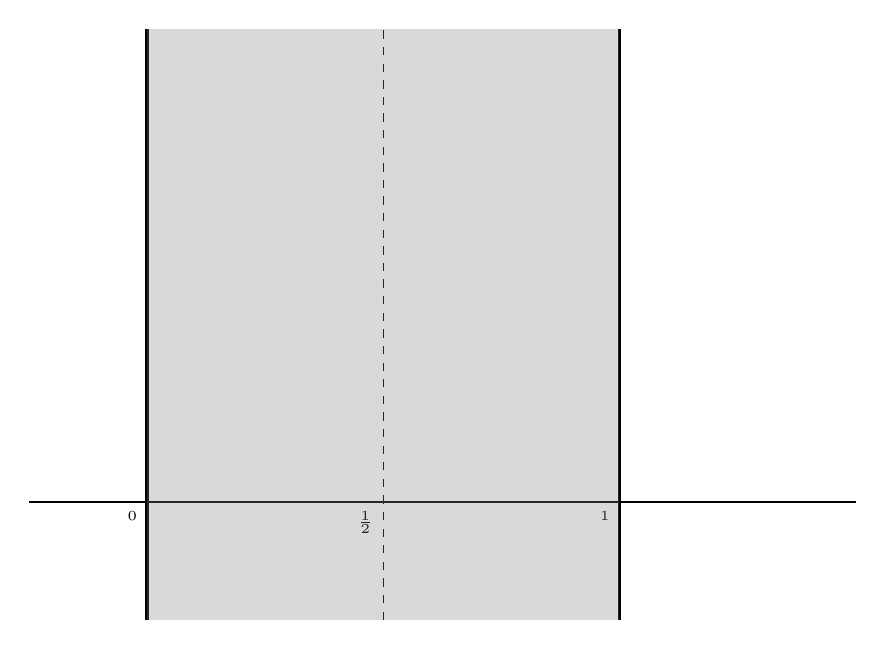
\begin{tikzpicture}[scale=3]
        \def\xmin{-0.5} \def\xmax{3}
        \def\ymin{-0.5} \def\ymax{2}
        \draw[thick] (\xmin,0) -- (\xmax,0);
        \draw[very thick] (0,\ymin) -- (0,\ymax);
        \draw[very thick] (2,\ymin) -- (2,\ymax);
        \draw[dashed] (1,\ymin) -- (1,\ymax);

        \node at (0,0) [below left] {\tiny{$0$}};
        \node at (1,0) [below left] {\tiny{$\frac{1}{2}$}};
        \node at (2,0) [below left] {\tiny{$1$}};

        \begin{scope}
          \path[clip] (0,\ymin) -- (0,\ymax) -- (2,\ymax) -- (2,\ymin) -- cycle;
          \fill[gray,opacity=0.3] (0,\ymin) rectangle (2,\ymax);
        \end{scope}
      \end{tikzpicture}
      \caption{The critical strip and critical line.}
      \label{fig:critical_strip}
    \end{figure}
  \section{The Approximate Functional Equation}
    If $L(s,f)$ is an $L$-function, then there is a formula which acts as a compromise between the functional equation for $L(s,f)$ and expressing $L(s,f)$ as a Dirichlet series. This formula is known as the approximate functional equation and it is important because it is valid inside of the critical strip and therefore can be used to obtain data about $L(s,f)$. First, we need to state an important asymptotic about the ratio of gamma factors that we will use later on. First suppose $\s$ is bounded and $|t| > 1$. This guarantees that $s$ is bounded away from zero so by \cref{equ:weaker_Stirling_formula}, we have
    \[
      \G(s) \sim \sqrt{2\pi}t^{\s-\frac{1}{2}}e^{-\frac{\pi}{2}|t|}.
    \]
    This gives the weaker estimates
    \[
      \G(s) \ll t^{\s-\frac{1}{2}}e^{-\frac{\pi}{2}|t|} \quad \text{and} \quad \frac{1}{\G(s)} \ll t^{\frac{1}{2}-\s}e^{\frac{\pi}{2}|t|} .
    \]
    It is not hard to obtain estimates that holds in vertical strips. Suppose $s$ is in the vertical strip $a < \s < b$ and is distance $\e$ away from the poles of $\G(s)$. For $|t| > 1$, the estimates above are satisfied. As these estimates are zero when $t = 0$ and $\G(s)$ is bounded on the compact region $a \le \s \le b$ with $|t| \le 1$ provided $s$ is distance $\e$ away from the poles, the estimates
    \begin{equation}\label{equ:modified_gamma_estimates}
      \G(s) \ll_{\e} (|t|+1)^{\s-\frac{1}{2}}e^{-\frac{\pi}{2}|t|} \quad \text{and} \quad \frac{1}{\G(s)} \ll_{\e} (|t|+1)^{\frac{1}{2}-\s}e^{\frac{\pi}{2}|t|},
    \end{equation}
    are valid in the vertical strip $a < \s < b$ and distance $\e$ away from the poles of $\G(s)$ in the first estimate. We immediately have the useful estimate
    \[
      \frac{\G(1-s)}{\G(s)} \ll_{\e} (|t|+1)^{1-2\s},
    \]
    valid in the is in the vertical strip $a < \s < b$ and distance $\e$ away from the poles of $\G(1-s)$. It easily follows from the definition of $\g(s,f)$ that
    \begin{equation}\label{equ:gamma_factor_analytic_conductor_estimate}
      \frac{\g(1-s,f)}{\g(s,f)} \ll_{\e} q_{\infty}(s,f)^{\frac{1-2\s}{2}} \quad \text{and} \quad q(f)^{\frac{s}{2}}\frac{\g(1-s,f)}{\g(s,f)} \ll_{\e} q(s,f)^{\frac{1-2\s}{2}},
    \end{equation}
    are valid in the is in the vertical strip $a < \s < b$ and is distance $\e$ away from the poles of $\g(1-s,f)$. We can use this last estimate to show that $L(s,f)$ is has polynomial growth in the $t$-aspect in vertical strips:

    \begin{proposition}\label{prop:L_function_bounded_in_vertical_strips}
      For any $L$-function $L(s,f)$ and $a < b$, $L(s,f)$ is of polynomial growth in the $t$-aspect in the vertical half-strip $a \le \s \le b$ with $|t| \ge 1$.
    \end{proposition}
    \begin{proof}
      On the one hand, for $\s > \max(1,b)$ we have $L(s,f) \ll 1$ on the line $\s = 1$ with $t \ge 1$. On the other hand, the functional equation and \cref{equ:gamma_factor_analytic_conductor_estimate} together imply
      \[
        L(s,f) \ll q(s,f)^{\frac{1-2\s}{2}}L(1-s,f).
      \]
      Clearly $q(s,f)^{\frac{1-2\s}{2}}$ is of polynomial growth in the $t$-aspect provided $\s$ is bounded. Thus for bounded $\s < \min(0,a)$, we see that $L(s,f)$ is also of polynomial growth in the $t$-aspect for $|t| \ge 1$. Moreover, this estimate also implies $L(s,f)$ is bounded on the line $t = 1$ provided $\s$ is bounded. As $L(s,f)$ is holomorphic for $|t| \ge 1$ and of order $1$, we can apply the Phragm\'en-Lindel\"of convexity principle in this region (see \cref{append:The_Phragmen_Lindelof_Convexity_principle}) so that $L(s,f)$ is of polynomial growth in the $t$-aspect in the vertical half-strip $a \le \s \le b$ with $|t| \ge 1$.
    \end{proof}

    \cref{prop:L_function_bounded_in_vertical_strips} is a very important property that $L$-functions possess. It is usually used to estimate Perron type formulas. We can also use it to deduce the \textbf{approximate function equation}\index{approximate function equation}:

    \begin{theorem}[Approximate functional equation]
      Let $L(s,f)$ be an $L$-function, $\Phi(u)$ be an even holomorphic function bounded in the vertical strip $|\Re(u)| < a+1$ for any $a > 1$ such that $\Phi(0) = 1$, and let $X > 0$. Then for $s$ in the critical strip, we have
      \[
        L(s,f) = \sum_{n \ge 1}\frac{a_{f}(n)}{n^{s}}V_{s}\left(\frac{n}{\sqrt{q(f)}X}\right)+\e(s,f)\sum_{n \ge 1}\frac{\conj{a_{f}(n)}}{n^{1-s}}V_{1-s}\left(\frac{nX}{\sqrt{q(f)}}\right)+\frac{R}{q(f)^{\frac{s}{2}}\g(s,f)},
      \]
      where $V_{s}(y):\R_{> 0} \to \C$ is the smooth function defined by
      \[
        V_{s}(y) = \frac{1}{2\pi i}\int_{(a)}\frac{\g(s+u,f)}{\g(s,f)}\Phi(u)y^{-u}\frac{du}{u},
      \]
      and
      \[
        \e(s,f) = \e(f)q(f)^{\frac{1}{2}-s}\frac{\g(1-s,f)}{\g(s,f)}.
      \]
      Moreover, the remainder $R$ is zero if $\L(s,f)$ is entire, and otherwise
      \[
        R = \left(\Res_{u = 1-s}+\Res_{u = -s}\right)\frac{\L(s+u,f)\Phi(u)X^{u}}{u}.
      \]
    \end{theorem}
    \begin{proof}
      Let
      \[
        I(X,s,f) = \frac{1}{2\pi i}\int_{(a)}\L(s+u,f)\Phi(u)X^{u}\,\frac{du}{u}.
      \]
      $L(s,f)$ has polynomial growth in the $t$-aspect by \cref{prop:L_function_bounded_in_vertical_strips}. From \cref{equ:modified_gamma_estimates} we see that $\g(s+u,f)$ has exponential decay. Since $\Phi(u)$ is bounded, it follows that the integrand has exponential decay in a vertical strip containing $|\Re(u)| \le a$. Therefore the integral is absolutely bounded by \cref{met:decay_compacta_integral}. Moreover, we may shift the line of integration to $(-a)$. In doing so, we pass by a simple pole at $u = 0$ and possible poles at $u = 1-s$ and $u = -s$, giving
      \[
        I(X,s,f) = \frac{1}{2\pi i}\int_{(-a)}\L(s+u,f)\Phi(u)X^{u}\,\frac{du}{u}+\L(s,f)+R.
      \]
      Applying the functional equation to $\L(s+u,f)$ and performing the change of variables $u \to -u$, we obtain
      \[
        I(X,s,f) = -\e(f)I(X^{-1},1-s,\conj{f})+\L(s,f)-R,
      \]
      since $\Phi(u)$ is even. This equation is equivalent to
      \[
        \L(s,f) = I(X,s,f)+\e(f)I(X^{-1},1-s,\conj{f})+R.
      \]
      Since $\Re(s+u) > 1$, we can expand the $L$-function $L(s,f)$ inside of $I(X,s,f)$ as a Dirichlet series:
      \begin{align*}
        I(X,s,f) &= \frac{1}{2\pi i}\int_{(a)}\L(s+u,f)\Phi(u)X^{u}\,\frac{du}{u} \\
        &= \frac{1}{2\pi i}\int_{(a)}q(f)^{\frac{s+u}{2}}\g(s+u,f)L(s+u,f)\Phi(u)X^{u}\,\frac{du}{u} \\
        &= \frac{1}{2\pi i}\int_{(a)}\sum_{n \ge 1}\frac{a_{f}(n)}{n^{s+u}}q(f)^{\frac{s+u}{2}}\g(s+u,f)\Phi(u)X^{u}\,\frac{du}{u} \\
        &= \sum_{n \ge 1}\frac{1}{2\pi i}\int_{(a)}\frac{a_{f}(n)}{n^{s+u}}q(f)^{\frac{s+u}{2}}\g(s+u,f)\Phi(u)X^{u}\,\frac{du}{u} && \text{DCT} \\
        &= q(f)^{\frac{s}{2}}\g(s,f)\sum_{n \ge 1}\frac{a_{f}(n)}{n^{s}}\frac{1}{2\pi i}\int_{(a)}\frac{\g(s+u,f)}{\g(s,f)}\Phi(u)\left(\frac{\sqrt{q(f)}X}{n}\right)^{u}\,\frac{du}{u} \\
        &= q(f)^{\frac{s}{2}}\g(s,f)\sum_{n \ge 1}\frac{a_{f}(n)}{n^{s}}V_{s}\left(\frac{n}{\sqrt{q(f)}X}\right).
      \end{align*}
      Performing the same computation for $I(X^{-1},1-s,\conj{f})$ and substituting in the results, we arrive at
      \[
        \L(s,f) = q(f)^{\frac{s}{2}}\g(s,f)\sum_{n \ge 1}\frac{a_{f}(n)}{n^{s}}V_{s}\left(\frac{n}{\sqrt{q(f)}X}\right)+\e(f)q(f)^{\frac{1-s}{2}}\g(1-s,f)\sum_{n \ge 1}\frac{a_{f}(n)}{n^{1-s}}V_{1-s}\left(\frac{nX}{\sqrt{q(f)}}\right)+R.
      \]
      Diving by $q(f)^{\frac{s}{2}}\g(s,f)$ completes the proof.
    \end{proof}

    The approximate functional equation was first developed by Hardy and Littlewood in the series \cite{hardyzeros1921,hardyapproximate1923,hardyapproximate1929}. The function $V_{s}(y)$ has the effect of smoothing out the two sums on the right-hand side of the approximate functional equation. To see this, we need  the following proposition:

    \begin{proposition}\label{prop:V_function_decay}
      Let $L(s,f)$ be an $L$-function and $\Phi(u)$ be an even holomorphic function bounded in the vertical strip $|\Re(u)| < a+1$ for any $a > 1$ such that $\Phi(0) = 1$. Let $V_{s}(y):\R_{> 0} \to \C$ be the smooth function defined by
      \[
        V_{s}(y) = \frac{1}{2\pi i}\int_{(a)}\frac{\g(s+u,f)}{\g(s,f)}\Phi(u)y^{-u}\frac{du}{u}.
      \]
      For $s$ in the critical strip, $V_{s}(y)$ satisfies the estimate
      \[
        V_{s}(y) \ll \left(1+\frac{y}{\sqrt{q_{\infty}(s,f)}}\right)^{-a}.
      \]
    \end{proposition}
    \begin{proof}
      Let $u = \tau+ir$ and suppose $0 \le \s \le \frac{1}{2}$ so that $\s-\frac{1}{2} \le 0$. Then from \cref{equ:modified_gamma_estimates} and the reverse triangle inequality (in the form $|t+r| \ge ||r|-|t||$), we deduce that
      \[
        \frac{\G(s+u)}{\G(s)} \ll \frac{(|t+r|+1)^{\s+\tau-\frac{1}{2}}}{(|t|+1)^{\s-\frac{1}{2}}}e^{\frac{\pi}{2}(|t|-|t+r|)} \ll (|t+r|+1)^{\tau}e^{-\frac{\pi}{2}|r|}.
      \]
      From the definition of the analytic conductor, the above estimate implies
      \[
        \frac{\g(s+u,f)}{\g(s,f)} \ll q_{\infty}(s,f)^{\frac{\tau}{2}}e^{-\frac{\pi}{2}d|r|},
      \]
      for $s$ in the critical strip. The fact tht $\Phi(u)$ is bounded, $u$ is bounded away from zero, and the estimate for the ratio of gamma factors gives the first estimate in the following chain:
      \begin{align*}
        V_{s}(y) &= \frac{1}{2\pi i}\int_{(a)}\frac{\g(s+u,f)}{\g(s,f)}\Phi(u)y^{-u}\frac{du}{u} \\
        &\ll \int_{-\infty}^{\infty}q_{\infty}(s,f)^{\frac{a}{2}}e^{-\frac{\pi}{2}d|r|}y^{-a}\,dr \\
        &\ll \int_{-\infty}^{\infty}q_{\infty}(s,f)^{\frac{a}{2}}e^{-\frac{\pi}{2}d|r|}(1+y)^{-a}\,dr \\
        &\ll \int_{-\infty}^{\infty}e^{-\frac{\pi}{2}d|r|}\left(1+\frac{y}{\sqrt{q_{\infty}(s,f)}}\right)^{-a}\,dr \\
        &\ll \left(1+\frac{y}{\sqrt{q_{\infty}(s,f)}}\right)^{-a}\int_{-\infty}^{\infty}e^{-\frac{\pi}{2}d|r|}\,dr \\
        &\ll \left(1+\frac{y}{\sqrt{q_{\infty}(s,f)}}\right)^{-a},
      \end{align*}
      where in the third and fourth lines we have used that $cy \ll (1+cy)$ for all $y \in \R_{> 0}$ and any $c$ and the last line holds by \cref{met:decay_compacta_integral} since $e^{-\frac{\pi}{2}d|r|}$ has exponential decay. This completes the proof.
    \end{proof}

    From \cref{prop:V_function_decay} we see that $V_{s}(f)$ is bounded for $y \ll q_{\infty}(s,f)^{\frac{1}{2}+\e}$ and then starts to exhibit polynomial decay.
  \section{The Riemann Hypothesis \& Nontrivial Zeros}
    The zeros of $L$-functions $L(s,f)$ are closely tied to important arithmetic data of $f$. Let $L(s,f)$ be a degree $d$ $L$-function so that
    \[
      L(s,f) = \prod_{p}(1-\a_{1}(p)p^{-s})^{-1}(1-\a_{2}(p)p^{-s})^{-1} \cdots (1-\a_{d}(p)p^{-s})^{-1},
    \]
    for $\s > 1$. This product vanishes if and only if one of its factors are zero. As $\s > 1$, this is impossible so that $L(s,f)$ has no zeros in this region. The functional equation will allow us to understand more about the zeros of $L(s,f)$. Rewrite the functional equation for $L(s,f)$ as
    \begin{equation}\label{equ:fun_eq_for_zeros}
      L(s,f) = \e(f)q(f)^{\frac{1}{2}-s}\frac{\g(1-s,f)}{\g(s,f)}L(1-s,\conj{f}).
    \end{equation}
    If $\s < 0$ then $L(1-s,\conj{f})$ is nonzero by our previous comments. Moreover, $\g(1-s,f)$ is holomorphic in this region because $\Re(\k_{i}) \ge -1$ for all $i$. We conclude that poles of $\g(s,f)$ are zeros of $L(s,f)$ for $\s < 0$. Such zeros are called \textbf{trivial zeros}\index{trivial zeros}. From the definition of $\g(s,f)$, they are all simple and are of the form $s = \k_{i}-2n$ for some local root at infinity $\k_{i}$ and some integer $n \ge 0$. Any other zero of $L(s,f)$ is called a \textbf{nontrivial zeros}\index{nontrivial zeros} and it lies inside of the critical strip.

    \begin{remark}\label{rem:poles_of_completed_L_function}
      Recall that for any $L$-function $L(s,f)$, the completed $L$-function $\L(s,f)$ is required to be meromorphic on $\C$ with at most poles at $s = 0$ and $s = 1$. We have shown that the trivial zeros of $L(s,f)$ are poles of $\g(s,f)$ for $\s < 0$ and they are all simple. As $L(s,f)$ is meromorphic on $\C$ with at most a pole at $s = 1$, and $\g(s,f)$ has at most poles at $s = 0$ and $s = 1$ for $\s \ge 0$, $\L(s,f)$ is meromorphic on $\C$ with at most poles at $s = 0$ and $s = 1$.
    \end{remark}
    
    Now let $\rho$ be a nontrivial zero of $L(s,f)$. Note that $\conj{L(s,f)} = L(\conj{s},\conj{f})$ by the identity theorem and that this equality holds for $\s > 1$ where $L(s,f)$ is defined by a Dirichlet series. It follows that $\conj{\rho}$ is a nontrivial zero of $L(s,\conj{f})$. In the interior of critical strip, the gamma factor is nonzero and holomorphic (again we have used $\Re(\k_{i}) \ge 1$ for all $i$). From the functional equation, it follows that $1-\conj{\rho}$ is also a nontrivial zero of $L(s,f)$. In short, the nontrivial zeros occur in pairs:
    \[
      \rho \quad \text{and} \quad 1-\conj{\rho}.
    \]
    We can sometimes say more. If $L(s,f)$ takes real values for $s > 1$, the Schwarz reflection principle implies $L(\conj{s},f) = \conj{L(s,f)}$ and that $L(s,f)$ takes real values on the entire real axis save for the possible poles at $s = 0$ and $ s = 1$. We find that $\conj{\rho}$ and $1-\conj{\rho}$ are nontrivial zeros too and therefore the nontrivial zeros of $L(s,f)$ come in sets of four:
    \[
      \rho, \quad \conj{\rho}, \quad 1-\rho, \quad \text{and} \quad 1-\conj{\rho}.
    \]
    The \textbf{(Selberg class) Riemann hypothesis}\index{(Selberg class) Riemann hypothesis} says that this symmetry should be as simple as possible:

    \begin{conjecture}[Riemann hypothesis, Selberg class version]
      All of the nontrivial zeros of any $L$-function $L(s,f)$ belonging to the Selberg class lie on the line $\s = \frac{1}{2}$.
    \end{conjecture}
  \section{The Lindel\"of Hypothesis \& Convexity Arguments}
    Instead of asking about the zeros of an $L$-function $L(s,f)$ on the critical line, we can ask about the growth of $L(s,f)$ on the critical line. A \textbf{convexity argument}\index{convexity argument} is one where estimates about the growth of an $L$-function on the critical line are deduced. Usually this is achieved by methods of complex analysis and Sirling's formula. The standard argument for any $L$-function is known \textbf{Lindel\"of convexity argument}\index{Lindel\"of convexity argument}. It is essentially a refinement of the proof of \cref{prop:L_function_bounded_in_vertical_strips}. Suppose $L(s,f)$ has a degree $d$ Euler product. Also suppose $L(s,f)$ as a pole of order $r \ge 0$ at $s = 1$ and let
    \[
      p_{r}(s) = \left(\frac{s-1}{s+1}\right)^{r}.
    \]
    Note that $p_{r}(s) \sim 1$. The first step is to guarantee the Phragm\'en-Lindel\"of convexity principle for $p_{r}(s)L(s,f)$ in a region containing the critical strip. As $L(s,f)$ is of order $1$, this is assured (see \cref{append:The_Phragmen_Lindelof_Convexity_principle}). Therefore, we are reduced to estimating the growth of $p_{r}(s)L(s,f)$ for $\s$ to the left of $0$ and to the right of $1$. That is, just outside the edges of the critical strip. The right edge is easily estimated by setting $\s = 1+\e$ so that
    \[
      p_{r}(1+\e+it)L(1+\e+it,f) \ll_{\e} 1.
    \]
    The left edge is only slightly more difficult. The functional equation and \cref{equ:gamma_factor_analytic_conductor_estimate} together imply
    \[
      p_{r}(s)L(s,f) \ll p_{r}(s)q(s,f)^{\frac{1-2\s}{2}}L(1-s,f),
    \]
    for $s$ in any vertical strip with distance $\e$ away from the poles of $\g(1-s,f)$. Setting $\s = -\e$, we obtain
    \[
      p_{r}(-\e+it)L(-\e+it,f) \ll_{\e} q(s,f)^{\frac{1}{2}+\e}.
    \]
    As $p_{r}(s)L(s,f)$ is holomorphic in a region containing the vertical strip $-\e \le \s \le 1+\e$, the Phragm\'en-Lindel\"of convexity principle gives
    \[
      L(s,f) \ll_{\e} q(s,f)^{\frac{1-\s}{2}+\e},
    \]
    in the vertical strip $-\e \le \s \le 1+\e$. At the critical line, we have the \textbf{convexity bound}\index{convexity bound}:
    \begin{equation}\label{equ:convexity_bound_L_function}
      L\left(\frac{1}{2}+it,f\right) \ll_{\e} q\left(\frac{1}{2}+it,f\right)^{\frac{1}{4}+\e}.
    \end{equation}
    The \textbf{(Selberg class) Lindel\"of hypothesis}\index{(Selberg class) Lindel\"of hypothesis} says that the exponent can be reduced to $\e$:

    \begin{conjecture}[Lindel\"of hypothesis, Selberg class version]
      For any $L$-function $L(s,f)$ belonging to the Selberg class, we have
      \[
        L\left(\frac{1}{2}+it,f\right) \ll_{\e} q\left(\frac{1}{2}+it,f\right)^{\e}.
      \]
    \end{conjecture}

    Any improvement upon the exponent in the convexity bound in any aspect of the analytic conductor is called a \textbf{subconvexity estimate}\index{subconvexity estimate} (or a \textbf{convexity breaking bound}\index{convexity breaking bound}). Any argument used to do so is called a \textbf{subconvexity argument}\index{subconvexity argument}.
  \section{Estimating the Central Value}
    The Lindel\"of hypothesis is concerned with the growth of the $L$-function $L(s,f)$ along the critical line. Sometimes we are only concerned with the size of $L(s,f)$ when $s = \frac{1}{2}$. The point $s = \frac{1}{2}$ is called the \textbf{central value}\index{central value} of $L(s,f)$ since it is exactly the midpoint on the critical line. Many important properties about $L(s,f)$ can be connected to its size at the central value. Any argument used to estimate an $L$-function at the central value is called a \textbf{central value estimate}\index{central value estimate}. We will state a result which gives a very useful upper bound for the size of an $L$-function at the central value in the $q(f)$-aspect. To state it, let $\psi:\R_{\ge 0} \to \R_{\ge 0}$ be a bump function with compact support in $\left[\frac{1}{2},2\right]$. Explicitly,
    \[
      \psi(y) = \begin{cases} e^{-\frac{1}{9-(4y-5)^{2}}} & \text{if $|4y-5| < 3$}, \\ 0 & \text{if $|4y-5| \ge 3$}. \end{cases}
    \]
    The theorem is the following:

    \begin{theorem}
      Let $L(s,f)$ be an $L$-function and let $\psi:\R_{\ge 0} \to \R_{\ge 0}$ be a bump function with compact support in $\left[\frac{1}{2},2\right]$. Then we have
      \[
        L\left(\frac{1}{2},f\right) \ll_{\e} \max_{X \ll q(f)^{\frac{1}{2}+\e}}\frac{A_{\psi}(X)}{q(f)^{\frac{1}{4}}}+\frac{S}{q(f)^{\frac{1}{4}}},
      \]
      where $S$ is zero if $\L(s,f)$ is entire, and otherwise
      \[
        S = \left(\Res_{u = \frac{1}{2}}+\Res_{u = -\frac{1}{2}}\right)\L\left(\frac{1}{2}+u,f\right).
      \]
    \end{theorem}
    \begin{proof}
      Taking $s = \frac{1}{2}$ and $X = 1$ in the approximate functional equation gives
      \[
        L\left(\frac{1}{2},f\right) = \sum_{n \ge 1}\frac{a_{f}(n)}{\sqrt{n}}V_{\frac{1}{2}}\left(\frac{n}{\sqrt{q(f)}}\right)+\e(f)\sum_{n \ge 1}\frac{\conj{a_{f}(n)}}{\sqrt{n}}V_{\frac{1}{2}}\left(\frac{n}{\sqrt{q(f)}}\right)+\frac{R}{q(f)^{\frac{1}{4}}\g\left(\frac{1}{2},f\right)}.
      \]
      This implies the bound
      \[
        L\left(\frac{1}{2},f\right) \ll \sum_{n \ge 1}\frac{a_{f}(n)}{\sqrt{n}}V_{\frac{1}{2}}\left(\frac{n}{\sqrt{q(f)}}\right)+\frac{S}{q(f)^{\frac{1}{4}}}.
      \]
      Now consider the set of functions $\left\{\psi\left(\frac{y}{2^{k}}\right)\right\}_{k \in \Z}$. Since $\psi\left(\frac{y}{2^{k}}\right)$ has support in $[2^{k-1},2^{k+1}]$, the sum $\s(y) = \sum_{k \in \Z}\psi\left(\frac{y}{2^{k}}\right)$, defined for $y \ge 0$, is finite since at most finitely many terms are nonzero for every $y$. It is also bounded away from zero since for any $x > 0$ there is some $k \in \Z$ for which $2^{k} \le y \le 3 \cdot 2^{k-1}$ so that $\frac{y}{2^{k}}$ is at least distance $\frac{1}{2}$ from the endpoints of $\left[\frac{1}{2},2\right]$. Defining $\psi_{k}(y) = \psi\left(\frac{y}{2^{k}}\right)\s(y)^{-1}$, it follows that $\left\{\psi_{k}(y)\right\}_{k \in \Z}$ satisfies
      \[
        \sum_{k \in \Z}\psi_{k}(y) = 1,
      \]
      for any $y \in \R_{> 0}$. Then we can write
      \begin{align*}
        V_{s}(y) &= \frac{1}{2\pi i}\int_{(a)}\frac{\g(s+u,f)}{\g(s,f)}\Phi(u)y^{-u}\frac{du}{u} \\
        &= \frac{1}{2\pi i}\int_{(a)}\sum_{k \in \Z}\frac{\g(s+u,f)}{\g(s,f)}\Phi(u)y^{-u}\psi_{k}(y)\frac{du}{u} \\
        &= \sum_{k \in \Z}\frac{1}{2\pi i}\int_{(a)}\frac{\g(s+u,f)}{\g(s,f)}\Phi(u)y^{-u}\psi_{k}(y)\frac{du}{u} && \text{DCT} \\
        &= \sum_{k \in \Z}V_{s,k}(y),
      \end{align*}
      where we have set
      \[
        V_{s,k}(y) = \frac{1}{2\pi i}\int_{(a)}\frac{\g(s+u,f)}{\g(s,f)}\Phi(u)y^{-u}\psi_{k}(y)\frac{du}{u}.
      \]
      Note that $V_{s,k}(y)$ is compactly supported on $[2^{k-1},2^{k}]$ because $\psi_{k}(y)$ is compactly supported there. Moreover, \cref{prop:V_function_decay} implies that $V_{s,k}(y)$ also exhibits polynomial decay for $y \gg q_{\infty}(s,f)^{\frac{1}{2}+\e}$. It follows that
      \[
        \sum_{n \ge 1}\frac{a_{f}(n)}{\sqrt{n}}V_{\frac{1}{2}}\left(\frac{n}{\sqrt{q(f)}}\right) = \sum_{k \in \Z}\sum_{2^{k-1} \le n \le 2^{k+1}}\frac{a_{f}(n)}{\sqrt{n}}V_{\frac{1}{2},k}\left(\frac{n}{\sqrt{q(f)}}\right).
      \]
      Using the polynomial decay of $V_{\frac{1}{2},k}(y)$ to bound those terms for which $n \gg q\left(\frac{1}{2},f\right)^{\frac{1}{2}+\e} \gg q(f)^{\frac{1}{2}+\e}$ gives the estimate
      \[
        \sum_{n \ge 1}\frac{a_{f}(n)}{\sqrt{n}}V_{\frac{1}{2}}\left(\frac{n}{\sqrt{q(f)}}\right) \ll \sum_{k \ll q(f)^{\e}}\sum_{\substack{2^{k-1} \le n \le 2^{k+1} \\ n \ll q(f)^{\frac{1}{2}+\e}}}\frac{a_{f}(n)}{\sqrt{n}}V_{\frac{1}{2},k}\left(\frac{n}{\sqrt{q(f)}}\right),
      \]
      where in the first sum we have used that $\log(y) \ll_{\e} y^{\e}$. Now since $\s(y)$ is bounded away from zero and $V_{\frac{1}{2},k}(y)$ and $\psi(y)$ are compactly supported on the same interval (so their nonzero values differ by a bounded amount), we have the weaker estimate
      \[
        \sum_{n \ge 1}\frac{a_{f}(n)}{\sqrt{n}}V_{\frac{1}{2}}\left(\frac{n}{\sqrt{q(f)}}\right) \ll_{\e} q(f)^{\e}\max_{X \ll q(f)^{\frac{1}{2}+\e}}\sum_{\frac{X}{2} \le n \le 2X}\frac{a_{f}(n)}{\sqrt{n}}\psi\left(\frac{n}{\sqrt{q(f)}}\right).
      \]
      We will estimate this latter sum. Abel's summation formula (see \cref{{append:Summation_Formulas}}) gives
      \[
        \sum_{\frac{X}{2} \le n \le 2X}\frac{a_{f}(n)}{\sqrt{n}}\psi\left(\frac{n}{X}\right) = \frac{A_{\psi}(2X)}{\sqrt{2X}}-\frac{A_{\psi}\left(\frac{X}{2}\right)}{\sqrt{\frac{X}{2}}}+\frac{1}{2}\int_{\frac{X}{2}}^{2X}A_{\psi}(u)u^{-\frac{3}{2}}\,du.
      \]
      But as
      \[
        \frac{1}{2}\int_{\frac{X}{2}}^{2X}A_{\psi}(u)u^{-\frac{3}{2}}\,du \ll X\max_{\frac{X}{2} \le u \le 2X}A_{\psi}(u)u^{-\frac{3}{2}} \ll \max_{\frac{X}{2} \le u \le 2X}\frac{A_{\psi}(u)}{\sqrt{u}},
      \]
      we obtain the bound
      \[
        \max_{X \ll q(f)^{\frac{1}{2}+\e}}\sum_{\frac{X}{2} \le n \le 2X}\frac{a_{f}(n)}{\sqrt{n}}\psi\left(\frac{n}{X}\right) \ll \max_{X \ll q(f)^{\frac{1}{2}+\e}}\frac{A_{\psi}(X)}{\sqrt{X}}.
      \]
      Putting everything together gives
      \[
        \sum_{n \ge 1}\frac{a_{f}(n)}{\sqrt{n}}V_{\frac{1}{2}}\left(\frac{n}{\sqrt{q(f)}}\right) \ll_{\e} q(f)^{\frac{\e}{2}}\max_{X \ll q(f)^{\frac{1}{2}+\e}}\frac{A_{\psi}(X)}{\sqrt{X}} \ll_{\e} \max_{X \ll q(f)^{\frac{1}{2}+\e}}\frac{A_{\psi}(X)}{q(f)^{\frac{1}{4}}},
      \]
      where in the last estimate we may replace $X$ with $q(f)^{\frac{1}{2}+\e}$ because $X \ge 1$ so that $X$ is bounded away from zero.
    \end{proof}
  \chapter{Types of \texorpdfstring{$L$}{L}-functions}
  We discuss a variety of $L$-functions: the Riemann zeta function, $L$-functions attached to Dirichlet characters, and Hecke $L$-functions. In the case of Hecke $L$-functions, we also describe a method of Rankin and Selberg for constructing new $L$-functions from old ones.
  \section{The Riemann Zeta Function}
    \subsection*{The Definition \& Euler Product of \texorpdfstring{$\z(s)$}{\z(s)}}
      The \textbf{Riemann zeta function}\index{Riemann zeta function} or simply the \textbf{zeta function}\index{zeta function} $\z(s)$ is defined as an $L$-series:
      \[
        \z(s) = \sum_{n \ge 1}\frac{1}{n^{s}}.
      \]
      This is the prototypical example of a Dirichlet series as all the coefficients are $1$. We will see that $\z(s)$ is a Selberg class $L$-function. As the coefficients are trivially polynomially bounded, $\z(s)$ is locally absolutely uniformly convergent for $\s > 1$. Also note that $\z(s)$ is necessarily nonzero in this region. Determining the Euler product is also an easy matter. As the coefficients are obviously completely multiplicative, we have the degree $1$ Euler product:
      \[
        \z(s) = \prod_{p}(1-p^{-s})^{-1},
      \]
      in this region as well. The local factor at $p$ is $\z_{p}(s) = (1-p^{-s})^{-1}$ with local root $1$.
    \subsection*{The Integral Representation of \texorpdfstring{$\z(s)$}{\z(s)}: Part I}
      Riemann's ingenious insight was to analytically continue $\z(s)$. By this, he sought to find a representation of $\z(s)$ defined on a larger region than $\s > 1$. This is the approach we will take, and the argument follows the same line of reasoning as that of Riemann. We consider the gamma function $\G\left(\frac{s}{2}\right)$:
      \[
        \G\left(\frac{s}{2}\right) = \int_{0}^{\infty}e^{-x}x^{\frac{s}{2}}\,\frac{dx}{x}.
      \]

      \begin{remark}
        We have chosen to express the gamma function in terms of the measure $\frac{dx}{x}$ instead of $dx$. This is a tactical change for two reasons. The first is that $\frac{dx}{x}$ is invariant under the change of variables $x \to Cx$ for any constant $C$. The second is that under the change of variables $x \to \frac{1}{x}$ we have $\frac{dx}{x} \to -\frac{dx}{x}$ but the bounds of integration are also flipped. So we may leave the measure invariant provided we don't flip the bounds of integration. These types of change of variables are essential in the study of $L$-functions which motivates the use of this measure.
      \end{remark}

      Performing the change of variables $x \to \pi n^{2}x$ for fixed $n \ge 1$ yields
      \begin{equation}\label{equ:gamma_integral_substitution}
        \G\left(\frac{s}{2}\right) = \pi^{\frac{s}{2}} n^{s}\int_{0}^{\infty}e^{-\pi n^{2}x}x^{\frac{s}{2}}\,\frac{dx}{x}.
      \end{equation}
      Let $\s > 1$. Dividing by $\pi^{\frac{s}{2}}n^{s}$ and summing over $n \ge 1$, we see that
      \begin{align*}
        \pi^{-\frac{s}{2}}\G\left(\frac{s}{2}\right)\z(s) &= \sum_{n \ge 1}\int_{0}^{\infty}e^{-\pi n^{2}x}x^{\frac{s}{2}}\,\frac{dx}{x} \\
        &= \int_{0}^{\infty}\sum_{n \ge 1}e^{-\pi n^{2}x}x^{\frac{s}{2}}\,\frac{dx}{x} && \text{DCT} \\
        &= \int_{0}^{\infty}\w(x)x^{\frac{s}{2}}\,\frac{dx}{x},
      \end{align*}
      where we set
      \[
        \w(x) = \sum_{n \ge 1}e^{-\pi n^{2}x}.
      \]
      Therefore we have an integral representation
      \begin{equation}\label{equ:integral_representation_zeta_1}
        \z(s) = \frac{\pi^{\frac{s}{2}}}{\G\left(\frac{s}{2}\right)}\int_{0}^{\infty}\w(x)x^{\frac{s}{2}}\,\frac{dx}{x}.
      \end{equation}
      This was essentially Riemann's insight: rewrite the Riemann zeta function in terms of a Mellin transform. Unfortunately, we cannot proceed until we understand $\w(x)$. So we will make a slight detour and come back to the integral representation after.
    \subsection*{Jacobi's Theta Function \texorpdfstring{$\vt(s)$}{\vt(s)}}
      \textbf{Jacobi's theta function}\index{Jacobi's theta function} $\vt(s)$ is defined for $\s > 0$ by
      \[
        \vt(s) = \sum_{n \in \Z}e^{-\pi n^{2}s} = 1+2\sum_{n \ge 1}e^{-\pi n^{2}s}.
      \]
      It is locally absolutely uniformly convergent in this region by the ratio test. Its relation to $\w(s)$ is given by the identity
      \begin{equation}\label{equ:omega_theta_relationship_for_zeta}
        \w(s) = \frac{\vt(s)-1}{2}.
      \end{equation}
      We see from the Taylor series of $\frac{1}{1-e^{\s}}$, that
      \[
        \w(s) = O\left(\sum_{n \ge 1}e^{-\pi n^{2}\s}\right) = O\left(\sum_{n \ge 1}e^{-\pi n\s}\right) = O\left(\frac{1}{1-e^{-\pi\s}}\right) = O(e^{-\pi\s}),
      \]
      and so $\w(s)$ exhibits rapid decay. The essential fact about Jacobi's theta function we will need is the \textbf{functional equation for Jacobi's theta function}\index{functional equation for Jacobi's theta function} that was known to Riemann:

      \begin{theorem}[Functional equation for Jacobi's theta function]
        For $\s > 0$,
        \[
          \vt(s) = \frac{1}{\sqrt{s}}\vt\left(\frac{1}{s}\right).
        \]
      \end{theorem}
      \begin{proof}
        By the identity theorem it suffices to verify this for $s = \s$ with $\s > 0$. Set $f(x) = e^{-\pi x^{2}s}$. Then $f(x)$ is of Schwarz class. We compute its Fourier transform:
        \[
          \hat{f}(t) = \int_{-\infty}^{\infty}f(x)e^{-2\pi itx}\,dx = \int_{-\infty}^{\infty}e^{-\pi x^{2}s}e^{-2\pi itx}\,dx = \int_{-\infty}^{\infty}e^{-\pi(x^{2}s+2itx)}\,dx.
        \]
        Making the change of variables $x \to \frac{x}{\sqrt{s}}$, the last integral above becomes
        \[
          \frac{1}{\sqrt{s}}\int_{-\infty}^{\infty}e^{-\pi\left(x^{2}+\frac{2itx}{\sqrt{s}}\right)}.
        \]
        Complete the square in the exponent by noticing
        \[
          -\pi\left(x^{2}+\frac{2itx}{\sqrt{s}}\right) = -\pi\left(\left(x+\frac{it}{\sqrt{s}}\right)^{2}+\frac{t^{2}}{s^{2}}\right).
        \]
        Taking exponentials, this implies that the previous integral is equal to
        \[
          \frac{e^{-\frac{\pi t^{2}}{s}}}{\sqrt{s}}\int_{-\infty}^{\infty}e^{-\pi\left(x+\frac{it}{\sqrt{s}}\right)^{2}}\,dx.
        \]
        The change of variables $x \to \frac{x}{\sqrt{s}}-\frac{it}{\sqrt{s}}$ is permitted without affecting the line of integration by viewing the integral as a complex integral, noting that the integrand is entire as a complex function, and shifting the line of integration. This gives
        \[
          \frac{e^{-\frac{\pi t^{2}}{s}}}{\sqrt{s}}\int_{-\infty}^{\infty}e^{-\pi\left(x+\frac{it}{\sqrt{s}}\right)^{2}}\,dx = \frac{e^{-\frac{\pi t^{2}}{s}}}{\sqrt{s}}\int_{-\infty}^{\infty}e^{-\pi x^{2}}\,dx = \frac{e^{-\frac{\pi t^{2}}{s}}}{\sqrt{s}},
        \]
        where the last equality follows because the last integral above is $1$ since it is the Gaussian integral (see \cref{append:Special_Integrals}). Thus
        \[
          \hat{f}(t) = \frac{e^{-\frac{\pi t^{2}}{s}}}{\sqrt{s}}.
        \]
        By the Poisson summation formula, we have
        \[
          \vt(s) = \sum_{t \in \Z}\frac{e^{-\frac{\pi t^{2}}{s}}}{\sqrt{s}} = \frac{1}{\sqrt{s}}\sum_{t \in \Z}e^{-\frac{\pi t^{2}}{s}} = \frac{1}{\sqrt{s}}\vt\left(\frac{1}{s}\right),
        \]
        and the identity theorem finishes the proof.
      \end{proof}

      We will use this functional equation to analytically continue $\z(s)$.
    \subsection*{The Integral Representation of \texorpdfstring{$\z(s)$}{\z(s)}: Part II}
      Returning to the Riemann zeta function, we split the integral in \cref{equ:integral_representation_zeta_1} into two pieces
      \begin{equation}\label{equ:symmetric_integral_zeta_split}
        \int_{0}^{\infty}\w(x)x^{\frac{s}{2}}\,\frac{dx}{x} = \int_{0}^{1}\w(x)x^{\frac{s}{2}}\,\frac{dx}{x}+\int_{1}^{\infty}\w(x)x^{\frac{s}{2}}\,\frac{dx}{x}.
      \end{equation}
      Since $\w(x)$ has rapid decay, the second piece is locally absolutely uniformly convergent for $\s > 1$ by \cref{prop:decay_unbounded_inteval_integral}. Hence it is analytic there. The idea now is to rewrite the first piece in the same form and symmetrize the result as much as possible. We being by performing a change of variables $x \to \frac{1}{x}$ to the first piece to obtain
      \[
        \int_{1}^{\infty}\w\left(\frac{1}{x}\right)x^{-\frac{s}{2}}\,\frac{dx}{x}
      \]
      Now the functional equation for Jacobi's theta function $\vt(x)$ and \cref{equ:omega_theta_relationship_for_zeta} together imply
      \begin{equation}\label{equ:piece_one_zeta_1}
        \w\left(\frac{1}{x}\right) = \frac{\vt\left(\frac{1}{x}\right)-1}{2} = \frac{\sqrt{x}\vt(x)-1}{2} = \frac{\sqrt{x}(2\w(x)+1)-1}{2} = \sqrt{x}\w(x)+\frac{\sqrt{x}}{2}-\frac{1}{2}.
      \end{equation}
      \cref{equ:piece_one_zeta_1} gives the first equality in the following chain:
      \begin{align*}
        \int_{1}^{\infty}\w\left(\frac{1}{x}\right)x^{-\frac{s}{2}}\,\frac{dx}{x} &= \int_{1}^{\infty}\left(\sqrt{x}\w(x)+\frac{\sqrt{x}}{2}-\frac{1}{2}\right)x^{-\frac{s}{2}}\,\frac{dx}{x} \\
        &= \int_{1}^{\infty}\w(x)x^{\frac{1-s}{2}}\,\frac{dx}{x}+\int_{1}^{\infty}\frac{x^{\frac{1-s}{2}}}{2}\,\frac{dx}{x}-\int_{1}^{\infty}\frac{x^{-\frac{s}{2}}}{2}\,\frac{dx}{x} \\
        &= \int_{1}^{\infty}\w(x)x^{\frac{1-s}{2}}\,\frac{dx}{x}+\frac{1}{1-s}-\frac{1}{s} \\
        &= \int_{1}^{\infty}\w(x)x^{\frac{1-s}{2}}\,\frac{dx}{x}-\frac{1}{s(1-s)}.
      \end{align*}
      Substituting this result back into \cref{equ:symmetric_integral_zeta_split} with \cref{equ:integral_representation_zeta_1} yields the integral representation
      \[
        \z(s) = \frac{\pi^{\frac{s}{2}}}{\G\left(\frac{s}{2}\right)}\left[-\frac{1}{s(1-s)}+\int_{1}^{\infty}\w(x)x^{\frac{1-s}{2}}\,\frac{dx}{x}+\int_{1}^{\infty}\w(x)x^{\frac{s}{2}}\,\frac{dx}{x}\right].
      \]
      This integral representation will give analytic continuation. To see this, first observe that everything outside the brackets is entire. Moreover, the two integrals are locally absolutely uniformly convergent on $\C$ by \cref{prop:decay_unbounded_inteval_integral}. The fractional term is holomorphic except for simple poles at $s = 0$ and $s = 1$. The meromorphic continuation to $\C$ follows with possible simple poles at $s = 0$ and $s = 1$. There is no pole at $s = 0$. Indeed, $\g(s,\z)$ has a simple pole coming from the gamma factor there and so its reciprocal has a simple zero. This cancels the corresponding simple pole of $\frac{1}{s(1-s)}$ so that $\z(s)$ has a removable singularity and thus is holomorphic at $s = 0$. At $s = 1$, $\g(s,\z)$ is nonzero, and so $\z(s)$ has a simple pole. Therefore $\z(s)$ has meromorphic continuation to all of $\C$ with a simple pole at $s = 1$. 
    \subsection*{The Functional Equation, Critical Strip \& Residue of \texorpdfstring{$\z(s)$}{\z(s)}}
      An immediate consequence of applying the symmetry $s \to 1-s$ to the integral representation is the following functional equation:
      \[
        \frac{\G\left(\frac{s}{2}\right)}{\pi^{\frac{s}{2}}}\z(s) = \frac{\G\left(\frac{1-s}{2}\right)}{\pi^{\frac{1-s}{2}}}\z(1-s).
      \]
      We identify the gamma factor as
      \[
        \g(s,\z) = \pi^{-\frac{s}{2}}\G\left(\frac{s}{2}\right),
      \]
      with $\k = 0$ the only local root at infinity. Clearly it satisfies the required bounds. The conductor is $q(\z) = 1$ so no primes ramify. The completed zeta function is
      \[
        \L(s,\z) = \pi^{-\frac{s}{2}}\G\left(\frac{s}{2}\right)\z(s),
      \]
      with functional equation
      \[
        \L(s,\z) = \L(1-s,\z).
      \]
      This is the functional equation of $\z(s)$ and in this case is just a reformulation of the previous functional equation. From it we find that the root number is $\e(\z) = 1$ and that $\z(s)$ is self-dual. We can now show that the order of $\z(s)$ is $1$. As there is only a simple pole at $s = 1$, multiply by $(s-1)$ to clear the polar divisor. As the integrals in the integral representation are locally absolutely uniformly convergent, computing the order amounts to estimating the gamma factor. Since the reciprocal of the gamma function is of order $1$, we have
      \[
        \frac{1}{\g(s,\z)} \ll_{\e} e^{|s|^{1+\e}}.
      \]
      Thus the reciprocal of the gamma factor is also of order $1$. It follows that
      \[
        (s-1)\z(s) \ll_{\e} e^{|s|^{1+\e}}.
      \]
      This shows $(s-1)\z(s)$ is of order $1$, and thus $\z(s)$ is as well after removing the polar divisor. We now compute the residue of $\z(s)$ at $s = 1$:

      \begin{proposition}\label{prop:zeta_residue}
        \[
          \Res_{s = 1}\z(s) = 1.
        \]
      \end{proposition}
      \begin{proof}
        The only term in the integral representation of $\z(s)$ contributing to the pole is $-\frac{\pi^{\frac{s}{2}}}{\G\left(\frac{s}{2}\right)}\frac{1}{s(1-s)}$. Observe
        \[
          \lim_{s \to 1}\frac{\pi^{\frac{s}{2}}}{\G\left(\frac{s}{2}\right)} = 1,
        \]
        because $\G\left(\frac{1}{2}\right) = \sqrt{\pi}$. Therefore
        \[
          \Res_{s = 1}\z(s) = \Res_{s = 1}-\frac{\pi^{\frac{s}{2}}}{\G\left(\frac{s}{2}\right)}\frac{1}{s(1-s)} = \Res_{s = 1}-\frac{1}{s(1-s)} = \lim_{s \to 1}-\frac{(s-1)}{s(1-s)} = 1.
        \]
      \end{proof}

      We summarize all of our work into the following theorem:

      \begin{theorem}\label{thm:zeta_Selberg}
        $\z(s)$ is a Selberg class $L$-function. For $\s > 1$, it has a degree $1$ Euler product given by
        \[
          \z(s) = \prod_{p}(1-p^{-s})^{-1}.
        \]
        Moreover, it admits meromorphic continuation to $\C$ via the integral representation
        \[
          \z(s) = \frac{\pi^{\frac{s}{2}}}{\G\left(\frac{s}{2}\right)}\left[-\frac{1}{s(1-s)}+\int_{1}^{\infty}\w(x)x^{\frac{1-s}{2}}\,\frac{dx}{x}+\int_{1}^{\infty}\w(x)x^{\frac{s}{2}}\,\frac{dx}{x}\right],
        \]
        with functional equation
        \[
          \pi^{-\frac{s}{2}}\G\left(\frac{s}{2}\right)\z(s) = \L(s,\z) = \L(1-s,\z),
        \]
        and there is a simple pole at $s = 1$ of residue $1$.
      \end{theorem}

      Lastly, we note that by virtue of the functional equation we can also compute $\z(0)$. Indeed, since $\Res_{s = 1}\z(s) = 1$, we have
      \[
        \lim_{s \to 1}(s-1)\L(s,\z) = \Res_{s = 1}\z(s)\lim_{s \to 1}\pi^{-\frac{s}{2}}\G\left(\frac{s}{2}\right) = 1.
      \]
      In other words, $\L(s,\z)$ has a simple pole at $s = 1$ with residue $1$ too. Since the completed zeta function is completely symmetric as $s \to 1-s$, it has a simple pole at $s = 0$ with residue $1$. Hence
      \[
        1 = \lim_{s \to 1}(s-1)\L(1-s,\z) = \Res_{s = 1}\G\left(\frac{1-s}{2}\right)\lim_{s \to 1}\pi^{-\frac{1-s}{2}}\z(1-s) = -2\z(0),
      \]
      because $\Res_{s = 0}\G(s) = 1$. Therefore $\z(0) = -\frac{1}{2}$.
  \section{Dirichlet \texorpdfstring{$L$}{L}-functions}
    \subsection*{The Definition \& Euler Product of \texorpdfstring{$L(s,\chi)$}{L(s,\chi)}}
      To every Dirichlet character $\chi$ there is an associated $L$-function. Throughout we will let $m$ denote the modulus and $q$ the conductor of $\chi$ respectively. The \textbf{Dirichlet $L$-function}\index{Dirichlet $L$-function} $L(s,\chi)$ attached to the Dirichlet character $\chi$ is defined as an $L$-series:
      \[
        L(s,\chi) = \sum_{n \ge 1}\frac{\chi(n)}{n^{s}}.
      \]
      Since $\chi(n) = 0$ if $(n,m) > 1$, the above sum can be restricted to all positive integers relatively prime to $m$. We will see that $L(s,\chi)$ is a Selberg class $L$-function if $\chi$ is primitive and of conductor $q > 1$ (in the case $q = 1$, $L(s,\chi) = \z(s)$). From now we make this assumption about $\chi$. As $|\chi(n)| \ll 1$, $L(s,\chi)$ is locally absolutely uniformly convergent for $\s > 1$. Because $\chi$ is completely multiplicative we also have the degree $1$ Euler product:
      \[
        L(s,\chi) = \prod_{p}(1-\chi(p)p^{-s})^{-1} = \prod_{p \nmid m}(1-\chi(p)p^{-s})^{-1},
      \]
      in this region as well. The last equality holds because if $p \mid m$ we have $\chi(p) = 0$. So for $p \mid m$, the local factor at $p$ is $L_{p}(s,\chi) = 1$ with local root $0$. For $p \nmid m$ the local factor at $p$ is $L_{p}(s,\chi) = (1-\chi(p)p^{-s})^{-1}$ with local root $\chi(p)$.
    \subsection*{The Integral Representation of \texorpdfstring{$L(s,\chi)$}{L(s,\chi)}: Part I}
      The integral representation for $L(s,\chi)$ is deduced in a similar way as for $\z(s)$. However, it will depend on if $\chi$ is even or odd. To handle both cases simultaneously let $\mf{a} = 0,1$ according to whether $\chi$ is even or odd. In other words,
      \[
        \mf{a} = \frac{\chi(1)-\chi(-1)}{2}.
      \]
      We also have $\chi(-1) = (-1)^{\mf{a}}$. Note that $\mf{a}$ takes the same value for both $\chi$ and $\cchi$. Making the substitution $s \to s+\mf{a}$ in \cref{equ:gamma_integral_substitution} and multiplying by $\chi(n)$ yields
      \[
        \chi(n)\G\left(\frac{s+\mf{a}}{2}\right) = \pi^{\frac{s+\mf{a}}{2}} n^{s}\int_{0}^{\infty}\chi(n)n^{\mf{a}}e^{-\pi n^{2}x}x^{\frac{s+\mf{a}}{2}}\,\frac{dx}{x},
      \]
      after moving the $n^{\mf{a}}$ on the inside of the integral. Let $\s > 1$. Dividing by $\pi^{\frac{s+\mf{a}}{2}}n^{s}$ and summing over $n \ge 1$, we see that
      \begin{align*}
        \pi^{-\frac{s+\mf{a}}{2}}\G\left(\frac{s+\mf{a}}{2}\right)L(s,\chi) &= \sum_{n \ge 1}\int_{0}^{\infty}\chi(n)n^{\mf{a}}e^{-\pi n^{2}x}x^{\frac{s+\mf{a}}{2}}\,\frac{dx}{x} \\
        &= \int_{0}^{\infty}\sum_{n \ge 1}\chi(n)n^{\mf{a}}e^{-\pi n^{2}x}x^{\frac{s+\mf{a}}{2}}\,\frac{dx}{x} && \text{DCT} \\
        &= \int_{0}^{\infty}\w_{\chi}(x)x^{\frac{s+\mf{a}}{2}}\,\frac{dx}{x},
      \end{align*}
      where we set
      \[
        \w_{\chi}(x) = \sum_{n \ge 1}\chi(n)n^{\mf{a}}e^{-\pi n^{2}x}.
      \]
      Therefore we have an integral representation
      \begin{equation}\label{equ:integral_representation_Dirichlet_L-functions_1}
        L(s,\chi) = \frac{\pi^{\frac{s+\mf{a}}{2}}}{\G\left(\frac{s+\mf{a}}{2}\right)}\int_{0}^{\infty}\w_{\chi}(x)x^{\frac{s+\mf{a}}{2}}\,\frac{dx}{x},
      \end{equation}
      and just like $\z(s)$ we need to find a functional equation for $\w_{\chi}(x)$ before we can proceed.
    \subsection*{Dirichlet's Theta Function \texorpdfstring{$\vt_{\chi}(s)$}{\vt_{\chi}(s)}}
      \textbf{Dirichlet's theta function}\index{Dirichlet's theta function} $\vt_{\chi}(s)$ attached to the character $\chi$, is defined for $\s > 0$ by
      \[
        \vt_{\chi}(s) = \sum_{n \in \Z}\chi(n)n^{\mf{a}}e^{-\pi n^{2}s} = 2\sum_{n \ge 1}\chi(n)n^{\mf{a}}e^{-\pi n^{2}s}.
      \]
      It is locally absolutely uniformly convergent in this region by the ratio test. Notice that the term corresponding to $n = 0$ vanishes because $\chi(0) = 0$, and $\chi(n)n^{\mf{a}} = \chi(-n)(-n)^{\mf{a}}$ so that the $n$ and $-n$ terms agree. Therefore the relationship between the twisted theta function and $\w_{\chi}(s)$ is
      \begin{equation}\label{equ:twisted_omega_theta_relationship_for_Dirichlet_L-functions}
        \w_{\chi}(s) = \frac{\vt_{\chi}(s)}{2}.
      \end{equation}

      \begin{remark}
        \cref{equ:twisted_omega_theta_relationship_for_Dirichlet_L-functions} is a slightly less complex relationship than \cref{equ:omega_theta_relationship_for_zeta}. This is because assuming $q > 1$ means $\chi(0) = 0$.
      \end{remark}

      We see from the Taylor series of $\frac{1}{1-e^{\s}}$ and its derivative, that
      \[
        \w_{\chi}(s) = O\left(\sum_{n \ge 1}ne^{-\pi n^{2}\s}\right) = O\left(\sum_{n \ge 1}ne^{-\pi n\s}\right) = O\left(\frac{e^{-\pi \s}}{(1-e^{-\pi\s})^{2}}\right) = O(e^{-\pi\s}),
      \]
      and so $\w(s)$ exhibits rapid decay. The essential fact we will need is the \textbf{functional equation for Dirichlet's theta function}\index{functional equation for Dirichlet's theta function}:

      \begin{theorem}[Functional equation for Dirichlet's theta function]
        Let $\chi$ be a primitive Dirichlet character of conductor $q > 1$. For $\s > 0$,
        \[
          \vt_{\chi}(s) = \frac{\e_{\chi}}{i^{\mf{a}}(qs)^{\frac{1}{2}+\mf{a}}}\vt_{\cchi}\left(\frac{1}{q^{2}s}\right).
        \]
      \end{theorem}
      \begin{proof}
        By the identity theorem it suffices to verify this for $s = \s$ with $\s > 0$. Since $\chi$ is $q$-periodic, we can write
        \[
          \vt_{\chi}(s) = \sum_{a \tmod{q}}\chi(a)\sum_{m \in \Z}(mq+a)^{\mf{a}}e^{-\pi(mq+a)^{2}s}.
        \]
        Set $f(x) = (xq+a)^{\mf{a}}e^{-\pi(xq+a)^{2}s}$. Then $f(x)$ is of Schwarz class. We compute its Fourier transform:
        \[
          \hat{f}(t) = \int_{-\infty}^{\infty}f(x)e^{-2\pi itx}\,dx = \int_{-\infty}^{\infty}(xq+a)^{\mf{a}}e^{-\pi(xq+a)^{2}s}e^{-2\pi itx}\,dx = \int_{-\infty}^{\infty}(xq+a)^{\mf{a}}e^{-\pi((xq+a)^{2}s+2itx)}\,dx.
        \]
        By performing the change of variables $x \to \frac{x}{q\sqrt{s}}-\frac{a}{q}$, the last integral above becomes
        \[
          \frac{e^{\frac{2\pi iat}{q}}}{qs^{\frac{1+\mf{a}}{2}}}\int_{-\infty}^{\infty}x^{\mf{a}}e^{-\pi\left(x^{2}+\frac{2itx}{q\sqrt{s}}\right)}\,dx.
        \]
        Complete the square in the exponent by observing
        \[
          -\pi\left(x^{2}+\frac{2itx}{q\sqrt{s}}\right) = -\pi\left(\left(x+\frac{it}{q\sqrt{s}}\right)^{2}+\frac{t^{2}}{q^{2}s}\right).
        \]
        Taking exponentials, this implies that the previous integral is equal to
        \[
          \frac{e^{\frac{2\pi iat}{q}-\frac{\pi t^{2}}{q^{2}s}}}{qs^{\frac{1+\mf{a}}{2}}}\int_{-\infty}^{\infty}x^{\mf{a}}e^{-\pi\left(x+\frac{it}{q\sqrt{s}}\right)^{2}}\,dx.
        \]
        The change of variables $x \to x-\frac{it}{q\sqrt{s}}$ is permitted without affecting the line of integration by viewing the integral as a complex integral, noting that the integrand is entire as a complex function, and shifting the line of integration. This gives
        \[
          \frac{e^{\frac{2\pi iat}{q}-\frac{\pi t^{2}}{q^{2}s}}}{qs^{\frac{1+\mf{a}}{2}}}\int_{-\infty}^{\infty}\left(x-\frac{it}{q\sqrt{s}}\right)^{\mf{a}}e^{-\pi x^{2}}\,dx = \frac{e^{\frac{2\pi iat}{q}-\frac{\pi t^{2}}{q^{2}s}}}{qs^{\frac{1+\mf{a}}{2}}}\int_{-\infty}^{\infty}\left(x+\frac{t}{iq\sqrt{s}}\right)^{\mf{a}}e^{-\pi x^{2}}\,dx.
        \]
        If $\mf{a} = 0$, we obtain
        \begin{equation}\label{transformation_law_for_twisted_Jacobi's_theta_function_1}
          \frac{e^{\frac{2\pi iat}{q}-\frac{\pi t^{2}}{q^{2}s}}}{qs^{\frac{1+\mf{a}}{2}}}\int_{-\infty}^{\infty}e^{-\pi x^{2}}\,dx = \frac{e^{\frac{2\pi iat}{q}-\frac{\pi t^{2}}{q^{2}s}}}{qs^{\frac{1+\mf{a}}{2}}},
        \end{equation}
        where the equality holds because the integral is $1$ since it is the Gaussian integral (see \cref{append:Special_Integrals}). If $\mf{a} = 1$, then by direct computation
        \[
          \int_{-\infty}^{\infty}xe^{-\pi x^{2}}\,dx = -\frac{1}{2\pi}e^{-\pi x^{2}}\bigg|_{-\infty}^{\infty} = 0,
        \]
        and thus
        \begin{equation}\label{transformation_law_for_twisted_Jacobi's_theta_function_2}
          \frac{e^{\frac{2\pi iat}{q}-\frac{\pi t^{2}}{q^{2}s}}}{qs^{\frac{1+\mf{a}}{2}}}\int_{-\infty}^{\infty}\left(\frac{t}{iq\sqrt{s}}\right)e^{-\pi x^{2}}\,dx = \frac{e^{\frac{2\pi iat}{q}-\frac{\pi t^{2}}{q^{2}s}}}{qs^{\frac{1+\mf{a}}{2}}}\left(\frac{t}{iq\sqrt{s}}\right)\int_{-\infty}^{\infty}e^{-\pi x^{2}}\,dx = \frac{e^{\frac{2\pi iat}{q}-\frac{\pi t^{2}}{q^{2}s}}}{qs^{\frac{1+\mf{a}}{2}}}\left(\frac{t}{iq\sqrt{s}}\right),
        \end{equation}
        where the last equality follows because the last integral is the Gaussian integral again. Since $\left(\frac{t}{iq\sqrt{s}}\right)^{\mf{a}} = 1$ if $\mf{a} = 0$, \cref{transformation_law_for_twisted_Jacobi's_theta_function_1,transformation_law_for_twisted_Jacobi's_theta_function_2} together imply
        \[
          \hat{f}(t) = \frac{e^{\frac{2\pi iat}{q}-\frac{\pi t^{2}}{q^{2}s}}}{qs^{\frac{1+\mf{a}}{2}}}\left(\frac{t}{iq\sqrt{s}}\right)^{\mf{a}}.
        \]
        By the Poisson summation formula, we have
        \begin{align*}
          \vt_{\chi}(s) &= \sum_{a \tmod{q}}\chi(a)\sum_{t \in \Z}\frac{e^{\frac{2\pi iat}{q}-\frac{\pi t^{2}}{q^{2}s}}}{qs^{\frac{1+\mf{a}}{2}}}\left(\frac{t}{iq\sqrt{s}}\right)^{\mf{a}} \\
          &= \frac{1}{i^{\mf{a}}q^{1+\mf{a}}s^{\frac{1}{2}+\mf{a}}}\sum_{a \tmod{q}}\chi(a)\sum_{t \in \Z}t^{\mf{a}}e^{\frac{2\pi iat}{q}-\frac{\pi t^{2}}{q^{2}s}} \\
          &= \frac{1}{i^{\mf{a}}q^{1+\mf{a}}s^{\frac{1}{2}+\mf{a}}}\sum_{t \in \Z}t^{\mf{a}}e^{-\frac{\pi t^{2}}{q^{2}s}}\sum_{a \tmod{q}}\chi(a)e^{\frac{2\pi i at}{q}} \\
          &= \frac{1}{i^{\mf{a}}q^{1+\mf{a}}s^{\frac{1}{2}+\mf{a}}}\sum_{t \in \Z}t^{\mf{a}}e^{-\frac{\pi t^{2}}{q^{2}s}}\tau(t,\chi) && \text{definition of $\tau(t,\chi)$} \\
          &= \frac{\tau(\chi)}{i^{\mf{a}}q^{1+\mf{a}}s^{\frac{1}{2}+\mf{a}}}\sum_{t \in \Z}\cchi(t)t^{\mf{a}}e^{-\frac{\pi t^{2}}{q^{2}s}} && \text{\cref{cor:gauss_sum_primitive_formula}} \\
          &= \frac{\e_{\chi}}{i^{\mf{a}}(qs)^{\frac{1}{2}+\mf{a}}}\sum_{t \in \Z}\cchi(t)t^{\mf{a}}e^{-\frac{\pi t^{2}}{q^{2}s}} && \text{$\e_{\chi} = \frac{\tau(\chi)}{\sqrt{q}}$} \\
          &=  \frac{\e_{\chi}}{i^{\mf{a}}(qs)^{\frac{1}{2}+\mf{a}}}\vt_{\cchi}\left(\frac{1}{q^{2}s}\right),
        \end{align*}
        and the identity theorem finishes the proof.
      \end{proof}
      Notice that the functional equation relates $\vt_{\chi}(s)$ to $\vt_{\cchi}(s)$. Regardless, we will use this functional equation to analytically continue $L(s,\chi)$.
    \subsection*{The Integral Representation of \texorpdfstring{$L(s,\chi)$}{L(s,\chi)}: Part II}
      Returning to $L(s,\chi)$, split the integral in \cref{equ:integral_representation_Dirichlet_L-functions_1} into two pieces
      \begin{equation}\label{equ:symmetric_integral_Dirichlet_L-functions_split}
        \int_{0}^{\infty}\w_{\chi}(x)x^{\frac{s+\mf{a}}{2}}\,\frac{dx}{x} = \int_{0}^{\frac{1}{q}}\w_{\chi}(x)x^{\frac{s+\mf{a}}{2}}\,\frac{dx}{x}+\int_{\frac{1}{q}}^{\infty}\w_{\chi}(x)x^{\frac{s+\mf{a}}{2}}\,\frac{dx}{x}.
      \end{equation}
      Since $\w_{\chi}(x)$ exhibits rapid decay, the second piece is locally absolutely uniformly convergent for $\s > 1$ by \cref{prop:decay_unbounded_inteval_integral}. Hence it is an analytic function. We now rewrite the first piece in the same form and symmetrize the result as much as possible. Start by performing a change of variables $x \to \frac{1}{q^{2}x}$ to the first piece to obtain
      \[
        q^{-(s+\mf{a})}\int_{\frac{1}{q}}^{\infty}\w_{\chi}\left(\frac{1}{q^{2}x}\right)x^{-\frac{s+\mf{a}}{2}}\,\frac{dx}{x}.
      \]
      Now the functional equation for Dirichlet's theta function $\vt_{\chi}(x)$ and \cref{equ:twisted_omega_theta_relationship_for_Dirichlet_L-functions} together imply
      \begin{equation}\label{equ:piece_one_Dirichlet_1}
        \begin{aligned}
          \w_{\chi}\left(\frac{1}{q^{2}x}\right) &= \frac{\vt_{\chi}\left(\frac{1}{q^{2}x}\right)}{2} \\
          &= \frac{i^{\mf{a}}(qx)^{\frac{1}{2}+\mf{a}}}{\e_{\cchi}}\frac{\vt_{\cchi}(x)}{2} \\
          &= \e_{\chi}(-i)^{\mf{a}}(qx)^{\frac{1}{2}+\mf{a}}\frac{\vt_{\cchi}(x)}{2} && \text{\cref{prop:epsilon_factor_relationship} and $\chi(-1) = (-1)^{\mf{a}}$} \\
          &= \frac{\e_{\chi}(qx)^{\frac{1}{2}+\mf{a}}}{i^{\mf{a}}}\frac{\vt_{\cchi}(x)}{2} \\
          &= \frac{\e_{\chi}(qx)^{\frac{1}{2}+\mf{a}}}{i^{\mf{a}}}\w_{\cchi}(x).
        \end{aligned}
      \end{equation}
      \cref{equ:piece_one_Dirichlet_1} gives the first equality in the following chain:
      \begin{align*}
        q^{-(s+\mf{a})}\int_{\frac{1}{q}}^{\infty}\w_{\chi}\left(\frac{1}{q^{2}x}\right)x^{-\frac{s+\mf{a}}{2}}\,\frac{dx}{x} &= q^{-(s+\mf{a})}\int_{\frac{1}{q}}^{\infty}\left(\frac{\e_{\chi}(qx)^{\frac{1}{2}+\mf{a}}}{i^{\mf{a}}}\w_{\cchi}(x)\right)x^{-\frac{s+\mf{a}}{2}}\,\frac{dx}{x} \\
        &= \frac{\e_{\chi}}{i^{\mf{a}}}q^{\frac{1}{2}-s}\int_{\frac{1}{q}}^{\infty}\w_{\cchi}(x)x^{\frac{(1-s)+\mf{a}}{2}}\,\frac{dx}{x}.
      \end{align*}
      Substituting this last expression back into \cref{equ:symmetric_integral_Dirichlet_L-functions_split} with \cref{equ:integral_representation_Dirichlet_L-functions_1} gives the integral representation
      \[
        L(s,\chi) = \frac{\pi^{\frac{s+\mf{a}}{2}}}{\G\left(\frac{s+\mf{a}}{2}\right)}\left[\frac{\e_{\chi}}{i^{\mf{a}}}q^{\frac{1}{2}-s}\int_{\frac{1}{q}}^{\infty}\w_{\cchi}(x)x^{\frac{(1-s)+\mf{a}}{2}}\,\frac{dx}{x}+\int_{\frac{1}{q}}^{\infty}\w_{\chi}(x)x^{\frac{s+\mf{a}}{2}}\,\frac{dx}{x}\right].
      \]
      This integral representation will give analytic continuation. Indeed, we know everything outside the brackets is entire. The two integrals are locally absolutely uniformly convergent on $\C$ by \cref{prop:decay_unbounded_inteval_integral}. This gives analytic continuation to all of $\C$. In particular, $L(s,\chi)$ has no poles.
    \subsection*{The Functional Equation \& Critical Strip of \texorpdfstring{$L(s,\chi)$}{L(s,\chi)}}
      An immediate consequence of applying the symmetry $s \to 1-s$ to the integral representation is the following functional equation:
      \[
        q^{\frac{s}{2}}\frac{\G\left(\frac{s+\mf{a}}{2}\right)}{\pi^{\frac{s+\mf{a}}{2}}}L(s,\chi) = \frac{\e_{\chi}}{i^{\mf{a}}}q^{\frac{1-s}{2}}\frac{\G\left(\frac{(1-s)+\mf{a}}{2}\right)}{\pi^{\frac{(1-s)+\mf{a}}{2}}}L(1-s,\cchi).
      \]
      We identify the gamma factor as
      \[
        \g(s,\chi) = \pi^{-\frac{s}{2}}\G\left(\frac{s+\mf{a}}{2}\right),
      \]
      with $\k = \mf{a}$ the only local root at infinity. Clearly it satisfies the required bounds. The conductor is $q(\chi) = q$ and if $p$ is an unramified prime then the local root is $\chi(p) \neq 0$. The completed $L$-function is
      \[
        \L(s,\chi) = q^{\frac{s}{2}}\pi^{-\frac{s}{2}}\G\left(\frac{s+\mf{a}}{2}\right)L(s,\chi),
      \]
      with functional equation
      \[
        \L(s,\chi) = \frac{\e_{\chi}}{i^{\mf{a}}}\L(1-s,\cchi).
      \]
      From it we see that the root number is $\e(\chi) = \frac{\e_{\chi}}{i^{\mf{a}}}$ and that $L(s,\chi)$ has dual $L(s,\cchi)$. We now show that $L(s,\chi)$ is of order $1$. Since $L(s,\chi)$ has no poles, we do not need to clear any polar divisors. As the integrals in the integral representation are locally absolutely uniformly convergent, computing the order amounts to estimating the gamma factor. Since the reciprocal of the gamma function is of order $1$, we have
      \[
        \frac{1}{\g(s,\chi)} \ll_{\e} e^{|s|^{1+\e}}.
      \]
      So the reciprocal of the gamma factor is also of order $1$. It follows that
      \[
        L(s,\chi) \ll_{\e} e^{|s|^{1+\e}}.
      \]
      So $L(s,\chi)$ is of order $1$. We summarize all of our work into the following theorem:

      \begin{theorem}\label{thm:primitive_Dirichlet_Selberg}
        For any primitive Dirichlet character $\chi$ of conductor $q > 1$, $L(s,\chi)$ is a Selberg class $L$-function. For $\s > 1$, it has a degree $1$ Euler product given by
        \[
          L(s,\chi) = \prod_{p}(1-\chi(p)p^{-s})^{-1} = \prod_{p \nmid q}(1-\chi(p)p^{-s})^{-1}.
        \]
        Moreover, it admits analytic continuation to $\C$ via the integral representation
        \[
          L(s,\chi) = \frac{\pi^{\frac{s+\mf{a}}{2}}}{\G\left(\frac{s+\mf{a}}{2}\right)}\left[\frac{\e_{\chi}}{i^{\mf{a}}}q^{\frac{1}{2}-s}\int_{\frac{1}{q}}^{\infty}\w_{\cchi}(x)x^{\frac{(1-s)+\mf{a}}{2}}\,\frac{dx}{x}+\int_{\frac{1}{q}}^{\infty}\w_{\chi}(x)x^{\frac{s+\mf{a}}{2}}\,\frac{dx}{x}\right],
        \]
        and possesses the functional equation
        \[
          q^{\frac{s}{2}}\pi^{-\frac{s}{2}}\G\left(\frac{s+\mf{a}}{2}\right)L(s,\chi) = \L(s,\chi) = \frac{\e_{\chi}}{i^{\mf{a}}}\L(1-s,\cchi).
        \]
      \end{theorem}
    \subsection*{Beyond Primitivity of of \texorpdfstring{$L(s,\chi)$}{L(s,\chi)}}
      We can still obtain meromorphic continuation of $L(s,\chi)$ if $\chi$ is not primitive. Indeed, if $\chi$ is induced by $\wtilde{\chi}$, then $\chi(p) = \wtilde{\chi}(p)$ if $p \nmid q$ and $\chi(p) = 0$ if $p \mid m$ so that
      \begin{equation}\label{equ:non-primitive_primitive_Dirichlet_L-series_relation}
        L(s,\chi) = \prod_{p \nmid m}(1-\wtilde{\chi}(p)p^{-s})^{-1} = \prod_{p}(1-\wtilde{\chi}(p)p^{-s})^{-1}\prod_{p \mid m}(1-\wtilde{\chi}(p)p^{-s}) = L(s,\wtilde{\chi})\prod_{p \mid m}(1-\wtilde{\chi}(p)p^{-s}).
      \end{equation}
      From this relation, we can prove the following:

      \begin{theorem}\label{thm:analytic_continuation_Dirichlet}
        For any Dirichlet character $\chi$ modulo $m$ of conductor $q > 1$, $L(s,\chi)$ admits meromorphic continuation to $\C$ and if $\chi$ is principal there is a simple pole at $s = 1$ of residue $\prod_{p \mid m}(1-\wtilde{\chi}(p)p^{-1})$ where $\wtilde{\chi}$ is the primitive character inducing $\chi$.
      \end{theorem}
      \begin{proof}
        This follows from \cref{thm:zeta_Selberg,thm:primitive_Dirichlet_Selberg,equ:non-primitive_primitive_Dirichlet_L-series_relation}. 
      \end{proof}
  \section{Hecke \texorpdfstring{$L$}{L}-functions}
    \subsection*{The Definition \& Euler Product of \texorpdfstring{$L(s,f)$}{L(s,f)}}
      We will investigate the $L$-functions of holomorphic cusp forms. Let $f \in \mc{S}_{k}(N,\chi)$ and denote its Fourier series by
      \[
        f(z) = \sum_{n \ge 1}a_{f}(n)n^{\frac{k-1}{2}}e^{2\pi inz},
      \]
      with $a_{f}(1) = 1$. Thus if $f$ is a Hecke eigenform, the $a_{f}(n)$ are the Hecke eigenvalues of $f$ normalized so that they are constant on average. The \textbf{Hecke $L$-function}\index{Hecke $L$-function} $L(s,f)$ of $f$ is defined as an $L$-series:
      \[
        L(s,f) = \sum_{n \ge 1}\frac{a_{f}(n)}{n^{s}}.
      \]
      We will see that $L(s,f)$ is a Selberg class $L$-function if $f$ is a primitive Hecke eigenform. From now on, we make this assumption about $f$. As we have noted, the Hecke relations and the Ramanujan-Petersson conjecture for holomorphic forms together imply $a_{f}(n) \ll_{\e} n^{\e}$. So $L(s,f)$ is locally absolutely uniformly convergent for $\s > 1+\e$ and hence locally absolutely uniformly convergent for $\s > 1$. The $L$-function will also have an Euler product. Indeed, the Hecke relations imply that the coefficients $a_{f}(n)$ are multiplicative and satisfy
      \begin{equation}\label{equ:primitive_Hecke_eigenform_recurrence_for_coefficients_of_holomorphic_L-function}
        a_{f}(p^{n}) = \begin{cases} a_{f}(p^{n-1})a_{f}(p)-\chi(p)a_{f}(p^{n-2}) & \text{if $p \nmid N$}, \\ (a_{f}(p))^{n} & \text{if $p \mid N$}, \end{cases}
      \end{equation}
      for all primes $p$ and $n \ge 2$. Because $L(s,f)$ converges absolutely in the region $\s > 1$, multiplicativity of the Hecke eigenvalues implies
      \[
        L(s,f) = \prod_{p}\left(\sum_{n \ge 0}\frac{a_{f}(p^{n})}{p^{ns}}\right),
      \]
      in this region. We now simplify the factor inside the product using this \cref{equ:primitive_Hecke_eigenform_recurrence_for_coefficients_of_holomorphic_L-function}. On the one hand, if $p \nmid N$:
      \begin{align*}
        \sum_{n \ge 0}\frac{a_{f}(p^{n})}{p^{ns}} &= 1+\frac{a_{f}(p)}{p^{s}}+\sum_{n \ge 2}\frac{a_{f}(p^{n})}{p^{ns}} \\
        &= 1+\frac{a_{f}(p)}{p^{s}}+\sum_{n \ge 2}\frac{a_{f}(p^{n-1})a_{f}(p)-\chi(p)a_{f}(p^{n-2})}{p^{ns}} \\
        &= 1+\frac{a_{f}(p)}{p^{s}}+\frac{a_{f}(p)}{p^{s}}\sum_{n \ge 1}\frac{a_{f}(p^{n})}{p^{ns}}-\frac{\chi(p)}{p^{2s}}\sum_{n \ge 0}\frac{a_{f}(p^{n})}{p^{ns}} \\
        &= 1+\left(\frac{a_{f}(p)}{p^{s}}-\frac{\chi(p)}{p^{2s}}\right)\sum_{n \ge 0}\frac{a_{f}(p^{n})}{p^{ns}}.
      \end{align*}
      By isolating the sum we find
      \[
        \sum_{n \ge 0}\frac{a_{f}(p^{n})}{p^{ns}} = \left(1-\frac{a_{f}(p)}{p^{s}}+\frac{\chi(p)}{p^{2s}}\right)^{-1}.
      \]
      On the other hand, if $p \mid N$ we have
      \[
        \sum_{n \ge 0}\frac{a_{f}(p^{n})}{p^{ns}} = \sum_{n \ge 0}\frac{(a_{f}(p))^{n}}{p^{ns}} = \left(1-a_{f}(p)p^{-s}\right)^{-1}.
      \]
      Therefore
      \[
        L(s,f) = \prod_{p \nmid N}(1-a_{f}(p)p^{-s}+\chi(p)p^{-2s})^{-1}\prod_{p \mid N}(1-a_{f}(p)p^{-s})^{-1}.
      \]
      If $p \nmid N$, let $\a_{1}(p)$ and $\a_{2}(p)$ be the roots of $1-a_{f}(p)p^{-s}+\chi(p)p^{-2s}$. That is,
      \[
        (1-\a_{1}(p)p^{-s})(1-\a_{2}(p)p^{-s}) = (1-a_{f}(p)p^{-s}+\chi(p)p^{-2s}).
      \]
      If $p \mid N$, let $\a_{1}(p) = a_{f}(p)$ and $\a_{2}(p) = 0$. We can then express $L(s,f)$ as a degree $2$ Euler product:
      \[
        L(s,f) = \prod_{p}(1-\a_{1}(p)p^{-s})^{-1}(1-\a_{2}(p)p^{-s})^{-1}.
      \]
      The local factor at $p$ is $L_{p}(s,f) = (1-\a_{1}(p)p^{-s})^{-1}(1-\a_{2}(p)p^{-s})^{-1}$ with local roots $\a_{1}(p)$ and $\a_{2}(p)$. Upon applying partial fraction decomposition to the local factor, we find
      \[
        \frac{1}{1-\a_{1}(p)p^{-s}}\frac{1}{1-\a_{2}(p)p^{-s}} = \frac{\frac{\a_{1}(p)}{\a_{1}(p)-\a_{2}(p)}}{1-\a_{1}(p)p^{-s}}+\frac{\frac{-\a_{2}(p)}{\a_{1}(p)-\a_{2}(p)}}{1-\a_{2}(p)p^{-s}}.
      \]
      Expanding both sides as series in $p^{-s}$, and comparing coefficients gives
      \begin{equation}\label{equ:Hecke_L_function_coefficient_formula}
        a_{f}(p^{n}) = \frac{\a_{1}(p)^{n+1}-\a_{2}(p)^{n+1}}{\a_{1}(p)-\a_{2}(p)}.
      \end{equation}
    \subsection*{The Integral Representation of \texorpdfstring{$L(s,f)$}{L(s,f)}}
      We now want to find an integral representation for $L(s,f)$. Consider the following Mellin transform:
      \[
        \int_{0}^{\infty}f(iy)y^{s+\frac{k-1}{2}}\,\frac{dy}{y}.
      \]
      We don't yet know that this integral defines an analytic function for $\s > 1$. In any case, we compute
      \begin{align*}
        \int_{0}^{\infty}f(iy)y^{s+\frac{k-1}{2}}\,\frac{dy}{y} &= \int_{0}^{\infty}\sum_{n \ge 1}a_{f}(n)n^{\frac{k-1}{2}}e^{-2\pi ny}y^{s+\frac{k-1}{2}}\,\frac{dy}{y} \\
        &= \sum_{n \ge 1}a_{f}(n)n^{\frac{k-1}{2}}\int_{0}^{\infty}e^{-2\pi ny}y^{s+\frac{k-1}{2}}\,\frac{dy}{y} &&\text{DCT} \\
        &= \sum_{n \ge 1}\frac{a_{f}(n)}{(2\pi)^{s+\frac{k-1}{2}}n^{s}}\int_{0}^{\infty}e^{-y}y^{s+\frac{k-1}{2}}\,\frac{dy}{y} &&\text{$y \to \frac{y}{2\pi n}$} \\
        &= \frac{\G\left(s+\frac{k-1}{2}\right)}{(2\pi)^{s+\frac{k-1}{2}}}\sum_{n \ge 1}\frac{a_{f}(n)}{n^{s}} \\
        &= \frac{\G\left(s+\frac{k-1}{2}\right)}{(2\pi)^{s+\frac{k-1}{2}}}L(s,f).
      \end{align*}
      As this last expression is analytic function for $\s > 1$, the integral is too. Rewriting, we have an integral representation
      \begin{equation}\label{equ:integral_representation_holomorphic_1}
        L(s,f) = \frac{(2\pi)^{s+\frac{k-1}{2}}}{\G\left(s+\frac{k-1}{2}\right)}\int_{0}^{\infty}f(iy)y^{s+\frac{k-1}{2}}\,\frac{dy}{y}.
      \end{equation}
      Now split the integral on the right-hand side into two pieces
      \begin{equation}\label{equ:symmetric_integral_holomorphic_split}
        \int_{0}^{\infty}f(iy)y^{s+\frac{k-1}{2}}\,\frac{dy}{y} = \int_{0}^{\frac{1}{\sqrt{N}}}f(iy)y^{s+\frac{k-1}{2}}\,\frac{dy}{y}+\int_{\frac{1}{\sqrt{N}}}^{\infty}f(iy)y^{s+\frac{k-1}{2}}\,\frac{dy}{y}.
      \end{equation}
      Since $f(iy)$ exhibits rapid decay, the second piece is locally absolutely uniformly convergent for $\s > 1$ by \cref{prop:decay_unbounded_inteval_integral}. Hence it is an analytic there. Now we will rewrite the first piece in the same form and symmetrize the result as much as possible. Begin by performing the change of variables $y \to \frac{1}{Ny}$ to the first piece to obtain
      \[
        \int_{\frac{1}{\sqrt{N}}}^{\infty}f\left(\frac{i}{Ny}\right)(Ny)^{-s-\frac{k-1}{2}}\,\frac{dy}{y}.
      \]
      Rewriting in terms of the Atkin–Lehner involution and recalling that $\w_{N}f = \w_{N}(f)\conj{f}$ by \cref{prop:Atkin_Lehner_conjugation_holomorphic}, we have
      \begin{align*}
        \int_{\frac{1}{\sqrt{N}}}^{\infty}f\left(\frac{i}{Ny}\right)(Ny)^{-s-\frac{k-1}{2}}\,\frac{dy}{y} &= \int_{\frac{1}{\sqrt{N}}}^{\infty}f\left(-\frac{1}{iNy}\right)(Ny)^{-s-\frac{k-1}{2}}\,\frac{dy}{y} \\
        &= \int_{\frac{1}{\sqrt{N}}}^{\infty}\left(\sqrt{N}iy\right)^{k}(\w_{N}f)(iy)(Ny)^{-s-\frac{k-1}{2}}\,\frac{dy}{y} \\
        &= \int_{\frac{1}{\sqrt{N}}}^{\infty}\left(\sqrt{N}iy\right)^{k}\w_{N}(f)\conj{f}(iy)(Ny)^{-s-\frac{k-1}{2}}\,\frac{dy}{y} \\
        &= \w_{N}(f)i^{k}N^{\frac{1}{2}-s}\int_{\frac{1}{\sqrt{N}}}^{\infty}\conj{f}(iy)y^{(1-s)-\frac{k-1}{2}}\,\frac{dy}{y}.
      \end{align*}
      Substituting this result back into \cref{equ:symmetric_integral_holomorphic_split} with \cref{equ:integral_representation_holomorphic_1} yields the integral representation
      \[
        L(s,f) = \frac{(2\pi)^{s+\frac{k-1}{2}}}{\G\left(s+\frac{k-1}{2}\right)}\left[\w_{N}(f)i^{k}N^{\frac{1}{2}-s}\int_{\frac{1}{\sqrt{N}}}^{\infty}\conj{f}(iy)y^{(1-s)+\frac{k-1}{2}}\,\frac{dy}{y}+\int_{\frac{1}{\sqrt{N}}}^{\infty}f(iy)y^{s+\frac{k-1}{2}}\,\frac{dy}{y}\right].
      \]
      This integral representation will give analytic continuation. To see this, we know everything outside the brackets is entire. The two integrals are locally absolutely uniformly convergent on $\C$ by \cref{prop:decay_unbounded_inteval_integral}. Hence we have analytic continuation to all of $\C$. In particular, we have shown that $L(s,f)$ has no poles.
    \subsection*{The Functional Equation \& Critical Strip of \texorpdfstring{$L(s,f)$}{L(s,f)}}
      An immediate consequence of applying the symmetry $s \to 1-s$ to the integral representation is the following functional equation:
      \[
        \frac{\G\left(s+\frac{k-1}{2}\right)}{(2\pi)^{s+\frac{k-1}{2}}}L(s,f) = \w_{N}(f)i^{k}N^{-\frac{s}{2}}\frac{\G\left((1-s)+\frac{k-1}{2}\right)}{(2\pi)^{(1-s)+\frac{k-1}{2}}}L(1-s,\conj{f}).
      \]
      Using the Legendre duplication formula for the gamma function we find that
      \begin{align*}
        \frac{\G\left(s+\frac{k-1}{2}\right)}{(2\pi)^{s+\frac{k-1}{2}}} &= \frac{1}{(2\pi)^{s+\frac{k-1}{2}}2^{1-\left(s+\frac{k-1}{2}\right)}\sqrt{\pi}}\G\left(\frac{s+\frac{k-1}{2}}{2}\right)\G\left(\frac{s+\frac{k+1}{2}}{2}\right) \\
        &= \frac{1}{2\pi^{s+\frac{1}{2}}}\G\left(\frac{s+\frac{k-1}{2}}{2}\right)\G\left(\frac{s+\frac{k+1}{2}}{2}\right) \\ 
        &= \frac{1}{\sqrt{4\pi}}\pi^{-s}\G\left(\frac{s+\frac{k-1}{2}}{2}\right)\G\left(\frac{s+\frac{k+1}{2}}{2}\right).
      \end{align*}
      The constant factor in front is independent of $s$ and so can be canceled in the functional equation. Therefore we identify the gamma factor as
      \[
        \g(s,f) = \pi^{-s}\G\left(\frac{s+\frac{k-1}{2}}{2}\right)\G\left(\frac{s+\frac{k+1}{2}}{2}\right),
      \]
      with $\k_{1} = k-1$ and $\k_{2} = k+1$ the local roots at infinity. The conductor is $q(f) = N$, so the primes dividing the level ramify, and by the Ramanujan-Petersson conjecture for holomorphic forms, $\a_{1}(p) \neq 0$ and $\a_{2}(p) \neq 0$ for all primes $p \nmid N$. The completed $L$-function is
      \[
        \L(s,f) = N^{-\frac{s}{2}}\pi^{-s}\G\left(\frac{s+\frac{k-1}{2}}{2}\right)\G\left(\frac{s+\frac{k+1}{2}}{2}\right)L(s,f),
      \]
      with functional equation
      \[
        \L(s,f) = \w_{N}(f)i^{k}\L(1-s,\conj{f}).
      \]
      This is the functional equation of $L(s,f)$. From it, the root number is $\e(f) = \w_{N}(f)i^{k}$ and we see that $L(s,f)$ has dual $L(s,\conj{f})$. We will now show that $L(s,f)$ is of order $1$. Since $L(s,f)$ has no poles, we do not need to clear any polar divisors. As the integrals in the representation is locally absolutely uniformly convergent, computing the order amounts to estimating the gamma factor. Since the reciprocal of the gamma function is of order $1$, we have
      \[
        \frac{1}{\g(s,f)} \ll_{\e} e^{|s|^{1+\e}}.
      \]
      So the reciprocal of the gamma factor is also of order $1$. Then
      \[
        L(s,f) \ll_{\e} e^{|s|^{1+\e}}.
      \]
      So $L(s,f)$ is of order $1$. We summarize all of our work into the following theorem:

      \begin{theorem}\label{thm:primitive_Hecke_Selberg}
        For any primitive Hecke eigenform $f \in \mc{S}_{k}(N,\chi)$, $L(s,f)$ is a Selberg class $L$-function. For $\s > 1$, it has a degree $2$ Euler product given by 
        \[
          L(s,f) = \prod_{p \nmid N}(1-a_{f}(p)p^{-s}+\chi(p)p^{-2s})^{-1}\prod_{p \mid N}(1-a_{f}(p)p^{-s})^{-1}.
        \]
        Moreover, it admits analytic continuation to $\C$ via the integral representation
        \[
          L(s,f) = \frac{(2\pi)^{s+\frac{k-1}{2}}}{\G\left(s+\frac{k-1}{2}\right)}\left[\w_{N}(f)i^{k}N^{\frac{1}{2}-s}\int_{\frac{1}{\sqrt{N}}}^{\infty}\conj{f}(iy)y^{(1-s)+\frac{k-1}{2}}\,\frac{dy}{y}+\int_{\frac{1}{\sqrt{N}}}^{\infty}f(iy)y^{s+\frac{k-1}{2}}\,\frac{dy}{y}\right],
        \]
        and possesses the functional equation
        \[
          N^{-\frac{s}{2}}\pi^{-s}\G\left(\frac{s+\frac{k-1}{2}}{2}\right)\G\left(\frac{s+\frac{k+1}{2}}{2}\right)L(s,f) = \L(s,f) = \w_{N}(f)i^{k}\L(1-s,\conj{f}).
        \]
      \end{theorem}
    \subsection*{Beyond Primitivity of of \texorpdfstring{$L(s,f)$}{L(s,f)}}
      We can still obtain analytic continuation of $L(s,f)$ if $f$ is not a primitive Hecke eigenform. Indeed, since the primitive Hecke eigenforms form a basis for the space of newforms, we can prove the following:

      \begin{theorem}\label{thm:analytic_continuation_Hecke}
        For any $f \in \mc{S}_{k}(\G_{1}(N))$, $L(s,f)$ admits analytic continuation to $\C$.
      \end{theorem}
      \begin{proof}
        If $f$ is a newform, this follows from \cref{thm:newforms_characterization_holomorphic,thm:primitive_Hecke_Selberg}. Now suppose $f$ is an oldform. Then there is a divisor $d \mid N$ with $d > 1$ such that
        \[
          f(z) = g(z)+d^{k-1}h(dz) = g(z)+\prod_{p^{r} \mid\mid d}(V_{p}^{r}h)(z),
        \]
        for some $g,h \in \mc{S}_{k}\left(\G_{1}\left(\frac{N}{d}\right)\right)$. Note that $V_{p}h \in \mc{S}_{k}\left(\G_{1}\left(\frac{Np}{d}\right)\right)$ by \cref{lem:twisted_holomorphic_lemma}. The claim now follows by induction on the level of $f$ and that $V_{p}$ clearly preserves primitive Hecke eigenforms.
      \end{proof}
  \section{Hecke-Maass \texorpdfstring{$L$}{L}-functions}
    \subsection*{The Definition \& Euler Product of \texorpdfstring{$L(s,f)$}{L(s,f)}}
      We will investigate the $L$-functions of weight zero Maass cusp forms. Let $f \in \mc{C}_{\nu}(N,\chi)$ and denote its Fourier series by
      \[
        f(z) = \sum_{n \ge 1}a_{f}(n)\left(\sqrt{y}K_{\nu}(2\pi ny)e^{2\pi inx}+\frac{a_{f}(-n)}{a_{f}(n)}\sqrt{y}K_{\nu}(2\pi ny)e^{-2\pi inx}\right),
      \]
      with $a_{f}(1) = 1$. Thus if $f$ is a Hecke eigenform, then $f$ is even or odd, the Fourier series takes the form
      \[
        f(z) = \sum_{n \ge 1}a_{f}(n)\sqrt{y}K_{\nu}(2\pi ny)\SC(2\pi nx),
      \]
      and the $a_{f}(n)$ are the Hecke eigenvalues of $f$ normalized so that they are constant on average. The \textbf{Hecke-Maass $L$-function}\index{Hecke-Maass $L$-function} $L(s,f)$ of $f$ is defined as an $L$-series:
      \[
        L(s,f) = \sum_{n \ge 1}\frac{a_{f}(n)}{n^{s}}.
      \]
      We will see that $L(s,f)$ is a Selberg class $L$-function if $f$ is a primitive Hecke-Maass eigenform. From now on, we make this assumption about $f$. The Ramanujan-Petersson conjecture for Maass forms is not know so $L(s,f)$ has not been proven to be a Selberg class $L$-function. Although, it is conjectured to be, so throughout we will make this additional assumption. As we have noted, the Hecke relations and the Ramanujan-Petersson conjecture for Maass forms together imply $a_{f}(n) \ll_{\e} n^{\e}$. So $L(s,f)$ is locally absolutely uniformly convergent for $\s > 1+\e$ and hence locally absolutely uniformly convergent for $\s > 1$. The $L$-function will have an Euler product. Indeed, the Hecke relations imply that the coefficients $a_{f}(n)$ are multiplicative and satisfy
      \begin{equation}\label{equ:primitive_Hecke_eigenform_recurrence_for_coefficients_of_Maass_L-function}
        a_{f}(p^{n}) = \begin{cases} a_{f}(p^{n-1})a_{f}(p)-\chi(p)a_{f}(p^{n-2}) & \text{if $p \nmid N$}, \\ (a_{f}(p))^{n} & \text{if $p \mid N$}, \end{cases}
      \end{equation}
      for all primes $p$ and $n \ge 2$. Because $L(s,f)$ converges absolutely in the region $\s > 1$, multiplicativity of the Hecke eigenvalues implies
      \[
        L(s,f) = \prod_{p}\left(\sum_{n \ge 0}\frac{a_{f}(p^{n})}{p^{ns}}\right),
      \]
      in this region. We now simplify the factor inside the product using this \cref{equ:primitive_Hecke_eigenform_recurrence_for_coefficients_of_Maass_L-function}. On the one hand, if $p \nmid N$:
      \begin{align*}
        \sum_{n \ge 0}\frac{a_{f}(p^{n})}{p^{ns}} &= 1+\frac{a_{f}(p)}{p^{s}}+\sum_{n \ge 2}\frac{a_{f}(p^{n})}{p^{ns}} \\
        &= 1+\frac{a_{f}(p)}{p^{s}}+\sum_{n \ge 2}\frac{a_{f}(p^{n-1})a_{f}(p)-\chi(p)a_{f}(p^{n-2})}{p^{ns}} \\
        &= 1+\frac{a_{f}(p)}{p^{s}}+\frac{a_{f}(p)}{p^{s}}\sum_{n \ge 1}\frac{a_{f}(p^{n})}{p^{ns}}-\frac{\chi(p)}{p^{2s}}\sum_{n \ge 0}\frac{a_{f}(p^{n})}{p^{ns}} \\
        &= 1+\left(\frac{a_{f}(p)}{p^{s}}-\frac{\chi(p)}{p^{2s}}\right)\sum_{n \ge 0}\frac{a_{f}(p^{n})}{p^{ns}}.
      \end{align*}
      By isolating the sum we find
      \[
        \sum_{n \ge 0}\frac{a_{f}(p^{n})}{p^{ns}} = \left(1-\frac{a_{f}(p)}{p^{s}}+\frac{\chi(p)}{p^{2s}}\right)^{-1}.
      \]
      On the other hand, if $p \mid N$ we have
      \[
        \sum_{n \ge 0}\frac{a_{f}(p^{n})}{p^{ns}} = \sum_{n \ge 0}\frac{(a_{f}(p))^{n}}{p^{ns}} = \left(1-a_{f}(p)p^{-s}\right)^{-1}.
      \]
      Therefore
      \[
        L(s,f) = \prod_{p \nmid N}(1-a_{f}(p)p^{-s}+\chi(p)p^{-2s})^{-1}\prod_{p \mid N}(1-a_{f}(p)p^{-s})^{-1}.
      \]
      If $p \nmid N$, let $\a_{1}(p)$ and $\a_{2}(p)$ be the roots of $1-a_{f}(p)p^{-s}+\chi(p)p^{-2s}$. That is,
      \[
        (1-\a_{1}(p)p^{-s})(1-\a_{2}(p)p^{-s}) = (1-a_{f}(p)p^{-s}+\chi(p)p^{-2s}).
      \]
      If $p \mid N$, let $\a_{1}(p) = a_{f}(p)$ and $\a_{2}(p) = 0$. We can then express $L(s,f)$ as a degree $2$ Euler product:
      \[
        L(s,f) = \prod_{p}(1-\a_{1}(p)p^{-s})^{-1}(1-\a_{2}(p)p^{-s})^{-1}.
      \]
      The local factor at $p$ is $L_{p}(s,f) = (1-\a_{1}(p)p^{-s})^{-1}(1-\a_{2}(p)p^{-s})^{-1}$ with local roots $\a_{1}(p)$ and $\a_{2}(p)$. Upon applying partial fraction decomposition to the local factor, we find
      \[
        \frac{1}{1-\a_{1}(p)p^{-s}}\frac{1}{1-\a_{2}(p)p^{-s}} = \frac{\frac{\a_{1}(p)}{\a_{1}(p)-\a_{2}(p)}}{1-\a_{1}(p)p^{-s}}+\frac{\frac{-\a_{2}(p)}{\a_{1}(p)-\a_{2}(p)}}{1-\a_{2}(p)p^{-s}}.
      \]
      Expanding both sides as series in $p^{-s}$, and comparing coefficients gives
      \begin{equation}\label{equ:Hecke_Maass_L_function_coefficient_formula}
        a_{f}(p^{n}) = \frac{\a_{1}(p)^{n+1}-\a_{2}(p)^{n+1}}{\a_{1}(p)-\a_{2}(p)}.
      \end{equation}
    \subsection*{The Integral Representation of \texorpdfstring{$L(s,f)$}{L(s,f)}}
      We want to find an integral representation for $L(s,f)$. Recall that $f$ is an eigenfunction for the parity operator $T_{-1}$ with eigenvalue $\pm 1$. Equivalently, $f$ is even if the eigenvalue is $1$ and odd if the eigenvalue is $-1$. The integral representation will depend upon this parity. To handle both cases simultaneously, let $\mf{a} = 0,1$ according to whether $f$ is even or odd. In other words,
      \[
        \mf{a} = \frac{1-a_{f}(-1)}{2}.
      \]
      Now consider the following Mellin transform:
      \[
        \int_{0}^{\infty}\left(\frac{\del}{\del x}^{\mf{a}}f\right)(iy)y^{s-\frac{1}{2}+\mf{a}}\,\frac{dy}{y}.
      \]
      The derivative operator is present because if $f$ is odd, $\SC(x) = i\sin(x)$. In any case, the smoothness of $f$ implies that we may differentiate its Fourier series termwise to obtain
      \[
        \left(\frac{\del}{\del x}^{\mf{a}}f\right)(z) = \sum_{n \ge 1}a_{f}(n)(2\pi in)^{\mf{a}}\sqrt{y}K_{\nu}(2\pi ny)\cos(2\pi nx).
      \]
      Therefore regardless if $f$ is even or odd, the Fourier series of $\left(\frac{\del}{\del x}^{\mf{a}}f\right)(z)$ has $\SC(x) = \cos(x)$ and the integral does not vanish identically. Similar to Hecke $L$-functions, we don't yet know that this integral defines an analytic function for $\s > 1$. Nevertheless, we compute
      \begin{align*}
        \int_{0}^{\infty}\left(\frac{\del}{\del x}^{\mf{a}}f\right)(iy)y^{s-\frac{1}{2}+\mf{a}}\,\frac{dy}{y} &= \int_{0}^{\infty}\sum_{n \ge 1}a_{f}(n)(2\pi in)^{\mf{a}}K_{\nu}(2\pi ny)y^{s+\mf{a}}\,\frac{dy}{y} \\
        &= \sum_{n \ge 1}a_{f}(n)(2\pi in)^{\mf{a}}\int_{0}^{\infty}K_{\nu}(2\pi ny)y^{s+\mf{a}}\,\frac{dy}{y} &&\text{DCT} \\
        &= \sum_{n \ge 1}\frac{a_{f}(n)}{(2\pi)^{s}n^{s}}i^{\mf{a}}\int_{0}^{\infty}K_{\nu}(y)y^{s+\mf{a}}\,\frac{dy}{y} &&\text{$y \to \frac{y}{2\pi n}$} \\
        &= \frac{\G\left(\frac{s+\mf{a}+\nu}{2}\right)\G\left(\frac{s+\mf{a}-\nu}{2}\right)}{2^{2-\mf{a}}\pi^{s}(-i)^{\mf{a}}}\sum_{n \ge 1}\frac{a_{f}(n)}{n^{s}} && \text{\cref{append:Special_Integrals}} \\
        &= \frac{\G\left(\frac{s+\mf{a}+\nu}{2}\right)\G\left(\frac{s+\mf{a}-\nu}{2}\right)}{2^{2-\mf{a}}\pi^{s}(-i)^{\mf{a}}}L(s,f).
      \end{align*}
      This last expression is analytic function for $\s > 1$ and so the integral is too. Rewriting, we have an integral representation
      \begin{equation}\label{equ:integral_representation_Maass_1}
        L(s,f) = \frac{2^{2-\mf{a}}\pi^{s}(-i)^{\mf{a}}}{\G\left(\frac{s+\mf{a}+\nu}{2}\right)\G\left(\frac{s+\mf{a}-\nu}{2}\right)}\int_{0}^{\infty}\left(\frac{\del}{\del x}^{\mf{a}}f\right)(iy)y^{s-\frac{1}{2}+\mf{a}}\,\frac{dy}{y}.
      \end{equation}
      Now split the integral on the right-hand side into two pieces
      \begin{equation}\label{equ:symmetric_integral_Maass_split}
        \int_{0}^{\infty}\left(\frac{\del}{\del x}^{\mf{a}}f\right)(iy)y^{s-\frac{1}{2}+\mf{a}}\,\frac{dy}{y} = \int_{0}^{\frac{1}{\sqrt{N}}}\left(\frac{\del}{\del x}^{\mf{a}}f\right)(iy)y^{s-\frac{1}{2}+\mf{a}}\,\frac{dy}{y}+\int_{\frac{1}{\sqrt{N}}}^{\infty}\left(\frac{\del}{\del x}^{\mf{a}}f\right)(iy)y^{s-\frac{1}{2}+\mf{a}}\,\frac{dy}{y}.
      \end{equation}
      Since $\left(\frac{\del}{\del x}^{\mf{a}}f\right)(iy)$ has moderate decay as $y \to \infty$ because $f(iy)$ does, the second piece is locally absolutely uniformly convergent for $\s > 1$ by \cref{prop:decay_unbounded_inteval_integral}. Hence it is analytic there. Now we will rewrite the first piece in the same form and symmetrize the result as much as possible. Performing the change of variables $y \to \frac{1}{Ny}$ to the first piece to obtain
      \[
        \int_{\frac{1}{\sqrt{N}}}^{\infty}\left(\frac{\del}{\del x}^{\mf{a}}f\right)\left(\frac{i}{Ny}\right)(Ny)^{-s+\frac{1}{2}-\mf{a}}\,\frac{dy}{y}.
      \]
      We will rewrite this in terms of the Atkin–Lehner involution. But first we require an identity that relates $\frac{\del}{\del x}^{\mf{a}}$ with the Atkin-Lehner involution $\w_{N}$. By the identity theorem it suffices verify this for $z \in \H$ with $|z|$ fixed. Observe that $-\frac{1}{Nz} = \frac{-x}{N|z|^{2}}+\frac{iy}{N|z|^{2}}$. Now differentiate termwise to see that
      \begin{align*}
        \left(\frac{\del}{\del x}^{\mf{a}}\w_{N}f\right)(z) &= \left(\frac{\del}{\del x}^{\mf{a}}\right)f\left(-\frac{1}{Nz}\right) \\
         &= \left(\frac{\del}{\del x}^{\mf{a}}\right)\sum_{n \ge 1}a_{f}(n)\sqrt{\frac{y}{N|z|^{2}}}K_{\nu}(2\pi ny)\SC\left(-2\pi n\frac{x}{N|z|^{2}}\right) \\
        &= (-N|z|^{2})^{-\mf{a}}\sum_{n \ge 1}a_{f}(n)(2\pi in)^{\mf{a}}\sqrt{\frac{y}{N|z|^{2}}}K_{\nu}\left(2\pi n\frac{y}{N|z|^{2}}\right)\cos\left(-2\pi n\frac{x}{N|z|^{2}}\right) \\
        &= (-N|z|^{2})^{-\mf{a}}\left(\frac{\del}{\del x}^{\mf{a}}f\right)\left(-\frac{1}{Nz}\right).
      \end{align*}
      By the identity theorem, we have
      \[
        \left(\frac{\del}{\del x}^{\mf{a}}f\right)\left(-\frac{1}{Nz}\right) = (-N|z|^{2})^{\mf{a}}\left(\frac{\del}{\del x}^{\mf{a}}\w_{N}f\right)(z),
      \]
      for all $z \in \H$. Rewriting in terms of the Atkin–Lehner involution and recalling that $\w_{N}f = \w_{N}(f)\conj{f}$ by \cref{prop:Atkin_Lehner_conjugation_Maass}, we find that
      \begin{align*}
        \int_{\frac{1}{\sqrt{N}}}^{\infty}\left(\frac{\del}{\del x}^{\mf{a}}f\right)\left(\frac{i}{Ny}\right)(Ny)^{-s+\frac{1}{2}-\mf{a}}\,\frac{dy}{y} &= \int_{\frac{1}{\sqrt{N}}}^{\infty}\left(\frac{\del}{\del x}^{\mf{a}}f\right)\left(-\frac{1}{iNy}\right)(Ny)^{-s+\frac{1}{2}-\mf{a}}\,\frac{dy}{y} \\
        &= \int_{\frac{1}{\sqrt{N}}}^{\infty}(-Ny^{2})^{\mf{a}}\left(\left(\frac{\del}{\del x}^{\mf{a}}\right)\w_{N}f\right)(iy)(Ny)^{-s+\frac{1}{2}-\mf{a}}\,\frac{dy}{y} \\
        &= \int_{\frac{1}{\sqrt{N}}}^{\infty}(-Ny^{2})^{\mf{a}}\w_{N}(f)\left(\left(\frac{\del}{\del x}^{\mf{a}}\right)\conj{f}\right)(iy)(Ny)^{-s+\frac{1}{2}-\mf{a}}\,\frac{dy}{y} \\
        &= w_{N}(f)(-1)^{\mf{a}}N^{\frac{1}{2}-s}\int_{\frac{1}{\sqrt{N}}}^{\infty}\left(\left(\frac{\del}{\del x}^{\mf{a}}\right)\conj{f}\right)(iy)y^{(1-s)-\frac{1}{2}+\mf{a}}\,\frac{dy}{y}.
      \end{align*}
      Substituting this result back into \cref{equ:symmetric_integral_Maass_split} with \cref{equ:integral_representation_Maass_1} gives the integral representation
      \begin{align*}
        L(s,f) &= \frac{2^{2-\mf{a}}\pi^{s}(-i)^{\mf{a}}}{\G\left(\frac{s+\mf{a}+\nu}{2}\right)\G\left(\frac{s+\mf{a}-\nu}{2}\right)} \\
        &\cdot \left[w_{N}(f)(-1)^{\mf{a}}N^{\frac{1}{2}-s}\int_{\frac{1}{\sqrt{N}}}^{\infty}\left(\left(\frac{\del}{\del x}^{\mf{a}}\right)\conj{f}\right)(iy)y^{(1-s)-\frac{1}{2}+\mf{a}}\,\frac{dy}{y}+\int_{\frac{1}{\sqrt{N}}}^{\infty}\left(\frac{\del}{\del x}^{\mf{a}}f\right)(iy)y^{s-\frac{1}{2}+\mf{a}}\,\frac{dy}{y}\right].
      \end{align*}
      This integral representation will give analytic continuation. Indeed, everything outside the brackets is entire and the two integrals are locally absolutely uniformly convergent on $\C$ by \cref{prop:decay_unbounded_inteval_integral}. Hence we have analytic continuation to all of $\C$. In particular, $L(s,f)$ has no poles.
    \subsection*{The Functional Equation \& Critical Strip of \texorpdfstring{$L(s,f)$}{L(s,f)}}
      An immediate consequence of applying the symmetry $s \to 1-s$ to the integral representation is the following functional equation:
      \[
        \frac{\G\left(\frac{s+\mf{a}+\nu}{2}\right)\G\left(\frac{s+\mf{a}-\nu}{2}\right)}{2^{2-\mf{a}}\pi^{s}(-i)^{\mf{a}}}L(s,f) = \w_{N}(f)(-1)^{\mf{a}}N^{-\frac{s}{2}}\frac{\G\left(\frac{(1-s)+\mf{a}+\nu}{2}\right)\G\left(\frac{(1-s)+\mf{a}-\nu}{2}\right)}{2^{2-\mf{a}}\pi^{1-s}(-i)^{\mf{a}}}L(1-s,\conj{f}).
      \]
      The constant factor in the denominator is independent of $s$ and so can be canceled in the functional equation. Therefore we identify the gamma factor as
      \[
        \g(s,f) = \pi^{-s}\G\left(\frac{s+\mf{a}+\nu}{2}\right)\G\left(\frac{s+\mf{a}-\nu}{2}\right),
      \]
      with $\k_{1} = \mf{a}+\nu$ and $\k_{2} = \mf{a}-\nu$ the local roots at infinity (these are complex conjugates because $\nu$ is either purely imaginary of real). The conductor is $q(f) = N$, so the primes dividing the level ramify, and by the Ramanujan-Petersson conjecture for Maass forms, $\a_{1}(p) \neq 0$ and $\a_{2}(p) \neq 0$  for all primes $p \nmid N$. The completed $L$-function is
      \[
        \L(s,f) = N^{-\frac{s}{2}}\pi^{-s}\G\left(\frac{s+\mf{a}+\nu}{2}\right)\G\left(\frac{s+\mf{a}-\nu}{2}\right)L(s,f),
      \]
      with functional equation
      \[
        \L(s,f) = \w_{N}(f)(-1)^{\mf{a}}\L(1-s,\conj{f}).
      \]
      This is the functional equation of $L(s,f)$. From it, the root number is $\e(f) = \w_{N}(f)(-1)^{\mf{a}}$ and we see that $L(s,f)$ has dual $L(s,\conj{f})$. We will now show that $L(s,f)$ is of order $1$. Since $L(s,f)$ has no poles, we do not need to clear any polar divisors. As the integrals in the representation is locally absolutely uniformly convergent, computing the order amounts to estimating the gamma factor. Since the reciprocal of the gamma function is of order $1$, we have
      \[
        \frac{1}{\g(s,f)} \ll_{\e} e^{|s|^{1+\e}}.
      \]
      So the reciprocal of the gamma factor is also of order $1$. Then
      \[
        L(s,f) \ll_{\e} e^{|s|^{1+\e}}.
      \]
      So $L(s,f)$ is of order $1$. We summarize all of our work into the following theorem:

      \begin{theorem}\label{equ:thm:primitive_Hecke-Maass_Selberg}
        For any primitive Hecke-Maass eigenform $f \in \mc{C}_{\nu}(N,\chi)$, $L(s,f)$ is a Selberg class $L$-function provided the Ramanujan-Petersson conjecture for Maass forms holds. For $\s > 1$, it has a degree $2$ Euler product given by 
        \[
          L(s,f) = \prod_{p \nmid N}(1-a_{f}(p)p^{-s}+\chi(p)p^{-2s})^{-1}\prod_{p \mid N}(1-a_{f}(p)p^{-s})^{-1}.
        \]
        Moreover, it admits analytic continuation to $\C$ via the integral representation
        \begin{align*}
          L(s,f) &= \frac{2^{2-\mf{a}}\pi^{s}(-i)^{\mf{a}}}{\G\left(\frac{s+\mf{a}+\nu}{2}\right)\G\left(\frac{s+\mf{a}-\nu}{2}\right)} \\
          &\cdot \left[w_{N}(f)(-1)^{\mf{a}}N^{\frac{1}{2}-s}\int_{\frac{1}{\sqrt{N}}}^{\infty}\left(\left(\frac{\del}{\del x}^{\mf{a}}\right)\conj{f}\right)(iy)y^{(1-s)-\frac{1}{2}+\mf{a}}\,\frac{dy}{y}+\int_{\frac{1}{\sqrt{N}}}^{\infty}\left(\frac{\del}{\del x}^{\mf{a}}f\right)(iy)y^{s-\frac{1}{2}+\mf{a}}\,\frac{dy}{y}\right].
        \end{align*}
        and possesses the functional equation
        \[
          N^{-\frac{s}{2}}\pi^{-s}\G\left(\frac{s+\mf{a}+\nu}{2}\right)\G\left(\frac{s+\mf{a}-\nu}{2}\right)L(s,f) = \L(s,f) = \w_{N}(f)(-1)^{\mf{a}}\L(1-s,\conj{f}).
        \]
      \end{theorem}
    \subsection*{Beyond Primitivity of of \texorpdfstring{$L(s,f)$}{L(s,f)}}
      We can still obtain analytic continuation of $L(s,f)$ if $f$ is not a primitive Hecke-Maass eigenform. Similarly to the Hecke $L$-function case, this holds because the primitive Hecke-Maass eigenforms form a basis for the space of newforms:

      \begin{theorem}\label{thm:analytic_continuation_Hecke-Maass}
        For any $f \in \mc{C}_{\nu}(\G_{1}(N))$, $L(s,f)$ admits analytic continuation to $\C$.
      \end{theorem}
      \begin{proof}
        Argue as in the proof of \cref{thm:analytic_continuation_Hecke}.
      \end{proof}
  \section{The Rankin-Selberg Method}
    \subsection*{The Definition \& Euler Product of \texorpdfstring{$L(s,f \ox g)$}{L(s,f \ox g)}}
      The Rankin-Selberg method is a process by which we can construct new $L$-functions from old ones. Instead of giving the general definition outright, we first provide a full discussion of the method only in the simplest case. Many technical difficulties arise in the fully general setting. Let $f,g \in \mc{S}_{k}(1)$ be primitive Hecke eigenforms with Fourier series
      \[
        f(z) = \sum_{n \ge 1}a_{f}(n)n^{\frac{k-1}{2}}e^{2\pi inz} \quad \text{and} \quad g(z) = \sum_{n \ge 1}a_{g}(n)n^{\frac{k-1}{2}}e^{2\pi inz}.
      \]
      The $L$-function $L(s,f \x g)$ of $f$ and $g$ is given by the $L$-series
      \[
        L(s,f \x g) = \sum_{n \ge 1}\frac{a_{f \x g}(n)}{n^{s}} = \sum_{n \ge 1}\frac{a_{f}(n)\conj{a_{g}(n)}}{n^{s}} = \sum_{n \ge 1}\frac{a_{f}(n)\conj{a_{g}(n)}}{n^{s}},
      \]
      The \textbf{Rankin-Selberg convolution}\index{Rankin-Selberg convolution} $L(s,f \ox g)$ of $f$ and $g$ is defined as an $L$-series:
      \[
        L(s,f \ox g) = \sum_{n \ge 1}\frac{a_{f \ox g}(n)}{n^{s}} = \z(2s)L(s,f \x g),
      \]
      where $a_{f \ox g}(n) = \sum_{n = m\ell^{2}}a_{f}(m)\conj{a_{g}(m)}$. Since $a_{f}(n) \ll_{\e} n^{\e}$ and $a_{g}(n) \ll_{\e} n^{\e}$, $a_{f \x g}(n) \ll_{\e} n^{\e}$ as well. Hence $L(s,f \x g)$ is locally absolutely uniformly convergent for $\s > 1+\e$ and hence locally absolutely uniformly convergent for $\s > 1$. Since $\z(2s)$ is also locally absolutely uniformly convergent in this region, the same follows for $L(s,f \x g)$ too. The $L$-function $L(s,f \x g)$ will also have an Euler product. To see this, let $\a_{j}(p)$ and $\b_{\ell}(p)$ be the local roots at $p$ of $L(s,f)$ and $L(s,g)$ respectively. Since $L(s,f \ox g)$ converges absolutely in the region $\s > 1$, multiplicativity of the Hecke eigenvalues implies
      \[
        L(s,f \ox g) = \z(2s)L(s,f \x g) = \prod_{p \nmid NM}(1-p^{-2s})^{-1}\prod_{p}\left(\sum_{n \ge 0}\frac{a_{f}(p^{n})\conj{a_{g}(p^{n})}}{p^{ns}}\right),
      \]
      in this region. We now simplify the factor inside the latter product using \cref{equ:Hecke_L_function_coefficient_formula}:
      \begingroup
      \allowdisplaybreaks
          \begin{align*}
            \sum_{n \ge 0}\frac{a_{f}(p^{n})\conj{a_{g}(p^{n})}}{p^{ns}} &= \sum_{n \ge 0}\left(\frac{\a_{1}(p)^{n+1}-\a_{2}(p)^{n+1}}{\a_{1}(p)-\a_{2}(p)}\right)\left(\frac{(\conj{\b_{1}(p)})^{n+1}-(\conj{\b_{2}(p)})^{n+1}}{\conj{\b_{1}(p)}-\conj{\b_{2}(p)}}\right)p^{-ns} \\
            &= (\a_{1}(p)-\a_{2}(p))^{-1}\left(\conj{\b_{1}(p)}-\conj{\b_{2}(p)}\right)^{-1} \\
            &\cdot \bigg[\sum_{n \ge 1}\frac{\a_{1}(p)^{n}(\conj{\b_{1}(p)})^{n}}{p^{(n-1)s}}+\frac{\a_{2}(p)^{n}(\conj{\b_{2}(p)})^{n}}{p^{(n-1)s}}-\frac{\a_{1}(p)^{n}(\conj{\b_{2}(p)})^{n}}{p^{(n-1)s}}-\frac{\a_{2}(p)^{n}(\conj{\b_{1}(p)})^{n}}{p^{(n-1)s}}\bigg] \\
            &= (\a_{1}(p)-\a_{2}(p))^{-1}\left(\conj{\b_{1}(p)}-\conj{\b_{2}(p)}\right)^{-1}\bigg[\a_{1}(p)\conj{\b_{1}(p)}\left(1-\a_{1}(p)\conj{\b_{1}(p)}p^{-s}\right)^{-1} \\
            &+\a_{2}(p)\conj{\b_{2}(p)}\left(1-\a_{2}(p)\conj{\b_{2}(p)}p^{-s}\right)^{-1}-\a_{1}(p)\conj{\b_{2}(p)}\left(1-\a_{1}(p)\conj{\b_{2}(p)}p^{-s}\right)^{-1} \\
            &-\a_{2}(p)\conj{\b_{1}(p)}\left(1-\a_{2}(p)\conj{\b_{1}(p)}p^{-s}\right)^{-1}\bigg] \\
            &= (\a_{1}(p)-\a_{2}(p))^{-1}\left(\conj{\b_{1}(p)}-\conj{\b_{2}(p)}\right)^{-1}\left(1-\a_{1}(p)\conj{\b_{1}(p)}p^{-s}\right)^{-1} \\
            &\cdot\left(1-\a_{2}(p)\conj{\b_{2}(p)}p^{-s}\right)^{-1}\left(1-\a_{1}(p)\conj{\b_{2}(p)}p^{-s}\right)^{-1}\left(1-\a_{2}(p)\conj{\b_{1}(p)}p^{-s}\right)^{-1} \\
            &\cdot\bigg[\a_{1}(p)\conj{\b_{1}(p)}\left(1-\a_{2}(p)\conj{\b_{2}(p)}p^{-s}\right)\left(1-\a_{1}(p)\conj{\b_{2}(p)}p^{-s}\right)\left(1-\a_{2}(p)\conj{\b_{1}(p)}p^{-s}\right) \\
            &+\a_{2}(p)\conj{\b_{2}(p)}\left(1-\a_{1}(p)\conj{\b_{1}(p)}p^{-s}\right)\left(1-\a_{1}(p)\conj{\b_{2}(p)}p^{-s}\right)\left(1-\a_{2}(p)\conj{\b_{1}(p)}p^{-s}\right) \\
            &-\a_{1}(p)\conj{\b_{2}(p)}\left(1-\a_{1}(p)\conj{\b_{1}(p)}p^{-s}\right)\left(1-\a_{2}(p)\conj{\b_{2}(p)}p^{-s}\right)\left(1-\a_{2}(p)\conj{\b_{1}(p)}p^{-s}\right) \\
            &-\a_{2}(p)\conj{\b_{1}(p)}\left(1-\a_{1}(p)\conj{\b_{1}(p)}p^{-s}\right)\left(1-\a_{2}(p)\conj{\b_{2}(p)}p^{-s}\right)\left(1-\a_{1}(p)\conj{\b_{2}(p)}p^{-s}\right)\bigg].
          \end{align*}
      \endgroup
      The term in the brackets simplifies to
      \[
        \left(1-\a_{1}(p)\a_{2}(p)\conj{\b_{1}(p)}\conj{\b_{2}(p)}p^{-2s}\right)(\a_{1}(p)-\a_{2}(p))\left(\conj{\b_{1}(p)}-\conj{\b_{2}(p)}\right),
      \]
      because all of the other terms are killed by symmetry in $\a_{1}(p)$, $\a_{2}(p)$, $\conj{\b_{1}(p)}$, and $\conj{\b_{2}(p)}$. The Ramanujan-Petersson conjecture for holomorphic forms implies $\a_{1}(p)\a_{2}(p)\conj{\b_{1}(p)}\conj{\b_{2}(p)} = 1$. Therefore the corresponding factor above is $(1-p^{-2s})$. This factor cancels the local factor at $p$ in the Euler product of $\z(2s)$, so that
      \[
        \sum_{n \ge 0}\frac{a_{f}(p^{n})\conj{a_{g}(p^{n})}}{p^{ns}} = \prod_{1 \le j,\ell \le 2}\left(1-\a_{j}(p)\conj{\b_{\ell}(p)}p^{-s}\right)^{-1}.
      \]
      Hence
      \[
        L(s,f \ox g) = \prod_{p}\left(\sum_{n \ge 0}\frac{a_{f}(p^{n})\conj{a_{g}(p^{n})}}{p^{ns}}\right).
      \]
      In total we have a degree $4$ Euler product:
      \[
        L(s,f \ox g) = \prod_{p}\prod_{1 \le j,\ell \le 2}\left(1-\a_{j}(p)\conj{\b_{\ell}(p)}p^{-s}\right)^{-1}.
      \]
      The local factor at $p$ is $L_{p}(s,f \ox g) = \prod_{1 \le j,\ell \le 2}\left(1-\a_{j}(p)\conj{\b_{\ell}(p)}p^{-s}\right)^{-1}$.
    \subsection*{The Integral Representation of \texorpdfstring{$L(s,f \ox g)$}{L(s,f \ox g)}: Part I}
      We now look for an integral representation for $L(s,f \ox g)$. Consider the following integral:
      \[
        \int_{\G_{\infty}\backslash\H}f(z)\conj{g(z)}\Im(z)^{s+k}\,d\mu.
      \]
      This will turn out to be a Mellin transform as we will soon see. The existence of this integral is not immediately clear because we cannot appeal to \cref{prop:decay_finite_volume_integral} or \cref{prop:decay_unbounded_inteval_integral} directly. In any case, we have
      \begin{align*}
        \int_{\G_{\infty}\backslash\H}f(z)\conj{g(z)}\Im(z)^{s+k}\,d\mu &= \int_{0}^{\infty}\int_{0}^{1}f(x+iy)\conj{g(x+iy)}y^{s+k}\,\frac{dx\,dy}{y^{2}} \\
        &= \int_{0}^{\infty}\int_{0}^{1}\sum_{n,m \ge 1}a_{f}(n)\conj{a_{g}(m)}(nm)^{\frac{k-1}{2}}e^{2\pi i(n-m)x}e^{-2\pi(n+m)y}y^{s+k}\,\frac{dx\,dy}{y^{2}} \\
        &= \int_{0}^{\infty}\sum_{n,m \ge 1}\int_{0}^{1}a_{f}(n)\conj{a_{g}(m)}(nm)^{\frac{k-1}{2}}e^{2\pi i(n-m)x}e^{-2\pi(n+m)y}y^{s+k}\,\frac{dx\,dy}{y^{2}} && \text{DCT} \\
        &= \int_{0}^{\infty}\sum_{n \ge 1}a_{f}(n)\conj{a_{g}(n)}n^{k-1}e^{-4\pi ny}y^{s+k}\,\frac{dy}{y^{2}},
      \end{align*}
      where the last line follows by \cref{equ:Dirac_integral_representation}. The rest is a computation:
      \begin{align*}
        \int_{0}^{\infty}\sum_{n \ge 1}a_{f}(n)\conj{a_{g}(n)}n^{k-1}e^{-4\pi ny}y^{s+k}\,\frac{dy}{y^{2}} &= \sum_{n \ge 1}a_{f}(n)\conj{a_{g}(n)}n^{k-1}\int_{0}^{\infty}e^{-4\pi ny}y^{s+k}\,\frac{dy}{y^{2}} &&\text{DCT} \\
        &= \sum_{n \ge 1}\frac{a_{f}(n)\conj{a_{g}(n)}}{(4\pi)^{s+k-1}n^{s}}\int_{0}^{\infty}e^{-y}y^{s+k-1}\,\frac{dy}{y} &&\text{$y \to \frac{y}{4\pi n}$} \\
        &= \frac{\G\left(s+k-1\right)}{(4\pi)^{s+k-1}}\sum_{n \ge 1}\frac{a_{f}(n)\conj{a_{g}(n)}}{n^{s}} \\
        &= \frac{\G\left(s+k-1\right)}{(4\pi)^{s+k-1}}L(s,f \x g).
      \end{align*}
      This last expression is locally absolutely uniformly convergent for $\s > 1$ because the $L$-function is and the gamma factor is holomorphic in this region. Therefore the original integral is locally absolutely uniformly convergent in this region as well. At this point we have an integral representation
      \[
        L(s,f \x g) = \frac{(4\pi)^{s+k-1}}{\G(s+k-1)}\int_{\G_{\infty}\backslash\H}f(z)\conj{g(z)}\Im(z)^{s+k}\,d\mu.
      \]
      We rewrite the integral as follows:
      \begin{align*}
        \int_{\G_{\infty}\backslash\H}f(z)\conj{g(z)}\Im(z)^{s+k}\,d\mu &= \int_{\mc{F}}\sum_{\g \in \GG}f(\g z)\conj{g(\g z)}\Im(\g z)^{s+k}\,d\mu && \text{folding} \\
        &= \int_{\mc{F}}\sum_{\g \in \GG}j(\g,z)^{k}\conj{j(\g,z)^{k}}f(z)\conj{g(z)}\Im(\g z)^{s+k}\,d\mu && \text{modularity} \\
        &= \int_{\mc{F}}f(z)\conj{g(z)}\sum_{\g \in \GG}|j(\g,z)|^{2k}\Im(\g z)^{s+k}\,d\mu \\
        &= \int_{\mc{F}}f(z)\conj{g(z)}\Im(z)^{k}\sum_{\g \in \GG}\Im(\g z)^{s}\,d\mu \\
        &= \int_{\mc{F}}f(z)\conj{g(z)}\Im(z)^{k}E(z,s)\,d\mu.
      \end{align*}
      Note that $E(z,s)$ is the weight zero Eisenstein series on $\G_{0}(1)\backslash\H$ at the $\infty$ cusp. Altogether, this gives the integral representation
      \begin{equation}\label{equ:Rankin-Selberg_integral-reresentation}
        L(s,f \x g) =  \frac{(4\pi)^{s+k-1}}{\G(s+k-1)}\int_{\mc{F}}f(z)\conj{g(z)}\Im(z)^{k}E(z,s)\,d\mu,
      \end{equation}
      which is valid for $\s > 1$. We cannot investigate the integral any further until we understand the Fourier series of $E(z,s)$ and have a functional equation as $s \to 1-s$. Therefore we will take a necessary detour and return to the integral after.
    \subsection*{The Fourier Series and Functional Equation of \texorpdfstring{$E(z,s)$}{E(z,s)}}
      We will compute the Fourier series of $E(z,s)$. To do this we will need the following technical lemma:

      \begin{lemma}\label{lem:Ramanujan_zeta_relation}
        For $\s > 1$ and $b \in \Z$,
        \[
          \sum_{m \ge 1}\frac{r(b,m)}{m^{2s}} = \begin{cases} \frac{\z(2s-1)}{\z(2s)} & \text{if $b = 0$}, \\ \frac{\s_{1-2s}(|b|)}{\z(2s)} & \text{if $b \neq 0$}, \end{cases}
        \]
        where $\s_{s}(b)$ is the generalized sum of divisors function.
      \end{lemma}
      \begin{proof}
        If $\s > 1$ then the desired evaluation of the sum is locally absolutely uniformly convergent because the Riemann zeta function is in that region. Hence the sum will be too provided we prove the identity. Suppose $b = 0$. Then $r(0,m) = \vphi(m)$. Since $\vphi(m)$ is multiplicative we have
        \begin{equation}\label{equ:Ramanujan_zeta_relation_1}
          \sum_{m \ge 1}\frac{\vphi(m)}{m^{2s}} = \prod_{p}\left(\sum_{k \ge 0}\frac{\vphi(p^{k})}{p^{k(2s)}}\right).
        \end{equation}
        Recalling that $\vphi(p^{k}) = p^{k}-p^{k-1}$ for $k \ge 1$, make the following computation:
        \begin{equation}\label{equ:Ramanujan_zeta_relation_2}
          \begin{aligned}
            \sum_{k \ge 0}\frac{\vphi(p^{k})}{p^{k(2s)}} &= 1+\sum_{k \ge 1}\frac{p^{k}-p^{k-1}}{p^{k(2s)}} \\
            &= \sum_{k \ge 0}\frac{1}{p^{k(2s-1)}}-\frac{1}{p}\sum_{k \ge 1}\frac{1}{p^{k(2s-1)}} \\
            &= \sum_{k \ge 0}\frac{1}{p^{k(2s-1)}}-p^{-2s}\sum_{k \ge 0}\frac{1}{p^{k(2s-1)}} \\
            &= (1-p^{-2s})\sum_{k \ge 0}\frac{1}{p^{k(2s-1)}} \\
            &= \frac{1-p^{-2s}}{1-p^{-(2s-1)}}.
          \end{aligned}
        \end{equation}
        Combining \cref{equ:Ramanujan_zeta_relation_1,equ:Ramanujan_zeta_relation_2} gives
        \[
          \sum_{m \ge 1}\frac{\vphi(m)}{m^{2s}} = \frac{\z(2s-1)}{\z(2s)}.
        \]
        Now suppose $b \neq 0$, \cref{prop:Ramanujan_sum_evaluation} gives the first equality in the following chain:
        \begin{align*}
          \sum_{m \ge 1}\frac{r(b,m)}{m^{2s}} &= \sum_{m \ge 1}m^{-2s}\sum_{\ell \mid (b,m)}\ell\mu\left(\frac{m}{\ell}\right) \\
          &= \sum_{\ell \mid b}\ell\sum_{m \ge 1}\frac{\mu(m)}{(m\ell)^{2s}} \\
          &= \left(\sum_{\ell \mid b}\ell^{1-2s}\right)\left(\sum_{m \ge 1}\frac{\mu(m)}{m^{2s}}\right) \\
          &= \s_{1-2s}(b)\sum_{m \ge 1}\frac{\mu(m)}{m^{2s}} \\
          &= \s_{1-2s}(|b|)\sum_{m \ge 1}\frac{\mu(m)}{m^{2s}} \\
          &= \frac{\s_{1-2s}(|b|)}{\z(2s)} && \text{\cref{prop:Dirichlet_Mobius_is_zeta_inverse}}.
        \end{align*}
      \end{proof}

      We can now compute the Fourier series of $E(z,s)$:

      \begin{proposition}\label{prop:Fourier_coefficients_of_real-analytic_Eisenstein_series}
        The Fourier series of $E(z,s)$ is given by
        \[
          E(z,s) = y^{s}+y^{1-s}\frac{\sqrt{\pi}\G\left(s-\frac{1}{2}\right)\z(2s-1)}{\G(s)\z(2s)}+\sum_{t \ge 1}\left(\frac{2\pi^{s}|t|^{s-\frac{1}{2}\s_{1-2s}(|t|)}}{\G(s)\z(2s)}\sqrt{y}K_{s-\frac{1}{2}}(2\pi|t|y)\right)e^{2\pi itx}.
        \]
      \end{proposition}
      \begin{proof}
        Fix $s$ with $\s > 1$. By the Bruhat decomposition for $\G_{0}(1)$ and \cref{rem:Bruhat_modulo_infity_exact}, we have
        \[
          E(z,s) = \Im(z)^{s}+\sum_{\substack{c \ge 1, d \in \Z \\ (c,d) = 1}}\frac{\Im(z)^{s}}{|cz+d|^{2s}}.
        \]
        Summing over all pairs $(c,d) \in \Z^{2}-\{\mathbf{0}\}$ with $c \ge 1$, $d \in \Z$, and $(c,d) = 1$ is the same as summing over all triples $(c,\ell,r)$ with $c \ge 1$, $\ell \in \Z$, $r$ taken modulo $c$, and $(r,c) = 1$. This is seen by writing $d = c\ell+r$. Therefore
        \[
          \sum_{\substack{c \ge 1, d \in \Z \\ (c,d) = 1}}\frac{\Im(z)^{s}}{|cx+icy+d|^{2s}} = \sum_{(c,\ell,r)}\frac{\Im(z)^{s}}{|cz+c\ell+r|^{2s}} = \psum_{\substack{c \ge 1 \\ r \tmod{c}}}\sum_{\ell \in \Z}\frac{\Im(z)^{s}}{|cz+c\ell+r|^{2s}}.
        \]
         where on the right-hand side it is understood that we are summing over all triples $(c,\ell,r)$ with the prescribed properties. Now let
        \[
          I_{c,r}(z,s) = \sum_{\ell \in \Z}\frac{\Im(z)^{s}}{|cz+c\ell+r|^{2s}}.
        \]
        We apply the Poisson summation formula to $I_{c,r}(z,s)$. This is allowed since the summands are absolutely integrable by \cref{prop:decay_unbounded_inteval_integral}, as they exhibit polynomial decay of order $\s > 1$, and $I_{c,r}(z,s)$ is holomorphic because $E(z,s)$ is. By the identity theorem it suffices to apply the Poisson summation formula for $z = iy$ with $y > 0$. So let $f(x)$ be given by
        \[
          f(x) = \frac{y^{s}}{|cx+r+icy|^{2s}}.
        \]
        Then $f(x)$ is absolutely integrable on $\R$ as we have just mentioned. We compute the Fourier transform:
        \begin{align*}
          \hat{f}(t) = \int_{-\infty}^{\infty}f(x)e^{-2\pi itx}\,dx &= \int_{-\infty}^{\infty}\frac{y^{s}}{|cx+r+icy|^{2s}}e^{-2\pi itx}\,dx \\
          &= \int_{-\infty}^{\infty}\frac{y^{s}}{((cx+r)^{2}+(cy)^{2})^{s}}e^{-2\pi itx}\,dx \\
          &= e^{2\pi it\frac{r}{c}}\int_{-\infty}^{\infty}\frac{y^{s}}{((cx)^{2}+(cy)^{2})^{s}}e^{-2\pi itx}\,dx && \text{$x \to x-\frac{r}{c}$} \\
          &= \frac{e^{2\pi it\frac{r}{c}}}{c^{2s}}\int_{-\infty}^{\infty}\frac{y^{s}}{(x^{2}+y^{2})^{s}}e^{-2\pi itx}\,dx \\
          &= \frac{e^{2\pi it\frac{r}{c}}}{c^{2s}}\int_{-\infty}^{\infty}\frac{y^{s+1}}{((xy)^{2}+y^{2})^{s}}e^{-2\pi itxy}\,dx && \text{$x \to xy$} \\
          &= \frac{e^{2\pi it\frac{r}{c}}}{c^{2s}}\int_{-\infty}^{\infty}\frac{y^{1-s}}{(x^{2}+1)^{s}}e^{-2\pi itxy}\,dx.
        \end{align*}
        Appealing to \cref{append:Special_Integrals} to compute this latter integral, we see that
        \[
          \hat{f}(t) = \begin{cases} \frac{y^{1-s}}{c^{2s}}\frac{\sqrt{\pi}\G\left(s-\frac{1}{2}\right)}{\G(s)} & \text{if $t = 0$}, \\ \frac{e^{2\pi it\frac{r}{c}}}{c^{2s}}\frac{2\pi^{s}|t|^{s-\frac{1}{2}}}{\G(s)}\sqrt{y}K_{s-\frac{1}{2}}(2\pi|t|y) & \text{if $t \neq 0$}. \end{cases}
        \]
        By the Poisson summation formula and the identity theorem, we have
        \[
          I_{c,r}(z,s) = \frac{y^{1-s}}{c^{2s}}\frac{\sqrt{\pi}\G\left(s-\frac{1}{2}\right)}{\G(s)}+\sum_{t \neq 0}\left(\frac{e^{2\pi it\frac{r}{c}}}{c^{2s}}\frac{2\pi^{s}|t|^{s-\frac{1}{2}}}{\G(s)}\sqrt{y}K_{s-\frac{1}{2}}(2\pi|t|y)\right)e^{2\pi itx},
        \]
        for all $z \in \H$. Substituting this back into the Eisenstein series gives a form of the Fourier series:
      \begin{align*}
        E_(z,s) &= y^{s}+\psum_{\substack{c \ge 1 \\ r \tmod{c}}}\left(\frac{y^{1-s}}{c^{2s}}\frac{\sqrt{\pi}\G\left(s-\frac{1}{2}\right)}{\G(s)}+\sum_{t \ge 1}\left(\frac{e^{2\pi it\frac{r}{c}}}{c^{2s}}\frac{2\pi^{s}|t|^{s-\frac{1}{2}}}{\G(s)}\sqrt{y}K_{s-\frac{1}{2}}(2\pi|t|y)\right)e^{2\pi itx}\right) \\
        &= y^{s}+y^{1-s}\psum_{\substack{c \ge 1 \\ r \tmod{c}}}\frac{1}{c^{2s}}\frac{\sqrt{\pi}\G\left(s-\frac{1}{2}\right)}{\G(s)}+\sum_{t \ge 1}\left(\psum_{\substack{c \ge 1 \\ r \tmod{c}}}\frac{e^{2\pi it\frac{r}{c}}}{c^{2s}}\frac{2\pi^{s}|t|^{s-\frac{1}{2}}}{\G(s)}\sqrt{y}K_{s-\frac{1}{2}}(2\pi|t|y)\right)e^{2\pi itx} \\
        &= y^{s}+y^{1-s}\sum_{c \ge 1}\frac{r(0,c)}{c^{2s}}\frac{\sqrt{\pi}\G\left(s-\frac{1}{2}\right)}{\G(s)}+\sum_{t \ge 1}\left(\sum_{c \ge 1}\frac{r(t,c)}{c^{2s}}\frac{2\pi^{s}|t|^{s-\frac{1}{2}}}{\G(s)}\sqrt{y}K_{s-\frac{1}{2}}(2\pi|t|y)\right)e^{2\pi itx}.
      \end{align*}
      By applying \cref{lem:Ramanujan_zeta_relation} to compute the Dirichlet series of Ramanujan sums, we obtain the desired Fourier series:
      \[
        E(z,s) = y^{s}+y^{1-s}\frac{\sqrt{\pi}\G\left(s-\frac{1}{2}\right)\z(2s-1)}{\G(s)\z(2s)}+\sum_{t \ge 1}\left(\frac{2\pi^{s}|t|^{s-\frac{1}{2}\s_{1-2s}(|t|)}}{\G(s)\z(2s)}\sqrt{y}K_{s-\frac{1}{2}}(2\pi|t|y)\right)e^{2\pi itx}.
      \]
      \end{proof}

      Having computed the Fourier series, we would like to obtain a functional equation for $E(z,s)$ as $s \to 1-s$ (this follows from \cref{thm:functional_equation_of_Eisenstein_series} but we will demonstrate a full proof for the single Eisenstein series on $\G_{0}(1)\backslash\H$). To this end, we define $E^{\ast}(z,s)$ by
      \[
        E^{\ast}(z,s) = \L(2s,\z)E(z,s) = \pi^{-s}\G(s)\z(2s)E(z,s).
      \]
      From \cref{prop:Fourier_coefficients_of_real-analytic_Eisenstein_series}, the Fourier coefficients $a^{\ast}(n,y,s)$ of $E^{\ast}(z,s)$ in the Fourier series
      \[
        E^{\ast}(z,s) = a^{\ast}(0,y,s)+\sum_{n \neq 0}a^{\ast}(n,y,s)e^{2\pi inx},
      \]
       are given by
      \[
        a^{\ast}(n,y,s) = \begin{cases} y^{s}\pi^{-s}\G(s)\z(2s)+y^{1-s}\pi^{-\left(s-\frac{1}{2}\right)}\G(s-\frac{1}{2})\z(2s-1) & \text{if $n = 0$}, \\ 2|n|^{s-\frac{1}{2}}\s_{1-2s}(|n|)\sqrt{y}K_{s-\frac{1}{2}}(2\pi|n|y) & \text{if $n \neq 0$}. \end{cases}
      \]
      We can now derive a functional equation for $E^{\ast}(z,s)$. Using the definition and functional equation for $\L(2s-1,\z)$, we can rewrite the second term in the constant coefficient to get
      \begin{equation}\label{equ:Fourier_coefficients_for_completed_real-analytic_Eisenstein_series}
        a^{\ast}(n,y,s) = \begin{cases} y^{s}\L(2s,\z)+y^{1-s}\L(2(1-s),\z) & \text{if $n = 0$}, \\ 2|n|^{s-\frac{1}{2}}\s_{1-2s}(|n|)\sqrt{y}K_{s-\frac{1}{2}}(2\pi|n|y) & \text{if $n \neq 0$}. \end{cases}
      \end{equation}
      Now observe that the constant coefficient is invariant under $s \to 1-s$. Each $n \neq 0$ coefficient is also invariant under $s \to 1-s$. To see this we will use two facts. First, from \cref{append:Bessel_Functions}, $K_{s}(y)$ is invariant under $s \to -s$ and so $K_{s-\frac{1}{2}}(2\pi|n|y)$ is invariant as $s \to 1-s$. Second, for $n \ge 1$ we have
      \[
        n^{s-\frac{1}{2}}\s_{1-2s}(n) = n^{\frac{1}{2}-s}n^{2s-1}\s_{1-2s}(n) = n^{\frac{1}{2}-s}n^{2s-1}\sum_{d \mid n}d^{1-2s} = n^{\frac{1}{2}-s}\sum_{d \mid n}\left(\frac{n}{d}\right)^{2s-1} = n^{\frac{1}{2}-s}\s_{2s-1}(n),
      \]
      where the second to last equality follows by writing $n^{2s-1} = \left(\frac{n}{d}\right)^{2s-1}d^{2s-1}$ for each $d \mid n$. These two facts together give the invariance of the $n \neq 0$ coefficients under $s \to 1-s$. Altogether, we have shown the following functional equation for $E^{\ast}(z,s)$:
      \[
        E^{\ast}(z,s) = E^{\ast}(z,1-s).
      \]
      We already knew $E(z,s)$ possessed a functional equation as $s \to 1-s$ from \cref{thm:functional_equation_of_Eisenstein_series} but we needed an explicit version in order to understand $L(s,f \ox g)$. We can now obtain meromorphic continuation of $E^{\ast}(z,s)$ in $s$ to all of $\C$ for any $z \in \H$. We first write $E^{\ast}(z,s)$ as a Fourier series using \cref{equ:Fourier_coefficients_for_completed_real-analytic_Eisenstein_series}:
      \[
        E^{\ast}(z,s) = y^{s}\L(2s,\z)+y^{1-s}\L(2(1-s),\z)+\sum_{n \neq 0}2|n|^{s-\frac{1}{2}}\s_{1-2s}(|n|)\sqrt{y}K_{s-\frac{1}{2}}(2\pi|n|y)e^{2\pi inx}.
      \]
      Since $\L(2s,\z)$ is meromorphic on $\C$, the constant term of $E^{\ast}(z,s)$ is as well. To finish the meromorphic continuation of $E^{\ast}(z,s)$ it now suffices to show
      \[
        \sum_{n \neq 0}2|n|^{s-\frac{1}{2}}\s_{1-2s}(|n|)\sqrt{y}K_{s-\frac{1}{2}}(2\pi|n|y)e^{2\pi inx},
      \]
      is meromorphic on $\C$. We will actually prove it is locally absolutely uniformly convergent on this region. So let $K$ be a compact subset of $\C$. Then we have to show $E^{\ast}(z,s)$ is absolutely convergent on $K$ for any $z \in \H$. To achieve this we need two bounds, one for $\s_{1-2s}(|n|)$ and one for $K_{s-\frac{1}{2}}(2\pi|n|y)$. For the first bound, we use the estimate $\s_{0}(|n|) \ll_{\e} |n|^{\e}$ (recall \cref{prop:sum_of_divisors_growth_rate}). Therefore we have the crude bound
      \[
        \s_{1-2s}(|n|) = \sum_{d \mid n}d^{1-2s} < \s_{0}(|n|)|n|^{1-2s} \ll_{\e}|n|^{1-2s+\e}.
      \]
      For the second estimate, \cref{lem:K_Bessel_function_asymptotic} implies
      \[
        K_{s-\frac{1}{2}}(2\pi|n|y) \ll e^{-2\pi|n|y}.
      \]
      Using these two estimates, we have
      \begin{equation}\label{equ:non-constant_Fourier_coefficient_bound_non-holomorphic_Eisenstein_series}
        \sum_{n \neq 0}2|n|^{s-\frac{1}{2}}\s_{1-2s}(|n|)\sqrt{y}K_{s-\frac{1}{2}}(2\pi|n|y)e^{2\pi inx} \ll_{\e} \sum_{n \ge 1}4n^{\frac{1}{2}-s+\e}\sqrt{y}e^{-2\pi ny}.
      \end{equation}
      This latter series is absolutely uniformly convergent on $K$ by the ratio test. Therefore $E^{\ast}(z,s)$ is absolutely convergent on $K$ for any $z \in \H$ and the meromorphic continuation to $\C$ follows. It remains to investigate the poles and residues. We will accomplish this from direct inspection of the Fourier coefficients:

      \begin{proposition}\label{equ:completed_real-analytic_Eisenstein_series_residues}
        $E^{\ast}(z,s)$ has simple poles at $s = 0$ and $s = 1$, and
        \[
          \Res_{s = 0}E^{\ast}(z,s) = -\frac{1}{2} \quad \text{and} \quad \Res_{s = 1}E^{\ast}(z,s) = \frac{1}{2}.
        \]
      \end{proposition}
      \begin{proof}
        Since the constant term in the Fourier series of $E^{\ast}(z,s)$ is the only non-holomorphic term, poles of $E^{\ast}(z,s)$ can only come from that term. So we are reduced to understanding the poles of
        \begin{equation}\label{equ:constant_coefficient_of_completed_non-holomorphic_Eisenstein_series}
          y^{s}\L(2s,\z)+y^{1-s}\L(2(1-s),\z).
        \end{equation}
        Notice $\L(2s,\z)$ has simple poles at $s = 0$, $s = \frac{1}{2}$ (one from the Riemann zeta function and one from the gamma factor) and no others. It follows that $E^{\ast}(z,s)$ has a simple pole at $s = 0$ coming from the $y^{s}$ term in
        \cref{equ:constant_coefficient_of_completed_non-holomorphic_Eisenstein_series}, and by the functional equation there is also a pole at $s = 1$ coming from the $y^{1-s}$ term. At $s = \frac{1}{2}$, both terms in \cref{equ:constant_coefficient_of_completed_non-holomorphic_Eisenstein_series} have simple poles and we will show that the singularity there is removable. Recall $\G\left(\frac{1}{2}\right) = \sqrt{\pi}$. Also, by \cref{prop:zeta_residue}, $\Res_{s = \frac{1}{2}}\z(2s) = \frac{1}{2}$ and $\Res_{s = \frac{1}{2}}\z(2(1-s)) = -\frac{1}{2}$. So altogether
        \[
          \Res_{s = \frac{1}{2}}E^{\ast}(z,s) = \Res_{s = \frac{1}{2}}[y^{s}\L(2s,\z)+y^{1-s}\L(2(1-s),\z)] = \frac{1}{2}y^{\frac{1}{2}}-\frac{1}{2}y^{\frac{1}{2}} = 0.
        \]
        Hence the singularity at $s = \frac{1}{2}$ is removable. As for the residues at $s = 0$ and $s = 1$, the functional equation implies that they are negatives of each other. So it suffices to compute the residue at $s = 0$. Recall $\z(0) = -\frac{1}{2}$ and $\Res_{s = 0}\G(s) = 1$. Then together we find
        \[
          \Res_{s = 0}E^{\ast}(z,s) = \Res_{s = 0}y^{s}\L(2s,\z) = -\frac{1}{2}.
        \]
      \end{proof}

      This completes our study of $E(z,s)$.
    \subsection*{The Integral Representation of \texorpdfstring{$L(s,f \ox g)$}{L(s,f \ox g)}: Part II}
      We can now continue with the Rankin-Selberg convolution $L(s,f \ox g)$. Writing \cref{equ:Rankin-Selberg_integral-reresentation} in terms of $E^{\ast}(z,s)$ and $L(s,f \ox g)$ results in the integral representation
      \[
        L(s,f \ox g) = \frac{(4\pi)^{s+k-1}\pi^{s}}{\G(s+k-1)\G(s)}\int_{\mc{F}}f(z)\conj{g(z)}\Im(z)^{k}E^{\ast}(z,s)\,d\mu.
      \]
      This integral representation will give analytic continuation. To see this, note that the gamma factors are analytic for $\s < 0$. By the functional equation for $E^{\ast}(z,s)$, the integral is invariant as $s \to 1-s$. These two facts together give analytic continuation to $\C$ outside of the critical strip. The continuation inside of the critical strip will be meromorphic because of the poles of $E^{\ast}(z,s)$. To see this, taking the integral representation and substituting the Fourier series for $E^{\ast}(z,s)$ gives
      \begin{equation}\label{equ:integral_representation_Rankin_Selberg}
        \begin{aligned}
          L(s,f \ox g) &= \frac{(4\pi)^{s+k-1}\pi^{s}}{\G(s+k-1)\G(s)}\bigg[\int_{\mc{F}}f(x+iy)\conj{g(x+iy)}y^{k}(y^{s}\L(2s,\z)+y^{1-s}\L(2(1-s),\z))\,\frac{dx\,dy}{y^{2}} \\
          &+\int_{\mc{F}}f(x+iy)\conj{g(x+iy)}y^{k}\sum_{n \neq 0}2|n|^{s-\frac{1}{2}}\s_{1-2s}(|n|)\sqrt{y}K_{s-\frac{1}{2}}(2\pi|n|y)e^{2\pi inx}\,\frac{dx\,dy}{y^{2}}\bigg],
        \end{aligned}
      \end{equation}
      and we are reduced to showing that both integrals are locally absolutely uniformly convergent in the critical strip and away from the poles of $E^{\ast}(z,s)$ . Indeed, the first integral is locally absolutely uniformly convergent in this region by \cref{prop:decay_finite_volume_integral}. As for the second integral, \cref{equ:non-constant_Fourier_coefficient_bound_non-holomorphic_Eisenstein_series} implies that it is
      \[
        O_{\e}\left(\int_{\mc{F}}f(x+iy)\conj{g(x+iy)}y^{k}\sum_{n \ge 1}4n^{\frac{1}{2}-s+\e}\sqrt{y}e^{-2\pi ny}\,\frac{dx\,dy}{y^{2}}\right).
      \]
      As the sum in the integrand is holomorphic, we can now appeal to \cref{prop:decay_finite_volume_integral}. The meromorphic continuation to the critical strip and hence to all of $\C$ follows. In particular, $L(s,f \ox g)$ has at most simple poles at $s = 0$ and $s = 1$. Actually, there is no pole at $s = 0$. Indeed, $\g(s,f \ox g)$ has a simple pole at $s = 0$ coming from the gamma factors and therefore its reciprocal has a simple zero. This cancels the simple pole at $s = 0$ coming from $E^{\ast}(z,s)$ and therefore $L(s,f \ox g)$ is has a removable singularity at $s = 0$. So there is at worst a simple pole at $s = 1$.
    \subsection*{The Functional Equation, Critical Strip \& Residues of \texorpdfstring{$L(s,f \ox g)$}{L(s,f \ox g)}}
      An immediate consequence of the symmetry of integral representation is the functional equation:
      \[
        \frac{\G(s+k-1)\G(s)}{(4\pi)^{s+k-1}\pi^{s}}L(s,f \ox g) = \frac{\G((1-s)+k-1)\G(1-s)}{(4\pi)^{(1-s)+k-1}\pi^{1-s}}L(1-s,f \ox g).
      \]
      Applying the Legendre duplication formula for the gamma function twice we see that
      \begin{equation}\label{equ:duplication_for_Rankin-Selberg_gamma_factor}
        \begin{aligned}
          \frac{\G(s+k-1)\G(s)}{(4\pi)^{s+k-1}\pi^{s}} &= \frac{2^{2s+k-3}}{(4\pi)^{s+k-1}\pi^{s+1}}\G\left(\frac{s+k-1}{2}\right)\G\left(\frac{s+k}{2}\right)\G\left(\frac{s}{2}\right)\G\left(\frac{s+1}{2}\right) \\
          &= \frac{1}{2^{k+1}\pi^{k}}\pi^{-2s}\G\left(\frac{s+k-1}{2}\right)\G\left(\frac{s+k}{2}\right)\G\left(\frac{s}{2}\right)\G\left(\frac{s+1}{2}\right).
        \end{aligned}
      \end{equation}
      The factor in front is independent of $s$ and can therefore be canceled in the functional equation. We identify the gamma factor as:
      \[
        \g(s,f \ox g) = \pi^{-2s}\G\left(\frac{s+k-1}{2}\right)\G\left(\frac{s+k}{2}\right)\G\left(\frac{s}{2}\right)\G\left(\frac{s+1}{2}\right),
      \]
      with $\mu_{1,1} = k-1$, $\mu_{2,2} = k$, $\mu_{1,2} = 0$, and $\mu_{2,1} = 1$ the local roots at infinity. The completed $L$-function is
      \[
        \L(s,f \ox g) = \pi^{-2s}\G\left(\frac{s+k-1}{2}\right)\G\left(\frac{s+k}{2}\right)\G\left(\frac{s}{2}\right)\G\left(\frac{s+1}{2}\right)L(s,f \ox g),
      \]
      so the conductor is $q(f \ox g) = 1$ and no primes ramify. Clearly $q(f \ox g) \mid q(f)^{2}q(g)^{2}$ and conductor dropping does not occur. Then
      \[
        \L(s,f \ox g) = \L(1-s,f \ox g),
      \]
      is the functional equation of $L(s,f \ox g)$. In particular, the root number $\e(f \ox g) = 1$, and $L(s,f \ox g)$ is self-dual. We can now show that $L(s,f \ox g)$ is of order $1$. Since the possible pole at $s = 1$ is simple, multiplying by $(s-1)$ clears the possible polar divisor. As the integrals in the integral representation are locally absolutely uniformly convergent, computing the order amounts to estimating the gamma factor. Since the reciprocal of the gamma function is of order $1$, we have
      \[
        \frac{1}{\g(s,f \ox g)} \ll_{\e} e^{|s|^{1+\e}}.
      \]
      So the reciprocal of the gamma factor is also of order $1$. Then we find that
      \[
        (s-1)L(s,f \ox g) \ll_{\e} e^{|s|^{1+\e}}.
      \]
      Thus $(s-1)L(s,f \ox g)$ is of order $1$, and so $L(s,f \ox g)$ is as well after removing the polar divisor. At last, we compute the residue of $L(s,f \ox g)$ at $s = 1$:

      \begin{proposition}
        Let $f,g \in \mc{S}_{k}(1)$ be primitive Hecke eigenforms. Then
        \[
          \Res_{s = 1}L(s,f \ox g) = \frac{4^{k}\pi^{k+1}V}{2\G(k)}\<f,g\>,
        \]
        where $\<f,g\>$ is the Petersson inner product.
      \end{proposition}
      \begin{proof}
        As $V = \frac{\pi}{3}$, \cref{equ:completed_real-analytic_Eisenstein_series_residues} implies
        \[
          \Res_{s = 1}L(s,f \ox g) = \frac{4^{k}\pi^{k+1}}{\G(k)}\Res_{s = 1}\int_{\mc{F}}f(z)\conj{g(z)}\Im(z)^{k}E^{\ast}(z,s)\,d\mu = \frac{4^{k}\pi^{k+1}V}{2\G(k)}\<f,g\>.
        \]
      \end{proof}

      Notice that if $f = g$, then $\<f,f\> \neq 0$ and therefore the residue at $s = 1$ is not zero and hence not a removable singularity. Actually, this is the only instance in which there is a pole since \cref{thm:newforms_characterization_holomorphic} implies that the primitive Hecke eigenforms are orthogonal so that $\<f,g\> = 0$ unless $f = g$. We summarize all of our work into the following theorem:

      \begin{theorem}
        For any two primitive Hecke eigenforms $f,g \in \mc{S}_{k}(1)$, $L(s,f \ox g)$ is a Selberg class $L$-function. For $\s > 1$, it has a degree $4$ Euler product given by
        \[
          L(s,f \ox g) = \prod_{p}\left(\sum_{n \ge 0}\frac{a_{f}(p^{n})\conj{a_{g}(p^{n})}}{p^{ns}}\right).
        \]
        Moreover, it admits meromorphic continuation to $\C$ via the integral representation
        \[
          L(s,f \ox g) = \frac{(4\pi)^{s+k-1}\pi^{s}}{\G(s+k-1)\G(s)}\int_{\mc{F}}f(z)\conj{g(z)}\Im(z)^{k}E^{\ast}(z,s)\,d\mu,
        \]
        possesses the functional equation
        \[
          \pi^{-2s}\G\left(\frac{s+k-1}{2}\right)\G\left(\frac{s+k}{2}\right)\G\left(\frac{s}{2}\right)\G\left(\frac{s+1}{2}\right)L(s,f \ox g) = \L(s,f \ox g) = \L(1-s,f \ox g),
        \]
        and if $f = g$ there is simple pole at $s = 1$ of residue $\frac{4^{k}\pi^{k+1}V}{2\G(k)}\<f,g\>$.
      \end{theorem}
    \subsection*{The Rankin-Selberg Method}
      The Rankin-Selberg method is much more complicated in general, but the argument is essentially the same. Let $f$ and $g$ both be primitive Hecke or Heck-Maass eigenforms with Fourier coefficients $a_{f}(n)$ and $a_{g}(n)$ respectively. We suppose $f$ has weight $k$/type $\nu$, level $N$, and character $\chi$, and $g$ has weight $\ell$/type $\eta$, level $M$, and character $\psi$. 
      The $L$-function $L(s,f \x g)$ of $f$ and $g$ is given by the $L$-series
      \[
        L(s,f \x g) = \sum_{n \ge 1}\frac{a_{f \x g}(n)}{n^{s}} = \sum_{n \ge 1}\frac{a_{f}(n)\conj{a_{g}(n)}}{n^{s}}.
      \]
      The \textbf{Rankin-Selberg convolution}\index{Rankin-Selberg convolution} $L(s,f \ox g)$ of $f$ and $g$ is defined as an $L$-series:
      \[
        L(s,f \ox g) = \sum_{n \ge 1}\frac{a_{f \ox g}(n)}{n^{s}} = L(2s,\chi\conj{\psi})L(s,f \x g),
      \]
      where $a_{f \ox g}(n) = \sum_{n = m\ell^{2}}\chi\conj{\psi}(\ell^{2})a_{f}(m)\conj{a_{g}(m)}$. The following argument is the \textbf{Rankin-Selberg method}\index{Rankin-Selberg method}:

      \begin{method}[Rankin-Selberg method]
        Let $f$ and $b$ both be primitive Hecke or Heck-Maass eigenforms. Also suppose the following: 
        \begin{enumerate}[label=(\roman*)]
          \item $f$ has weight $k$/type $\nu$, level $N$, and character $\chi$.
          \item $g$ has weight $\ell$/type $\eta$, level $M$, and character $\psi$.
          \item The Ramanujan-Petersson conjecture for Maass forms holds if $f$ or $g$ are Heck-Maass eigenforms.
        \end{enumerate}
        Then the Rankin-Selberg convolution $L(s,f \ox g)$ is a Selberg class $L$-function.
      \end{method}

      We make a few remarks about the Rankin-Selberg method. Local absolute uniform convergence for $\s > 1$ are proved in the exactly the same way as we have described. The argument for the Euler product is also similar. However, if either $N > 1$ or $M > 1$, the computation becomes more difficult to compute since the local $p$ factors for $p \mid NM$ change. Moreover, the situation is increasingly complicated if $(N,M) > 1$ since conductor dropping can occur. The integral representation has a similar argument, but if the weights/types are distinct the resulting Eisenstein series becomes more complicated. In particular, it is on $\G_{0}(NM)\backslash\H$ and if $NM > 1$, then there is more than just the cusp at $\infty$. Therefore the functional equation of the Eisenstein series at the $\infty$ cusp then reflects into a linear combination of Eisenstein series at the other cusps. This results in the requirement to compute the Fourier coefficients of all of these Eisenstein series. Moreover, this procedure can be generalized to remove the primitive Hecke and/or primitive Hecke-Maass eigenform conditions by taking linear combinations, but we won't attempt discussing this further. 
  \section{Applications of the Rankin-Selberg Method}
    \subsection*{The Ramanujan-Petersson Conjecture on Average}
      Let $f$ be a Hecke or Hecke-Maass eigenform. Using Rankin-Selberg convolutions, it is possible to show the weaker result that $a_{f}(n) \ll_{\e} n^{\e}$ holds on average without assuming the corresponding Ramanujan-Petersson conjecture:
      
      \begin{proposition}\label{prop:Ramanujan_Petersson_average}
        Let $f$ be a primitive Hecke or Hecke-Maass eigenform. Then for any $X > 0$, we have
        \[
        \sum_{n \le X}|a_{f}(n)| \ll_{\e} X^{1+\e},
        \]
      \end{proposition}
      \begin{proof}
        By the Cauchy-Schwarz inequality,
        \begin{equation}\label{equ:Ramanujan_conjecture_on_average_1}
          \left(\sum_{n \le X}|a_{f}(n)|\right)^{2} \le X\sum_{n \le X}|a_{f}(n)|^{2},
        \end{equation}
        The Rankin-Selberg square $L(s,f \ox f)$ is locally absolutely uniformly convergent for $\s > \frac{3}{2}$. Therefore it still admits meromorphic continuation to $\C$ with a simple pole at $s = 1$. By Landau's theorem, the abscissa of absolute convergence of $L(s,f \ox f)$, and hence $L(s,f \x f)$ too, is $1$ so by \cref{prop:Dirichlet_series_coefficient_size_on_average} we have
        \[
          \sum_{n \le X}|a_{f}(n)|^{2} \ll_{\e} X^{1+\e},
        \]
        for any $\e > 0$. Substituting this bound into \cref{equ:Ramanujan_conjecture_on_average_1}, we obtain
        \[
          \left(\sum_{n \le X}|a_{f}(n)|\right)^{2} \ll_{\e} X^{2+\e},
        \]
        and taking the square root yields
        \[
          \sum_{n \le X}|a_{f}(n)| \ll_{\e} X^{1+\e}.
        \]
      \end{proof}
      
      The bound in \cref{prop:Ramanujan_Petersson_average} should be compared with the implication $a_{f}(n) \ll_{\e} n^{\e}$ that follows from the corresponding Ramanujan-Petersson conjecture. While \cref{prop:Ramanujan_Petersson_average} is not useful in the holomorphic form case, it is in the Maass form case. Indeed, recall that if $f$ is a primitive Hecke-Maass eigenform we needed to assume the Ramanujan-Petersson conjecture for Maass forms to ensure $a_{f}(n) \ll_{\e} n^{\e}$ so that $L(s,f)$ was locally absolutely uniformly convergent for $\s > 1$. However, \cref{prop:Dirichlet_series_convergence_polynomial_bound_average,prop:Ramanujan_Petersson_average} together imply that $L(s,f)$ is locally absolutely uniformly convergent for $\s > 1+\e$ and hence for $\s > 1$.
    \subsection*{Strong Multiplicity One}
      Let $f$ be a primitive Hecke or Hecke-Maass eigenform. Then $f$ is determined by Hecke eigenvalues at primes for fixed weight/type, and level. Using Rankin-Selberg convolutions, we can prove \textbf{strong multiplicity one}\index{strong multiplicity one} for holomorphic or Maass forms which says that $f$ is determined by Hecke eigenvalues at all but finitely many primes for fixed weight/type, level, and character:

      \begin{theorem}[Strong multiplicity one, holomorphic and Maass versions]
        Let $f$ and $g$ both be primitive Hecke or Hecke-Maass eigenforms of the same weight/type, level, and character. Denote the Hecke eigenvalues by $\l_{f}(n)$ and $\l_{g}(n)$ respectively. If $a_{f}(p) = a_{g}(p)$ for all but finitely many primes $p$, then $f = g$.
      \end{theorem}
      \begin{proof}
        Let $S$ be the set the primes for which $\l_{f}(p) \neq \l_{g}(p)$ including the primes that ramify for $L(s,f)$ and $L(s,g)$. By assumption, $S$ is finite. As the local factors of $L(s,f \ox g)$ are holomorphic and nonzero at $s = 1$, the order of the pole of $L(s,f \ox g)$ is the same as the order of the pole of
        \[
          L(s,f \ox g)\prod_{p \in S}L_{p}(s,f \ox g)^{-1} = \prod_{p \notin S}L_{p}(s,f \ox g).
        \]
        But as $f$ and $g$ have the same the weight/type, level, and character, and $\l_{f}(p) = \l_{g}(p)$ for all $p \notin S$, we have
        \[
          \prod_{p \notin S}L_{p}(s,f \ox g) = \prod_{p \notin S}L_{p}(s,f \ox f).
        \]
        Since $L(s,f \ox f)$ has a simple pole at $s = 1$, it follows that $L(s,f \ox g)$ does too. But then $f = g$.
      \end{proof}
  \chapter{Classical Applications}
  We will discuss some classical applications of $L$-functions. Our first result is a crowning gem of analytic number theory: Dirichlet's theorem on primes in arithmetic progressions. This result is a consequence of a non-vanishing result for Dirichlet $L$-functions at $s = 1$. Then we discuss Siegel zeros in the case of Dirichlet $L$-functions and as a result obtain a lower bound for Dirichlet $L$-functions at $s = 1$. Lastly, we prove the prime number theorem and its variant for primes restricted to a certain residue class, the Siegel–Walfisz theorem, in the classical manner.
  \section{Dirichlet's Theorem on Primes in Arithmetic Progressions}
    One of the more well-known arithmetic results proved using $L$-functions is \textbf{Dirichlet's theorem on primes in arithmetic progressions}\index{Dirichlet's theorem on primes in arithmetic progressions}:

    \begin{theorem}[Dirichlet's theorem on primes in arithmetic progressions]\label{thm:Dirichlet's_theorem_on_primes_in_arithmetic_progressions}
      Let $a$ and $m$ be positive integers such that $(a,m) = 1$. Then the arithmetic progression $\{a+km \mid k \in \N\}$ contain infinitely many primes.
    \end{theorem}

    We will delay the proof for the moment, for it is well-worth understanding the some of the motivation behind why this theorem is interesting and how exactly Dirichlet used the analytic techniques of $L$-functions to attack this purely arithmetic statement. We being by recalling Euclid's famous theorem on the infinitude of the primes. Euclid's proof is completely elementary and arithmetic in nature. He argues that if there were finitely many primes $p_{1},p_{2},\ldots,p_{k}$ then a short consideration of $(p_{1}p_{2} \cdots p_{k})+1$ shows that this number must either be divisible by a prime not in our list or must be prime itself. As primes are the multiplicative building blocks of arithmetic, Euclid assures us that we have an ample amount of primes to work with. Now there is a slightly stronger result due to Euler (see \cite{euler1744variae}) requiring analytic techniques:

    \begin{theorem}\label{thm:reciprocial_sum_of_primes_diverges}
      The series
      \[
        \sum_{p}\frac{1}{p},
      \]
      diverges.
    \end{theorem}
    \begin{proof}
      For $\s > 1$, taking the logarithm of the Euler product of $\z(s)$, we get
      \[
        \log\z(s) = -\sum_{p}\log(1-p^{-s}).
      \]
      The Taylor series of the logarithm gives
      \[
        \log(1-p^{-s}) = \sum_{k \ge 1}(-1)^{k-1}\frac{(-p^{-s})^{k}}{k} = \sum_{k \ge 1}(-1)^{2k-1}\frac{1}{kp^{ks}},
      \]
      so that
      \[
        \log\z(s) = \sum_{p}\sum_{k \ge 1}\frac{1}{kp^{ks}}.
      \]
      The double sum restricted to $k \ge 2$ is uniformly bounded for $\s > 1$. To see this, first observe
      \[
        \sum_{k \ge 2}\frac{1}{kp^{ks}} \ll \sum_{k \ge 2}\frac{1}{p^{k}} = \frac{1}{p^{2}}\sum_{k \ge 0}\frac{1}{p^{k}} = \frac{1}{p^{2}}(1-p^{-1})^{-1} \le \frac{2}{p^{2}},
      \]
      where the last inequality follows because $p \ge 2$. Then
      \[
       \sum_{p}\sum_{k \ge 2}\frac{1}{kp^{ks}} \ll 2\sum_{p}\frac{1}{p^{2}} < 2\sum_{n \ge 1}\frac{1}{n^{2}} = 2\z(2).
      \]
      Therefore
      \[
        \log\z(s)-\sum_{p}\frac{1}{p^{s}} = \sum_{p}\sum_{k \ge 2}\frac{1}{kp^{ks}},
      \]
      and remains bounded as $s \to 1$. The claim now follows since $\z(s)$ has a simple pole at $s = 1$.
    \end{proof}

    \cref{thm:reciprocial_sum_of_primes_diverges} tells us that there are infinitely many primes but also that the primes are not too ``sparse'' in the integers for otherwise the series would converge. The idea Dirichlet used to prove his result on primes in arithmetic progressions was in a very similar spirit. He sought out to prove the divergence of the series
    \[
      \sum_{p \equiv a \tmod{m}}\frac{1}{p},
    \]
    for positive integers $a$ and $m$ with $(a,m) = 1$ as the divergence immediately implies there are infinitely many primes $p$ of the form $p \equiv a \tmod{m}$. In the case $a = 1$ and $m = 2$ we recover \cref{thm:reciprocial_sum_of_primes_diverges} exactly since every prime is odd. Dirichlet's proof proceeds in a similar way to that of \cref{thm:reciprocial_sum_of_primes_diverges} and this is where Dirichlet used what are now known as Dirichlet characters and Dirichlet $L$-functions. The proof can be broken into three steps. The first is to proceed as Euler did, but with the Dirichlet $L$-function $L(s,\chi)$ where $\chi$ has modulus $m$. That is, write $L(s,\chi)$ as a sum over primes and a bounded term as $s \to 1$. The next step is to use the orthogonality relations of the characters to sieve out the correct sum. The last step is to show the non-vanishing result $L(1,\chi) \neq 0$ for all non-principal characters $\chi$. This is the essential part of the proof as it is what assures us that the sum diverges. Luckily, we have done most of the hard work to prove this already:

    \begin{theorem}\label{thm:non-vanishing_of_Dirichlet_L-functions_at_s=1}
      Let $\chi$ be a non-principal Dirichlet character. Then $L(1,\chi)$ is finite and nonzero.
    \end{theorem}
    \begin{proof}
      This follows immediately by applying \cref{lem:non-vanshing_at_1_lemma} to $\z(s)L(s,\chi)$ and noting that $L(s,\chi)$ is holomorphic.
    \end{proof}

     We now prove Dirichlet's theorem on primes in arithmetic progressions:

    \begin{proof}[Proof of Dirichlet's theorem on primes in arithmetic progressions]
        Let $\chi$ be a Dirichlet character modulo $m$. Then for $\s > 1$, taking the logarithm of the Euler product of $L(s,\chi)$ gives
        \[
          \log{L(s,\chi)} = -\sum_{p}\log(1-\chi(p)p^{-s}).
        \]
        The Taylor series of the logarithm implies
        \[
          \log(1-\chi(p)p^{-s}) = \sum_{k \ge 1}(-1)^{k-1}\frac{(-\chi(p)p^{-s})^{k}}{k} = \sum_{k \ge 1}(-1)^{2k-1}\frac{\chi(p^{k})}{kp^{ks}},
        \]
        so that
        \[
          \log{L(s,\chi)} = \sum_{p}\sum_{k \ge 1}\frac{\chi(p^{k})}{kp^{ks}}.
        \]
        The double sum restricted to $k \ge 2$ is uniformly bounded for $\s > 1$. Indeed, first observe
        \[
          \left|\sum_{k \ge 2}\frac{\chi(p^{k})}{kp^{ks}}\right| \ll \sum_{k \ge 2}\frac{1}{p^{k}} = \frac{1}{p^{2}}\sum_{k \ge 0}\frac{1}{p^{k}} = \frac{1}{p^{2}}(1-p^{-1})^{-1} \le \frac{2}{p^{2}},
        \]
        where the last inequality follows because $p > 2$. Then
        \[
          \left|\sum_{p}\sum_{k \ge 2}\frac{\chi(p^{k})}{kp^{ks}}\right| \le 2\sum_{p}\frac{1}{p^{2}} < 2\sum_{n \ge 1}\frac{1}{n^{2}} = 2\z(2),
        \]
        as desired. Now write
        \[
          \sum_{\chi \tmod{m}}\conj{\chi(a)}\log{L(s,\chi)} = \sum_{\chi \tmod{m}}\sum_{p}\frac{\conj{\chi(a)}\chi(p)}{p^{s}}+\sum_{\chi \tmod{m}}\conj{\chi(a)}\sum_{p}\sum_{k \ge 2}\frac{\chi(p^{k})}{kp^{ks}}.
        \]
        By the orthogonality relations (\cref{prop:Dirichlet_orthogonality_relations} (ii)), we find that
        \[
          \sum_{\chi \tmod{m}}\sum_{p}\frac{\conj{\chi(a)}\chi(p)}{p^{s}} = \sum_{p}\frac1{p^{s}}\sum_{\chi \tmod{m}}\conj{\chi(a)}\chi(p) = \vphi(m)\sum_{p \equiv{a} \tmod{m}}\frac{1}{p^{s}},
        \]
        and so
        \[
          \sum_{\chi \tmod{m}}\conj{\chi(a)}\log{L(s,\chi)}-\sum_{\chi \tmod{m}}\conj{\chi(a)}\sum_{p}\sum_{k \ge 2}\frac{\chi(p^{k})}{kp^{ks}} = \vphi(m)\sum_{p \equiv{a} \tmod{m}}\frac{1}{p^{s}}.
        \]
        The triple sum is uniformly bounded for $\s > 1$ because the inner double sum is and there are finitely many Dirichlet characters modulo $m$. Therefore it suffices to show that the first sum on the left-hand side diverges as $s \to 1$. For $\chi = \chi_{m,0}$,
        \[
          L(s,\chi_{m,0}) = \z(s)\prod_{p \mid m}(1-p^{-s}),
        \]
        so the corresponding term in the sum is
        \[
          \conj{\chi_{m,0}}(a)\log L(s,\chi_{m,0}) = \log\z(s)+\sum_{p \mid m}\log(1-p^{-s}),
        \]
        which diverges as $s \to 1$ because $\z(s)$ has a simple pole at $s = 1$. We will be done if $\log{L(s,\chi)}$ remains bounded as $s \to 1$ for all $\chi \neq \chi_{m,0}$. So assume $\chi$ is non-principal. Then we must show $L(1,\chi)$ is finite and nonzero. This follows from \cref{thm:non-vanishing_of_Dirichlet_L-functions_at_s=1}.
    \end{proof}

    For primitive $\chi$ of conductor $q > 1$, we know from \cref{thm:non-vanishing_of_Dirichlet_L-functions_at_s=1} that $L(1,\chi)$ is finite and nonzero. It is interesting to know whether or not this value is computable in general. Indeed it is. The computation is fairly straightforward and only requires some basic properties of Gauss sums that we have already developed. The idea is to rewrite the character values $\chi(n)$ so that we can collapse the infinite series into a Taylor series. Our result is the following:
    
    \begin{theorem}\label{thm:Value_of_Dirichlet_L-functions_at_s=1}
      Let $\chi$ be a primitive Dirichlet character with conductor $q > 1$. Then
      \[
        L(1,\chi) = -\frac{\chi(-1)\tau(\chi)}{q}\psum_{a \tmod{q}}\chi(a)\log\left(\sin\left(\frac{\pi a}{q}\right)\right) \quad \text{or} \quad L(1,\chi) = -\frac{\chi(-1)\tau(\chi)\pi i}{q^{2}}\psum_{a \tmod{q}}\chi(a)a,
      \]
      according to whether $\chi$ is even or odd.
    \end{theorem}
    \begin{proof}
      Make the following computation:
      \begin{align*}
        \chi(n) &= \frac{1}{\conj{\tau(\chi)}}\conj{\tau(n,\chi)} && \text{\cref{cor:gauss_sum_primitive_formula}} \\
        &= \frac{1}{\tau(\cchi)}\tau(n,\chi) && \text{\cref{prop:Gauss_sum_reduction} (i)} \\
        &= \frac{\tau(\chi)}{\tau(\chi)\tau(\cchi)}\tau(n,\chi) \\
        &= \frac{\chi(-1)\tau(\chi)}{q}\tau(n,\chi) && \text{\cref{thm:Gauss_sum_modulus,prop:epsilon_factor_relationship}} \\
        &= \frac{\chi(-1)\tau(\chi)}{q}\psum_{a \tmod{q}}\chi(a)e^{\frac{2\pi ian}{q}}.
      \end{align*}
      Substituting this result into the definition of $L(1,\chi)$, we find that
      \begin{equation}\label{equ:value_of_Dirichlet_L-functions_at_s=1_1}
        \begin{aligned}
          L(1,\chi) &= \sum_{n \ge 1}\frac{1}{n}\left(\frac{\chi(-1)\tau(\chi)}{q}\psum_{a \tmod{q}}\chi(a)e^{\frac{2\pi ian}{q}}\right) \\
          &= \frac{\chi(-1)\tau(\chi)}{q}\psum_{a \tmod{q}}\chi(a)\sum_{n \ge 1}\frac{e^{\frac{2\pi ian}{q}}}{n} \\
          &= \frac{\chi(-1)\tau(\chi)}{q}\psum_{a \tmod{q}}\chi(a)\log\left(\left(1-e^{\frac{2\pi ia}{q}}\right)^{-1}\right),
        \end{aligned}
      \end{equation}
      where in the last line we have used the Taylor series of the logarithm (notice $a \neq q$ so that $e^{\frac{2\pi ia}{q}} \neq 1$ and hence the logarithm is defined). We have now expressed $L(1,\chi)$ as a finite sum. In order to simplify the last expression in \cref{equ:value_of_Dirichlet_L-functions_at_s=1_1}, we deal with the logarithm. Since $\sin(\t) = \frac{e^{i\t}-e^{-i\t}}{2i}$, we have
      \[
        1-e^{\frac{2\pi ia}{q}} = -2ie^{\frac{\pi ia}{q}}\left(\frac{e^{\frac{\pi ia}{q}}-e^{-\frac{\pi ia}{q}}}{2i}\right) = -2ie^{\frac{\pi ia}{q}}\sin\left(\frac{\pi a}{q}\right).
      \]
      Therefore the last expression in \cref{equ:value_of_Dirichlet_L-functions_at_s=1_1} becomes
      \[
        \frac{\chi(-1)\tau(\chi)}{q}\psum_{a \tmod{q}}\chi(a)\log\left(\left(-2ie^{\frac{\pi ia}{q}}\sin\left(\frac{\pi a}{q}\right)\right)^{-1}\right).
      \]
      As $0< a < q$, we have $0 < \frac{\pi a}{q} < \pi$ so that $\sin\left(\frac{\pi a}{q}\right)$ is never negative. Therefore we can split up the logarithm term and obtain
      \[
        -\frac{\chi(-1)\tau(\chi)}{q}\left(\log(-2i)\psum_{a \tmod{q}}\chi(a)+\frac{\pi i}{q}\psum_{a \tmod{q}}\chi(a)a+\psum_{a \tmod{q}}\chi(a)\log\left(\sin\left(\frac{\pi a}{q}\right)\right)\right).
      \]
      By the orthogonality relations (\cref{cor:Dirichlet_orthogonality_relations} (i)), the first sum above vanishes. Therefore
      \begin{equation}\label{equ:value_of_Dirichlet_L-functions_at_s=1_2}
        L(1,\chi) = -\frac{\chi(-1)\tau(\chi)}{q}\left(\frac{\pi i}{q}\psum_{a \tmod{q}}\chi(a)a+\psum_{a \tmod{q}}\chi(a)\log\left(\sin\left(\frac{\pi a}{q}\right)\right)\right).
      \end{equation}
      \cref{equ:value_of_Dirichlet_L-functions_at_s=1_2} simplifies in that one of the two sums vanish depending on if $\chi$ is even or odd. For the first sum in \cref{equ:value_of_Dirichlet_L-functions_at_s=1_2}, observe that
      \[
        \frac{\pi i}{q}\psum_{a \tmod{q}}\chi(a)a = -\frac{\chi(-1)\pi i}{q}\psum_{a \tmod{q}}\chi(-a)(-a),
      \]
      which vanishes if $\chi$ is even. For the second sum in \cref{equ:value_of_Dirichlet_L-functions_at_s=1_2}, we have an analogous relation of the form
      \[
        \psum_{a \tmod{q}}\chi(a)\log\left(\sin\left(\frac{\pi a}{q}\right)\right) = \chi(-1)\psum_{a \tmod{q}}\chi(-a)\log\left(\sin\left(\frac{\pi a}{q}\right)\right),
      \]
      which vanishes if $\chi$ is odd. This finishes the proof.
    \end{proof}

    \cref{thm:Value_of_Dirichlet_L-functions_at_s=1} encodes some interesting identities. For example, if $\chi$ is the non-principal Dirichlet character modulo $4$, then $\chi$ is uniquely defined by $\chi(1) = 1$ and $\chi(3) = \chi(-1) = -1$. In particular, $\chi$ is odd and its conductor is $4$. Now
    \[
      \tau(\chi) = \psum_{a \tmod{4}}\chi(a)e^{\frac{2\pi ia}{4}} = e^{\frac{2\pi i}{4}}-e^{\frac{6\pi i}{4}} = i-(-i) = 2i,
    \]
    so by \cref{thm:Value_of_Dirichlet_L-functions_at_s=1} we get
    \[
      L(1,\chi) = -\frac{\chi(-1)\tau(\chi)\pi i}{16}(1-3) = \frac{\pi}{4}.
    \]
    Expanding out $L(1,\chi)$ gives
    \[
      1-\frac{1}{3}+\frac{1}{5}-\frac{1}{7}+\cdots = \frac{\pi}{4},
    \]
    which is the famous \textbf{Madhava–Leibniz formula}\index{Madhava–Leibniz formula} for $\pi$.
  \section{Siegel's Theorem}
    The discussion of Siegel zeros first arose during the study of zero-free regions for Dirichlet $L$-functions. Refining the argument used in \cref{thm:zero_free_region_generic}, we can show that Siegel zeros only exist when the character $\chi$ is quadratic. But first we improve the zero-free region for the Riemann zeta function:

    \begin{theorem}\label{thm:improved_zero-free_region_zeta}
      There exists a constant $c > 0$ such that $\z(s)$ has no zeros in the region
      \[
        \s \ge 1-\frac{c}{\log(|t|+3)}.
      \]
    \end{theorem}
    \begin{proof}
      By \cref{thm:zero_free_region_generic} applied to $\z(s)$, it suffices to show that $\z(s)$ has no real nontrivial zeros. To see this, let $\eta(s)$ be defined by
      \[
        \eta(s) = \sum_{n \ge 1}\frac{(-1)^{n-1}}{n^{s}}.
      \]
      Note that $\eta(s)$ converges for $\s > 0$ by \cref{prop:Dirichlet_series_convergence_bounded_coefficient_sum}. Now for $0 < s < 1$ and even $n$, $\frac{1}{n^{s}}-\frac{1}{(n+1)^{s}} > 0$ so that $\eta(s) > 0$. But for $\s > 0$, we have
      \[
        (1-2^{1-s})\z(s) = \sum_{n \ge 1}\frac{1}{n^{s}}-2\sum_{n \ge 1}\frac{1}{(2n)^{s}} = \sum_{n \ge 1}\frac{(-1)^{n-1}}{n^{s}} = \eta(s).
      \]
      Therefore $\z(s)$ cannot admit a zero for $0 < s < 1$ because then $\eta(s)$ would be zero too. This completes the proof.
    \end{proof}

    \cref{thm:improved_zero-free_region_zeta} shows that $\z(s)$ has no Siegel zeros. Moreover, since $1-2^{1-s} < 0$ for $0 < s < 1$, the proof shows that $\z(s) < 0$ in this interval as well. As for the height of the first zero, it occurs on the critical line (as predicted by the Riemann hypothesis) at height $t \approx 14.134$ (see \cite{davenport1980multiplicative} for a further discussion). The first $15$ zeros were computed by Gram in 1903 (see \cite{gram1903note}). Since then, billions of zeros have been computed and have all been verified to lie on the critical line. The analogous situation for Dirichlet $L$-functions is only slightly different but causes increasing complexity in further study. We first show that if a Siegel zero exists for the Dirichlet $L$-function of a primitive character, then the character is necessarily quadratic:

    \begin{theorem}\label{thm:improved_zero-free_region_Dirichlet}
      Let $\chi$ be a primitive Dirichlet character of conductor $q > 1$. Then there exists a constant $c > 0$ such that $L(s,\chi)$ has no zeros in the region
      \[
        \s \ge 1-\frac{c}{\log(q(|t|+3))},
      \]
      except for possibly one simple real zero $\b_{\chi}$ with $\b_{chi} < 1$ in the case $\chi$ is quadratic.
    \end{theorem}
    \begin{proof}
      By \cref{thm:zero_free_region_generic} applied to $\z(s)L(s,\chi)$, and shrinking $c$ if necessary, it remains to show that there not a simple real zero $\b_{\chi}$ if $\chi$ is not quadratic. For this, let $L(s,g)$ be the $L$-function defined by
      \[
        L(s,g) = L^{3}(s,\chi_{q,0})L^{4}(s,\chi)L(s,\chi^{2}).
      \]
      We have $d_{g} = 8$ and $\mathfrak{q}(g)$ satisfies
      \[
        \mathfrak{q}(g) \le \mathfrak{q}(\chi_{q,0})^{3}\mathfrak{q}(\chi)^{4}\mathfrak{q}(\chi^{2}) \le q^{8}3^{5} < (3q)^{8}.
      \]
      Moreover, $\Re(\L_{g}(n)) \ge 0$ for $(n,q) = 1$. To see this, suppose $p$ is an unramified prime. The local roots of $L(s,g)$ at $p$ are $1$ with multiplicity three, $\chi(p)$ with multiplicity four, and $\chi^{2}(p)$ with multiplicity one. So for any $k \ge 1$, the sum of $k$-th powers of these local roots is
      \[
        3+4\chi^{k}(p)+\chi^{2k}(p).
      \]
      Writing $\chi(p) = e^{i\t}$, the real part of this expression is
      \[
        3+4\cos(\t)+\cos(2\t) = 2(1+\cos(\t))^{2} \ge 0,
      \]
      where we have also made use of the identity $3+4\cos(\t)+\cos(2\t) = 2(1+\cos(\t))^{2}$. Thus $\Re(\L_{g}(n)) \ge 0$ for $(n,q) = 1$, and the conditions of \cref{lem:non-vanshing_at_1_lemma} are satisfied for $L(s,g)$ (recall \cref{equ:non-primitive_primitive_Dirichlet_L-series_relation} for the $L$-functions $L(s,\chi_{q,0})$ and $L(s,\chi^{2})$). On the one hand, if $\b$ be a real nontrivial zero of $L(s,\chi)$ then $L(s,g)$ has a real nontrivial zero at $s = \b$ of order at least $4$. On the other hand, using \cref{equ:non-primitive_primitive_Dirichlet_L-series_relation} and that $\chi^{2} \neq \chi_{q,0}$, $L(s,g)$ has a pole at $s = 1$ of order $3$. Then, upon shrinking $c$ if necessary, \cref{lem:non-vanshing_at_1_lemma} gives a contradiction since $r_{g} = 3$. This completes the proof.
    \end{proof}

    Siegel zeros present an unfortunate obstruction to zero-free region results for Dirichlet $L$-functions when the primitive character $\chi$ is quadratic. However, if we no longer require the constant $c$ in the zero-free region to be effective, we can obtain a much better result for how close the Siegel zero can be to $1$. Ultimately, this improved bound results from a lower bound for $L(1,\chi)$ (recall that this is nonzero from our discussion about Dirichlet's theorem on primes in arithmetic progressions). \textbf{Siegel's theorem}\index{Siegel's theorem} refers to either this lower bound or to the improved zero-free region. In the lower bound version, Siegel's theorem is the following:

    \begin{theorem}[Siegel's theorem, lower bound version]
      Let $\chi$ be a primitive quadratic Dirichlet character modulo $q > 1$. Then there exists a positive constant $c_{1}(\e)$ such that
      \[
        L(1,\chi) \ge \frac{c_{1}(\e)}{q^{\e}}.
      \]
    \end{theorem}

    In the zero-free region version, Siegel's theorem takes the following form:

    \begin{theorem}[Siegel's theorem, zero-free region version]
      Let $\chi$ be a primitive quadratic Dirichlet character modulo $q > 1$. Then there exists a positive constant $c_{2}(\e)$ such that $L(s,\chi)$ has no real zeros in the segment
      \[
        \s \ge 1-\frac{c_{2}(\e)}{q^{\e}}.
      \]
    \end{theorem}

    The largest defect of Siegel's theorem, in either version, is that the implicit constants $c_{1}(\e)$ and $c_{2}(\e)$ are ineffective (and not necessarily equal). Actually, the lower bound result is slightly stronger as it implies the zero-free region result. We will first prove the zero-free region given the lower bound, and then we will prove the lower bound. Before we begin, we need two small lemmas about the size of $L'(\s,\chi)$ and $L(\s,\chi)$ for $\s$ close to $1$:

    \begin{lemma}\label{lem:Siegels_theorem_second_version_lemma}
      Let $\chi$ be a non-principal Dirichlet character modulo $m > 1$. Then $L'(\s,\chi) = O(\log^{2}(m))$ for any $\s$ such that $0 \le 1-\s \le \frac{1}{\log(m)}$.
    \end{lemma}
    \begin{proof}
      Setting $A(X) = \sum_{n \le X}\chi(n)$ we have $A(X) \ll 1$ by \cref{cor:Dirichlet_orthogonality_relations} (i) and that $\chi$ is periodic. Therefore $\s_{c} \le 0$ by \cref{prop:Dirichlet_series_convergence_bounded_coefficient_sum}. Hence for $\s$ in the prescribed region, $L(\s,\chi)$ is holomorphic and its derivative is given by
      \[
        L'(\s,\chi) = \sum_{n \ge 1}\frac{\chi(n)\log(n)}{n^{\s}} = \sum_{n < m}\frac{\chi(n)\log(n)}{n^{\s}}+\sum_{n \ge m}\frac{\chi(n)\log(n)}{n^{\s}}.
      \]
      We will show that the last two sums are both $O(\log^{2}(m))$. For the first sum, if $n < m$, we have
      \[
        \left|\frac{\chi(n)\log(n)}{n^{\s}}\right| \le \frac{1}{n^{\s}}\log(n) = \frac{n^{1-\s}}{n}\log(n) < \frac{m^{1-\s}}{n}\log(n) < \frac{e}{n}\log(m),
      \]
      where the last inequality follows because $1-\s \le \frac{1}{\log(m)}$. Then
      \[
        \left|\sum_{n \le m}\frac{\chi(n)\log(n)}{n^{s}}\right| < e\log(m)\sum_{n < m}\frac{1}{n} < e\log(m)\int_{1}^{m}\frac{1}{n}\,dn \ll \log^{2}(m).
      \]
      For the second sum, $A(Y) \ll 1$ so that $A(Y)\log(Y)Y^{-\s} \to 0$ as $Y \to \infty$. Then Abel's summation formula (see \cref{append:Summation_Formulas}) gives
      \begin{equation}\label{equ:Siegels_theorem_second_version_lemma_1}
        \sum_{n \ge m}\frac{\chi(n)\log(n)}{n^{\s}} = -A(m)\log(m)m^{-\s}-\int_{m}^{\infty}A(u)(1-\s\log(u))u^{-(\s+1)}\,du.
      \end{equation}
      Since $0 \le 1-\s \le \frac{1}{\log(m)}$, we have $1-\s\log(u) \le \frac{\log(u)}{\log(m)}$. Also, we have the more precise estimate $|A(X)| \le m$ because $\chi$ is $m$-periodic and $|\chi(n)| \le 1$. With these estimates and \cref{equ:Siegels_theorem_second_version_lemma_1} we make the following computation:
      \begin{align*}
        \left|\sum_{n \ge m}\frac{\chi(n)\log(n)}{n^{\s}}\right| &\le |A(m)|\log(m)m^{-\s}+\int_{m}^{\infty}|A(u)|(1-\s\log(u))u^{-(\s+1)}\,du \\
        &\le |A(m)|\log(m)m^{-\s}+\log(m)\int_{m}^{\infty}|A(u)|\log(u)u^{-(\s+1)}\,du \\
        &\le m^{1-\s}\log(m)+m\int_{m}^{\infty}\log(u)u^{-(\s+1)}\,du \\
        &= m^{1-\s}\log(m)+m\left(-\log(u)\frac{u^{-\s}}{\s}\bigg|_{m}^{\infty}+\int_{m}^{\infty}\frac{u^{-(\s+1)}}{s}\,du\right) \\
        &= m^{1-\s}\log(m)+m\left(-\log(u)\frac{u^{-\s}}{\s}-\frac{u^{-\s}}{\s^{2}}\right)\bigg|_{m}^{\infty} \\
        &= m^{1-\s}\log(m)+m\left(\log(m)\frac{m^{-\s}}{\s}+\frac{m^{-\s}}{\s^{2}}\right) \\
        &\ll m^{1-\s}\log(m) \\
        &\ll e\log(m),
      \end{align*}
      where in the fourth line we have used integration by parts and the last line holds because $1-\s \le \frac{1}{\log(m)}$. But $e\log(m) = O(\log^{2}(m))$ so the second sum is also $O(\log^{2}(m))$. Therefore we have shown $L'(\s,\chi) = O(\log^{2}(m))$ finishing the proof. 
    \end{proof}

    The second lemma is even easier and is proved in exactly the same way:

    \begin{lemma}\label{lem:Siegels_theorem_first_version_lemma}
      Let $\chi$ be a non-principal Dirichlet character modulo $m > 1$. Then $L(\s,\chi) = O(\log(m))$ for any $\s$ such that $0 \le 1-\s \le \frac{1}{\log(m)}$.
    \end{lemma}
    \begin{proof}
      Note that
      \[
        L(\s,\chi) = \sum_{n \ge 1}\frac{\chi(n)}{n^{\s}} = \sum_{n < m}\frac{\chi(n)}{n^{\s}}+\sum_{n \ge m}\frac{\chi(n)}{n^{\s}}.
      \]
      It suffices to show that the last two sums are both $O(\log^{2}(m))$. For the first sum, since $n < m$, we have
      \[
        \left|\frac{\chi(n)}{n^{\s}}\right| \le \frac{1}{n^{\s}} = \frac{n^{1-\s}}{n} < \frac{m^{1-\s}}{n} < \frac{e}{n},
      \]
      where the last inequality follows because $1-\s \le \frac{1}{\log(m)}$. Therefore
      \[
        \left|\sum_{n \le m}\frac{\chi(n)}{n^{s}}\right| < e\sum_{n < m}\frac{1}{n} < e\log(m)\int_{1}^{m}\frac{1}{n}\,dn \ll \log(m).
      \]
      As for the second sum, setting $A(Y) = \sum_{n \le Y}\chi(n)$ we have $A(Y) \ll 1$ by \cref{cor:Dirichlet_orthogonality_relations} (i) and that $\chi$ is periodic. Thus $A(Y)Y^{-\s} \to 0$ as $Y \to \infty$. Then Abel's summation formula (see \cref{append:Summation_Formulas}) gives
      \begin{equation}\label{equ:Siegels_theorem_first_version_lemma_1}
        \sum_{n \ge m}\frac{\chi(n)}{n^{\s}} = -A(m)m^{-\s}-\int_{m}^{\infty}A(u)u^{-(\s+1)}\,du.
      \end{equation}
      Using the more precise estimate $|A(X)| \le m$, because $\chi$ is $m$-periodic and $|\chi(n)| \le 1$, with \cref{equ:Siegels_theorem_first_version_lemma_1}, we make the following computation:
      \begin{align*}
        \left|\sum_{n \ge m}\frac{\chi(n)\log(n)}{n^{\s}}\right| &\le |A(m)|m^{-\s}+\int_{m}^{\infty}|A(u)|u^{-(\s+1)}\,du \\
        &\le |A(m)|m^{-\s}+\int_{m}^{\infty}|A(u)|\log(u)u^{-(\s+1)}\,du \\
        &\le m^{1-\s}+m\int_{m}^{\infty}\log(u)u^{-(\s+1)}\,du \\
        &= m^{1-\s}+m\left(-\log(u)\frac{u^{-\s}}{\s}\bigg|_{m}^{\infty}+\int_{m}^{\infty}\frac{u^{-(\s+1)}}{s}\,du\right) \\
        &= m^{1-\s}+m\left(-\log(u)\frac{u^{-\s}}{\s}-\frac{u^{-\s}}{\s^{2}}\right)\bigg|_{m}^{\infty} \\
        &= m^{1-\s}+m\left(\log(m)\frac{m^{-\s}}{\s}+\frac{m^{-\s}}{\s^{2}}\right) \\
        &\ll m^{1-\s} \\
        &\ll e,
      \end{align*}
      where in the fourth line we have used integration by parts and the last line holds because $1-\s \le \frac{1}{\log(m)}$. But $e = O(\log^{2}(m))$ so the second sum is also $O(\log^{2}(m))$. Therefore we have shown $L(\s,\chi) = O(\log(m))$ which completes the proof.
    \end{proof}

    We will now prove the zero-free region version of Siegel's theorem, assuming the lower bound version, and using \cref{lem:Siegels_theorem_second_version_lemma}:

    \begin{proof}[Proof of Siegel's theorem, zero-free region version]
      We we will prove the theorem by contradiction. Clearly the result holds for a single $q$, and notice that the result also holds provided we bound $q$ from above by taking the maximum of all the $c_{2}(\e)$. Therefore we may suppose $q$ is arbitrarily large. In this case, if there was a real zero $\b$ with $\b \ge 1-\frac{c_{2}(\e)}{q^{\e}}$, equivalently $1-\b \le \frac{c_{2}(\e)}{q^{\e}}$, then for large enough $q$ we have $0 \le 1-\b \le \frac{1}{\log(q)}$ so that $L'(\s,\chi) = O(\log^{2}(q))$ for $\b \le \s \le 1$ by \cref{lem:Siegels_theorem_second_version_lemma}. These two estimates and the mean value theorem together give
      \[
        L(1,\chi) = L(1,\chi)-L(\b,\chi) = L'(\s,\chi)(1-\b) \ll \frac{\log^{2}(q)}{q^{\e}}.
      \]
      Upon taking $\frac{\e}{2}$ in the lower bound version of Siegel's theorem, we obtain
      \[
        \frac{1}{q^{\frac{\e}{2}}} \ll L(1,\chi) \ll \frac{\log^{2}(q)}{q^{\e}},
      \]
      which is a contradiction for large $q$.
    \end{proof}

    It remains to prove the lower bound version of Siegel's theorem. The idea is to combine two Dirichlet $L$-functions attached to distinct characters with distinct moduli and use this new $L$-function to derivative a lower bound for a single Dirichlet $L$-function at $s = 1$. We first need a lemma:

    \begin{lemma}\label{lem:Siegel_zero_auxiliary_L-function_lemma}
      Let $\chi_{1}$ and $\chi_{2}$ be two quadratic Dirichlet characters and let $L(s,g)$ be the $L$-function defined by
      \[
        L(s,g) = \z(s)L(s,\chi_{1})L(s,\chi_{2})L(s,\chi_{1}\chi_{2}).
      \]
      Then $\L_{g}(n) \ge 0$. In particular, $a_{g}(n) \ge 0$ and $a_{g}(0) = 1$.
    \end{lemma}
    \begin{proof}
      For any prime $p$, the local roots at $p$ are $1$ with multiplicity one, $\chi_{1}(p)$ with multiplicity one, $\chi_{2}(p)$ with multiplicity one, and $\chi_{1}\chi_{2}(p)$ with multiplicity one. So for any $k \ge 1$, the sum of $k$-th powers of these local roots is
      \[
        (1+\chi_{1}^{k}(p))(1+\chi_{2}^{k}(p)) \ge 0.
      \]
      Thus $\L_{g}(n) \ge 0$. It follows immediately from the Euler product of $L(s,g)$ that $a_{g}(n) \ge 0$ too. Also, it is clear from the Euler product of $L(s,g)$ that $a_{g}(0) = 1$.
    \end{proof}

    The key ingredient in the proof of the lower bound version of Siegel's theorem is an estimate for the $L$-function $L(s,g)$ in \cref{lem:Siegel_zero_auxiliary_L-function_lemma} relative to the modulus $q_{1}q_{2}$ in a small interval on the real axis close to $1$. We now prove the theorem:

    \begin{proof}[Proof of Siegel's theorem, lower bound version]
      Let $\chi_{1}$ and $\chi_{2}$ be two distinct primitive quadratic and non-principal characters modulo $q_{1}$ and $q_{2}$ respectively. Let $L(s,g)$ be the $L$-function defined by
      \[
        L(s,g) = \z(s)L(s,\chi_{1})L(s,\chi_{2})L(s,\chi_{1}\chi_{2}).
      \]
      Observe that $L(s,g)$ is holomorphic on $\C$ except for a simple pole at $s = 1$. Let $\l$ be the residue at this pole so that
      \[
        \l = L(1,\chi_{1})L(1,\chi_{2})L(1,\chi_{1}\chi_{2}).
      \]
     Now $L(s,g)$ is represented as an absolutely convergent series for $\s > 1$ so that it has a power series expansion about $s = 2$ with radius $1$:
      \[
        L(s,g) = \sum_{m \ge 0}\frac{L^{(m)}(2,g)}{m!}(s-2)^{m},
      \]
      for $|s-2| < 1$ (we are abusing notation with $L^{(m)}$). We can compute $L^{(m)}(2,g)$ using the Dirichlet series by differentiating termwise:
      \begin{equation}\label{equ:Siegels_theorem_first_version_1}
        L^{(m)}(2,g) = \frac{d^{m}}{ds^{m}}\left(\sum_{n \ge 1}\frac{a_{g}(n)}{n^{s}}\right)\Bigg|_{s = 2} = (-1)^{m}\sum_{n \ge 1}\frac{a_{g}(n)\log^{m}(n)}{n^{s}}\Bigg|_{s = 2} = (-1)^{m}\sum_{n \ge 1}\frac{a_{g}(n)\log^{m}(n)}{n^{2}}.
      \end{equation}
      Since the $a_{g}(n)$ are nonnegative by \cref{lem:Siegel_zero_auxiliary_L-function_lemma}, it follows that $L^{(m)}(2,g)$ is nonnegative and therefore we may write
      \[
        L(s,g) = \sum_{m \ge 0}b_{g}(m)(2-s)^{m},
      \]
      for $|s-2| < 1$ and with $b_{g}(m)$ nonnegative. Also, \cref{equ:Siegels_theorem_first_version_1} and the fact that the $a_{g}(n)$ are nonnegative with $a_{g}(0) = 1$ together imply that $b_{g}(0) > 1$. Then
      \begin{equation}\label{equ:Siegels_theorem_first_version_2}
        L(s,g)-\frac{\l}{s-1} = L(s,g)-\l\sum_{m \ge 0}(2-s)^{m} = \sum_{m \ge 0}(b_{g}(m)-\l)(2-s)^{m},
      \end{equation}
      and the last series must be absolutely convergent for say $|s-2| < 2$ because $L(s,g)-\frac{\l}{s-1}$ is holomorphic as we have removed the pole at $s = 1$. We now wish to estimate $L(s,g)$ and $\frac{\l}{s-1}$ on the circle $|s-2| = \frac{3}{2}$. Let $\chi$ be a non-principal Dirichlet character modulo $m$ and let $A(X) = \sum_{n \le X}\chi(n)$. Then Abel's summation formula and that $A(X) \ll 1$ (by \cref{cor:Dirichlet_orthogonality_relations} (i) and that $\chi$ is periodic) together imply
      \[
        L(s,\chi) = s\int_{1}^{\infty}A(u)u^{-(s+1)}\,du,
      \]
      for $\s > 0$. Now suppose $\s \ge \frac{1}{2}$. As $|A(X)| \le m$, we obtain
      \[
        |L(s,\chi)| \le m|s|\int_{1}^{\infty}u^{-(\s+1)}\,du = -m|s|\frac{u^{-\s}}{\s}\bigg|_{1}^{\infty} = \frac{m|s|}{\s} \le 2m|s|.
      \]
      In particular, on the disk $|s-2| \le \frac{3}{2}$ we have the estimates
      \[
        L(s,\chi_{1}) \ll q_{1}, \quad L(s,\chi_{2}) \ll q_{2}, \quad \text{and} \quad L(s,\chi_{1}\chi_{2}) \ll q_{1}q_{2}.
      \]
      Since $\z(s)$ is bounded on the circle $|s-2| = \frac{3}{2}$ (it's a compact set) and $\l = L(1,\chi_{1})L(1,\chi_{2})L(1,\chi_{1}\chi_{2})$, we obtain the bounds
      \[
        L(s,g) \ll q_{1}^{2}q_{2}^{2} \quad \text{and} \quad \frac{\l}{s-1} \ll q_{1}^{2}q_{2}^{2},
      \]
      on this circle as well. Cauchy's inequality for the size of coefficients of a power series applied to \cref{equ:Siegels_theorem_first_version_2} on the circle $|s-2| = \frac{3}{2}$ gives
      \begin{equation}\label{equ:Siegels_theorem_first_version_3}
        b_{g}(m)-\l \ll q_{1}^{2}q_{2}^{2}\left(\frac{2}{3}\right)^{m}.
      \end{equation}
      Let $M$ be a positive integer. For real $s$ with $\frac{7}{8} < s < 1$ we have $2-s < \frac{9}{8}$ and using \cref{equ:Siegels_theorem_first_version_2,equ:Siegels_theorem_first_version_3} together we can upper bound the tail of $L(s,g)-\frac{\l}{s-1}$:
      \begin{align*}
        \left|\sum_{m \ge M}(b_{g}(m)-\l)(2-s)^{m}\right| &\le \sum_{m \ge M}|b_{g}(m)-\l|(2-s)^{m} \\
        &\ll q_{1}^{2}q_{2}^{2}\sum_{m \ge M}\left(\frac{2}{3}(2-s)\right)^{m} \\
        &\ll q_{1}^{2}q_{2}^{2}\sum_{m \ge M}\left(\frac{3}{4}\right)^{m} \\
        &\ll q_{1}^{2}q_{2}^{2}\left(\frac{3}{4}\right)^{M} \\
        &\ll q_{1}^{2}q_{2}^{2}e^{-\frac{M}{4}},
      \end{align*}
      where the last estimate follows because $(\frac{3}{4})^{M} < e^{-\frac{M}{4}}$ (which is equivalent to $\log\left(\frac{3}{4}\right) < -\frac{1}{4}$). Let $c$ be the implicit constant. Using that the $b_{g}(m)$ are nonnegative, $b(0) > 1$, and the previous estimate for the tail, we can estimate $L(s,g)-\frac{\l}{s-1}$ from below for $\frac{7}{8} < s < 1$. Indeed, discarding the $b_{g}(m)$ terms for $1 \le m \le M$, bounding the constant term below by $1$, and use the tail estimate, gives
      \begin{equation}\label{equ:Siegels_theorem_first_version_4}
        L(s,g)-\frac{\l}{s-1} \ge 1-\l\sum_{0 \le m \le M-1}(2-s)^{m}-cq_{1}^{2}q_{2}^{2}e^{-\frac{M}{4}} = 1-\l\frac{(2-s)^{M}-1}{1-s}-cq_{1}^{2}q_{2}^{2}e^{-\frac{M}{4}},
      \end{equation}
      which is valid for any positive integer $M$. Now chose $M$ such that
      \begin{equation}\label{equ:Siegels_theorem_first_version_5}
        \frac{1}{2}e^{-\frac{1}{4}} \le cq_{1}^{2}q_{2}^{2}e^{-\frac{M}{4}} < \frac{1}{2}.
      \end{equation}
      Upon isolating $L(s,g)$ in \cref{equ:Siegels_theorem_first_version_4} and using the second estimate in \cref{equ:Siegels_theorem_first_version_5}, we get
      \begin{equation}\label{equ:Siegels_theorem_first_version_6}
        L(s,g) \ge \frac{1}{2}-\l\frac{(2-s)^{M}}{1-s}.
      \end{equation}
      Taking the logarithm of the first estimate in \cref{equ:Siegels_theorem_first_version_5} and isolating $M$, we obtain
      \begin{equation}\label{equ:Siegels_theorem_first_version_7}
        M \le 8\log(q_{1}q_{2})+c,
      \end{equation}
      for some different constant $c$. It follows that
      \begin{equation}\label{equ:Siegels_theorem_first_version_8}
        (2-s)^{M} = e^{M\log(2-s)} < e^{M(1-s)} \le c(q_{1}q_{2})^{8(1-s)},
      \end{equation}
      for some different constant $c$, where in the first estimate we have used the Taylor series of the logarithm truncated at the first term and in the second estimate we have used \cref{equ:Siegels_theorem_first_version_7}. Since $1-s$ is positive for $\frac{7}{8} < s < 1$, we can combine \cref{equ:Siegels_theorem_first_version_6,equ:Siegels_theorem_first_version_8} which gives
      \begin{equation}\label{equ:Siegels_theorem_first_version_9}
        L(s,g) \ge \frac{1}{2}-\l\frac{c}{1-s}(q_{1}q_{2})^{8(1-s)}.
      \end{equation}
      This is our desired lower bound for $L(s,g)$. We will now choose the character $\chi_{1}$. If there exists a Siegel zero $\b_{1}$ with $1-\frac{\e}{16} < \b_{1} < 1$, let $\chi_{1}$ be the character corresponding to the Dirichlet $L$-function that admits this Siegel zero. Then $L(\b_{1},g) = 0$ independent of the choice of $\chi_{2}$. If there is no such Siegel zero, choose $\chi_{1}$ to be any quadratic primitive character and $\b_{1}$ to be any number such that $1-\frac{\e}{16} < \b_{1} < 1$. Then $L(\b_{1},g) < 0$ independent of the choice of $\chi_{2}$. Indeed, $\z(s)$ is negative in this segment (actually for $0 \le s < 1$) and each of the Dirichlet $L$-function defining $L(s,g)$ is positive at $s = 1$ (the Euler product implies Dirichlet $L$-function are positive for $s > 1$ and they are in fact nonzero for $s = 1$ by \cref{thm:non-vanishing_of_Dirichlet_L-functions_at_s=1}) and do not admit a zero for $\b_{1} < s \le 1$ by our choice of $\b_{1}$. In either case, $L(\b_{1},g) \le 0$ so isolating $\l$ and disregarding the constants in \cref{equ:Siegels_theorem_first_version_9} with $s = \b_{1}$ gives the weaker estimate
      \begin{equation}\label{equ:Siegels_theorem_first_version_10}
        \l \gg \frac{1-\b_{1}}{(q_{1}q_{2})^{8(1-\b_{1})}}.
      \end{equation}
      We will now choose $\chi_{2} = \chi$ and hence $q_{2} = q$ as in the statement of the theorem. Notice that, independent of any work we have done, the theorem holds for a single $q$. Moreover, the theorem holds provided we bound $q$ from above by taking the minimum of the $c_{1}(\e)$. Therefore we may assume $q$ is arbitrarily large and in particular that $q > q_{1}$. Using \cref{lem:Siegels_theorem_first_version_lemma} with $\s = 1$ applied to $L(\s,\chi_{1})$ and $L(\s,\chi_{1}\chi)$, we obtain
      \begin{equation}\label{equ:Siegels_theorem_first_version_11}
        \l \ll \log(q_{1})\log(q_{1}q)L(1,\chi).
      \end{equation}
      Combining \cref{equ:Siegels_theorem_first_version_10,equ:Siegels_theorem_first_version_11} yields
      \[
        \frac{1-\b_{1}}{(q_{1}q)^{8(1-\b_{1})}} \ll \log(q_{1})\log(q_{1}q)L(1,\chi).
      \]
      As $\b_{1}$ and $q_{1}$ are fixed and $\log(q_{1}q) = O(\log(q))$, isolating $L(1,\chi)$ gives the weaker estimate
      \begin{equation}\label{equ:Siegels_theorem_first_version_12}
        \frac{1}{q^{8(1-\b_{1})}\log(q)} \ll L(1,\chi).
      \end{equation}
      But $1-\frac{\e}{16} < \b_{1} < 1$ so that $0 < 8(1-\b_{1}) < \frac{\e}{2}$ which combined with \cref{equ:Siegels_theorem_first_version_12} yields
      \[
        \frac{1}{q^{\e}} \ll_{\e} \frac{1}{q^{\frac{\e}{2}}\log(q)} \ll L(1,\chi),
      \]
      where the first estimate follows because $\log(q) \ll_{\e} q^{\frac{\e}{2}}$ for sufficiently large $q$. This is equivalent to the statement in the theorem.
    \end{proof}

    The part of the proof of the lower bound version of Siegel's theorem which makes $c_{1}(\e)$ (and hence $c_{2}(\e)$) ineffective is the value of $\b_{1}$. The choice of $\b_{1}$ depends upon the existence of a Siegel zero near $1$ and relative to the given $\e$. Since we don't know if Siegel zeros exist, this makes estimating $\b_{1}$ relative to $\e$ ineffective. Many results in analytic number theory make use of Siegel's theorem and hence are also ineffective. Many important problems investigate methods to get around using Siegel's theorem in favor of a weaker result that is effective. So far, no Siegel zero has been shown to exist or not exist for Dirichlet $L$-functions. But some progress has been made to showing that they are rare:

    \begin{proposition}\label{prop:product_of_quadratic_Dirichlet_L-functions_has_one_zero}
      Let $\chi_{1}$ and $\chi_{2}$ be two distinct quadratic Dirichlet characters of conductor $q_{1}$ and $q_{2}$. If $L(s,\chi_{1})$ and $L(s,\chi_{2})$ have Siegel zeros $\b_{1}$ and $\b_{2}$ respectively and $\chi_{1}\chi_{2}$ is not principal, then there exists a positive constant $c$ such that
      \[
        \min(\b_{1},\b_{2}) < 1-\frac{c}{\log(q_{1}q_{2})}.
      \]
    \end{proposition}
    \begin{proof}
        We may assume $\chi_{1}$ and $\chi_{2}$ are primitive since if $\wtilde{\chi_{i}}$ is the primitive character inducing $\chi_{i}$, for $i = 1,2$, the only difference in zeros between $L(s,\chi_{i})$ and $L(s,\wtilde{\chi}_{i})$ occur on the line $\s = 0$. Now let $\wtilde{\chi}$ be the primitive character of conductor $q$ inducing $\chi_{1}\chi_{2}$. From \cref{equ:non-primitive_primitive_Dirichlet_L-series_relation} with $\chi_{1}\chi_{2}$ in place of $\chi$, we find that
        \begin{equation}\label{equ:product_of_quadratic_Dirichlet_L-functions_has_one_zero_1}
          \left|\frac{L'}{L}(s,\chi_{1}\chi_{2})-\frac{L'}{L}(s,\wtilde{\chi})\right| = \left|\sum_{p \mid q_{1}q_{2}}\frac{\wtilde{\chi}(p)\log(p)p^{-s}}{1-\wtilde{\chi}(p)p^{-s}}\right| \le \sum_{p \mid q_{1}q_{2}}\frac{\log(p)p^{-\s}}{1-p^{-\s}} \le \sum_{p \mid q_{1}q_{2}}\log(p) \le \log(q_{1}q_{2}).
        \end{equation}
        Let $s = \s$ with $1 < \s \le 2$. Using the reverse triangle inequality, we deduce from \cref{equ:product_of_quadratic_Dirichlet_L-functions_has_one_zero_1} that
        \begin{equation}\label{equ:product_of_quadratic_Dirichlet_L-functions_has_one_zero_2}
          -\frac{L'}{L}(\s,\chi_{1}\chi_{2}) < c\log(q_{1}q_{2}),
        \end{equation}
        for some positive constant $c$.
        By \cref{lem:powerful_L-function_approximation_lemma} (iv) applied to $\z(s)$ while discarding all of the terms in both sums, we have
        \begin{equation}\label{equ:product_of_quadratic_Dirichlet_L-functions_has_one_zero_3}
          -\frac{\z'}{\z}(\s) < A+\frac{1}{\s-1},
        \end{equation}
        for some positive constant $A$. By \cref{lem:powerful_L-function_approximation_lemma} (iv) applied to $L(s,\chi_{i})$ and only retaining the term corresponding to $\b_{i}$, we have
        \begin{equation}\label{equ:product_of_quadratic_Dirichlet_L-functions_has_one_zero_4}
          -\frac{L'}{L}(\s,\chi_{i}) < A\log(q_{i})+\frac{1}{\s-\b_{i}},
        \end{equation}
        for $i = 1,2$ and some possibly larger constant $A$. Now by \cref{lem:Siegel_zero_auxiliary_L-function_lemma}, $-\frac{L'}{L}(\s,g) \ge 0$. Combining \cref{equ:product_of_quadratic_Dirichlet_L-functions_has_one_zero_1,equ:product_of_quadratic_Dirichlet_L-functions_has_one_zero_2,equ:product_of_quadratic_Dirichlet_L-functions_has_one_zero_3,equ:product_of_quadratic_Dirichlet_L-functions_has_one_zero_4} with this fact implies
        \[
         0 < A+\frac{1}{\s-1}+A\log(q_{1})-\frac{1}{\s-\b_{1}}+A\log(q_{2})-\frac{1}{\s-\b_{2}}+c\log(q_{1}q_{2}).
        \]
        Taking $c$ larger, if necessary, we arrive at the simplified estimate
        \[
          0 < \frac{1}{\s-1}-\frac{1}{\s-\b_{1}}-\frac{1}{\s-\b_{2}}+c\log(q_{1}q_{2}),
        \]
        which we rewrite as
        \[
          \frac{1}{\s-\b_{1}}+\frac{1}{\s-\b_{2}} < \frac{1}{\s-1}+c\log(q_{1}q_{2}),
        \]
        Now let $\s = 1+\frac{\d}{\log(q_{1}q_{2})}$ for some $\d > 0$. Upon substituting, we have
        \[
          \frac{1}{\s-\b_{1}}+\frac{1}{\s-\b_{2}} < \left(c+\frac{1}{\d}\right)\log(q_{1}q_{2}).
        \]
        If $\min(\b_{1},\b_{2}) \ge 1-\frac{c}{\log(q_{1}q_{2})}$, then we arrive at
        \[
          2(\d+c) < c+\frac{1}{\d},
        \]
        which is a contradiction if we take $\d$ small enough so that $2\d^{2}+c\d < 1$.
      \end{proof}
    
      From \cref{prop:product_of_quadratic_Dirichlet_L-functions_has_one_zero} we immediately see that for every modulus $m > 1$ there is at most one primitive quadratic Dirichlet character that can admit a Siegel zero:

    \begin{proposition}\label{prop:at_most_one_Siegel_zero_per_modulus}
      For every integer $m > 1$, there is at most one Dirichlet character $\chi$ modulo $m$ such that $L(s,\chi)$ has a Siegel zero. If this Siegel zero exists, $\chi$ is necessarily quadratic.
    \end{proposition}
    \begin{proof}
      Let $\wtilde{\chi}$ be the primitive character inducing $\chi$. As the zeros of $L(s,\chi)$ and $L(s,\wtilde{\chi})$ differ only on the line $\s = 0$, \cref{thm:improved_zero-free_region_Dirichlet} implies that $\chi$ must be quadratic. Suppose $\chi_{1}$ and $\chi_{2}$ are two distinct character modulo $m$, of conductors $q_{1}$ and $q_{2}$, admitting Siegel zeros $\b_{1}$ and $\b_{2}$. Then $\chi_{1}\chi_{2} \neq \chi_{m,0}$. Moreover, $\b_{1} \ge 1-\frac{c_{1}}{\log(q_{1})}$ and $\b_{2} \ge 1-\frac{c_{2}}{\log(q_{2})}$ for some positive constants $c_{1}$ and $c_{2}$. Taking $c$ smaller, if necessary, we have $\min(\b_{1},\b_{2}) \ge 1-\frac{c}{\log(q_{1}q_{2})}$ which contradicts \cref{prop:product_of_quadratic_Dirichlet_L-functions_has_one_zero}.
    \end{proof}
  \section{The Prime Number Theorem}
    The function $\psi(x)$ is defined by
    \[
      \psi(x) = \sum_{n \le x}\L(n),
    \]
    for $x > 0$. We will obtain an explicit formula for $\psi(x)$ analogous to the explicit formula for the Riemann zeta function. The explicit formula for $\psi(x)$ will be obtained by applying truncated Perron's formula to the logarithmic derivative of $\z(s)$. Since $\psi(x)$ is discontinuous when $x$ is a prime power, we need to work with a slightly modified function to apply the Mellin inversion formula. Define $\psi_{0}(x)$ by
    \[
      \psi_{0}(x) = \begin{cases} \psi(x) & \text{if $x$ is not a prime power}, \\ \psi(x)-\frac{1}{2}\L(x) & \text{if $x$ is a prime power}. \end{cases}
    \]
    Equivalently, $\psi_{0}(x)$ is $\psi(x)$ except that its value is halfway between the limit values when $x$ is a prime power. Stated another way, if $x$ is a prime power the last term in the sum for $\psi_{0}(x)$ is multiplied by $\frac{1}{2}$. The \textbf{explicit formula}\index{explicit formula} for $\psi(x)$ is the following:

    \begin{theorem}[Explicit formula for $\psi(x)$]
      For $x \ge 2$,
      \[
        \psi_{0}(x) = x-\sum_{\rho}\frac{x^{\rho}}{\rho}-\frac{\z'}{\z}(0)-\frac{1}{2}\log(1-x^{-2}),
      \]
      where the sum is counted with multiplicity and ordered with respect to the size of the ordinate.
    \end{theorem}

    A few comments are in order before we prove the explicit formula for $\psi(x)$. First, since $\rho$ is conjectured to be of the form $\rho = \frac{1}{2}+i\g$ under the Riemann hypothesis, $x$ is conjectured to be the main term in the explicit formula. The constant $\frac{\z'}{\z}(0)$ can be shown to be $\log(2\pi)$ (see \cite{davenport1980multiplicative} for a proof). Also, using the Taylor series of the logarithm, the last term can be expressed as
    \[
      \frac{1}{2}\log(1-x^{-2}) = \frac{1}{2}\sum_{m \ge 1}(-1)^{m-1}\frac{(-x^{-2})^{m}}{m} = \sum_{m \ge 1}(-1)^{2m-1}\frac{x^{-2m}}{2m} = \sum_{m \ge 1}\frac{x^{-2m}}{-2m} = \sum_{\w}\frac{x^{\w}}{\w},
    \]
    where $\w$ runs over the trivial zeros of $\z(s)$. We will now prove the explicit formula for $\psi(x)$:

    \begin{proof}[Proof of the explicit formula for $\psi(x)$]
      Applying truncated Perron's formula to $-\frac{\z'}{\z}(s)$ gives
      \begin{equation}\label{equ:explicit_formula_zeta_proof_1}
        \psi_{0}(x)-J(x,T) \ll x^{c}\sum_{\substack{n \ge 1 \\ n \neq x}}\frac{\L(n)}{n^{c}}\min\left(1,\frac{1}{T\left|\log\left(\frac{x}{n}\right)\right|}\right)+\d_{x}\L(x)\frac{c}{T},
      \end{equation}
      where
      \[
        J(x,T) = \frac{1}{2\pi i}\int_{c-iT}^{c+iT}-\frac{\z'}{\z}(s)x^{s}\,\frac{ds}{s},
      \]
      $c > 1$, and it is understood that $\d_{x} = 0$ unless $x$ is a prime power. Take $T > 2$ not coinciding with the ordinate of a nontrivial zero and let $c = 1+\frac{1}{\log(x^{2})}$ so that $x^{c} = \sqrt{e}x$ and $1 < c < 2$. The first step is to estimate the right-hand side of \cref{equ:explicit_formula_zeta_proof_1}. We deal with the terms corresponding to $n$ such that $n$ is bounded away from $x$ before anything else. So suppose $n \le \frac{3}{4}x$ or $n \ge \frac{5}{4}x$. For these $n$, $\log\left(\frac{x}{n}\right)$ is bounded away from zero so that their contribution is
      \begin{equation}\label{equ:explicit_formula_zeta_proof_2}
        \ll \frac{x^{c}}{T}\sum_{n \ge 1}\frac{\L(n)}{n^{c}} \ll \frac{x^{c}}{T}\left(-\frac{\z'}{\z}(c)\right) \ll \frac{x\log(x)}{T},
      \end{equation}
      where the last estimate follows from \cref{lem:powerful_L-function_approximation_lemma} (iv) applied to $\z(s)$ while discarding all of the terms in both sums and our choice of $c$ (in particular $\log(c) \ll \log(x)$). Now we deal with the terms $n$ close to $x$. Consider those $n$ for which $\frac{3}{4}x < n < x$. Let $x_{1}$ be the largest prime power less than $x$. We may also suppose $\frac{3}{4}x < x_{1} < x$ since otherwise $\L(n) = 0$ and these terms do not contribute anything. Moreover, $\frac{x^{c}}{n^{c}} \ll 1$. For the term $n = x_{1}$, we have
      \[
        \log\left(\frac{x}{n}\right) = -\log\left(1-\frac{x-x_{1}}{x}\right) \ge \frac{x-x_{1}}{x},
      \]
      where we have obtained the inequality by using Taylor series of the logarithm truncated after the first term. The contribution of this term is then
      \begin{equation}\label{equ:explicit_formula_zeta_proof_3}
        \ll \L(x_{1})\min\left(1,\frac{x}{T(x-x_{1})}\right) \ll \log(x)\min\left(1,\frac{x}{T(x-x_{1})}\right).
      \end{equation}
      For the other such $n$, we can write $n = x_{1}-v$, where $v$ is an integer satisfying $0 < v < \frac{1}{4}x$, so that
      \[
        \log\left(\frac{x}{n}\right) \ge \log\left(\frac{x_{1}}{n}\right) = -\log\left(1-\frac{v}{x_{1}}\right) \ge \frac{v}{x_{1}},
      \]
      where we have obtained the latter inequality by using Taylor series of the logarithm truncated after the first term. The contribution for these $n$ is then
      \begin{equation}\label{equ:explicit_formula_zeta_proof_4}
        \ll \sum_{0 < v < \frac{1}{4}x}\L(x_{1}-v)\frac{x_{1}}{Tv} \ll \frac{x}{T}\sum_{0 < v < \frac{1}{4}x}\frac{\L(x_{1}-v)}{v} \ll \frac{x\log(x)}{T}\sum_{0 < v < \frac{1}{4}x}\frac{1}{v} \ll \frac{x\log^{2}(x)}{T}.
      \end{equation}
      The contribution for those $n$ for which $x < n < \frac{5}{4}x$ is handled in exactly the same way with $x_{1}$ being the least prime power larger than $x$. Let $\<x\>$ be the distance between $x$ and the nearest prime power other than $x$ if $x$ itself is a prime power. Combining \cref{equ:explicit_formula_zeta_proof_3,equ:explicit_formula_zeta_proof_4} with our previous comment, the contribution for those $n$ with $\frac{3}{4}x < n < \frac{5}{4}x$ is
      \begin{equation}\label{equ:explicit_formula_zeta_proof_5}
        \ll \frac{x\log^{2}(x)}{T}+\log(x)\min\left(1,\frac{x}{T\<x\>}\right).
      \end{equation}
      Putting \cref{equ:explicit_formula_zeta_proof_2,equ:explicit_formula_zeta_proof_5} together and noticing that the error term in \cref{equ:explicit_formula_zeta_proof_2} is absorbed by the second error term in \cref{equ:explicit_formula_zeta_proof_5}, we obtain
      \begin{equation}\label{equ:explicit_formula_zeta_proof_6}
        \psi_{0}(x)-J(x,T) \ll \frac{x\log^{2}(x)}{T}+\log(x)\min\left(1,\frac{x}{T\<x\>}\right).
      \end{equation}
      This is the first part of the proof. Now we estimate $J(x,T)$ by appealing to the residue theorem. Let $U \ge 1$ be an odd integer. Let $\W$ be the region enclosed by the contours $\eta_{1},\ldots,\eta_{4}$ in \cref{fig:explict_formula_zeta_contour} and set $\eta = \sum_{1 \le i \le 4}\eta_{i}$ so that $\eta = \del \W$.

      \begin{figure}[ht]
        \centering
        \begin{tikzpicture}[scale=2]
          \def\xmin{-3.5} \def\xmax{2}
          \def\ymin{-2} \def\ymax{2}
          \draw[thick] (\xmin,0) -- (\xmax,0);
          \draw[very thick] (0,\ymin) -- (0,\ymax);
          \draw[very thick] (1,\ymin) -- (1,\ymax);
          \draw[dashed] (0.5,\ymin) -- (0.5,\ymax);

          \draw[->-] (1.5,-1.5) -- (1.5,1.5);
          \draw[->-] (1.5,1.5) -- (-3,1.5);
          \draw[->-] (-3,1.5) -- (-3,-1.5);
          \draw[->-] (-3,-1.5) -- (1.5,-1.5);

          \node at (1.5,0) [below right] {\tiny{$\eta_{1}$}};
          \node at (-1,1.5) [above] {\tiny{$\eta_{2}$}};
          \node at (-3,0) [below left] {\tiny{$\eta_{3}$}};
          \node at (-1,-1.5) [below] {\tiny{$\eta_{4}$}};

          \node at (1.5,-1.5) [circle,fill,inner sep=1.5pt]{};
          \node at (1.5,1.5) [circle,fill,inner sep=1.5pt]{};
          \node at (0.5,1.5) [circle,fill,inner sep=1.5pt]{};
          \node at (-3,1.5) [circle,fill,inner sep=1.5pt]{};
          \node at (-3,-1.5) [circle,fill,inner sep=1.5pt]{};
          \node at (0.5,-1.5) [circle,fill,inner sep=1.5pt]{};

          \node at (1.5,-1.5) [below left] {\tiny{$c-iT$}};
          \node at (1.5,1.5) [above] {\tiny{$c+iT$}};
          \node at (0.5,1.5) [above left] {\tiny{$\frac{1}{2}+iT$}};
          \node at (-3,1.5) [above] {\tiny{$-U+iT$}};
          \node at (-3,-1.5) [below left] {\tiny{$-U-iT$}};
          \node at (0.5,-1.5) [below left] {\tiny{$\frac{1}{2}-iT$}};
        \end{tikzpicture}
        \caption{Contour for the explicit formula for $\psi(x)$}
        \label{fig:explict_formula_zeta_contour}
      \end{figure}

      We may express $J(x,T)$ as
      \[
        J(x,T) = \frac{1}{2\pi i}\int_{\eta_{1}}-\frac{\z'}{\z}(s)x^{s}\,\frac{ds}{s}.
      \]
      The residue theorem together with the formula for the negative logarithmic derivative in \cref{prop:explicit_formula_log_derivative} applied to $\z(s)$ and \cref{cor:logarithmic_derivative_of_gamma} imply
      \begin{equation}\label{equ:explicit_formula_zeta_proof_7}
        J(x,T) = x-\sum_{|\g| < T}\frac{x^{\rho}}{\rho}-\frac{\z'}{\z}(0)-\sum_{0 < 2m < U}\frac{x^{-2m}}{-2m}+\frac{1}{2\pi i}\int_{\eta_{2}+\eta_{3}+\eta_{4}}-\frac{\z'}{\z}(s)x^{s}\,\frac{ds}{s},
      \end{equation}
      where $\rho = \b+i\g$ is a nontrivial zero of $\z$. We will estimate $J(x,T)$ by estimating the remaining integral. By \cref{lem:powerful_L-function_approximation_lemma} (ii) applied to $\z(s)$, the number of nontrivial zeros satisfying $|\g-T| < 1$ is $O(\log(T))$. Among the ordinates of these nontrivial zeros, there must be a gap of size $\gg \frac{1}{\log(T)}$. Upon varying $T$ by a bounded amount (we are varying in the interval $[T-1,T+1]$) so that it belongs to this gap, we can additionally ensure
      \[
        \g-T \gg \frac{1}{\log(T)},
      \]
      for all the nontrivial zeros of $\z(s)$. To estimate part of the horizontal integrals over $\eta_{2}$ and $\eta_{4}$, \cref{lem:powerful_L-function_approximation_lemma} (iv) applied to $\z(s)$ gives
      \[
        \frac{\z'}{\z}(s) = \sum_{|\g-T| < 1}\frac{1}{s-\rho}+O(\log(T)),
      \]
      on the parts of these segments with $-1 \le \s \le 2$. By our choice of $T$, $|s-\rho| \ge |\g-T| \gg \frac{1}{\log(T)}$ so that each term in the sum is $O(\log(T))$. There are at most $O(\log(T))$ such terms by \cref{lem:powerful_L-function_approximation_lemma} (ii) applied to $\z(s)$, so we find that
      \[
        \frac{\z'}{\z}(s) = O(\log^{2}(T)),
      \]
      on the parts of these segments with $-1 \le \s \le 2$. It follows that the parts of the horizontal integrals over $\eta_{2}$ and $\eta_{4}$ with  $-1 \le \s \le c$ (recall $c < 2$) contribute
      \begin{equation}\label{equ:explicit_formula_zeta_proof_8}
        \ll \frac{\log^{2}(T)}{T}\int_{-1}^{c}x^{\s}\,d\s \ll \frac{\log^{2}(T)}{T}\int_{-\infty}^{c}x^{\s}\,d\s \ll \frac{x\log^{2}(T)}{T\log(x)},
      \end{equation}
      where in the last estimate we have used the choice of $c$. To estimate the remainder of the horizontal integrals, we need a bound for $\frac{\z'}{\z}(s)$ when $\s < -1$ and away from the trivial zeros. To this end, write the functional equation for $\z(s)$ in the form
      \[
        \z(s) = \pi^{s-1}\frac{\G\left(\frac{1-s}{2}\right)}{\G\left(\frac{s}{2}\right)}\z(1-s),
      \]
      and take the logarithmic derivative to get
      \[
        \frac{\z'}{\z}(s) = \log(\pi)+\frac{1}{2}\frac{\G'}{\G}\left(\frac{1-s}{2}\right)-\frac{1}{2}\frac{\G'}{\G}\left(\frac{s}{2}\right)+\frac{\z'}{\z}(1-s).
      \]
      Let $s$ be such that $\s < -1$ and suppose $s$ is distance $\frac{1}{2}$ away from the trivial zeros. We will estimate every term on the right-hand side of the previous identity. The first term is constant and the last term is bounded since it is an absolutely convergent Dirichlet series. As for the digamma terms, since $s$ is away from the trivial zeros, \cref{equ:approximtion_for_digamma} implies $\frac{1}{2}\frac{\G'}{\G}\left(\frac{1-s}{2}\right) = O(\log{|1-s|})$ and $\frac{1}{2}\frac{\G'}{\G}\left(\frac{s}{2}\right) = O(\log{|s|})$. However, as $\s < -1$ and $s$ is away from the trivial zeros, $s$ and $1-s$ are bounded away from zero so that $\frac{1}{2}\frac{\G'}{\G}\left(\frac{1-s}{2}\right) = O(\log{|s|})$. Putting these estimates together gives
      \begin{equation}\label{equ:explicit_formula_zeta_proof_9}
        \frac{\z'}{\z}(s) \ll \log(|s|),
      \end{equation}
      for $\s < -1$. Using \cref{equ:explicit_formula_zeta_proof_9}, the parts of the horizontal integrals over $\eta_{2}$ and $\eta_{4}$ with $-U \le \s \le -1$ contribute
      \begin{equation}\label{equ:explicit_formula_zeta_proof_10}
        \ll \frac{\log(T)}{T}\int_{-U}^{-1}x^{\s}\,d\s \ll \frac{\log(T)}{Tx\log(x)}.
      \end{equation}
      Combining \cref{equ:explicit_formula_zeta_proof_8,equ:explicit_formula_zeta_proof_10} gives
      \begin{equation}\label{equ:explicit_formula_zeta_proof_11}
        \frac{1}{2\pi i}\int_{\eta_{2}+\eta_{4}}-\frac{\z'}{\z}(s)x^{s}\,\frac{ds}{s} \ll \frac{x\log^{2}(T)}{T\log(x)}+\frac{\log(T)}{Tx\log(x)} \ll \frac{x\log^{2}(T)}{T\log(x)}.
      \end{equation}
      To estimate the vertical integral, we use \cref{equ:explicit_formula_zeta_proof_9} again to conclude that
      \begin{equation}\label{equ:explicit_formula_zeta_proof_12}
        \frac{1}{2\pi i}\int_{\eta_{3}}-\frac{\z'}{\z}(s)x^{s}\,\frac{ds}{s} \ll \frac{\log(U)}{U}\int_{-T}^{T}x^{-U}\,dt \ll \frac{T\log(U)}{Ux^{U}}.
      \end{equation}
      Combining \cref{equ:explicit_formula_zeta_proof_7,equ:explicit_formula_zeta_proof_11,equ:explicit_formula_zeta_proof_12} and taking the limit as $U \to \infty$, the error term in \cref{equ:explicit_formula_zeta_proof_12} vanishes and the sum over $m$ in \cref{equ:explicit_formula_zeta_proof_7} evaluates to $\frac{1}{2}\log(1-x^{-2})$ (as we have already mentioned) giving
      \begin{equation}\label{equ:explicit_formula_zeta_proof_13}
        J(x,T) = x-\sum_{|\g| < T}\frac{x^{\rho}}{\rho}-\frac{\z'}{\z}(0)-\frac{1}{2}\log(1-x^{-2})+\frac{x\log^{2}(T)}{T\log(x)}.
      \end{equation}
      Substituting \cref{equ:explicit_formula_zeta_proof_13} into \cref{equ:explicit_formula_zeta_proof_6}, we at last obtain
      \begin{equation}\label{equ:explicit_formula_zeta_proof_14}
        \psi_{0}(x) = x-\sum_{|\g| < T}\frac{x^{\rho}}{\rho}-\frac{\z'}{\z}(0)-\frac{1}{2}\log(1-x^{-2})+\frac{x\log^{2}(xT)}{T}+\log(x)\min\left(1,\frac{x}{T\<x\>}\right),
      \end{equation}
      where the second to last term on the right-hand side is obtained by combining the error term in \cref{equ:explicit_formula_zeta_proof_11} with the first error term in \cref{equ:explicit_formula_zeta_proof_6}. The theorem follows by taking the limit as $T \to \infty$.
    \end{proof}

    Note that the convergence of the right-hand side in the explicit formula for $\psi(x)$ is uniform in any interval not containing a prime power since $\psi(x)$ is continuous there. Moreover, we have an approximate formula for $\psi(x)$ as a corollary:

    \begin{corollary}\label{cor:explicit_formula_zeta_corollary}
      For $x \ge 2$ and $T > 2$,
      \[
        \psi_{0}(x) = x-\sum_{|\g| < T}\frac{x^{\rho}}{\rho}+R(x,T),
      \]
      where $\rho$ runs over the nontrivial zeros of $\z(s)$ counted with multiplicity and ordered with respect to the size of the ordinate, and
      \[
        R(x,T) \ll \frac{x\log^{2}(xT)}{T}+\log(x)\min\left(1,\frac{x}{T\<x\>}\right),
      \]
      where $\<x\>$ is the distance between $x$ and the nearest prime power other than $x$ if $x$ itself is a prime power. Moreover, if $x$ is an integer, we have the simplified estimate
      \[
        R(x,T) \ll \frac{x\log^{2}(xT)}{T}.
      \]
    \end{corollary}
    \begin{proof}
      This follows from \cref{equ:explicit_formula_zeta_proof_14} since $\frac{\z'}{\z}(0)$ is constant and $\frac{1}{2}\log(1-x^{2})$ is bounded for $x \ge 2$. If $x$ is an integer, then $\<x\> \ge 1$ so that $\log(x)\min\left(1,\frac{x}{T\<x\>}\right) \le \frac{x\log(x)}{T}$ and this term can be absorbed into $O\left(\frac{x\log^{2}(xT)}{T}\right)$.
    \end{proof}

    With our refined explicit formula in hand, we are ready to discuss and prove the prime number theorem. The \textbf{prime counting function}\index{prime counting function} $\pi(x)$ is defined by
    \[
      \pi(x) = \sum_{p \le x}1,
    \]
    for $x > 0$. Equivalently, $\pi(x)$ counts the number of primes that no larger than $x$. Euclid's infinitude of the primes is equivalent to $\pi(x) \to \infty$ as $x \to \infty$. A more interesting question is to ask how the primes are distributed among the integers. The classical \textbf{prime number theorem}\index{prime number theorem} answers this question and the precise statement is the following:

    \begin{theorem}[Prime number theorem, classical version]
      For $x \ge 2$,
      \[
        \pi(x) \sim \frac{x}{\log(x)}.
      \]
    \end{theorem}

    We will delay the proof for the moment and give some intuition and historical context to the result. Intuitively, the prime number theorem is a result about how dense the primes are in the integers. To see this, notice that the result is equivalent to the asymptotic
    \[
      \frac{\pi(x)}{x} \sim \frac{1}{\log(x)}.
    \]
    Letting $x \ge 2$, the left-hand side is the probability that a randomly chosen positive integer no larger than $x$ is prime. Thus the asymptotic result says that for large enough $x$, the probability that a randomly chosen integer no larger than $x$ is prime is approximately $\frac{1}{\log(x)}$. We can also interpret this as saying that the average gap between primes no larger than $x$ is approximately $\frac{1}{\log(x)}$. As a consequence, a positive integer with at most $2n$ digits is about half as likely to be prime than a positive integer with at most $n$ digits. Indeed, there are $10^{n}-1$ numbers with at most $n$ digits, $10^{2n}-1$ with at most $2n$ digits, and $\log(10^{2n}-1)$ is approximately $2\log(10^{n})$. Note that the prime number theorem says nothing about the exact error $\pi(x)-\frac{x}{\log(x)}$ as $x \to \infty$. The theorem only says that the relative error tends to zero:
    \[
      \lim_{x \to \infty}\frac{\pi(x)-\frac{x}{\log(x)}}{\frac{x}{\log(x)}} = 0.
    \]
    Now for some historical context. While Gauss was not the first to put forth a conjectural form of the prime number theorem, he was known for compiling extensive tables of primes and he suspected that the density of the primes up to $x$ was roughly $\frac{1}{\log(x)}$. How might one suspect this is the correct density? Well, let $d\d_{p}$ be the weighted point measure that assigns $\frac{1}{p}$ at the prime $p$ and zero everywhere else. Then
    \[
      \sum_{p \le x}\frac{1}{p} = \int_{1}^{x}\,d\d_{p}(u).
    \]
    We can interpret the integral as integrating the density $d\d_{p}$ over the volume $[1,x]$. Let's try and find a more explicit expression for the density $d\d_{p}$. Euler (see \cite{euler1744variae}), argued
    \[
      \sum_{p \le x}\frac{1}{p} \sim \log\log(x).
    \]
    But notice that
    \[
      \log\log(x) = \int_{1}^{\log(x)}\frac{du}{u} = \int_{e}^{x}\frac{1}{u}\,\frac{du}{\log{u}},
    \]
    where in the second equality we have made the change of variables $u \to \log(u)$. So altogether,
    \[
      \sum_{p \le x}\frac{1}{p} \sim \int_{e}^{x}\frac{1}{u}\,\frac{du}{\log{u}}.
    \]
    This is an asymptotic formula that gives a more explicit representation of the density $d\d_{p}$. Notice that both sides of this asymptotic are weighted the same, the left-hand side by $\frac{1}{p}$, and the right-hand side by $\frac{1}{u}$. If we remove these weight (this is not strictly allowed), then we might hope
    \[
      \pi(x) = \sum_{p \le x}1 \sim \int_{e}^{x}\frac{du}{\log(u)}.
    \]
    Accordingly, we define the \textbf{logarithmic integral}\index{logarithmic integral} $\Li(x)$ by
    \[
      \Li(x) = \int_{2}^{x}\frac{dt}{\log(t)},
    \]
    for $x \ge 2$. Notice that $\Li(x) \sim \frac{x}{\log{x}}$ because
    \[
      \lim_{x \to \infty}\left|\frac{\Li(x)}{\frac{x}{\log{x}}}\right| = \lim_{x \to \infty}\left|\frac{\int_{2}^{x}\frac{dt}{\log(t)}}{\frac{x}{\log{x}}}\right| = \lim_{x \to \infty}\left|\frac{\frac{1}{\log(x)}}{\frac{\log(x)-1}{\log^{2}(x)}}\right| = \lim_{x \to \infty}\left|\frac{\log(x)}{\log(x)-1}\right| = 1.
    \]
    where in the second equality we have used  L'H\^opital's rule. So an equivalent statement is the logarithmic integral version of the \textbf{prime number theorem}\index{prime number theorem}:

    \begin{theorem}[Prime number theorem, logarithmic integral version]
      For $x \ge 2$,
      \[
        \pi(x) \sim \Li(x).
      \]
    \end{theorem}

    Interpreting the logarithmic integral as an integral of density over volume, then for large $x$ the density of primes up to $x$ is approximately $\frac{1}{\log(x)}$ which is what both versions of the prime number theorem claim. Legendre was the first to put forth a conjectural form of the prime number theorem. In 1798 (see \cite{legendre1798essai}) he claimed that $\pi(x)$ was of the form
    \[
      \frac{x}{A\log(x)+B},
    \]
    for some constants $A$ and $B$. In 1808 (see \cite{legendre1808essai}) he refined his conjecture by claiming
    \[
      \frac{x}{\log(x)+A(x)},
    \]
    where $\lim_{x \to \infty}A(x) \approx 1.08366$. Riemann's 1859 manuscript (see \cite{riemann1859ueber}) contains an outline for how to prove the prime number theorem, but it was not until 1896 that the prime number theorem was proved independently by Hadamard and de la Vall\'ee Poussin (see \cite{hadamard1896distribution} and \cite{poussin1897recherches}). Their proofs, as well as every proof thereon out until 1949, used complex analytic methods in an essential way (there are now elementary proofs due to Erd\"os and Selberg). We are now ready to prove the prime number theorem. Strictly speaking, we will prove the absolute error version of the \textbf{prime number theorem}\index{prime number theorem}, due to de la Vall\'ee Poussin, which bounds the absolute error between $\pi(x)$ and $\Li(x)$:

    \begin{theorem}[Prime number theorem, absolute error version]
      For $x \ge 2$, there exists a positive constant $c$ such that
      \[
        \pi(x) = \Li(x)+O\left(xe^{-c\sqrt{\log(x)}}\right).
      \]
    \end{theorem}
    \begin{proof}
      It suffices to assume $x$ is an integer, because $\pi(x)$ can only change value at integers and the other functions in the statement are increasing. We will first prove
      \begin{equation}\label{equ:prime_number_theorem_zeta_1}
        \psi(x) = x+O\left(xe^{-c\sqrt{\log(x)}}\right),
      \end{equation}
      for some positive constant $c$. To achieve this, we estimate the sum over the nontrivial zeros of $\z(s)$ in \cref{cor:explicit_formula_zeta_corollary}. So let $T > 2$ not coinciding with the ordinate of a nontrivial zero, and suppose $\rho = \b+i\g$ is a nontrivial zero with $|\g| < T$. By \cref{thm:improved_zero-free_region_zeta}, we know $\b < 1-\frac{c}{\log(T)}$ for some positive constant $c$. It follows that
      \begin{equation}\label{equ:prime_number_theorem_zeta_2}
        |x^{\rho}| = x^{\b} < x^{1-\frac{c}{\log(T)}} = xe^{-c\frac{\log(x)}{\log(T)}}.
      \end{equation}
      As $|\rho| > |\g|$, letting $\g_{1} > 0$ (which is bounded away from zero since the zeros of $\z(s)$ are discrete and we know that there is no real nontrivial zero) be the ordinate of the first nontrivial zero, applying integration by parts gives
      \begin{equation}\label{equ:prime_number_theorem_zeta_3}
        \sum_{|\g| < T}\frac{1}{\rho} \ll \sum_{\g_{1} \le |\g| < T}\frac{1}{\g} \ll \int_{\g_{1}}^{T}\frac{dN(t)}{t} = \frac{N(T)}{T}+\int_{\g_{1}}^{T}\frac{N(t)}{t^{2}}\,dt \ll \log^{2}(T),
      \end{equation}
      where in the last estimate we have used that $N(t) \ll t\log(t)$ which follows from \cref{cor:zero_density}. Putting \cref{equ:prime_number_theorem_zeta_2,equ:prime_number_theorem_zeta_3} together gives
      \begin{equation}\label{equ:prime_number_theorem_zeta_4}
        \sum_{|\g| < T}\frac{x^{\rho}}{\rho} \ll x\log^{2}(T)e^{-c\frac{\log(x)}{\log(T)}}.
      \end{equation}
      As $\psi(x) \sim \psi_{0}(x)$ and $x$ is an integer, \cref{equ:prime_number_theorem_zeta_4} with \cref{cor:explicit_formula_zeta_corollary} together imply
      \begin{equation}\label{equ:prime_number_theorem_zeta_5}
        \psi(x)-x \ll x\log^{2}(T)e^{-c\frac{\log(x)}{\log(T)}}+\frac{x\log^{2}(xT)}{T}.
      \end{equation}
      We will now let $T$ be determined by
      \[
        \log^{2}(T) = \log(x),
      \]
      or equivalently,
      \[
        T = e^{\sqrt{\log(x)}}.
      \]
      With this choice of $T$ (note that if $x \ge 2$ then $T > 2$), we can estimate \cref{equ:prime_number_theorem_zeta_5} as follows:
      \begin{align*}
        \psi(x)-x &\ll x\log(x)e^{-c\sqrt{\log(x)}}+x\left(\log^{2}(x)+\log(x)\right)e^{-\sqrt{\log(x)}} \\
        &\ll x\log(x)e^{-c\sqrt{\log(x)}}+x\log^{2}(x)e^{-\sqrt{\log(x)}} \\
        &\ll x\log^{2}(x)e^{-\min(1,c)\sqrt{\log(x)}}.
      \end{align*}
      As $\log(x) \ll_{\e} e^{-\e\sqrt{\log(x)}}$, we conclude that
      \[
        \psi(x)-x \ll xe^{-c\sqrt{\log(x)}},
      \]
      for some smaller $c$ with $c < 1$. This is equivalent to \cref{equ:prime_number_theorem_zeta_1}. Now let
      \[
        \pi_{1}(x) = \sum_{n \le x}\frac{\L(n)}{\log(n)}.
      \]
      We can write $\pi_{1}(x)$ in terms of $\psi(x)$ as follows:
      \begin{align*}
        \pi_{1}(x) &= \sum_{n \le x}\frac{\L(n)}{\log(n)} \\
        &= \sum_{n \le x}\L(n)\int_{n}^{x}\frac{dt}{t\log^{2}(t)}+\frac{1}{\log(x)}\sum_{n \le x}\L(n) \\
        &= \int_{2}^{x}\sum_{n \le t}\L(n)\frac{dt}{t\log^{2}(t)}+\frac{1}{\log(x)}\sum_{n \le x}\L(n) \\
        &= \int_{2}^{x}\frac{\psi(t)}{t\log^{2}(t)}\,dt+\frac{\psi(x)}{\log(x)}.
      \end{align*}
      Applying \cref{equ:prime_number_theorem_zeta_1} to the last expression yields
      \begin{equation}\label{equ:prime_number_theorem_zeta_6}
        \pi_{1}(x) = \int_{2}^{x}\frac{t}{t\log^{2}(t)}\,dt+\frac{x}{\log(x)}+O\left(\int_{2}^{x}\frac{e^{-c\sqrt{\log(t)}}}{\log^{2}(t)}\,dt+\frac{xe^{-c\sqrt{\log(x)}}}{\log(x)}\right).
      \end{equation}
      Upon applying integrating by parts to the main term in \cref{equ:prime_number_theorem_zeta_6}, we obtain
      \begin{equation}\label{equ:prime_number_theorem_zeta_7}
        \int_{2}^{x}\frac{t}{t\log^{2}(t)}\,dt+\frac{x}{\log(x)} = \int_{2}^{x}\frac{dt}{\log(t)}+\frac{2}{\log(2)} = \Li(x)+\frac{2}{\log(2)}.
      \end{equation}
      As for the error term in \cref{equ:prime_number_theorem_zeta_6}, $\log^{2}(t)$ and $\log(x)$ are both bounded away from zero so that
      \[
        \int_{2}^{x}\frac{e^{-c\sqrt{\log(t)}}}{\log^{2}(t)}\,dt+\frac{xe^{-c\sqrt{\log(x)}}}{\log(x)} \ll \int_{2}^{x}e^{-c\sqrt{\log(t)}}\,dt+xe^{-c\sqrt{\log(x)}}.
      \]
      For $t \le x^{\frac{1}{4}}$, we use the bound $e^{-c\sqrt{\log(t)}} < 1$ so that
      \[
        \int_{2}^{x^{\frac{1}{4}}}e^{-c\sqrt{\log(t)}}\,dt < \int_{2}^{x^{\frac{1}{4}}}\,dt \ll x^{\frac{1}{4}}.
      \]
      For $t > x^{\frac{1}{4}}$, $\sqrt{\log(t)} > \frac{1}{2}\sqrt{\log(x)}$ and thus
      \[
        \int_{2}^{x^{\frac{1}{4}}}e^{-c\sqrt{\log(t)}}\,dt \le e^{-c\frac{1}{2}\sqrt{\log(x)}}\int_{2}^{x^{\frac{1}{4}}}\,dt \ll x^{\frac{1}{4}}e^{-c\frac{1}{2}\sqrt{\log(x)}}. 
      \]
      All of these estimates together imply
      \begin{equation}\label{equ:prime_number_theorem_zeta_8}
        \int_{2}^{x}\frac{e^{-c\sqrt{\log(t)}}}{\log^{2}(t)}\,dt+\frac{xe^{-c\sqrt{\log(x)}}}{\log(x)} \ll xe^{-c\sqrt{\log(x)}},
      \end{equation}
      for some smaller $c$. Combining \cref{equ:prime_number_theorem_zeta_6,equ:prime_number_theorem_zeta_7,equ:prime_number_theorem_zeta_8} yields
      \begin{equation}\label{equ:prime_number_theorem_zeta_9}
        \pi_{1}(x) = \Li(x)+O\left(xe^{-c\sqrt{\log(x)}}\right),
      \end{equation}
      where the constant in \cref{equ:prime_number_theorem_zeta_7} has been absorbed into the error term. We now pass from $\pi_{1}(x)$ to $\pi(x)$. If $p$ is a prime such that $p^{m} < x$ for some $m \ge 1$, then $p < x^{\frac{1}{2}} < x^{\frac{1}{3}} < \cdots < x^{\frac{1}{m}}$. Therefore
      \begin{equation}\label{equ:prime_number_theorem_zeta_10}
        \pi_{1}(x) = \sum_{n \le x}\frac{\L(n)}{\log(n)} = \sum_{p^{m} \le x}\frac{\log(p)}{m\log(p)} = \pi(x)+\frac{1}{2}\pi(x^{\frac{1}{2}})+\cdots.
      \end{equation}
      Moreover, as $\pi(x^{\frac{1}{n}}) < x^{\frac{1}{n}}$ for any $n \ge 1$, we see that $\pi(x)-\pi_{1}(x) = O(x^{\frac{1}{2}})$. This estimate together with \cref{equ:prime_number_theorem_zeta_9,equ:prime_number_theorem_zeta_10} gives
      \[
        \pi(x) = \Li(x)+O\left(xe^{-c\sqrt{\log(x)}}\right),
      \]
      because $x^{\frac{1}{2}} \ll xe^{-c\sqrt{\log(x)}}$. This completes the proof.
    \end{proof}

    The proof of the logarithmic integral and classical versions of the prime number theorem are immediate:

    \begin{proof}[Proof of prime number theorem, logarithmic integral and classical versions]
      By the absolute error version of the prime number theorem,
      \[
        \pi(x) = \Li(x)\left(1+O\left(\frac{xe^{-c\sqrt{\log(x)}}}{\Li(x)}\right)\right).
      \]
      But we have shown $\Li(x) \sim \frac{x}{\log(x)}$ so that
      \[
        \frac{xe^{-c\sqrt{\log(x)}}}{\Li(x)} \sim \log(x)e^{-c\sqrt{\log(x)}} = o(1),
      \]
      where the equality holds since $\log(x) \ll_{\e} e^{-\e\sqrt{\log(x)}}$. The logarithm integral version follows. The classical version also holds using the asymptotic $\Li(x) \sim \frac{x}{\log(x)}$.
    \end{proof}
    
    In the proof of the logarithmic integral and classical versions of the prime number theorem, we saw that $xe^{-c\sqrt{\log(x)}} < \frac{x}{\log(x)}$ for sufficiently large $x$. Therefore the exact error $\pi(x)-\Li(x)$ grows slower than $\pi(x)-\frac{x}{\log{x}}$ for sufficiently large $x$. This means that $\Li(x)$ is a better numerical approximation to $\pi(x)$ than $\frac{x}{\log(x)}$. There is also the following result due to Hardy and Littlewood (see \cite{hardy1916contributions}) which gives us more information:

    \begin{proposition}\label{thm:Littlewood_Li_approximation_theorem}
      $\pi(x)-\Li(x)$ changes sign infinitely often as $x \to \infty$.
    \end{proposition}

    So in addition, \cref{thm:Littlewood_Li_approximation_theorem} implies that $\Li(x)$ never underestimates or overestimates $\pi(x)$ continuously. On the other hand, the exact error $\pi(x)-\frac{x}{\log(x)}$ is positive provided $x \ge 17$ (see \cite{rosser1962approximate}). It is also worthwhile to note that in 1901 Koch showed that the Riemann hypothesis improves the error term in the absolute error version of the prime number theorem (see \cite{von1901distribution}):

    \begin{proposition}
      For $x \ge 2$, under the Riemann hypothesis
      \[
        \pi(x) = \Li(x)+O(\sqrt{x}\log(x)).
      \]
    \end{proposition}
    \begin{proof}
      If $\rho$ is a nontrivial zero of $\z(s)$, the Riemann hypothesis implies $|x^{\rho}| = \sqrt{x}$. Therefore as in the proof of the absolute error version of the prime number theorem,
      \[
        \sum_{|\g| < T}\frac{x^{\rho}}{\rho} \ll \sqrt{x}\log^{2}(T),
      \]
      for $T > 2$ not coinciding with the ordinate of a nontrivial zero. Repeating the same argument with $T$ determined by
      \[
        T^{2} = x,
      \]
      gives
      \[
        \psi(x) = x+O(\sqrt{x}\log^{2}(x)),
      \]
      and then transferring to $\pi_{1}(x)$ and finally $\pi(x)$ gives
      \[
        \pi(x) = x+O(\sqrt{x}\log(x)).
      \]
    \end{proof}
  \section{The Siegel-Walfisz Theorem}
    Let $\chi$ be a Dirichlet character modulo $m > 1$. The function $\psi(x,\chi)$ is defined by
    \[
      \psi(x,\chi) = \sum_{n \le x}\chi(n)\L(n),
    \]
    for $x > 0$. This function plays the analogous role of $\psi(x)$ but for Dirichlet $L$-functions. Accordingly, we will derive an explicit formula for $\psi(x,\chi)$ in a similar manner to that of $\psi(x)$. Because $\psi(x,\chi)$ is discontinuous when $x$ is a prime power, we also introduce a slightly modified function. Define $\psi_{0}(x,\chi)$ by
    \[
      \psi_{0}(x,\chi) = \begin{cases} \psi(x,\chi) & \text{if $x$ is not a prime power}, \\ \psi(x,\chi)-\frac{1}{2}\chi(x)\L(x) & \text{if $x$ is a prime power}. \end{cases}
    \]
    Thus $\psi_{0}(x,\chi)$ is $\psi(x,\chi)$ except that its value is halfway between the limit values when $x$ is a prime power. We will also need to define a particular constant that will come up. For a character $\chi$, define $b(\chi)$ to be $\frac{L'}{L}(0,\chi)$ if $\chi$ is odd and to be the constant term in the Laurent series of $\frac{L'}{L}(s,\chi)$ if $\chi$ is even (as in the even case $\frac{L'}{L}(s,\chi)$ has a pole at $s = 0$). The \textbf{explicit formula}\index{explicit formula} for $\psi(x,\chi)$ is the following:

    \begin{theorem}[Explicit formula for $\psi(x,\chi)$]
      Let $\chi$ be a primitive Dirichlet character of conductor $q > 1$. Then for $x \ge 2$,
      \[
        \psi_{0}(x,\chi) = -\sum_{\rho}\frac{x^{\rho}}{\rho}-b(\chi)+\tanh^{-1}(x^{-1}),
      \]
      if $\chi$ is odd, and
      \[
        \psi_{0}(x,\chi) = -\sum_{\rho}\frac{x^{\rho}}{\rho}-\log(x)-b(\chi)-\frac{1}{2}\log(1-x^{-2}),
      \]
      if $\chi$ is even, and where in both expressions, $\rho$ runs over the nontrivial zeros of $L(s,\chi)$ counted with multiplicity and ordered with respect to the size of the ordinate.
    \end{theorem}

    As for $\psi(x)$, a few comments are in order. Unlike the explicit formula for $\psi(x)$, there is no main term $x$ in the explicit formula for $\psi(x,\chi)$. This is because $L(s,\chi)$ does not have a pole at $s = 1$. The constant $b(\chi)$ can be expressed in terms of $B(\chi)$ (see \cite{davenport1980multiplicative} for a proof). Also, in the case $\chi$ is odd the Taylor series of the inverse hyperbolic tangent lets us write
    \[
      \tanh^{-1}(x^{-1}) = \sum_{m \ge 1}\frac{x^{-(2m-1)}}{2m-1} = -\sum_{m \ge 1}\frac{x^{-(2m-1)}}{-(2m-1)} = -\sum_{\w}\frac{x^{\w}}{\w},
    \]
    where $\w$ runs over the trivial zeros of $L(s,\chi)$. In the case $\chi$ is even, $\frac{1}{2}\log(1-x^{-2})$ accounts for the contribution of the trivial zeros just as for $\z(s)$. We will now prove the explicit formula for $\psi(x,\chi)$:

    \begin{proof}[Proof of the explicit formula for $\psi(x,\chi)$]
      By truncated Perron's formula applied to $-\frac{L'}{L}(s,\chi)$, we get
      \begin{equation}\label{equ:explicit_formula_Dirichlet_proof_1}
        \psi_{0}(x,\chi)-J(x,T,\chi) \ll x^{c}\sum_{\substack{n \ge 1 \\ n \neq x}}\frac{\chi(n)\L(n)}{n^{c}}\min\left(1,\frac{1}{T\left|\log\left(\frac{x}{n}\right)\right|}\right)+\d_{x}\chi(x)\L(x)\frac{c}{T},
      \end{equation}
      where
      \[
        J(x,T,\chi) = \frac{1}{2\pi i}\int_{c-iT}^{c+iT}-\frac{L'}{L}(s,\chi)x^{s}\,\frac{ds}{s},
      \]
      $c > 1$, and it is understood that $\d_{x} = 0$ unless $x$ is a prime power. Take $T > 2$ not coinciding with the ordinate of a nontrivial zero and let $c = 1+\frac{1}{\log(x^{2})}$ so that $x^{c} = \sqrt{e}x$. We will estimate the right-hand side of \cref{equ:explicit_formula_Dirichlet_proof_1}. First, we estimate the terms corresponding to $n$ such that $n$ is bounded away from $x$. So suppose $n \le \frac{3}{4}x$ or $n \ge \frac{5}{4}x$. For these $n$, $\log\left(\frac{x}{n}\right)$ is bounded away from zero so that their contribution is
      \begin{equation}\label{equ:explicit_formula_Dirichlet_proof_2}
        \ll \frac{x^{c}}{T}\sum_{n \ge 1}\frac{\chi(n)\L(n)}{n^{c}} \ll \frac{x^{c}}{T}\left(-\frac{L'}{L}(c,\chi)\right) \ll \frac{x\log(x)}{T},
      \end{equation}
      where the last estimate follows from \cref{lem:powerful_L-function_approximation_lemma} (iv) applied to $L(s,\chi)$ while discarding all of the terms in both sums and our choice of $c$ (in particular $\log(c) \ll \log(x)$). Now we estimate the terms $n$ close to $x$. So consider those $n$ for which $\frac{3}{4}x < n < x$ and let $x_{1}$ be the largest prime power less than $x$. We may also assume $\frac{3}{4}x < x_{1} < x$ since otherwise $\L(n) = 0$ and these terms do not contribute anything. Moreover, $\frac{x^{c}}{n^{c}} \ll 1$. For the term $n = x_{1}$, we have the estimate
      \[
        \log\left(\frac{x}{n}\right) = -\log\left(1-\frac{x-x_{1}}{x}\right) \ge \frac{x-x_{1}}{x},
      \]
      where we have obtained the inequality by using Taylor series of the logarithm truncated after the first term. The contribution of this term is
      \begin{equation}\label{equ:explicit_formula_Dirichlet_proof_3}
        \ll \chi(x_{1})\L(x_{1})\min\left(1,\frac{x}{T(x-x_{1})}\right) \ll \log(x)\min\left(1,\frac{x}{T(x-x_{1})}\right).
      \end{equation}
      For the other $n$, we write $n = x_{1}-v$, where $v$ is an integer satisfying $0 < v < \frac{1}{4}x$, so that
      \[
        \log\left(\frac{x}{n}\right) \ge \log\left(\frac{x_{1}}{n}\right) = -\log\left(1-\frac{v}{x_{1}}\right) \ge \frac{v}{x_{1}},
      \]
      where we have obtained the latter inequality by using Taylor series of the logarithm truncated after the first term. The contribution for these $n$ is
      \begin{equation}\label{equ:explicit_formula_Dirichlet_proof_4}
        \ll \sum_{0 < v < \frac{1}{4}x}\chi(x_{1}-v)\L(x_{1}-v)\frac{x_{1}}{Tv} \ll \frac{x}{T}\sum_{0 < v < \frac{1}{4}x}\frac{\L(x_{1}-v)}{v} \ll \frac{x\log(x)}{T}\sum_{0 < v < \frac{1}{4}x}\frac{1}{v} \ll \frac{x\log^{2}(x)}{T}.
      \end{equation}
      The contribution for those $n$ for which $x < n < \frac{5}{4}x$ is handled in exactly the same way with $x_{1}$ being the least prime power larger than $x$. Let $\<x\>$ be the distance between $x$ and the nearest prime power other than $x$ if $x$ itself is a prime power. Combining \cref{equ:explicit_formula_Dirichlet_proof_3,equ:explicit_formula_Dirichlet_proof_4} with our previous comment, the contribution for those $n$ with $\frac{3}{4}x < n < \frac{5}{4}x$ is
      \begin{equation}\label{equ:explicit_formula_Dirichlet_proof_5}
        \ll \frac{x\log^{2}(x)}{T}+\log(x)\min\left(1,\frac{x}{T\<x\>}\right).
      \end{equation}
      Putting \cref{equ:explicit_formula_Dirichlet_proof_2,equ:explicit_formula_Dirichlet_proof_5}, the error term in \cref{equ:explicit_formula_Dirichlet_proof_2} is absorbed by the second error term in \cref{equ:explicit_formula_Dirichlet_proof_5} and we obtain
      \begin{equation}\label{equ:explicit_formula_Dirichlet_proof_6}
        \psi_{0}(x,\chi)-J(x,T,\chi) \ll \frac{x\log^{2}(x)}{T}+\log(x)\min\left(1,\frac{x}{T\<x\>}\right).
      \end{equation}
      Now we estimate $J(x,T,\chi)$ by using the residue theorem. Let $U \ge 1$ be an integer with $U$ is even if $\chi$ is odd and odd if $\chi$ is even. Let $\W$ be the region enclosed by the contours $\eta_{1},\ldots,\eta_{4}$ in \cref{fig:explict_formula_Dirichlet_contour} and set $\eta = \sum_{1 \le i \le 4}\eta_{i}$ so that $\eta = \del \W$. We may write $J(x,T,\chi)$ as
      \[
        J(x,T,\chi) = \frac{1}{2\pi i}\int_{\eta_{1}}-\frac{L'}{L}(s,\chi)x^{s}\,\frac{ds}{s}.
      \]

      \begin{figure}[ht]
        \centering
        \begin{tikzpicture}[scale=2]
          \def\xmin{-3.5} \def\xmax{2}
          \def\ymin{-2} \def\ymax{2}
          \draw[thick] (\xmin,0) -- (\xmax,0);
          \draw[very thick] (0,\ymin) -- (0,\ymax);
          \draw[very thick] (1,\ymin) -- (1,\ymax);
          \draw[dashed] (0.5,\ymin) -- (0.5,\ymax);

          \draw[->-] (1.5,-1.5) -- (1.5,1.5);
          \draw[->-] (1.5,1.5) -- (-3,1.5);
          \draw[->-] (-3,1.5) -- (-3,-1.5);
          \draw[->-] (-3,-1.5) -- (1.5,-1.5);

          \node at (1.5,0) [below right] {\tiny{$\eta_{1}$}};
          \node at (-1,1.5) [above] {\tiny{$\eta_{2}$}};
          \node at (-3,0) [below left] {\tiny{$\eta_{3}$}};
          \node at (-1,-1.5) [below] {\tiny{$\eta_{4}$}};

          \node at (1.5,-1.5) [circle,fill,inner sep=1.5pt]{};
          \node at (1.5,1.5) [circle,fill,inner sep=1.5pt]{};
          \node at (0.5,1.5) [circle,fill,inner sep=1.5pt]{};
          \node at (-3,1.5) [circle,fill,inner sep=1.5pt]{};
          \node at (-3,-1.5) [circle,fill,inner sep=1.5pt]{};
          \node at (0.5,-1.5) [circle,fill,inner sep=1.5pt]{};

          \node at (1.5,-1.5) [below left] {\tiny{$c-iT$}};
          \node at (1.5,1.5) [above] {\tiny{$c+iT$}};
          \node at (0.5,1.5) [above left] {\tiny{$\frac{1}{2}+iT$}};
          \node at (-3,1.5) [above] {\tiny{$-U+iT$}};
          \node at (-3,-1.5) [below left] {\tiny{$-U-iT$}};
          \node at (0.5,-1.5) [below left] {\tiny{$\frac{1}{2}-iT$}};
        \end{tikzpicture}
        \caption{Contour for the explicit formula for $\psi(x,\chi)$}
        \label{fig:explict_formula_Dirichlet_contour}
      \end{figure}

      We now separate the cases that $\chi$ is even or odd. If $\chi$ is odd, then the residue theorem, the formula for the negative logarithmic derivative in \cref{prop:explicit_formula_log_derivative} applied to $L(s,\chi)$, and \cref{cor:logarithmic_derivative_of_gamma}, together give
      \begin{equation}\label{equ:explicit_formula_Dirichlet_proof_7}
        J(x,T,\chi) = -\sum_{|\g| < T}\frac{x^{\rho}}{\rho}-b(\chi)-\sum_{0 < 2m+1 < U}\frac{x^{-(2m-1)}}{-(2m-1)}+\frac{1}{2\pi i}\int_{\eta_{2}+\eta_{3}+\eta_{4}}-\frac{L'}{L}(s,\chi)x^{s}\,\frac{ds}{s},
      \end{equation}
      where $\rho = \b+i\g$ is a nontrivial zero of $L(s,\chi)$. If $\chi$ is even, then there is a minor complication because $L(s,\chi)$ has a simple zero at $s = 0$ and so the integrand has a double pole at $s = 0$. To find the residue, the Laurent series are
      \[
        \frac{L'}{L}(s,\chi) = \frac{1}{s}+b(\chi)+\cdots \quad \text{and} \quad \frac{x^{s}}{s} = \frac{1}{s}+\log(x)+\cdots,
      \]
      and thus the residue of the integrand is $-(\log(x)+b(\chi))$. Now as before, the residue theorem, the formula for the negative logarithmic derivative in \cref{prop:explicit_formula_log_derivative} applied to $L(s,\chi)$, and \cref{cor:logarithmic_derivative_of_gamma}, together give
      \begin{equation}\label{equ:explicit_formula_Dirichlet_proof_7'}
        J(x,T,\chi) = -\sum_{|\g| < T}\frac{x^{\rho}}{\rho}-\log(x)-b(\chi)-\sum_{0 < 2m < U}\frac{x^{-2m}}{-2m}+\frac{1}{2\pi i}\int_{\eta_{2}+\eta_{3}+\eta_{4}}-\frac{L'}{L}(s,\chi)x^{s}\,\frac{ds}{s},
      \end{equation}
      where $\rho = \b+i\g$ is a nontrivial zero of $L(s,\chi)$. We now estimate the remaining integrals in \cref{equ:explicit_formula_Dirichlet_proof_7,equ:explicit_formula_Dirichlet_proof_7'}. For this estimate, the parity of $\chi$ does not matter so we make no such restriction. By \cref{lem:powerful_L-function_approximation_lemma} (ii) applied to $L(s,\chi)$, the number of nontrivial zeros satisfying $|\g-T| < 1$ is $O(\log(qT))$. Among the ordinates of these nontrivial zeros, there must be a gap of size $\gg \frac{1}{\log(qT)}$. Upon varying $T$ by a bounded amount (we are varying in the interval $[T-1,T+1]$) so that it belongs to this gap, we can additionally ensure
      \[
        \g-T \gg \frac{1}{\log(qT)},
      \]
      for all the nontrivial zeros of $L(s,\chi)$. To estimate part of the horizontal integrals over $\eta_{2}$ and $\eta_{4}$, \cref{lem:powerful_L-function_approximation_lemma} (iv) applied to $L(s,\chi)$ gives
      \[
        \frac{L'}{L}(s,\chi) = \sum_{|\g-T| < 1}\frac{1}{s-\rho}+O(\log(qT)),
      \]
      on the parts of these segments with $-1 \le \s \le 2$. Our choice of $T$ implies $|s-\rho| \ge |\g-T| \gg \frac{1}{\log(qT)}$ so that each term in the sum is $O(\log(qT))$. As there are at most $O(\log(qT))$ such terms by \cref{lem:powerful_L-function_approximation_lemma} (ii) applied to $L(s,\chi)$, we have
      \[
        \frac{L'}{L}(s,\chi) = O(\log^{2}(qT)),
      \]
      on the parts of these segments with $-1 \le \s \le 2$. It follows that the parts of the horizontal integrals over $\eta_{2}$ and $\eta_{4}$ with  $-1 \le \s \le c$ (recall $c < 2$) contribute
      \begin{equation}\label{equ:explicit_formula_Dirichlet_proof_8}
        \ll \frac{\log^{2}(qT)}{T}\int_{-1}^{c}x^{\s}\,d\s \ll \frac{\log^{2}(qT)}{T}\int_{-\infty}^{c}x^{\s}\,d\s \ll \frac{x\log^{2}(qT)}{T\log(x)}.
      \end{equation}
      where in the last estimate we have used the choice of $c$. To estimate the remainder of the horizontal integrals, we require a bound for $\frac{L'}{L}(s,\chi)$ when $\s < -1$ and away from the trivial zeros. To find such a bound, write the functional equation for $L(s,\chi)$ in the form
      \[
        L(s,\chi) = \frac{\e_{\chi}}{i^{\mf{a}}}q^{\frac{1}{2}-s}\pi^{s-1}\frac{\G\left(\frac{(1-s)+\mf{a}}{2}\right)}{\G\left(\frac{s+\mf{a}}{2}\right)}L(1-s,\chi),
      \]
      and take the logarithmic derivative to get
      \[
        \frac{L'}{L}(s,\chi) = -\log(q)+\log(\pi)+\frac{1}{2}\frac{\G'}{\G}\left(\frac{(1-s)+\mf{a}}{2}\right)-\frac{1}{2}\frac{\G'}{\G}\left(\frac{s+\mf{a}}{2}\right)+\frac{L'}{L}(1-s,\chi).
      \]
      Now let $s$ be such that $\s < -1$ and suppose $s$ is distance $\frac{1}{2}$ away from the trivial zeros. We will estimate every term on the right-hand side of the identity above. The second term is constant and the last term is bounded since it is an absolutely convergent Dirichlet series. For the digamma terms, $s$ is away from the trivial zeros so \cref{equ:approximtion_for_digamma} implies $\frac{1}{2}\frac{\G'}{\G}\left(\frac{(1-s)+\mf{a}}{2}\right) = O(\log{|(1-s)+\mf{a}|})$ and $\frac{1}{2}\frac{\G'}{\G}\left(\frac{s+\mf{a}}{2}\right) = O(\log{|s+\mf{a}|})$. However, as $\s < -1$ and $s$ is away from the trivial zeros, $s+\mf{a}$ and $(1-s)+\mf{a}$ are bounded away from zero so that $\frac{1}{2}\frac{\G'}{\G}\left(\frac{(1-s)+\mf{a}}{2}\right) = O(\log{|s|})$ and $\frac{1}{2}\frac{\G'}{\G}\left(\frac{s+\mf{a}}{2}\right) = O(\log{|s|})$. Putting these estimates together with the first term yields
      \begin{equation}\label{equ:explicit_formula_Dirichlet_proof_9}
        \frac{L'}{L}(s,\chi) \ll \log(q|s|),
      \end{equation}
      for $\s < -1$. Using \cref{equ:explicit_formula_Dirichlet_proof_9}, the parts of the horizontal integrals over $\eta_{2}$ and $\eta_{4}$ with $-U \le \s \le -1$ contribute
      \begin{equation}\label{equ:explicit_formula_Dirichlet_proof_10}
        \ll \frac{\log(qT)}{T}\int_{-U}^{-1}x^{\s}\,d\s \ll \frac{\log(qT)}{Tx\log(x)}.
      \end{equation}
      Combining \cref{equ:explicit_formula_Dirichlet_proof_8,equ:explicit_formula_Dirichlet_proof_10} gives
      \begin{equation}\label{equ:explicit_formula_Dirichlet_proof_11}
        \frac{1}{2\pi i}\int_{\eta_{2}+\eta_{4}}-\frac{L'}{L}(s)x^{s}\,\frac{ds}{s} \ll \frac{x\log^{2}(qT)}{T\log(x)}+\frac{\log(qT)}{Tx\log(x)} \ll \frac{x\log^{2}(qT)}{T\log(x)}.
      \end{equation}
      To estimate the vertical integral, we use \cref{equ:explicit_formula_Dirichlet_proof_9} again to conclude that
      \begin{equation}\label{equ:explicit_formula_Dirichlet_proof_12}
        \frac{1}{2\pi i}\int_{\eta_{3}}-\frac{L'}{L}(s,\chi)x^{s}\,\frac{ds}{s} \ll \frac{\log(qU)}{U}\int_{-T}^{T}x^{-U}\,dt \ll \frac{T\log(qU)}{Ux^{U}}.
      \end{equation}
      Combining \cref{equ:explicit_formula_Dirichlet_proof_7,equ:explicit_formula_Dirichlet_proof_11,equ:explicit_formula_Dirichlet_proof_12} and taking the limit as $U \to \infty$, the error term in \cref{equ:explicit_formula_Dirichlet_proof_12} vanishes and the sum over $m$ in \cref{equ:explicit_formula_Dirichlet_proof_7,equ:explicit_formula_Dirichlet_proof_7'} evaluates to $-\tanh^{-1}(x^{-1})$ or $\frac{1}{2}\log(1-x^{-2})$ respectively (as we have already mentioned) giving
      \begin{equation}\label{equ:explicit_formula_Dirichlet_proof_13}
        J(x,T,\chi) = -\sum_{|\g| < T}\frac{x^{\rho}}{\rho}-b(\chi)+\tanh^{-1}(x^{-1})+\frac{x\log^{2}(qT)}{T\log(x)},
      \end{equation}
      if $\chi$ is odd, and
      \begin{equation}\label{equ:explicit_formula_Dirichlet_proof_13'}
        J(x,T,\chi) = -\sum_{|\g| < T}\frac{x^{\rho}}{\rho}-\log(x)-b(\chi)-\frac{1}{2}\log(1-x^{-2})+\frac{x\log^{2}(qT)}{T\log(x)},
      \end{equation}
      if $\chi$ is even.
      Substituting \cref{equ:explicit_formula_Dirichlet_proof_13,equ:explicit_formula_Dirichlet_proof_13'} into \cref{equ:explicit_formula_Dirichlet_proof_6} in the respective cases, we obtain
      \begin{equation}\label{equ:explicit_formula_Dirichlet_proof_14}
        \psi_{0}(x,\chi) = -\sum_{|\g| < T}\frac{x^{\rho}}{\rho}-b(\chi)+\tanh^{-1}(x^{-1})+\frac{x\log^{2}(xqT)}{T}+\log(x)\min\left(1,\frac{x}{T\<x\>}\right),
      \end{equation}
      if $\chi$ is odd, and
      \begin{equation}\label{equ:explicit_formula_Dirichlet_proof_14'}
        \psi_{0}(x,\chi) = -\sum_{|\g| < T}\frac{x^{\rho}}{\rho}-\log(x)-b(\chi)-\frac{1}{2}\log(1-x^{-2})+\frac{x\log^{2}(xqT)}{T}+\log(x)\min\left(1,\frac{x}{T\<x\>}\right),
      \end{equation}
      if $\chi$ is even, and where the second to last term on the right-hand side in both equations are obtained by combining the error term in \cref{equ:explicit_formula_Dirichlet_proof_11} with the first error term in \cref{equ:explicit_formula_Dirichlet_proof_6}. The theorem follows by taking the limit as $T \to \infty$.
    \end{proof}

    As was the case for $\psi(x)$, the convergence of the right-hand side in the explicit formula for $\psi(x,\chi)$ is uniform in any interval not containing a prime power since $\psi(x,\chi)$ is continuous there. Moreover, there is an approximate formula for $\psi(x,\chi)$ as a corollary which holds for all Dirichlet characters:


    \begin{corollary}\label{cor:explicit_formula_Dirichlet_corollary}
      Let $\chi$ be a Dirichlet character modulo $m > 1$. Then for $2 \le T \le x$,
      \[
        \psi_{0}(x,\chi) = -\frac{x^{\b_{\chi}}}{\b_{\chi}}-\psum_{|\g| < T}\frac{x^{\rho}}{\rho}+R(x,T,\chi),
      \]
      where $\rho$ runs over the nontrivial zeros of $L(s,\chi)$ counted with multiplicity and ordered with respect to the size of the ordinate, the $'$ in the sum indicates that we are excluding the terms corresponding to real zeros, the term corresponding to a Siegel zero $\b_{\chi}$ is present only if $L(s,\chi)$ admits a Siegel zero, and
      \[
        R(x,T,\chi) \ll \frac{x\log^{2}(xmT)}{T}+x^{1-\b_{\chi}}\log(x)+\log(x)\min\left(1,\frac{x}{T\<x\>}\right),
      \]
      where $\<x\>$ is the distance between $x$ and the nearest prime power other than $x$ if $x$ itself is a prime power and again the term corresponding to a Siegel zero $\b_{\chi}$ is present only if $L(s,\chi)$ admits a Siegel zero. Moreover, if $x$ is an integer, we have the simplified estimate
      \[
        R(x,T,\chi) \ll \frac{x\log^{2}(xmT)}{T}+x^{1-\b_{\chi}}\log(x).
      \]
    \end{corollary}
    \begin{proof}
      We first reduced to the case that $\chi$ is primitive. Let $\wtilde{\chi}$ be the primitive character inducing $\chi$ and denote its conductor by $q$. We estimate
      \begin{equation}\label{equ:difference_between_Dirichlet-Chebyshevs}
        \begin{aligned}
          |\psi_{0}(x,\chi)-\psi_{0}(x,\wtilde{\chi})| &\le \sum_{\substack{n \le x \\ (n,m) > 1}}\L(n) \\
          &= \sum_{p \mid m}\sum_{\substack{v \ge 1 \\ p^{v} \le x}}\log(p) \\
          &\ll \log(x)\sum_{p \mid m}\log(p) \\
          &\ll \log(x)\log(m) \\
          &\ll \log^{2}(xm),
        \end{aligned}
      \end{equation}
      where the third line holds because $p^{v} \le x$ implies $v \le \frac{\log(x)}{\log(p)}$ so that there are $O(\log(x))$ many terms in the inner sum and in the last line we have used the simple estimates $\log(x) \ll \log(xm)$ and $\log(m) \ll \log(xm)$. Therefore the difference between $\psi_{0}(x,\chi)$ and $\psi_{0}(x,\wtilde{\chi})$ is $O(\log^{2}(xm))$. Now for $2 \le T \le x$, we have $\log^{2}(xm) \ll \frac{x\log^{2}(xmT)}{T}$, which implies that the difference is absorbed into $O\left(\frac{x\log^{2}(xmT)}{T}\right)$ which is the first term in the error for $R(x,T,\chi)$. As $R(x,T,\wtilde{\chi}) \ll R(x,T,\chi)$ because $q \le m$, and there are finitely many nontrivial zeros of $L(s,\chi)$ that are not nontrivial zeros of $L(s,\wtilde{\chi})$ (all occurring on the line $\s = 0$), it suffices to assume that $\chi$ is primitive. The claim will follow from estimating terms in \cref{equ:explicit_formula_Dirichlet_proof_14,equ:explicit_formula_Dirichlet_proof_14'}. We will estimate the constant $b(\chi)$ first. The formula for the negative logarithmic derivative in \cref{prop:explicit_formula_log_derivative} applied to $L(s,\chi)$ at $s = 2$ implies
      \begin{equation}\label{equ:explicit_formula_Dirichlet_corollary_1}
        0 = -\frac{L'}{L}(2,\chi)-\frac{1}{2}\log(q)+\frac{1}{2}\log(\pi)-\frac{1}{2}\frac{\G'}{\G}\left(\frac{2+\mf{a}}{2}\right)+B(\chi)+\sum_{\rho}\left(\frac{1}{2-\rho}+\frac{1}{\rho}\right).
      \end{equation}
      Adding \cref{equ:explicit_formula_Dirichlet_corollary_1} to the formula for the negative logarithmic derivative in \cref{prop:explicit_formula_log_derivative} applied to $L(s,\chi)$ gives
      \[
        -\frac{L'}{L}(s,\chi) = -\frac{L'}{L}(2,\chi)-\frac{1}{2}\frac{\G'}{\G}\left(\frac{2+\mf{a}}{2}\right)+\frac{1}{2}\frac{\G'}{\G}\left(\frac{s+\mf{a}}{2}\right)-\sum_{\rho}\left(\frac{1}{s-\rho}-\frac{1}{2-\rho}\right).
      \]
      As the first two terms are constant, we obtain a weaker estimate
      \[
        -\frac{L'}{L}(s,\chi) = \frac{1}{2}\frac{\G'}{\G}\left(\frac{s+\mf{a}}{2}\right)-\sum_{\rho}\left(\frac{1}{s-\rho}-\frac{1}{2-\rho}\right)+O(1).
      \]
      If $\chi$ is odd, we set $s = 0$ since $\frac{1}{2}\frac{\G'}{\G}\left(\frac{s+\mf{a}}{2}\right)$ does not have a pole there. If $\chi$ is even, we compare constant terms in the Laurent series using the Laurent series
      \[
        \frac{L'}{L}(s,\chi) = \frac{1}{s}+b(\chi)+\cdots \quad \text{and} \quad \frac{1}{2}\frac{\G'}{\G}\left(\frac{s+\mf{a}}{2}\right) = \frac{1}{s}+b+\cdots,
      \]
      for some constant $b$. In either case, our previous estimate gives
      \begin{equation}\label{equ:explicit_formula_Dirichlet_corollary_2}
        b(\chi) = -\sum_{\rho}\left(\frac{1}{\rho}+\frac{1}{2-\rho}\right)+O(1).
      \end{equation}
      Let $\rho = \b+i\g$. For all the terms with $|\g| > 1$, we estimate
      \begin{equation}\label{equ:explicit_formula_Dirichlet_corollary_3}
        \sum_{|\g| > 1}\left(\frac{1}{\rho}+\frac{1}{2-\rho}\right) \le \sum_{|\g| > 1}\left|\frac{1}{\rho}+\frac{1}{2-\rho}\right| = \sum_{|\g| > 1}\frac{2}{|\rho(2-\rho)|} \ll \sum_{|\g| > 1}\frac{1}{|\rho|^{2}} \ll \log(q),
      \end{equation}
      where the second to last estimate holds since $2-\rho \gg \rho$ because $\b$ is bounded and the last estimate holds by the convergent sum in \cref{prop:explicit_formula_log_derivative}and \cref{lem:powerful_L-function_approximation_lemma} (ii) both applied to $L(s,\chi)$ (recall that the tail of a convergent series is bounded). For the terms corresponding to $2-\rho$ with $|\g| \le 1$, we have
      \begin{equation}\label{equ:explicit_formula_Dirichlet_corollary_4}
        \sum_{|\g| \le 1}\frac{1}{2-\rho} \le \sum_{|\g| \le 1}\frac{1}{|2-\rho|} \ll \log(q),
      \end{equation}
      where the last estimate holds by using \cref{lem:powerful_L-function_approximation_lemma} (ii) applied to $L(s,\chi)$ and because the nontrivial zeros are bounded away from $2$. Combining \cref{equ:explicit_formula_Dirichlet_corollary_2,equ:explicit_formula_Dirichlet_corollary_3,equ:explicit_formula_Dirichlet_corollary_4} yields
      \begin{equation}\label{equ:explicit_formula_Dirichlet_corollary_5}
        b(\chi) = -\sum_{|\g| \le 1}\frac{1}{\rho}+O(\log(q)).
      \end{equation}
      Inserting \cref{equ:explicit_formula_Dirichlet_corollary_5} into \cref{equ:explicit_formula_Dirichlet_proof_14,equ:explicit_formula_Dirichlet_proof_14'} and noting that $\tanh^{-1}(x^{-1})$ and $\frac{1}{2}\log(1-x^{-2})$ are both bounded for $x \ge 2$ gives
      \begin{equation}\label{equ:explicit_formula_Dirichlet_corollary_6}
        \psi_{0}(x,\chi) = -\sum_{|\g| < T}\frac{x^{\rho}}{\rho}+\sum_{|\g| \le 1}\frac{1}{\rho}+R'(x,T,\chi),
      \end{equation}
      where
      \[
        R'(x,T,\chi) \ll \frac{x\log^{2}(xqT)}{T}+\log(x)\min\left(1,\frac{x}{T\<x\>}\right),
      \]
      and we have absorbed the error in \cref{equ:explicit_formula_Dirichlet_corollary_5} into $O\left(\frac{x\log^{2}(xqT)}{T}\right)$ because $2 \le T \le x$. Extracting the terms corresponding to the possible real zeros $\b_{\chi}$ and $1-\b_{\chi}$ in \cref{equ:explicit_formula_Dirichlet_corollary_6}, we obtain
      \begin{equation}\label{equ:explicit_formula_Dirichlet_corollary_7}
        \psi_{0}(x,\chi) = -\psum_{|\g| < T}\frac{x^{\rho}}{\rho}+\psum_{|\g| \le 1}\frac{1}{\rho}-\frac{x^{\b_{\chi}}-1}{\b_{\chi}}-\frac{x^{1-\b_{\chi}}-1}{1-\b_{\chi}}+R'(x,T,\chi).
      \end{equation}
      We now estimate some of the terms in \cref{equ:explicit_formula_Dirichlet_corollary_7}. For the second sum, we have $\rho \gg \frac{1}{\log(q)}$ since $\g$ is bounded and $\b < 1-\frac{c}{\log(q|\g|)}$ for some positive constant $c$ by \cref{thm:improved_zero-free_region_Dirichlet}. Thus
      \begin{equation}\label{equ:explicit_formula_Dirichlet_corollary_8}
        \psum_{|\g| \le 1}\frac{1}{\rho} \ll \psum_{|\g| \le 1}\log(q) \ll \log^{2}(q),
      \end{equation}
      where the last estimate holds by \cref{lem:powerful_L-function_approximation_lemma} (ii) applied to $L(s,\chi)$. Similarly,
      \begin{equation}\label{equ:explicit_formula_Dirichlet_corollary_9}
        \frac{x^{1-\b_{\chi}}-1}{1-\b_{\chi}} \ll x^{1-\b_{\chi}}\log(x),
      \end{equation}
      because $\rho \gg \frac{1}{\log(q)}$ implies $1-\b_{\chi} \gg \frac{1}{\log(q)} \gg \frac{1}{\log(x)}$. Substituting \cref{equ:explicit_formula_Dirichlet_corollary_8,equ:explicit_formula_Dirichlet_corollary_9} into \cref{equ:explicit_formula_Dirichlet_corollary_7} and noting that $\b_{\chi}$ is bounded yields
      \begin{equation}\label{equ:explicit_formula_Dirichlet_corollary_10}
        \psi_{0}(x,\chi) = -\frac{x^{\b_{\chi}}}{\b_{\chi}}-\psum_{|\g| < T}\frac{x^{\rho}}{\rho}+R(x,T,\chi),
      \end{equation}
      where
      \[
        R(x,T,\chi) \ll \frac{x\log^{2}(xqT)}{T}+x^{1-\b_{\chi}}\log(x)+\log(x)\min\left(1,\frac{x}{T\<x\>}\right)
      \]
      and we have absorbed the error in \cref{equ:explicit_formula_Dirichlet_corollary_8} into $O\left(\frac{x\log^{2}(xqT)}{T}\right)$ because because $2 \le T \le x$. If $x$ is an integer, then $\<x\> \ge 1$ so that $\log(x)\min\left(1,\frac{x}{T\<x\>}\right) \le \frac{x\log(x)}{T}$ and this term can be absorbed into $O\left(\frac{x\log^{2}(xqT)}{T}\right)$.
    \end{proof}
    
    We can now discuss the Siegel–Walfisz theorem. Let $a$ and $m$ be positive integers with $m > 1$ and $(a,m) = 1$. The \textbf{prime counting function}\index{prime counting function} $\pi(x:a,m)$ is defined by
    \[
      \pi(x;a,m) = \sum_{\substack{p \le x \\ p \equiv a \tmod{m}}}1,
    \]
    for $x > 0$. Equivalently, $\pi(x;a,m)$ counts the number of primes that no larger than $x$ and are equivalent to $a$ modulo $m$. This is the analog of $\pi(x)$ that is naturally associated to Dirichlet characters modulo $m$. Accordingly, there are asymptotics for $\pi(x;a,m)$ analogous to those for $\pi(x)$. To prove them, we will require an auxiliary function. The function $\psi(x;a,m)$ is defined by
    \[
      \psi(x;a,m) = \sum_{\substack{n \le x \\ n \equiv a \tmod{m}}}\L(n),
    \]
    for $x \ge 1$. This is just $\psi(x)$ restricted to only those terms equivalent to $a$ modulo $m$. As for the asymptotics, the classical \textbf{Siegel–Walfisz theorem}\index{Siegel–Walfisz theorem} is the first of them and the precise statement is the following:

    \begin{theorem}[Siegel–Walfisz theorem, classical version]
      Let $a$ and $m$ be positive integers with $m > 1$, $(a,m) = 1$, and let $N \ge 1$. For $x \ge 2$,
      \[
        \pi(x;a,m) \sim \frac{x}{\vphi(m)\log(x)},
      \]
      provided $m \le \log^{N}(x)$.
    \end{theorem}
    
    The logarithmic integral version of the \textbf{Siegel–Walfisz theorem}\index{Siegel–Walfisz theorem} is equivalent and sometimes more useful:

    \begin{theorem}[Siegel–Walfisz theorem, logarithmic integral version]
      Let $a$ and $m$ be positive integers with $m > 1$, $(a,m) = 1$, and let $N \ge 1$. For $x \ge 2$,
      \[
        \pi(x;a,m) \sim \frac{\Li(x)}{\vphi(m)},
      \]
      provided $m \le \log^{N}(x)$.
    \end{theorem}
    
    We will prove the absolute error version of the \textbf{Siegel–Walfisz theorem}\index{Siegel–Walfisz theorem} which is slightly stronger as it bounds the absolute error between $\pi(x;a,m)$ and $\frac{\Li(x)}{\vphi(m)}$:

    \begin{theorem}[Siegel–Walfisz theorem, absolute error version]
      Let $a$ and $m$ be positive integers with $m > 1$, $(a,m) = 1$, and let $N \ge 1$. For $x \ge 2$, there exists a positive constant $c$ such that
      \[
        \pi(x;a,m) = \frac{\Li(x)}{\vphi(m)}+O\left(xe^{-c\sqrt{\log(x)}}\right),
      \]
      provided $m \le \log^{N}(x)$.
    \end{theorem}
    \begin{proof}
      It suffices to assume $x$ is an integer, because $\pi(x;a,m)$ can only change value at integers and the other functions in the statement are increasing. We being with the identity
      \begin{equation}\label{equ:Siegel-Walfisz_1}
        \psi(x;a,m) = \frac{1}{\vphi(m)}\sum_{\chi \tmod{m}}\cchi(a)\psi(x,\chi),
      \end{equation}
      which holds by the orthogonality relations (\cref{prop:Dirichlet_orthogonality_relations} (ii)). Let $\wtilde{\chi}$ be the primitive character inducing $\chi$. Then \cref{equ:difference_between_Dirichlet-Chebyshevs} implies
      \begin{equation}\label{equ:Siegel-Walfisz_2}
        \psi(x,\chi) = \psi(x,\wtilde{\chi})+O(\log^{2}(xm)).
      \end{equation}
      When $\chi = \chi_{m,0}$ we have $\psi(x,\wtilde{\chi}) = \psi(x)$, and as $\psi(x,\chi) \sim \psi_{0}(x,\chi)$, substituting \cref{equ:prime_number_theorem_zeta_1} into \cref{equ:Siegel-Walfisz_2} gives
      \begin{equation}\label{equ:Siegel-Walfisz_3}
        \psi(x,\chi_{m,0}) = \psi(x)+O\left(xe^{-c\sqrt{\log(x)}}+\log^{2}(xm)\right),
      \end{equation}
      for some positive constant $c$. Upon combining \cref{equ:Siegel-Walfisz_1,equ:Siegel-Walfisz_3}, we obtain
      \begin{equation}\label{equ:Siegel-Walfisz_4}
        \psi(x;a,m) = \frac{x}{\vphi(m)}+\frac{1}{\vphi(m)}\sum_{\substack{\chi \tmod{m} \\ \chi \neq \chi_{m,0}}}\cchi(a)\psi(x,\chi)+O\left(\frac{1}{\vphi(m)}\left(xe^{-c\sqrt{\log(x)}}+\log^{2}(xm)\right)\right).
      \end{equation}
      We now prove
      \begin{equation}\label{equ:Siegel-Walfisz_5}
        \psi(x,\chi) = -\frac{x^{\b_{\chi}}}{\b_{\chi}}+O\left(xe^{-c\sqrt{\log(x)}}\right),
      \end{equation}
      for some potentially different constant $c$, where $\chi \neq \chi_{m,0}$, and the term corresponding to $\b_{\chi}$ appears if and only if $L(s,\chi)$ admits a Siegel zero. To accomplish this, we estimate the sum over the nontrivial zeros of $L(s,\chi)$ in \cref{cor:explicit_formula_Dirichlet_corollary}. So fix a non-principal $\chi$ modulo $m$ and let $\wtilde{\chi}$ be the primitive character inducing $\chi$. Let $2 \le T \le x$ not coinciding with the ordinate of a nontrivial zero and let $\rho = \b+i\g$ be a complex nontrivial zero of $L(s,\chi)$ with $|\g| < T$. By \cref{thm:improved_zero-free_region_Dirichlet}, all of the zeros $\rho$ satisfy $\b < 1-\frac{c}{\log(mT)}$ for some possibly smaller $c$ (recall that the nontrivial zeros of $L(s,\chi)$ that are not nontrivial zeros of $L(s,\wtilde{\chi})$ lie on the line $\s = 0$). It follows that
      \begin{equation}\label{equ:Siegel-Walfisz_6}
        |x^{\rho}| = x^{\b} < x^{1-\frac{c}{\log(mT)}} = xe^{-c\frac{\log(x)}{\log(mT)}}.
      \end{equation}
      As $|\rho| > |\g|$, for those terms with $|\g| > 1$ (unlike the Riemann zeta function we do not have a positive lower bound for the first ordinate $\g_{1}$ of a nontrivial zero that is not real since Siegel zeros may exist), applying integration by parts gives
      \begin{equation}\label{equ:Siegel-Walfisz_7}
        \sum_{1 < |\g| < T}\frac{1}{\rho} \ll \sum_{1 < |\g| < T}\frac{1}{\g} \ll \int_{1}^{T}\frac{dN(t,\wtilde{\chi})}{t} = \frac{N(T,\wtilde{\chi})}{T}+\int_{1}^{T}\frac{N(t,\wtilde{\chi})}{t^{2}}\,dt \ll \log^{2}(mT) \ll \log^{2}(xm),
      \end{equation}
      where in the second to last estimate we have used that $N(t,\wtilde{\chi}) \ll t\log(qt) \ll t\log(mt)$ which follows from \cref{cor:zero_density} applied to $L(s,\wtilde{\chi})$ and that $q \le m$ and in the last estimate we have used the bound $T \le x$. For the remaining terms with $|\g| \le 1$ (that do not correspond to real nontrivial zeros), \cref{equ:explicit_formula_Dirichlet_corollary_8} along with $q \le m$ gives
      \begin{equation}\label{equ:Siegel-Walfisz_8}
        \psum_{|\g| \le 1}\frac{1}{\rho} \ll \log^{2}(m).
      \end{equation}
      Combining \cref{equ:Siegel-Walfisz_5,equ:Siegel-Walfisz_6,equ:Siegel-Walfisz_7,equ:Siegel-Walfisz_8} yields
      \begin{equation}\label{equ:Siegel-Walfisz_9}
        \psum_{|\g| < T}\frac{x^{\rho}}{\rho} \ll x\log^{2}(xm)e^{-c\frac{\log(x)}{\log(mT)}},
      \end{equation}
      where the $'$ in the sum indicates that we are excluding the terms corresponding to real zeros and the error in \cref{equ:Siegel-Walfisz_8} has been absorbed by that in \cref{equ:Siegel-Walfisz_7}. As $\psi(x,\chi) \sim \psi_{0}(x,\chi)$ and $x$ is an integer, inserting \cref{equ:Siegel-Walfisz_9} into \cref{cor:explicit_formula_Dirichlet_corollary} results in
      \begin{equation}\label{equ:Siegel-Walfisz_10}
        \psi(x,\chi)+\frac{x^{\b_{\chi}}}{\b_{\chi}} \ll x\log^{2}(xm)e^{-c\frac{\log(x)}{\log(mT)}}+\frac{x\log^{2}(xmT)}{T}+x^{1-\b_{\chi}}\log(x),
      \end{equation}
      where the terms corresponding to real zeros are present if and only if $L(s,\chi)$ admits a Siegel zero. We now let $T$ be determined by $T = x$ for $2 \le x < 3$ and
      \[
        \log^{2}(T) = \log(x),
      \]
      or equivalently,
      \[
        T = e^{\sqrt{\log(x)}},
      \]
      for $x \ge 3$. With this choice of $T$ (note that if $x \ge 2$ then $2 \le T \le x$) and that $m \ll \log^{N}(x)$, we can estimate \cref{equ:Siegel-Walfisz_10} as follows:
      \begin{align*}
        \psi(x)+\frac{x^{\b_{\chi}}}{x} &\ll x(\log^{2}(x)+\log^{2}(m))e^{-c\frac{\log(x)}{\log(m)+\sqrt{\log(x)}}}+x(\log^{2}(x)+\log^{2}(m)+\log(x))e^{-\sqrt{\log(x)}}+x^{1-\b_{\chi}}\log(x) \\
        &\ll x(\log^{2}(x)+\log^{2}(m))e^{-c\frac{\log(x)}{\log(m)+\sqrt{\log(x)}}}+x(\log^{2}(x)+\log^{2}(m)+\log(x))e^{-\sqrt{\log(x)}}+x^{1-\b_{\chi}}\log(x) \\
        &\ll x(\log^{2}(x)+\log^{2}(m))e^{-c\sqrt{\log(x)}}+x(\log^{2}(x)+\log^{2}(m))e^{-\sqrt{\log(x)}}+x^{1-\b_{\chi}}\log(x) \\
        &\ll x\log^{2}(x)e^{-c\sqrt{\log(x)}}+x\log^{2}(x)e^{-\sqrt{\log(x)}}+x^{1-\b_{\chi}}\log(x) \\
        &\ll x\log^{2}(x)e^{-\min(1,c)\frac{\sqrt{\log(x)}}{\log(m)}},
      \end{align*}
      where in the last estimate we have used that $x^{1-\b_{\chi}} \le x^{\frac{1}{2}}$ because $\b_{\chi} \ge \frac{1}{2}$. As $\log(x) \ll_{\e} e^{-\e\sqrt{\log(x)}}$, we conclude that
      \[
        \psi(x)+\frac{x^{\b_{\chi}}}{x} \ll xe^{-c\sqrt{\log(x)}},
      \]
      for some smaller $c$ with $c < 1$. This is equivalent to \cref{equ:Siegel-Walfisz_5}. Substituting \cref{equ:Siegel-Walfisz_5} into \cref{equ:Siegel-Walfisz_4} and noting that there is at most one Siegel zero for characters modulo $m$ by \cref{prop:at_most_one_Siegel_zero_per_modulus}, we arrive at
      \begin{equation}\label{equ:Siegel-Walfisz_11}
        \psi(x;a,m) = \frac{x}{\vphi(m)}-\frac{\cchi_{1}(a)x^{\b_{\chi}}}{\vphi(m)\b_{\chi}}+O\left(xe^{-c\sqrt{\log(x)}}\right),
      \end{equation}
      where $\chi_{1}$ is the single quadratic character modulo $m$ such that $L(s,\chi_{1})$ admits a Siegel zero if it exists and we have absorbed the second term in the error in \cref{equ:Siegel-Walfisz_4} into the first since $\log(x) \ll_{\e} e^{-\e\sqrt{\log(x)}}$ and $m \ll \log^{N}(x)$. Taking $\e = \frac{1}{2N}$ in the zero-free region version of Siegel's theorem, $m^\frac{1}{2N} \ll \sqrt{\log(x)}$ so that $\b_{\chi} < 1-\frac{c}{\sqrt{\log(x)}}$ for some potentially smaller constant $c$. It follows that $m^{2N}$ Therefore
      \begin{equation}\label{equ:Siegel-Walfisz_12}
        x^{\b_{\chi}} < x^{1-\frac{c}{\sqrt{\log(x)}}} = xe^{-c\log(x)}.
      \end{equation}
      Combining \cref{equ:Siegel-Walfisz_11,equ:Siegel-Walfisz_12} gives the simplified estimate
      \begin{equation}\label{equ:Siegel-Walfisz_13}
        \psi(x;a,m) = \frac{x}{\vphi(m)}+O\left(xe^{-c\sqrt{\log(x)}}\right),
      \end{equation}
      for some potentially smaller constant $c$. Now let
      \[
        \pi_{1}(x;a,m) = \sum_{\substack{n \le x \\ n \equiv a \tmod{m}}}\frac{\L(n)}{\log(n)}.
      \]
      We can write $\pi_{1}(x;a,m)$ in terms of $\psi(x;a,m)$ as follows:
      \begin{align*}
        \pi_{1}(x;a,m) &= \sum_{\substack{n \le x \\ n \equiv a \tmod{m}}}\frac{\L(n)}{\log(n)} \\
        &= \sum_{\substack{n \le x \\ n \equiv a \tmod{m}}}\L(n)\int_{n}^{x}\frac{dt}{t\log^{2}(t)}+\frac{1}{\log(x)}\sum_{\substack{n \le x \\ n \equiv a \tmod{m}}}\L(n) \\
        &= \int_{2}^{x}\sum_{\substack{n \le x \\ n \equiv a \tmod{m}}}\L(n)\frac{dt}{t\log^{2}(t)}+\frac{1}{\log(x)}\sum_{\substack{n \le x \\ n \equiv a \tmod{m}}}\L(n) \\
        &= \int_{2}^{x}\frac{\psi(t;a,m)}{t\log^{2}(t)}\,dt+\frac{\psi(x;a,m)}{\log(x)}.
      \end{align*}
      Applying \cref{equ:Siegel-Walfisz_13} to the last expression yields
      \begin{equation}\label{equ:Siegel-Walfisz_14}
        \pi_{1}(x;a,m) = \int_{2}^{x}\frac{t}{\vphi(m)t\log^{2}(t)}\,dt+\frac{x}{\vphi(m)\log(x)}+O\left(\int_{2}^{x}\frac{e^{-c\sqrt{\log(t)}}}{\log^{2}(t)}\,dt+\frac{xe^{-c\sqrt{\log(x)}}}{\log(x)}\right).
      \end{equation}
      Applying integrating by parts to the main term in \cref{equ:Siegel-Walfisz_14}, we obtain
      \begin{equation}\label{equ:Siegel-Walfisz_15}
        \int_{2}^{x}\frac{t}{\vphi(m)t\log^{2}(t)}\,dt+\frac{x}{\vphi(m)\log(x)} = \int_{2}^{x}\frac{dt}{\vphi(m)\log(t)}+\frac{2}{\vphi(m)\log(2)} = \frac{\Li(x)}{\vphi(m)}+\frac{2}{\vphi(m)\log(2)}.
      \end{equation}
      As for the error term in \cref{equ:Siegel-Walfisz_14}, we use \cref{equ:prime_number_theorem_zeta_8}. Combining \cref{equ:prime_number_theorem_zeta_8,equ:Siegel-Walfisz_14,equ:Siegel-Walfisz_15} yields
      \begin{equation}\label{equ:Siegel-Walfisz_16}
        \pi_{1}(x;a,m) = \frac{\Li(x)}{\vphi(m)}+O\left(xe^{-c\sqrt{\log(x)}}\right),
      \end{equation}
      for some smaller $c$ and where the constant in \cref{equ:Siegel-Walfisz_15} has been absorbed into the error term. As last we pass from $\pi_{1}(x;a,m)$ to $\pi(x;a,m)$. If $p$ is a prime such that $p^{m} < x$ for some $m \ge 1$, then $p < x^{\frac{1}{2}} < x^{\frac{1}{3}} < \cdots < x^{\frac{1}{m}}$. Therefore
      \begin{equation}\label{equ:Siegel-Walfisz_17}
        \pi_{1}(x;a,m) = \sum_{\substack{n \le x \\ n \equiv a \tmod{m}}}\frac{\L(n)}{\log(n)} = \sum_{\substack{p^{m} \le x \\ p^{m} \equiv a \tmod{m}}}\frac{\log(p)}{m\log(p)} = \pi(x;a,m)+\frac{1}{2}\pi(x^{\frac{1}{2}};a,m)+\cdots.
      \end{equation}
      Moreover, as $\pi(x^{\frac{1}{n}};a,m) < x^{\frac{1}{n}}$ for any $n \ge 1$, we see that $\pi(x;a,m)-\pi_{1}(x;a,m) = O(x^{\frac{1}{2}})$. This estimate together with \cref{equ:Siegel-Walfisz_16,equ:Siegel-Walfisz_17} gives
      \[
        \pi(x) = \frac{\Li(x)}{\vphi(m)}+O\left(xe^{-c\sqrt{\log(x)}}\right),
      \]
      because $x^{\frac{1}{2}} \ll xe^{-c\sqrt{\log(x)}}$. This completes the proof.
    \end{proof}

    It is interesting to note that the constant $c$ in the Siegel-Walfisz theorem is ineffective because of the use of Siegel's theorem (it also depends upon $N$). This is unlike the prime number theorem, where the constant $c$ can be made to be effective. The proof of the logarithmic integral and classical versions of the Siegel-Walfisz theorem are immediate:

    \begin{proof}[Proof of Siegel-Walfisz theorem, logarithmic integral and classical versions]
      By the absolute error version of the Siegel-Walfisz theorem,
      \[
        \pi(x;a,m) = \frac{\Li(x)}{\vphi(m)}\left(1+O\left(\frac{\vphi(m)xe^{-c\sqrt{\log(x)}}}{\Li(x)}\right)\right).
      \]
      As $\Li(x) \sim \frac{x}{\log(x)}$, we have
      \[
        \frac{\vphi(m)xe^{-c\sqrt{\log(x)}}}{\Li(x)} \sim \vphi(m)\log(x)e^{-c\sqrt{\log(x)}} = o(1),
      \]
      where the equality holds since $m \ll \log^{N}(x)$ and $\log(x) \ll_{\e} e^{-\e\sqrt{\log(x)}}$. The logarithm integral version follows. The classical version also holds using the asymptotic $\Li(x) \sim \frac{x}{\log(x)}$.
    \end{proof}
    
    Also, we have an optimal error term, in a much wider range of $m$, assuming the Riemann hypothesis for Dirichlet $L$-functions:
    
    \begin{proposition}
      Let $a$ and $m$ be positive integers with $m > 1$, $(a,m) = 1$, and let $N \ge 1$. For $x \ge 2$, under the Riemann hypothesis for Dirichlet $L$-functions
      \[
        \pi(x;a,m) = \frac{\Li(x)}{\vphi(m)}+O(\sqrt{x}\log(x)).
      \]
      provided $m \le x$.
    \end{proposition}
    \begin{proof}
      Let $\chi$ be a Dirichlet character modulo $m$. If $\rho$ is a nontrivial zero of $L(s,\chi)$, the Riemann hypothesis for Dirichlet $L$-functions implies $|x^{\rho}| = \sqrt{x}$ and that Siegel zeros do not exist so we may merely assume $m \le x$. Therefore as in the proof of the absolute error version of the Siegel-Walfisz theorem,
      \[
        \sum_{|\g| < T}\frac{x^{\rho}}{\rho} \ll \sqrt{x}\log^{2}(x),
      \]
      for $2 \le T \le x$ not coinciding with the ordinate of a nontrivial zero. Repeating the same argument with $T$ determined by $T = x$ for $2 \le x < 3$ and 
      \[
        T^{2} = x,
      \]
      for $x \ge 3$ gives
      \[
        \psi(x;a,m) = \frac{x}{\vphi(m)}+O(\sqrt{x}\log^{2}(x)),
      \]
      and then transferring to $\pi_{1}(x)$ and finally $\pi(x)$ gives
      \[
        \pi(x;a,m) = \frac{x}{\vphi(m)}+O(\sqrt{x}\log(x)).
      \]
      \end{proof}
  \chapter{\texorpdfstring{$L$}{L}-functions of Number Fields}
  We introduce the $L$-functions attached to number fields known as Dedekind zeta functions. From the analytic properties of Dedekind zeta functions, we prove the infamous analytic class number formula and the Dirichlet class number formula.
  \section{Dedekind Zeta Functions}
    \subsection*{The Definition and Euler Product}
      We can associate and $L$-function to every number field. Let $K$ be a number field of degree $d$ and signature $(r_{1},r_{2})$. The \textbf{Dedekind zeta function}\index{Dedekind zeta function} $\z_{K}(s)$ is defined by the following Dirichlet series
      \[
        \z_{K}(s) = \sum_{n \ge 1}\frac{a_{K}(n)}{n^{s}}.
      \]

      \begin{remark}
        If we sum over integral ideals of $K$ instead, we can write
        \[
          \z_{K}(s) = \sum_{\text{$\mf{a}$ integral}}\frac{1}{\Norm_{K}(\mf{a})^{s}}.
        \]
      \end{remark}

      We will see that $\z_{K}(s)$ is a Selberg class $L$-function (note that $\z_{K}(s) = \z(s)$ when $d = 1$). We have already seen that the coefficients $a_{K}(n)$ are multiplicative and satisfy $a_{K}(n) \ll_{\e} n^{\e}$. By \cref{prop:Dirichlet_series_Euler_product}, $\z_{K}(s)$ is locally absolutely uniformly convergent for $\s > 1$ and admits the following infinite product expression:
      \[
        \z_{K}(s) = \prod_{p}\left(\sum_{n \ge 0}\frac{a_{K}(p^{n})}{p^{hs}}\right).
      \]
      Recall that each prime $\mf{p}$ lies above a prime $p$ and $\Norm_{K}(\mf{p})$ is a power of $p$. As the norm is multiplicative, the prime factorization of fractional ideals implies that our infinite product can be expressed as
      \[
        \z_{K}(s) = \prod_{p}\prod_{\text{$\mf{p}$ above $p$}}(1-\Norm_{K}(\mf{p})p^{-s})^{-1} = \prod_{p}\prod_{1 \le i \le r_{p}}(1-p^{-f_{p}(\mf{p}_{i})s})^{-1},
      \]
      where $r_{p}$ is the number of primes $\mf{p}_{1},\ldots,\mf{p}_{r_{p}}$ above $p$. As finitely many primes ramify (because only those dividing $|\D_{K}|$ do), the fundamental equality implies that all but finitely many primes $p$ satisfy
      \[
        d = \sum_{1 \le i \le r_{p}}f_{p}(\mf{p}_{i}).
      \]
      In particular, at least one prime does. Therefore, letting $\w_{p,i}$ be a primitive $f_{p}(\mf{p}_{i})$-th root of unity, we have the following degree $d$ Euler product:
      \[
        \z_{K}(s) = \prod_{p}\prod_{\substack{1 \le i \le r_{p} \\ 1 \le k \le f_{p}(\mf{p}_{i})}}(1-\w_{p,i}^{k}p^{-s})^{-1}.
      \]
      The local factor at $p$ is
      \[
        \z_{K,p}(s) = \prod_{\substack{1 \le i \le r_{p} \\ 1 \le k \le f_{p}(\mf{p}_{i})}}(1-\w_{p,i}^{k}p^{-s})^{-1},
      \]
      with local roots $\w_{p,i}^{k}$ and $\sum_{1 \le i \le r_{p}}(e_{p}(\mf{p}_{i})-1)f_{p}(\mf{p}_{i})$ many local roots $0$.
    \subsection*{The Integral Representation: Part I}
      We will find an integral representation for $\z_{K}(s)$. To do this, let $\s$ run over $\Hom_{\Q}(K,\conj{\Q})$ and let $\tau$ run over a complete set of representatives for the real and pairs of complex $\Q$-embeddings. Also recall that $N_{\tau} = 1,2$ depending upon if $\tau$ is real or complex. It will be useful to let
      \[
        \mathbf{N} = (N_{\tau})_{\tau}, \quad \mathbf{N}^{\vee} = (3-N_{\tau})_{\tau}, \quad \boldsymbol{\a} = (|\tau(\a)|)_{\tau},  \quad \text{and} \quad \boldsymbol{j(\a)} = (|\s(\a)|)_{\s},
      \]
      for all $\a \in K$. With this notation,
      \[
        \boldsymbol{\a}^{\mathbf{N}} = |\Norm_{K}(\a)|.
      \]
      Now consider the function
      \[
        \w_{K}(\mathbf{z}) = \sum_{n \ge 1}a_{K}(n)e^{\pi in^{\frac{2}{d}}\<\mathbf{z},\mathbf{N}\>},
      \]
      defined for $\mathbf{z} \in \H^{r_{K}+1}$. It is locally absolutely uniformly convergent in this region by the Weierstrass $M$-test. Taking $\e < 1$, the bound $a_{K}(n) \ll_{\e} n^{\e}$ gives
      \[
        \w_{K}(\mathbf{z}) = O\left(\sum_{n \ge 1}n^{r_{2}+1}e^{-\pi n^{\frac{2}{d}}||\mathbf{y}||_{\infty}}\right) = O(e^{-\pi||\mathbf{y}||_{\infty}}),
      \]
      where the second equality holds because each term is of smaller order than the next so that the series is bounded by a constant times the first term. Hence $\w_{K}(\mathbf{z})$ exhibits exponential decay. Now consider the following Mellin transform:
      \[
        \int_{\R_{+}^{r_{K}+1}}\w_{K}(i\mathbf{y})\mathbf{y}^{\frac{s\mathbf{N}}{2}}\,\frac{d\mathbf{y}}{\mathbf{y}}.
      \]
      By the exponential decay of $\w_{K}(\mathbf{z})$, this integral is locally absolutely uniformly convergent for $\s > 1$ and hence defines an analytic function there. Then we compute
      \begin{align*}
        \int_{\R_{+}^{r_{K}+1}}\w_{K}(i\mathbf{y})\mathbf{y}^{\frac{s\mathbf{N}}{2}}\,\frac{d\mathbf{y}}{\mathbf{y}} &= \int_{\R_{+}^{r_{K}+1}}\sum_{n \ge 1}a_{K}(n)e^{-\pi n^{\frac{2}{d}}\<\mathbf{y},\mathbf{N}\>}\mathbf{y}^{\frac{s\mathbf{N}}{2}}\,\frac{d\mathbf{y}}{\mathbf{y}} \\
        &= \sum_{n \ge 1}\int_{\R_{+}^{r_{K}+1}}a_{K}(n)e^{-\pi n^{\frac{2}{d}}\<\mathbf{y},\mathbf{N}\>}\mathbf{y}^{\frac{s\mathbf{N}}{2}}\,\frac{d\mathbf{y}}{\mathbf{y}} && \text{FTT} \\
        &= \sum_{n \ge 1}\frac{a_{K}(n)}{\pi^{\frac{r_{1}s}{2}}(2\pi)^{r_{2}s}n^{s}}\int_{\R_{+}^{r_{K}+1}}e^{-\<\mathbf{y},\mathbf{1}\>}\mathbf{y}^{\frac{s\mathbf{N}}{2}}\,\frac{d\mathbf{y}}{\mathbf{y}} && \text{$\mathbf{y} \mapsto \frac{\mathbf{y}}{\mathbf{N}\pi n^{\frac{2}{d}}}$} \\
        &= \frac{\G\left(\frac{s}{2}\right)^{r_{1}}\G\left(s\right)^{r_{2}}}{\pi^{\frac{r_{1}s}{2}}(2\pi)^{r_{2}s}}\sum_{n \ge 1}\frac{a_{K}(n)}{n^{s}} \\
        &= \frac{\G\left(\frac{s}{2}\right)^{r_{1}}\G\left(s\right)^{r_{2}}}{\pi^{\frac{r_{1}s}{2}}(2\pi)^{r_{2}s}}\z_{K}(s).
      \end{align*}
      Therefore we have an integral representation
      \[
        \z_{K}(s) = \frac{\pi^{\frac{r_{1}s}{2}}(2\pi)^{r_{2}s}}{\G\left(\frac{s}{2}\right)^{r_{1}}\G\left(s\right)^{r_{2}}}\int_{\R_{+}^{r_{K}+1}}\w_{K}(i\mathbf{y})\mathbf{y}^{\frac{s\mathbf{N}}{2}}\,\frac{d\mathbf{y}}{\mathbf{y}}.
      \]
      We will manipulate the remaining integral to write it as a different Mellin transform. This will take a fair amount of work. As $\w_{K}(\mathbf{z})$ converges absolutely we may sum over integral ideals of $K$ and obtain
      \[
        \int_{\R_{+}^{r_{K}+1}}\sum_{\text{$\mf{a}$ integral}}e^{\pi i\Norm_{K}(\mf{a})^{\frac{2}{d}}\<i\mathbf{y},\mathbf{N}\>}\mathbf{y}^{\frac{s\mathbf{N}}{2}}\,\frac{d\mathbf{y}}{\mathbf{y}}.
      \]
      Now if $\mf{a}$ is an integral ideal then $\mc{O}_{K}^{\ast}$ acts on $\mf{a}-\{0\}$ by multiplication. Therefore we have an orbit space $(\mf{a}-\{0\})/\mc{O}_{K}^{\ast}$. The following lemma establishes a bijection between this orbit space and integral ideals in an ideal class:

      \begin{lemma}\label{lem:Hecke_theta_function_lemma}
        Let $K$ be a number field. Suppose $\mf{a}$ is an integral ideal and $\mf{K}$ is the ideal class of $\mf{a}^{-1}$. Then there is a bijection
        \[
          (\mf{a}-\{0\})/\mc{O}_{K}^{\ast} \to \{\mf{b} \in \mf{K}:\text{$\mf{b}$ is an integral ideal}\} \qquad \a \mapsto \a\mf{a}^{-1}.
        \]
      \end{lemma}
      \begin{proof}
        We first show that this map is well-defined. If $\a \in \mf{a}$ is nonzero then $\a\mf{a}^{-1} = \a\mc{O}_{K}\mf{a}^{-1} \subseteq \mc{O}_{K}$ by \cref{prop:explicit_inverse_ideal} so that $\a\mf{a}^{-1}$ is an integral ideal belonging to $\mf{K}$ (because it differs from $\mf{a}^{-1}$ by a principal ideal). Therefore the map is well-defined. To show injectivity, suppose $\a\mf{a}^{-1} = \b\mf{a}^{-1}$ for some $\a,\b \in (\mf{a}-\{0\})/\mc{O}_{K}^{\ast}$. Multiplying by $\mf{a}$, we obtain $\a\mc{O}_{K} = \b\mc{O}_{K}$ and hence $\a\b^{-1} \in \mc{O}_{K}^{\ast}$ from which injectivity follows. For surjectivity, the definition of $\mf{K}$ implies that any integral ideal $\mf{b} \in \mf{K}$ satisfies $\mf{b} = \a\mf{a}^{-1}$ for some nonzero $\a \in \mc{O}_{K}$ but then $\a \in \mf{a}\mf{b} \subseteq \mf{a}$.
      \end{proof}

       By Minkowski theorem, any ideal class is can be represented by an integral ideal $\mf{a}$. So let $\mf{a}_{1},\ldots,\mf{a}_{h_{K}}$ be a complete set of representatives of $\Cl(K)$ consisting only of integral ideals. As the ideal class group is a group, we see that $\mf{a}_{1}^{-1},\ldots,\mf{a}_{h_{K}}^{-1}$ is also a complete set of representatives. By \cref{lem:Hecke_theta_function_lemma}, this shows that every integral ideal is uniquely of the form $\a\mf{a}_{i}^{-1}$ for some $1 \le i \le h_{K}$ and $\a \in \mf{a}_{i}^{\ast}/\mc{O}_{K}^{\ast}$ and thus has norm $\Norm_{K}(\a\mf{a}_{i}^{-1})$. Then we may further rewrite our integral as
      \[
        \sum_{\substack{\mf{a} \in \Cl(K) \\ \text{$\mf{a}$ integral}}}\sum_{\a \in (\mf{a}-\{0\})/\mc{O}_{K}^{\ast}}\int_{\R_{+}^{r_{K}+1}}e^{\pi i\Norm_{K}(\a\mf{a}^{-1})^{\frac{2}{d}}\<i\mathbf{y},\mathbf{N}\>}\mathbf{y}^{\frac{s\mathbf{N}}{2}}\,\frac{d\mathbf{y}}{\mathbf{y}},
      \]
      where we have interchange the two sums and integral by the Fubini–Tonelli theorem. Now perform the change of variables $\mathbf{y} \mapsto \boldsymbol{\a}^{2}\mathbf{y}$ to obtain
      \[
        \sum_{\substack{\mf{a} \in \Cl(K) \\ \text{$\mf{a}$ integral}}}\sum_{\a \in (\mf{a}-\{0\})/\mc{O}_{K}^{\ast}}\int_{\R_{+}^{r_{K}+1}}e^{\pi i\Norm_{K}(\a\mf{a}^{-1})^{\frac{2}{d}}\<\boldsymbol{\a}^{2}i\mathbf{y},\mathbf{N}\>}(\boldsymbol{\a}^{2}\mathbf{y})^{\frac{s\mathbf{N}}{2}}\,\frac{d\mathbf{y}}{\mathbf{y}}.
      \]
      We will now alter the region of integration. Observe that any $\mathbf{y} \in \R_{+}^{r_{K}+1}$ can be written in the form
      \[
        \mathbf{y} = y^{\frac{1}{d}}\mathbf{x},
      \]
      where
      \[
        y = \Norm_{\R^{r_{K}+1}/\R}(\mathbf{y})^{\frac{d}{r_{K}+1}} \quad \text{and} \quad \mathbf{x} = \frac{\mathbf{y}}{\Norm_{\R^{r_{K}+1}/\R}(\mathbf{y})^{\frac{1}{r_{K}+1}}}.
      \]
      Therefore $\R_{+}^{r_{K}+1}$ decomposes as
      \[
        \R_{+}^{r_{K}+1} = (0,\infty) \x S,
      \]
      where $S$ is the norm-one hypersurface of $\R^{r_{K}+1}$. As $S$ is a multiplicative subgroup of $\R_{+}^{r_{K}+1}$, the measure $\frac{d\mathbf{y}}{\mathbf{y}}$ on $\R_{+}^{r_{K}+1}$ factors as
      \[
        \frac{d\mathbf{y}}{\mathbf{y}} = \frac{d\mathbf{x}\,dy}{y},
      \]
      where $d\mathbf{x}$ (which can also be written as $\frac{d\mathbf{x}}{\mathbf{x}}$ because $\mathbf{x} \in S$) is the restriction of the measure $\frac{d\mathbf{y}}{\mathbf{y}}$ to $S$. Therefore our expression takes the form
      \[
        \sum_{\substack{\mf{a} \in \Cl(K) \\ \text{$\mf{a}$ integral}}}\sum_{\a \in (\mf{a}-\{0\})/\mc{O}_{K}^{\ast}}\int_{0}^{\infty}\int_{S}e^{\pi i\Norm_{K}(\a\mf{a}^{-1})^{\frac{2}{d}}\left\<\boldsymbol{\a}^{2}iy^{\frac{1}{d}}\mathbf{x},\mathbf{N}\right\>}\boldsymbol{\a}^{s\mathbf{N}}y^{\frac{s}{2}}\,\frac{d\mathbf{x}\,dy}{y}.
      \]
      Now consider the inverse isomorphisms
      \[
        \log:\R_{+}^{r_{K}+1} \to \R^{r_{K}+1} \qquad \text{and} \quad e:\R^{r_{K}+1} \to \R_{+}^{r_{K}+1}.
      \]
      In particular, they restricts to inverse bijections between the norm-one hypersurface $S$ and the trace-zero hyperplane $H$ ($\log(S) = H$ and $e^{H} = S$). By Dirichlet's unit theorem, $\mathbf{N}^{\vee}\L$ is a complete lattice in $H$ and therefore has fundamental domain $\mathbf{N}^{\vee}\mc{M}$ where $\mc{M}$ is a fundamental domain for $\L$. Then
      \[
        H = \bigcup_{\l \in \L}(\mathbf{N}^{\vee}\mc{M}+\mathbf{N}^{\vee}\l).
      \]
      Setting $\mc{F} = e^{\mathbf{N}^{\vee}\mc{M}}$, we see that $\mc{F}$ is a fundamental domain for the properly discontinuous action of $\L$ on $S$ by multiplication by $e^{\mathbf{N}^{\vee}\l}$ for all $\l \in \L$. In particular,
      \[
        S = \bigcup_{\l \in \L}e^{\mathbf{N}^{\vee}\l}\mc{F}.
      \]
      By \cref{prop:exact_sequence_for_Dirichlets_unit_theorem}, we may express this decomposition as
      \[
        S = \bigcup_{\e \in \mc{O}_{K}^{\ast}/\mu(K)}e^{\mathbf{N}^{\vee}\l(\e)}\mc{F}.
      \]
      Then folding yields
      \[
        \frac{1}{w_{K}}\sum_{\substack{\mf{a} \in \Cl(K) \\ \text{$\mf{a}$ integral}}}\sum_{\a \in (\mf{a}-\{0\})/\mc{O}_{K}^{\ast}}\sum_{\e \in \mc{O}_{K}^{\ast}}\int_{0}^{\infty}\int_{\mc{F}}e^{\pi i\Norm_{K}(\a\mf{a}^{-1})^{\frac{2}{d}}\left\<\boldsymbol{\a}^{2}e^{\mathbf{N}^{\vee}\l(\e)}iy^{\frac{1}{d}}\mathbf{x},\mathbf{N}\right\>}\boldsymbol{\a}^{s\mathbf{N}}y^{\frac{s}{2}}\,\frac{d\mathbf{x}\,dy}{y},
      \]
      because $e^{\mathbf{N}^{\vee}\l(\e)} = \mathbf{1}$ if $\e \in \mu(K)$ and we have interchanged the sum and integrals by the Fubini–Tonelli theorem. As $\boldsymbol{\e}^{\mathbf{N}} = |\Norm_{K}(\e)| = 1$ and $\Norm_{K}(\e) = \pm1$ for all $\e \in \mc{O}_{K}^{\ast}$, we can use multiplicativity of the norm and \cref{prop:norm_and_field_norms_are_identical} to write our expression as
      \[
        \frac{1}{w_{K}}\sum_{\substack{\mf{a} \in \Cl(K) \\ \text{$\mf{a}$ integral}}}\sum_{\a \in (\mf{a}-\{0\})/\mc{O}_{K}^{\ast}}\sum_{\e \in \mc{O}_{K}^{\ast}}\int_{0}^{\infty}\int_{\mc{F}}e^{\pi i\Norm_{K}(\a\e\mf{a}^{-1})^{\frac{2}{d}}\left\<\boldsymbol{\a}^{2}e^{\mathbf{N}\l(\e)}iy^{\frac{1}{d}}\mathbf{x},\mathbf{N}\right\>}(\boldsymbol{\a}\boldsymbol{\e})^{s\mathbf{N}}y^{\frac{s}{2}}\,\frac{d\mathbf{x}\,dy}{y}.
      \]
      By the definitions of $\l$ and $\mathbf{N}^{\vee}$, we have $\boldsymbol{\a}^{2}e^{\mathbf{N}\l(\e)} = (\boldsymbol{\a\e})^{2}$ and therefore we may combine the innermost two sums to obtain
      \[
        \frac{1}{w_{K}}\sum_{\substack{\mf{a} \in \Cl(K) \\ \text{$\mf{a}$ integral}}}\sum_{\a \in \mf{a}-\{0\}}\int_{0}^{\infty}\int_{\mc{F}}e^{\pi i\Norm_{K}(\a\mf{a}^{-1})^{\frac{2}{d}}\left\<\boldsymbol{\a}^{2}iy^{\frac{1}{d}}\mathbf{x},\mathbf{N}\right\>}\boldsymbol{\a}^{s\mathbf{N}}y^{\frac{s}{2}}\,\frac{d\mathbf{x}\,dy}{y}.
      \]
      Performing the change of variables $y \mapsto \frac{y}{\boldsymbol{\a}^{2\mathbf{N}}}$ gives
      \[
        \frac{1}{w_{K}}\sum_{\substack{\mf{a} \in \Cl(K) \\ \text{$\mf{a}$ integral}}}\sum_{\a \in \mf{a}-\{0\}}\int_{0}^{\infty}\int_{\mc{F}}e^{\pi i\Norm_{K}(\mf{a}^{-1})^{\frac{2}{d}}\left\<\boldsymbol{\a}^{2}iy^{\frac{1}{d}}\mathbf{x},\mathbf{N}\right\>}y^{\frac{s}{2}}\,\frac{d\mathbf{x}\,dy}{y},
      \]
      Interchanging the the two integrals with the two sums by the Fubini–Tonelli theorem and noting that $\<\mathbf{N},\boldsymbol{\a}^{2}\> = \<\boldsymbol{j(\a)},\boldsymbol{j(\a)}\>$, our expression becomes
      \[
        \int_{0}^{\infty}\int_{\mc{F}}\frac{1}{w_{K}}\sum_{\substack{\mf{a} \in \Cl(K) \\ \text{$\mf{a}$ integral}}}\sum_{j(\a) \in j(\mf{a})-\{\mathbf{0}\}}e^{\pi i\Norm_{K}(\mf{a}^{-1})^{\frac{2}{d}}\left\<iy^{\frac{1}{d}}\mathbf{x}\boldsymbol{j(\a)},\boldsymbol{j(\a)}\right\>}y^{\frac{s}{2}}\,\frac{d\mathbf{x}\,dy}{y}.
      \]
      We compactly express this as
      \[
        \int_{0}^{\infty}\w_{\mc{F}}\left(iy^{\frac{1}{d}}\right)y^{\frac{s}{2}}\,\frac{dy}{y},
      \]
      where we have defined $\w_{\mc{F}}(z)$ by
      \[
        \w_{\mc{F}}(z) = \int_{\mc{F}}\frac{1}{w_{K}}\sum_{\substack{\mf{a} \in \Cl(K) \\ \text{$\mf{a}$ integral}}}\sum_{j(\a) \in j(\mf{a})-\{\mathbf{0}\}}e^{\pi i\Norm_{K}(\mf{a}^{-1})^{\frac{2}{d}}\<z\mathbf{x}\boldsymbol{j(\a)},\boldsymbol{j(\a)}\>}\,d\mathbf{x},
      \]
      for $z \in \H$. It is locally absolutely uniformly convergent in this region by the Weierstrass $M$-test and that $\mc{F}$ is compact (because $\mathbf{N}^{\vee}\mc{M}$ is and $\log(\mathbf{x})$ is continuous). At last, this gives a final integral representation
      \begin{equation}\label{equ:integral_representation_Dedekind_1}
        \z_{K}(s) = \frac{\pi^{\frac{r_{1}s}{2}}(2\pi)^{r_{2}s}}{\G\left(\frac{s}{2}\right)^{r_{1}}\G\left(s\right)^{r_{2}}}\int_{0}^{\infty}\w_{\mc{F}}\left(iy^{\frac{1}{d}}\right)y^{\frac{s}{2}}\,\frac{dy}{y},
      \end{equation}
      where the integral is a Mellin transform. We cannot proceed until we obtain a functional equation for $\w_{\mc{F}}(z)$. So we will make a detour and come back to the integral representation after.
    \subsection*{The Hecke Theta Function}
      The \textbf{Hecke theta function}\index{Hecke theta function} $\vt_{\mf{f}}(z\mathbf{x})$ attached to a fractional ideal $\mf{f}$ of $K$, is defined by
      \[
        \vt_{\mf{f}}(z\mathbf{x}) = \sum_{j(\a) \in j(\mf{f})}e^{2\pi i\Norm_{K}(\mf{f}^{-1})^{\frac{2}{d}}\<z\mathbf{x}\boldsymbol{j(\a)},\boldsymbol{j(\a)}\>},
      \]
      for $z \in \H$ and $\mathbf{x} \in S$. It is locally absolutely uniformly convergent in this region by the Weierstrass $M$-test. Moreover,
      \[
        \vt_{\mf{f}}(z\mathbf{x})-1 = O\left(\sum_{j(\a) \in j(\mf{f})-\{\mathbf{0}\}}e^{-2\pi y||\mathbf{x}||_{\infty}\Norm_{K}(\mf{f}^{-1})^{\frac{2}{d}}\<\boldsymbol{j(\a)},\boldsymbol{j(\a)}\>}\right) = O(e^{-2\pi y||\mathbf{x}||_{\infty}}),
      \]
      where the second equality follows since $\<\boldsymbol{j(\a)},\boldsymbol{j(\a)}\> \ge d|\Norm_{K}(\a)|^{\frac{2}{d}}$ by the arithmetic-geometric inequality provided $\a$ is nonzero, and that $|\Norm_{K}(\a)|\Norm_{K}(\mf{f})$ is a positive integer for all nonzero $\a \in \mf{f}$ (as $\a\mf{f}^{-1}$ is an integral ideal by \cref{prop:explicit_inverse_ideal}), which combined show that each term is of smaller order than the single term where $\Norm_{K}(\a\mf{f}^{-1}) = 1$ (when $\a\mf{f}^{-1} = \mc{O}_{K}$) corresponding to $\a = \Norm_{K}(\mf{f})$ so that the sum is bounded by a constant times this term. The relationship to $\w_{\mc{F}}(z)$ is given by
      \[
        \w_{\mc{F}}(z) = \frac{1}{w_{K}}\int_{\mc{F}}\sum_{\substack{\mf{a} \in \Cl(K) \\ \text{$\mf{a}$ integral}}}\vt_{\mf{a}}\left(\frac{z\mathbf{x}}{2}\right)\,d\mathbf{x}-\frac{h_{K}}{w_{K}}\int_{\mc{F}}\,d\mathbf{x}.
      \]
      The essential fact we will need is a functional equation for the Hecke theta function:

      \begin{theorem}\label{thm:functional_equation_Hecke_theta}
        Let $K$ be a number field of degree $d$ and let $\mf{f}$ be a fractional ideal. For any $z \in \H$ and $\mathbf{x} \in S$,
        \[
          \vt_{\mf{f}}(z\mathbf{x}) = \frac{1}{(-2|\D_{K}|^{\frac{1}{d}}iz)^{\frac{d}{2}}}\vt_{\mf{f}^{\vee}}\left(-\frac{\mathbf{x}}{4|\D_{K}|^{\frac{2}{d}}z}\right).
        \]
      \end{theorem}
      \begin{proof}
        We will apply the Poisson summation formula to
        \[
          \vt_{\mf{f}}(z\mathbf{x}) = \sum_{j(\a) \in j(\mf{f})}e^{2\pi i\Norm_{K}(\mf{f}^{-1})^{\frac{2}{d}}\<z\mathbf{x}\boldsymbol{j(\a)},\boldsymbol{j(\a)}\>}.
        \]
        To do this, we compute the Fourier transform of the summand and by the identity theorem it suffices to verify this for $z = iy$ with $y > 0$ and $\mathbf{x} = \mathbf{1}$. So set
        \[
          f(\mathbf{x}) = e^{-2\pi y\Norm_{K}(\mf{f}^{-1})^{\frac{2}{d}}\<\mathbf{x},\mathbf{x}\>}.
        \]
        Then $f(\mathbf{x})$ is of Schwarz class. By \cref{cor:Fourier_transform_of_exponential_single_variable} and multiplicativity of the norm, we have
        \[
          (\mc{F}f)(\mathbf{t}) = \Norm_{K}(\mf{f})\frac{e^{-\frac{\pi\Norm_{K}(\mf{f})^{\frac{2}{d}}\<\mathbf{t},\mathbf{t}\>}{2y}}}{(2y)^{\frac{d}{2}}}.
        \]
        By the Poisson summation formula and the identity theorem, we compute
        \begin{align*}
          \vt_{\mf{f}}(z\mathbf{x}) &= \sum_{j(\a) \in j(\mf{f})}e^{2\pi i\Norm_{K}(\mf{f}^{-1})^{\frac{2}{d}}\<z\mathbf{x}\boldsymbol{j(\a)},\boldsymbol{j(\a)}\>} \\
          &= \frac{1}{V_{j(\mf{f})}}\sum_{\a^{\vee} \in \mf{f}^{\vee}}\Norm_{K}(\mf{f})\frac{e^{-\frac{\pi\Norm_{K}(\mf{f})^{\frac{2}{d}}\<z\mathbf{x}\boldsymbol{j(\a^{\vee})},\boldsymbol{j(\a^{\vee})}\>}{-2iz}}}{(-2iz)^{\frac{d}{2}}} \\
          &= \frac{1}{\Norm_{K}(\mf{f})\sqrt{|\D_{K}|}}\sum_{\a^{\vee} \in \mf{f}^{\vee}}\Norm_{K}(\mf{f})\frac{e^{-\frac{\pi\Norm_{K}(\mf{f})^{\frac{2}{d}}\<z\mathbf{x}\boldsymbol{j(\a^{\vee})},\boldsymbol{j(\a^{\vee})}\>}{-2iz}}}{(-2iz)^{\frac{d}{2}}} && \text{\cref{prop:covolume_of_fractional_ideal_under_j}} \\
          &= \frac{1}{(-2|\D_{K}|^{\frac{1}{d}}iz)^{\frac{d}{2}}}\sum_{\a^{\vee} \in \mf{f}^{\vee}}e^{-\frac{\pi\Norm_{K}(\mf{f})^{\frac{2}{d}}\<z\mathbf{x}\boldsymbol{j(\a^{\vee})},\boldsymbol{j(\a^{\vee})}\>}{-2iz}} \\
          &= \frac{1}{(-2|\D_{K}|^{\frac{1}{d}}iz)^{\frac{d}{2}}}\sum_{\a^{\vee} \in \mf{f}^{\vee}}e^{-\frac{\pi\left(\Norm\left((\mf{f}^{\vee})^{-1}\right)|\D|_{K}^{-1}\right)^{\frac{2}{d}}\<z\mathbf{x}\boldsymbol{j(\a^{\vee})},\boldsymbol{j(\a^{\vee})}\>}{-2iz}} && \text{\cref{cor:norm_of_different}} \\
          &= \frac{1}{(-2|\D_{K}|^{\frac{1}{d}}iz)^{\frac{d}{2}}}\sum_{\a^{\vee} \in \mf{f}^{\vee}}e^{2\pi i\Norm\left((\mf{f}^{\vee})^{-1}\right)^{\frac{2}{d}}\left\<\left(-\frac{\mathbf{x}}{4|\D_{K}|^{\frac{2}{d}}z}\right)\boldsymbol{j(\a)},\boldsymbol{j(\a)}\right\>} \\
          &= \frac{1}{(-2|\D_{K}|^{\frac{1}{d}}iz)^{\frac{d}{2}}}\vt_{\mf{f}^{\vee}}\left(-\frac{\mathbf{x}}{4|\D_{K}|^{\frac{2}{d}}z}\right).
        \end{align*}
      \end{proof}

      We will use \cref{thm:functional_equation_Hecke_theta} to analytically continue $\z_{K}(s)$.
    \subsection*{The Integral Representation: Part II}
      Returning to $\z_{K}(s)$, split the integral in \cref{equ:integral_representation_Dedekind_1} into two pieces by writing
      \begin{equation}\label{equ:symmetric_integral_Dedekind_L-functions_split}
        \int_{0}^{\infty}\w_{\mc{F}}\left(iy^{\frac{1}{d}}\right)y^{\frac{s}{2}}\,\frac{dy}{y} = \int_{0}^{\frac{1}{|\D_{K}|}}\w_{\mc{F}}\left(iy^{\frac{1}{d}}\right)y^{\frac{s}{2}}\,\frac{dy}{y}+\int_{\frac{1}{|\D_{K}|}}^{\infty}\w_{\mc{F}}\left(iy^{\frac{1}{d}}\right)y^{\frac{s}{2}}\,\frac{dy}{y}.
      \end{equation}
      We will rewrite the first piece in the same form and symmetrize the result as much as possible. Perform the change of variables $y \mapsto \frac{1}{|\D_{K}|^{2}y}$ to the first piece to obtain
      \[
        \int_{\frac{1}{|\D_{K}|}}^{\infty}\w_{\mc{F}}\left(\frac{i}{(|\D_{K}|^{2}y)^{\frac{1}{d}}}\right)(|\D_{K}|^{2}y)^{-\frac{s}{2}}\,\frac{dy}{y}.
      \]
      Now we compute
      \begin{align*}
        \w_{\mc{F}}\left(\frac{i}{(|\D_{K}|^{2}y)^{\frac{1}{d}}}\right) &= \w_{\mc{F}}\left(-\frac{1}{|\D_{K}|^{\frac{2}{d}}iy^{\frac{1}{d}}}\right) \\
        &= \frac{1}{w_{K}}\int_{\mc{F}}\sum_{\substack{\mf{a} \in \Cl(K) \\ \text{$\mf{a}$ integral}}}\vt_{\mf{a}}\left(-\frac{\mathbf{x}}{2|\D_{K}|^{\frac{2}{d}}iy^{\frac{1}{d}}}\right)d\mathbf{x}-\frac{h_{K}}{w_{K}}\int_{\mc{F}}\,d\mathbf{x} \\
        &= \frac{1}{w_{K}}\int_{\mc{F}}\sum_{\substack{\mf{a} \in \Cl(K) \\ \text{$\mf{a}$ integral}}}\sqrt{|\D_{K}|y}\vt_{\mf{a}}\left(\frac{iy^{\frac{1}{d}}\mathbf{x}}{2}\right)d\mathbf{x}-\frac{h_{K}}{w_{K}}\int_{\mc{F}}\,d\mathbf{x} && \text{\cref{thm:functional_equation_Hecke_theta}} \\
        &= \frac{\sqrt{|\D_{K}|y}}{w_{K}}\int_{\mc{F}}\sum_{\substack{\mf{a} \in \Cl(K) \\ \text{$\mf{a}$ integral}}}\vt_{\mf{a}}\left(\frac{iy^{\frac{1}{d}}\mathbf{x}}{2}\right)d\mathbf{x}-\frac{h_{K}}{w_{K}}\int_{\mc{F}}\,d\mathbf{x} \\
        &= \sqrt{|\D_{K}|y}\w_{\mc{F}}(iy^{\frac{1}{d}})+\frac{\sqrt{|\D|_{K}y}h_{K}}{w_{K}}\int_{\mc{F}}\,d\mathbf{x}-\frac{h_{K}}{w_{K}}\int_{\mc{F}}\,d\mathbf{x}.
      \end{align*}
      This chain implies that our first piece can be expressed as
      \[
        \int_{\frac{1}{|\D_{K}|}}^{\infty}\left(\sqrt{|\D_{K}|y}\w_{\mc{F}}(iy^{\frac{1}{d}})+\frac{\sqrt{|\D|_{K}y}h_{K}}{w_{K}}\int_{\mc{F}}\,d\mathbf{x}-\frac{h_{K}}{w_{K}}\int_{\mc{F}}\,d\mathbf{x}\right)(|\D_{K}|^{2}y)^{-\frac{s}{2}}\,\frac{dy}{y},
      \]
      which is further equivalent to
      \[
        |\D_{K}|^{\frac{1}{2}-s}\int_{\frac{1}{|\D_{K}|}}^{\infty}\w_{\mc{F}}(iy^{\frac{1}{d}})y^{\frac{1-s}{2}}\,\frac{dy}{y}-\frac{2h_{K}}{\w_{K}\sqrt{|\D|_{K}}s(1-s)}\int_{\mc{F}}\,d\mathbf{x},
      \]
      since, upon interchanging the integrals in the last two pieces by the Fubini–Tonelli theorem, the inner integrals are $\frac{2}{\sqrt{|\D|_{K}}(1-s)}-\frac{2}{\sqrt{|\D|_{K}}s} = -\frac{2}{\sqrt{|\D|_{K}}s(1-s)}$. Substituting this expression back into \cref{equ:symmetric_integral_Dedekind_L-functions_split} and combining with \cref{equ:integral_representation_Dedekind_1} gives the integral representation
      \begin{align*}
        \z_{K}(s) &= \frac{\pi^{\frac{r_{1}s}{2}}(2\pi)^{r_{2}s}}{\G\left(\frac{s}{2}\right)^{r_{1}}\G\left(s\right)^{r_{2}}}\Bigg[-\frac{2h_{K}}{\w_{K}\sqrt{|\D|_{K}}s(1-s)}\int_{\mc{F}}\,d\mathbf{x}+|\D_{K}|^{\frac{1}{2}-s}\int_{\frac{1}{|\D_{K}|}}^{\infty}\w_{\mc{F}}(iy^{\frac{1}{d}})y^{\frac{1-s}{2}}\,\frac{dy}{y} \\
        &+ \int_{\frac{1}{|\D_{K}|}}^{\infty}\w_{\mc{F}}\left(iy^{\frac{1}{d}}\right)y^{\frac{s}{2}}\,\frac{dy}{y}\Bigg].
      \end{align*}
      It remains to compute the first integral on the right-hand side. The following lemma gives the result:

      \begin{lemma}\label{lem:integral_of_fundamental_domain_for_norm-one_hypersurface}
        Let $K$ be a number field of signature $(r_{1},r_{2})$ and set $\mc{F} = e^{\mathbf{N}^{\vee}\mc{M}}$ where $\mc{M}$ is a fundamental domain for $\L$ in the trace-zero hyperplane $H$. Then
        \[
          \int_{\mc{F}}\,d\mathbf{x} = 2^{r_{1}-1}R_{K}.
        \]
      \end{lemma}
      \begin{proof}
        Let $d$ be the degree of $K$. Begin by observing that
        \[
          \int_{\mc{F}}\,d\mathbf{x} \int_{1}^{\e}\int_{\mc{F}}\,\frac{d\mathbf{x}\,dy}{y} = \int_{[1,e] \x \mc{F}}\,\frac{d\mathbf{y}}{\mathbf{y}},
        \]
        in view of the decomposition $\R_{+}^{r_{K}+1} = (0,\infty) \x S$ with $\mathbf{y} = y^{\frac{1}{d}}\mathbf{x}$ and $\frac{d\mathbf{y}}{\mathbf{y}} = \frac{d\mathbf{x}\,dy}{y}$. Under the change of variables $\mathbf{y} \to e^{2\mathbf{y}}$, we obtain
        \[
          2^{r_{K}+1}\int_{\left[0,\frac{1}{2}\right] \x \frac{\mc{M}}{\mathbf{N}}}\,d\mathbf{y},
        \]
        because the absolute value of the determinant of the Jacobian matrix is $2^{r_{K}+1}e^{\<\mathbf{y},\mathbf{1}\>}$. The remaining integral is just a $2^{-(r_{2+1})}$ multiple of the volume of $\mc{M}$. Letting $\e_{1},\ldots,\e_{r_{K}}$ be a system of fundamental units for $K$, Dirichlet's unit theorem implies that $\l(\e_{1}),\ldots,\l(\e_{r_{K}})$ is a basis for $\L$. Then by \cref{prop:covolume_equals_volume_of_fundamental_domain}, the volume of $\mc{M}$ is just the absolute value of the determinant of the generator matrix $P$ for $\l(\e_{1}),\ldots,\l(\e_{r_{K}})$. But this is $R_{K}$ by definition of the regulator. It follows that our last expression evaluates to $2^{r_{1}-1}R_{K}$ as claimed.
      \end{proof}

      From \cref{lem:integral_of_fundamental_domain_for_norm-one_hypersurface}, we obtain the integral representation
      \begin{equation}\label{equ:integral_representation_Dedekind_final}
        \begin{aligned}
          \z_{K}(s) &= \frac{\pi^{\frac{r_{1}s}{2}}(2\pi)^{r_{2}s}}{\G\left(\frac{s}{2}\right)^{r_{1}}\G\left(s\right)^{r_{2}}}\Bigg[-\frac{2^{r_{1}}h_{K}R_{K}}{\w_{K}\sqrt{|\D|_{K}}s(1-s)}+|\D_{K}|^{\frac{1}{2}-s}\int_{\frac{1}{|\D_{K}|}}^{\infty}\w_{\mc{F}}(iy^{\frac{1}{d}})y^{\frac{1-s}{2}}\,\frac{dy}{y} \\
          &+ \int_{\frac{1}{|\D_{K}|}}^{\infty}\w_{\mc{F}}\left(iy^{\frac{1}{d}}\right)y^{\frac{s}{2}}\,\frac{dy}{y}\Bigg].
        \end{aligned}
      \end{equation}
      This integral representation will give analytic continuation. Indeed, everything outside the brackets is entire. The integrands exhibit exponential decay and therefore are locally absolutely uniformly convergent on $\C$. The fractional term is holomorphic except for simple poles at $s = 0$ and $s = 1$. The meromorphic continuation to $\C$ follows with possible simple poles at $s = 0$ and $s = 1$. Actually, there is no pole at $s = 0$. To see this, observe that $\G\left(\frac{s}{2}\right)^{r_{1}}\G\left(s\right)^{r_{2}}$ has at least a simple pole at $s = 0$ (since $r_{1}$ or $r_{2}$ is positive) and so its reciprocal has at least a simple zero. This cancels the corresponding simple pole of $-\frac{2^{r_{1}}h_{K}R_{K}}{\w_{K}s(1-s)}$ so that $\z_{K}(s)$ has a removable singularity and thus is holomorphic at $s = 0$. At $s = 1$, $\G\left(\frac{s}{2}\right)^{r_{1}}\G\left(s\right)^{r_{2}}$ is nonzero and so $\z_{K}(s)$ has a simple pole. Therefore $\z_{K}(s)$ has meromorphic continuation to all of $\C$ with a simple pole at $s = 1$. 
    \subsection*{The Functional Equation}
      An immediate consequence of applying the symmetry $s \mapsto 1-s$ to \cref{equ:integral_representation_Dedekind_final} is the following functional equation:
      \[
        |\D_{K}|^{\frac{s}{2}}\frac{\G\left(\frac{s}{2}\right)^{r_{1}}\G\left(s\right)^{r_{2}}}{\pi^{\frac{r_{1}s}{2}}(2\pi)^{r_{2}s}}\z_{K}(s) = |\D_{K}|^{\frac{1-s}{2}}\frac{\G\left(\frac{(1-s)}{2}\right)^{r_{1}}\G\left(1-s\right)^{r_{2}}}{\pi^{\frac{r_{1}(1-s)}{2}}(2\pi)^{r_{2}(1-s)}}\z_{K}(1-s).
      \]
      Using the Legendre duplication formula, we see that
      \begin{align*}
        \frac{\G\left(\frac{s}{2}\right)^{r_{1}}\G\left(s\right)^{r_{2}}}{\pi^{\frac{r_{1}s}{2}}(2\pi)^{r_{2}s}} &= \frac{1}{\pi^{\frac{r_{1}s}{2}}(2\pi)^{r_{2}s}2^{r_{2}(1-s)}\pi^{\frac{r_{2}}{2}}}\G\left(\frac{s}{2}\right)^{r_{1}+r_{2}}\G\left(\frac{s+1}{2}\right)^{r_{2}} \\
        &= \frac{1}{2^{r_{2}}\pi^{\frac{ds}{2}+\frac{r_{2}}{2}}}\G\left(\frac{s}{2}\right)^{r_{1}+r_{2}}\G\left(\frac{s+1}{2}\right)^{r_{2}} \\
        &= \frac{1}{2^{r_{2}}\pi^{\frac{r_{2}}{2}}}\pi^{-\frac{ds}{2}}\G\left(\frac{s}{2}\right)^{r_{1}+r_{2}}\G\left(\frac{s+1}{2}\right)^{r_{2}}.
      \end{align*}
      The constant factor in front is independent of $s$ and so can be canceled in the functional equation. Therefore we identify the gamma factor to be
      \[
        \g(s,\z_{K}) = \pi^{-\frac{ds}{2}}\G\left(\frac{s}{2}\right)^{r_{1}+r_{2}}\Gamma\left(\frac{s+1}{2}\right)^{r_{2}},
      \]
      with $\k_{i} = 0$ for $1 \le i \le r_{1}+r_{2}$ and $\k_{i} = 1$ for $r_{1}+r_{2}+1 \le i \le d$ the local roots at infinity. Clearly these satisfy the required bounds. The conductor is $q(\z_{K}) = |\D_{K}|$ and so $p$ is ramified if and only if it is ramified in $\mc{O}_{K}/\Z$. Note that if $p$ is unramified then $\sum_{1 \le i \le r_{p}}(e_{p}(\mf{p}_{i})-1)f_{p}(\mf{p}_{i}) = 0$ so that all local roots are of the form $\w_{p,i}^{k} \neq 0$. The completed Dedekind zeta function is
      \[
        \L(s,\z_{K}) = |\D_{K}|^{\frac{s}{2}}\pi^{-\frac{ds}{2}}\G\left(\frac{s}{2}\right)^{r_{1}+r_{2}}\Gamma\left(\frac{s+1}{2}\right)^{r_{2}}\z_{K}(s),
      \]
      with functional equation
      \[
        \L(s,\z_{K}) = \L(1-s,\z_{K}).
      \]
      This is the function equation of $\z_{K}(s)$ and from it we see that the root number is $\e(\z_{K}) = 1$ and that $\z_{K}(s)$ is self-dual. To see that the order is $1$, multiply by $(s-1)$ to clear the polar divisor. As the integrals in \cref{equ:integral_representation_Dedekind_final} are locally absolutely uniformly convergent, computing the order amounts to estimating the gamma factor. And because the reciprocal of the gamma function is of order $1$, we have
      \[
        \frac{1}{\g(s,\z_{K})} \ll_{\e} e^{|s|^{1+\e}}.
      \]
      Therefore the reciprocal of the gamma factor is also of order $1$ and it follows that
      \[
        (s-1)\z_{K}(s) \ll_{\e} e^{|s|^{1+\e}}.
      \]
      This shows $(s-1)\z_{K}(s)$ is of order $1$ and hence $\z_{K}(s)$ is too after removing the polar divisor. It now remains to compute the residue of $\z_{K}(s)$ at $s = 1$. This result is known as the \textbf{analytic class number formula}\index{analytic class number formula}:

      \begin{theorem*}[Analytic class number formula]
        Let $K$ be a number field of signature $(r_{1},r_{2})$. Then
        \[
          \Res_{s = 1}\z_{K}(s) = \frac{2^{r_{1}}(2\pi)^{r_{2}}h_{K}R_{K}}{w_{K}\sqrt{|\D_{K}|}}.
        \]
      \end{theorem*}
      \begin{proof}
        The only term in \cref{equ:integral_representation_Dedekind_final} contributing to the pole is $-\frac{\pi^{\frac{r_{1}s}{2}}(2\pi)^{r_{2}s}}{\G\left(\frac{s}{2}\right)^{r_{1}}\G\left(s\right)^{r_{2}}}\frac{2^{r_{1}}h_{K}R_{K}}{\w_{K}\sqrt{|\D|_{K}}s(1-s)}$. Observe that
        \[
          \lim_{s \to 1}\frac{\pi^{\frac{r_{1}s}{2}}(2\pi)^{r_{2}s}}{\G\left(\frac{s}{2}\right)^{r_{1}}\G\left(s\right)^{r_{2}}} = (2\pi)^{r_{2}},
        \]
        because $\G\left(\frac{1}{2}\right) = \sqrt{\pi}$ and $\G(1) = 1$. Therefore
        \begin{align*}
          \Res_{s = 1}\z_{K}(s) &= \Res_{s = 1}\left(-\frac{\pi^{\frac{r_{1}s}{2}}(2\pi)^{r_{2}s}}{\G\left(\frac{s}{2}\right)^{r_{1}}\G\left(s\right)^{r_{2}}}\frac{2^{r_{1}}h_{K}R_{K}}{\w_{K}\sqrt{|\D|_{K}}s(1-s)}\right) \\
          &= \lim_{s \to 1}\left(\frac{\pi^{\frac{r_{1}s}{2}}(2\pi)^{r_{2}s}}{\G\left(\frac{s}{2}\right)^{r_{1}}\G\left(s\right)^{r_{2}}}\frac{2^{r_{1}}h_{K}R_{K}}{\w_{K}\sqrt{|\D|_{K}}s}\right) \\
          &= \frac{2^{r_{1}}(2\pi)^{r_{2}}h_{K}R_{K}}{w_{K}\sqrt{|\D_{K}|}}.
        \end{align*}
      \end{proof}

      The usefulness of the analytic class number formula is that is allows for the estimation of the class number in terms of approximating the residue of the Dedekind zeta function at $s = 1$. We collect our work in the following theorem:

      \begin{theorem}\label{thm:Dedekind_Selberg}
        Let $K$ be a number field of degree $d$, signature $(r_{1},r_{2})$, and for each prime $p$ let $\w_{p,i}$ be a primitive $f_{p}(\mf{p}_{i})$-th root of unity for each prime $\mf{p}_{i}$ above $p$. Then $\z_{K}(s)$ is a Selberg class $L$-function with degree $d$ Euler product given by
        \[
          \z_{K}(s) = \prod_{p}\prod_{\substack{1 \le i \le r_{p} \\ 1 \le k \le f_{p}(\mf{p}_{i})}}(1-\w_{p,i}^{k}p^{-s})^{-1}.
        \]
        Moreover, it admits meromorphic continuation to $\C$, possesses the functional equation
        \[
          |\D_{K}|^{\frac{s}{2}}\pi^{-\frac{ds}{2}}\G\left(\frac{s}{2}\right)^{r_{1}+r_{2}}\Gamma\left(\frac{s+1}{2}\right)^{r_{2}}\z_{K}(s) = \L(s,\z_{K}) = \L(1-s,\z_{K}),
        \]
        and has a simple pole at $s = 1$ of residue $\frac{2^{r_{1}}(2\pi)^{r_{2}}h_{K}R_{K}}{w_{K}\sqrt{|\D_{K}|}}$.
      \end{theorem}
    \subsection*{Imprimitivity}
      Dedekind zeta functions are generally imprimitive $L$-functions. We illustrate this in the case of quadratic number fields:

      \begin{theorem}\label{thm:factorization_of_Dedekind_of_quadratic_number_field}
        Let $\Q(\sqrt{d})$ be a quadratic number field and let $\chi_{\D_{d}}$ be the quadratic character associated to the fundamental discriminant $\D_{d}$. Then
        \[
          \z_{\Q(\sqrt{d})}(s) = \z(s)L(s,\chi_{\D_{d}}).
        \]
      \end{theorem}
      \begin{proof}
        By the identity theorem it suffices to prove this for $\s > 1$. Using \cref{prop:factorization_of_primes_quadratic}, the Euler product of $\z_{\Q(\sqrt{d})}(s)$ is given by
        \begin{align*}
          \z_{\Q(\sqrt{d})}(s) &= \prod_{\substack{p \\ \chi_{\D_{d}}(p) = 1}}(1-p^{-s})^{-1}(1-p^{-s})^{-1}\prod_{\substack{p \\ \chi_{\D_{d}}(p) = -1}}(1-p^{-s})^{-1}(1+p^{-s})^{-1}\prod_{\substack{p \\ \chi_{\D_{d}}(p) = 0}}(1-p^{-s})^{-1} \\
          &= \z(s)\prod_{\substack{p \\ \chi_{\D_{d}}(p) = 1}}(1-p^{-s})^{-1}\prod_{\substack{p \\ \chi_{\D_{d}}(p) = -1}}(1+p^{-s})^{-1}\prod_{\substack{p \\ \chi_{\D_{d}}(p) = 0}}1 \\
          &= \z(s)L(s,\chi_{\D_{d}}).
        \end{align*}
        This completes the proof.
      \end{proof}

      Since the residue of $\z(s)$ at its pole is $1$, the analytic class number formula gives a relationship between the value of Dirichlet $L$-functions at $s = 1$ and the class number of quadratic number fields. This is known as the \textbf{Dirichlet class number formula}\index{Dirichlet class number formula}:

      \begin{corollary*}[Dirichlet class number formula]
        Let $\Q(\sqrt{d})$ be a quadratic number field and let $\chi_{\D_{d}}$ be the quadratic character associated to the fundamental discriminant $\D_{d}$. Then
        \[
          L(1,\chi_{\D_{d}}) = \frac{2h_{d}\log|\e_{d}|}{\sqrt{|\D_{d}|}} \quad \text{or} \quad L(1,\chi_{\D_{d}}) = \frac{2\pi h_{d}}{w_{d}\sqrt{|\D_{d}|}},
        \]
        where $\e_{d}$ is a fundamental unit, according to if $d > 0$ or $d < 0$.
      \end{corollary*}
      \begin{proof}
        Let $(r_{1},r_{2})$ be the signature of $\Q(\sqrt{d})$. Combining \cref{thm:factorization_of_Dedekind_of_quadratic_number_field} with the analytic class number formula and that the residue of $\z(s)$ at its pole is $1$ gives
        \[
          L(1,\chi_{\D_{d}}) = \frac{2^{r_{1}}(2\pi)^{r_{2}}h_{d}R_{d}}{w_{d}\sqrt{|\D_{d}|}}.
        \]
        The result follows by \cref{prop:unit_group_quadratic}, \cref{prop:regulator_quadratic}, and that $(r_{1},r_{2})$ is $(2,0)$ or $(0,1)$ according to if $d > 0$ or $d < 0$.
      \end{proof}
      
      Since $h_{d} \ge 1$ and $w_{d} \le 6$ (by \cref{prop:unit_group_quadratic}), the Dirichlet class number formula gives the estimate
      \begin{equation}\label{equ:lower_bound_at_1_Dirichlet_real_character}
        L(1,\chi_{\D_{d}}) \gg \frac{\log|\e_{d}|}{\sqrt{\D_{d}}} \quad \text{or} \quad L(1,\chi_{\D_{d}}) \gg \frac{1}{\sqrt{\D_{d}}},
      \end{equation}
      where $\e_{d}$ is a fundamental unit, according to if $d > 0$ or $d < 0$. By \cref{thm:fundamental_discriminant_character_primitive}, this is really a result about Dirichlet $L$-functions attached to primitive quadratic characters. We will see later that a much better bound can be obtained provided we make the implicit constant ineffective.

\part{Holomorphic, Automorphic, and Maass Forms}
  \chapter{Congruence Subgroups and Modular Curves}
  Every holomorphic or Maass form is a special type of function depending on certain subgroups of $\PSL_{2}(\Z)$. These are the congruence subgroups. The associated modular curve is the quotient of the upper half-space $\H$ by an action of this subgroup. We introduce these topics first as they are the foundation for discussing holomorphic and Maass forms in complete generality.
  \section{Congruence Subgroups}
    The \textbf{modular group}\index{modular group} is $\PSL_{2}(\Z) = \SL_{2}(\Z)/\{\pm I\}$. That is, the modular group is the set of matrices with integer entries and of determinant $1$ determined up to sign. The reason we are only interested in these matrices up to sign is because the modular group has a natural action on the upper half-space $\H$ and this action will be invariant under a change in sign. The first result usually proved about the modular group is that it is generated by two matrices:

    \begin{proposition}\label{prop:PSL_generator}
        \[
          \PSL_{2}(\Z) = \left\<\begin{pmatrix} 0 &-1 \\ 1 & 0 \end{pmatrix},\begin{pmatrix} 1 & 1 \\ 0 & 1 \end{pmatrix} \right\>.
        \]
    \end{proposition}
    \begin{proof}
      Set $S$ and $T$ to be the first and second generators respectively. Clearly they belong to $\PSL_{2}(\Z)$. Also, $S$ and $T^{n}$ for $n \in \Z$ acts on $\g = \begin{psmallmatrix} a & b \\ c & d \end{psmallmatrix} \in \PSL_{2}(\Z)$ by
      \[
        S\g = S\begin{pmatrix} a & b \\ c & d \end{pmatrix} = \begin{pmatrix} -c & -d \\ a & b \end{pmatrix} \quad \text{and} \quad T^{n}\g = T^{n}\begin{pmatrix} a & b \\ c & d \end{pmatrix} = \begin{pmatrix} a+nc & b+nd \\ c & d \end{pmatrix}.
      \]
      In particular, $S$ interchanges the upper-left and lower-left entries of $\g$ up to sign and $T^{n}$ adds an $n$ multiple of the lower-left entry to the upper-left entry. We have to show $\g \in \<S,T\>$ and we will accomplish this by showing that the inverse is in $\<S,T\>$. If $|c| = 0$ then $\g$ is the identity since $\det(\g) = 1$ so suppose $|c| \neq 0$. By Euclidean division we can write $a = qc+r$ for some $q \in \Z$ and $|r| < |c|$. Then
      \[
        T^{-q}\g = \begin{pmatrix} a-qc & b-qd \\ c & d \end{pmatrix} = \begin{pmatrix} r & b-qd \\ c & d \end{pmatrix}.
      \]
      Multiplying by $S$ yields
      \[
        ST^{-q}\g = S\begin{pmatrix} r & b-qd \\ c & d \end{pmatrix} = \begin{pmatrix} -c & -d \\ r & b-qd \end{pmatrix},
      \]
      and this matrix has the upper-left entry at least as large as the lower-left entry in norm. Actually the upper-left entry is strictly larger since $|c| > |r|$ by Euclidean division. Therefore if we repeatedly apply this procedure, it must terminate with the lower-left entry vanishing. But then we have reached the identity matrix. Therefore we have show $\g$ has an inverse in $\<S,T\>$.
    \end{proof}

    The group $\GL_{2}^{+}(\Q)$ also decomposes nicely in terms of $\PSL_{2}(\Z)$:

    \begin{lemma}\label{lem:modular_group_decomposition_lemma}
      Every $\a \in \GL_{2}^{+}(\Q)$ can be written as $\a = \g\eta$ for some $\g \in \PSL_{2}(\Z)$ and $\eta \in \GL_{2}^{+}(\Q)$ with $\eta = \begin{psmallmatrix} \ast & \ast \\ 0 & \ast \end{psmallmatrix}$.
    \end{lemma}
    \begin{proof}
      Let $r \ge 1$ be such that $r\a = \begin{psmallmatrix} a & b \\ c & d \end{psmallmatrix} \in \GL_{2}^{+}(\Z)$. If $c = 0$ then $a \neq 0$ (otherwise $\a$ is not invertible) and so $(a,c) \ge 1$. Set $a' = \frac{a}{(a,c)}$ and $c' = \frac{c}{(a,c)}$ so that $a',c' \in \Z$ with $(a',c') = 1$. Then there exists $\g \in \PSL_{2}(\Z)$ with $\g^{-1} = \begin{psmallmatrix} \ast & \ast \\ -c' & a' \end{psmallmatrix}$. Moreover, $\g^{-1}r\a = \begin{psmallmatrix} \ast & \ast \\ 0 & \ast \end{psmallmatrix} \in \GL_{2}^{+}(\Z)$. The claim is complete upon setting $\eta = \g^{-1}\a$.
    \end{proof}

    We will also be interested in special subgroups of the modular group defined by congruence conditions on their entries. For $N \ge 1$, set
    \[
      \G(N) = \left\{\begin{pmatrix} a & b \\ c & d \end{pmatrix} \in \PSL_{2}(\Z):\begin{pmatrix} a & b \\ c & d \end{pmatrix} \equiv \begin{pmatrix} 1 & 0 \\ 0 & 1 \end{pmatrix} \tmod{N}\right\}.
    \]
    Then $\G(N)$ is the kernel of the homomorphism $\PSL_{2}(\Z) \to \PSL_{2}(\Z/N\Z)$ given by reducing the coefficients modulo $N$ so it is a normal subgroup with finite index. We call $\G(N)$ the \textbf{principal congruence subgroup}\index{principal congruence subgroup} of level $N$. For $\G \le \PSL_{2}(\Z)$, we say $\G$ is a \textbf{congruence subgroup}\index{congruence subgroup} if $\G(N) \le \G$ for some $N$ and the minimal such $N$ is called the \textbf{level}\index{level} of $\G$. Note that if $M \mid N$ then $\G(N) \le \G(M)$. Thus if $\G$ is a congruence subgroup of level $N$ then $\G(kN) \le \G$ for all $k \ge 1$. This implies that congruence subgroups are closed under intersection. Also, it turns out that the aforementioned homomorphism is surjective:

    \begin{proposition}\label{prop:surjective_modulo_N_for_modular_group}
      The homomorphism $\PSL_{2}(\Z) \to \PSL_{2}(\Z/N\Z)$ given by reducing the coefficients modulo $N$ is surjective.
    \end{proposition}
    \begin{proof}
      Suppose $\begin{psmallmatrix} \conj{a} & \conj{b} \\ \conj{c} & \conj{d} \end{psmallmatrix} \in \SL_{2}(\Z/N\Z)$. Then $\conj{a}\conj{d}-\conj{b}\conj{c} \equiv 1 \tmod{N}$ so by B\'ezout's identity (generalized to three integers) $(\conj{c},\conj{d},N) = 1$. We claim that there exists $s$ and $t$ such that $c = \conj{c}+sN$, $d = \conj{d}+tN$ with $(c,d) = 1$. Set $g = (\conj{c},\conj{d})$. Then $(g,N) = 1$ because $(\conj{c},\conj{d},N) = 1$. If $\conj{c} = 0$ then set $s = 0$ so $c = 0$ and choose $t$ such that $t \equiv 1 \tmod{p}$ for any prime $p \mid g$ and $t \equiv 0 \tmod{p}$ for any prime $p \nmid g$ and $p \mid \conj{d}$. Such a $t$ exists by the Chinese remainder theorem. Now if $p \mid (c,d)$ then either $p \mid g$ or $p \nmid g$. If $p \mid g$ then $p \mid d-\conj{d} = tN$ which is absurd since $t \equiv 1 \tmod{p}$ and $(t,N) = 1$. If $p \nmid g$ then $p \nmid d-\conj{d} = tN$ but this is also absurd since $t \equiv 0 \tmod{p}$. Therefore $(c,d) = 1$ as claimed. If $\conj{c} = 0$ then $\conj{d} \neq 0$, and we can proceed similarly. Since $(c,d) = 1$ there exists $a$ and $b$ such that $ad-bc = 1$. Then $\begin{psmallmatrix} a & b \\ c & d \end{psmallmatrix} \in \PSL_{2}(\Z)$ and maps onto $\begin{psmallmatrix} \conj{a} & \conj{b} \\ \conj{c} & \conj{d} \end{psmallmatrix}$. This proves surjectivity.
    \end{proof}
    
      By \cref{prop:surjective_modulo_N_for_modular_group}, $[\PSL_{2}(Z):\G(N)] = |\PSL_{2}(\Z/N\Z)|$. Since $\G(N) \le \G$ and $\G(N)$ has finite index in $\PSL_{2}(\Z)$ so does $\G$. The subgroups
    \[
      \G_{1}(N) = \left\{\begin{pmatrix} a & b \\ c & d \end{pmatrix} \in \PSL_{2}(\Z):\begin{pmatrix} a & b \\ c & d \end{pmatrix} \equiv \begin{pmatrix} 1 & \ast \\ 0 & 1 \end{pmatrix} \tmod{N}\right\},
    \]
    and
    \[
      \G_{0}(N) = \left\{\begin{pmatrix} a & b \\ c & d \end{pmatrix} \in \PSL_{2}(\Z):\begin{pmatrix} a & b \\ c & d \end{pmatrix} \equiv \begin{pmatrix} \ast & \ast \\ 0 & \ast \end{pmatrix} \tmod{N}\right\},
    \]
    are particularly important and are congruence subgroups of level $N$. The latter subgroup is called the \textbf{Hecke congruence subgroup}\index{Hecke congruence subgroup} of level $N$. Note that $\G(N) \le \G_{1}(N) \le \G_{0}(N)$. 
    
    \begin{remark}
      If $\G$ is a general congruence subgroup, it is useful to find a generating set for $\G$ in order to reduce results about $\G$ to that of the generators. This is usually achieved by performing some sort of Euclidean division argument on the entries of a matrix $\g \in \G$ using the supposed generating set to construct the inverse for $\g$. 
    \end{remark}
    
    Now we discuss double cosets associated to congruence subgroups. We first a useful lemma which says that congruence subgroups are preserved under conjugation by elements of $\GL_{2}^{+}(\Q)$ provided we restrict to those elements in $\PSL_{2}(\Z)$:

    \begin{lemma}\label{lem:coset_lemma_1}
      Let $\G$ be a congruence subgroup and let $\a \in \GL_{2}^{+}(\Q)$. Then $\a^{-1}\G\a \cap \PSL_{2}(\Z)$ is a congruence subgroup.
    \end{lemma}
    \begin{proof}
      Recall that if $\G$ is of level $M$ then $\G(kM) \le \G$ for every $k \ge 1$. Thus there is an integer $\wtilde{N}$ such that $\G(\wtilde{N}) \le \G$, $\wtilde{N}\a \in \GL_{2}^{+}(\Z)$, and $\wtilde{N}\a \in \GL_{2}^{+}(\Z)$. Now let $N = \wtilde{N}^{3}$ and notice that any $\g \in \G(N)$ is of the form
      \[
        \g = \begin{pmatrix} 1 & 0 \\ 0 & 1 \end{pmatrix}+N\begin{pmatrix} k_{1} & k_{2} \\ k_{3} & k_{4} \end{pmatrix},
      \]
      for $k_{1},\ldots,k_{4} \in \Z$. Therefore $\G(N) \subseteq I+N\Mat_{2}(\Z)$. Thus
      \[
        \a\G(N)\a^{-1} \le \a(I+N\Mat_{2}(\Z))\a^{-1} = I+\wtilde{N}\Mat_{2}(\Z).
      \]
      As every matrix in $\a\G(N)\a^{-1}$ has determinant $1$ and $\G(\wtilde{N}) \subseteq I+\wtilde{N}\Mat_{2}(\Z)$, it follows that $\a\G(N)\a^{-1} \le \G(\wtilde{N})$. As $\G(\wtilde{N}) \le \G$, we conclude
      \[
        \G(N) \le \a^{-1}\G\a,
      \]
      and intersecting with $\PSL_{2}(\Z)$ completes the proof.
    \end{proof}

    Note that by \cref{lem:coset_lemma_1}, if $\a^{-1}\G\a \subset \PSL_{2}(\Z)$ then $\a^{-1}\G\a$ is a congruence subgroup if $\G$ is. Moreover, since congruence subgroups are closed under intersection, \cref{lem:coset_lemma_1} further implies that $\a^{-1}\G_{1}\a \cap \G_{2}$ is a congruence subgroup for and two congruence subgroups $\G_{1}$ and $\G_{2}$ any any $\a \in \GL_{2}^{+}(\Q)$. Now for any two congruence subgroups $\G_{1}$ and $\G_{2}$ (not necessarily of the same level) and any $\a \in \GL_{2}^{+}(\Q)$, consider the double coset
    \[
      \G_{1}\a\G_{2} = \{\g_{1}\a\g_{2}:\text{$\g_{1} \in \G_{1}$ and $\g_{2} \in \G_{2}$}\}.
    \]
    Note that $\G_{1}$ acts on $\G_{1}\a\G_{2}$ by left multiplication so that it decomposes into a disjoin union of orbit spaces. Thus
    \[
      \G_{1}\a\G_{2} = \bigcup_{\b \in \G_{1}\backslash\G_{1}\a\G_{2}}\G_{1}\b,
    \]
    where the sum is over the orbit representatives $\b$. It turns out that this orbit decomposition is a finite union. To see this we need a lemma which gives a way to describe the orbit representatives for $\G_{1}\a\G_{2}$ in terms of coset representatives:

    \begin{lemma}\label{lem:coset_lemma_2}
      Let $\G_{1}$ and $\G_{2}$ be congruence subgroups and let $\a \in \GL_{2}^{+}(\Q)$. Then left multiplication map
      \[
        \G_{2} \to \G_{1}\a\G_{2} \qquad \g_{2} \mapsto \a\g_{2},
      \]
      induces a bijection from the coset space $(\a^{-1}\G_{1}\a \cap \G_{2})\backslash\G_{2}$ to the orbit space $\G_{1}\backslash\G_{1}\a\G_{2}$.
    \end{lemma}
    \begin{proof}
      We will show that the induced map is both surjective and injective. For surjectivity, the orbit representatives $\b$ of $\G_{1}\backslash\G_{1}\a\G_{2}$ are of the form $\b = \g_{1}\a\g_{2}$ for some $\g_{1} \in \G_{1}$ and $\g_{2} \in \G_{2}$. Since $\G_{1}$ is acting on $\G_{1}\a\G_{2}$ by left multiplication, $\b$ can be written as $\b = \a\g'_{2}$ for some $\g'_{2} \in \G_{2}$. This shows that the induced map is a surjection. To prove injectivity, let $\g_{2},\g'_{2} \in \G_{2}$ be such that the orbit space representatives $\a\g_{2}$ and $\a\g'_{2}$ are equivalent. That is,
      \[
        \G_{1}\a\g_{2} = \G_{1}\a\g'_{2}.
      \]
      This implies $\a\g_{2}(\g'_{2})^{-1} \in \G_{1}\a$ and so $\g_{2}(\g'_{2})^{-1} \in \a^{-1}\G_{1}\a$. But we also have $\g_{2}(\g'_{2})^{-1} \in \G_{2}$ and these two facts together imply that $\g_{2}(\g'_{2})^{-1} \in \a^{-1}\G_{1}\a \cap \G_{2}$. Hence
      \[
        (\a^{-1}\G_{1}\a \cap \G_{2})\g_{2} = (\a^{-1}\G_{1}\a \cap \G_{2})\g'_{2},
      \]
      which shows that the induced map is also an injection.
    \end{proof}

    With this lemma in hand, we can prove that the orbit decomposition of $\G_{1}\a\G_{2}$ is finite:

    \begin{proposition}\label{prop:double_congruence_subgroup_coset_decomposition_is_finite}
      Let $\G_{1}$ and $\G_{2}$ be congruence subgroups and let $\a \in \GL_{2}^{+}(\Q)$. Then the orbit decomposition
      \[
        \G_{1}\a\G_{2} = \bigcup_{j}\G_{1}\b_{j},
      \]
      with respect to the action of $\G_{1}$ by left multiplication, is a finite union.
    \end{proposition}
    \begin{proof}
      Observe that $\a^{-1}\G_{1}\a \cap \G_{2}$ acts on $\G_{2}$ by left multiplication. By \cref{lem:coset_lemma_2}, the number of orbits of $\G_{1}\backslash\G_{1}\a\G_{2}$ is the same as the number of cosets of $(\a^{-1}\G_{1}\a \cap \G_{2})\backslash\G_{2}$ which is $[\G_{2}:\a^{-1}\G_{1}\a \cap \G_{2}]$. By \cref{lem:coset_lemma_1}, $\a^{-1}\G_{1}\a \cap \PSL_{2}(\Z)$ is a congruence subgroup and hence $[\PSL_{2}(\Z):\a^{-1}\G_{1}\a \cap \PSL_{2}(\Z)]$ is finite. As $\G_{2} = \PSL_{2}(\Z) \cap \G_{2}$ and $\a^{-1}\G_{1}\a \cap \G_{2} = \a^{-1}\G_{1}\a \cap \PSL_{2}(\Z) \cap \G_{2}$, it follows that $[\G_{2}:\a^{-1}\G_{1}\a \cap \G_{2}] \le [\PSL_{2}(\Z):\a^{-1}\G_{1}\a \cap \PSL_{2}(\Z)]$ completing the proof.
    \end{proof}

    In light of \cref{prop:double_congruence_subgroup_coset_decomposition_is_finite}, we will denote the orbit representatives by $\b_{j}$ to make it clear that there are finitely many.
  \section{Modular Curves}
    Recall that $\GL_{2}^{+}(\Q)$ naturally acts on the Riemann sphere $\hat{\C}$ by M\"obius transformations. Explicitly, any $\g = \begin{psmallmatrix} a & b \\ c & d \end{psmallmatrix} \in \GL_{2}^{+}(\Q)$ acts on $z \in \hat{\C}$ by
    \[
      \g z = \frac{az+b}{cz+d},
    \]
    where $\g \infty = \frac{a}{c}$ and $\g\left(-\frac{d}{c}\right) = \infty$. Moreover, recall that this action is a group action, is invariant under scalar multiplication, and acts as automorphisms of $\hat{\C}$. Now observe
    \[
      \Im(\g z) = \Im\left(\frac{az+b}{cz+d}\right) = \Im\left(\frac{az+b}{cz+d}\frac{c\conj{z}+d}{c\conj{z}+d}\right) = \Im\left(\frac{ac|z|^{2}+adz+bc\conj{z}+bd}{|cz+d|^{2}}\right) = \det(\g)\frac{\Im(z)}{|cz+d|^{2}},
    \]
    where the last equality follows because $\Im(\conj{z}) = -\Im(z)$ and $\det(\g) = ad-bc$. Since $\deg(\g) > 0$ and $|cz+d|^{2} > 0$, $\g$ preserves the sign of the imaginary part of $z$. So $\g$ preserves the upper half-space $\H$, the lower half-space $\conj{\H}$, and the extended real line $\hat{\R}$ respectively. Moreover, $\g$ restricts to an automorphism on these subspaces since M\"obius transformations are automorphisms. In particular, $\PSL_{2}(\Z)$ naturally acts on $\hat{\C}$ by M\"obius transformations and preserves the upper half-space. Certain actions of subgroups of $\PSL_{2}(\Z)$ also play important roles. A \textbf{Fuchsian group}\index{Fuchsian group} is any discrete subgroup of $\PSL_{2}(\R)$ that acts properly discontinuously on $\H$ (see \cref{append:Fundamental_Domains}). It turns out that the modular group is a Fuchsian group (see \cite{diamond2005first} for a proof):

    \begin{proposition}\label{prop:modular_group_is_Fuchsian}
      The modular group is a Fuchsian group.
    \end{proposition}

    Note that \cref{prop:modular_group_is_Fuchsian} immediately implies that any subgroup of the modular group is also Fuchsian. In particular, all congruence subgroups are Fuchsian. A \textbf{modular curve}\index{modular curve} is a quotient $\GH$ of the upper half-space $\H$ by the action of a congruence subgroup $\G$. Since $\G$ is Fuchsian and acts on $\H$ by automorphisms \cref{prop:quotient_by_discrete_property_discontinuously} implies that $\GH$ is also connected Hausdorff (recall that $\H$ is connected Hausdorff). In particular, $\GH$ admits the fundamental domain
    \[
      \mc{F} = \left\{z \in \H:\text{$|\Re(z)| \le \frac{1}{2}$ and $|z| \ge 1$}\right\},
    \]
    as the following proposition shows:

    \begin{proposition}\label{prop:fundamental_domain_modular_group}
      $\mc{F}$ is a fundamental domain for $\PSL_{2}(\Z)$.
    \end{proposition}
    \begin{proof}
      Set $\PSL_{2}(\Z) = \<S,T\>$ where $S$ and $T$ are as in \cref{prop:PSL_generator}. We first show any point in $\H$ is $\PSL_{2}(\Z)$-equivalent to a point in $\mc{F}$. Then for any $\g = \begin{psmallmatrix} a & b \\ c & d \end{psmallmatrix} \in \PSL_{2}(\Z)$, we have
      \[
        \Im(\g z) = \frac{\Im(z)}{|cz+d|^{2}} = \frac{y}{(cx+d)^{2}+(cy)^{2}}.
      \]
      Since $\det(\g) = 1$ we cannot have $c = d = 0$. Then as $y \neq 0$, $|cz+d|^{2}$ is bounded away from zero and moreover there are finitely many pairs $(c,d)$ such that $|cz+d|^{2}$ is less than any given upper bound. Therefore there exists $\g_{0} \in \PSL_{2}(\Z)$ that minimizes $|cz+d|^{2}$ and hence maximizes $\Im(\g_{0}z)$. In particular,
      \[
        \Im(S\g_{0}z) = \frac{\Im(\g_{0}z)}{|\g_{0}z|^{2}} \le \Im(\g_{0}z).
      \]
      The inequality above implies $|\g_{0}z| \ge 1$. Since $\Im(T^{n}\g_{0}z) = \Im(\g_{0}z)$ for all $n \in \Z$, repeating the argument above with $T^{n}\g_{0}$ in place of $\g_{0}$, we see that $|T^{n}\g_{0}z| \ge 1$. But $T$ shifts the real part by $1$ so we can choose $n$ such that $|\Re(T^{n}\g_{0}z)| \le \frac{1}{2}$. Therefore $T^{n}\g_{0} \in \PSL_{2}(\Z)$ sends $z$ into $\mc{F}$ as desired. We will now show that if two points in $\mc{F}$ are $\PSL_{2}(\Z)$-equivalent via a non-identity element then they lie on the boundary of $\mc{F}$. Since $\PSL_{2}(\Z)$ acts on $\H$ by automorphisms, by \cref{prop:PSL_generator} it suffices to show that $S$ and $T$ map $\mc{F}$ outside of $\mc{F}$ except for possibly the boundary. This is clear for $T$ since it maps the left boundary line $\left\{z \in \H:\text{$\Re(z) = -\frac{1}{2}$ and $|z| \ge 1$}\right\}$ to the right boundary line $\left\{z \in \H:\text{$\Re(z) = \frac{1}{2}$ and $|z| \ge 1$}\right\}$ and every other point of $\mc{F}$ is mapped to the right of this line. For $S$, note that it maps the semicircle $\{z \in \H:|z| = 1\}$ to itself (although not identically) and maps $\infty$ to zero. Since M\"obius transformations send circles to circles and lines to lines it follows that every other point of $\mc{F}$ is taken to a point enclosed by the semicircle $\{z \in \H:|z| = 1\}$. Lastly, the interior of $\mc{F}$ is a domain since it is open and path-connected. This finishes the proof.
    \end{proof}

    \begin{figure}[ht]
      \centering
      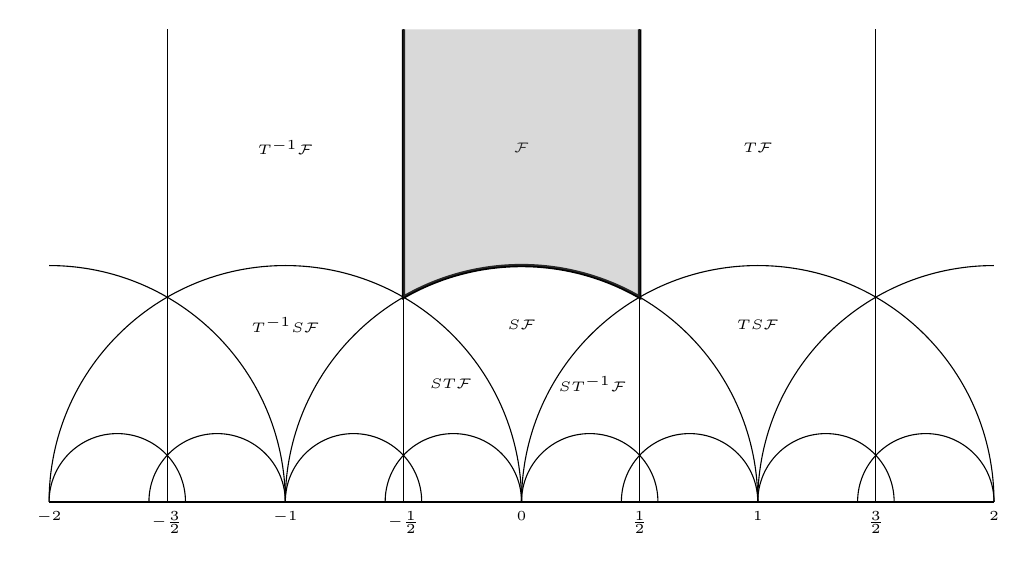
\begin{tikzpicture}[scale=3]
        \def\xmin{-2} \def\xmax{2}
        \def\ymin{0} \def\ymax{2}
        \draw[thick] (\xmin,0) -- (\xmax,0);

        \draw[very thick] (0.5,\ymax) -- (0.5,{sqrt(3)/2}) arc (60:120:1) -- (-0.5,\ymax);

        \node at (-0.5,0) [below] {\tiny{$-\frac{1}{2}$}};
        \node at (0.5,0) [below] {\tiny{$\frac{1}{2}$}};
        \node at (-1.5,0) [below] {\tiny{$-\frac{3}{2}$}};
        \node at (1.5,0) [below] {\tiny{$\frac{3}{2}$}};
        \node at (0,0) [below] {\tiny{$0$}};
        \node at (-1,0) [below] {\tiny{$-1$}};
        \node at (1,0) [below] {\tiny{$1$}};
        \node at (-2,0) [below] {\tiny{$-2$}};
        \node at (2,0) [below] {\tiny{$2$}};

        \draw[thin] (0.5,0) -- (0.5,\ymax);
        \draw[thin] (-0.5,0) -- (-0.5,\ymax);
        \draw[thin] (1.5,0) -- (1.5,\ymax);
        \draw[thin] (-1.5,0) -- (-1.5,\ymax);

        \draw (1,0) arc (0:180:1);
        \draw (-1,0) arc (0:90:1);
        \draw (2,1) arc (90:180:1);

        \draw (0,0) arc (0:180:1);
        \draw (2,0) arc (0:180:1);

        \draw (1,0) arc (0:180:{sqrt(3)/6});
        \draw ({sqrt(3)/3},0) arc (0:180:{sqrt(3)/6});

        \draw (2,0) arc (0:180:{sqrt(3)/6});
        \draw ({1+sqrt(3)/3},0) arc (0:180:{sqrt(3)/6});

        \draw (0,0) arc (0:180:{sqrt(3)/6});
        \draw ({(sqrt(3)/3)-1},0) arc (0:180:{sqrt(3)/6});

        \draw (-1,0) arc (0:180:{sqrt(3)/6});
        \draw ({(sqrt(3)/3)-2},0) arc (0:180:{sqrt(3)/6});

        \node at (0,1.5) {\tiny{$\mc{F}$}};
        \node at (-1,1.5) {\tiny{$T^{-1}\mc{F}$}};
        \node at (1,1.5) {\tiny{$T\mc{F}$}};
        \node at (0,0.75) {\tiny{$S\mc{F}$}};
        \node at (-1,0.75) {\tiny{$T^{-1}S\mc{F}$}};
        \node at (1,0.75) {\tiny{$TS\mc{F}$}};
        \node at (-0.3,0.5) {\tiny{$ST\mc{F}$}};
        \node at (0.3,0.5) {\tiny{$ST^{-1}\mc{F}$}};

        \begin{scope}
          \path[clip] (0.5,\ymax) -- (0.5,{sqrt(3)/2}) arc (60:120:1) -- (-0.5,\ymax) -- cycle;
          \fill[gray,opacity=0.3] (-0.5,0) rectangle (0.5,\ymax);
        \end{scope}
      \end{tikzpicture}
      \caption{The standard fundamental domain for $\PSL_{2}(\Z)\backslash\H$.} \label{fig:fundamental_domain_modular_group}
    \end{figure}
    
    The region $\mc{F}$, shaded in \cref{fig:fundamental_domain_modular_group}, is called the \textbf{standard fundamental domain}\index{standard fundamental domain}. \cref{fig:fundamental_domain_modular_group} also displays how this fundamental domain changes under the actions of the generators of $\PSL_{2}(\Z)$ as in \cref{prop:PSL_generator}. A fundamental domain for any other modular curve can be built from the standard fundamental domain as the following proposition shows (see \cite{kilford2015modular} for a proof):

    \begin{proposition}\label{prop:fundamental_domain_congruence_subgroup}
      Let $\G$ be any congruence subgroup. Then
      \[
        \mc{F}_{\G} = \bigcup_{\g \in \G\backslash\PSL_{2}(\Z)}\g\mc{F},
      \]
      is a fundamental domain for $\G\backslash\H$.
    \end{proposition}

    We might notice that $\mc{F}$ in \cref{fig:fundamental_domain_modular_group} is unbounded as it doesn't contain the point $\infty$. However, if we consider $\mc{F} \cup \{\infty\}$ then it would appear that this space is compact. The point $\infty$ is an example of a cusp and we now make this idea precise. Since any $\g \in \PSL_{2}(\Z)$ preserves $\hat{\R}$ and $\g$ has integer entries, $\g$ also preserves $\Q \cup \{\infty\}$. A \textbf{cusp}\index{cusp} of $\GH$ is an element of of $\G\backslash(\Q \cup \{\infty\})$. As $\G$ has finite index in the modular group, there can only be finitely many cusps and the number of cusps is at most the index of $\G$. In particular, the $\G$-orbit of $\infty$ is a cusp of $\GH$. We denote cusps by gothic characters $\mf{a},\mf{b},\mf{c},\ldots$ or by representatives of their equivalence classes. For example, we let $\infty$ denote the cusp $\G\infty$.

    \begin{remark}
      It turns out that the cusps can be represented as the points needed to make a fundamental domain $\mc{F}_{\G}$ compact as a subset of $\hat{\C}$. To see this, suppose $\mf{a}$ is a limit point of $\mc{F}_{\G}$ that does not belong to $\mc{F}_{\G}$. Then $\mf{a} \in \hat{\R}$. In the case of the standard fundamental domain $\mc{F}$, $\mf{a} = \infty$ which is a cusp. Otherwise, $\mc{F}_{\G}$ is a union of images of $\mc{F}$ by \cref{prop:fundamental_domain_congruence_subgroup} and since $\PSL_{2}(\Z)\infty = \Q \cup \{\infty\}$, we find that $\mf{a} \in \Q \cup \{\infty\}$.
    \end{remark}

    Let $\G_{\mf{a}} \le \G$ denote the stabilizer subgroup of the cusp $\mf{a}$. For the $\infty$ cusp, we can describe $\G_{\infty}$ explicitly. If $\g = \begin{psmallmatrix} a & b \\ c & d \end{psmallmatrix} \in \G$ stabilizes $\infty$ then necessarily $c = 0$ and since $\det(\g) = 1$ we must have $a = d = 1$. Therefore $\g = \begin{psmallmatrix} 1 & b \\ 0 & 1 \end{psmallmatrix}$ for some $b \in \Z$ and $\g$ acts on $\H$ by translation by $b$. Of course, not every translation is guaranteed to belong to $\G$. Letting $t$ be the smallest positive integer such that $\begin{psmallmatrix} 1 & t \\ 0 & 1 \end{psmallmatrix} \in \G$, we have $\G_{\infty} = \left\<\begin{psmallmatrix} 1 & t \\ 0 & 1 \end{psmallmatrix}\right\>$. In particular, $\G_{\infty}$ is an infinite cyclic group. We say that $\G$ is \textbf{reduced at infinity}\index{reduced at infinity} if $t = 1$ so that $\G_{\infty} = \left\<\begin{psmallmatrix} 1 & 1 \\ 0 & 1 \end{psmallmatrix}\right\>$. In particular, $\G_{1}(N)$ and $\G_{0}(N)$ are reduced at infinity.
    
    \begin{remark}
      If $\G$ is of level $N$ then $N$ is the smallest positive integer such that $\G(N) \le \G$ so that $\begin{psmallmatrix} 1 & N \\ 0 & 1 \end{psmallmatrix}$ is the minimal translation guaranteed to belong to $\G$. However, there may be smaller translations so in general $t \le N$.
    \end{remark}
    
    Moreover, for any cusp $\mf{a}$ we have that $\G_{\mf{a}}$ is also an infinite cyclic group and we denote its generator by $\g_{\mf{a}}$. To see this, if $\mf{a} = \frac{a}{c}$ with $(a,c) = 1$ is a cusp of $\GH$ not equivalent to $\infty$ then there exists an $\s_{\mf{a}} \in \PSL_{2}(\Z)$ such that $\s_{\mf{a}}\infty = \mf{a}$. Indeed, there exists integers $d$ and $b$ such that $ad-bc = 1$ by B\'ezout's identity and then $\s_{\mf{a}} = \begin{psmallmatrix} a & b \\ c & d \end{psmallmatrix}$ is such a matrix. It follows that $\G_{\mf{a}} = \s_{\mf{a}}\G_{\infty}\s_{\mf{a}}^{-1}$ and since $\G_{\infty}$ is infinite cyclic so is $\G_{\mf{a}}$. We call any matrix $\s_{\mf{a}} \in \PSL_{2}(\Z)$ satisfying 
    \[
      \s_{\mf{a}}\infty = \mf{a} \quad \text{and} \quad \s_{\mf{a}}^{-1}\g_{\mf{a}}\s_{\mf{a}} = \begin{pmatrix} 1 & t \\ 0 & 1 \end{pmatrix},
    \]
    a \textbf{scaling matrix}\index{scaling matrix} for the cusp $\mf{a}$. Note that $\s_{\mf{a}}$ is determined up to composition on the right by an element of $\G_{\infty}$. Scaling matrices are useful because they allow us to transfer information at the cusp $\mf{a}$ to the cusp at $\infty$. Let $\mf{a}$ and $\mf{b}$ be cusps of $\GH$ with scaling matrices $\s_{\mf{a}}$ and $\s_{\mf{b}}$ respectively. When investigating holomorphic forms, it will be useful to have a double coset decomposition for sets of the form $\s_{\mf{a}}^{-1}\G\s_{\mf{b}}$. This is referred to as the \textbf{Bruhat decomposition}\index{Bruhat decomposition} for $\G$:

    \begin{theorem*}[Bruhat decomposition]
      Let $\G$ be any congruence subgroup and let $\mf{a}$ and $\mf{b}$ be cusps of $\GH$ with scaling matrices $\s_{\mf{a}}$ and $\s_{\mf{b}}$ respectively. Then we have the disjoint decomposition
      \[
        \s_{\mf{a}}^{-1}\G\s_{\mf{b}} = \d_{\mf{a},\mf{b}}\W_{\infty} \cup \left(\bigcup_{\substack{c \ge 1 \\ d \tmod{c}}}\W_{d/c}\right),
      \]
      where
      \[
        \W_{\infty} = \G_{\infty}\w_{\infty} = \w_{\infty}\G_{\infty} = \G_{\infty}\w_{\infty}\G_{\infty} \quad \text{and} \quad \W_{d/c} = \G_{\infty}\w_{d/c}\G_{\infty},
      \]
      for some $\w_{\infty} = \begin{psmallmatrix} 1 & \ast \\ 0 & 1 \end{psmallmatrix} \in \s_{\mf{a}}^{-1}\G\s_{\mf{b}}$ and $\w_{d/c} = \begin{psmallmatrix} a & \ast \\ c & d \end{psmallmatrix} \in \s_{\mf{a}}^{-1}\G\s_{\mf{b}}$ with $c \ge 1$ if such a matrix exists otherwise $\W_{d/c}$ is empty. Moreover, the entries $a$ and $d$ of $\w_{d/c}$ are determined modulo $c$.
    \end{theorem*}
    \begin{proof}
      We first show that $\W_{\infty}$ is nonempty if and only if $\mf{a} = \mf{b}$. Indeed, if $\w \in \W_{\infty}$ then $\w = \s_{\mf{a}}^{-1}\g\s_{\mf{b}}$ for some $\g \in \G$. Then
      \[
        \g\mf{b} = \s_{\mf{a}}\w\s_{\mf{b}}^{-1}\mf{b} = \s_{\mf{a}}\w\infty = \s_{\mf{a}}\infty = \mf{a}.
      \]
      This shows that $\mf{a} = \mf{b}$. Conversely, suppose $\mf{a} = \mf{b}$. Then $\s_{\mf{a}}^{-1}\G\s_{\mf{b}}$ contains $\s_{\mf{a}}^{-1}\G_{\mf{a}}\s_{\mf{a}} = \G_{\infty}$ so that $\W_{\infty}$ is nonempty. So $\W_{\infty}$ is nonempty if and only if $\mf{a} = \mf{b}$. In this case, for any two elements $\w = \s_{\mf{a}}^{-1}\g\s_{\mf{a}}$ and $\w' = \s_{\mf{a}}^{-1}\g'\s_{\mf{a}}$ of $\W_{\infty}$, we have
      \[
        \g'\g^{-1}\mf{a} = \s_{\mf{a}}\w'\w^{-1}\s_{\mf{a}}^{-1}\mf{a} = \s_{\mf{a}}\w'\w^{-1}\infty = \s_{\mf{a}}\mf{a}.
      \]
      Hence $\g'\g^{-1} \in \G_{\mf{a}}$ which implies $\w'\w^{-1} = \s_{\mf{a}}^{-1}\g'\g^{-1}\s_{\mf{a}} \in \s_{\mf{a}}^{-1}\G_{\mf{a}}\s_{\mf{a}} = \G_{\infty}$. Therefore
      \[
        \W_{\infty} = \G_{\infty}\w = \w\G_{\infty} = \G_{\infty}\w\G_{\infty},
      \]
      where the latter two equalities hold because $\w$ is a translation and translations commute. Every other element of $\s_{\mf{a}}^{-1}\G\s_{\mf{b}}$ belongs to one of the double cosets $\W_{d/c}$ with $c \ge 1$ (since we are working in $\PSL_{2}(\Z)$). The relation
      \[
        \begin{pmatrix} 1 & n \\ 0 & 1 \end{pmatrix}\begin{pmatrix} a & \ast \\ c & d \end{pmatrix}\begin{pmatrix} 1 & m \\ 0 & 1 \end{pmatrix} = \begin{pmatrix} a+cn & \ast \\ c & d+cm \end{pmatrix},
      \]
      shows that $\W_{d/c}$ is determined uniquely by $c$ and $d \tmod{c}$. Moreover, this relation shows that $a$ and $d$ are determined modulo $c$. This completes the proof of the theorem.
    \end{proof}

    Notice that the Bruhat decomposition for $\s_{\mf{a}}^{-1}\G\s_{\mf{b}}$ implies
    \[
      \G_{\infty}\backslash\s_{\mf{a}}^{-1}\G\s_{\mf{b}} = \d_{\mf{a},\mf{b}}\w_{\infty} \cup \left(\bigcup_{\substack{c \ge 1 \\ d \tmod{c}}}\w_{d/c}\G_{\infty}\right),
    \]
    where it is understood that the coset $\w_{d/c}\G_{\infty}$ is empty if the double coset $\W_{d/c}$ is too. This shows that every element of $\G_{\infty}\backslash\s_{\mf{a}}^{-1}\G\s_{\mf{b}}$ corresponds to a unique $(c,d) \in \Z^{2}-\{\mathbf{0}\}$ with $c \ge 1$, $d \in \Z$, and $(c,d) = 1$, and additionally the pair $(0,1)$ if and only if $\mf{a} = \mf{b}$ (this pair corresponds to $\w_{\infty}$). Of course, this correspondence need not be surjective since many of the double cosets $\W_{d/c}$ may be empty. To track such $c$ and $d$ for which $\W_{d/c}$ is nonempty, let $\mc{C}_{\mf{a},\mf{b}}$ and $\mc{D}_{\mf{a},\mf{b}}(c)$ be the sets given by
    \[
      \mc{C}_{\mf{a},\mf{b}} = \left\{c \ge 1: \begin{pmatrix} \ast & \ast \\ c & \ast \end{pmatrix} \in \s_{\mf{a}}^{-1}\G\s_{\mf{b}}\right\} \quad \text{and} \quad \mc{D}_{\mf{a},\mf{b}}(c) = \left\{d \tmod{c}: \begin{pmatrix} \ast & \ast \\ c & d \end{pmatrix} \in \s_{\mf{a}}^{-1}\G\s_{\mf{b}}\right\}.
    \]
    Then $\mc{C}_{\mf{a},\mf{b}}$ and $\mc{D}_{\mf{a},\mf{b}}(c)$ are precisely the sets of $c$ and $d$ take modulo $c$ such that $\W_{d/c}$ is nonempty.

    \begin{remark}\label{rem:Bruhat_modulo_infity_exact}
      The Bruhat decomposition for $\s_{\mf{a}}^{-1}\G\s_{\mf{b}}$ implies
      \[
        \G_{\infty}\backslash\s_{\mf{a}}^{-1}\G\s_{\mf{b}} = \d_{\mf{a},\mf{b}}\w_{\infty} \cup \left(\bigcup_{\substack{c \in \mc{C}_{\mf{a},\mf{b}} \\ d \in \mc{D}_{\mf{a},\mf{b}}(c)}}\w_{d/c}\G_{\infty}\right),
      \]
      where none of the cosets $\w_{d/c}\G_{\infty}$ are empty. In particular, $\g = \begin{psmallmatrix} \ast & \ast \\ c & d \end{psmallmatrix} \in \G_{\infty}\backslash\s_{\mf{a}}^{-1}\G\s_{\mf{b}}$ if and only if $(c,d)$ is a pair with $c \in \mc{C}_{\mf{a},\mf{b}}$, $d \in \Z$, and $d \tmod{c} \in \mc{D}_{\mf{a},\mf{b}}(c)$, or additionally $(0,1)$ if $\mf{a} = \mf{b}$.
    \end{remark}
    
    We will now introduce Kloosterman and Sali\'e sums associated to cusps. We being with the Kloosterman sums. Let $\s_{\mf{a}}$ and $\s_{\mf{b}}$ be scaling matrices for the cusps $\mf{a}$ and $\mf{b}$ respectively. Then for any $c \in \mc{C}_{\mf{a},\mf{b}}$ and $n,m \in \Z$, the \textbf{generalized Kloosterman sum}\index{generalized Kloosterman sum} $K_{\mf{a},\mf{b}}(n,m,c)$ relative to $\mf{a}$ and $\mf{b}$ is defined by
    \[
      K_{\mf{a},\mf{b}}(n,m,c) = \sum_{d \in \mc{D}_{\mf{a},\mf{b}}(c)}e^{\frac{2\pi i(an+\conj{a}m)}{c}},
    \]
    where $a$ has been determined by $ad-bc = 1$. This sum is well-defined by the Bruhat decomposition because $a$ is determined modulo $c$. In general, $K_{\mf{a},\mf{b}}(n,m,c)$ is not independent of the scaling matrices $\s_{\mf{a}}$ and $\s_{\mf{b}}$. However, if $n = m = 0$ we trivially see by the Bruhat decomposition for $\G$ that
    \[
      K_{\mf{a},\mf{b}}(0,0,c) = \left|\left\{d \tmod{c}:\begin{pmatrix} \ast & \ast \\ c & d \end{pmatrix} \in \s_{\mf{a}}^{-1}\G\s_{\mf{b}}\right\}\right|,
    \]
    which is independent of the scaling matrices $\s_{\mf{a}}$ and $\s_{\mf{b}}$. Moreover, for $\G = \G_{1}(1)$ we have $\mf{a} = \mf{b} = \infty$ and the Bruhat decomposition for $\G_{1}(1)$ implies
    \[
      K_{\infty,\infty}(n,m,c) = K(n,m,c),
    \]
    is the usual Kloosterman sum. Therefore if $\mf{a} = \mf{b} = \infty$, we will suppress these dependencies accordingly. The Sali\'e sums are defined in a similar manner. Let $\s_{\mf{a}}$ and $\s_{\mf{b}}$ be scaling matrices for the cusps $\mf{a}$ and $\mf{b}$ respectively. Then for any $c \in \mc{C}_{\mf{a},\mf{b}}$, and $n,m \in \Z$, and Dirichlet character $\chi$ with conductor $q \mid c$, the \textbf{generalized Sali\'e sum}\index{generalized Sali\'e sum} $S_{\chi,\mf{a},\mf{b}}(n,m,c)$ relative to $\mf{a}$ and $\mf{b}$ is defined by
    \[
      S_{\chi,\mf{a},\mf{b}}(n,m,c) = \sum_{d \in \mc{D}_{\mf{a},\mf{b}}(c)}\chi(a)e^{\frac{2\pi i(an+\conj{a}m)}{c}},
    \]
    where $a$ has been determined by $ad-bc = 1$. This sum is well-defined by the Bruhat decomposition because $a$ is determined modulo $c$. Like the generalized Kloosterman sum, $S_{\mf{a},\mf{b}}(n,m,c)$ need not independent of the scaling matrices $\s_{\mf{a}}$ and $\s_{\mf{b}}$. Moreover, for $\G = \G_{1}(1)$ we have $\mf{a} = \mf{b} = \infty$ and the Bruhat decomposition for $\G_{1}(1)$ implies
    \[
      S_{\chi,\infty,\infty}(n,m,c) = S_{\chi}(n,m,c),
    \]
    is the usual Sali\'e sum. Therefore if $\mf{a} = \mf{b} = \infty$, we will suppress these dependencies accordingly.
  \section{The Hyperbolic Measure}
    We will also need to integrate over $\GH$. In order to do this, we require a measure on $\H$. Our choice of measure will be the \textbf{hyperbolic measure}\index{hyperbolic measure} $d\mu$ given by
    \[
      d\mu = d\mu(z) = \frac{dx\,dy}{y^{2}}.
    \]
    The most important property about the hyperbolic measure is that it is $\GL_{2}^{+}(\R)$-invariant (see \cite{diamond2005first} for a proof):

    \begin{proposition}
      The hyperbolic measure $d\mu$ is $\GL_{2}^{+}(\R)$-invariant.
    \end{proposition}

    As this fact will be used so frequently any time we integrate, we will not mention it explicitly. A particularly important fact is that if $\G$ is a congruence subgroup then $d\mu$ is $\G$-invariant. One of the reasons this is useful is because we can apply the unfolding/folding method to many integrals. The most common instance is when we are integrating the sum $\sum_{\g \in \GG}f(\g z)$ of some holomorphic function $f(z)$ over a fundamental domain $\mc{F}_{\G}$ for $\GH$. Indeed, $\H = \bigcup_{\g \in \G}\g\mc{F}_{\G}$ and so $\G_{\infty}\backslash\H = \bigcup_{\g \in \GG}\g\mc{F}_{\G}$. Since $\mc{F}_{\G}$ is a fundamental domain, the conditions of the unfolding/folding method are satisfied and it follows that
    \[
      \int_{\mc{F}_{\G}}\sum_{\g \in \GG}f(\g z)\,d\mu = \int_{\G_{\infty}\backslash\H}f(z)\,d\mu,
    \]
    provided either side is absolutely convergent. It is also worth highlighting another fact. Any $\a \in \GL_{2}^{+}(\Q)$ acts as an automorphism of $\H$ which implies that it induces a bijection between $\a^{-1}\G\a\backslash\H$ and $\G\backslash\H$ and hence between the fundamental domains $\mc{F}_{\a^{-1}\G\a}$ and $\mc{F}_{\G}$. Thus the change of variables $z \mapsto \a z$ transforms the fundamental domain $\mc{F}_{\G}$ into $\mc{F}_{\a^{-1}\G\a}$. Therefore
    \[
      \int_{\mc{F}_{\G}}f(z)\,d\mu = \int_{\mc{F}_{\a^{-1}\G\a}}f(\a z)\,d\mu,
    \]
    provided either side is bounded. Now let us discuss the volume of $\GH$. We define the \textbf{volume}\index{volume} $V_{\G}$ of $\GH$ by
    \[
      V_{\G} = \int_{\mc{F}_{\G}}\,d\mu.
    \]
    In other words, $V_{\G}$ is the volume of the fundamental domain $\mc{F}_{\G}$ with respect to the hyperbolic measure. Also, if $\mc{F}_{\G} = \mc{F}$ we write $V_{\G} = V$. Since the integrand is $\G$-invariant, $V_{\G}$ is independent of the choice of fundamental domain. Using \cref{prop:fundamental_domain_modular_group}, we have
    \[
      V = \int_{\mc{F}}\,d\mu = \int_{-\frac{1}{2}}^{\frac{1}{2}}\int_{\sqrt{1-x^{2}}}^{\infty}\frac{dy\,dx}{y^{2}} = \int_{-\frac{1}{2}}^{\frac{1}{2}}\frac{1}{\sqrt{1-x^{2}}}\,dx = \arcsin(x)\bigg|_{-\frac{1}{2}}^{\frac{1}{2}} = \frac{\pi}{3}.
    \]
    Therefore $V$ is finite. There is also a simple relation between $V_{\G}$ and the index of $\G$ in $\PSL_{2}(\Z)$:
    \begin{equation}\label{equ:Petersson_volume_relation}
      V_{\G} = [\PSL_{2}(\Z):\G]V,
    \end{equation}
    which follows immediately from \cref{prop:fundamental_domain_congruence_subgroup}. Moreover, $V_{\G}$ is finite for every congruence subgroup $\G$ by \cref{equ:Petersson_volume_relation} and that congruence subgroups have finite index in the modular group. A particularly nice application of this fact is that any integral of the form
    \[
      \frac{1}{V_{\G}}\int_{\mc{F}_{\G}}f(z)\,d\mu,
    \]
    is absolutely convergent provided $f(z)$ is bounded. That is, bounded functions are absolutely convergent over $\mc{F}_{\G}$ with respect to $d\mu$. Moreover, we have a useful lemma:

    \begin{lemma}\label{lem:invariance_of_volume}
      Let $\G$ be a congruence subgroup and $\a \in \GL_{2}^{+}(\Q)$. If $\a^{-1}\G\a \subseteq \PSL_{2}(\Z)$ then $V_{\a^{-1}\G\a} = V_{\G}$ and $[\PSL_{2}(\Z):\a^{-1}\G\a] = [\PSL_{2}(\Z):\G]$.
    \end{lemma}
    \begin{proof}
      The first statement follows from the chain
      \[
        V_{\a^{-1}\G\a} = \int_{\mc{F}_{\a^{-1}\G\a}}\,d\mu = \int_{\mc{F}_{\G}}\,d\mu = V_{\G},
      \]
      where the middle equality is justified by making the change of variables $z \mapsto \a^{-1}z$. The second statement is now immediate from \cref{equ:Petersson_volume_relation}.
    \end{proof}
  \chapter{Hypotheses of \texorpdfstring{$L$}{L}-functions}
  In this chapter we discuss two hypotheses of $L$-functions. The first is the more important open question in number theory and perhapse all of mathematics: the Riemann hypothesis. It discusses the distribution of the zeros of the Riemann zeta function. After surveying the Riemann hypothesis we introduce its weaker cousin the Lindel\"of hypothesis which is about the growth rate of the Riemann zeta function along the crtitical line. In our survey of the Lindel\"of hypothesis we also discuss the classical convexity argument. Analogs of these hypotheses to other $L$-functions are also mentioned.
  \section{The Riemann Hypothesis \& Nontrivial Zeros}
      Along with non-vanishing results, it turns out that the zeros of $L$-functions are also extremely important but this requires some level of discussion to be convincing. Let's start with our prototypical $L$-function the Riemann zeta function. We would like to understand its zeros. Reall that for $\Re(s) > 1$, $\z(s)$ admits an Euler product:
      \[
        \z(s) = \prod_{p}(1-p^{-s})^{-1}.
      \]
      This product vanishes if and only if one of its factors are zero. But in the region $\Re(s) > 1$, $(1-p^{-s})^{-1} \neq 0$ so $\z(s)$ has no zeros in this region. The functional equation will allow us to understand the zeros in the region $\Re(s) < 0$. Indeed, we can rewrite the functional equation for $\z(s)$ as
      \begin{equation}\label{equ:fun_eq_zeta_for_zero_type}
        \z(1-s) = \pi^{\frac{1}{2}-s}\frac{\G\left(\frac{s}{2}\right)}{\G\left(\frac{1-s}{2}\right)}\z(s).
      \end{equation}
      We want to understand when the right-hand side of \cref{equ:fun_eq_zeta_for_zero_type} vanishes in the region $\Re(s) \ge 1$. We just showed that $\z(s)$ has no zeros in the region $\Re(s) > 1$ and by \cref{thm:non-vanishing_of_zeta_on_Re(s)=1} this extends to $\Re(s) \ge 1$. So if there is a zero it comes from either of the gamma factors. This happens exactly at poles of $\G\left(\frac{1-s}{2}\right)$ for $\Re(s) \ge 1$ which by \cref{thm:continuation_of_gamma_function} are all simple and occur at $s = 1+2n$ for any integer $n \ge 0$. But at $s = 0$, $\G\left(\frac{s}{2}\right)$ has a simple pole and this cancels the simple zero of the other gamma factor. In terms of the region $\Re(s) \le 0$, $\z(s)$ has simple zeros at $s = -2n$ for $n \ge 1$. So we have shown that $\z(s)$ has simple zeros at negative even integers.

      Let $\chi$ be a primitive Dirichlet character of modulus $q > 1$. We can repeat the same procedure for $L(s,\chi)$. Indeed, for $\Re(s) > 1$, $L(s,\chi)$ has the Euler product
      \[
        L(s,\chi) = \prod_{p}(1-\chi(p)p^{-s})^{-1},
      \]
      and this product vanishes if and only if one of the factors are zero. But for $\Re(s) > 1$, $(1-\chi(p)p^{-s})^{-1} \neq 0$ so $L(s,\chi)$ has no zeros in this region. We can rewrite the functional equation for $L(s,\chi)$ as
      \begin{equation}\label{equ:fun_eq_Dirichlet_for_zero_type}
        L(1-s,\chi) = \frac{i^{\mf{a}}}{\e_{\chi}}q^{s-\frac{1}{2}}\pi^{s-\frac{1}{2}}\frac{\G\left(\frac{s+\mf{a}}{2}\right)}{\G\left(\frac{(1-s)+\mf{a}}{2}\right)}L(s,\cchi).
      \end{equation}
      Just as for $\z(s)$, we want to understand when the right-hand side of \cref{equ:fun_eq_Dirichlet_for_zero_type} vanishes for $\Re(s) \ge 1$. Now $L(s,\chi)$ and $L(s,\cchi)$ don't have zeros in the region $\Re(s) > 1$ and by \cref{thm:non-vanishing_of_Dirichlet_on_Re(s)=1} this extends to $\Re(s) \ge 1$. Hence the right-hand side is zero if and only if one of the gamma factors vanish. The zeros come from the poles of $\G\left(\frac{(1-s)+\mf{a}}{2}\right)$ for $\Re(s) \ge 1$. By \cref{thm:continuation_of_gamma_function} these are all simple and occur at $s = 1+\mf{a}+2n$ for $n \ge 0$. In terms of the region $\Re(s) \le 0$, $L(s,\chi)$ has simple zeros at $s = -2n$ for $n \ge 0$ if $\chi$ is even and at $s = -(2n+1)$ for $n \ge 0$ if $\chi$ is odd. We can state our results compactly as follows: $L(s,\chi)$ has simple zeros at nonpositive even integers if $\chi$ is even and at negative odd integers if $\chi$ is odd. In particular, if $\chi$ is even there is a zero at $s = 0$ (a boundary point of the critical strip).

      For a general Selberg class $L$-function $L(s)$, the situation is analogous. From the Euler product, $L(s)$ will have no zeros in the region $\Re(s) > 1$. The functional equation then shows that the zeros $L(s)$ in the region $\Re(s) < 0$ come from the the poles of the gamma functions. Some additional care is needed at the boundary lines $\Re(s) = 0,1$. The zeros of $L(s)$ outside or at the boundary of the critial strip are called \textbf{trivial zeros}\index{trivial zeros}. The zeros of $L(s)$ inside the critical strip are called \textbf{nontrivial zeros}\index{nontrivial zeros}.

      Returning to the Riemann zeta function, let $\rho$ be a nontrivial zero. Inside the critial strip the gamma factors in the functional equation are holomorphic and non-vanishing. So the functional equation implies $1-\rho$ is also a nontrivial zero. Actually, we can do slighly better. Since $\z(s)$ takes real values for real $s > 1$ ($\z(s)$ is defined by a Dirichlet series there), the Schwarz reflection principle implies $\z(\conj{s}) = \conj{\z(s)}$ and that $\z(s)$ takes real values on the entire real axis (save for the pole). So $\conj{\rho}$ and $1-\conj{\rho}$ are nontrivial zeros too and therefore the nontrivial zeros of $z(s)$ come in sets of four:
      \[
        \rho, \quad \conj{\rho}, \quad 1-\rho, \quad \text{and} \quad 1-\conj{\rho}.
      \]
      Almost the same type of symmetry holds for $L(s,\chi)$. Let $\rho$ be a nontrivial zero of $L(s,\chi)$. Note that $\conj{L(s,\chi)} = L(\conj{s},\cchi)$ by the identity theorem and that this equality holds for $\Re(s) > 1$ (where $L(s,\chi)$ is defined by a Dirichlet series). This implies $\conj{\rho}$ is a nontrivial zero of $L(s,\cchi)$. Inside the critical strip, the gamma factors in the functional equation are nonzero and holomorphic so we conclude that $1-\conj{\rho}$ is also a nontrivial zero of $L(s,\chi)$. Unfortunately, if $\chi$ is complex $L(s,\chi)$ does not necessarily take real values for real $s > 1$ and so we cannot conclude that $\conj{\rho}$ is a nontrivial zero. However, if $\chi$ is quadratic then it only takes real values and so $\conj{\rho}$ will also be a nontrivial zero. In the case of $\z(s)$, the Riemann hypothesis says that this symmetry of zeros is as simple as it could possibly be:

      \begin{theorem}[Riemann hypothesis]
        All of the nontrivial zeros of $\z(s)$ lie on the line $\Re(s) = \frac{1}{2}$.
      \end{theorem}

      This is one of, if not the most, famous and important open problems in mathematics. It has resisted all attempts of a proof by every great mathematician over the last century and a half. The Clay Mathematics Institute has also named it one of the millennium pize problems which means that anyone who can give a proof (or disproof) will recieve a \$1 million cash prize. Riemann's original motivation for the conjecture came from looking for an explicit formula for $\pi(x)$ which is the purpose of his 1859 manuscript (see \cite{riemann1859ueber}). This explicit formula for $\pi(x)$ involves the nontrivial zeros of Riemann zeta function. Riemann computed a few of them, found that they were on the critical line, and conjectured that it is very likely that all of them lie on the critical line.

      The Riemann hypothesis is important because, if true, it tells us a lot of information about how the primes are distributed among the positive integers. In particular, Koch in 1901 showed that the Riemann hypothesis implies an asymptotic estimate for the exact error between $\pi(x)$ and $\Li(x)$ (see \cite{von1901distribution}):

      \begin{proposition}
        Under the assumption of the Riemann hypothesis,
        \[
          \pi(x) = \Li(x)+O(\sqrt{x}\log(x)).
        \]
      \end{proposition}

      The Riemann hypothesis also implies the Lindel\"of hypothesis although it is not an immediate consequence. In 1919 Backlund showed the following equivalence for the Lindel\"of hypothesis (see \cite{backlund1919beziehung}):

      \begin{proposition}\label{prop:Lindelof_hypothesis_equivalence}
      The Lindel\"of hypothesis is equivalent to the following statement: Fix an $\e > 0$, a real $T$, and set
      \[
        Z_{\e,T} = \left\{s \in \C : \z(s) = 0, \Re(s) \ge \frac{1}{2}+\e, T \le \Im(s) \le T+1 \right\}.
      \]
      Then
      \[
        |Z_{\e,T}| = o(\log(T)).
      \]
      \end{proposition}

      If the Riemann hypothesis is true, then \cref{prop:Lindelof_hypothesis_equivalence} is immediate because $Z_{\e,T}$ would be empty for any $\e > 0$ and all $T$. Therefore the Riemann hypothesis implies the Lindel\"of hypothesis. There are more interesting implications and consequences but we will not discuss them here. Instead, we would like to make an interesting comment about \cref{thm:Littlewood_Li_approximation_theorem}. The original proof (see \cite{hardy1916contributions}) is actually independent of the truth of the Riemann hypothesis. Assuming the Riemann hypothesis is true, one deduces a contradiction if $\pi-\Li(x)$ changes sign finitely many times. Then assuming the Riemann hypothesis is false, one again deduces a contradiction if $\pi-\Li(x)$ changes sign finitely many times.

      Lastly, there is also the \textbf{Selberg class Riemann hypothesis}\index{Selberg class Riemann hypothesis} which is an analogous conjecture for Selberg class $L$-functions:

      \begin{conjecture}[Selberg class Riemann hypothesis]
        For any Selberg class $L$-function $L(s)$, all of the nontrivial zeros of $L(s)$ lie on the line $\Re(s) = \frac{1}{2}$.
      \end{conjecture}

      The Selberg class Riemann hypothesis also implies other interesting results, but we will not discuss them here.
  \section{The Lindel\"of Hypothesis \& Convexity Arguments}
    A slightly weaker conjectured result than the Riemann hypothesis is the Lindel\"of hypothesis. In 1908 Lindel\"of made a conjecture which is about the rate of growth of the zeta function on the critical line (see \cite{lindelof1908quelques}). This is now known as the \textbf{classical Lindel\"of hypothesis}\index{classical Lindel\"of hypothesis}:

    \begin{conjecture}[Classical Lindel\"of hypothesis]
      For any $\e > 0$,
      \[
        \z\left(\frac{1}{2}+it\right) \ll_{\e} t^{\e}.
      \]
    \end{conjecture}

    This conjecture still remains wide open today, but over the years there have been some advances toward proving this conjecture. These advances go by the name of subconvexity arguments. This motivates the question: what is a convexity argument anways? A \textbf{convexity argument}\index{convexity argument} is one where estimates about the growth of an $L$-function on the critical line is dervied from \textbf{trivial bounds}\index{trivial bounds}, that is bounds given by absolute convergence, via the functional equation. Usually this is achieved by methods of complex analysis and Sirling's formula.

    We will demonstrate a standard convexity argument, also referred to as the \textbf{Lindel\"of convexity argument}\index{Lindel\"of convexity argument} for the Riemann zeta function. Let $s = \s+it$. The first step is to guarantee the Phragm\'en-Lindel\"of convexity principle in a region containing the critical strip. The zeta function being order $1$ implies this immediately (see \cref{append:The_Phragmen_Lindelof_Convexity_principle}). Therefore, we are reduced to estimating the growth of $\z(s,f)$ for $\s$ to the left of $0$ and to the right of $1$. That is, just outside the edges of the critical strip. The right edge is easy. Letting $\e > 0$ and setting $\s = 1+\e$, we have that the zeta function is absolutely convergent in this region giving the trivial bound
    \begin{equation}\label{equ:convexity_bound_1}
      \z((1+\e)+it,f) \ll_{\e} 1.
    \end{equation}
    The left edge is only slightly more difficult. The functional equation implies
    \begin{equation}\label{equ:convexity_bound_left_edge}
      |\z(s,f)| \le \left|\frac{\g(1-s,f)}{\g(s,f)}\right||\z(1-s,f)|.
    \end{equation}
    We now require an estimate for the ratio of the gamma factors. We will get this estimate from \cref{equ:weaker_Stirling_formula}. Since $s \sim_{\s} t$, we replace $s$ with $t$, except for the exponenets, provided we let the implicit constant depend upon $\s$. For the exponents, we can reaplce $s$ with $\s$ because any complex number raised to a purely imaginary power has absolute value $1$. So, our simplified estimate is
    \[
      \G(s) = \sqrt{2\pi}t^{\s-\frac{1}{2}}e^{-\s}(1+O_{\s}(1)),
    \]
    which is equivalent to
    \[
      \frac{1}{\G(s)} = \frac{1}{\sqrt{2\pi}}t^{\frac{1}{2}-\s}e^{\s}(1+O_{\s}(1)),
    \]
    In terms of Vinogradov's symbol the above estimates imply
    \[
      \G(s) \ll_{\s} t^{\s-\frac{1}{2}}e^{-\s} \ll_{\s} t^{\s-\frac{1}{2}} \quad \text{and} \quad \frac{1}{\G(s)} \ll_{\s} t^{\frac{1}{2}-\s}e^{\s} \ll_{\s} t^{\frac{1}{2}-\s}.
    \]
    We can then estimate the ratio of gamma factors as 
    \begin{equation}\label{equ:ratio_of_gamma_estimate}
      \frac{\G(1-s)}{\G(s)} \ll_{\s} t^{1-2\s}.
    \end{equation}

    From \cref{equ:ratio_of_gamma_estimate} it follows that
    \[
      \frac{\g(1-s,f)}{\g(s,f)} \ll_{\s} t^{\frac{1-2\s}{2}}.
    \]
    Let $\e > 0$ and set $\s = -\e$. Then plugging our estimate above into \cref{equ:convexity_bound_left_edge} and using the trivial bound $|\z((1+\e)+it)| \ll_{\e} 1$ gives
    \begin{equation}\label{equ:convexity_bound_2}
      \z(-\e+it) \ll_{\e} t^{\frac{1+2\e}{2}}.
    \end{equation}
    By the Phragm\'en-Lindel\"of convexity principle, \cref{equ:convexity_bound_1,equ:convexity_bound_2} imply the \textbf{convexity bound}\index{convexity bound}
    \[
      \z(s) \ll_{\s,\e} t^{\frac{1+\e-\s}{2}},
    \]
    for $-\e \le \s \le 1+\e$. At the critical line, the convexity bound becomes
    \begin{equation}\label{equ:convexity_bound_zeta_function}
      \z\left(\frac{1}{2}+it\right) \ll_{\e} t^{\frac{1}{4}+\e}.
    \end{equation}
    So the classical Lindel\"of hypothesis says that the exponenet $\frac{1}{4}+\e$ can be improved to be $\e$. For a general Selberg class $L$-function, the Lindel\"of convexity argument is the following:

    \begin{method}[Lindel\"of convexity argument]
      Suppose we are given a general $L$-function $L(s,f)$ with degree $d$ Euler product (not necessarily of the Selberg class) and such that the following hold:
      \begin{enumerate}[label=(\roman*)]
        \item $L(s,f)$ is absolutely convergent for $\Re(s) > 1$.
        \item $L(s,f)$ has a functional equation of shape $s \to 1-s$ with conductor $q(f)$.
        \item $L(s,f)$ is of finite order.
        \item $L(s,f)$ has analytic continuation to the critical strip.
      \end{enumerate}
      Then the \textbf{convexity bound}\index{convexity bound}
      \[
        L(s,f) \ll_{\s,\e} q(f)^{\frac{1+\e-\s}{2}}t^{\frac{d(1+\e-\s)}{2}},
      \]
      can be obtained inside the critical strip. Indeed, if $L(s)$ has poles inside the critical strip, remove them by multiplying by the corresponding polar divisors. We can then divide out by these factors after obtaining the estimate. Since $L(s)$ is finite order, $L(s)$ will satisfy the Phragm\'en-Lindel\"of convexity principle in a region containing the critical strip. Now use the absolute convergence of $L(s)$ to bound the right edge by a constant. Then use the functional equation to isolate the $L$-function at the left edge and apply Stirling's formula to the ratio of gamma factors coming from the functional equation to deduce a polynomial bound of shape $q(f)^{\frac{1+2\e}{2}}t^{\frac{d(1+2\e)}{2}}$. The Phragm\'en-Lindel\"of convexity principle will then give the result.
    \end{method}

    Notice that the convexity bound depends on the degree $d$ of the Euler product and the conductor $q(f)$ (for the Riemann zeta function the conductor is $1$). In particular, at the critical line the Lindel\"of convexity argument gives a polynomials bound of $\frac{d}{4}+\e$ in $t$ and $\frac{1}{4}+\e$ in $q(f)$. The polynomial bound in $t$ depends upon $d$ because there is one gamma function in the gamma factor for each degree of the Euler product. For any such $L$-function, any improvment upon either exponent at the critical line is called \textbf{breaking convexity}\index{breaking convexity} and any argument used to do so is called a \textbf{subconvexity argument}\index{subconvexity argument}. Often, we refer to the \textbf{$t$-aspect}\index{$t$-aspect} (or \textbf{height aspect}\index{height aspect}) to mean the polynomial bound in $t$. Similarly, we refer to the \textbf{$q(f)$-aspect}\index{$q(f)$-aspect} (or \textbf{conductor aspect}\index{conductor aspect}) to mean the polynomial bound in $q(f)$. Lastly, we refer to the \textbf{hybrid aspect}\index{hybrid aspect} to mean the combined polynomial bound in $t$ and $q(f)$. For example, from the Lindel\"of convexity argument we have the convexity bound
    \[
      L\left(\frac{1}{2}+it,\chi\right) \ll_{t,\e} q^{\frac{1}{4}+\e},
    \]
    in the $q$-aspect, for any primitive Dirichlet $L$-function of conductor $q > 1$. The Lindel\"of hypothesis in the $q$-aspect for Dirichlet $L$-functions is that this exponent can be improved to be $\e$:

    \begin{conjecture}[Lindel\"of hypothesis for Dirichlet $L$-functions, $q$-aspect]
      For any \\ primitive Dirichlet character of conductor $q > 1$ and any $\e > 0$,
      \[
        L\left(\frac{1}{2}+it,\chi\right) \ll_{t,\e} q^{\e}.
      \]
    \end{conjecture}
    
     The \textbf{Selberg class Lindel\"of hypothesis}\index{Lindel\"of hypothesis} is the analog to the classical Lindel\"of hypothesis for any Selberg class $L$-function:

    \begin{conjecture}[Selberg class Lindel\"of hypothesis]
      For any Selberg class $L$-function $L(s,f)$ of conductor $q(f)$ and any $\e > 0$,
      \[
        L\left(\frac{1}{2}+it\right) \ll_{\e} (q(f)t)^{\e}.
      \]
    \end{conjecture}
  \chapter{Classical Applications}
  We will discuss some classical applications of $L$-functions. Our first result is a crowning gem of analytic number theory: Dirichlet's theorem. This result is a consequence of a non-vanishing result for Dirichlet $L$-series at $s = 1$. Then we discuss Siegel zeros in the case of Dirichlet $L$-functions and as a result obtain a lower bound for Dirichlet $L$-functions at $s = 1$. Lastly, we prove the prime number theorem and its variant for primes restricted to a certain residue class, the Siegel–Walfisz theorem, in the classical manner.
  \section{Dirichlet's Theorem}
    One of the more well-known arithmetic results proved using $L$-series is \textbf{Dirichlet's theorem}\index{Dirichlet's theorem}:

    \begin{theorem}[Dirichlet's theorem]\label{thm:Dirichlet's_theorem_on_primes_in_arithmetic_progressions}
      Let $a$ and $m$ be positive integers such that $(a,m) = 1$. Then the arithmetic progression $\{a+km \mid k \in \N\}$ contain infinitely many primes.
    \end{theorem}

    We will delay the proof for the moment, for it is well-worth understanding the some of the motivation behind why this theorem is interesting and how exactly Dirichlet used the analytic techniques of $L$-series to attack this purely arithmetic statement. We being by recalling Euclid's famous theorem on the infinitude of the primes. Euclid's proof is completely elementary and arithmetic in nature. He argues that if there were finitely many primes $p_{1},p_{2},\ldots,p_{k}$ then a short consideration of $(p_{1}p_{2} \cdots p_{k})+1$ shows that this number must either be divisible by a prime not in our list or must be prime itself. As primes are the multiplicative building blocks of arithmetic, Euclid assures us that we have an ample amount of primes to work with. Now there is a slightly stronger result due to Euler (see \cite{euler1744variae}) requiring analytic techniques:

    \begin{theorem}\label{thm:reciprocial_sum_of_primes_diverges}
      The series
      \[
        \sum_{p}\frac{1}{p},
      \]
      diverges.
    \end{theorem}
    \begin{proof}
      For $\s > 1$, taking the logarithm of the Euler product of $\z(s)$, we get
      \[
        \log\z(s) = -\sum_{p}\log(1-p^{-s}).
      \]
      The Taylor series of the logarithm gives
      \[
        \log(1-p^{-s}) = \sum_{k \ge 1}(-1)^{k-1}\frac{(-p^{-s})^{k}}{k} = \sum_{k \ge 1}(-1)^{2k-1}\frac{1}{kp^{ks}},
      \]
      so that
      \[
        \log\z(s) = \sum_{p}\sum_{k \ge 1}\frac{1}{kp^{ks}}.
      \]
      The double sum restricted to $k \ge 2$ is uniformly bounded for $\s > 1$. To see this, first observe
      \[
        \sum_{k \ge 2}\frac{1}{kp^{ks}} \ll \sum_{k \ge 2}\frac{1}{p^{k}} = \frac{1}{p^{2}}\sum_{k \ge 0}\frac{1}{p^{k}} = \frac{1}{p^{2}}(1-p^{-1})^{-1} \le \frac{2}{p^{2}},
      \]
      where the last inequality follows because $p \ge 2$. Then
      \[
       \sum_{p}\sum_{k \ge 2}\frac{1}{kp^{ks}} \ll 2\sum_{p}\frac{1}{p^{2}} < 2\sum_{n \ge 1}\frac{1}{n^{2}} = 2\z(2).
      \]
      Therefore
      \[
        \log\z(s)-\sum_{p}\frac{1}{p^{s}} = \sum_{p}\sum_{k \ge 2}\frac{1}{kp^{ks}},
      \]
      and remains bounded as $s \to 1$. The claim now follows since $\z(s)$ has a simple pole at $s = 1$.
    \end{proof}

    \cref{thm:reciprocial_sum_of_primes_diverges} tells us that there are infinitely many primes but also that the primes are not too sparse in the integers for otherwise the series would converge. The idea Dirichlet used to prove his result on primes in arithmetic progressions was in a very similar spirit. He sought out to prove the divergence of the series
    \[
      \sum_{p \equiv a \tmod{m}}\frac{1}{p},
    \]
    for positive integers $a$ and $m$ with $(a,m) = 1$ as the divergence immediately implies there are infinitely many primes $p$ of the form $p \equiv a \tmod{m}$. In the case $a = 1$ and $m = 2$ we recover \cref{thm:reciprocial_sum_of_primes_diverges} exactly since every prime is odd. Dirichlet's proof proceeds in a similar way to that of \cref{thm:reciprocial_sum_of_primes_diverges} and this is where Dirichlet used what are now known as Dirichlet characters and Dirichlet $L$-series. The proof can be broken into three steps. The first is to proceed as Euler did, but with the Dirichlet $L$-series $L(s,\chi)$ where $\chi$ has modulus $m$. That is, write $L(s,\chi)$ as a sum over primes and a bounded term as $s \to 1$. The next step is to use the orthogonality relations of the characters to sieve out the correct sum. The last step is to show the non-vanishing result $L(1,\chi) \neq 0$ for all non-principal characters $\chi$. This is the essential part of the proof as it is what assures us that the sum diverges. Luckily, we have done most of the hard work to prove this already:

    \begin{theorem}\label{thm:non-vanishing_of_Dirichlet_L-functions_at_s=1}
      Let $\chi$ be a non-principal Dirichlet character. Then $L(1,\chi)$ is finite and nonzero.
    \end{theorem}
    \begin{proof}
      This follows immediately by applying \cref{lem:non-vanshing_at_1_lemma} to $\z(s)L(s,\chi)$ and noting that $L(s,\chi)$ is holomorphic.
    \end{proof}

     We now prove Dirichlet's theorem:

    \begin{proof}[Proof of Dirichlet's theorem]
        Let $\chi$ be a Dirichlet character modulo $m$. Then for $\s > 1$, taking the logarithm of the Euler product of $L(s,\chi)$ gives
        \[
          \log{L(s,\chi)} = -\sum_{p}\log(1-\chi(p)p^{-s}).
        \]
        The Taylor series of the logarithm implies
        \[
          \log(1-\chi(p)p^{-s}) = \sum_{k \ge 1}(-1)^{k-1}\frac{(-\chi(p)p^{-s})^{k}}{k} = \sum_{k \ge 1}(-1)^{2k-1}\frac{\chi(p^{k})}{kp^{ks}},
        \]
        so that
        \[
          \log{L(s,\chi)} = \sum_{p}\sum_{k \ge 1}\frac{\chi(p^{k})}{kp^{ks}}.
        \]
        The double sum restricted to $k \ge 2$ is uniformly bounded for $\s > 1$. Indeed, first observe
        \[
          \left|\sum_{k \ge 2}\frac{\chi(p^{k})}{kp^{ks}}\right| \ll \sum_{k \ge 2}\frac{1}{p^{k}} = \frac{1}{p^{2}}\sum_{k \ge 0}\frac{1}{p^{k}} = \frac{1}{p^{2}}(1-p^{-1})^{-1} \le \frac{2}{p^{2}},
        \]
        where the last inequality follows because $p > 2$. Then
        \[
          \left|\sum_{p}\sum_{k \ge 2}\frac{\chi(p^{k})}{kp^{ks}}\right| \le 2\sum_{p}\frac{1}{p^{2}} < 2\sum_{n \ge 1}\frac{1}{n^{2}} = 2\z(2),
        \]
        as desired. Now write
        \[
          \sum_{\chi \tmod{m}}\conj{\chi(a)}\log{L(s,\chi)} = \sum_{\chi \tmod{m}}\sum_{p}\frac{\conj{\chi(a)}\chi(p)}{p^{s}}+\sum_{\chi \tmod{m}}\conj{\chi(a)}\sum_{p}\sum_{k \ge 2}\frac{\chi(p^{k})}{kp^{ks}}.
        \]
        By the orthogonality relations (\cref{prop:Dirichlet_orthogonality_relations} (ii)), we find that
        \[
          \sum_{\chi \tmod{m}}\sum_{p}\frac{\conj{\chi(a)}\chi(p)}{p^{s}} = \sum_{p}\frac1{p^{s}}\sum_{\chi \tmod{m}}\conj{\chi(a)}\chi(p) = \vphi(m)\sum_{p \equiv{a} \tmod{m}}\frac{1}{p^{s}},
        \]
        and so
        \[
          \sum_{\chi \tmod{m}}\conj{\chi(a)}\log{L(s,\chi)}-\sum_{\chi \tmod{m}}\conj{\chi(a)}\sum_{p}\sum_{k \ge 2}\frac{\chi(p^{k})}{kp^{ks}} = \vphi(m)\sum_{p \equiv{a} \tmod{m}}\frac{1}{p^{s}}.
        \]
        The triple sum is uniformly bounded for $\s > 1$ because the inner double sum is and there are finitely many Dirichlet characters modulo $m$. Therefore it suffices to show that the first sum on the left-hand side diverges as $s \to 1$. For $\chi = \chi_{m,0}$,
        \[
          L(s,\chi_{m,0}) = \z(s)\prod_{p \mid m}(1-p^{-s}),
        \]
        so the corresponding term in the sum is
        \[
          \conj{\chi_{m,0}}(a)\log L(s,\chi_{m,0}) = \log\z(s)+\sum_{p \mid m}\log(1-p^{-s}),
        \]
        which diverges as $s \to 1$ because $\z(s)$ has a simple pole at $s = 1$. We will be done if $\log{L(s,\chi)}$ remains bounded as $s \to 1$ for all $\chi \neq \chi_{m,0}$. So assume $\chi$ is non-principal. Then we must show $L(1,\chi)$ is finite and nonzero. This follows from \cref{thm:non-vanishing_of_Dirichlet_L-functions_at_s=1}.
    \end{proof}

    For primitive $\chi$ of conductor $q > 1$, we know from \cref{thm:non-vanishing_of_Dirichlet_L-functions_at_s=1} that $L(1,\chi)$ is finite and nonzero. It is interesting to know whether or not this value is computable in general. Indeed it is. The computation is fairly straightforward and only requires some basic properties of Ramanujan and Gauss sums that we have already developed. The idea is to rewrite the character values $\chi(n)$ so that we can collapse the infinite series into a Taylor series. Our result is the following:
    
    \begin{theorem}\label{thm:Value_of_Dirichlet_L-functions_at_s=1}
      Let $\chi$ be a primitive Dirichlet character with conductor $q > 1$. Then
      \[
        L(1,\chi) = -\frac{\tau(\chi)}{q}\sum_{a \tmod{q}}\cchi(a)\log\left(\sin\left(\frac{\pi a}{q}\right)\right) \quad \text{or} \quad L(1,\chi) = \frac{\tau(\chi)\pi i}{q^{2}}\sum_{a \tmod{q}}\cchi(a)a,
      \]
      according to whether $\chi$ is even or odd.
    \end{theorem}
    \begin{proof}
      First compute
      \begin{align*}
        \chi(n) &= \frac{1}{\tau(\cchi)}\sum_{a \tmod{q}}\cchi(a)e^{\frac{2\pi ian}{q}} && \text{\cref{cor:gauss_sum_primitive_formula}} \\
        &= \frac{\chi(-1)}{\conj{\tau(\chi)}}\sum_{a \tmod{q}}\cchi(a)e^{\frac{2\pi ian}{q}} && \text{\cref{prop:Gauss_sum_reduction} (i) and $\chi(-1)^{2} = 1$} \\
        &= \frac{\chi(-1)\tau(\chi)}{\tau(\chi)\conj{\tau(\chi)}}\sum_{a \tmod{q}}\cchi(a)e^{\frac{2\pi ian}{q}} \\
        &= \frac{\chi(-1)\tau(\chi)}{q}\sum_{a \tmod{q}}\cchi(a)e^{\frac{2\pi ian}{q}} && \text{\cref{thm:Gauss_sum_modulus}} \\
        &= \frac{\chi(-1)\tau(\chi)}{q}\sum_{a \tmod{q}}\cchi(a)e^{\frac{2\pi ian}{q}}.
      \end{align*}
      Substituting this result into the definition of $L(1,\chi)$, we find that
      \begin{equation}\label{equ:value_of_Dirichlet_L-functions_at_s=1_1}
        \begin{aligned}
          L(1,\chi) &= \sum_{n \ge 1}\frac{1}{n}\left(\frac{\chi(-1)\tau(\chi)}{q}\sum_{a \tmod{q}}\cchi(a)e^{\frac{2\pi ian}{q}}\right) \\
          &= \frac{\chi(-1)\tau(\chi)}{q}\sum_{a \tmod{q}}\cchi(a)\sum_{n \ge 1}\frac{e^{\frac{2\pi ian}{q}}}{n} \\
          &= \frac{\chi(-1)\tau(\chi)}{q}\sum_{a \tmod{q}}\cchi(a)\log\left(\left(1-e^{\frac{2\pi ia}{q}}\right)^{-1}\right),
        \end{aligned}
      \end{equation}
      where in the last line we have used the Taylor series of the logarithm. We will now simplify the last expression in \cref{equ:value_of_Dirichlet_L-functions_at_s=1_1}. Since $\sin(\t) = \frac{e^{i\t}-e^{-i\t}}{2i}$, we have
      \[
        1-e^{\frac{2\pi ia}{q}} = -2ie^{\frac{\pi ia}{q}}\left(\frac{e^{\frac{\pi ia}{q}}-e^{-\frac{\pi ia}{q}}}{2i}\right) = -2ie^{\frac{\pi ia}{q}}\sin\left(\frac{\pi a}{q}\right).
      \]
      Therefore the last expression in \cref{equ:value_of_Dirichlet_L-functions_at_s=1_1} becomes
      \[
        \frac{\chi(-1)\tau(\chi)}{q}\sum_{a \tmod{q}}\cchi(a)\log\left(\left(-2ie^{\frac{\pi ia}{q}}\sin\left(\frac{\pi a}{q}\right)\right)^{-1}\right).
      \]
      As $a$ is taken modulo $q$, we have $0 < \frac{\pi a}{q} < \pi$ so that $\sin\left(\frac{\pi a}{q}\right)$ is never negative. Therefore we can split up the logarithm term and obtain
      \[
        -\frac{\chi(-1)\tau(\chi)}{q}\left(\log(-2i)\sum_{a \tmod{q}}\cchi(a)+\frac{\pi i}{q}\sum_{a \tmod{q}}\cchi(a)a+\sum_{a \tmod{q}}\cchi(a)\log\left(\sin\left(\frac{\pi a}{q}\right)\right)\right).
      \]
      By the orthogonality relations (\cref{cor:Dirichlet_orthogonality_relations} (i)), the first sum above vanishes. Therefore
      \begin{equation}\label{equ:value_of_Dirichlet_L-functions_at_s=1_2}
        L(1,\chi) = -\frac{\chi(-1)\tau(\chi)}{q}\left(\frac{\pi i}{q}\sum_{a \tmod{q}}\chi(a)a+\sum_{a \tmod{q}}\chi(a)\log\left(\sin\left(\frac{\pi a}{q}\right)\right)\right).
      \end{equation}
      \cref{equ:value_of_Dirichlet_L-functions_at_s=1_2} simplifies in that one of the two sums vanish depending on if $\chi$ is even or odd. For the first sum in \cref{equ:value_of_Dirichlet_L-functions_at_s=1_2}, observe that
      \[
        \frac{\pi i}{q}\sum_{a \tmod{q}}\chi(a)a = -\frac{\chi(-1)\pi i}{q}\sum_{a \tmod{q}}\chi(-a)(-a).
      \]
      As $a \to -a$ is a bijection on $\Z/q\Z$, this sum vanishes if $\chi$ is even. For the second sum in \cref{equ:value_of_Dirichlet_L-functions_at_s=1_2}, we have an analogous relation of the form
      \[
        \sum_{a \tmod{q}}\chi(a)\log\left(\sin\left(\frac{\pi a}{q}\right)\right) = \chi(-1)\sum_{a \tmod{q}}\chi(-a)\log\left(\sin\left(\frac{\pi a}{q}\right)\right).
      \]
      As $a \to -a$ is a bijection on $\Z/q\Z$, this sum vanishes if $\chi$ is odd. This finishes the proof.
    \end{proof}

    \cref{thm:Value_of_Dirichlet_L-functions_at_s=1} encodes some interesting identities. For example, if $\chi$ is the non-principal Dirichlet character modulo $4$, then $\chi$ is uniquely defined by $\chi(1) = 1$ and $\chi(3) = \chi(-1) = -1$. In particular, $\chi$ is odd and its conductor is $4$. Now
    \[
      \tau(\chi) = \sum_{a \tmod{4}}\chi(a)e^{\frac{2\pi ia}{4}} = e^{\frac{2\pi i}{4}}-e^{\frac{6\pi i}{4}} = i-(-i) = 2i,
    \]
    so by \cref{thm:Value_of_Dirichlet_L-functions_at_s=1} we get
    \[
      L(1,\chi) = -\frac{\chi(-1)\tau(\chi)\pi i}{16}(1-3) = \frac{\pi}{4}.
    \]
    Expanding out $L(1,\chi)$ gives
    \[
      1-\frac{1}{3}+\frac{1}{5}-\frac{1}{7}+\cdots = \frac{\pi}{4},
    \]
    which is the famous \textbf{Madhava–Leibniz formula}\index{Madhava–Leibniz formula} for $\pi$.
  \section{\todo{The Analytic Class Number Formula}}
  \section{Siegel's Theorem}
    The discussion of Siegel zeros first arose during the study of zero-free regions for Dirichlet $L$-functions. Refining the argument used in \cref{thm:zero_free_region_generic}, we can show that Siegel zeros only exist when the character $\chi$ is quadratic. But first we improve the zero-free region for the Riemann zeta function:

    \begin{theorem}\label{thm:improved_zero-free_region_zeta}
      There exists a constant $c > 0$ such that $\z(s)$ has no zeros in the region
      \[
        \s \ge 1-\frac{c}{\log(|t|+3)}.
      \]
    \end{theorem}
    \begin{proof}
      By \cref{thm:zero_free_region_generic} applied to $\z(s)$, it suffices to show that $\z(s)$ has no real nontrivial zeros. To see this, let $\eta(s)$ be defined by
      \[
        \eta(s) = \sum_{n \ge 1}\frac{(-1)^{n-1}}{n^{s}}.
      \]
      Note that $\eta(s)$ converges for $\s > 0$ by \cref{prop:Dirichlet_series_convergence_bounded_coefficient_sum}. Now for $0 < s < 1$ and even $n$, $\frac{1}{n^{s}}-\frac{1}{(n+1)^{s}} > 0$ so that $\eta(s) > 0$. But for $\s > 0$, we have
      \[
        (1-2^{1-s})\z(s) = \sum_{n \ge 1}\frac{1}{n^{s}}-2\sum_{n \ge 1}\frac{1}{(2n)^{s}} = \sum_{n \ge 1}\frac{(-1)^{n-1}}{n^{s}} = \eta(s).
      \]
      Therefore $\z(s)$ cannot admit a zero for $0 < s < 1$ because then $\eta(s)$ would be zero too. This completes the proof.
    \end{proof}

    \cref{thm:improved_zero-free_region_zeta} shows that $\z(s)$ has no Siegel zeros. Moreover, since $1-2^{1-s} < 0$ for $0 < s < 1$, the proof shows that $\z(s) < 0$ in this interval as well. As for the height of the first zero, it occurs on the critical line (as predicted by the Riemann hypothesis) at height $t \approx 14.134$ (see \cite{davenport1980multiplicative} for a further discussion). The first $15$ zeros were computed by Gram in 1903 (see \cite{gram1903note}). Since then, billions of zeros have been computed and have all been verified to lie on the critical line. The analogous situation for Dirichlet $L$-functions is only slightly different but causes increasing complexity in further study. We first show that if a Siegel zero exists for the Dirichlet $L$-function of a primitive character, then the character is necessarily quadratic:

    \begin{theorem}\label{thm:improved_zero-free_region_Dirichlet}
      Let $\chi$ be a primitive Dirichlet character of conductor $q > 1$. Then there exists a constant $c > 0$ such that $L(s,\chi)$ has no zeros in the region
      \[
        \s \ge 1-\frac{c}{\log(q(|t|+3))},
      \]
      except for possibly one simple real zero $\b_{\chi}$ with $\b_{chi} < 1$ in the case $\chi$ is quadratic.
    \end{theorem}
    \begin{proof}
      By \cref{thm:zero_free_region_generic} applied to $\z(s)L(s,\chi)$, and shrinking $c$ if necessary, it remains to show that there not a simple real zero $\b_{\chi}$ if $\chi$ is not quadratic. For this, let $L(s,g)$ be the $L$-series defined by
      \[
        L(s,g) = L^{3}(s,\chi_{q,0})L^{4}(s,\chi)L(s,\chi^{2}).
      \]
      We have $d_{g} = 8$ and $\mathfrak{q}(g)$ satisfies
      \[
        \mathfrak{q}(g) \le \mathfrak{q}(\chi_{q,0})^{3}\mathfrak{q}(\chi)^{4}\mathfrak{q}(\chi^{2}) \le q^{8}3^{5} < (3q)^{8}.
      \]
      Moreover, $\Re(\L_{g}(n)) \ge 0$ for $(n,q) = 1$. To see this, suppose $p$ is an unramified prime. The local roots of $L(s,g)$ at $p$ are $1$ with multiplicity three, $\chi(p)$ with multiplicity four, and $\chi^{2}(p)$ with multiplicity one. So for any $k \ge 1$, the sum of $k$-th powers of these local roots is
      \[
        3+4\chi^{k}(p)+\chi^{2k}(p).
      \]
      Writing $\chi(p) = e^{i\t}$, the real part of this expression is
      \[
        3+4\cos(\t)+\cos(2\t) = 2(1+\cos(\t))^{2} \ge 0,
      \]
      where we have also made use of the identity $3+4\cos(\t)+\cos(2\t) = 2(1+\cos(\t))^{2}$. Thus $\Re(\L_{g}(n)) \ge 0$ for $(n,q) = 1$, and the conditions of \cref{lem:non-vanshing_at_1_lemma} are satisfied for $L(s,g)$ (recall \cref{equ:non-primitive_primitive_Dirichlet_L-series_relation} for the $L$-series $L(s,\chi_{q,0})$ and $L(s,\chi^{2})$). On the one hand, if $\b$ be a real nontrivial zero of $L(s,\chi)$ then $L(s,g)$ has a real nontrivial zero at $s = \b$ of order at least $4$. On the other hand, using \cref{equ:non-primitive_primitive_Dirichlet_L-series_relation} and that $\chi^{2} \neq \chi_{q,0}$, $L(s,g)$ has a pole at $s = 1$ of order $3$. Then, upon shrinking $c$ if necessary, \cref{lem:non-vanshing_at_1_lemma} gives a contradiction since $r_{g} = 3$. This completes the proof.
    \end{proof}

    Siegel zeros present an unfortunate obstruction to zero-free region results for Dirichlet $L$-functions when the primitive character $\chi$ is quadratic. However, if we no longer require the constant $c$ in the zero-free region to be effective, we can obtain a much better result for how close the Siegel zero can be to $1$. Ultimately, this improved bound results from a lower bound for $L(1,\chi)$ (recall that this is nonzero from our discussion about Dirichlet's theorem). \textbf{Siegel's theorem}\index{Siegel's theorem} refers to either this lower bound or to the improved zero-free region. In the lower bound version, Siegel's theorem is the following:

    \begin{theorem}[Siegel's theorem, lower bound version]
      Let $\chi$ be a primitive quadratic Dirichlet character modulo $q > 1$. Then there exists a positive constant $c_{1}(\e)$ such that
      \[
        L(1,\chi) \ge \frac{c_{1}(\e)}{q^{\e}}.
      \]
    \end{theorem}

    In the zero-free region version, Siegel's theorem takes the following form:

    \begin{theorem}[Siegel's theorem, zero-free region version]
      Let $\chi$ be a primitive quadratic Dirichlet character modulo $q > 1$. Then there exists a positive constant $c_{2}(\e)$ such that $L(s,\chi)$ has no real zeros in the segment
      \[
        \s \ge 1-\frac{c_{2}(\e)}{q^{\e}}.
      \]
    \end{theorem}

    The largest defect of Siegel's theorem, in either version, is that the implicit constants $c_{1}(\e)$ and $c_{2}(\e)$ are ineffective (and not necessarily equal). Actually, the lower bound result is slightly stronger as it implies the zero-free region result. We will first prove the zero-free region given the lower bound, and then we will prove the lower bound. Before we begin, we need two small lemmas about the size of $L'(\s,\chi)$ and $L(\s,\chi)$ for $\s$ close to $1$:

    \begin{lemma}\label{lem:Siegels_theorem_second_version_lemma}
      Let $\chi$ be a non-principal Dirichlet character modulo $m > 1$. Then $L'(\s,\chi) = O(\log^{2}(m))$ for any $\s$ such that $0 \le 1-\s \le \frac{1}{\log(m)}$.
    \end{lemma}
    \begin{proof}
      Setting $A(X) = \sum_{n \le X}\chi(n)$ we have $A(X) \ll 1$ by \cref{cor:Dirichlet_orthogonality_relations} (i) and that $\chi$ is periodic. Therefore $\s_{c} \le 0$ by \cref{prop:Dirichlet_series_convergence_bounded_coefficient_sum}. Hence for $\s$ in the prescribed region, $L(\s,\chi)$ is holomorphic and its derivative is given by
      \[
        L'(\s,\chi) = \sum_{n \ge 1}\frac{\chi(n)\log(n)}{n^{\s}} = \sum_{n < m}\frac{\chi(n)\log(n)}{n^{\s}}+\sum_{n \ge m}\frac{\chi(n)\log(n)}{n^{\s}}.
      \]
      We will show that the last two sums are both $O(\log^{2}(m))$. For the first sum, if $n < m$, we have
      \[
        \left|\frac{\chi(n)\log(n)}{n^{\s}}\right| \le \frac{1}{n^{\s}}\log(n) = \frac{n^{1-\s}}{n}\log(n) < \frac{m^{1-\s}}{n}\log(n) < \frac{e}{n}\log(m),
      \]
      where the last inequality follows because $1-\s \le \frac{1}{\log(m)}$. Then
      \[
        \left|\sum_{n \le m}\frac{\chi(n)\log(n)}{n^{s}}\right| < e\log(m)\sum_{n < m}\frac{1}{n} < e\log(m)\int_{1}^{m}\frac{1}{n}\,dn \ll \log^{2}(m).
      \]
      For the second sum, $A(Y) \ll 1$ so that $A(Y)\log(Y)Y^{-\s} \to 0$ as $Y \to \infty$. Then Abel's summation formula (see \cref{append:Summation_Formulas}) gives
      \begin{equation}\label{equ:Siegels_theorem_second_version_lemma_1}
        \sum_{n \ge m}\frac{\chi(n)\log(n)}{n^{\s}} = -A(m)\log(m)m^{-\s}-\int_{m}^{\infty}A(u)(1-\s\log(u))u^{-(\s+1)}\,du.
      \end{equation}
      Since $0 \le 1-\s \le \frac{1}{\log(m)}$, we have $1-\s\log(u) \le \frac{\log(u)}{\log(m)}$. Also, we have the more precise estimate $|A(X)| \le m$ because $\chi$ is $m$-periodic and $|\chi(n)| \le 1$. With these estimates and \cref{equ:Siegels_theorem_second_version_lemma_1} we make the following computation:
      \begin{align*}
        \left|\sum_{n \ge m}\frac{\chi(n)\log(n)}{n^{\s}}\right| &\le |A(m)|\log(m)m^{-\s}+\int_{m}^{\infty}|A(u)|(1-\s\log(u))u^{-(\s+1)}\,du \\
        &\le |A(m)|\log(m)m^{-\s}+\log(m)\int_{m}^{\infty}|A(u)|\log(u)u^{-(\s+1)}\,du \\
        &\le m^{1-\s}\log(m)+m\int_{m}^{\infty}\log(u)u^{-(\s+1)}\,du \\
        &= m^{1-\s}\log(m)+m\left(-\log(u)\frac{u^{-\s}}{\s}\bigg|_{m}^{\infty}+\int_{m}^{\infty}\frac{u^{-(\s+1)}}{s}\,du\right) \\
        &= m^{1-\s}\log(m)+m\left(-\log(u)\frac{u^{-\s}}{\s}-\frac{u^{-\s}}{\s^{2}}\right)\bigg|_{m}^{\infty} \\
        &= m^{1-\s}\log(m)+m\left(\log(m)\frac{m^{-\s}}{\s}+\frac{m^{-\s}}{\s^{2}}\right) \\
        &\ll m^{1-\s}\log(m) \\
        &\ll e\log(m),
      \end{align*}
      where in the fourth line we have used integration by parts and the last line holds because $1-\s \le \frac{1}{\log(m)}$. But $e\log(m) = O(\log^{2}(m))$ so the second sum is also $O(\log^{2}(m))$. Therefore we have shown $L'(\s,\chi) = O(\log^{2}(m))$ finishing the proof. 
    \end{proof}

    The second lemma is even easier and is proved in exactly the same way:

    \begin{lemma}\label{lem:Siegels_theorem_first_version_lemma}
      Let $\chi$ be a non-principal Dirichlet character modulo $m > 1$. Then $L(\s,\chi) = O(\log(m))$ for any $\s$ such that $0 \le 1-\s \le \frac{1}{\log(m)}$.
    \end{lemma}
    \begin{proof}
      Note that
      \[
        L(\s,\chi) = \sum_{n \ge 1}\frac{\chi(n)}{n^{\s}} = \sum_{n < m}\frac{\chi(n)}{n^{\s}}+\sum_{n \ge m}\frac{\chi(n)}{n^{\s}}.
      \]
      It suffices to show that the last two sums are both $O(\log^{2}(m))$. For the first sum, since $n < m$, we have
      \[
        \left|\frac{\chi(n)}{n^{\s}}\right| \le \frac{1}{n^{\s}} = \frac{n^{1-\s}}{n} < \frac{m^{1-\s}}{n} < \frac{e}{n},
      \]
      where the last inequality follows because $1-\s \le \frac{1}{\log(m)}$. Therefore
      \[
        \left|\sum_{n \le m}\frac{\chi(n)}{n^{s}}\right| < e\sum_{n < m}\frac{1}{n} < e\log(m)\int_{1}^{m}\frac{1}{n}\,dn \ll \log(m).
      \]
      As for the second sum, setting $A(Y) = \sum_{n \le Y}\chi(n)$ we have $A(Y) \ll 1$ by \cref{cor:Dirichlet_orthogonality_relations} (i) and that $\chi$ is periodic. Thus $A(Y)Y^{-\s} \to 0$ as $Y \to \infty$. Then Abel's summation formula (see \cref{append:Summation_Formulas}) gives
      \begin{equation}\label{equ:Siegels_theorem_first_version_lemma_1}
        \sum_{n \ge m}\frac{\chi(n)}{n^{\s}} = -A(m)m^{-\s}-\int_{m}^{\infty}A(u)u^{-(\s+1)}\,du.
      \end{equation}
      Using the more precise estimate $|A(X)| \le m$, because $\chi$ is $m$-periodic and $|\chi(n)| \le 1$, with \cref{equ:Siegels_theorem_first_version_lemma_1}, we make the following computation:
      \begin{align*}
        \left|\sum_{n \ge m}\frac{\chi(n)\log(n)}{n^{\s}}\right| &\le |A(m)|m^{-\s}+\int_{m}^{\infty}|A(u)|u^{-(\s+1)}\,du \\
        &\le |A(m)|m^{-\s}+\int_{m}^{\infty}|A(u)|\log(u)u^{-(\s+1)}\,du \\
        &\le m^{1-\s}+m\int_{m}^{\infty}\log(u)u^{-(\s+1)}\,du \\
        &= m^{1-\s}+m\left(-\log(u)\frac{u^{-\s}}{\s}\bigg|_{m}^{\infty}+\int_{m}^{\infty}\frac{u^{-(\s+1)}}{s}\,du\right) \\
        &= m^{1-\s}+m\left(-\log(u)\frac{u^{-\s}}{\s}-\frac{u^{-\s}}{\s^{2}}\right)\bigg|_{m}^{\infty} \\
        &= m^{1-\s}+m\left(\log(m)\frac{m^{-\s}}{\s}+\frac{m^{-\s}}{\s^{2}}\right) \\
        &\ll m^{1-\s} \\
        &\ll e,
      \end{align*}
      where in the fourth line we have used integration by parts and the last line holds because $1-\s \le \frac{1}{\log(m)}$. But $e = O(\log^{2}(m))$ so the second sum is also $O(\log^{2}(m))$. Therefore we have shown $L(\s,\chi) = O(\log(m))$ which completes the proof.
    \end{proof}

    We will now prove the zero-free region version of Siegel's theorem, assuming the lower bound version, and using \cref{lem:Siegels_theorem_second_version_lemma}:

    \begin{proof}[Proof of Siegel's theorem, zero-free region version]
      We we will prove the theorem by contradiction. Clearly the result holds for a single $q$, and notice that the result also holds provided we bound $q$ from above by taking the maximum of all the $c_{2}(\e)$. Therefore we may suppose $q$ is arbitrarily large. In this case, if there was a real zero $\b$ with $\b \ge 1-\frac{c_{2}(\e)}{q^{\e}}$, equivalently $1-\b \le \frac{c_{2}(\e)}{q^{\e}}$, then for large enough $q$ we have $0 \le 1-\b \le \frac{1}{\log(q)}$ so that $L'(\s,\chi) = O(\log^{2}(q))$ for $\b \le \s \le 1$ by \cref{lem:Siegels_theorem_second_version_lemma}. These two estimates and the mean value theorem together give
      \[
        L(1,\chi) = L(1,\chi)-L(\b,\chi) = L'(\s,\chi)(1-\b) \ll \frac{\log^{2}(q)}{q^{\e}}.
      \]
      Upon taking $\frac{\e}{2}$ in the lower bound version of Siegel's theorem, we obtain
      \[
        \frac{1}{q^{\frac{\e}{2}}} \ll L(1,\chi) \ll \frac{\log^{2}(q)}{q^{\e}},
      \]
      which is a contradiction for large $q$.
    \end{proof}

    It remains to prove the lower bound version of Siegel's theorem. The idea is to combine two Dirichlet $L$-series attached to distinct characters with distinct moduli and use this new $L$-series to derivative a lower bound for a single Dirichlet $L$-function at $s = 1$. We first need a lemma:

    \begin{lemma}\label{lem:Siegel_zero_auxiliary_L-function_lemma}
      Let $\chi_{1}$ and $\chi_{2}$ be two quadratic Dirichlet characters and let $L(s,g)$ be the $L$-series defined by
      \[
        L(s,g) = \z(s)L(s,\chi_{1})L(s,\chi_{2})L(s,\chi_{1}\chi_{2}).
      \]
      Then $\L_{g}(n) \ge 0$. In particular, $a_{g}(n) \ge 0$ and $a_{g}(0) = 1$.
    \end{lemma}
    \begin{proof}
      For any prime $p$, the local roots at $p$ are $1$ with multiplicity one, $\chi_{1}(p)$ with multiplicity one, $\chi_{2}(p)$ with multiplicity one, and $\chi_{1}\chi_{2}(p)$ with multiplicity one. So for any $k \ge 1$, the sum of $k$-th powers of these local roots is
      \[
        (1+\chi_{1}^{k}(p))(1+\chi_{2}^{k}(p)) \ge 0.
      \]
      Thus $\L_{g}(n) \ge 0$. It follows immediately from the Euler product of $L(s,g)$ that $a_{g}(n) \ge 0$ too. Also, it is clear from the Euler product of $L(s,g)$ that $a_{g}(0) = 1$.
    \end{proof}

    The key ingredient in the proof of the lower bound version of Siegel's theorem is an estimate for the $L$-series $L(s,g)$ in \cref{lem:Siegel_zero_auxiliary_L-function_lemma} relative to the modulus $q_{1}q_{2}$ in a small interval on the real axis close to $1$. We now prove the theorem:

    \begin{proof}[Proof of Siegel's theorem, lower bound version]
      Let $\chi_{1}$ and $\chi_{2}$ be two distinct primitive quadratic and non-principal characters modulo $q_{1}$ and $q_{2}$ respectively. Let $L(s,g)$ be the $L$-series defined by
      \[
        L(s,g) = \z(s)L(s,\chi_{1})L(s,\chi_{2})L(s,\chi_{1}\chi_{2}).
      \]
      Observe that $L(s,g)$ is holomorphic on $\C$ except for a simple pole at $s = 1$. Let $\l$ be the residue at this pole so that
      \[
        \l = L(1,\chi_{1})L(1,\chi_{2})L(1,\chi_{1}\chi_{2}).
      \]
     Now $L(s,g)$ is represented as an absolutely convergent series for $\s > 1$ so that it has a power series about $s = 2$ with radius $1$:
      \[
        L(s,g) = \sum_{m \ge 0}\frac{L^{(m)}(2,g)}{m!}(s-2)^{m},
      \]
      for $|s-2| < 1$. We can compute $L^{(m)}(2,g)$ using the Dirichlet series by differentiating termwise:
      \begin{equation}\label{equ:Siegels_theorem_first_version_1}
        L^{(m)}(2,g) = \frac{d^{m}}{ds^{m}}\left(\sum_{n \ge 1}\frac{a_{g}(n)}{n^{s}}\right)\Bigg|_{s = 2} = (-1)^{m}\sum_{n \ge 1}\frac{a_{g}(n)\log^{m}(n)}{n^{s}}\Bigg|_{s = 2} = (-1)^{m}\sum_{n \ge 1}\frac{a_{g}(n)\log^{m}(n)}{n^{2}}.
      \end{equation}
      Since the $a_{g}(n)$ are nonnegative by \cref{lem:Siegel_zero_auxiliary_L-function_lemma}, it follows that $L^{(m)}(2,g)$ is nonnegative and therefore we may write
      \[
        L(s,g) = \sum_{m \ge 0}b_{g}(m)(2-s)^{m},
      \]
      for $|s-2| < 1$ and with $b_{g}(m)$ nonnegative. Also, \cref{equ:Siegels_theorem_first_version_1} and the fact that the $a_{g}(n)$ are nonnegative with $a_{g}(0) = 1$ together imply that $b_{g}(0) > 1$. Then
      \begin{equation}\label{equ:Siegels_theorem_first_version_2}
        L(s,g)-\frac{\l}{s-1} = L(s,g)-\l\sum_{m \ge 0}(2-s)^{m} = \sum_{m \ge 0}(b_{g}(m)-\l)(2-s)^{m},
      \end{equation}
      and the last series must be absolutely convergent for say $|s-2| < 2$ because $L(s,g)-\frac{\l}{s-1}$ is holomorphic as we have removed the pole at $s = 1$. We now wish to estimate $L(s,g)$ and $\frac{\l}{s-1}$ on the circle $|s-2| = \frac{3}{2}$. Let $\chi$ be a non-principal Dirichlet character modulo $m$ and let $A(X) = \sum_{n \le X}\chi(n)$. Then Abel's summation formula and that $A(X) \ll 1$ (by \cref{cor:Dirichlet_orthogonality_relations} (i) and that $\chi$ is periodic) together imply
      \[
        L(s,\chi) = s\int_{1}^{\infty}A(u)u^{-(s+1)}\,du,
      \]
      for $\s > 0$. Now suppose $\s \ge \frac{1}{2}$. As $|A(X)| \le m$, we obtain
      \[
        |L(s,\chi)| \le m|s|\int_{1}^{\infty}u^{-(\s+1)}\,du = -m|s|\frac{u^{-\s}}{\s}\bigg|_{1}^{\infty} = \frac{m|s|}{\s} \le 2m|s|.
      \]
      In particular, on the disk $|s-2| \le \frac{3}{2}$ we have the estimates
      \[
        L(s,\chi_{1}) \ll q_{1}, \quad L(s,\chi_{2}) \ll q_{2}, \quad \text{and} \quad L(s,\chi_{1}\chi_{2}) \ll q_{1}q_{2}.
      \]
      Since $\z(s)$ is bounded on the circle $|s-2| = \frac{3}{2}$ (it's a compact set) and $\l = L(1,\chi_{1})L(1,\chi_{2})L(1,\chi_{1}\chi_{2})$, we obtain the bounds
      \[
        L(s,g) \ll q_{1}^{2}q_{2}^{2} \quad \text{and} \quad \frac{\l}{s-1} \ll q_{1}^{2}q_{2}^{2},
      \]
      on this circle as well. Cauchy's inequality for the size of coefficients of a power series applied to \cref{equ:Siegels_theorem_first_version_2} on the circle $|s-2| = \frac{3}{2}$ gives
      \begin{equation}\label{equ:Siegels_theorem_first_version_3}
        b_{g}(m)-\l \ll q_{1}^{2}q_{2}^{2}\left(\frac{2}{3}\right)^{m}.
      \end{equation}
      Let $M$ be a positive integer. For real $s$ with $\frac{7}{8} < s < 1$ we have $2-s < \frac{9}{8}$ and using \cref{equ:Siegels_theorem_first_version_2,equ:Siegels_theorem_first_version_3} together we can upper bound the tail of $L(s,g)-\frac{\l}{s-1}$:
      \begin{align*}
        \left|\sum_{m \ge M}(b_{g}(m)-\l)(2-s)^{m}\right| &\le \sum_{m \ge M}|b_{g}(m)-\l|(2-s)^{m} \\
        &\ll q_{1}^{2}q_{2}^{2}\sum_{m \ge M}\left(\frac{2}{3}(2-s)\right)^{m} \\
        &\ll q_{1}^{2}q_{2}^{2}\sum_{m \ge M}\left(\frac{3}{4}\right)^{m} \\
        &\ll q_{1}^{2}q_{2}^{2}\left(\frac{3}{4}\right)^{M} \\
        &\ll q_{1}^{2}q_{2}^{2}e^{-\frac{M}{4}},
      \end{align*}
      where the last estimate follows because $(\frac{3}{4})^{M} < e^{-\frac{M}{4}}$ (which is equivalent to $\log\left(\frac{3}{4}\right) < -\frac{1}{4}$). Let $c$ be the implicit constant. Using that the $b_{g}(m)$ are nonnegative, $b(0) > 1$, and the previous estimate for the tail, we can estimate $L(s,g)-\frac{\l}{s-1}$ from below for $\frac{7}{8} < s < 1$. Indeed, discarding the $b_{g}(m)$ terms for $1 \le m \le M$, bounding the constant term below by $1$, and use the tail estimate, gives
      \begin{equation}\label{equ:Siegels_theorem_first_version_4}
        L(s,g)-\frac{\l}{s-1} \ge 1-\l\sum_{0 \le m \le M-1}(2-s)^{m}-cq_{1}^{2}q_{2}^{2}e^{-\frac{M}{4}} = 1-\l\frac{(2-s)^{M}-1}{1-s}-cq_{1}^{2}q_{2}^{2}e^{-\frac{M}{4}},
      \end{equation}
      which is valid for any positive integer $M$. Now chose $M$ such that
      \begin{equation}\label{equ:Siegels_theorem_first_version_5}
        \frac{1}{2}e^{-\frac{1}{4}} \le cq_{1}^{2}q_{2}^{2}e^{-\frac{M}{4}} < \frac{1}{2}.
      \end{equation}
      Upon isolating $L(s,g)$ in \cref{equ:Siegels_theorem_first_version_4} and using the second estimate in \cref{equ:Siegels_theorem_first_version_5}, we get
      \begin{equation}\label{equ:Siegels_theorem_first_version_6}
        L(s,g) \ge \frac{1}{2}-\l\frac{(2-s)^{M}}{1-s}.
      \end{equation}
      Taking the logarithm of the first estimate in \cref{equ:Siegels_theorem_first_version_5} and isolating $M$, we obtain
      \begin{equation}\label{equ:Siegels_theorem_first_version_7}
        M \le 8\log(q_{1}q_{2})+c,
      \end{equation}
      for some different constant $c$. It follows that
      \begin{equation}\label{equ:Siegels_theorem_first_version_8}
        (2-s)^{M} = e^{M\log(2-s)} < e^{M(1-s)} \le c(q_{1}q_{2})^{8(1-s)},
      \end{equation}
      for some different constant $c$, where in the first estimate we have used the Taylor series of the logarithm truncated at the first term and in the second estimate we have used \cref{equ:Siegels_theorem_first_version_7}. Since $1-s$ is positive for $\frac{7}{8} < s < 1$, we can combine \cref{equ:Siegels_theorem_first_version_6,equ:Siegels_theorem_first_version_8} which gives
      \begin{equation}\label{equ:Siegels_theorem_first_version_9}
        L(s,g) \ge \frac{1}{2}-\l\frac{c}{1-s}(q_{1}q_{2})^{8(1-s)}.
      \end{equation}
      This is our desired lower bound for $L(s,g)$. We will now choose the character $\chi_{1}$. If there exists a Siegel zero $\b_{1}$ with $1-\frac{\e}{16} < \b_{1} < 1$, let $\chi_{1}$ be the character corresponding to the Dirichlet $L$-function that admits this Siegel zero. Then $L(\b_{1},g) = 0$ independent of the choice of $\chi_{2}$. If there is no such Siegel zero, choose $\chi_{1}$ to be any quadratic primitive character and $\b_{1}$ to be any number such that $1-\frac{\e}{16} < \b_{1} < 1$. Then $L(\b_{1},g) < 0$ independent of the choice of $\chi_{2}$. Indeed, $\z(s)$ is negative in this segment (actually for $0 \le s < 1$) and each of the Dirichlet $L$-series defining $L(s,g)$ is positive at $s = 1$ (the Euler product implies Dirichlet $L$-series are positive for $s > 1$ and they are in fact nonzero for $s = 1$ by \cref{thm:non-vanishing_of_Dirichlet_L-functions_at_s=1}) and do not admit a zero for $\b_{1} < s \le 1$ by our choice of $\b_{1}$. In either case, $L(\b_{1},g) \le 0$ so isolating $\l$ and disregarding the constants in \cref{equ:Siegels_theorem_first_version_9} with $s = \b_{1}$ gives the weaker estimate
      \begin{equation}\label{equ:Siegels_theorem_first_version_10}
        \l \gg \frac{1-\b_{1}}{(q_{1}q_{2})^{8(1-\b_{1})}}.
      \end{equation}
      We will now choose $\chi_{2} = \chi$ and hence $q_{2} = q$ as in the statement of the theorem. Notice that, independent of any work we have done, the theorem holds for a single $q$. Moreover, the theorem holds provided we bound $q$ from above by taking the minimum of the $c_{1}(\e)$. Therefore we may assume $q$ is arbitrarily large and in particular that $q > q_{1}$. Using \cref{lem:Siegels_theorem_first_version_lemma} with $\s = 1$ applied to $L(\s,\chi_{1})$ and $L(\s,\chi_{1}\chi)$, we obtain
      \begin{equation}\label{equ:Siegels_theorem_first_version_11}
        \l \ll \log(q_{1})\log(q_{1}q)L(1,\chi).
      \end{equation}
      Combining \cref{equ:Siegels_theorem_first_version_10,equ:Siegels_theorem_first_version_11} yields
      \[
        \frac{1-\b_{1}}{(q_{1}q)^{8(1-\b_{1})}} \ll \log(q_{1})\log(q_{1}q)L(1,\chi).
      \]
      As $\b_{1}$ and $q_{1}$ are fixed and $\log(q_{1}q) = O(\log(q))$, isolating $L(1,\chi)$ gives the weaker estimate
      \begin{equation}\label{equ:Siegels_theorem_first_version_12}
        \frac{1}{q^{8(1-\b_{1})}\log(q)} \ll L(1,\chi).
      \end{equation}
      But $1-\frac{\e}{16} < \b_{1} < 1$ so that $0 < 8(1-\b_{1}) < \frac{\e}{2}$ which combined with \cref{equ:Siegels_theorem_first_version_12} yields
      \[
        \frac{1}{q^{\e}} \ll_{\e} \frac{1}{q^{\frac{\e}{2}}\log(q)} \ll L(1,\chi),
      \]
      where the first estimate follows because $\log(q) \ll_{\e} q^{\frac{\e}{2}}$ for sufficiently large $q$. This is equivalent to the statement in the theorem.
    \end{proof}

    The part of the proof of the lower bound version of Siegel's theorem which makes $c_{1}(\e)$ (and hence $c_{2}(\e)$) ineffective is the value of $\b_{1}$. The choice of $\b_{1}$ depends upon the existence of a Siegel zero near $1$ and relative to the given $\e$. Since we don't know if Siegel zeros exist, this makes estimating $\b_{1}$ relative to $\e$ ineffective. Many results in analytic number theory make use of Siegel's theorem and hence are also ineffective. Many important problems investigate methods to get around using Siegel's theorem in favor of a weaker result that is effective. So far, no Siegel zero has been shown to exist or not exist for Dirichlet $L$-functions. But some progress has been made to showing that they are rare:

    \begin{proposition}\label{prop:product_of_quadratic_Dirichlet_L-functions_has_one_zero}
      Let $\chi_{1}$ and $\chi_{2}$ be two distinct quadratic Dirichlet characters of conductor $q_{1}$ and $q_{2}$. If $L(s,\chi_{1})$ and $L(s,\chi_{2})$ have Siegel zeros $\b_{1}$ and $\b_{2}$ respectively and $\chi_{1}\chi_{2}$ is not principal, then there exists a positive constant $c$ such that
      \[
        \min(\b_{1},\b_{2}) < 1-\frac{c}{\log(q_{1}q_{2})}.
      \]
    \end{proposition}
    \begin{proof}
        We may assume $\chi_{1}$ and $\chi_{2}$ are primitive since if $\wtilde{\chi_{i}}$ is the primitive character inducing $\chi_{i}$, for $i = 1,2$, the only difference in zeros between $L(s,\chi_{i})$ and $L(s,\wtilde{\chi}_{i})$ occur on the line $\s = 0$. Now let $\wtilde{\chi}$ be the primitive character of conductor $q$ inducing $\chi_{1}\chi_{2}$. From \cref{equ:non-primitive_primitive_Dirichlet_L-series_relation} with $\chi_{1}\chi_{2}$ in place of $\chi$, we find that
        \begin{equation}\label{equ:product_of_quadratic_Dirichlet_L-functions_has_one_zero_1}
          \left|\frac{L'}{L}(s,\chi_{1}\chi_{2})-\frac{L'}{L}(s,\wtilde{\chi})\right| = \left|\sum_{p \mid q_{1}q_{2}}\frac{\wtilde{\chi}(p)\log(p)p^{-s}}{1-\wtilde{\chi}(p)p^{-s}}\right| \le \sum_{p \mid q_{1}q_{2}}\frac{\log(p)p^{-\s}}{1-p^{-\s}} \le \sum_{p \mid q_{1}q_{2}}\log(p) \le \log(q_{1}q_{2}).
        \end{equation}
        Let $s = \s$ with $1 < \s \le 2$. Using the reverse triangle inequality, we deduce from \cref{equ:product_of_quadratic_Dirichlet_L-functions_has_one_zero_1} that
        \begin{equation}\label{equ:product_of_quadratic_Dirichlet_L-functions_has_one_zero_2}
          -\frac{L'}{L}(\s,\chi_{1}\chi_{2}) < c\log(q_{1}q_{2}),
        \end{equation}
        for some positive constant $c$.
        By \cref{lem:powerful_L-function_approximation_lemma} (iv) applied to $\z(s)$ while discarding all of the terms in both sums, we have
        \begin{equation}\label{equ:product_of_quadratic_Dirichlet_L-functions_has_one_zero_3}
          -\frac{\z'}{\z}(\s) < A+\frac{1}{\s-1},
        \end{equation}
        for some positive constant $A$. By \cref{lem:powerful_L-function_approximation_lemma} (iv) applied to $L(s,\chi_{i})$ and only retaining the term corresponding to $\b_{i}$, we have
        \begin{equation}\label{equ:product_of_quadratic_Dirichlet_L-functions_has_one_zero_4}
          -\frac{L'}{L}(\s,\chi_{i}) < A\log(q_{i})+\frac{1}{\s-\b_{i}},
        \end{equation}
        for $i = 1,2$ and some possibly larger constant $A$. Now by \cref{lem:Siegel_zero_auxiliary_L-function_lemma}, $-\frac{L'}{L}(\s,g) \ge 0$. Combining \cref{equ:product_of_quadratic_Dirichlet_L-functions_has_one_zero_1,equ:product_of_quadratic_Dirichlet_L-functions_has_one_zero_2,equ:product_of_quadratic_Dirichlet_L-functions_has_one_zero_3,equ:product_of_quadratic_Dirichlet_L-functions_has_one_zero_4} with this fact implies
        \[
         0 < A+\frac{1}{\s-1}+A\log(q_{1})-\frac{1}{\s-\b_{1}}+A\log(q_{2})-\frac{1}{\s-\b_{2}}+c\log(q_{1}q_{2}).
        \]
        Taking $c$ larger, if necessary, we arrive at the simplified estimate
        \[
          0 < \frac{1}{\s-1}-\frac{1}{\s-\b_{1}}-\frac{1}{\s-\b_{2}}+c\log(q_{1}q_{2}),
        \]
        which we rewrite as
        \[
          \frac{1}{\s-\b_{1}}+\frac{1}{\s-\b_{2}} < \frac{1}{\s-1}+c\log(q_{1}q_{2}),
        \]
        Now let $\s = 1+\frac{\d}{\log(q_{1}q_{2})}$ for some $\d > 0$. Upon substituting, we have
        \[
          \frac{1}{\s-\b_{1}}+\frac{1}{\s-\b_{2}} < \left(c+\frac{1}{\d}\right)\log(q_{1}q_{2}).
        \]
        If $\min(\b_{1},\b_{2}) \ge 1-\frac{c}{\log(q_{1}q_{2})}$, then we arrive at
        \[
          2(\d+c) < c+\frac{1}{\d},
        \]
        which is a contradiction if we take $\d$ small enough so that $2\d^{2}+c\d < 1$.
      \end{proof}
    
      From \cref{prop:product_of_quadratic_Dirichlet_L-functions_has_one_zero} we immediately see that for every modulus $m > 1$ there is at most one primitive quadratic Dirichlet character that can admit a Siegel zero:

    \begin{proposition}\label{prop:at_most_one_Siegel_zero_per_modulus}
      For every integer $m > 1$, there is at most one Dirichlet character $\chi$ modulo $m$ such that $L(s,\chi)$ has a Siegel zero. If this Siegel zero exists, $\chi$ is necessarily quadratic.
    \end{proposition}
    \begin{proof}
      Let $\wtilde{\chi}$ be the primitive character inducing $\chi$. As the zeros of $L(s,\chi)$ and $L(s,\wtilde{\chi})$ differ only on the line $\s = 0$, \cref{thm:improved_zero-free_region_Dirichlet} implies that $\chi$ must be quadratic. Suppose $\chi_{1}$ and $\chi_{2}$ are two distinct character modulo $m$, of conductors $q_{1}$ and $q_{2}$, admitting Siegel zeros $\b_{1}$ and $\b_{2}$. Then $\chi_{1}\chi_{2} \neq \chi_{m,0}$. Moreover, $\b_{1} \ge 1-\frac{c_{1}}{\log(q_{1})}$ and $\b_{2} \ge 1-\frac{c_{2}}{\log(q_{2})}$ for some positive constants $c_{1}$ and $c_{2}$. Taking $c$ smaller, if necessary, we have $\min(\b_{1},\b_{2}) \ge 1-\frac{c}{\log(q_{1}q_{2})}$ which contradicts \cref{prop:product_of_quadratic_Dirichlet_L-functions_has_one_zero}.
    \end{proof}
  \section{The Prime Number Theorem}
    The function $\psi(x)$ is defined by
    \[
      \psi(x) = \sum_{n \le x}\L(n),
    \]
    for $x > 0$. We will obtain an explicit formula for $\psi(x)$ analogous to the explicit formula for the Riemann zeta function. The explicit formula for $\psi(x)$ will be obtained by applying truncated Perron's formula to the logarithmic derivative of $\z(s)$. Since $\psi(x)$ is discontinuous when $x$ is a prime power, we need to work with a slightly modified function to apply the Mellin inversion formula. Define $\psi_{0}(x)$ by
    \[
      \psi_{0}(x) = \begin{cases} \psi(x) & \text{if $x$ is not a prime power}, \\ \psi(x)-\frac{1}{2}\L(x) & \text{if $x$ is a prime power}. \end{cases}
    \]
    Equivalently, $\psi_{0}(x)$ is $\psi(x)$ except that its value is halfway between the limit values when $x$ is a prime power. Stated another way, if $x$ is a prime power the last term in the sum for $\psi_{0}(x)$ is multiplied by $\frac{1}{2}$. The \textbf{explicit formula}\index{explicit formula} for $\psi(x)$ is the following:

    \begin{theorem}[Explicit formula for $\psi(x)$]
      For $x \ge 2$,
      \[
        \psi_{0}(x) = x-\sum_{\rho}\frac{x^{\rho}}{\rho}-\frac{\z'}{\z}(0)-\frac{1}{2}\log(1-x^{-2}),
      \]
      where the sum is counted with multiplicity and ordered with respect to the size of the ordinate.
    \end{theorem}

    A few comments are in order before we prove the explicit formula for $\psi(x)$. First, since $\rho$ is conjectured to be of the form $\rho = \frac{1}{2}+i\g$ via the Riemann hypothesis for the Riemann zeta function, $x$ is conjectured to be the main term in the explicit formula. The constant $\frac{\z'}{\z}(0)$ can be shown to be $\log(2\pi)$ (see \cite{davenport1980multiplicative} for a proof). Also, using the Taylor series of the logarithm, the last term can be expressed as
    \[
      \frac{1}{2}\log(1-x^{-2}) = \frac{1}{2}\sum_{m \ge 1}(-1)^{m-1}\frac{(-x^{-2})^{m}}{m} = \sum_{m \ge 1}(-1)^{2m-1}\frac{x^{-2m}}{2m} = \sum_{m \ge 1}\frac{x^{-2m}}{-2m} = \sum_{\w}\frac{x^{\w}}{\w},
    \]
    where $\w$ runs over the trivial zeros of $\z(s)$. We will now prove the explicit formula for $\psi(x)$:

    \begin{proof}[Proof of the explicit formula for $\psi(x)$]
      Applying truncated Perron's formula to $-\frac{\z'}{\z}(s)$ gives
      \begin{equation}\label{equ:explicit_formula_zeta_proof_1}
        \psi_{0}(x)-J(x,T) \ll x^{c}\sum_{\substack{n \ge 1 \\ n \neq x}}\frac{\L(n)}{n^{c}}\min\left(1,\frac{1}{T\left|\log\left(\frac{x}{n}\right)\right|}\right)+\d_{x}\L(x)\frac{c}{T},
      \end{equation}
      where
      \[
        J(x,T) = \frac{1}{2\pi i}\int_{c-iT}^{c+iT}-\frac{\z'}{\z}(s)x^{s}\,\frac{ds}{s},
      \]
      $c > 1$, and it is understood that $\d_{x} = 0$ unless $x$ is a prime power. Take $T > 2$ not coinciding with the ordinate of a nontrivial zero and let $c = 1+\frac{1}{\log(x^{2})}$ so that $x^{c} = \sqrt{e}x$ and $1 < c < 2$. The first step is to estimate the right-hand side of \cref{equ:explicit_formula_zeta_proof_1}. We deal with the terms corresponding to $n$ such that $n$ is bounded away from $x$ before anything else. So suppose $n \le \frac{3}{4}x$ or $n \ge \frac{5}{4}x$. For these $n$, $\log\left(\frac{x}{n}\right)$ is bounded away from zero so that their contribution is
      \begin{equation}\label{equ:explicit_formula_zeta_proof_2}
        \ll \frac{x^{c}}{T}\sum_{n \ge 1}\frac{\L(n)}{n^{c}} \ll \frac{x^{c}}{T}\left(-\frac{\z'}{\z}(c)\right) \ll \frac{x\log(x)}{T},
      \end{equation}
      where the last estimate follows from \cref{lem:powerful_L-function_approximation_lemma} (iv) applied to $\z(s)$ while discarding all of the terms in both sums and our choice of $c$ (in particular $\log(c) \ll \log(x)$). Now we deal with the terms $n$ close to $x$. Consider those $n$ for which $\frac{3}{4}x < n < x$. Let $x_{1}$ be the largest prime power less than $x$. We may also suppose $\frac{3}{4}x < x_{1} < x$ since otherwise $\L(n) = 0$ and these terms do not contribute anything. Moreover, $\frac{x^{c}}{n^{c}} \ll 1$. For the term $n = x_{1}$, we have
      \[
        \log\left(\frac{x}{n}\right) = -\log\left(1-\frac{x-x_{1}}{x}\right) \ge \frac{x-x_{1}}{x},
      \]
      where we have obtained the inequality by using Taylor series of the logarithm truncated after the first term. The contribution of this term is then
      \begin{equation}\label{equ:explicit_formula_zeta_proof_3}
        \ll \L(x_{1})\min\left(1,\frac{x}{T(x-x_{1})}\right) \ll \log(x)\min\left(1,\frac{x}{T(x-x_{1})}\right).
      \end{equation}
      For the other such $n$, we can write $n = x_{1}-v$, where $v$ is an integer satisfying $0 < v < \frac{1}{4}x$, so that
      \[
        \log\left(\frac{x}{n}\right) \ge \log\left(\frac{x_{1}}{n}\right) = -\log\left(1-\frac{v}{x_{1}}\right) \ge \frac{v}{x_{1}},
      \]
      where we have obtained the latter inequality by using Taylor series of the logarithm truncated after the first term. The contribution for these $n$ is then
      \begin{equation}\label{equ:explicit_formula_zeta_proof_4}
        \ll \sum_{0 < v < \frac{1}{4}x}\L(x_{1}-v)\frac{x_{1}}{Tv} \ll \frac{x}{T}\sum_{0 < v < \frac{1}{4}x}\frac{\L(x_{1}-v)}{v} \ll \frac{x\log(x)}{T}\sum_{0 < v < \frac{1}{4}x}\frac{1}{v} \ll \frac{x\log^{2}(x)}{T}.
      \end{equation}
      The contribution for those $n$ for which $x < n < \frac{5}{4}x$ is handled in exactly the same way with $x_{1}$ being the least prime power larger than $x$. Let $\<x\>$ be the distance between $x$ and the nearest prime power other than $x$ if $x$ itself is a prime power. Combining \cref{equ:explicit_formula_zeta_proof_3,equ:explicit_formula_zeta_proof_4} with our previous comment, the contribution for those $n$ with $\frac{3}{4}x < n < \frac{5}{4}x$ is
      \begin{equation}\label{equ:explicit_formula_zeta_proof_5}
        \ll \frac{x\log^{2}(x)}{T}+\log(x)\min\left(1,\frac{x}{T\<x\>}\right).
      \end{equation}
      Putting \cref{equ:explicit_formula_zeta_proof_2,equ:explicit_formula_zeta_proof_5} together and noticing that the error term in \cref{equ:explicit_formula_zeta_proof_2} is absorbed by the second error term in \cref{equ:explicit_formula_zeta_proof_5}, we obtain
      \begin{equation}\label{equ:explicit_formula_zeta_proof_6}
        \psi_{0}(x)-J(x,T) \ll \frac{x\log^{2}(x)}{T}+\log(x)\min\left(1,\frac{x}{T\<x\>}\right).
      \end{equation}
      This is the first part of the proof. Now we estimate $J(x,T)$ by appealing to the residue theorem. Let $U \ge 1$ be an odd integer. Let $\W$ be the region enclosed by the contours $\eta_{1},\ldots,\eta_{4}$ in \cref{fig:explict_formula_zeta_contour} and set $\eta = \sum_{1 \le i \le 4}\eta_{i}$ so that $\eta = \del \W$.

      \begin{figure}[ht]
        \centering
        \begin{tikzpicture}[scale=2]
          \def\xmin{-3.5} \def\xmax{2}
          \def\ymin{-2} \def\ymax{2}
          \draw[thick] (\xmin,0) -- (\xmax,0);
          \draw[very thick] (0,\ymin) -- (0,\ymax);
          \draw[very thick] (1,\ymin) -- (1,\ymax);
          \draw[dashed] (0.5,\ymin) -- (0.5,\ymax);

          \draw[->-] (1.5,-1.5) -- (1.5,1.5);
          \draw[->-] (1.5,1.5) -- (-3,1.5);
          \draw[->-] (-3,1.5) -- (-3,-1.5);
          \draw[->-] (-3,-1.5) -- (1.5,-1.5);

          \node at (1.5,0) [below right] {\tiny{$\eta_{1}$}};
          \node at (-1,1.5) [above] {\tiny{$\eta_{2}$}};
          \node at (-3,0) [below left] {\tiny{$\eta_{3}$}};
          \node at (-1,-1.5) [below] {\tiny{$\eta_{4}$}};

          \node at (1.5,-1.5) [circle,fill,inner sep=1.5pt]{};
          \node at (1.5,1.5) [circle,fill,inner sep=1.5pt]{};
          \node at (0.5,1.5) [circle,fill,inner sep=1.5pt]{};
          \node at (-3,1.5) [circle,fill,inner sep=1.5pt]{};
          \node at (-3,-1.5) [circle,fill,inner sep=1.5pt]{};
          \node at (0.5,-1.5) [circle,fill,inner sep=1.5pt]{};

          \node at (1.5,-1.5) [below left] {\tiny{$c-iT$}};
          \node at (1.5,1.5) [above] {\tiny{$c+iT$}};
          \node at (0.5,1.5) [above left] {\tiny{$\frac{1}{2}+iT$}};
          \node at (-3,1.5) [above] {\tiny{$-U+iT$}};
          \node at (-3,-1.5) [below left] {\tiny{$-U-iT$}};
          \node at (0.5,-1.5) [below left] {\tiny{$\frac{1}{2}-iT$}};
        \end{tikzpicture}
        \caption{Contour for the explicit formula for $\psi(x)$}
        \label{fig:explict_formula_zeta_contour}
      \end{figure}

      We may express $J(x,T)$ as
      \[
        J(x,T) = \frac{1}{2\pi i}\int_{\eta_{1}}-\frac{\z'}{\z}(s)x^{s}\,\frac{ds}{s}.
      \]
      The residue theorem together with the formula for the negative logarithmic derivative in \cref{prop:explicit_formula_log_derivative} applied to $\z(s)$ and \cref{cor:logarithmic_derivative_of_gamma} imply
      \begin{equation}\label{equ:explicit_formula_zeta_proof_7}
        J(x,T) = x-\sum_{|\g| < T}\frac{x^{\rho}}{\rho}-\frac{\z'}{\z}(0)-\sum_{0 < 2m < U}\frac{x^{-2m}}{-2m}+\frac{1}{2\pi i}\int_{\eta_{2}+\eta_{3}+\eta_{4}}-\frac{\z'}{\z}(s)x^{s}\,\frac{ds}{s},
      \end{equation}
      where $\rho = \b+i\g$ is a nontrivial zero of $\z$. We will estimate $J(x,T)$ by estimating the remaining integral. By \cref{lem:powerful_L-function_approximation_lemma} (ii) applied to $\z(s)$, the number of nontrivial zeros satisfying $|\g-T| < 1$ is $O(\log(T))$. Among the ordinates of these nontrivial zeros, there must be a gap of size $\gg \frac{1}{\log(T)}$. Upon varying $T$ by a bounded amount (we are varying in the interval $[T-1,T+1]$) so that it belongs to this gap, we can additionally ensure
      \[
        \g-T \gg \frac{1}{\log(T)},
      \]
      for all the nontrivial zeros of $\z(s)$. To estimate part of the horizontal integrals over $\eta_{2}$ and $\eta_{4}$, \cref{lem:powerful_L-function_approximation_lemma} (iv) applied to $\z(s)$ gives
      \[
        \frac{\z'}{\z}(s) = \sum_{|\g-T| < 1}\frac{1}{s-\rho}+O(\log(T)),
      \]
      on the parts of these segments with $-1 \le \s \le 2$. By our choice of $T$, $|s-\rho| \ge |\g-T| \gg \frac{1}{\log(T)}$ so that each term in the sum is $O(\log(T))$. There are at most $O(\log(T))$ such terms by \cref{lem:powerful_L-function_approximation_lemma} (ii) applied to $\z(s)$, so we find that
      \[
        \frac{\z'}{\z}(s) = O(\log^{2}(T)),
      \]
      on the parts of these segments with $-1 \le \s \le 2$. It follows that the parts of the horizontal integrals over $\eta_{2}$ and $\eta_{4}$ with  $-1 \le \s \le c$ (recall $c < 2$) contribute
      \begin{equation}\label{equ:explicit_formula_zeta_proof_8}
        \ll \frac{\log^{2}(T)}{T}\int_{-1}^{c}x^{\s}\,d\s \ll \frac{\log^{2}(T)}{T}\int_{-\infty}^{c}x^{\s}\,d\s \ll \frac{x\log^{2}(T)}{T\log(x)},
      \end{equation}
      where in the last estimate we have used the choice of $c$. To estimate the remainder of the horizontal integrals, we need a bound for $\frac{\z'}{\z}(s)$ when $\s < -1$ and away from the trivial zeros. To this end, write the functional equation for $\z(s)$ in the form
      \[
        \z(s) = \pi^{s-1}\frac{\G\left(\frac{1-s}{2}\right)}{\G\left(\frac{s}{2}\right)}\z(1-s),
      \]
      and take the logarithmic derivative to get
      \[
        \frac{\z'}{\z}(s) = \log(\pi)+\frac{1}{2}\frac{\G'}{\G}\left(\frac{1-s}{2}\right)-\frac{1}{2}\frac{\G'}{\G}\left(\frac{s}{2}\right)+\frac{\z'}{\z}(1-s).
      \]
      Let $s$ be such that $\s < -1$ and suppose $s$ is distance $\frac{1}{2}$ away from the trivial zeros. We will estimate every term on the right-hand side of the previous identity. The first term is constant and the last term is bounded since it is an absolutely convergent Dirichlet series. As for the digamma terms, since $s$ is away from the trivial zeros, \cref{equ:approximtion_for_digamma} implies $\frac{1}{2}\frac{\G'}{\G}\left(\frac{1-s}{2}\right) = O(\log{|1-s|})$ and $\frac{1}{2}\frac{\G'}{\G}\left(\frac{s}{2}\right) = O(\log{|s|})$. However, as $\s < -1$ and $s$ is away from the trivial zeros, $s$ and $1-s$ are bounded away from zero so that $\frac{1}{2}\frac{\G'}{\G}\left(\frac{1-s}{2}\right) = O(\log{|s|})$. Putting these estimates together gives
      \begin{equation}\label{equ:explicit_formula_zeta_proof_9}
        \frac{\z'}{\z}(s) \ll \log(|s|),
      \end{equation}
      for $\s < -1$. Using \cref{equ:explicit_formula_zeta_proof_9}, the parts of the horizontal integrals over $\eta_{2}$ and $\eta_{4}$ with $-U \le \s \le -1$ contribute
      \begin{equation}\label{equ:explicit_formula_zeta_proof_10}
        \ll \frac{\log(T)}{T}\int_{-U}^{-1}x^{\s}\,d\s \ll \frac{\log(T)}{Tx\log(x)}.
      \end{equation}
      Combining \cref{equ:explicit_formula_zeta_proof_8,equ:explicit_formula_zeta_proof_10} gives
      \begin{equation}\label{equ:explicit_formula_zeta_proof_11}
        \frac{1}{2\pi i}\int_{\eta_{2}+\eta_{4}}-\frac{\z'}{\z}(s)x^{s}\,\frac{ds}{s} \ll \frac{x\log^{2}(T)}{T\log(x)}+\frac{\log(T)}{Tx\log(x)} \ll \frac{x\log^{2}(T)}{T\log(x)}.
      \end{equation}
      To estimate the vertical integral, we use \cref{equ:explicit_formula_zeta_proof_9} again to conclude that
      \begin{equation}\label{equ:explicit_formula_zeta_proof_12}
        \frac{1}{2\pi i}\int_{\eta_{3}}-\frac{\z'}{\z}(s)x^{s}\,\frac{ds}{s} \ll \frac{\log(U)}{U}\int_{-T}^{T}x^{-U}\,dt \ll \frac{T\log(U)}{Ux^{U}}.
      \end{equation}
      Combining \cref{equ:explicit_formula_zeta_proof_7,equ:explicit_formula_zeta_proof_11,equ:explicit_formula_zeta_proof_12} and taking the limit as $U \to \infty$, the error term in \cref{equ:explicit_formula_zeta_proof_12} vanishes and the sum over $m$ in \cref{equ:explicit_formula_zeta_proof_7} evaluates to $\frac{1}{2}\log(1-x^{-2})$ (as we have already mentioned) giving
      \begin{equation}\label{equ:explicit_formula_zeta_proof_13}
        J(x,T) = x-\sum_{|\g| < T}\frac{x^{\rho}}{\rho}-\frac{\z'}{\z}(0)-\frac{1}{2}\log(1-x^{-2})+\frac{x\log^{2}(T)}{T\log(x)}.
      \end{equation}
      Substituting \cref{equ:explicit_formula_zeta_proof_13} into \cref{equ:explicit_formula_zeta_proof_6}, we at last obtain
      \begin{equation}\label{equ:explicit_formula_zeta_proof_14}
        \psi_{0}(x) = x-\sum_{|\g| < T}\frac{x^{\rho}}{\rho}-\frac{\z'}{\z}(0)-\frac{1}{2}\log(1-x^{-2})+\frac{x\log^{2}(xT)}{T}+\log(x)\min\left(1,\frac{x}{T\<x\>}\right),
      \end{equation}
      where the second to last term on the right-hand side is obtained by combining the error term in \cref{equ:explicit_formula_zeta_proof_11} with the first error term in \cref{equ:explicit_formula_zeta_proof_6}. The theorem follows by taking the limit as $T \to \infty$.
    \end{proof}

    Note that the convergence of the right-hand side in the explicit formula for $\psi(x)$ is uniform in any interval not containing a prime power since $\psi(x)$ is continuous there. Moreover, we have an approximate formula for $\psi(x)$ as a corollary:

    \begin{corollary}\label{cor:explicit_formula_zeta_corollary}
      For $x \ge 2$ and $T > 2$,
      \[
        \psi_{0}(x) = x-\sum_{|\g| < T}\frac{x^{\rho}}{\rho}+R(x,T),
      \]
      where $\rho$ runs over the nontrivial zeros of $\z(s)$ counted with multiplicity and ordered with respect to the size of the ordinate, and
      \[
        R(x,T) \ll \frac{x\log^{2}(xT)}{T}+\log(x)\min\left(1,\frac{x}{T\<x\>}\right),
      \]
      where $\<x\>$ is the distance between $x$ and the nearest prime power other than $x$ if $x$ itself is a prime power. Moreover, if $x$ is an integer, we have the simplified estimate
      \[
        R(x,T) \ll \frac{x\log^{2}(xT)}{T}.
      \]
    \end{corollary}
    \begin{proof}
      This follows from \cref{equ:explicit_formula_zeta_proof_14} since $\frac{\z'}{\z}(0)$ is constant and $\frac{1}{2}\log(1-x^{2})$ is bounded for $x \ge 2$. If $x$ is an integer, then $\<x\> \ge 1$ so that $\log(x)\min\left(1,\frac{x}{T\<x\>}\right) \le \frac{x\log(x)}{T}$ and this term can be absorbed into $O\left(\frac{x\log^{2}(xT)}{T}\right)$.
    \end{proof}

    With our refined explicit formula in hand, we are ready to discuss and prove the prime number theorem. The \textbf{prime counting function}\index{prime counting function} $\pi(x)$ is defined by
    \[
      \pi(x) = \sum_{p \le x}1,
    \]
    for $x > 0$. Equivalently, $\pi(x)$ counts the number of primes that no larger than $x$. Euclid's infinitude of the primes is equivalent to $\pi(x) \to \infty$ as $x \to \infty$. A more interesting question is to ask how the primes are distributed among the integers. The classical \textbf{prime number theorem}\index{prime number theorem} answers this question and the precise statement is the following:

    \begin{theorem}[Prime number theorem, classical version]
      For $x \ge 2$,
      \[
        \pi(x) \sim \frac{x}{\log(x)}.
      \]
    \end{theorem}

    We will delay the proof for the moment and give some intuition and historical context to the result. Intuitively, the prime number theorem is a result about how dense the primes are in the integers. To see this, notice that the result is equivalent to the asymptotic
    \[
      \frac{\pi(x)}{x} \sim \frac{1}{\log(x)}.
    \]
    Letting $x \ge 2$, the left-hand side is the probability that a randomly chosen positive integer no larger than $x$ is prime. Thus the asymptotic result says that for large enough $x$, the probability that a randomly chosen integer no larger than $x$ is prime is approximately $\frac{1}{\log(x)}$. We can also interpret this as saying that the average gap between primes no larger than $x$ is approximately $\frac{1}{\log(x)}$. As a consequence, a positive integer with at most $2n$ digits is about half as likely to be prime than a positive integer with at most $n$ digits. Indeed, there are $10^{n}-1$ numbers with at most $n$ digits, $10^{2n}-1$ with at most $2n$ digits, and $\log(10^{2n}-1)$ is approximately $2\log(10^{n})$. Note that the prime number theorem says nothing about the exact error $\pi(x)-\frac{x}{\log(x)}$ as $x \to \infty$. The theorem only says that the relative error tends to zero:
    \[
      \lim_{x \to \infty}\frac{\pi(x)-\frac{x}{\log(x)}}{\frac{x}{\log(x)}} = 0.
    \]
    Now for some historical context. While Gauss was not the first to put forth a conjectural form of the prime number theorem, he was known for compiling extensive tables of primes and he suspected that the density of the primes up to $x$ was roughly $\frac{1}{\log(x)}$. How might one suspect this is the correct density? Well, let $d\d_{p}$ be the weighted point measure that assigns $\frac{1}{p}$ at the prime $p$ and zero everywhere else. Then
    \[
      \sum_{p \le x}\frac{1}{p} = \int_{1}^{x}\,d\d_{p}(u).
    \]
    We can interpret the integral as integrating the density $d\d_{p}$ over $[1,x]$. Let's try and find a more explicit expression for the density $d\d_{p}$. Euler (see \cite{euler1744variae}), argued
    \[
      \sum_{p \le x}\frac{1}{p} \sim \log\log(x).
    \]
    But notice that
    \[
      \log\log(x) = \int_{1}^{\log(x)}\frac{du}{u} = \int_{e}^{x}\frac{1}{u}\,\frac{du}{\log{u}},
    \]
    where in the second equality we have made the change of variables $u \to \log(u)$. So altogether,
    \[
      \sum_{p \le x}\frac{1}{p} \sim \int_{e}^{x}\frac{1}{u}\,\frac{du}{\log{u}}.
    \]
    This is an asymptotic that gives a more explicit representation of the density $d\d_{p}$. Notice that both sides of this asymptotic are weighted the same, the left-hand side by $\frac{1}{p}$, and the right-hand side by $\frac{1}{u}$. If we remove these weight (this is not strictly allowed), then we might hope
    \[
      \pi(x) = \sum_{p \le x}1 \sim \int_{e}^{x}\frac{du}{\log(u)}.
    \]
    Accordingly, we define the \textbf{logarithmic integral}\index{logarithmic integral} $\Li(x)$ by
    \[
      \Li(x) = \int_{2}^{x}\frac{dt}{\log(t)},
    \]
    for $x \ge 2$. Notice that $\Li(x) \sim \frac{x}{\log{x}}$ because
    \[
      \lim_{x \to \infty}\left|\frac{\Li(x)}{\frac{x}{\log{x}}}\right| = \lim_{x \to \infty}\left|\frac{\int_{2}^{x}\frac{dt}{\log(t)}}{\frac{x}{\log{x}}}\right| = \lim_{x \to \infty}\left|\frac{\frac{1}{\log(x)}}{\frac{\log(x)-1}{\log^{2}(x)}}\right| = \lim_{x \to \infty}\left|\frac{\log(x)}{\log(x)-1}\right| = 1.
    \]
    where in the second equality we have used  L'H\^opital's rule. So an equivalent statement is the logarithmic integral version of the \textbf{prime number theorem}\index{prime number theorem}:

    \begin{theorem}[Prime number theorem, logarithmic integral version]
      For $x \ge 2$,
      \[
        \pi(x) \sim \Li(x).
      \]
    \end{theorem}

    Interpreting the logarithmic integral as an integral of density, then for large $x$ the density of primes up to $x$ is approximately $\frac{1}{\log(x)}$ which is what both versions of the prime number theorem claim. Legendre was the first to put forth a conjectural form of the prime number theorem. In 1798 (see \cite{legendre1798essai}) he claimed that $\pi(x)$ was of the form
    \[
      \frac{x}{A\log(x)+B},
    \]
    for some constants $A$ and $B$. In 1808 (see \cite{legendre1808essai}) he refined his conjecture by claiming
    \[
      \frac{x}{\log(x)+A(x)},
    \]
    where $\lim_{x \to \infty}A(x) \approx 1.08366$. Riemann's 1859 manuscript (see \cite{riemann1859ueber}) contains an outline for how to prove the prime number theorem, but it was not until 1896 that the prime number theorem was proved independently by Hadamard and de la Vall\'ee Poussin (see \cite{hadamard1896distribution} and \cite{poussin1897recherches}). Their proofs, as well as every proof thereon out until 1949, used complex analytic methods in an essential way (there are now elementary proofs due to Erd\"os and Selberg). We are now ready to prove the prime number theorem. Strictly speaking, we will prove the absolute error version of the \textbf{prime number theorem}\index{prime number theorem}, due to de la Vall\'ee Poussin, which bounds the absolute error between $\pi(x)$ and $\Li(x)$:

    \begin{theorem}[Prime number theorem, absolute error version]
      For $x \ge 2$, there exists a positive constant $c$ such that
      \[
        \pi(x) = \Li(x)+O\left(xe^{-c\sqrt{\log(x)}}\right).
      \]
    \end{theorem}
    \begin{proof}
      It suffices to assume $x$ is an integer, because $\pi(x)$ can only change value at integers and the other functions in the statement are increasing. We will first prove
      \begin{equation}\label{equ:prime_number_theorem_zeta_1}
        \psi(x) = x+O\left(xe^{-c\sqrt{\log(x)}}\right),
      \end{equation}
      for some positive constant $c$. To achieve this, we estimate the sum over the nontrivial zeros of $\z(s)$ in \cref{cor:explicit_formula_zeta_corollary}. So let $T > 2$ not coinciding with the ordinate of a nontrivial zero, and suppose $\rho = \b+i\g$ is a nontrivial zero with $|\g| < T$. By \cref{thm:improved_zero-free_region_zeta}, we know $\b < 1-\frac{c}{\log(T)}$ for some positive constant $c$. It follows that
      \begin{equation}\label{equ:prime_number_theorem_zeta_2}
        |x^{\rho}| = x^{\b} < x^{1-\frac{c}{\log(T)}} = xe^{-c\frac{\log(x)}{\log(T)}}.
      \end{equation}
      As $|\rho| > |\g|$, letting $\g_{1} > 0$ (which is bounded away from zero since the zeros of $\z(s)$ are discrete and we know that there is no real nontrivial zero) be the ordinate of the first nontrivial zero, applying integration by parts gives
      \begin{equation}\label{equ:prime_number_theorem_zeta_3}
        \sum_{|\g| < T}\frac{1}{\rho} \ll \sum_{\g_{1} \le |\g| < T}\frac{1}{\g} \ll \int_{\g_{1}}^{T}\frac{dN(t)}{t} = \frac{N(T)}{T}+\int_{\g_{1}}^{T}\frac{N(t)}{t^{2}}\,dt \ll \log^{2}(T),
      \end{equation}
      where in the last estimate we have used that $N(t) \ll t\log(t)$ which follows from \cref{cor:zero_density}. Putting \cref{equ:prime_number_theorem_zeta_2,equ:prime_number_theorem_zeta_3} together gives
      \begin{equation}\label{equ:prime_number_theorem_zeta_4}
        \sum_{|\g| < T}\frac{x^{\rho}}{\rho} \ll x\log^{2}(T)e^{-c\frac{\log(x)}{\log(T)}}.
      \end{equation}
      As $\psi(x) \sim \psi_{0}(x)$ and $x$ is an integer, \cref{equ:prime_number_theorem_zeta_4} with \cref{cor:explicit_formula_zeta_corollary} together imply
      \begin{equation}\label{equ:prime_number_theorem_zeta_5}
        \psi(x)-x \ll x\log^{2}(T)e^{-c\frac{\log(x)}{\log(T)}}+\frac{x\log^{2}(xT)}{T}.
      \end{equation}
      We will now let $T$ be determined by
      \[
        \log^{2}(T) = \log(x),
      \]
      or equivalently,
      \[
        T = e^{\sqrt{\log(x)}}.
      \]
      With this choice of $T$ (note that if $x \ge 2$ then $T > 2$), we can estimate \cref{equ:prime_number_theorem_zeta_5} as follows:
      \begin{align*}
        \psi(x)-x &\ll x\log(x)e^{-c\sqrt{\log(x)}}+x\left(\log^{2}(x)+\log(x)\right)e^{-\sqrt{\log(x)}} \\
        &\ll x\log(x)e^{-c\sqrt{\log(x)}}+x\log^{2}(x)e^{-\sqrt{\log(x)}} \\
        &\ll x\log^{2}(x)e^{-\min(1,c)\sqrt{\log(x)}}.
      \end{align*}
      As $\log(x) \ll_{\e} e^{-\e\sqrt{\log(x)}}$, we conclude that
      \[
        \psi(x)-x \ll xe^{-c\sqrt{\log(x)}},
      \]
      for some smaller $c$ with $c < 1$. This is equivalent to \cref{equ:prime_number_theorem_zeta_1}. Now let
      \[
        \pi_{1}(x) = \sum_{n \le x}\frac{\L(n)}{\log(n)}.
      \]
      We can write $\pi_{1}(x)$ in terms of $\psi(x)$ as follows:
      \begin{align*}
        \pi_{1}(x) &= \sum_{n \le x}\frac{\L(n)}{\log(n)} \\
        &= \sum_{n \le x}\L(n)\int_{n}^{x}\frac{dt}{t\log^{2}(t)}+\frac{1}{\log(x)}\sum_{n \le x}\L(n) \\
        &= \int_{2}^{x}\sum_{n \le t}\L(n)\frac{dt}{t\log^{2}(t)}+\frac{1}{\log(x)}\sum_{n \le x}\L(n) \\
        &= \int_{2}^{x}\frac{\psi(t)}{t\log^{2}(t)}\,dt+\frac{\psi(x)}{\log(x)}.
      \end{align*}
      Applying \cref{equ:prime_number_theorem_zeta_1} to the last expression yields
      \begin{equation}\label{equ:prime_number_theorem_zeta_6}
        \pi_{1}(x) = \int_{2}^{x}\frac{t}{t\log^{2}(t)}\,dt+\frac{x}{\log(x)}+O\left(\int_{2}^{x}\frac{e^{-c\sqrt{\log(t)}}}{\log^{2}(t)}\,dt+\frac{xe^{-c\sqrt{\log(x)}}}{\log(x)}\right).
      \end{equation}
      Upon applying integrating by parts to the main term in \cref{equ:prime_number_theorem_zeta_6}, we obtain
      \begin{equation}\label{equ:prime_number_theorem_zeta_7}
        \int_{2}^{x}\frac{t}{t\log^{2}(t)}\,dt+\frac{x}{\log(x)} = \int_{2}^{x}\frac{dt}{\log(t)}+\frac{2}{\log(2)} = \Li(x)+\frac{2}{\log(2)}.
      \end{equation}
      As for the error term in \cref{equ:prime_number_theorem_zeta_6}, $\log^{2}(t)$ and $\log(x)$ are both bounded away from zero so that
      \[
        \int_{2}^{x}\frac{e^{-c\sqrt{\log(t)}}}{\log^{2}(t)}\,dt+\frac{xe^{-c\sqrt{\log(x)}}}{\log(x)} \ll \int_{2}^{x}e^{-c\sqrt{\log(t)}}\,dt+xe^{-c\sqrt{\log(x)}}.
      \]
      For $t \le x^{\frac{1}{4}}$, we use the bound $e^{-c\sqrt{\log(t)}} < 1$ so that
      \[
        \int_{2}^{x^{\frac{1}{4}}}e^{-c\sqrt{\log(t)}}\,dt < \int_{2}^{x^{\frac{1}{4}}}\,dt \ll x^{\frac{1}{4}}.
      \]
      For $t > x^{\frac{1}{4}}$, $\sqrt{\log(t)} > \frac{1}{2}\sqrt{\log(x)}$ and thus
      \[
        \int_{2}^{x^{\frac{1}{4}}}e^{-c\sqrt{\log(t)}}\,dt \le e^{-c\frac{1}{2}\sqrt{\log(x)}}\int_{2}^{x^{\frac{1}{4}}}\,dt \ll x^{\frac{1}{4}}e^{-c\frac{1}{2}\sqrt{\log(x)}}. 
      \]
      All of these estimates together imply
      \begin{equation}\label{equ:prime_number_theorem_zeta_8}
        \int_{2}^{x}\frac{e^{-c\sqrt{\log(t)}}}{\log^{2}(t)}\,dt+\frac{xe^{-c\sqrt{\log(x)}}}{\log(x)} \ll xe^{-c\sqrt{\log(x)}},
      \end{equation}
      for some smaller $c$. Combining \cref{equ:prime_number_theorem_zeta_6,equ:prime_number_theorem_zeta_7,equ:prime_number_theorem_zeta_8} yields
      \begin{equation}\label{equ:prime_number_theorem_zeta_9}
        \pi_{1}(x) = \Li(x)+O\left(xe^{-c\sqrt{\log(x)}}\right),
      \end{equation}
      where the constant in \cref{equ:prime_number_theorem_zeta_7} has been absorbed into the error term. We now pass from $\pi_{1}(x)$ to $\pi(x)$. If $p$ is a prime such that $p^{m} < x$ for some $m \ge 1$, then $p < x^{\frac{1}{2}} < x^{\frac{1}{3}} < \cdots < x^{\frac{1}{m}}$. Therefore
      \begin{equation}\label{equ:prime_number_theorem_zeta_10}
        \pi_{1}(x) = \sum_{n \le x}\frac{\L(n)}{\log(n)} = \sum_{p^{m} \le x}\frac{\log(p)}{m\log(p)} = \pi(x)+\frac{1}{2}\pi(x^{\frac{1}{2}})+\cdots.
      \end{equation}
      Moreover, as $\pi(x^{\frac{1}{n}}) < x^{\frac{1}{n}}$ for any $n \ge 1$, we see that $\pi(x)-\pi_{1}(x) = O(x^{\frac{1}{2}})$. This estimate together with \cref{equ:prime_number_theorem_zeta_9,equ:prime_number_theorem_zeta_10} gives
      \[
        \pi(x) = \Li(x)+O\left(xe^{-c\sqrt{\log(x)}}\right),
      \]
      because $x^{\frac{1}{2}} \ll xe^{-c\sqrt{\log(x)}}$. This completes the proof.
    \end{proof}

    The proof of the logarithmic integral and classical versions of the prime number theorem are immediate:

    \begin{proof}[Proof of prime number theorem, logarithmic integral and classical versions]
      By the absolute error version of the prime number theorem,
      \[
        \pi(x) = \Li(x)\left(1+O\left(\frac{xe^{-c\sqrt{\log(x)}}}{\Li(x)}\right)\right).
      \]
      But we have shown $\Li(x) \sim \frac{x}{\log(x)}$ so that
      \[
        \frac{xe^{-c\sqrt{\log(x)}}}{\Li(x)} \sim \log(x)e^{-c\sqrt{\log(x)}} = o(1),
      \]
      where the equality holds since $\log(x) \ll_{\e} e^{-\e\sqrt{\log(x)}}$. The logarithm integral version follows. The classical version also holds using the asymptotic $\Li(x) \sim \frac{x}{\log(x)}$.
    \end{proof}
    
    In the proof of the logarithmic integral and classical versions of the prime number theorem, we saw that $xe^{-c\sqrt{\log(x)}} < \frac{x}{\log(x)}$ for sufficiently large $x$. Therefore the exact error $\pi(x)-\Li(x)$ grows slower than $\pi(x)-\frac{x}{\log{x}}$ for sufficiently large $x$. This means that $\Li(x)$ is a better numerical approximation to $\pi(x)$ than $\frac{x}{\log(x)}$. There is also the following result due to Hardy and Littlewood (see \cite{hardy1916contributions}) which gives us more information:

    \begin{proposition}\label{thm:Littlewood_Li_approximation_theorem}
      $\pi(x)-\Li(x)$ changes sign infinitely often as $x \to \infty$.
    \end{proposition}

    So in addition, \cref{thm:Littlewood_Li_approximation_theorem} implies that $\Li(x)$ never underestimates or overestimates $\pi(x)$ continuously. On the other hand, the exact error $\pi(x)-\frac{x}{\log(x)}$ is positive provided $x \ge 17$ (see \cite{rosser1962approximate}). It is also worthwhile to note that in 1901 Koch showed that the Riemann hypothesis improves the error term in the absolute error version of the prime number theorem (see \cite{von1901distribution}):

    \begin{proposition}
      For $x \ge 2$, we have
      \[
        \pi(x) = \Li(x)+O(\sqrt{x}\log(x)),
      \]
      provided the Riemann hypothesis for the Riemann zeta function holds.
    \end{proposition}
    \begin{proof}
      If $\rho$ is a nontrivial zero of $\z(s)$, the Riemann hypothesis implies $|x^{\rho}| = \sqrt{x}$. Therefore as in the proof of the absolute error version of the prime number theorem,
      \[
        \sum_{|\g| < T}\frac{x^{\rho}}{\rho} \ll \sqrt{x}\log^{2}(T),
      \]
      for $T > 2$ not coinciding with the ordinate of a nontrivial zero. Repeating the same argument with $T$ determined by
      \[
        T^{2} = x,
      \]
      gives
      \[
        \psi(x) = x+O(\sqrt{x}\log^{2}(x)),
      \]
      and then transferring to $\pi_{1}(x)$ and finally $\pi(x)$ gives
      \[
        \pi(x) = x+O(\sqrt{x}\log(x)).
      \]
    \end{proof}
  \section{The Siegel-Walfisz Theorem}
    Let $\chi$ be a Dirichlet character modulo $m > 1$. The function $\psi(x,\chi)$ is defined by
    \[
      \psi(x,\chi) = \sum_{n \le x}\chi(n)\L(n),
    \]
    for $x > 0$. This function plays the analogous role of $\psi(x)$ but for Dirichlet $L$-series. Accordingly, we will derive an explicit formula for $\psi(x,\chi)$ in a similar manner to that of $\psi(x)$. Because $\psi(x,\chi)$ is discontinuous when $x$ is a prime power, we also introduce a slightly modified function. Define $\psi_{0}(x,\chi)$ by
    \[
      \psi_{0}(x,\chi) = \begin{cases} \psi(x,\chi) & \text{if $x$ is not a prime power}, \\ \psi(x,\chi)-\frac{1}{2}\chi(x)\L(x) & \text{if $x$ is a prime power}. \end{cases}
    \]
    Thus $\psi_{0}(x,\chi)$ is $\psi(x,\chi)$ except that its value is halfway between the limit values when $x$ is a prime power. We will also need to define a particular constant that will come up. For a character $\chi$, define $b(\chi)$ to be $\frac{L'}{L}(0,\chi)$ if $\chi$ is odd and to be the constant term in the Laurent series of $\frac{L'}{L}(s,\chi)$ if $\chi$ is even (as in the even case $\frac{L'}{L}(s,\chi)$ has a pole at $s = 0$). The \textbf{explicit formula}\index{explicit formula} for $\psi(x,\chi)$ is the following:

    \begin{theorem}[Explicit formula for $\psi(x,\chi)$]
      Let $\chi$ be a primitive Dirichlet character of conductor $q > 1$. Then for $x \ge 2$,
      \[
        \psi_{0}(x,\chi) = -\sum_{\rho}\frac{x^{\rho}}{\rho}-b(\chi)+\tanh^{-1}(x^{-1}),
      \]
      if $\chi$ is odd, and
      \[
        \psi_{0}(x,\chi) = -\sum_{\rho}\frac{x^{\rho}}{\rho}-\log(x)-b(\chi)-\frac{1}{2}\log(1-x^{-2}),
      \]
      if $\chi$ is even, and where in both expressions, $\rho$ runs over the nontrivial zeros of $L(s,\chi)$ counted with multiplicity and ordered with respect to the size of the ordinate.
    \end{theorem}

    As for $\psi(x)$, a few comments are in order. Unlike the explicit formula for $\psi(x)$, there is no main term $x$ in the explicit formula for $\psi(x,\chi)$. This is because $L(s,\chi)$ does not have a pole at $s = 1$. The constant $b(\chi)$ can be expressed in terms of $B(\chi)$ (see \cite{davenport1980multiplicative} for a proof). Also, in the case $\chi$ is odd the Taylor series of the inverse hyperbolic tangent lets us write
    \[
      \tanh^{-1}(x^{-1}) = \sum_{m \ge 1}\frac{x^{-(2m-1)}}{2m-1} = -\sum_{m \ge 1}\frac{x^{-(2m-1)}}{-(2m-1)} = -\sum_{\w}\frac{x^{\w}}{\w},
    \]
    where $\w$ runs over the trivial zeros of $L(s,\chi)$. In the case $\chi$ is even, $\frac{1}{2}\log(1-x^{-2})$ accounts for the contribution of the trivial zeros just as for $\z(s)$. We will now prove the explicit formula for $\psi(x,\chi)$:

    \begin{proof}[Proof of the explicit formula for $\psi(x,\chi)$]
      By truncated Perron's formula applied to $-\frac{L'}{L}(s,\chi)$, we get
      \begin{equation}\label{equ:explicit_formula_Dirichlet_proof_1}
        \psi_{0}(x,\chi)-J(x,T,\chi) \ll x^{c}\sum_{\substack{n \ge 1 \\ n \neq x}}\frac{\chi(n)\L(n)}{n^{c}}\min\left(1,\frac{1}{T\left|\log\left(\frac{x}{n}\right)\right|}\right)+\d_{x}\chi(x)\L(x)\frac{c}{T},
      \end{equation}
      where
      \[
        J(x,T,\chi) = \frac{1}{2\pi i}\int_{c-iT}^{c+iT}-\frac{L'}{L}(s,\chi)x^{s}\,\frac{ds}{s},
      \]
      $c > 1$, and it is understood that $\d_{x} = 0$ unless $x$ is a prime power. Take $T > 2$ not coinciding with the ordinate of a nontrivial zero and let $c = 1+\frac{1}{\log(x^{2})}$ so that $x^{c} = \sqrt{e}x$. We will estimate the right-hand side of \cref{equ:explicit_formula_Dirichlet_proof_1}. First, we estimate the terms corresponding to $n$ such that $n$ is bounded away from $x$. So suppose $n \le \frac{3}{4}x$ or $n \ge \frac{5}{4}x$. For these $n$, $\log\left(\frac{x}{n}\right)$ is bounded away from zero so that their contribution is
      \begin{equation}\label{equ:explicit_formula_Dirichlet_proof_2}
        \ll \frac{x^{c}}{T}\sum_{n \ge 1}\frac{\chi(n)\L(n)}{n^{c}} \ll \frac{x^{c}}{T}\left(-\frac{L'}{L}(c,\chi)\right) \ll \frac{x\log(x)}{T},
      \end{equation}
      where the last estimate follows from \cref{lem:powerful_L-function_approximation_lemma} (iv) applied to $L(s,\chi)$ while discarding all of the terms in both sums and our choice of $c$ (in particular $\log(c) \ll \log(x)$). Now we estimate the terms $n$ close to $x$. So consider those $n$ for which $\frac{3}{4}x < n < x$ and let $x_{1}$ be the largest prime power less than $x$. We may also assume $\frac{3}{4}x < x_{1} < x$ since otherwise $\L(n) = 0$ and these terms do not contribute anything. Moreover, $\frac{x^{c}}{n^{c}} \ll 1$. For the term $n = x_{1}$, we have the estimate
      \[
        \log\left(\frac{x}{n}\right) = -\log\left(1-\frac{x-x_{1}}{x}\right) \ge \frac{x-x_{1}}{x},
      \]
      where we have obtained the inequality by using Taylor series of the logarithm truncated after the first term. The contribution of this term is
      \begin{equation}\label{equ:explicit_formula_Dirichlet_proof_3}
        \ll \chi(x_{1})\L(x_{1})\min\left(1,\frac{x}{T(x-x_{1})}\right) \ll \log(x)\min\left(1,\frac{x}{T(x-x_{1})}\right).
      \end{equation}
      For the other $n$, we write $n = x_{1}-v$, where $v$ is an integer satisfying $0 < v < \frac{1}{4}x$, so that
      \[
        \log\left(\frac{x}{n}\right) \ge \log\left(\frac{x_{1}}{n}\right) = -\log\left(1-\frac{v}{x_{1}}\right) \ge \frac{v}{x_{1}},
      \]
      where we have obtained the latter inequality by using Taylor series of the logarithm truncated after the first term. The contribution for these $n$ is
      \begin{equation}\label{equ:explicit_formula_Dirichlet_proof_4}
        \ll \sum_{0 < v < \frac{1}{4}x}\chi(x_{1}-v)\L(x_{1}-v)\frac{x_{1}}{Tv} \ll \frac{x}{T}\sum_{0 < v < \frac{1}{4}x}\frac{\L(x_{1}-v)}{v} \ll \frac{x\log(x)}{T}\sum_{0 < v < \frac{1}{4}x}\frac{1}{v} \ll \frac{x\log^{2}(x)}{T}.
      \end{equation}
      The contribution for those $n$ for which $x < n < \frac{5}{4}x$ is handled in exactly the same way with $x_{1}$ being the least prime power larger than $x$. Let $\<x\>$ be the distance between $x$ and the nearest prime power other than $x$ if $x$ itself is a prime power. Combining \cref{equ:explicit_formula_Dirichlet_proof_3,equ:explicit_formula_Dirichlet_proof_4} with our previous comment, the contribution for those $n$ with $\frac{3}{4}x < n < \frac{5}{4}x$ is
      \begin{equation}\label{equ:explicit_formula_Dirichlet_proof_5}
        \ll \frac{x\log^{2}(x)}{T}+\log(x)\min\left(1,\frac{x}{T\<x\>}\right).
      \end{equation}
      Putting \cref{equ:explicit_formula_Dirichlet_proof_2,equ:explicit_formula_Dirichlet_proof_5}, the error term in \cref{equ:explicit_formula_Dirichlet_proof_2} is absorbed by the second error term in \cref{equ:explicit_formula_Dirichlet_proof_5} and we obtain
      \begin{equation}\label{equ:explicit_formula_Dirichlet_proof_6}
        \psi_{0}(x,\chi)-J(x,T,\chi) \ll \frac{x\log^{2}(x)}{T}+\log(x)\min\left(1,\frac{x}{T\<x\>}\right).
      \end{equation}
      Now we estimate $J(x,T,\chi)$ by using the residue theorem. Let $U \ge 1$ be an integer with $U$ is even if $\chi$ is odd and odd if $\chi$ is even. Let $\W$ be the region enclosed by the contours $\eta_{1},\ldots,\eta_{4}$ in \cref{fig:explict_formula_Dirichlet_contour} and set $\eta = \sum_{1 \le i \le 4}\eta_{i}$ so that $\eta = \del \W$. We may write $J(x,T,\chi)$ as
      \[
        J(x,T,\chi) = \frac{1}{2\pi i}\int_{\eta_{1}}-\frac{L'}{L}(s,\chi)x^{s}\,\frac{ds}{s}.
      \]

      \begin{figure}[ht]
        \centering
        \begin{tikzpicture}[scale=2]
          \def\xmin{-3.5} \def\xmax{2}
          \def\ymin{-2} \def\ymax{2}
          \draw[thick] (\xmin,0) -- (\xmax,0);
          \draw[very thick] (0,\ymin) -- (0,\ymax);
          \draw[very thick] (1,\ymin) -- (1,\ymax);
          \draw[dashed] (0.5,\ymin) -- (0.5,\ymax);

          \draw[->-] (1.5,-1.5) -- (1.5,1.5);
          \draw[->-] (1.5,1.5) -- (-3,1.5);
          \draw[->-] (-3,1.5) -- (-3,-1.5);
          \draw[->-] (-3,-1.5) -- (1.5,-1.5);

          \node at (1.5,0) [below right] {\tiny{$\eta_{1}$}};
          \node at (-1,1.5) [above] {\tiny{$\eta_{2}$}};
          \node at (-3,0) [below left] {\tiny{$\eta_{3}$}};
          \node at (-1,-1.5) [below] {\tiny{$\eta_{4}$}};

          \node at (1.5,-1.5) [circle,fill,inner sep=1.5pt]{};
          \node at (1.5,1.5) [circle,fill,inner sep=1.5pt]{};
          \node at (0.5,1.5) [circle,fill,inner sep=1.5pt]{};
          \node at (-3,1.5) [circle,fill,inner sep=1.5pt]{};
          \node at (-3,-1.5) [circle,fill,inner sep=1.5pt]{};
          \node at (0.5,-1.5) [circle,fill,inner sep=1.5pt]{};

          \node at (1.5,-1.5) [below left] {\tiny{$c-iT$}};
          \node at (1.5,1.5) [above] {\tiny{$c+iT$}};
          \node at (0.5,1.5) [above left] {\tiny{$\frac{1}{2}+iT$}};
          \node at (-3,1.5) [above] {\tiny{$-U+iT$}};
          \node at (-3,-1.5) [below left] {\tiny{$-U-iT$}};
          \node at (0.5,-1.5) [below left] {\tiny{$\frac{1}{2}-iT$}};
        \end{tikzpicture}
        \caption{Contour for the explicit formula for $\psi(x,\chi)$}
        \label{fig:explict_formula_Dirichlet_contour}
      \end{figure}

      We now separate the cases that $\chi$ is even or odd. If $\chi$ is odd, then the residue theorem, the formula for the negative logarithmic derivative in \cref{prop:explicit_formula_log_derivative} applied to $L(s,\chi)$, and \cref{cor:logarithmic_derivative_of_gamma} together give
      \begin{equation}\label{equ:explicit_formula_Dirichlet_proof_7}
        J(x,T,\chi) = -\sum_{|\g| < T}\frac{x^{\rho}}{\rho}-b(\chi)-\sum_{0 < 2m+1 < U}\frac{x^{-(2m-1)}}{-(2m-1)}+\frac{1}{2\pi i}\int_{\eta_{2}+\eta_{3}+\eta_{4}}-\frac{L'}{L}(s,\chi)x^{s}\,\frac{ds}{s},
      \end{equation}
      where $\rho = \b+i\g$ is a nontrivial zero of $L(s,\chi)$. If $\chi$ is even, then there is a minor complication because $L(s,\chi)$ has a simple zero at $s = 0$ and so the integrand has a double pole at $s = 0$. To find the residue, the Laurent series are
      \[
        \frac{L'}{L}(s,\chi) = \frac{1}{s}+b(\chi)+\cdots \quad \text{and} \quad \frac{x^{s}}{s} = \frac{1}{s}+\log(x)+\cdots,
      \]
      and thus the residue of the integrand is $-(\log(x)+b(\chi))$. Now as before, the residue theorem, the formula for the negative logarithmic derivative in \cref{prop:explicit_formula_log_derivative} applied to $L(s,\chi)$, and \cref{cor:logarithmic_derivative_of_gamma} together give
      \begin{equation}\label{equ:explicit_formula_Dirichlet_proof_7'}
        J(x,T,\chi) = -\sum_{|\g| < T}\frac{x^{\rho}}{\rho}-\log(x)-b(\chi)-\sum_{0 < 2m < U}\frac{x^{-2m}}{-2m}+\frac{1}{2\pi i}\int_{\eta_{2}+\eta_{3}+\eta_{4}}-\frac{L'}{L}(s,\chi)x^{s}\,\frac{ds}{s},
      \end{equation}
      where $\rho = \b+i\g$ is a nontrivial zero of $L(s,\chi)$. We now estimate the remaining integrals in \cref{equ:explicit_formula_Dirichlet_proof_7,equ:explicit_formula_Dirichlet_proof_7'}. For this estimate, the parity of $\chi$ does not matter so we make no such restriction. By \cref{lem:powerful_L-function_approximation_lemma} (ii) applied to $L(s,\chi)$, the number of nontrivial zeros satisfying $|\g-T| < 1$ is $O(\log(qT))$. Among the ordinates of these nontrivial zeros, there must be a gap of size $\gg \frac{1}{\log(qT)}$. Upon varying $T$ by a bounded amount (we are varying in the interval $[T-1,T+1]$) so that it belongs to this gap, we can additionally ensure
      \[
        \g-T \gg \frac{1}{\log(qT)},
      \]
      for all the nontrivial zeros of $L(s,\chi)$. To estimate part of the horizontal integrals over $\eta_{2}$ and $\eta_{4}$, \cref{lem:powerful_L-function_approximation_lemma} (iv) applied to $L(s,\chi)$ gives
      \[
        \frac{L'}{L}(s,\chi) = \sum_{|\g-T| < 1}\frac{1}{s-\rho}+O(\log(qT)),
      \]
      on the parts of these segments with $-1 \le \s \le 2$. Our choice of $T$ implies $|s-\rho| \ge |\g-T| \gg \frac{1}{\log(qT)}$ so that each term in the sum is $O(\log(qT))$. As there are at most $O(\log(qT))$ such terms by \cref{lem:powerful_L-function_approximation_lemma} (ii) applied to $L(s,\chi)$, we have
      \[
        \frac{L'}{L}(s,\chi) = O(\log^{2}(qT)),
      \]
      on the parts of these segments with $-1 \le \s \le 2$. It follows that the parts of the horizontal integrals over $\eta_{2}$ and $\eta_{4}$ with  $-1 \le \s \le c$ (recall $c < 2$) contribute
      \begin{equation}\label{equ:explicit_formula_Dirichlet_proof_8}
        \ll \frac{\log^{2}(qT)}{T}\int_{-1}^{c}x^{\s}\,d\s \ll \frac{\log^{2}(qT)}{T}\int_{-\infty}^{c}x^{\s}\,d\s \ll \frac{x\log^{2}(qT)}{T\log(x)}.
      \end{equation}
      where in the last estimate we have used the choice of $c$. To estimate the remainder of the horizontal integrals, we require a bound for $\frac{L'}{L}(s,\chi)$ when $\s < -1$ and away from the trivial zeros. To find such a bound, write the functional equation for $L(s,\chi)$ in the form
      \[
        L(s,\chi) = \frac{\e_{\chi}}{i^{\mf{a}}}q^{\frac{1}{2}-s}\pi^{s-1}\frac{\G\left(\frac{(1-s)+\mf{a}}{2}\right)}{\G\left(\frac{s+\mf{a}}{2}\right)}L(1-s,\chi),
      \]
      and take the logarithmic derivative to get
      \[
        \frac{L'}{L}(s,\chi) = -\log(q)+\log(\pi)+\frac{1}{2}\frac{\G'}{\G}\left(\frac{(1-s)+\mf{a}}{2}\right)-\frac{1}{2}\frac{\G'}{\G}\left(\frac{s+\mf{a}}{2}\right)+\frac{L'}{L}(1-s,\chi).
      \]
      Now let $s$ be such that $\s < -1$ and suppose $s$ is distance $\frac{1}{2}$ away from the trivial zeros. We will estimate every term on the right-hand side of the identity above. The second term is constant and the last term is bounded since it is an absolutely convergent Dirichlet series. For the digamma terms, $s$ is away from the trivial zeros so \cref{equ:approximtion_for_digamma} implies $\frac{1}{2}\frac{\G'}{\G}\left(\frac{(1-s)+\mf{a}}{2}\right) = O(\log{|(1-s)+\mf{a}|})$ and $\frac{1}{2}\frac{\G'}{\G}\left(\frac{s+\mf{a}}{2}\right) = O(\log{|s+\mf{a}|})$. However, as $\s < -1$ and $s$ is away from the trivial zeros, $s+\mf{a}$ and $(1-s)+\mf{a}$ are bounded away from zero so that $\frac{1}{2}\frac{\G'}{\G}\left(\frac{(1-s)+\mf{a}}{2}\right) = O(\log{|s|})$ and $\frac{1}{2}\frac{\G'}{\G}\left(\frac{s+\mf{a}}{2}\right) = O(\log{|s|})$. Putting these estimates together with the first term yields
      \begin{equation}\label{equ:explicit_formula_Dirichlet_proof_9}
        \frac{L'}{L}(s,\chi) \ll \log(q|s|),
      \end{equation}
      for $\s < -1$. Using \cref{equ:explicit_formula_Dirichlet_proof_9}, the parts of the horizontal integrals over $\eta_{2}$ and $\eta_{4}$ with $-U \le \s \le -1$ contribute
      \begin{equation}\label{equ:explicit_formula_Dirichlet_proof_10}
        \ll \frac{\log(qT)}{T}\int_{-U}^{-1}x^{\s}\,d\s \ll \frac{\log(qT)}{Tx\log(x)}.
      \end{equation}
      Combining \cref{equ:explicit_formula_Dirichlet_proof_8,equ:explicit_formula_Dirichlet_proof_10} gives
      \begin{equation}\label{equ:explicit_formula_Dirichlet_proof_11}
        \frac{1}{2\pi i}\int_{\eta_{2}+\eta_{4}}-\frac{L'}{L}(s)x^{s}\,\frac{ds}{s} \ll \frac{x\log^{2}(qT)}{T\log(x)}+\frac{\log(qT)}{Tx\log(x)} \ll \frac{x\log^{2}(qT)}{T\log(x)}.
      \end{equation}
      To estimate the vertical integral, we use \cref{equ:explicit_formula_Dirichlet_proof_9} again to conclude that
      \begin{equation}\label{equ:explicit_formula_Dirichlet_proof_12}
        \frac{1}{2\pi i}\int_{\eta_{3}}-\frac{L'}{L}(s,\chi)x^{s}\,\frac{ds}{s} \ll \frac{\log(qU)}{U}\int_{-T}^{T}x^{-U}\,dt \ll \frac{T\log(qU)}{Ux^{U}}.
      \end{equation}
      Combining \cref{equ:explicit_formula_Dirichlet_proof_7,equ:explicit_formula_Dirichlet_proof_11,equ:explicit_formula_Dirichlet_proof_12} and taking the limit as $U \to \infty$, the error term in \cref{equ:explicit_formula_Dirichlet_proof_12} vanishes and the sum over $m$ in \cref{equ:explicit_formula_Dirichlet_proof_7,equ:explicit_formula_Dirichlet_proof_7'} evaluates to $-\tanh^{-1}(x^{-1})$ or $\frac{1}{2}\log(1-x^{-2})$ respectively (as we have already mentioned) giving
      \begin{equation}\label{equ:explicit_formula_Dirichlet_proof_13}
        J(x,T,\chi) = -\sum_{|\g| < T}\frac{x^{\rho}}{\rho}-b(\chi)+\tanh^{-1}(x^{-1})+\frac{x\log^{2}(qT)}{T\log(x)},
      \end{equation}
      if $\chi$ is odd, and
      \begin{equation}\label{equ:explicit_formula_Dirichlet_proof_13'}
        J(x,T,\chi) = -\sum_{|\g| < T}\frac{x^{\rho}}{\rho}-\log(x)-b(\chi)-\frac{1}{2}\log(1-x^{-2})+\frac{x\log^{2}(qT)}{T\log(x)},
      \end{equation}
      if $\chi$ is even.
      Substituting \cref{equ:explicit_formula_Dirichlet_proof_13,equ:explicit_formula_Dirichlet_proof_13'} into \cref{equ:explicit_formula_Dirichlet_proof_6} in the respective cases, we obtain
      \begin{equation}\label{equ:explicit_formula_Dirichlet_proof_14}
        \psi_{0}(x,\chi) = -\sum_{|\g| < T}\frac{x^{\rho}}{\rho}-b(\chi)+\tanh^{-1}(x^{-1})+\frac{x\log^{2}(xqT)}{T}+\log(x)\min\left(1,\frac{x}{T\<x\>}\right),
      \end{equation}
      if $\chi$ is odd, and
      \begin{equation}\label{equ:explicit_formula_Dirichlet_proof_14'}
        \psi_{0}(x,\chi) = -\sum_{|\g| < T}\frac{x^{\rho}}{\rho}-\log(x)-b(\chi)-\frac{1}{2}\log(1-x^{-2})+\frac{x\log^{2}(xqT)}{T}+\log(x)\min\left(1,\frac{x}{T\<x\>}\right),
      \end{equation}
      if $\chi$ is even, and where the second to last term on the right-hand side in both equations are obtained by combining the error term in \cref{equ:explicit_formula_Dirichlet_proof_11} with the first error term in \cref{equ:explicit_formula_Dirichlet_proof_6}. The theorem follows by taking the limit as $T \to \infty$.
    \end{proof}

    As was the case for $\psi(x)$, the convergence of the right-hand side in the explicit formula for $\psi(x,\chi)$ is uniform in any interval not containing a prime power since $\psi(x,\chi)$ is continuous there. Moreover, there is an approximate formula for $\psi(x,\chi)$ as a corollary which holds for all Dirichlet characters:


    \begin{corollary}\label{cor:explicit_formula_Dirichlet_corollary}
      Let $\chi$ be a Dirichlet character modulo $m > 1$. Then for $2 \le T \le x$,
      \[
        \psi_{0}(x,\chi) = -\frac{x^{\b_{\chi}}}{\b_{\chi}}-\psum_{|\g| < T}\frac{x^{\rho}}{\rho}+R(x,T,\chi),
      \]
      where $\rho$ runs over the nontrivial zeros of $L(s,\chi)$ counted with multiplicity and ordered with respect to the size of the ordinate, the $'$ in the sum indicates that we are excluding the terms corresponding to real zeros, the term corresponding to a Siegel zero $\b_{\chi}$ is present only if $L(s,\chi)$ admits a Siegel zero, and
      \[
        R(x,T,\chi) \ll \frac{x\log^{2}(xmT)}{T}+x^{1-\b_{\chi}}\log(x)+\log(x)\min\left(1,\frac{x}{T\<x\>}\right),
      \]
      where $\<x\>$ is the distance between $x$ and the nearest prime power other than $x$ if $x$ itself is a prime power and again the term corresponding to a Siegel zero $\b_{\chi}$ is present only if $L(s,\chi)$ admits a Siegel zero. Moreover, if $x$ is an integer, we have the simplified estimate
      \[
        R(x,T,\chi) \ll \frac{x\log^{2}(xmT)}{T}+x^{1-\b_{\chi}}\log(x).
      \]
    \end{corollary}
    \begin{proof}
      We first reduced to the case that $\chi$ is primitive. Let $\wtilde{\chi}$ be the primitive character inducing $\chi$ and denote its conductor by $q$. We estimate
      \begin{equation}\label{equ:difference_between_Dirichlet-Chebyshevs}
        \begin{aligned}
          |\psi_{0}(x,\chi)-\psi_{0}(x,\wtilde{\chi})| &\le \sum_{\substack{n \le x \\ (n,m) > 1}}\L(n) \\
          &= \sum_{p \mid m}\sum_{\substack{v \ge 1 \\ p^{v} \le x}}\log(p) \\
          &\ll \log(x)\sum_{p \mid m}\log(p) \\
          &\ll \log(x)\log(m) \\
          &\ll \log^{2}(xm),
        \end{aligned}
      \end{equation}
      where the third line holds because $p^{v} \le x$ implies $v \le \frac{\log(x)}{\log(p)}$ so that there are $O(\log(x))$ many terms in the inner sum and in the last line we have used the simple estimates $\log(x) \ll \log(xm)$ and $\log(m) \ll \log(xm)$. Therefore the difference between $\psi_{0}(x,\chi)$ and $\psi_{0}(x,\wtilde{\chi})$ is $O(\log^{2}(xm))$. Now for $2 \le T \le x$, we have $\log^{2}(xm) \ll \frac{x\log^{2}(xmT)}{T}$, which implies that the difference is absorbed into $O\left(\frac{x\log^{2}(xmT)}{T}\right)$ which is the first term in the error for $R(x,T,\chi)$. As $R(x,T,\wtilde{\chi}) \ll R(x,T,\chi)$ because $q \le m$, and there are finitely many nontrivial zeros of $L(s,\chi)$ that are not nontrivial zeros of $L(s,\wtilde{\chi})$ (all occurring on the line $\s = 0$), it suffices to assume that $\chi$ is primitive. The claim will follow from estimating terms in \cref{equ:explicit_formula_Dirichlet_proof_14,equ:explicit_formula_Dirichlet_proof_14'}. We will estimate the constant $b(\chi)$ first. The formula for the negative logarithmic derivative in \cref{prop:explicit_formula_log_derivative} applied to $L(s,\chi)$ at $s = 2$ implies
      \begin{equation}\label{equ:explicit_formula_Dirichlet_corollary_1}
        0 = -\frac{L'}{L}(2,\chi)-\frac{1}{2}\log(q)+\frac{1}{2}\log(\pi)-\frac{1}{2}\frac{\G'}{\G}\left(\frac{2+\mf{a}}{2}\right)+B(\chi)+\sum_{\rho}\left(\frac{1}{2-\rho}+\frac{1}{\rho}\right).
      \end{equation}
      Adding \cref{equ:explicit_formula_Dirichlet_corollary_1} to the formula for the negative logarithmic derivative in \cref{prop:explicit_formula_log_derivative} applied to $L(s,\chi)$ gives
      \[
        -\frac{L'}{L}(s,\chi) = -\frac{L'}{L}(2,\chi)-\frac{1}{2}\frac{\G'}{\G}\left(\frac{2+\mf{a}}{2}\right)+\frac{1}{2}\frac{\G'}{\G}\left(\frac{s+\mf{a}}{2}\right)-\sum_{\rho}\left(\frac{1}{s-\rho}-\frac{1}{2-\rho}\right).
      \]
      As the first two terms are constant, we obtain a weaker estimate
      \[
        -\frac{L'}{L}(s,\chi) = \frac{1}{2}\frac{\G'}{\G}\left(\frac{s+\mf{a}}{2}\right)-\sum_{\rho}\left(\frac{1}{s-\rho}-\frac{1}{2-\rho}\right)+O(1).
      \]
      If $\chi$ is odd, we set $s = 0$ since $\frac{1}{2}\frac{\G'}{\G}\left(\frac{s+\mf{a}}{2}\right)$ does not have a pole there. If $\chi$ is even, we compare constant terms in the Laurent series using the Laurent series
      \[
        \frac{L'}{L}(s,\chi) = \frac{1}{s}+b(\chi)+\cdots \quad \text{and} \quad \frac{1}{2}\frac{\G'}{\G}\left(\frac{s+\mf{a}}{2}\right) = \frac{1}{s}+b+\cdots,
      \]
      for some constant $b$. In either case, our previous estimate gives
      \begin{equation}\label{equ:explicit_formula_Dirichlet_corollary_2}
        b(\chi) = -\sum_{\rho}\left(\frac{1}{\rho}+\frac{1}{2-\rho}\right)+O(1).
      \end{equation}
      Let $\rho = \b+i\g$. For all the terms with $|\g| > 1$, we estimate
      \begin{equation}\label{equ:explicit_formula_Dirichlet_corollary_3}
        \sum_{|\g| > 1}\left(\frac{1}{\rho}+\frac{1}{2-\rho}\right) \le \sum_{|\g| > 1}\left|\frac{1}{\rho}+\frac{1}{2-\rho}\right| = \sum_{|\g| > 1}\frac{2}{|\rho(2-\rho)|} \ll \sum_{|\g| > 1}\frac{1}{|\rho|^{2}} \ll \log(q),
      \end{equation}
      where the second to last estimate holds since $2-\rho \gg \rho$ because $\b$ is bounded and the last estimate holds by the convergent sum in \cref{prop:explicit_formula_log_derivative}and \cref{lem:powerful_L-function_approximation_lemma} (ii) both applied to $L(s,\chi)$ (recall that the tail of a convergent series is bounded). For the terms corresponding to $2-\rho$ with $|\g| \le 1$, we have
      \begin{equation}\label{equ:explicit_formula_Dirichlet_corollary_4}
        \sum_{|\g| \le 1}\frac{1}{2-\rho} \le \sum_{|\g| \le 1}\frac{1}{|2-\rho|} \ll \log(q),
      \end{equation}
      where the last estimate holds by using \cref{lem:powerful_L-function_approximation_lemma} (ii) applied to $L(s,\chi)$ and because the nontrivial zeros are bounded away from $2$. Combining \cref{equ:explicit_formula_Dirichlet_corollary_2,equ:explicit_formula_Dirichlet_corollary_3,equ:explicit_formula_Dirichlet_corollary_4} yields
      \begin{equation}\label{equ:explicit_formula_Dirichlet_corollary_5}
        b(\chi) = -\sum_{|\g| \le 1}\frac{1}{\rho}+O(\log(q)).
      \end{equation}
      Inserting \cref{equ:explicit_formula_Dirichlet_corollary_5} into \cref{equ:explicit_formula_Dirichlet_proof_14,equ:explicit_formula_Dirichlet_proof_14'} and noting that $\tanh^{-1}(x^{-1})$ and $\frac{1}{2}\log(1-x^{-2})$ are both bounded for $x \ge 2$ gives
      \begin{equation}\label{equ:explicit_formula_Dirichlet_corollary_6}
        \psi_{0}(x,\chi) = -\sum_{|\g| < T}\frac{x^{\rho}}{\rho}+\sum_{|\g| \le 1}\frac{1}{\rho}+R'(x,T,\chi),
      \end{equation}
      where
      \[
        R'(x,T,\chi) \ll \frac{x\log^{2}(xqT)}{T}+\log(x)\min\left(1,\frac{x}{T\<x\>}\right),
      \]
      and we have absorbed the error in \cref{equ:explicit_formula_Dirichlet_corollary_5} into $O\left(\frac{x\log^{2}(xqT)}{T}\right)$ because $2 \le T \le x$. Extracting the terms corresponding to the possible real zeros $\b_{\chi}$ and $1-\b_{\chi}$ in \cref{equ:explicit_formula_Dirichlet_corollary_6}, we obtain
      \begin{equation}\label{equ:explicit_formula_Dirichlet_corollary_7}
        \psi_{0}(x,\chi) = -\psum_{|\g| < T}\frac{x^{\rho}}{\rho}+\psum_{|\g| \le 1}\frac{1}{\rho}-\frac{x^{\b_{\chi}}-1}{\b_{\chi}}-\frac{x^{1-\b_{\chi}}-1}{1-\b_{\chi}}+R'(x,T,\chi).
      \end{equation}
      We now estimate some of the terms in \cref{equ:explicit_formula_Dirichlet_corollary_7}. For the second sum, we have $\rho \gg \frac{1}{\log(q)}$ since $\g$ is bounded and $\b < 1-\frac{c}{\log(q|\g|)}$ for some positive constant $c$ by \cref{thm:improved_zero-free_region_Dirichlet}. Thus
      \begin{equation}\label{equ:explicit_formula_Dirichlet_corollary_8}
        \psum_{|\g| \le 1}\frac{1}{\rho} \ll \psum_{|\g| \le 1}\log(q) \ll \log^{2}(q),
      \end{equation}
      where the last estimate holds by \cref{lem:powerful_L-function_approximation_lemma} (ii) applied to $L(s,\chi)$. Similarly,
      \begin{equation}\label{equ:explicit_formula_Dirichlet_corollary_9}
        \frac{x^{1-\b_{\chi}}-1}{1-\b_{\chi}} \ll x^{1-\b_{\chi}}\log(x),
      \end{equation}
      because $\rho \gg \frac{1}{\log(q)}$ implies $1-\b_{\chi} \gg \frac{1}{\log(q)} \gg \frac{1}{\log(x)}$. Substituting \cref{equ:explicit_formula_Dirichlet_corollary_8,equ:explicit_formula_Dirichlet_corollary_9} into \cref{equ:explicit_formula_Dirichlet_corollary_7} and noting that $\b_{\chi}$ is bounded yields
      \begin{equation}\label{equ:explicit_formula_Dirichlet_corollary_10}
        \psi_{0}(x,\chi) = -\frac{x^{\b_{\chi}}}{\b_{\chi}}-\psum_{|\g| < T}\frac{x^{\rho}}{\rho}+R(x,T,\chi),
      \end{equation}
      where
      \[
        R(x,T,\chi) \ll \frac{x\log^{2}(xqT)}{T}+x^{1-\b_{\chi}}\log(x)+\log(x)\min\left(1,\frac{x}{T\<x\>}\right)
      \]
      and we have absorbed the error in \cref{equ:explicit_formula_Dirichlet_corollary_8} into $O\left(\frac{x\log^{2}(xqT)}{T}\right)$ because because $2 \le T \le x$. If $x$ is an integer, then $\<x\> \ge 1$ so that $\log(x)\min\left(1,\frac{x}{T\<x\>}\right) \le \frac{x\log(x)}{T}$ and this term can be absorbed into $O\left(\frac{x\log^{2}(xqT)}{T}\right)$.
    \end{proof}
    
    We can now discuss the Siegel–Walfisz theorem. Let $a$ and $m$ be positive integers with $m > 1$ and $(a,m) = 1$. The \textbf{prime counting function}\index{prime counting function} $\pi(x:a,m)$ is defined by
    \[
      \pi(x;a,m) = \sum_{\substack{p \le x \\ p \equiv a \tmod{m}}}1,
    \]
    for $x > 0$. Equivalently, $\pi(x;a,m)$ counts the number of primes that no larger than $x$ and are equivalent to $a$ modulo $m$. This is the analog of $\pi(x)$ that is naturally associated to Dirichlet characters modulo $m$. Accordingly, there are asymptotics for $\pi(x;a,m)$ analogous to those for $\pi(x)$. To prove them, we will require an auxiliary function. The function $\psi(x;a,m)$ is defined by
    \[
      \psi(x;a,m) = \sum_{\substack{n \le x \\ n \equiv a \tmod{m}}}\L(n),
    \]
    for $x \ge 1$. This is just $\psi(x)$ restricted to only those terms equivalent to $a$ modulo $m$. As for the asymptotic, the classical \textbf{Siegel–Walfisz theorem}\index{Siegel–Walfisz theorem} is the first of them and the precise statement is the following:

    \begin{theorem}[Siegel–Walfisz theorem, classical version]
      Let $a$ and $m$ be positive integers with $m > 1$, $(a,m) = 1$, and let $N \ge 1$. For $x \ge 2$,
      \[
        \pi(x;a,m) \sim \frac{x}{\vphi(m)\log(x)},
      \]
      provided $m \le \log^{N}(x)$.
    \end{theorem}
    
    The logarithmic integral version of the \textbf{Siegel–Walfisz theorem}\index{Siegel–Walfisz theorem} is equivalent and sometimes more useful:

    \begin{theorem}[Siegel–Walfisz theorem, logarithmic integral version]
      Let $a$ and $m$ be positive integers with $m > 1$, $(a,m) = 1$, and let $N \ge 1$. For $x \ge 2$,
      \[
        \pi(x;a,m) \sim \frac{\Li(x)}{\vphi(m)},
      \]
      provided $m \le \log^{N}(x)$.
    \end{theorem}
    
    We will prove the absolute error version of the \textbf{Siegel–Walfisz theorem}\index{Siegel–Walfisz theorem} which is slightly stronger as it bounds the absolute error between $\pi(x;a,m)$ and $\frac{\Li(x)}{\vphi(m)}$:

    \begin{theorem}[Siegel–Walfisz theorem, absolute error version]
      Let $a$ and $m$ be positive integers with $m > 1$, $(a,m) = 1$, and let $N \ge 1$. For $x \ge 2$, there exists a positive constant $c$ such that
      \[
        \pi(x;a,m) = \frac{\Li(x)}{\vphi(m)}+O\left(xe^{-c\sqrt{\log(x)}}\right),
      \]
      provided $m \le \log^{N}(x)$.
    \end{theorem}
    \begin{proof}
      It suffices to assume $x$ is an integer, because $\pi(x;a,m)$ can only change value at integers and the other functions in the statement are increasing. We being with the identity
      \begin{equation}\label{equ:Siegel-Walfisz_1}
        \psi(x;a,m) = \frac{1}{\vphi(m)}\sum_{\chi \tmod{m}}\cchi(a)\psi(x,\chi),
      \end{equation}
      which holds by the orthogonality relations (\cref{prop:Dirichlet_orthogonality_relations} (ii)). Let $\wtilde{\chi}$ be the primitive character inducing $\chi$. Then \cref{equ:difference_between_Dirichlet-Chebyshevs} implies
      \begin{equation}\label{equ:Siegel-Walfisz_2}
        \psi(x,\chi) = \psi(x,\wtilde{\chi})+O(\log^{2}(xm)).
      \end{equation}
      When $\chi = \chi_{m,0}$ we have $\psi(x,\wtilde{\chi}) = \psi(x)$, and as $\psi(x,\chi) \sim \psi_{0}(x,\chi)$, substituting \cref{equ:prime_number_theorem_zeta_1} into \cref{equ:Siegel-Walfisz_2} gives
      \begin{equation}\label{equ:Siegel-Walfisz_3}
        \psi(x,\chi_{m,0}) = \psi(x)+O\left(xe^{-c\sqrt{\log(x)}}+\log^{2}(xm)\right),
      \end{equation}
      for some positive constant $c$. Upon combining \cref{equ:Siegel-Walfisz_1,equ:Siegel-Walfisz_3}, we obtain
      \begin{equation}\label{equ:Siegel-Walfisz_4}
        \psi(x;a,m) = \frac{x}{\vphi(m)}+\frac{1}{\vphi(m)}\sum_{\substack{\chi \tmod{m} \\ \chi \neq \chi_{m,0}}}\cchi(a)\psi(x,\chi)+O\left(\frac{1}{\vphi(m)}\left(xe^{-c\sqrt{\log(x)}}+\log^{2}(xm)\right)\right).
      \end{equation}
      We now prove
      \begin{equation}\label{equ:Siegel-Walfisz_5}
        \psi(x,\chi) = -\frac{x^{\b_{\chi}}}{\b_{\chi}}+O\left(xe^{-c\sqrt{\log(x)}}\right),
      \end{equation}
      for some potentially different constant $c$, where $\chi \neq \chi_{m,0}$, and the term corresponding to $\b_{\chi}$ appears if and only if $L(s,\chi)$ admits a Siegel zero. To accomplish this, we estimate the sum over the nontrivial zeros of $L(s,\chi)$ in \cref{cor:explicit_formula_Dirichlet_corollary}. So fix a non-principal $\chi$ modulo $m$ and let $\wtilde{\chi}$ be the primitive character inducing $\chi$. Let $2 \le T \le x$ not coinciding with the ordinate of a nontrivial zero and let $\rho = \b+i\g$ be a complex nontrivial zero of $L(s,\chi)$ with $|\g| < T$. By \cref{thm:improved_zero-free_region_Dirichlet}, all of the zeros $\rho$ satisfy $\b < 1-\frac{c}{\log(mT)}$ for some possibly smaller $c$ (recall that the nontrivial zeros of $L(s,\chi)$ that are not nontrivial zeros of $L(s,\wtilde{\chi})$ lie on the line $\s = 0$). It follows that
      \begin{equation}\label{equ:Siegel-Walfisz_6}
        |x^{\rho}| = x^{\b} < x^{1-\frac{c}{\log(mT)}} = xe^{-c\frac{\log(x)}{\log(mT)}}.
      \end{equation}
      As $|\rho| > |\g|$, for those terms with $|\g| > 1$ (unlike the Riemann zeta function we do not have a positive lower bound for the first ordinate $\g_{1}$ of a nontrivial zero that is not real since Siegel zeros may exist), applying integration by parts gives
      \begin{equation}\label{equ:Siegel-Walfisz_7}
        \sum_{1 < |\g| < T}\frac{1}{\rho} \ll \sum_{1 < |\g| < T}\frac{1}{\g} \ll \int_{1}^{T}\frac{dN(t,\wtilde{\chi})}{t} = \frac{N(T,\wtilde{\chi})}{T}+\int_{1}^{T}\frac{N(t,\wtilde{\chi})}{t^{2}}\,dt \ll \log^{2}(mT) \ll \log^{2}(xm),
      \end{equation}
      where in the second to last estimate we have used that $N(t,\wtilde{\chi}) \ll t\log(qt) \ll t\log(mt)$ which follows from \cref{cor:zero_density} applied to $L(s,\wtilde{\chi})$ and that $q \le m$ and in the last estimate we have used the bound $T \le x$. For the remaining terms with $|\g| \le 1$ (that do not correspond to real nontrivial zeros), \cref{equ:explicit_formula_Dirichlet_corollary_8} along with $q \le m$ gives
      \begin{equation}\label{equ:Siegel-Walfisz_8}
        \psum_{|\g| \le 1}\frac{1}{\rho} \ll \log^{2}(m).
      \end{equation}
      Combining \cref{equ:Siegel-Walfisz_5,equ:Siegel-Walfisz_6,equ:Siegel-Walfisz_7,equ:Siegel-Walfisz_8} yields
      \begin{equation}\label{equ:Siegel-Walfisz_9}
        \psum_{|\g| < T}\frac{x^{\rho}}{\rho} \ll x\log^{2}(xm)e^{-c\frac{\log(x)}{\log(mT)}},
      \end{equation}
      where the $'$ in the sum indicates that we are excluding the terms corresponding to real zeros and the error in \cref{equ:Siegel-Walfisz_8} has been absorbed by that in \cref{equ:Siegel-Walfisz_7}. As $\psi(x,\chi) \sim \psi_{0}(x,\chi)$ and $x$ is an integer, inserting \cref{equ:Siegel-Walfisz_9} into \cref{cor:explicit_formula_Dirichlet_corollary} results in
      \begin{equation}\label{equ:Siegel-Walfisz_10}
        \psi(x,\chi)+\frac{x^{\b_{\chi}}}{\b_{\chi}} \ll x\log^{2}(xm)e^{-c\frac{\log(x)}{\log(mT)}}+\frac{x\log^{2}(xmT)}{T}+x^{1-\b_{\chi}}\log(x),
      \end{equation}
      where the terms corresponding to real zeros are present if and only if $L(s,\chi)$ admits a Siegel zero. We now let $T$ be determined by $T = x$ for $2 \le x < 3$ and
      \[
        \log^{2}(T) = \log(x),
      \]
      or equivalently,
      \[
        T = e^{\sqrt{\log(x)}},
      \]
      for $x \ge 3$. With this choice of $T$ (note that if $x \ge 2$ then $2 \le T \le x$) and that $m \ll \log^{N}(x)$, we can estimate \cref{equ:Siegel-Walfisz_10} as follows:
      \begin{align*}
        \psi(x)+\frac{x^{\b_{\chi}}}{x} &\ll x(\log^{2}(x)+\log^{2}(m))e^{-c\frac{\log(x)}{\log(m)+\sqrt{\log(x)}}}+x(\log^{2}(x)+\log^{2}(m)+\log(x))e^{-\sqrt{\log(x)}}+x^{1-\b_{\chi}}\log(x) \\
        &\ll x(\log^{2}(x)+\log^{2}(m))e^{-c\frac{\log(x)}{\log(m)+\sqrt{\log(x)}}}+x(\log^{2}(x)+\log^{2}(m)+\log(x))e^{-\sqrt{\log(x)}}+x^{1-\b_{\chi}}\log(x) \\
        &\ll x(\log^{2}(x)+\log^{2}(m))e^{-c\sqrt{\log(x)}}+x(\log^{2}(x)+\log^{2}(m))e^{-\sqrt{\log(x)}}+x^{1-\b_{\chi}}\log(x) \\
        &\ll x\log^{2}(x)e^{-c\sqrt{\log(x)}}+x\log^{2}(x)e^{-\sqrt{\log(x)}}+x^{1-\b_{\chi}}\log(x) \\
        &\ll x\log^{2}(x)e^{-\min(1,c)\frac{\sqrt{\log(x)}}{\log(m)}},
      \end{align*}
      where in the last estimate we have used that $x^{1-\b_{\chi}} \le x^{\frac{1}{2}}$ because $\b_{\chi} \ge \frac{1}{2}$. As $\log(x) \ll_{\e} e^{-\e\sqrt{\log(x)}}$, we conclude that
      \[
        \psi(x)+\frac{x^{\b_{\chi}}}{x} \ll xe^{-c\sqrt{\log(x)}},
      \]
      for some smaller $c$ with $c < 1$. This is equivalent to \cref{equ:Siegel-Walfisz_5}. Substituting \cref{equ:Siegel-Walfisz_5} into \cref{equ:Siegel-Walfisz_4} and noting that there is at most one Siegel zero for characters modulo $m$ by \cref{prop:at_most_one_Siegel_zero_per_modulus}, we arrive at
      \begin{equation}\label{equ:Siegel-Walfisz_11}
        \psi(x;a,m) = \frac{x}{\vphi(m)}-\frac{\cchi_{1}(a)x^{\b_{\chi}}}{\vphi(m)\b_{\chi}}+O\left(xe^{-c\sqrt{\log(x)}}\right),
      \end{equation}
      where $\chi_{1}$ is the single quadratic character modulo $m$ such that $L(s,\chi_{1})$ admits a Siegel zero if it exists and we have absorbed the second term in the error in \cref{equ:Siegel-Walfisz_4} into the first since $\log(x) \ll_{\e} e^{-\e\sqrt{\log(x)}}$ and $m \ll \log^{N}(x)$. Taking $\e = \frac{1}{2N}$ in the zero-free region version of Siegel's theorem, $m^\frac{1}{2N} \ll \sqrt{\log(x)}$ so that $\b_{\chi} < 1-\frac{c}{\sqrt{\log(x)}}$ for some potentially smaller constant $c$. It follows that $m^{2N}$ Therefore
      \begin{equation}\label{equ:Siegel-Walfisz_12}
        x^{\b_{\chi}} < x^{1-\frac{c}{\sqrt{\log(x)}}} = xe^{-c\log(x)}.
      \end{equation}
      Combining \cref{equ:Siegel-Walfisz_11,equ:Siegel-Walfisz_12} gives the simplified estimate
      \begin{equation}\label{equ:Siegel-Walfisz_13}
        \psi(x;a,m) = \frac{x}{\vphi(m)}+O\left(xe^{-c\sqrt{\log(x)}}\right),
      \end{equation}
      for some potentially smaller constant $c$. Now let
      \[
        \pi_{1}(x;a,m) = \sum_{\substack{n \le x \\ n \equiv a \tmod{m}}}\frac{\L(n)}{\log(n)}.
      \]
      We can write $\pi_{1}(x;a,m)$ in terms of $\psi(x;a,m)$ as follows:
      \begin{align*}
        \pi_{1}(x;a,m) &= \sum_{\substack{n \le x \\ n \equiv a \tmod{m}}}\frac{\L(n)}{\log(n)} \\
        &= \sum_{\substack{n \le x \\ n \equiv a \tmod{m}}}\L(n)\int_{n}^{x}\frac{dt}{t\log^{2}(t)}+\frac{1}{\log(x)}\sum_{\substack{n \le x \\ n \equiv a \tmod{m}}}\L(n) \\
        &= \int_{2}^{x}\sum_{\substack{n \le x \\ n \equiv a \tmod{m}}}\L(n)\frac{dt}{t\log^{2}(t)}+\frac{1}{\log(x)}\sum_{\substack{n \le x \\ n \equiv a \tmod{m}}}\L(n) \\
        &= \int_{2}^{x}\frac{\psi(t;a,m)}{t\log^{2}(t)}\,dt+\frac{\psi(x;a,m)}{\log(x)}.
      \end{align*}
      Applying \cref{equ:Siegel-Walfisz_13} to the last expression yields
      \begin{equation}\label{equ:Siegel-Walfisz_14}
        \pi_{1}(x;a,m) = \int_{2}^{x}\frac{t}{\vphi(m)t\log^{2}(t)}\,dt+\frac{x}{\vphi(m)\log(x)}+O\left(\int_{2}^{x}\frac{e^{-c\sqrt{\log(t)}}}{\log^{2}(t)}\,dt+\frac{xe^{-c\sqrt{\log(x)}}}{\log(x)}\right).
      \end{equation}
      Applying integrating by parts to the main term in \cref{equ:Siegel-Walfisz_14}, we obtain
      \begin{equation}\label{equ:Siegel-Walfisz_15}
        \int_{2}^{x}\frac{t}{\vphi(m)t\log^{2}(t)}\,dt+\frac{x}{\vphi(m)\log(x)} = \int_{2}^{x}\frac{dt}{\vphi(m)\log(t)}+\frac{2}{\vphi(m)\log(2)} = \frac{\Li(x)}{\vphi(m)}+\frac{2}{\vphi(m)\log(2)}.
      \end{equation}
      As for the error term in \cref{equ:Siegel-Walfisz_14}, we use \cref{equ:prime_number_theorem_zeta_8}. Combining \cref{equ:prime_number_theorem_zeta_8,equ:Siegel-Walfisz_14,equ:Siegel-Walfisz_15} yields
      \begin{equation}\label{equ:Siegel-Walfisz_16}
        \pi_{1}(x;a,m) = \frac{\Li(x)}{\vphi(m)}+O\left(xe^{-c\sqrt{\log(x)}}\right),
      \end{equation}
      for some smaller $c$ and where the constant in \cref{equ:Siegel-Walfisz_15} has been absorbed into the error term. As last we pass from $\pi_{1}(x;a,m)$ to $\pi(x;a,m)$. If $p$ is a prime such that $p^{m} < x$ for some $m \ge 1$, then $p < x^{\frac{1}{2}} < x^{\frac{1}{3}} < \cdots < x^{\frac{1}{m}}$. Therefore
      \begin{equation}\label{equ:Siegel-Walfisz_17}
        \pi_{1}(x;a,m) = \sum_{\substack{n \le x \\ n \equiv a \tmod{m}}}\frac{\L(n)}{\log(n)} = \sum_{\substack{p^{m} \le x \\ p^{m} \equiv a \tmod{m}}}\frac{\log(p)}{m\log(p)} = \pi(x;a,m)+\frac{1}{2}\pi(x^{\frac{1}{2}};a,m)+\cdots.
      \end{equation}
      Moreover, as $\pi(x^{\frac{1}{n}};a,m) < x^{\frac{1}{n}}$ for any $n \ge 1$, we see that $\pi(x;a,m)-\pi_{1}(x;a,m) = O(x^{\frac{1}{2}})$. This estimate together with \cref{equ:Siegel-Walfisz_16,equ:Siegel-Walfisz_17} gives
      \[
        \pi(x) = \frac{\Li(x)}{\vphi(m)}+O\left(xe^{-c\sqrt{\log(x)}}\right),
      \]
      because $x^{\frac{1}{2}} \ll xe^{-c\sqrt{\log(x)}}$. This completes the proof.
    \end{proof}

    It is interesting to note that the constant $c$ in the Siegel-Walfisz theorem is ineffective because of the use of Siegel's theorem (it also depends upon $N$). This is unlike the prime number theorem, where the constant $c$ can be made to be effective. The proof of the logarithmic integral and classical versions of the Siegel-Walfisz theorem are immediate:

    \begin{proof}[Proof of Siegel-Walfisz theorem, logarithmic integral and classical versions]
      By the absolute error version of the Siegel-Walfisz theorem,
      \[
        \pi(x;a,m) = \frac{\Li(x)}{\vphi(m)}\left(1+O\left(\frac{\vphi(m)xe^{-c\sqrt{\log(x)}}}{\Li(x)}\right)\right).
      \]
      As $\Li(x) \sim \frac{x}{\log(x)}$, we have
      \[
        \frac{\vphi(m)xe^{-c\sqrt{\log(x)}}}{\Li(x)} \sim \vphi(m)\log(x)e^{-c\sqrt{\log(x)}} = o(1),
      \]
      where the equality holds since $m \ll \log^{N}(x)$ and $\log(x) \ll_{\e} e^{-\e\sqrt{\log(x)}}$. The logarithm integral version follows. The classical version also holds using the asymptotic $\Li(x) \sim \frac{x}{\log(x)}$.
    \end{proof}
    
    Also, we have an optimal error term, in a much wider range of $m$, assuming the Riemann hypothesis for Dirichlet $L$-functions:
    
    \begin{proposition}
      Let $a$ and $m$ be positive integers with $m > 1$ and $(a,m) = 1$. For $x \ge 2$, we have
      \[
        \pi(x;a,m) = \frac{\Li(x)}{\vphi(m)}+O(\sqrt{x}\log(x)),
      \]
      provided $m \le x$ and the Riemann hypothesis for Dirichlet $L$-functions holds.
    \end{proposition}
    \begin{proof}
      Let $\chi$ be a Dirichlet character modulo $m$. If $\rho$ is a nontrivial zero of $L(s,\chi)$, the Riemann hypothesis for Dirichlet $L$-functions implies $|x^{\rho}| = \sqrt{x}$ and that Siegel zeros do not exist so we may merely assume $m \le x$. Therefore as in the proof of the absolute error version of the Siegel-Walfisz theorem,
      \[
        \sum_{|\g| < T}\frac{x^{\rho}}{\rho} \ll \sqrt{x}\log^{2}(x),
      \]
      for $2 \le T \le x$ not coinciding with the ordinate of a nontrivial zero. Repeating the same argument with $T$ determined by $T = x$ for $2 \le x < 3$ and 
      \[
        T^{2} = x,
      \]
      for $x \ge 3$ gives
      \[
        \psi(x;a,m) = \frac{x}{\vphi(m)}+O(\sqrt{x}\log^{2}(x)),
      \]
      and then transferring to $\pi_{1}(x)$ and finally $\pi(x)$ gives
      \[
        \pi(x;a,m) = \frac{x}{\vphi(m)}+O(\sqrt{x}\log(x)).
      \]
      \end{proof}
  \chapter{Trace Formulas}
  There are various types of formulas that relate the Fourier coefficients of holomorphic, automorphic, and Maass forms. One of the most important such formulas is the Petersson trace formula.
  \section{The Petersson Trace Formula}
    From \cref{thm:newforms_characterization_holomorphic}, $\mc{S}_{k}(N,\chi)$ admits an orthonormal basis of Hecke eigenforms. In particular, $\mc{S}_{k}(N,\chi)$ admits a merely orthogonal basis. Denote this basis by $u_{1},\ldots,u_{r}$ where $r$ is the dimension of $\mc{S}_{k}(N,\chi)$. Each of these forms admits a Fourier series at the $\mf{a}$ cusp given by
    \[
      (u_{j}|\s_{\mf{a}})(z) = \sum_{n \ge 1}a_{j,\mf{a}}(n)e^{2\pi inz}.
    \]
    The Petersson trace formula is an equation relating the Fourier coefficients $a_{j,\mf{a}}(n)$ and $a_{j,\mf{b}}(n)$ for $1 \le j \le r$ at two cusps $\mf{a}$ and $\mf{b}$ of $\G_{0}(N)\backslash\H$ to a sum of $J$-Bessel functions and Sali\'e sums. To prove the Petersson trace formula we compute the inner product of two Poincar\'e series $P_{n,k,\chi,\mf{a}}(z)$ and $P_{m,k,\chi,\mf{b}}(z)$ in two different ways. One way is geometric in nature while the other is spectral. Since \cref{thm:Petersson_inner_product_with_Poincare_series} says that $\<P_{n,k,\chi,\mf{a}},P_{m,k,\chi,\mf{b}}\>$ extracts the $m$-th Fourier coefficient of $P_{n,k,\chi,\mf{a}}$ up to a constant, the Petersson trace formula amounts to computing the $m$-th Fourier coefficient of $P_{n,k,\chi,\mf{a}}$ in two different ways. We will begin with the geometric method first. This is easy as we have already computed the Fourier series of the Poincar\'e series. Applying \cref{thm:Petersson_inner_product_with_Poincare_series} to the Fourier series in \cref{prop:Fourier_series_Poincare_holomorphic} gives
    \[
      \<P_{n,k,\chi,\mf{a}},P_{m,k,\chi,\mf{b}}\> = \frac{\G(k-1)}{V_{\G_{0}(N)}(4\pi m)^{k-1}}\left(\d_{\mf{a},\mf{b}}\d_{n,m}+\left(\frac{\sqrt{m}}{\sqrt{n}}\right)^{k-1}\sum_{c \in \mc{C}_{\mf{a},\mf{b}}}\frac{2\pi i^{-k}S_{\chi,\mf{a},\mf{b}}(n,m,c)}{c}J_{k-1}\left(\frac{4\pi\sqrt{nm}}{c}\right)\right).
    \]
    This is the first half of the Petersson trace formula. To obtain the second half, we use the fact that $u_{1},\ldots,u_{r}$ is an orthogonal basis for $\mc{S}_{k}(N,\chi)$ and \cref{thm:Petersson_inner_product_with_Poincare_series} to write
    \[
      P_{n,k,\chi,\mf{a}}(z) = \sum_{1 \le j \le r}\frac{\<P_{n,k,\chi,\mf{a}},u_{j}\>}{\<u_{j},u_{j}\>}u_{j}(z) = \sum_{1 \le j \le r}\frac{\conj{\<u_{j},P_{n,k,\chi,\mf{a}}\>}}{\<u_{j},u_{j}\>}u_{j}(z) = \frac{\G(k-1)}{V_{\G_{0}(N)}(4\pi n)^{k-1}}\sum_{1 \le j \le r}\frac{\conj{a_{j,\mf{a}}(n)}}{\<u_{j},u_{j}\>}u_{j}(z).
    \]
    This last expression is the spectral decomposition of $P_{n,k,\chi,\mf{a}}(z)$ in terms of the basis $u_{1},\ldots,u_{r}$. So if we apply \cref{thm:Petersson_inner_product_with_Poincare_series} to this last expression, we obtain
    \[
      \<P_{n,k,\chi,\mf{a}},P_{m,k,\chi,\mf{b}}\> = \left(\frac{\G(k-1)}{V_{\G_{0}(N)}(4\pi \sqrt{nm})^{k-1}}\right)^{2}\sum_{1 \le j \le r}\frac{\conj{a_{j,\mf{a}}(n)}a_{j,\mf{b}}(m)}{\<u_{j},u_{j}\>},
    \]
    which is the second half of the Petersson trace formula. Equating the first and second halves and canceling the common $\frac{\G(k-1)}{V_{\G_{0}(N)}(4\pi m)^{k-1}}$ factor gives
    \[
      \frac{\G(k-1)}{V_{\G_{0}(N)}(4\pi n)^{k-1}}\sum_{1 \le j \le r}\frac{\conj{a_{j,\mf{a}}(n)}a_{j,\mf{b}}(m)}{\<u_{j},u_{j}\>} = \d_{\mf{a},\mf{b}}\d_{n,m}+\left(\frac{\sqrt{m}}{\sqrt{n}}\right)^{k-1}\sum_{c \in \mc{C}_{\mf{a},\mf{b}}}\frac{2\pi i^{-k}S_{\chi,\mf{a},\mf{b}}(n,m,c)}{c}J_{k-1}\left(\frac{4\pi\sqrt{nm}}{c}\right).
    \]
    Since $\left(\frac{\sqrt{m}}{\sqrt{n}}\right)^{k-1} = 1$ when $n = m$, we can factor this term out of the entire right-hand side and cancel it resulting in the \textbf{Petersson trace formula}\index{Petersson trace formula} relative to the $\mf{a}$ and $\mf{b}$ cusps:
    \[
      \frac{\G(k-1)}{V_{\G_{0}(N)}(4\pi \sqrt{nm})^{k-1}}\sum_{1 \le j \le r}\frac{\conj{a_{j,\mf{a}}(n)}a_{j,\mf{b}}(m)}{\<u_{j},u_{j}\>} = \d_{\mf{a},\mf{b}}\d_{n,m}+\sum_{c \in \mc{C}_{\mf{a},\mf{b}}}\frac{2\pi i^{-k}S_{\chi,\mf{a},\mf{b}}(n,m,c)}{c}J_{k-1}\left(\frac{4\pi\sqrt{nm}}{c}\right).
    \]
    We refer to the left-hand side side as the \textbf{spectral side}\index{spectral side} and the right-hand side as the \textbf{geometric side}\index{geometric side}. We collect our work as a theorem:

    \begin{theorem*}[Petersson trace formula]
      Let $u_{1},\ldots,u_{r}$ be an orthogonal basis of Hecke eigenforms for $\mc{S}_{k}(N,\chi)$ with Fourier coefficients $a_{j,
      \mf{a}}(n)$ at the $\mf{a}$ cusp. Then for any positive integers $n,m \ge 1$ and any two cusps $\mf{a}$ and $\mf{b}$, we have
      \[
        \frac{\G(k-1)}{V_{\G_{0}(N)}(4\pi \sqrt{nm})^{k-1}}\sum_{1 \le j \le r}\frac{\conj{a_{j,\mf{a}}(n)}a_{j,\mf{b}}(m)}{\<u_{j},u_{j}\>} = \d_{\mf{a},\mf{b}}\d_{n,m}+\sum_{c \in \mc{C}_{\mf{a},\mf{b}}}\frac{2\pi i^{-k}S_{\chi,\mf{a},\mf{b}}(n,m,c)}{c}J_{k-1}\left(\frac{4\pi\sqrt{nm}}{c}\right).
      \]
    \end{theorem*}

    Note that if we take $u_{1},\ldots,u_{r}$ to be an orthonormal basis, equivalently the basis elements are Hecke normalized, then $\<u_{j},u_{j}\> = 1$. Regardless, a particularly important case of the Petersson trace formula is when $\mf{a} = \mf{b} = \infty$. For then $\mc{C}_{\infty,\infty} = \{c \ge 1:c \equiv 0 \tmod{N}\}$, the Sali\'e sum reduces to the usual one, and the Petersson trace formula takes the form
    \[
      \frac{\G(k-1)}{V_{\G_{0}(N)}(4\pi \sqrt{nm})^{k-1}}\sum_{1 \le j \le r}\frac{\conj{a_{j}(n)}a_{j}(m)}{\<u_{j},u_{j}\>} = \d_{n,m}+\sum_{\substack{c \ge 1 \\ c \equiv 0 \tmod{N}}}\frac{2\pi i^{-k}S_{\chi}(n,m,c)}{c}J_{k-1}\left(\frac{4\pi\sqrt{nm}}{c}\right).
    \]
  \chapter{\texorpdfstring{$L$}{L}-functions of Holomorphic, Automorphic, and Maass Forms}
  We discuss the $L$-functions associated to holomorphic, automorphic, and Maass forms. In particular, we develop the theory of Hecke and Hecke-Maass $L$-functions. We also discuss the Rankin-Selberg method associated to these $L$-functions. Then we use Rankin-Selberg convolution $L$-functions of Hecke and Hecke-Maass eigenforms to prove two useful results: strong multiplicity one and the Ramanujan-Petersson conjecture on average. This first result is a strengthening of multiplicity one for holomorphic and Maass forms. The second result is weaker than the Ramanujan-Petersson conjecture for holomorphic or Maass forms but is often a sufficient replacement.
  \section{Hecke \texorpdfstring{$L$}{L}-functions}
    \subsection*{The Definition and Euler Product}
      We will investigate the $L$-functions of holomorphic cusp forms. Let $f \in \mc{S}_{k}(N,\chi)$ and denote its Fourier series by
      \[
        f(z) = \sum_{n \ge 1}a_{f}(n)n^{\frac{k-1}{2}}e^{2\pi inz},
      \]
      with $a_{f}(1) = 1$. Thus if $f$ is a Hecke eigenform, the $a_{f}(n)$ are the Hecke eigenvalues of $f$ normalized so that they are constant on average. The \textbf{Hecke $L$-series}\index{Hecke $L$-series} (respectively \textbf{Hecke $L$-function}\index{Hecke $L$-function} if it is an $L$-function) $L(s,f)$ of $f$ is defined by the following Dirichlet series:
      \[
        L(s,f) = \sum_{n \ge 1}\frac{a_{f}(n)}{n^{s}}.
      \]
      We will see that $L(s,f)$ is a Selberg class $L$-function if $f$ is a primitive Hecke eigenform. From now on, we make this assumption about $f$. The Hecke relations and the Ramanujan-Petersson conjecture for holomorphic forms together imply that the coefficients $a_{f}(n)$ are multiplicative and satisfy $a_{f}(n) \ll_{\e} n^{\e}$. By \cref{prop:Dirichlet_series_Euler_product}, $L(s,f)$ is locally absolutely uniformly convergent for $\s > 1$ and admits the following infinite product expression:
      \[
        L(s,f) = \prod_{p}\left(\sum_{n \ge 0}\frac{a_{f}(p^{n})}{p^{ns}}\right).
      \]
      To determine the Euler product, the Hecke relations imply that the coefficients $a_{f}(n)$ satisfy
      \begin{equation}\label{equ:primitive_Hecke_eigenform_recurrence_for_coefficients_of_holomorphic_L-function}
        a_{f}(p^{n}) = \begin{cases} a_{f}(p^{n-1})a_{f}(p)-\chi(p)a_{f}(p^{n-2}) & \text{if $p \nmid N$}, \\ (a_{f}(p))^{n} & \text{if $p \mid N$}, \end{cases}
      \end{equation}
      for all primes $p$ and $n \ge 2$. We now simplify the factor inside the product using this \cref{equ:primitive_Hecke_eigenform_recurrence_for_coefficients_of_holomorphic_L-function}. On the one hand, if $p \nmid N$:
      \begin{align*}
        \sum_{n \ge 0}\frac{a_{f}(p^{n})}{p^{ns}} &= 1+\frac{a_{f}(p)}{p^{s}}+\sum_{n \ge 2}\frac{a_{f}(p^{n})}{p^{ns}} \\
        &= 1+\frac{a_{f}(p)}{p^{s}}+\sum_{n \ge 2}\frac{a_{f}(p^{n-1})a_{f}(p)-\chi(p)a_{f}(p^{n-2})}{p^{ns}} \\
        &= 1+\frac{a_{f}(p)}{p^{s}}+\frac{a_{f}(p)}{p^{s}}\sum_{n \ge 1}\frac{a_{f}(p^{n})}{p^{ns}}-\frac{\chi(p)}{p^{2s}}\sum_{n \ge 0}\frac{a_{f}(p^{n})}{p^{ns}} \\
        &= 1+\left(\frac{a_{f}(p)}{p^{s}}-\frac{\chi(p)}{p^{2s}}\right)\sum_{n \ge 0}\frac{a_{f}(p^{n})}{p^{ns}}.
      \end{align*}
      By isolating the sum we find
      \[
        \sum_{n \ge 0}\frac{a_{f}(p^{n})}{p^{ns}} = \left(1-\frac{a_{f}(p)}{p^{s}}+\frac{\chi(p)}{p^{2s}}\right)^{-1}.
      \]
      On the other hand, if $p \mid N$ we have
      \[
        \sum_{n \ge 0}\frac{a_{f}(p^{n})}{p^{ns}} = \sum_{n \ge 0}\frac{(a_{f}(p))^{n}}{p^{ns}} = \left(1-a_{f}(p)p^{-s}\right)^{-1}.
      \]
      Therefore
      \[
        L(s,f) = \prod_{p \nmid N}(1-a_{f}(p)p^{-s}+\chi(p)p^{-2s})^{-1}\prod_{p \mid N}(1-a_{f}(p)p^{-s})^{-1}.
      \]
      Letting $\a_{1}(p)$ and $\a_{2}(p)$ be the $p$-th Hecke roots of $f$, we can express $L(s,f)$ as the following degree $2$ Euler product:
      \[
        L(s,f) = \prod_{p}(1-\a_{1}(p)p^{-s})^{-1}(1-\a_{2}(p)p^{-s})^{-1}.
      \]
      The local factor at $p$ is 
      \[
        L_{p}(s,f) = (1-\a_{1}(p)p^{-s})^{-1}(1-\a_{2}(p)p^{-s})^{-1},
      \]
      with local roots $\a_{1}(p)$ and $\a_{2}(p)$. Upon applying partial fraction decomposition to the local factor, we find
      \[
        \frac{1}{1-\a_{1}(p)p^{-s}}\frac{1}{1-\a_{2}(p)p^{-s}} = \frac{\frac{\a_{1}(p)}{\a_{1}(p)-\a_{2}(p)}}{1-\a_{1}(p)p^{-s}}+\frac{\frac{-\a_{2}(p)}{\a_{1}(p)-\a_{2}(p)}}{1-\a_{2}(p)p^{-s}}.
      \]
      Expanding both sides as series into Dirichlet series, and comparing coefficients using \cref{prop:coefficients_of_Dirichlet_series_are_unique}, gives
      \begin{equation}\label{equ:Hecke_L_function_coefficient_formula}
        a_{f}(p^{n}) = \frac{\a_{1}(p)^{n+1}-\a_{2}(p)^{n+1}}{\a_{1}(p)-\a_{2}(p)}.
      \end{equation}
    \subsection*{The Integral Representation}
      We now want to find an integral representation for $L(s,f)$. Consider the following Mellin transform:
      \[
        \int_{0}^{\infty}f(iy)y^{s+\frac{k-1}{2}}\,\frac{dy}{y}.
      \]
      As $f$ has exponential decay at the cusps, this integral is locally absolutely uniformly convergent for $\s > 1$ and hence defines an analytic function there. Then we compute
      \begin{align*}
        \int_{0}^{\infty}f(iy)y^{s+\frac{k-1}{2}}\,\frac{dy}{y} &= \int_{0}^{\infty}\sum_{n \ge 1}a_{f}(n)n^{\frac{k-1}{2}}e^{-2\pi ny}y^{s+\frac{k-1}{2}}\,\frac{dy}{y} \\
        &= \sum_{n \ge 1}a_{f}(n)n^{\frac{k-1}{2}}\int_{0}^{\infty}e^{-2\pi ny}y^{s+\frac{k-1}{2}}\,\frac{dy}{y} &&\text{FTT} \\
        &= \sum_{n \ge 1}\frac{a_{f}(n)}{(2\pi)^{s+\frac{k-1}{2}}n^{s}}\int_{0}^{\infty}e^{-y}y^{s+\frac{k-1}{2}}\,\frac{dy}{y} &&\text{$y \mapsto \frac{y}{2\pi n}$} \\
        &= \frac{\G\left(s+\frac{k-1}{2}\right)}{(2\pi)^{s+\frac{k-1}{2}}}\sum_{n \ge 1}\frac{a_{f}(n)}{n^{s}} \\
        &= \frac{\G\left(s+\frac{k-1}{2}\right)}{(2\pi)^{s+\frac{k-1}{2}}}L(s,f).
      \end{align*}
      Rewriting, we have an integral representation
      \begin{equation}\label{equ:integral_representation_holomorphic_1}
        L(s,f) = \frac{(2\pi)^{s+\frac{k-1}{2}}}{\G\left(s+\frac{k-1}{2}\right)}\int_{0}^{\infty}f(iy)y^{s+\frac{k-1}{2}}\,\frac{dy}{y}.
      \end{equation}
      Now split the integral on the right-hand side into two pieces by writing
      \begin{equation}\label{equ:symmetric_integral_holomorphic_split}
        \int_{0}^{\infty}f(iy)y^{s+\frac{k-1}{2}}\,\frac{dy}{y} = \int_{0}^{\frac{1}{\sqrt{N}}}f(iy)y^{s+\frac{k-1}{2}}\,\frac{dy}{y}+\int_{\frac{1}{\sqrt{N}}}^{\infty}f(iy)y^{s+\frac{k-1}{2}}\,\frac{dy}{y}.
      \end{equation}
      Now we will rewrite the first piece in the same form and symmetrize the result as much as possible. Begin by performing the change of variables $y \mapsto \frac{1}{Ny}$ to the first piece to obtain
      \[
        \int_{\frac{1}{\sqrt{N}}}^{\infty}f\left(\frac{i}{Ny}\right)(Ny)^{-s-\frac{k-1}{2}}\,\frac{dy}{y}.
      \]
      Rewriting in terms of the Atkin-Lehner operator and recalling that $\w_{N}f = \w_{N}(f)\conj{f}$ by \cref{prop:Atkin_Lehner_conjugation_holomorphic}, we have
      \begin{align*}
        \int_{\frac{1}{\sqrt{N}}}^{\infty}f\left(\frac{i}{Ny}\right)(Ny)^{-s-\frac{k-1}{2}}\,\frac{dy}{y} &= \int_{\frac{1}{\sqrt{N}}}^{\infty}f\left(-\frac{1}{iNy}\right)(Ny)^{-s-\frac{k-1}{2}}\,\frac{dy}{y} \\
        &= \int_{\frac{1}{\sqrt{N}}}^{\infty}\left(\sqrt{N}iy\right)^{k}(\w_{N}f)(iy)(Ny)^{-s-\frac{k-1}{2}}\,\frac{dy}{y} \\
        &= \int_{\frac{1}{\sqrt{N}}}^{\infty}\left(\sqrt{N}iy\right)^{k}\w_{N}(f)\conj{f}(iy)(Ny)^{-s-\frac{k-1}{2}}\,\frac{dy}{y} \\
        &= \w_{N}(f)i^{k}N^{\frac{1}{2}-s}\int_{\frac{1}{\sqrt{N}}}^{\infty}\conj{f}(iy)y^{(1-s)-\frac{k-1}{2}}\,\frac{dy}{y}.
      \end{align*}
      Substituting this result back into \cref{equ:symmetric_integral_holomorphic_split} and combining with \cref{equ:integral_representation_holomorphic_1} yields the integral representation
      \begin{equation}\label{equ:integral_representation_holomorphic_final}
        L(s,f) = \frac{(2\pi)^{s+\frac{k-1}{2}}}{\G\left(s+\frac{k-1}{2}\right)}\left[\w_{N}(f)i^{k}N^{\frac{1}{2}-s}\int_{\frac{1}{\sqrt{N}}}^{\infty}\conj{f}(iy)y^{(1-s)+\frac{k-1}{2}}\,\frac{dy}{y}+\int_{\frac{1}{\sqrt{N}}}^{\infty}f(iy)y^{s+\frac{k-1}{2}}\,\frac{dy}{y}\right].
      \end{equation}
      This integral representation will give analytic continuation. To see this, we know everything outside the brackets is entire. The integrands exhibit exponential decay and therefore the integrals are locally absolutely uniformly convergent on $\C$. Hence we have analytic continuation to all of $\C$. In particular, we have shown that $L(s,f)$ has no poles.
    \subsection*{The Functional Equation}
      An immediate consequence of applying the symmetry $s \mapsto 1-s$ to \cref{equ:integral_representation_holomorphic_final} is the following functional equation:
      \[
        N^{\frac{s}{2}}\frac{\G\left(s+\frac{k-1}{2}\right)}{(2\pi)^{s+\frac{k-1}{2}}}L(s,f) = \w_{N}(f)i^{k}N^{\frac{1-s}{2}}\frac{\G\left((1-s)+\frac{k-1}{2}\right)}{(2\pi)^{(1-s)+\frac{k-1}{2}}}L(1-s,\conj{f}).
      \]
      Using the Legendre duplication formula, we find that
      \begin{align*}
        \frac{\G\left(s+\frac{k-1}{2}\right)}{(2\pi)^{s+\frac{k-1}{2}}} &= \frac{1}{(2\pi)^{s+\frac{k-1}{2}}2^{1-\left(s+\frac{k-1}{2}\right)}\sqrt{\pi}}\G\left(\frac{s+\frac{k-1}{2}}{2}\right)\G\left(\frac{s+\frac{k+1}{2}}{2}\right) \\
        &= \frac{1}{2\pi^{s+\frac{1}{2}}}\G\left(\frac{s+\frac{k-1}{2}}{2}\right)\G\left(\frac{s+\frac{k+1}{2}}{2}\right) \\ 
        &= \frac{1}{\sqrt{4\pi}}\pi^{-s}\G\left(\frac{s+\frac{k-1}{2}}{2}\right)\G\left(\frac{s+\frac{k+1}{2}}{2}\right).
      \end{align*}
      The constant factor in front is independent of $s$ and so can be canceled in the functional equation. Therefore we identify the gamma factor as
      \[
        \g(s,f) = \pi^{-s}\G\left(\frac{s+\frac{k-1}{2}}{2}\right)\G\left(\frac{s+\frac{k+1}{2}}{2}\right),
      \]
      with $\k_{1} = k-1$ and $\k_{2} = k+1$ the local roots at infinity. The conductor is $q(f) = N$, so the primes dividing the level ramify, and by the Ramanujan-Petersson conjecture for holomorphic forms, $\a_{1}(p) \neq 0$ and $\a_{2}(p) \neq 0$ for all primes $p \nmid N$. The completed $L$-function is
      \[
        \L(s,f) = N^{\frac{s}{2}}\pi^{-s}\G\left(\frac{s+\frac{k-1}{2}}{2}\right)\G\left(\frac{s+\frac{k+1}{2}}{2}\right)L(s,f),
      \]
      with functional equation
      \[
        \L(s,f) = \w_{N}(f)i^{k}\L(1-s,\conj{f}).
      \]
      This is the functional equation of $L(s,f)$. From it, the root number is $\e(f) = \w_{N}(f)i^{k}$ and we see that $L(s,f)$ has dual $L(s,\conj{f})$. We will now show that $L(s,f)$ is of order $1$. Since $L(s,f)$ has no poles, we do not need to clear any polar divisors. As the integrals in \cref{equ:integral_representation_holomorphic_final} are locally absolutely uniformly convergent, computing the order amounts to estimating the gamma factor. Since the reciprocal of the gamma function is of order $1$, we have
      \[
        \frac{1}{\g(s,f)} \ll_{\e} e^{|s|^{1+\e}}.
      \]
      So the reciprocal of the gamma factor is also of order $1$. Then
      \[
        L(s,f) \ll_{\e} e^{|s|^{1+\e}}.
      \]
      So $L(s,f)$ is of order $1$. We summarize all of our work into the following theorem:

      \begin{theorem}\label{thm:primitive_Hecke_Selberg}
        Let $f \in \mc{S}_{k}(N,\chi)$ be a primitive Hecke eigenform and for every prime $p$ let $\a_{1}(p)$ and $\a_{2}(p)$ be the $p$-th Hecke roots of $f$. Then $L(s,f)$ is a Selberg class $L$-function with degree $2$ Euler product given by 
        \[
          L(s,f) = \prod_{p}(1-\a_{1}(p)p^{-s})^{-1}(1-\a_{2}(p)p^{-s})^{-1}.
        \]
        Moreover, it admits analytic continuation to $\C$ and possesses the functional equation
        \[
          N^{\frac{s}{2}}\pi^{-s}\G\left(\frac{s+\frac{k-1}{2}}{2}\right)\G\left(\frac{s+\frac{k+1}{2}}{2}\right)L(s,f) = \L(s,f) = \w_{N}(f)i^{k}\L(1-s,\conj{f}).
        \]
      \end{theorem}
    \subsection*{Beyond Primitivity}
      We can still obtain analytic continuation of the $L$-series $L(s,f)$ if $f$ is not a primitive Hecke eigenform. Just as in the case of primitive Hecke eigenforms, $L(s,f)$ is locally absolutely uniformly convergent for $\s > 1$. As for the analytic continuation, if $f$ is a newform this follows from \cref{thm:newforms_characterization_holomorphic,thm:primitive_Hecke_Selberg}. If $f$ is an oldform we argue by induction. The base case is clear since if $N = 1$ there are no oldforms. So assume by induction that the claim holds for all proper divisors of $N$. As $f$ is an oldform, there is a proper divisor $d \mid N$ with $d > 1$ such that
      \[
        f(z) = g(z)+d^{k-1}h(dz) = g(z)+\prod_{p^{r} \mid\mid d}(V_{p}^{r}h)(z),
      \]
      for some $g,h \in \mc{S}_{k}\left(\G_{1}\left(\frac{N}{d}\right)\right)$. Note that $V_{p}h \in \mc{S}_{k}\left(\G_{1}\left(\frac{Np}{d}\right)\right)$ by \cref{lem:twisted_holomorphic_lemma}. Our induction hypothesis then implies that $L(s,g)$ and $L(s,V_{p}^{r}h)$, for all $p^{r} \mid\mid d$, admit analytic continuation to $\C$. Thus so does $L(s,f)$. We collect this work in the following theorem:

      \begin{theorem}\label{thm:analytic_continuation_Hecke}
        For any $f \in \mc{S}_{k}(\G_{1}(N))$, $L(s,f)$ is locally absolutely uniformly convergent for $\s > 1$ and admits analytic continuation to $\C$.
      \end{theorem}
  \section{Hecke-Maass \texorpdfstring{$L$}{L}-functions}
    \subsection*{The Definition and Euler Product}
      We will investigate the $L$-functions of weight zero Maass cusp forms. Let $f \in \mc{C}_{\nu}(N,\chi)$ and denote its Fourier-Whittaker series by
      \[
        f(z) = \sum_{n \ge 1}a_{f}(n)\left(\sqrt{y}K_{\nu}(2\pi ny)e^{2\pi inx}+\frac{a_{f}(-n)}{a_{f}(n)}\sqrt{y}K_{\nu}(2\pi ny)e^{-2\pi inx}\right),
      \]
      with $a_{f}(1) = 1$. Thus if $f$ is a Hecke eigenform then as $f$ is even or odd by \cref{prop:Hecke_Maass_eigenform_even_or_odd}, the Fourier-Whittaker series takes the form
      \[
        f(z) = \sum_{n \ge 1}a_{f}(n)\sqrt{y}K_{\nu}(2\pi ny)\SC(2\pi nx),
      \]
      and the $a_{f}(n)$ are the Hecke eigenvalues of $f$ normalized so that they are constant on average. The \textbf{Hecke-Maass $L$-series}\index{Hecke-Maass $L$-series} (respectively \textbf{Hecke-Maass $L$-function}\index{Hecke-Maass $L$-function} if it is an $L$-function) $L(s,f)$ of $f$ is defined by the following Dirichlet series:
      \[
        L(s,f) = \sum_{n \ge 1}\frac{a_{f}(n)}{n^{s}}.
      \]
      We will see that $L(s,f)$ is a Selberg class $L$-function if $f$ is a primitive Hecke-Maass eigenform. From now on, we make this assumption about $f$. The Ramanujan-Petersson conjecture for Maass forms is not know so $L(s,f)$ has not been proven to be a Selberg class $L$-function. As it is conjectured to be, throughout we will assume that the Ramanujan-Petersson conjecture for Maass forms holds. The Hecke relations and the Ramanujan-Petersson conjecture for Maass forms together imply that the coefficients $a_{f}(n)$ are multiplicative and satisfy $a_{f}(n) \ll_{\e} n^{\e}$. By \cref{prop:Dirichlet_series_Euler_product}, $L(s,f)$ is locally absolutely uniformly convergent for $\s > 1$ and admits the following infinite product expression:
      \[
        L(s,f) = \prod_{p}\left(\sum_{n \ge 0}\frac{a_{f}(p^{n})}{p^{ns}}\right).
      \]
      To determine the Euler product, the Hecke relations imply that the coefficients $a_{f}(n)$ satisfy
      \begin{equation}\label{equ:primitive_Hecke_eigenform_recurrence_for_coefficients_of_Maass_L-function}
        a_{f}(p^{n}) = \begin{cases} a_{f}(p^{n-1})a_{f}(p)-\chi(p)a_{f}(p^{n-2}) & \text{if $p \nmid N$}, \\ (a_{f}(p))^{n} & \text{if $p \mid N$}, \end{cases}
      \end{equation}
      for all primes $p$ and $n \ge 2$. We now simplify the factor inside the product using this \cref{equ:primitive_Hecke_eigenform_recurrence_for_coefficients_of_Maass_L-function}. On the one hand, if $p \nmid N$:
      \begin{align*}
        \sum_{n \ge 0}\frac{a_{f}(p^{n})}{p^{ns}} &= 1+\frac{a_{f}(p)}{p^{s}}+\sum_{n \ge 2}\frac{a_{f}(p^{n})}{p^{ns}} \\
        &= 1+\frac{a_{f}(p)}{p^{s}}+\sum_{n \ge 2}\frac{a_{f}(p^{n-1})a_{f}(p)-\chi(p)a_{f}(p^{n-2})}{p^{ns}} \\
        &= 1+\frac{a_{f}(p)}{p^{s}}+\frac{a_{f}(p)}{p^{s}}\sum_{n \ge 1}\frac{a_{f}(p^{n})}{p^{ns}}-\frac{\chi(p)}{p^{2s}}\sum_{n \ge 0}\frac{a_{f}(p^{n})}{p^{ns}} \\
        &= 1+\left(\frac{a_{f}(p)}{p^{s}}-\frac{\chi(p)}{p^{2s}}\right)\sum_{n \ge 0}\frac{a_{f}(p^{n})}{p^{ns}}.
      \end{align*}
      By isolating the sum we find
      \[
        \sum_{n \ge 0}\frac{a_{f}(p^{n})}{p^{ns}} = \left(1-\frac{a_{f}(p)}{p^{s}}+\frac{\chi(p)}{p^{2s}}\right)^{-1}.
      \]
      On the other hand, if $p \mid N$ we have
      \[
        \sum_{n \ge 0}\frac{a_{f}(p^{n})}{p^{ns}} = \sum_{n \ge 0}\frac{(a_{f}(p))^{n}}{p^{ns}} = \left(1-a_{f}(p)p^{-s}\right)^{-1}.
      \]
      Therefore
      \[
        L(s,f) = \prod_{p \nmid N}(1-a_{f}(p)p^{-s}+\chi(p)p^{-2s})^{-1}\prod_{p \mid N}(1-a_{f}(p)p^{-s})^{-1}.
      \]
      Letting $\a_{1}(p)$ and $\a_{2}(p)$ be the $p$-th Hecke roots of $f$, we can express $L(s,f)$ as the following degree $2$ Euler product:
      \[
        L(s,f) = \prod_{p}(1-\a_{1}(p)p^{-s})^{-1}(1-\a_{2}(p)p^{-s})^{-1}.
      \]
      The local factor at $p$ is 
      \[
        L_{p}(s,f) = (1-\a_{1}(p)p^{-s})^{-1}(1-\a_{2}(p)p^{-s})^{-1},
      \]
      with local roots $\a_{1}(p)$ and $\a_{2}(p)$. Upon applying partial fraction decomposition to the local factor, we find
      \[
        \frac{1}{1-\a_{1}(p)p^{-s}}\frac{1}{1-\a_{2}(p)p^{-s}} = \frac{\frac{\a_{1}(p)}{\a_{1}(p)-\a_{2}(p)}}{1-\a_{1}(p)p^{-s}}+\frac{\frac{-\a_{2}(p)}{\a_{1}(p)-\a_{2}(p)}}{1-\a_{2}(p)p^{-s}}.
      \]
      Expanding both sides as series into Dirichlet series, and comparing coefficients using \cref{prop:coefficients_of_Dirichlet_series_are_unique}, gives
      \begin{equation}\label{equ:Hecke_Maass_L_function_coefficient_formula}
        a_{f}(p^{n}) = \frac{\a_{1}(p)^{n+1}-\a_{2}(p)^{n+1}}{\a_{1}(p)-\a_{2}(p)}.
      \end{equation}
    \subsection*{The Integral Representation}
      We want to find an integral representation for $L(s,f)$. Recall that $f$ is an eigenfunction for the parity Hecke operator $T_{-1}$ with eigenvalue $\pm 1$. Equivalently, $f$ is even if the eigenvalue is $1$ and odd if the eigenvalue is $-1$. The integral representation will depend upon this parity. To handle both cases simultaneously, let $\d_{f} = 0,1$ according to whether $f$ is even or odd. In other words,
      \[
        \d_{f} = \frac{1-a_{f}(-1)}{2}.
      \]
      Now consider the following Mellin transform:
      \[
        \int_{0}^{\infty}\left(\frac{\del}{\del x}^{\d_{f}}f\right)(iy)y^{s-\frac{1}{2}+\d_{f}}\,\frac{dy}{y}.
      \]
      As $f$ has exponential decay at the cusps, this integral is locally absolutely uniformly convergent for $\s > 1$ and hence defines an analytic function there. The derivative operator is present because $\SC(x) = i\sin(x)$ if $f$ is odd. In any case, the smoothness of $f$ implies that we may differentiate its Fourier-Whittaker series termwise to obtain
      \[
        \left(\frac{\del}{\del x}^{\d_{f}}f\right)(z) = \sum_{n \ge 1}a_{f}(n)(2\pi in)^{\d_{f}}\sqrt{y}K_{\nu}(2\pi ny)\cos(2\pi nx).
      \]
      Therefore regardless if $f$ is even or odd, the Fourier-Whittaker series of $\left(\frac{\del}{\del x}^{\d_{f}}f\right)(z)$ has $\SC(x) = \cos(x)$ and the integral does not vanish identically. Then we compute
      \begin{align*}
        \int_{0}^{\infty}\left(\frac{\del}{\del x}^{\d_{f}}f\right)(iy)y^{s-\frac{1}{2}+\d_{f}}\,\frac{dy}{y} &= \int_{0}^{\infty}\sum_{n \ge 1}a_{f}(n)(2\pi in)^{\d_{f}}K_{\nu}(2\pi ny)y^{s+\d_{f}}\,\frac{dy}{y} \\
        &= \sum_{n \ge 1}a_{f}(n)(2\pi in)^{\d_{f}}\int_{0}^{\infty}K_{\nu}(2\pi ny)y^{s+\d_{f}}\,\frac{dy}{y} &&\text{FTT} \\
        &= \sum_{n \ge 1}\frac{a_{f}(n)}{(2\pi)^{s}n^{s}}i^{\d_{f}}\int_{0}^{\infty}K_{\nu}(y)y^{s+\d_{f}}\,\frac{dy}{y} &&\text{$y \mapsto \frac{y}{2\pi n}$} \\
        &= \frac{\G\left(\frac{s+\d_{f}+\nu}{2}\right)\G\left(\frac{s+\d_{f}-\nu}{2}\right)}{2^{2-\d_{f}}\pi^{s}(-i)^{\d_{f}}}\sum_{n \ge 1}\frac{a_{f}(n)}{n^{s}} && \text{\cref{append:Special_Integrals}} \\
        &= \frac{\G\left(\frac{s+\d_{f}+\nu}{2}\right)\G\left(\frac{s+\d_{f}-\nu}{2}\right)}{2^{2-\d_{f}}\pi^{s}(-i)^{\d_{f}}}L(s,f).
      \end{align*}
      Rewriting, we have an integral representation
      \begin{equation}\label{equ:integral_representation_Maass_1}
        L(s,f) = \frac{2^{2-\d_{f}}\pi^{s}(-i)^{\d_{f}}}{\G\left(\frac{s+\d_{f}+\nu}{2}\right)\G\left(\frac{s+\d_{f}-\nu}{2}\right)}\int_{0}^{\infty}\left(\frac{\del}{\del x}^{\d_{f}}f\right)(iy)y^{s-\frac{1}{2}+\d_{f}}\,\frac{dy}{y}.
      \end{equation}
      Now split the integral on the right-hand side into two pieces by writing
      \begin{equation}\label{equ:symmetric_integral_Maass_split}
        \int_{0}^{\infty}\left(\frac{\del}{\del x}^{\d_{f}}f\right)(iy)y^{s-\frac{1}{2}+\d_{f}}\,\frac{dy}{y} = \int_{0}^{\frac{1}{\sqrt{N}}}\left(\frac{\del}{\del x}^{\d_{f}}f\right)(iy)y^{s-\frac{1}{2}+\d_{f}}\,\frac{dy}{y}+\int_{\frac{1}{\sqrt{N}}}^{\infty}\left(\frac{\del}{\del x}^{\d_{f}}f\right)(iy)y^{s-\frac{1}{2}+\d_{f}}\,\frac{dy}{y}.
      \end{equation}
      Now we will rewrite the first piece in the same form and symmetrize the result as much as possible. Performing the change of variables $y \mapsto \frac{1}{Ny}$ to the first piece to obtain
      \[
        \int_{\frac{1}{\sqrt{N}}}^{\infty}\left(\frac{\del}{\del x}^{\d_{f}}f\right)\left(\frac{i}{Ny}\right)(Ny)^{-s+\frac{1}{2}-\d_{f}}\,\frac{dy}{y}.
      \]
      We will rewrite this in terms of the Atkin-Lehner operator. But first we require an identity that relates $\frac{\del}{\del x}^{\d_{f}}$ with the Atkin-Lehner operator $\w_{N}$. By the identity theorem it suffices verify this for $z \in \H$ with $|z|$ fixed. Observe that $-\frac{1}{Nz} = \frac{-x}{N|z|^{2}}+\frac{iy}{N|z|^{2}}$. Now differentiate termwise to see that
      \begin{align*}
        \left(\frac{\del}{\del x}^{\d_{f}}\w_{N}f\right)(z) &= \left(\frac{\del}{\del x}^{\d_{f}}\right)f\left(-\frac{1}{Nz}\right) \\
         &= \left(\frac{\del}{\del x}^{\d_{f}}\right)\sum_{n \ge 1}a_{f}(n)\sqrt{\frac{y}{N|z|^{2}}}K_{\nu}(2\pi ny)\SC\left(-2\pi n\frac{x}{N|z|^{2}}\right) \\
        &= (-N|z|^{2})^{-\d_{f}}\sum_{n \ge 1}a_{f}(n)(2\pi in)^{\d_{f}}\sqrt{\frac{y}{N|z|^{2}}}K_{\nu}\left(2\pi n\frac{y}{N|z|^{2}}\right)\cos\left(-2\pi n\frac{x}{N|z|^{2}}\right) \\
        &= (-N|z|^{2})^{-\d_{f}}\left(\frac{\del}{\del x}^{\d_{f}}f\right)\left(-\frac{1}{Nz}\right).
      \end{align*}
      By the identity theorem, we have
      \[
        \left(\frac{\del}{\del x}^{\d_{f}}f\right)\left(-\frac{1}{Nz}\right) = (-N|z|^{2})^{\d_{f}}\left(\frac{\del}{\del x}^{\d_{f}}\w_{N}f\right)(z),
      \]
      Using this identity, rewriting in terms of the Atkin-Lehner operator, and recalling that $\w_{N}f = \w_{N}(f)\conj{f}$ by \cref{prop:Atkin_Lehner_conjugation_Maass}, we have
      \begin{align*}
        \int_{\frac{1}{\sqrt{N}}}^{\infty}\left(\frac{\del}{\del x}^{\d_{f}}f\right)\left(\frac{i}{Ny}\right)(Ny)^{-s+\frac{1}{2}-\d_{f}}\,\frac{dy}{y} &= \int_{\frac{1}{\sqrt{N}}}^{\infty}\left(\frac{\del}{\del x}^{\d_{f}}f\right)\left(-\frac{1}{iNy}\right)(Ny)^{-s+\frac{1}{2}-\d_{f}}\,\frac{dy}{y} \\
        &= \int_{\frac{1}{\sqrt{N}}}^{\infty}(-Ny^{2})^{\d_{f}}\left(\left(\frac{\del}{\del x}^{\d_{f}}\right)\w_{N}f\right)(iy)(Ny)^{-s+\frac{1}{2}-\d_{f}}\,\frac{dy}{y} \\
        &= \int_{\frac{1}{\sqrt{N}}}^{\infty}(-Ny^{2})^{\d_{f}}\w_{N}(f)\left(\left(\frac{\del}{\del x}^{\d_{f}}\right)\conj{f}\right)(iy)(Ny)^{-s+\frac{1}{2}-\d_{f}}\,\frac{dy}{y} \\
        &= w_{N}(f)(-1)^{\d_{f}}N^{\frac{1}{2}-s}\int_{\frac{1}{\sqrt{N}}}^{\infty}\left(\left(\frac{\del}{\del x}^{\d_{f}}\right)\conj{f}\right)(iy)y^{(1-s)-\frac{1}{2}+\d_{f}}\,\frac{dy}{y}.
      \end{align*}
      Substituting this result back into \cref{equ:symmetric_integral_Maass_split} and combining with \cref{equ:integral_representation_Maass_1} gives the integral representation
      \begin{equation}\label{equ:integral_representation_Maass_final}
        \begin{aligned}
          L(s,f) &= \frac{2^{2-\d_{f}}\pi^{s}(-i)^{\d_{f}}}{\G\left(\frac{s+\d_{f}+\nu}{2}\right)\G\left(\frac{s+\d_{f}-\nu}{2}\right)}\Bigg[w_{N}(f)(-1)^{\d_{f}}N^{\frac{1}{2}-s}\int_{\frac{1}{\sqrt{N}}}^{\infty}\left(\left(\frac{\del}{\del x}^{\d_{f}}\right)\conj{f}\right)(iy)y^{(1-s)-\frac{1}{2}+\d_{f}}\,\frac{dy}{y} \\
          &+ \int_{\frac{1}{\sqrt{N}}}^{\infty}\left(\frac{\del}{\del x}^{\d_{f}}f\right)(iy)y^{s-\frac{1}{2}+\d_{f}}\,\frac{dy}{y}\Bigg].
        \end{aligned}
      \end{equation}
      This integral representation will give analytic continuation. To see this, note that everything outside the brackets is entire. The integrands exhibit exponential decay and therefore the integrals are locally absolutely uniformly convergent on $\C$. Hence we have analytic continuation to all of $\C$. In particular, $L(s,f)$ has no poles.
    \subsection*{The Functional Equation}
      An immediate consequence of applying the symmetry $s \mapsto 1-s$ to \cref{equ:integral_representation_Maass_final} is the following functional equation:
      \[
        N^{\frac{s}{2}}\frac{\G\left(\frac{s+\d_{f}+\nu}{2}\right)\G\left(\frac{s+\d_{f}-\nu}{2}\right)}{2^{2-\d_{f}}\pi^{s}(-i)^{\d_{f}}}L(s,f) = \w_{N}(f)(-1)^{\d_{f}}N^{\frac{1-s}{2}}\frac{\G\left(\frac{(1-s)+\d_{f}+\nu}{2}\right)\G\left(\frac{(1-s)+\d_{f}-\nu}{2}\right)}{2^{2-\d_{f}}\pi^{1-s}(-i)^{\d_{f}}}L(1-s,\conj{f}).
      \]
      The constant factor in the denominator is independent of $s$ and so can be canceled in the functional equation. Therefore we identify the gamma factor as
      \[
        \g(s,f) = \pi^{-s}\G\left(\frac{s+\d_{f}+\nu}{2}\right)\G\left(\frac{s+\d_{f}-\nu}{2}\right),
      \]
      with $\k_{1} = \d_{f}+\nu$ and $\k_{2} = \d_{f}-\nu$ the local roots at infinity (these are conjugates because $\nu$ is either purely imaginary of real). The conductor is $q(f) = N$, so the primes dividing the level ramify, and by the Ramanujan-Petersson conjecture for Maass forms, $\a_{1}(p) \neq 0$ and $\a_{2}(p) \neq 0$  for all primes $p \nmid N$. The completed $L$-function is
      \[
        \L(s,f) = N^{\frac{s}{2}}\pi^{-s}\G\left(\frac{s+\d_{f}+\nu}{2}\right)\G\left(\frac{s+\d_{f}-\nu}{2}\right)L(s,f),
      \]
      with functional equation
      \[
        \L(s,f) = \w_{N}(f)(-1)^{\d_{f}}\L(1-s,\conj{f}).
      \]
      This is the functional equation of $L(s,f)$. From it, the root number is $\e(f) = \w_{N}(f)(-1)^{\d_{f}}$ and we see that $L(s,f)$ has dual $L(s,\conj{f})$. We will now show that $L(s,f)$ is of order $1$. Since $L(s,f)$ has no poles, we do not need to clear any polar divisors. As the integrals in \cref{equ:integral_representation_Maass_final} are locally absolutely uniformly convergent, computing the order amounts to estimating the gamma factor. Since the reciprocal of the gamma function is of order $1$, we have
      \[
        \frac{1}{\g(s,f)} \ll_{\e} e^{|s|^{1+\e}}.
      \]
      So the reciprocal of the gamma factor is also of order $1$. Then
      \[
        L(s,f) \ll_{\e} e^{|s|^{1+\e}}.
      \]
      So $L(s,f)$ is of order $1$. We summarize all of our work into the following theorem:

      \begin{theorem}\label{thm:primitive_Hecke-Maass_Selberg}
        For any primitive Hecke-Maass eigenform Let $f \in \mc{C}_{\nu}(N,\chi)$ be a primitive Hecke-Maass eigenform and for every prime $p$ let $\a_{1}(p)$ and $\a_{2}(p)$ be the $p$-th Hecke roots of $f$. Then $L(s,f)$ is a Selberg class $L$-function, provided the Ramanujan-Petersson conjecture for Maass forms holds, with degree $2$ Euler product given by 
        \[
          L(s,f) = \prod_{p}(1-\a_{1}(p)p^{-s})^{-1}(1-\a_{2}(p)p^{-s})^{-1}.
        \]
        Moreover, it admits analytic continuation to $\C$ and possesses the functional equation
        \[
          N^{\frac{s}{2}}\pi^{-s}\G\left(\frac{s+\d_{f}+\nu}{2}\right)\G\left(\frac{s+\d_{f}-\nu}{2}\right)L(s,f) = \L(s,f) = \w_{N}(f)(-1)^{\d_{f}}\L(1-s,\conj{f}).
        \]
      \end{theorem}
    \subsection*{Beyond Primitivity}
      We can still obtain analytic continuation of the $L$-series $L(s,f)$ if $f$ is not a primitive Hecke-Maass eigenform. Just as in the case of primitive Hecke-Maass eigenforms, $L(s,f)$ is locally absolutely uniformly convergent for $\s > 1$ assuming the Ramanujan-Petersson conjecture for Maass forms holds. As for the analytic continuation, if $f$ is a newform this follows from \cref{thm:newforms_characterization_holomorphic,thm:primitive_Hecke_Selberg}.


      As for the analytic continuation, if $f$ is a newform this follows from \cref{thm:newforms_characterization_Maass,thm:primitive_Hecke-Maass_Selberg}. If $f$ is an oldform we argue by induction. The base case is clear since if $N = 1$ there are no oldforms. So assume by induction that the claim holds for all proper divisors of $N$. As $f$ is an oldform, there is a proper divisor $d \mid N$ with $d > 1$ such that
      \[
        f(z) = g(z)+d^{-1}h(dz) = g(z)+\prod_{p^{r} \mid\mid d}(V_{p}^{r}h)(z),
      \]
      for some $g,h \in \mc{C}_{\nu}\left(\G_{1}\left(\frac{N}{d}\right)\right)$. Note that $V_{p}h \in \mc{C}_{\nu}\left(\G_{1}\left(\frac{Np}{d}\right)\right)$ by \cref{lem:twisted_Maass_lemma}. Our induction hypothesis then implies that $L(s,g)$ and $L(s,V_{p}^{r}h)$, for all $p^{r} \mid\mid d$, admit analytic continuation to $\C$. Thus so does $L(s,f)$. We collect this work in the following theorem:

      \begin{theorem}\label{thm:analytic_continuation_Hecke-Maass}
        For any $f \in \mc{C}_{\nu}(\G_{1}(N))$, $L(s,f)$ is locally absolutely uniformly convergent for $\s > 1$ and admits analytic continuation to $\C$ provided the Ramanujan-Petersson conjecture for Maass forms holds.
      \end{theorem}
  \section{The Rankin-Selberg Method}
    \subsection*{The Definition and Euler Product}
      The Rankin-Selberg method is a process by which we can construct new $L$-functions from old ones. Instead of giving the general definition outright, we first provide a full discussion of the method only in the simplest case. Many technical difficulties arise in the fully general setting. Let $f,g \in \mc{S}_{k}(1)$ be primitive Hecke eigenforms with Fourier series
      \[
        f(z) = \sum_{n \ge 1}a_{f}(n)n^{\frac{k-1}{2}}e^{2\pi inz} \quad \text{and} \quad g(z) = \sum_{n \ge 1}a_{g}(n)n^{\frac{k-1}{2}}e^{2\pi inz}.
      \]
      The $L$-series $L(s,f \x g)$ of $f$ and $g$ is defined by
      \[
        L(s,f \x g) = \sum_{n \ge 1}\frac{a_{f \x g}(n)}{n^{s}} = \sum_{n \ge 1}\frac{a_{f}(n)\conj{a_{g}(n)}}{n^{s}} = \sum_{n \ge 1}\frac{a_{f}(n)\conj{a_{g}(n)}}{n^{s}}.
      \]
      The \textbf{Rankin-Selberg convolution}\index{Rankin-Selberg convolution} $L(s,f \ox g)$ of $f$ and $g$ is defined by
      \[
        L(s,f \ox g) = \sum_{n \ge 1}\frac{a_{f \ox g}(n)}{n^{s}} = \z(2s)L(s,f \x g),
      \]
      where $a_{f \ox g}(n) = \sum_{n = m\ell^{2}}a_{f}(m)\conj{a_{g}(m)}$. Our primary aim will be to show that $L(s,f \ox g)$ is the Rankin-Selberg convolution of $L(s,f)$ and $L(s,g)$ and is a Selberg class $L$-function. Since $a_{f}(n)$ and $a_{g}(n)$ are both multiplicative so is $a_{f \ox g}(n)$. Moreover, $a_{f \ox g}(n) \ll_{\e} n^{\e}$ because $a_{f}(n) \ll_{\e} n^{\e}$ and $a_{g}(n) \ll_{\e} n^{\e}$. It follows from \cref{prop:Dirichlet_series_Euler_product} that $L(s,f \ox g)$ is locally absolutely uniformly convergent for $\s > 1$ and admits the following infinite product expression:
      \[
        L(s,f \ox g) = \z(2s)L(s,f \x g) = \prod_{p}(1-p^{-2s})^{-1}\prod_{p}\left(\sum_{n \ge 0}\frac{a_{f}(p^{n})\conj{a_{g}(p^{n})}}{p^{ns}}\right).
      \]
      Now let $\a_{1}(p)$ and $\a_{2}(p)$ be the $p$-th Hecke roots of $f$ while $\b_{1}(p)$ and $\b_{2}(p)$ are the $p$-th Hecke roots of $g$. We will simplify the factor inside the latter product using \cref{equ:Hecke_L_function_coefficient_formula}:
      \begingroup
      \allowdisplaybreaks
          \begin{align*}
            \sum_{n \ge 0}\frac{a_{f}(p^{n})\conj{a_{g}(p^{n})}}{p^{ns}} &= \sum_{n \ge 0}\left(\frac{\a_{1}(p)^{n+1}-\a_{2}(p)^{n+1}}{\a_{1}(p)-\a_{2}(p)}\right)\left(\frac{(\conj{\b_{1}(p)})^{n+1}-(\conj{\b_{2}(p)})^{n+1}}{\conj{\b_{1}(p)}-\conj{\b_{2}(p)}}\right)p^{-ns} \\
            &= (\a_{1}(p)-\a_{2}(p))^{-1}\left(\conj{\b_{1}(p)}-\conj{\b_{2}(p)}\right)^{-1} \\
            &\cdot \bigg[\sum_{n \ge 1}\frac{\a_{1}(p)^{n}(\conj{\b_{1}(p)})^{n}}{p^{(n-1)s}}+\frac{\a_{2}(p)^{n}(\conj{\b_{2}(p)})^{n}}{p^{(n-1)s}}-\frac{\a_{1}(p)^{n}(\conj{\b_{2}(p)})^{n}}{p^{(n-1)s}}-\frac{\a_{2}(p)^{n}(\conj{\b_{1}(p)})^{n}}{p^{(n-1)s}}\bigg] \\
            &= (\a_{1}(p)-\a_{2}(p))^{-1}\left(\conj{\b_{1}(p)}-\conj{\b_{2}(p)}\right)^{-1}\bigg[\a_{1}(p)\conj{\b_{1}(p)}\left(1-\a_{1}(p)\conj{\b_{1}(p)}p^{-s}\right)^{-1} \\
            &+\a_{2}(p)\conj{\b_{2}(p)}\left(1-\a_{2}(p)\conj{\b_{2}(p)}p^{-s}\right)^{-1}-\a_{1}(p)\conj{\b_{2}(p)}\left(1-\a_{1}(p)\conj{\b_{2}(p)}p^{-s}\right)^{-1} \\
            &-\a_{2}(p)\conj{\b_{1}(p)}\left(1-\a_{2}(p)\conj{\b_{1}(p)}p^{-s}\right)^{-1}\bigg] \\
            &= (\a_{1}(p)-\a_{2}(p))^{-1}\left(\conj{\b_{1}(p)}-\conj{\b_{2}(p)}\right)^{-1}\left(1-\a_{1}(p)\conj{\b_{1}(p)}p^{-s}\right)^{-1} \\
            &\cdot\left(1-\a_{2}(p)\conj{\b_{2}(p)}p^{-s}\right)^{-1}\left(1-\a_{1}(p)\conj{\b_{2}(p)}p^{-s}\right)^{-1}\left(1-\a_{2}(p)\conj{\b_{1}(p)}p^{-s}\right)^{-1} \\
            &\cdot\bigg[\a_{1}(p)\conj{\b_{1}(p)}\left(1-\a_{2}(p)\conj{\b_{2}(p)}p^{-s}\right)\left(1-\a_{1}(p)\conj{\b_{2}(p)}p^{-s}\right)\left(1-\a_{2}(p)\conj{\b_{1}(p)}p^{-s}\right) \\
            &+\a_{2}(p)\conj{\b_{2}(p)}\left(1-\a_{1}(p)\conj{\b_{1}(p)}p^{-s}\right)\left(1-\a_{1}(p)\conj{\b_{2}(p)}p^{-s}\right)\left(1-\a_{2}(p)\conj{\b_{1}(p)}p^{-s}\right) \\
            &-\a_{1}(p)\conj{\b_{2}(p)}\left(1-\a_{1}(p)\conj{\b_{1}(p)}p^{-s}\right)\left(1-\a_{2}(p)\conj{\b_{2}(p)}p^{-s}\right)\left(1-\a_{2}(p)\conj{\b_{1}(p)}p^{-s}\right) \\
            &-\a_{2}(p)\conj{\b_{1}(p)}\left(1-\a_{1}(p)\conj{\b_{1}(p)}p^{-s}\right)\left(1-\a_{2}(p)\conj{\b_{2}(p)}p^{-s}\right)\left(1-\a_{1}(p)\conj{\b_{2}(p)}p^{-s}\right)\bigg].
          \end{align*}
      \endgroup
      The term in the brackets simplifies to
      \[
        \left(1-\a_{1}(p)\a_{2}(p)\conj{\b_{1}(p)}\conj{\b_{2}(p)}p^{-2s}\right)(\a_{1}(p)-\a_{2}(p))\left(\conj{\b_{1}(p)}-\conj{\b_{2}(p)}\right),
      \]
      because all of the other terms are annihilated by symmetry in $\a_{1}(p)$, $\a_{2}(p)$, $\conj{\b_{1}(p)}$, and $\conj{\b_{2}(p)}$. The Ramanujan-Petersson conjecture for holomorphic forms implies $\a_{1}(p)\a_{2}(p)\conj{\b_{1}(p)}\conj{\b_{2}(p)} = 1$. Therefore the corresponding factor above is $(1-p^{-2s})$. This factor cancels the local factor at $p$ in the Euler product of $\z(2s)$, so that
      \[
        \sum_{n \ge 0}\frac{a_{f}(p^{n})\conj{a_{g}(p^{n})}}{p^{ns}} = \prod_{1 \le j,\ell \le 2}\left(1-\a_{j}(p)\conj{\b_{\ell}(p)}p^{-s}\right)^{-1}.
      \]
      Hence we have the following degree $4$ Euler product:
      \[
        L(s,f \ox g) = \prod_{p}\prod_{1 \le j,\ell \le 2}\left(1-\a_{j}(p)\conj{\b_{\ell}(p)}p^{-s}\right)^{-1}.
      \]
      The local factor at $p$ is 
      \[
        L_{p}(s,f \ox g) = \prod_{1 \le j,\ell \le 2}\left(1-\a_{j}(p)\conj{\b_{\ell}(p)}p^{-s}\right)^{-1},
      \]
      with local roots $\a_{j}(p)\conj{\b_{\ell}(p)}$.
    \subsection*{The Integral Representation: Part I}
      We now look for an integral representation for $L(s,f \ox g)$. Consider the following integral:
      \[
        \int_{\G_{\infty}\backslash\H}f(z)\conj{g(z)}\Im(z)^{s+k}\,d\mu.
      \]
      This will turn out to be a Mellin transform as we will soon see. Since $f$ and $g$ have exponential decay, this integral is locally absolutely uniformly convergent for $\s > 1$ and hence defines an analytic function there. We have
      \begin{align*}
        \int_{\G_{\infty}\backslash\H}f(z)\conj{g(z)}\Im(z)^{s+k}\,d\mu &= \int_{0}^{\infty}\int_{0}^{1}f(x+iy)\conj{g(x+iy)}y^{s+k}\,\frac{dx\,dy}{y^{2}} \\
        &= \int_{0}^{\infty}\int_{0}^{1}\sum_{n,m \ge 1}a_{f}(n)\conj{a_{g}(m)}(nm)^{\frac{k-1}{2}}e^{2\pi i(n-m)x}e^{-2\pi(n+m)y}y^{s+k}\,\frac{dx\,dy}{y^{2}} \\
        &= \int_{0}^{\infty}\sum_{n,m \ge 1}\int_{0}^{1}a_{f}(n)\conj{a_{g}(m)}(nm)^{\frac{k-1}{2}}e^{2\pi i(n-m)x}e^{-2\pi(n+m)y}y^{s+k}\,\frac{dx\,dy}{y^{2}} && \text{FTT} \\
        &= \int_{0}^{\infty}\sum_{n \ge 1}a_{f}(n)\conj{a_{g}(n)}n^{k-1}e^{-4\pi ny}y^{s+k}\,\frac{dy}{y^{2}},
      \end{align*}
      where the last line follows by \cref{equ:Dirac_integral_representation}. Observe that this last integral is a Mellin transform. The rest is a computation:
      \begin{align*}
        \int_{0}^{\infty}\sum_{n \ge 1}a_{f}(n)\conj{a_{g}(n)}n^{k-1}e^{-4\pi ny}y^{s+k}\,\frac{dy}{y^{2}} &= \sum_{n \ge 1}a_{f}(n)\conj{a_{g}(n)}n^{k-1}\int_{0}^{\infty}e^{-4\pi ny}y^{s+k}\,\frac{dy}{y^{2}} &&\text{FTT} \\
        &= \sum_{n \ge 1}\frac{a_{f}(n)\conj{a_{g}(n)}}{(4\pi)^{s+k-1}n^{s}}\int_{0}^{\infty}e^{-y}y^{s+k-1}\,\frac{dy}{y} &&\text{$y \mapsto \frac{y}{4\pi n}$} \\
        &= \frac{\G\left(s+k-1\right)}{(4\pi)^{s+k-1}}\sum_{n \ge 1}\frac{a_{f}(n)\conj{a_{g}(n)}}{n^{s}} \\
        &= \frac{\G\left(s+k-1\right)}{(4\pi)^{s+k-1}}L(s,f \x g).
      \end{align*}
      Rewriting, we have an integral representation
      \[
        L(s,f \x g) = \frac{(4\pi)^{s+k-1}}{\G(s+k-1)}\int_{\G_{\infty}\backslash\H}f(z)\conj{g(z)}\Im(z)^{s+k}\,d\mu.
      \]
      We rewrite the integral as follows:
      \begin{align*}
        \int_{\G_{\infty}\backslash\H}f(z)\conj{g(z)}\Im(z)^{s+k}\,d\mu &= \int_{\mc{F}}\sum_{\g \in \GG}f(\g z)\conj{g(\g z)}\Im(\g z)^{s+k}\,d\mu && \text{folding} \\
        &= \int_{\mc{F}}\sum_{\g \in \GG}j(\g,z)^{k}\conj{j(\g,z)^{k}}f(z)\conj{g(z)}\Im(\g z)^{s+k}\,d\mu && \text{modularity} \\
        &= \int_{\mc{F}}f(z)\conj{g(z)}\sum_{\g \in \GG}|j(\g,z)|^{2k}\Im(\g z)^{s+k}\,d\mu \\
        &= \int_{\mc{F}}f(z)\conj{g(z)}\Im(z)^{k}\sum_{\g \in \GG}\Im(\g z)^{s}\,d\mu \\
        &= \int_{\mc{F}}f(z)\conj{g(z)}\Im(z)^{k}E(z,s)\,d\mu.
      \end{align*}
      Note that $E(z,s)$ is the weight zero Eisenstein series on $\G_{1}(1)\backslash\H$ at the $\infty$ cusp. Altogether, this gives the integral representation
      \begin{equation}\label{equ:Rankin-Selberg_integral-reresentation}
        L(s,f \x g) =  \frac{(4\pi)^{s+k-1}}{\G(s+k-1)}\int_{\mc{F}}f(z)\conj{g(z)}\Im(z)^{k}E(z,s)\,d\mu.
      \end{equation}
      We cannot investigate the integral any further until we understand the Fourier-Whittaker series of $E(z,s)$ and obtain a functional equation. Therefore we will take a necessary detour and return to the integral after.
    \subsection*{Explicit Fourier-Whittaker Series of Eisenstein Series}
      We will compute the Fourier-Whittaker series of $E(z,s)$. To do this we will need the following technical lemma:

      \begin{lemma}\label{lem:Ramanujan_zeta_relation}
        For $\s > 1$ and $b \in \Z$,
        \[
          \sum_{m \ge 1}\frac{r(b,m)}{m^{2s}} = \begin{cases} \frac{\z(2s-1)}{\z(2s)} & \text{if $b = 0$}, \\ \frac{\s_{1-2s}(b)}{\z(2s)} & \text{if $b \neq 0$}. \end{cases}
        \]
      \end{lemma}
      \begin{proof}
        If $\s > 1$ then the desired evaluation of the sum is locally absolutely uniformly convergent because the Riemann zeta function is in that region. Hence the sum will be too provided we prove the identity. Suppose $b = 0$. Then $r(0,m) = \vphi(m)$. Since $\vphi(m)$ is multiplicative we have
        \begin{equation}\label{equ:Ramanujan_zeta_relation_1}
          \sum_{m \ge 1}\frac{\vphi(m)}{m^{2s}} = \prod_{p}\left(\sum_{k \ge 0}\frac{\vphi(p^{k})}{p^{k(2s)}}\right).
        \end{equation}
        Recalling that $\vphi(p^{k}) = p^{k}-p^{k-1}$ for $k \ge 1$, make the following computation:
        \begin{equation}\label{equ:Ramanujan_zeta_relation_2}
          \begin{aligned}
            \sum_{k \ge 0}\frac{\vphi(p^{k})}{p^{k(2s)}} &= 1+\sum_{k \ge 1}\frac{p^{k}-p^{k-1}}{p^{k(2s)}} \\
            &= \sum_{k \ge 0}\frac{1}{p^{k(2s-1)}}-\frac{1}{p}\sum_{k \ge 1}\frac{1}{p^{k(2s-1)}} \\
            &= \sum_{k \ge 0}\frac{1}{p^{k(2s-1)}}-p^{-2s}\sum_{k \ge 0}\frac{1}{p^{k(2s-1)}} \\
            &= (1-p^{-2s})\sum_{k \ge 0}\frac{1}{p^{k(2s-1)}} \\
            &= \frac{1-p^{-2s}}{1-p^{-(2s-1)}}.
          \end{aligned}
        \end{equation}
        Combining \cref{equ:Ramanujan_zeta_relation_1,equ:Ramanujan_zeta_relation_2} gives
        \[
          \sum_{m \ge 1}\frac{\vphi(m)}{m^{2s}} = \frac{\z(2s-1)}{\z(2s)}.
        \]
        Now suppose $b \neq 0$, \cref{prop:Ramanujan_sum_evaluation} gives the first equality in the following chain:
        \begin{align*}
          \sum_{m \ge 1}\frac{r(b,m)}{m^{2s}} &= \sum_{m \ge 1}m^{-2s}\sum_{\ell \mid (b,m)}\ell\mu\left(\frac{m}{\ell}\right) \\
          &= \sum_{\ell \mid b}\ell\sum_{m \ge 1}\frac{\mu(m)}{(m\ell)^{2s}} \\
          &= \left(\sum_{\ell \mid b}\ell^{1-2s}\right)\left(\sum_{m \ge 1}\frac{\mu(m)}{m^{2s}}\right) \\
          &= \s_{1-2s}(b)\sum_{m \ge 1}\frac{\mu(m)}{m^{2s}} \\
          &= \frac{\s_{1-2s}(b)}{\z(2s)} && \text{\cref{prop:Dirichlet_Mobius_is_zeta_inverse}}.
        \end{align*}
      \end{proof}

      We can now compute the Fourier-Whittaker series of $E(z,s)$:

      \begin{proposition}\label{prop:Fourier_coefficients_of_real-analytic_Eisenstein_series}
        The Fourier-Whittaker series of $E(z,s)$ is given by
        \[
          E(z,s) = y^{s}+y^{1-s}\frac{\sqrt{\pi}\G\left(s-\frac{1}{2}\right)\z(2s-1)}{\G(s)\z(2s)}+\sum_{t \ge 1}\left(\frac{2\pi^{s}|t|^{s-\frac{1}{2}}\s_{1-2s}(t)}{\G(s)\z(2s)}\sqrt{y}K_{s-\frac{1}{2}}(2\pi|t|y)\right)e^{2\pi itx}.
        \]
      \end{proposition}
      \begin{proof}
        Fix $s$ with $\s > 1$. By the Bruhat decomposition for $\G_{1}(1)$ and \cref{rem:Bruhat_modulo_infity_exact}, we have
        \[
          E(z,s) = \Im(z)^{s}+\sum_{\substack{c \ge 1, d \in \Z \\ (c,d) = 1}}\frac{\Im(z)^{s}}{|cz+d|^{2s}}.
        \]
        Summing over all pairs $(c,d) \in \Z^{2}-\{\mathbf{0}\}$ with $c \ge 1$, $d \in \Z$, and $(c,d) = 1$ is the same as summing over all triples $(c,\ell,r)$ with $c \ge 1$, $\ell \in \Z$, $r$ taken modulo $c$, and $(r,c) = 1$. This is seen by writing $d = c\ell+r$. Therefore
        \[
          \sum_{\substack{c \ge 1, d \in \Z \\ (c,d) = 1}}\frac{\Im(z)^{s}}{|cx+icy+d|^{2s}} = \sum_{(c,\ell,r)}\frac{\Im(z)^{s}}{|cz+c\ell+r|^{2s}} = \psum_{\substack{c \ge 1 \\ r \tmod{c}}}\sum_{\ell \in \Z}\frac{\Im(z)^{s}}{|cz+c\ell+r|^{2s}}.
        \]
         where on the right-hand side it is understood that we are summing over all triples $(c,\ell,r)$ with the prescribed properties. Now let
        \[
          I_{c,r}(z,s) = \sum_{\ell \in \Z}\frac{\Im(z)^{s}}{|cz+c\ell+r|^{2s}}.
        \]
        We apply the Poisson summation formula to $I_{c,r}(z,s)$. By the identity theorem it suffices to apply the Poisson summation formula for $z = iy$ with $y > 0$. So let $f(x)$ be given by
        \[
          f(x) = \frac{y^{s}}{|cx+r+icy|^{2s}}.
        \]
        Then $f(x)$ is absolutely integrable on $\R$ because it exhibits polynomial decay of order $\s > 1$. We compute the Fourier transform
        \begin{align*}
          (\mc{F}f)(t) &= \int_{-\infty}^{\infty}f(x)e^{-2\pi itx}\,dx \\
          &= \int_{-\infty}^{\infty}\frac{y^{s}}{|cx+r+icy|^{2s}}e^{-2\pi itx}\,dx \\
          &= \int_{-\infty}^{\infty}\frac{y^{s}}{((cx+r)^{2}+(cy)^{2})^{s}}e^{-2\pi itx}\,dx \\
          &= e^{2\pi it\frac{r}{c}}\int_{-\infty}^{\infty}\frac{y^{s}}{((cx)^{2}+(cy)^{2})^{s}}e^{-2\pi itx}\,dx && \text{$x \mapsto x-\frac{r}{c}$} \\
          &= \frac{e^{2\pi it\frac{r}{c}}}{c^{2s}}\int_{-\infty}^{\infty}\frac{y^{s}}{(x^{2}+y^{2})^{s}}e^{-2\pi itx}\,dx \\
          &= \frac{e^{2\pi it\frac{r}{c}}}{c^{2s}}\int_{-\infty}^{\infty}\frac{y^{s+1}}{((xy)^{2}+y^{2})^{s}}e^{-2\pi itxy}\,dx && \text{$x \mapsto xy$} \\
          &= \frac{e^{2\pi it\frac{r}{c}}}{c^{2s}}\int_{-\infty}^{\infty}\frac{y^{1-s}}{(x^{2}+1)^{s}}e^{-2\pi itxy}\,dx.
        \end{align*}
        Appealing to \cref{append:Special_Integrals} to compute this latter integral, we see that
        \[
          (\mc{F}f)(t) = \begin{cases} \frac{y^{1-s}}{c^{2s}}\frac{\sqrt{\pi}\G\left(s-\frac{1}{2}\right)}{\G(s)} & \text{if $t = 0$}, \\ \frac{e^{2\pi it\frac{r}{c}}}{c^{2s}}\frac{2\pi^{s}|t|^{s-\frac{1}{2}}}{\G(s)}\sqrt{y}K_{s-\frac{1}{2}}(2\pi|t|y) & \text{if $t \neq 0$}. \end{cases}
        \]
        By the Poisson summation formula and the identity theorem, we have
        \[
          I_{c,r}(z,s) = \frac{y^{1-s}}{c^{2s}}\frac{\sqrt{\pi}\G\left(s-\frac{1}{2}\right)}{\G(s)}+\sum_{t \neq 0}\left(\frac{e^{2\pi it\frac{r}{c}}}{c^{2s}}\frac{2\pi^{s}|t|^{s-\frac{1}{2}}}{\G(s)}\sqrt{y}K_{s-\frac{1}{2}}(2\pi|t|y)\right)e^{2\pi itx}.
        \]
        Substituting this back into the Eisenstein series gives a form of the Fourier-Whittaker series:
      \begin{align*}
        E(z,s) &= y^{s}+\psum_{\substack{c \ge 1 \\ r \tmod{c}}}\left(\frac{y^{1-s}}{c^{2s}}\frac{\sqrt{\pi}\G\left(s-\frac{1}{2}\right)}{\G(s)}+\sum_{t \ge 1}\left(\frac{e^{2\pi it\frac{r}{c}}}{c^{2s}}\frac{2\pi^{s}|t|^{s-\frac{1}{2}}}{\G(s)}\sqrt{y}K_{s-\frac{1}{2}}(2\pi|t|y)\right)e^{2\pi itx}\right) \\
        &= y^{s}+y^{1-s}\psum_{\substack{c \ge 1 \\ r \tmod{c}}}\frac{1}{c^{2s}}\frac{\sqrt{\pi}\G\left(s-\frac{1}{2}\right)}{\G(s)}+\sum_{t \ge 1}\left(\psum_{\substack{c \ge 1 \\ r \tmod{c}}}\frac{e^{2\pi it\frac{r}{c}}}{c^{2s}}\frac{2\pi^{s}|t|^{s-\frac{1}{2}}}{\G(s)}\sqrt{y}K_{s-\frac{1}{2}}(2\pi|t|y)\right)e^{2\pi itx} \\
        &= y^{s}+y^{1-s}\sum_{c \ge 1}\frac{r(0,c)}{c^{2s}}\frac{\sqrt{\pi}\G\left(s-\frac{1}{2}\right)}{\G(s)}+\sum_{t \ge 1}\left(\sum_{c \ge 1}\frac{r(t,c)}{c^{2s}}\frac{2\pi^{s}|t|^{s-\frac{1}{2}}}{\G(s)}\sqrt{y}K_{s-\frac{1}{2}}(2\pi|t|y)\right)e^{2\pi itx}.
      \end{align*}
      By applying \cref{lem:Ramanujan_zeta_relation} to compute the Dirichlet series of Ramanujan sums, we obtain the desired Fourier-Whittaker series:
      \[
        E(z,s) = y^{s}+y^{1-s}\frac{\sqrt{\pi}\G\left(s-\frac{1}{2}\right)\z(2s-1)}{\G(s)\z(2s)}+\sum_{t \ge 1}\left(\frac{2\pi^{s}|t|^{s-\frac{1}{2}}\s_{1-2s}(t)}{\G(s)\z(2s)}\sqrt{y}K_{s-\frac{1}{2}}(2\pi|t|y)\right)e^{2\pi itx}.
      \]
      \end{proof}

      Having computed the Fourier-Whittaker series, we would like to obtain a functional equation for $E(z,s)$ under the symmetry $s \mapsto 1-s$. To this end, we define $E^{\ast}(z,s)$ by
      \[
        E^{\ast}(z,s) = \L(2s,\z)E(z,s) = \pi^{-s}\G(s)\z(2s)E(z,s).
      \]
      From \cref{prop:Fourier_coefficients_of_real-analytic_Eisenstein_series}, the Fourier coefficients $a^{\ast}(n,y,s)$ of $E^{\ast}(z,s)$ in the Fourier series
      \[
        E^{\ast}(z,s) = a^{\ast}(0,y,s)+\sum_{n \neq 0}a^{\ast}(n,y,s)e^{2\pi inx},
      \]
       are given by
      \[
        a^{\ast}(n,y,s) = \begin{cases} y^{s}\pi^{-s}\G(s)\z(2s)+y^{1-s}\pi^{-\left(s-\frac{1}{2}\right)}\G(s-\frac{1}{2})\z(2s-1) & \text{if $n = 0$}, \\ 2|n|^{s-\frac{1}{2}}\s_{1-2s}(n)\sqrt{y}K_{s-\frac{1}{2}}(2\pi|n|y) & \text{if $n \neq 0$}. \end{cases}
      \]
      We can now derive a functional equation for $E^{\ast}(z,s)$. Using the definition and functional equation for $\L(2s-1,\z)$, we can rewrite the second term in the constant coefficient to get
      \begin{equation}\label{equ:Fourier_coefficients_for_completed_real-analytic_Eisenstein_series}
        a^{\ast}(n,y,s) = \begin{cases} y^{s}\L(2s,\z)+y^{1-s}\L(2(1-s),\z) & \text{if $n = 0$}, \\ 2|n|^{s-\frac{1}{2}}\s_{1-2s}(n)\sqrt{y}K_{s-\frac{1}{2}}(2\pi|n|y) & \text{if $n \neq 0$}. \end{cases}
      \end{equation}
      Now observe that the constant coefficient is invariant under $s \mapsto 1-s$. Each $n \neq 0$ coefficient is also invariant under $s \mapsto 1-s$. To see this we will use two facts. First, from \cref{append:Bessel_Functions}, $K_{s}(y)$ is invariant under $s \mapsto -s$ and so $K_{s-\frac{1}{2}}(2\pi|n|y)$ is invariant as $s \mapsto 1-s$. Second, for $n \neq 0$ we have
      \[
        |n|^{s-\frac{1}{2}}\s_{1-2s}(n) = |n|^{\frac{1}{2}-s}|n|^{2s-1}\s_{1-2s}(n) = |n|^{\frac{1}{2}-s}|n|^{2s-1}\sum_{d \mid n}d^{1-2s} = |n|^{\frac{1}{2}-s}\sum_{d \mid n}\left(\frac{|n|}{d}\right)^{2s-1} = |n|^{\frac{1}{2}-s}\s_{2s-1}(n),
      \]
      where the second to last equality follows by writing $|n|^{2s-1} = \left(\frac{|n|}{d}\right)^{2s-1}d^{2s-1}$ for each $d \mid n$. These two facts together give the invariance of the $n \neq 0$ coefficients under $s \mapsto 1-s$. Altogether, we have shown the following functional equation for $E^{\ast}(z,s)$:
      \[
        E^{\ast}(z,s) = E^{\ast}(z,1-s).
      \]
      We can now obtain meromorphic continuation of $E^{\ast}(z,s)$ in $s$ to all of $\C$ for any $z \in \H$. We first write $E^{\ast}(z,s)$ as a Fourier-Whittaker series using \cref{equ:Fourier_coefficients_for_completed_real-analytic_Eisenstein_series}:
      \[
        E^{\ast}(z,s) = y^{s}\L(2s,\z)+y^{1-s}\L(2(1-s),\z)+\sum_{n \neq 0}2|n|^{s-\frac{1}{2}}\s_{1-2s}(n)\sqrt{y}K_{s-\frac{1}{2}}(2\pi|n|y)e^{2\pi inx}.
      \]
      Since $\L(2s,\z)$ is meromorphic on $\C$, the constant term of $E^{\ast}(z,s)$ is as well. To finish the meromorphic continuation of $E^{\ast}(z,s)$ it now suffices to show
      \[
        \sum_{n \neq 0}2|n|^{s-\frac{1}{2}}\s_{1-2s}(n)\sqrt{y}K_{s-\frac{1}{2}}(2\pi|n|y)e^{2\pi inx},
      \]
      is meromorphic on $\C$. We will actually prove it is locally absolutely uniformly convergent. So let $K$ be a compact subset of $\C$. Then we have to show $E^{\ast}(z,s)$ is absolutely convergent on $K$ for any $z \in \H$. To achieve this we need two bounds, one for $\s_{1-2s}(n)$ and one for $K_{s-\frac{1}{2}}(2\pi|n|y)$. For the first bound, we use the estimate $\s_{0}(n) \ll_{\e} n^{\e}$ (recall \cref{prop:sum_of_divisors_growth_rate}) to derive that
      \[
        \s_{1-2s}(n) = \sum_{d \mid n}d^{1-2s} \ll \s_{0}(n)n^{1-2s} \ll_{\e}n^{1-2s+\e}.
      \]
      For the second bound, \cref{lem:K_Bessel_function_asymptotic} implies
      \[
        K_{s-\frac{1}{2}}(2\pi|n|y) \ll e^{-2\pi|n|y}.
      \]
      Using these two bounds, we have
      \begin{equation}\label{equ:non-constant_Fourier_coefficient_bound_non-holomorphic_Eisenstein_series}
        \sum_{n \neq 0}2|n|^{s-\frac{1}{2}}\s_{1-2s}(n)\sqrt{y}K_{s-\frac{1}{2}}(2\pi|n|y)e^{2\pi inx} \ll_{\e} \sum_{n \ge 1}n^{\frac{1}{2}-s+\e}\sqrt{y}e^{-2\pi ny}.
      \end{equation}
      This latter series is absolutely uniformly convergent on $K$ by the Weierstrass $M$-test. Therefore $E^{\ast}(z,s)$ is absolutely convergent on $K$ for any $z \in \H$ and the meromorphic continuation to $\C$ follows. It remains to investigate the poles and residues. We will accomplish this from direct inspection of the Fourier-Whittaker coefficients:

      \begin{proposition}\label{equ:completed_real-analytic_Eisenstein_series_residues}
        $E^{\ast}(z,s)$ has simple poles at $s = 0$ and $s = 1$, and
        \[
          \Res_{s = 0}E^{\ast}(z,s) = -\frac{1}{2} \quad \text{and} \quad \Res_{s = 1}E^{\ast}(z,s) = \frac{1}{2}.
        \]
      \end{proposition}
      \begin{proof}
        Since the constant term in the Fourier-Whittaker series of $E^{\ast}(z,s)$ is the only non-holomorphic term, poles of $E^{\ast}(z,s)$ can only come from that term. So we are reduced to understanding the poles of
        \begin{equation}\label{equ:constant_coefficient_of_completed_non-holomorphic_Eisenstein_series}
          y^{s}\L(2s,\z)+y^{1-s}\L(2(1-s),\z).
        \end{equation}
        Notice $\L(2s,\z)$ has simple poles at $s = 0$, $s = \frac{1}{2}$ (one from the Riemann zeta function and one from the gamma factor) and no others. It follows that $E^{\ast}(z,s)$ has a simple pole at $s = 0$ coming from the $y^{s}$ term in
        \cref{equ:constant_coefficient_of_completed_non-holomorphic_Eisenstein_series}, and by the functional equation there is also a pole at $s = 1$ coming from the $y^{1-s}$ term. At $s = \frac{1}{2}$, both terms in \cref{equ:constant_coefficient_of_completed_non-holomorphic_Eisenstein_series} have simple poles and we will show that the singularity there is removable. Since the residues of $\L(s,\z)$ at its poles are both $1$, we have $\Res_{s = \frac{1}{2}}\L(2s) = \frac{1}{2}$ and $\Res_{s = \frac{1}{2}}\L(2(1-s)) = -\frac{1}{2}$. Then
        \[
          \Res_{s = \frac{1}{2}}E^{\ast}(z,s) = \Res_{s = \frac{1}{2}}y^{s}\L(2s,\z)+\Res_{s = \frac{1}{2}}y^{1-s}\L(2(1-s),\z) = \frac{1}{2}y^{\frac{1}{2}}-\frac{1}{2}y^{\frac{1}{2}} = 0.
        \]
        Hence the singularity at $s = \frac{1}{2}$ is removable. As for the residues at $s = 0$ and $s = 1$, the functional equation implies that they are negatives of each other. So it suffices to compute the residue at $s = 0$. Recall $\z(0) = -\frac{1}{2}$ and $\Res_{s = 0}\G(s) = 1$. Then together we find
        \[
          \Res_{s = 0}E^{\ast}(z,s) = \Res_{s = 0}y^{s}\L(2s,\z) = -\frac{1}{2}.
        \]
      \end{proof}

      This completes our study of $E(z,s)$.
    \subsection*{The Integral Representation: Part II}
      We can now continue with the Rankin-Selberg convolution $L(s,f \ox g)$. Writing \cref{equ:Rankin-Selberg_integral-reresentation} in terms of $E^{\ast}(z,s)$ and $L(s,f \ox g)$ results in the integral representation
      \begin{equation}\label{equ:integral_representation_Rankin-Selberg_final}
        L(s,f \ox g) = \frac{(4\pi)^{s+k-1}\pi^{s}}{\G(s+k-1)\G(s)}\int_{\mc{F}}f(z)\conj{g(z)}\Im(z)^{k}E^{\ast}(z,s)\,d\mu.
      \end{equation}
      This integral representation will give analytic continuation. To see this, note that the gamma functions are analytic for $\s < 0$. By the functional equation for $E^{\ast}(z,s)$, the integral is invariant as $s \mapsto 1-s$. These two facts together give analytic continuation to $\C$ outside of the critical strip. The continuation inside of the critical strip will be meromorphic because of the poles of $E^{\ast}(z,s)$. To see this, substituting the Fourier-Whittaker series for $E^{\ast}(z,s)$ into \cref{equ:integral_representation_Rankin-Selberg_final} gives
      \begin{align*}
        L(s,f \ox g) &= \frac{(4\pi)^{s+k-1}\pi^{s}}{\G(s+k-1)\G(s)}\Bigg[\int_{\mc{F}}f(x+iy)\conj{g(x+iy)}y^{k}(y^{s}\L(2s,\z)+y^{1-s}\L(2(1-s),\z))\,\frac{dx\,dy}{y^{2}} \\
        &+\int_{\mc{F}}f(x+iy)\conj{g(x+iy)}y^{k}\sum_{n \neq 0}2|n|^{s-\frac{1}{2}}\s_{1-2s}(n)\sqrt{y}K_{s-\frac{1}{2}}(2\pi|n|y)e^{2\pi inx}\,\frac{dx\,dy}{y^{2}}\Bigg],
      \end{align*}
      and we are reduced to showing that both integrals are locally absolutely uniformly convergent in the critical strip and distance $\e$ away from the poles of $E^{\ast}(z,s)$. Indeed, the first integral is locally absolutely uniformly convergent in this region since the exponential decay of $f$ and $g$ imply that the integrand is bounded and we are integrating over a region of finite volume. As for the second integral, since $s$ is in the critical strip $0 \le \s \le 1$ and so \cref{equ:non-constant_Fourier_coefficient_bound_non-holomorphic_Eisenstein_series} implies that it is
      \[
        O_{\e}\left(\int_{\mc{F}}f(x+iy)\conj{g(x+iy)}y^{k}\sum_{n \ge 1}n^{\frac{1}{2}+\e}\sqrt{y}e^{-2\pi ny}\,\frac{dx\,dy}{y^{2}}\right).
      \]
      But then
      \[
        \sum_{n \ge 1}n^{\frac{1}{2}+\e}e^{-2\pi ny} = O(e^{-2\pi y}),
      \]
      because each term is of smaller order than the next so that the series is bounded by a constant times its first term. It follows that the first sum has exponential decay. Together with the exponential decay of $f$ and $g$, the integrand is bounded and thus is locally absolutely uniformly convergent because we are integrating over a region of finite volume. The meromorphic continuation to the critical strip and hence to all of $\C$ follows. In particular, $L(s,f \ox g)$ has at most simple poles at $s = 0$ and $s = 1$. Actually, there is no pole at $s = 0$. Indeed, $\G(s)$ has a simple pole at $s = 0$ and therefore its reciprocal has a simple zero. This cancels the simple pole at $s = 0$ coming from $E^{\ast}(z,s)$ and therefore $L(s,f \ox g)$ is has a removable singularity at $s = 0$. So there is at worst a simple pole at $s = 1$.
    \subsection*{The Functional Equation}
      An immediate consequence of applying the symmetry $s \mapsto 1-s$ to \cref{equ:integral_representation_Rankin-Selberg_final} is the following functional equation:
      \[
        \frac{\G(s+k-1)\G(s)}{(4\pi)^{s+k-1}\pi^{s}}L(s,f \ox g) = \frac{\G((1-s)+k-1)\G(1-s)}{(4\pi)^{(1-s)+k-1}\pi^{1-s}}L(1-s,f \ox g).
      \]
      Applying the Legendre duplication formula, we see that
      \begin{align*}
        \frac{\G(s+k-1)\G(s)}{(4\pi)^{s+k-1}\pi^{s}} &= \frac{2^{2s+k-3}}{(4\pi)^{s+k-1}\pi^{s+1}}\G\left(\frac{s+k-1}{2}\right)\G\left(\frac{s+k}{2}\right)\G\left(\frac{s}{2}\right)\G\left(\frac{s+1}{2}\right) \\
        &= \frac{1}{2^{k+1}\pi^{k}}\pi^{-2s}\G\left(\frac{s+k-1}{2}\right)\G\left(\frac{s+k}{2}\right)\G\left(\frac{s}{2}\right)\G\left(\frac{s+1}{2}\right).
      \end{align*}
      The constant factor in front is independent of $s$ and can therefore be canceled in the functional equation. We identify the gamma factor as:
      \[
        \g(s,f \ox g) = \pi^{-2s}\G\left(\frac{s+k-1}{2}\right)\G\left(\frac{s+k}{2}\right)\G\left(\frac{s}{2}\right)\G\left(\frac{s+1}{2}\right),
      \]
      with $\mu_{1,1} = k-1$, $\mu_{2,2} = k$, $\mu_{1,2} = 0$, and $\mu_{2,1} = 1$ the local roots at infinity. The completed $L$-function is
      \[
        \L(s,f \ox g) = \pi^{-2s}\G\left(\frac{s+k-1}{2}\right)\G\left(\frac{s+k}{2}\right)\G\left(\frac{s}{2}\right)\G\left(\frac{s+1}{2}\right)L(s,f \ox g),
      \]
      so the conductor is $q(f \ox g) = 1$ and no primes ramify. Then
      \[
        \L(s,f \ox g) = \L(1-s,f \ox g),
      \]
      is the functional equation of $L(s,f \ox g)$. In particular, the root number $\e(f \ox g) = 1$, and $L(s,f \ox g)$ is self-dual. We can now show that $L(s,f \ox g)$ is of order $1$. Since the possible pole at $s = 1$ is simple, multiplying by $(s-1)$ clears the possible polar divisor. As the integral in \cref{equ:integral_representation_Rankin-Selberg_final} is locally absolutely uniformly convergent, computing the order amounts to estimating the gamma factor. Since the reciprocal of the gamma function is of order $1$, we have
      \[
        \frac{1}{\g(s,f \ox g)} \ll_{\e} e^{|s|^{1+\e}}.
      \]
      So the reciprocal of the gamma factor is also of order $1$. Then we find that
      \[
        (s-1)L(s,f \ox g) \ll_{\e} e^{|s|^{1+\e}}.
      \]
      Thus $(s-1)L(s,f \ox g)$ is of order $1$, and so $L(s,f \ox g)$ is as well after removing the polar divisor. We now compute the residue of $L(s,f \ox g)$ at $s = 1$. As $V = \frac{\pi}{3}$, \cref{equ:completed_real-analytic_Eisenstein_series_residues} implies
      \[
        \Res_{s = 1}L(s,f \ox g) = \frac{4^{k}\pi^{k+1}}{\G(k)}\int_{\mc{F}}f(z)\conj{g(z)}\Im(z)^{k}(\Res_{s = 1}E^{\ast}(z,s))\,d\mu = \frac{4^{k}\pi^{k+1}V}{2\G(k)}\<f,g\>.
      \]
      By \cref{thm:newforms_characterization_holomorphic}, $\<f,g\> \neq 0$ if and only if $f = g$. Therefore the pole at $s = 1$ is a removable singularity unless $f = g$. We summarize all of our work into the following theorem:

      \begin{theorem}
        Let $f,g \in \mc{S}_{k}(1)$ be primitive Hecke eigenforms and for every prime $p$ let $\a_{1}(p)$ and $\a_{2}(p)$ be the $p$-th Hecke roots of $f$ while $\b_{1}(p)$ and $\b_{2}(p)$ are the $p$-th Hecke roots of $g$. Then $L(s,f \ox g)$ is the Rankin-Selberg convolution of $L(s,f)$ and $L(s,g)$ and is a Selberg class $L$-function with degree $4$ Euler product given by
        \[
          L(s,f \ox g) = \prod_{p}\prod_{1 \le j,\ell \le 2}\left(1-\a_{j}(p)\conj{\b_{\ell}(p)}p^{-s}\right)^{-1}.
        \]
        Moreover, it admits meromorphic continuation to $\C$, possesses the functional equation
        \[
          \pi^{-2s}\G\left(\frac{s+k-1}{2}\right)\G\left(\frac{s+k}{2}\right)\G\left(\frac{s}{2}\right)\G\left(\frac{s+1}{2}\right)L(s,f \ox g) = \L(s,f \ox g) = \L(1-s,f \ox g),
        \]
        and has a simple pole at $s = 1$ of residue $\frac{4^{k}\pi^{k+1}V}{2\G(k)}\<f,g\>$ provided $f = g$.
      \end{theorem}
    \subsection*{Beyond Level \texorpdfstring{$1$}{1}}
      The Rankin-Selberg method is much more complicated for arbitrary primitive Hecke or Hecke-Maass eigenforms, but the argument is essentially the same. Let $f$ and $g$ both be primitive Hecke or Heck-Maass eigenforms with Fourier or Fourier-Whittaker coefficients $a_{f}(n)$ and $a_{g}(n)$ respectively. We suppose $f$ has weight $k$/type $\nu$, level $N$, and character $\chi$, and $g$ has weight $\ell$/type $\eta$, level $M$, and character $\psi$. 
      The $L$-series $L(s,f \x g)$ of $f$ and $g$ is defined by
      \[
        L(s,f \x g) = \sum_{n \ge 1}\frac{a_{f \x g}(n)}{n^{s}} = \sum_{n \ge 1}\frac{a_{f}(n)\conj{a_{g}(n)}}{n^{s}}.
      \]
      The \textbf{Rankin-Selberg convolution}\index{Rankin-Selberg convolution} $L(s,f \ox g)$ of $f$ and $g$ is defined by
      \[
        L(s,f \ox g) = \sum_{n \ge 1}\frac{a_{f \ox g}(n)}{n^{s}} = L(2s,\chi\conj{\psi})L(s,f \x g),
      \]
      where $a_{f \ox g}(n) = \sum_{n = m\ell^{2}}\chi\conj{\psi}(\ell^{2})a_{f}(m)\conj{a_{g}(m)}$. The following generalization was obtained by Jacquet in the 1970's as a consequence of a more general framework (see \cite{jacquet1970automorphic,jacquet1972automorphic}):

      \begin{theorem}\label{thm:generalization_Rankin_Selberg_method}
        Let $f$ and $b$ both be primitive Hecke or Heck-Maass eigenforms. Also suppose the following: 
        \begin{enumerate}[label*=(\roman*)]
          \item $f$ has weight $k$/type $\nu$, level $N$, and character $\chi$.
          \item $g$ has weight $\ell$/type $\eta$, level $M$, and character $\psi$.
          \item The Ramanujan-Petersson conjecture for Maass forms holds if $f$ or $g$ are Heck-Maass eigenforms.
        \end{enumerate}
        Then $L(s,f \ox g)$ is the Rankin-Selberg convolution of $L(s,f)$ and $L(s,g)$ and is a Selberg class $L$-function.
      \end{theorem}

      We make a few remarks about how \cref{thm:generalization_Rankin_Selberg_method} could be proved analogously to the case of two holomorphic cusp forms of level $1$. Local absolute uniform convergence for $\s > 1$ are proved in the exactly the same way as we have described. The argument for the Euler product is also similar. However, if either $N > 1$ or $M > 1$, the computation becomes more difficult since the local factors at $p$ for $p \mid NM$ change. Moreover, the situation is increasingly complicated if $(N,M) > 1$. The integral representation has a similar argument, but if the weights/types are distinct the resulting Eisenstein series becomes more complicated. In particular, the Eisenstein series is on $\G_{0}(NM)\backslash\H$ and if $NM > 1$ then there is more than just the cusp at $\infty$. Therefore the functional equation of the Eisenstein series at the $\infty$ cusp will reflect into a linear combination of Eisenstein series at the other cusps. This requires the Fourier-Whittaker series of all of these Eisenstein series. Moreover, this procedure can be generalized to remove the primitive Hecke and/or primitive Hecke-Maass eigenform conditions by taking linear combinations, but we won't attempt discussing this further.
  \section{Strong Multiplicity One}
    Recall that multiplicity one determines and eigenform, up to a constant, by its Hecke eigenvalues at primes. Using Rankin-Selberg convolution $L$-functions, we can prove \textbf{strong multiplicity one}\index{strong multiplicity one} for holomorphic or Maass forms which says that eigenforms are determined by their Hecke eigenvalues at all but finitely many primes:

    \begin{theorem*}[Strong multiplicity one, holomorphic and Maass]
      Let $f$ and $g$ both be Hecke or Hecke-Maass eigenforms. If they have the same Hecke eigenvalues for all but finitely many primes $p$ then $f = g$.
    \end{theorem*}
    \begin{proof}
      By \cref{thm:newforms_characterization_holomorphic,thm:newforms_characterization_Maass} we may assume that $f$ and $g$ are primitive Hecke eigenforms. Denote the Hecke eigenvalues by $\l_{f}(n)$ and $\l_{g}(n)$ respectively. Let $S$ be the set the primes for which $\l_{f}(p) \neq \l_{g}(p)$ including the primes that ramify for $L(s,f)$ and $L(s,g)$. Then $S$ is finite by assumption. As the local factors of $L(s,f \ox g)$ are holomorphic and nonzero at $s = 1$, the order of the pole of $L(s,f \ox g)$ is the same as the order of the pole of
      \[
        L(s,f \ox g)\prod_{p \in S}L_{p}(s,f \ox g)^{-1} = \prod_{p \notin S}L_{p}(s,f \ox g).
      \]
      But as $\l_{f}(p) = \l_{g}(p)$ for all $p \notin S$, we have
      \[
        \prod_{p \notin S}L_{p}(s,f \ox g) = \prod_{p \notin S}L_{p}(s,f \ox f),
      \]
      and so
      \[
        L(s,f \ox g)\prod_{p \in S}L_{p}(s,f \ox g)^{-1} = L(s,f \ox f)\prod_{p \in S}L_{p}(s,f \ox f)^{-1}.
      \]
      Since $L(s,f \ox f)$ has a simple pole at $s = 1$, it follows that $L(s,f \ox g)$ does too. But then $f = g$.
    \end{proof}
  \section{The Ramanujan-Petersson Conjecture on Average}
    Rankin-Selberg convolution $L$-functions can also be used to obtain the Ramanujan-Petersson conjecture on average:

    \begin{proposition}\label{prop:Ramanujan_Petersson_average}
      Let $f$ be a primitive Hecke or Hecke-Maass eigenform. Then for any $X > 0$, we have
      \[
      \sum_{n \le X}|a_{f}(n)| \ll_{\e} X^{1+\e},
      \]
    \end{proposition}
    \begin{proof}
      By the Cauchy-Schwarz inequality,
      \begin{equation}\label{equ:Ramanujan_conjecture_on_average_1}
        \left(\sum_{n \le X}|a_{f}(n)|\right)^{2} \le X\sum_{n \le X}|a_{f}(n)|^{2},
      \end{equation}
      The Rankin-Selberg square $L(s,f \ox f)$ is locally absolutely uniformly convergent for $\s > \frac{3}{2}$. Therefore it still admits meromorphic continuation to $\C$ with a simple pole at $s = 1$. By Landau's theorem, the abscissa of absolute convergence of $L(s,f \ox f)$, and hence $L(s,f \x f)$ too, is $1$. By \cref{prop:Dirichlet_series_coefficient_size_on_average}, we have
      \[
        \sum_{n \le X}|a_{f}(n)|^{2} \ll_{\e} X^{1+\e}.
      \]
      Substituting this bound into \cref{equ:Ramanujan_conjecture_on_average_1}, we obtain
      \[
        \left(\sum_{n \le X}|a_{f}(n)|\right)^{2} \ll_{\e} X^{2+\e},
      \]
      and taking the square root yields
      \[
        \sum_{n \le X}|a_{f}(n)| \ll_{\e} X^{1+\e}.
      \]
    \end{proof}

    The bound in \cref{prop:Ramanujan_Petersson_average} should be compared with the implication $a_{f}(n) \ll_{\e} n^{\e}$ that follows from the corresponding Ramanujan-Petersson conjecture. While \cref{prop:Ramanujan_Petersson_average} is not useful in the holomorphic form case, it is in the Maass form case. Indeed, recall that if $f$ is a primitive Hecke-Maass eigenform we needed to assume the Ramanujan-Petersson conjecture for Maass forms to ensure $a_{f}(n) \ll_{\e} n^{\e}$ so that $L(s,f)$ was locally absolutely uniformly convergent for $\s > 1$. However, \cref{prop:Dirichlet_series_convergence_polynomial_bound_average,prop:Ramanujan_Petersson_average} now together imply $L(s,f)$ is locally absolutely uniformly convergent for $\s > 1$ without this assumption. Often \cref{prop:Ramanujan_Petersson_average} is all that is needed for additional applications instead of outright assuming the Ramanujan-Petersson conjecture for Maass forms.

\part{Subconvexity and Moments}
  \chapter{Moments of \texorpdfstring{$L$}{L}-functions}
  \section{\todo{An Overview of Moments}}
  \section{\todo{Continuous Moments}}
  \section{\todo{Discrete Moments}}
  \section{\todo{The Katz-Sarnak Philosophy}}
    The Katz-Sarnak philosophy is an idea that certain statistics about families of $L$-functions should match statistics for random matrices coming from some particular compact matrix group. One starts with some class of zeros to look at, say zeros of an individual $L$-function very high up the critical strip or zeros of for some collection of $L$-functions very low down on the critical strip. Actually, one works with the corresponding unfolded nontrivial zeros since they are evenly spaced on average. Then some class of test functions are introduced to carry out the statistical calculations in order to reveal the similarity with some class of matrices. In the following, we give a loose introduction to the Katz-Sarnak philosophy.
    \subsection*{The Work of Montgomery \& Dyson}
      The beginning of the connection between random matrix theory and analytic number theory was at Princeton in the 1970s via discussions between Montgomery and Dyson (see \todo{cite}). They found similarities between statistical information about the nontrivial distribution of the zeros of the Riemann zeta function and calculations in random matrix theory about unitary matrices. To do this, they considered the unfolded nontrivial zeros $\rho_{\text{unf}} = \b+i\w$ of $\z(s)$ with positive ordinate, that is $\w > 0$, and indexed them according to the size of ordinate. So let $\W = (\w_{n})_{n \ge 1}$ denote the increasing sequence of positive ordinates of the unfolded nontrivial zeros of $\z(s)$. Montgomery and Dyson considered the \textbf{two-point correlation function}\index{two-point correlation function} $F_{\z}(\a,\b;W)$ for $\z(s)$ defined by
      \[
        F_{\z}(\a,\b;W) = \frac{1}{W}|\{(\w_{n},\w_{m}) \in \W^{2}:\text{$\w_{n},\w_{m} \le W$ and $\w_{n}-\w_{m} \in [\a,\b]$}\}|,
      \]
      for any real $\a$ and $\b$ with $\a < \b$ and $W > 0$. What this function measures is the probability of how close pairs of zeros tend to be with respect to some fixed distance and up to some fixed height. In other words, the correlation between distances of zeros. They wanted to understand if the limiting distribution
      \[
        F_{\z}(\a,\b) = \lim_{W \to \infty}F_{\z}(\a,\b;W),
      \]
      exists and what can be said about it. The following conjecture made by Montgomery, known as Montgomery's pair correlation conjecture, answers this:

      \begin{conjecture}[Montgomery's pair correlation conjecture]
        For any $\a$ and $\b$ with $\a < \b$, $F_{\z}(\a,\b)$ exists provided the Riemann hypothesis for the Riemann zeta function holds. Moreover,
        \[
          F_{\z}(\a,\b) = \int_{\a}^{\b}\left(1-\left(\frac{\sin(\pi x)}{\pi x}\right)^{2}+\d(x)\right)\,dx,
        \]
        where $\d(x)$ is the Dirac delta function.
      \end{conjecture}      

      Montgomery's pair correlation conjecture still remains out of reach, but there is very good numerical evidence supporting it from the work of Odlyzko (see \todo{cite}). Dyson recognized that Montgomery's pair correlation conjecture mimics a similar situation in random matrix theory that he had investigated earlier. Consider an $N \x N$ unitary matrix $A \in U(N)$ with eigenphases $\t_{n}$ for $1 \le n \le N$ denoted in increasing order. Clearly the average density of the eigenphases of $A$ in $[0,2\pi)$ is $\frac{N}{2\pi}$. For any eigenphase $\t$, let $\phi$ be the \textbf{unfolded eigenphase}\index{unfolded eigenphase} corresponding to $\t$ be defined by
      \[ 
        \phi = \frac{N}{2\pi}\frac{\t}.
      \]
      Then the average density of the unfolded eigenphases of $A$ in $[0,N)$ is $1$. Let $\Phi = (\phi_{n})_{1 \le n \le N}$ denote the increasing sequence of unfolded eigenphases of $A$. We consider the \textbf{two-point correlation function}\index{two-point correlation function} $F_{U}(\a,\b;A,N)$ for $A$ defined by
      \[
        F_{U}(\a,\b;A,N) = \frac{1}{N}|\{(\phi_{n},\phi_{m}) \in \Theta^{2}:\phi_{n}-\phi_{m} \in [\a,\b]\}|,
      \]
      for any real $\a$ and $\b$ with $\a < \b$. Since $U(N)$ has a Haar measure $dA$, we can compute the average of $F(\a,\b;A,N)$ over $U(N)$:
      \[
        F_{U}(\a,\b;N) = \int_{U(N)}F(\a,\b;A,N)\,dA.
      \]
      Analogously, we want to understand if the limiting distribution
      \[
        F_{U}(\a,\b) = \lim_{N \to \infty}F_{U}(\a,\b;N),
      \]
      exists and what can be said about it. Dyson showed the following (see \todo{cite} for a proof):

      \begin{proposition}\label{prop:Dyson_unitary_distribution}
        For any real $\a$ and $\b$ with $\a < \b$, $F_{U}(\a,\b)$ exists. Moreover,
        \[
          F_{U}(\a,\b) = \int_{\a}^{\b}\left(1-\left(\frac{\sin(\pi x)}{\pi x}\right)^{2}+\d(x)\right)\,dx,
        \]
        where $\d(x)$ is the Dirac delta function.
      \end{proposition}

      The right-hand side of \cref{prop:Dyson_unitary_distribution} is exactly the same formula given in Montgomery's pair correlation conjecture. In other words, if Montgomery's pair correlation conjecture is true then the two-point correlation of the unfolded nontrivial zeros of the Riemann zeta function in the limit as we move up the critical line exactly match the two-point correlation of the unfolded eigenphases of unitary matrices in the limit as the size of the matrices increase. In short, statistical information about the Riemann zeta function agrees with statistical information about the eigenvalues of unitary matrices. This is the origin of the Katz-Sarnak philosophy.
    \subsection*{Families of \texorpdfstring{$L$}{L}-functions}
      Katz and Sarnak generalized the work of Montgomery and Dyson by establishing a connection between families of $L$-functions and other compact matrix groups. For the ease of categorization, Katz and Sarnak associated a \textbf{symmetry type}\index{symmetry type} to each compact matrix group that they studied. The underlying groups for the symmetry types are referred to as \textbf{matrix ensembles}\index{matrix ensembles}. We table these pairings as follows:
      \begin{center}
        \begin{stabular}[1.5]{|c|c|c|}
          \hline
          Symmetry Type & Matrix Ensemble \\
          \hline
          $\U$ Unitary & $\U(N)$ \\
          \hline
          $\SO$ Orthogonal & $\SO(N)$ \\
          \hline
          $\mathrm{USp}$ Symplectic & $\mathrm{USp}(2N)$ \\
          \hline
          $\mathrm{COE}$ Circular Orthogonal Ensemble & $\U(N)/\O(N)$ \\
          \hline
          $\mathrm{CSE}$ Circular Symplectic Ensemble & $\U(2N)/\mathrm{USp}(2N)$ \\
          \hline
        \end{stabular}
      \end{center}

      Let $G(N)$ be a matrix ensemble and let $dA$ denote the Haar measure. For any $A \in G(N)$, let $\Theta = (\t_{n})_{1 \le n \le N}$ denote the increasing sequence of eigenphases of $A$. One of the statistics that Katz and Sarnak investigated was the \textbf{$k$-th consecutive spacing function}\index{$k$-th consecutive spacing function} for $A$:
      \[
        \mu_{k}(\a,\b;A,G(N)) = \frac{1}{N}|\{(\t_{j+k},\t_{j}) \in \Theta^{2}:\text{$1 \le j \le N$ and $\t_{j+k}-\t_{j} \in [\a,\b]$}\}|,
      \]
      for any real $\a$ and $\b$ with $\a < \b$. They were able the prove the following result (see \todo{cite} for a proof):

      \begin{proposition}\label{prop:Katz_Sarnak_limit_distribution_independent}
        For any real $\a$ and $\b$ with $\a < \b$ and $k \ge 1$, the limit
        \[
           \lim_{N \to \infty}\int_{G(N)}\mu_{k}(\a,\b;A,G(N))\,dA,
        \]
        exists and is independent of the ensemble $G(N)$.
      \end{proposition}

      In other words, \cref{prop:Katz_Sarnak_limit_distribution_independent} says that the average value of $\mu_{k}(\a,\b;A,G(N))$, in the limit of the size of the matrices, is independent of the particular ensemble chosen. This is an example of a statistic that is independent of the particular ensemble. However, there are statistics that depend upon the particular ensemble as well.
      
      \iffalse
      For example, we can define the distribution of the $k$-th eigenphase over $G(N)$ as follows:
      \[
        \nu_{k}(G(N))[a,b] = dA\left(\left\{A \in G(N):\frac{\t_{k}(A)N}{2\pi} \in [a,b]\right\}\right),
      \]
      where $\t_{k}(A)$ is the $k$-th eigenphase of $A$. Katz and Sarnak showed that 
      \[
        \nu_{k}(G)[a,b] = \lim_{N \to \infty}\nu_{k}(G(N))[a,b],
      \]
      exists for all $a < b$ but that $\nu_{k}$ depends upon the particular ensemble chosen (see \todo{cite}).

      Heuristically, the statistic $\mu_{k}(A)[a,b]$ is a generalization of the two-point correlation function and so should mimic statistics about the distribution of the zeros of a single $L$-function lying high up on the critical line. That is, the statistics of \textbf{high zeros}\index{high zeros}. On the other hand, the statistic $\nu_{k}(G(N))[a,b]$ is modeling the distribution of a single zero of a family of related $L$-functions. That is, the statistics of \textbf{low zeros}\index{low zeros}. Katz and Sarnak then proposed that statistics regarding the distribution of high zeros of and single $L$-function should mimic those of $U(N)$, while statistics regarding the distribution of low zeros for a family of $L$-functions should mimic one of the matrix ensembles. For example, below are some well-studied families and their symmetry type:
      \iffalse
      \begin{center}
        \begin{stabular}[1.5]{|c|c|c|}
          \hline
          Symmetry Type & Family \\
          \hline
          \multirow{2}{*}{$\U$ Unitary} & $\{L(s+iy):y \ge 0\}$ ordered by $y$ where $L(s)$ is any Selberg class $L$-function \\& $\{L(s,\chi):\chi\}$ ordered by $q$ where $\chi$ is a Dirichlet character modulo $q \ge 1$ \\
          \hline
          \multirow{2}{*}{$\SO$ Orthgonal} & $\{L(s,f):f \in \mc{S}_{k}(\G_{0}(N)), k \ge 4\}$ ordered by $k$ where $N \ge 1$ is fixed \\& $\{L(s,f):f \in \mc{S}_{k}(\G_{0}(N)), N \ge 1\}$ ordered by $N$ where $k \ge 4$ is fixed \\
          \hline
          \multirow{2}{*}{$\mathrm{USp}$ Symplectic} & $\{L(s,\chi_{d}):\text{$d$ a fundamental discriminant}\}$ ordered by $|d|$ where $\chi_{d}(n) = \legendre{d}{n}$ \\& $\{L(s,\mathrm{sym}^{2}f):f \in \mc{S}_{k}(\G_{0}(1))\}$ ordered by $k \ge 4$ \\
          \hline
        \end{stabular}
      \end{center}
      \fi
      The following two questions we need to address:
      \begin{enumerate}[label=(\arabic{enumi})]
        \item What is the precisely meant by a family of $L$-functions?
        \item Given a family how do we determine its symmetry type?
      \end{enumerate}
      The first question has an unfortunate answer. There is not yet a precise definition of a family of $L$-functions. Families are determined by if interesting statistical data arises from their study. However, it is generally believed that the family should be indexed by either a real parameter, such as $y > 0$ for the unitary family $\{L(s+iy):y \ge 0\}$, or partially ordered by the conductor of the $L$-function as is the case for every other family in the table above. 
      
      As for the second question, the symmetry type can be determined but it is, in general, a difficult question. The method used by Katz and Sarnak is that for some families, one can define an analogous family over finite fields. The $L$-functions here are polynomials (in $q^{-s}$ with $q$ the order of the field), and the Grothendieck-Lefschetz trace formula implies that the $L$-functions are characteristic polynomials of matrices in the monodromy group of the family (see \todo{cite}). By the function field number field analogy, the symmetry type of this monodromy group is then assumed to by the symmetry type of the original family.
    \subsection*{Modeling $L$-functions by Characteristic Polynomials of Unitary Matrices}
      Another example of important statistical information about $\z(s)$ is the following: at a given height $t$ up the critical line, how are the the real and imaginary parts of $\log\z(\frac{1}{2}+it)$ distributed? In the limit as we move up the critical line, this question is famously answered by \textbf{Selberg's central limit theorem}\index{Selberg's central limit theorem} (see \todo{cite}):

      \begin{theorem}[Selberg's central limit theorem]
        For any rectangle $B \in \C$,
        \[
          \lim_{T \to \infty}\frac{1}{T}\mc{L}\left(\left\{t:t \in [T,2T],\frac{\log\z(\frac{1}{2}+it)}{\sqrt{\frac{1}{2}\log\log(T)}} \in B\right\}\right) = \frac{1}{2\pi}\iint_{B}e^{-\frac{1}{2}(x^{2}+y^{2})}\,dx\,dy.
        \]
      \end{theorem}

      We interpret the left-hand side in Selberg's central limit theorem as the limiting value distribution, and the right-hand side as two independent Gaussian distributions with unit variance and zero mean. So as we move up the critical line, the real and imaginary parts of $\frac{\log\z(\frac{1}{2}+it)}{\sqrt{\frac{1}{2}\log\log(T)}}$ both independently tend to normal distributions. Interestingly, numerical computations show that when $T \sim t_{10^{20}}$ the computed values are still quite far from the Gaussian distributions. So the convergence in Selberg's central limit theorem is very slow. This does, however, beg the question of how $\log\z(\frac{1}{2}+it)$ should be modeled by random matrices when $t$ is large but finite. The answer is quite natural. Since the zeros (unfolded) of $\z(s)$ are distributed like the eigenvalues (eigenphases) of a random unitary matrix, we might expect that $\z(s)$ is modeled by a function whose zeros are those eigenvalues. That is, $\z(s)$ should be modeled by the characteristic polynomial of a unitary matrix (see \todo{cite} for details). This should work for any single $L$-function since they all exhibit the same distribution of zeros in the limit as we move up the critical line.

      As a first insight to the model, the characteristic polynomial of unitary matrices have strikingly similar resemblance to $L$-functions. If $A \in U(N)$, then $A$ is diagonalizable with eigenvalues $e^{i\t_{n}}$ and eigenphases $\t_{n}$ for $1 \le n \le N$. Let
      \[
        \L_{A}(s) = \det(I-sA) = \prod_{n \le N}(1-se^{i\t_{n}}),
      \]
      be the characteristic polynomial of $A$. It turns out that $\L_{A}(s)$ has strikingly similar properties to an $L$-function. Indeed, if we expand the product expression, we obtain
      \[
        \L_{A}(s) = 1+\sum_{n \le N}a_{n}s^{n},
      \]
      for some coefficients $a_{n}$. This is the analogue to a the Dirichlet series representation of an $L$-function. Of course, as $\L_{A}(s)$ is a polynomial it admits analytic continuation to $\C$. It also has a functional equation of shape $s \to \frac{1}{s}$. To see this, first observe
      \[
        \L_{A}(s) = (-1)^{N}\det(A)s^{N}\det(I-s^{-1}A^{-1}).
      \]
      But since $A$ is unitary, $\L_{A^{-1}}(s) = \L_{A^{\ast}}(s) = \conj{\L_{A}(s)}$. So the above equation can be expressed as
      \[
        \L_{A}(s) = (-1)^{N}\det(A)s^{N}\conj{\L_{A}\left(\frac{1}{s}\right)}.
      \]
      This is the functional equation for $\L_{A}(s)$ and it is of shape $s \to \frac{1}{s}$. We identify the root number as $(-1)^{n}\det(A)$ and the gamma factor as $s^{N}$. The invariant subspace is the unit circle and this plays the role of the critical line for $\L_{A}(s)$ with the critical value being the symmetric point under $s \to \frac{1}{s}$ which is $s = 1$. In fact, under the change of variables $s \to \frac{1}{s+1}$ the functional equation is of shape $s \to 1-s$, the unit circle is sent to the critical line, and $s = 1$ is sent to $s = \frac{1}{2}$. Viewing the conductor the absolute value of the derivative of gamma factor evaluated at the critical value $s = 1$, we see that it is $N$. We also have an approximate functional equation. By substituting the polynomial representation of $\L_{A}(s)$ into the functional equation, we obtain
      \[
        \sum_{0 \le n \le N}a_{n}s^{n} = (-1)^{N}\det(A)s^{N}\sum_{0 \le n \le N}\conj{a_{n}}s^{-n} = (-1)^{N}\det(A)\sum_{0 \le n \le N}\conj{a_{n}}s^{N-n}.
      \]
      Upon comparing coefficients we find
      \[
        a_{n} = (-1)^{N}\det(A)\conj{a_{N-n}}.
      \]
      So that for odd $N$,
      \[
        \L_{A}(s) = \sum_{0 \le n \le \frac{N-1}{2}}a_{n}s^{n}+(-1)^{N}\det(A)s^{N}\sum_{0 \le n \le \frac{N-1}{2}}\conj{a_{n}}s^{-n},
      \]
      and for even $N$,
      \[
        \L_{A}(s) = a_{\frac{N}{2}}s^{\frac{N}{2}}+\sum_{0 \le n \le \frac{N}{2}-1}a_{n}s^{n}+(-1)^{N}\det(A)s^{N}\sum_{0 \le n \le \frac{N}{2}-1}\conj{a_{n}}s^{-n}.
      \]
      These are the approximate functional equations for $\L_{A}(s)$.

      All of this is suggestive of the fact that characteristic polynomials of unitary matrices model $L$-functions at a theoretical level. As for statistical modeling, we state one last result. This is due to Keating and Sanith and it's an analogous version of Selberg's central limit theorem for $\L_{A}(s)$ (see \todo{cite} for a proof):

      \begin{theorem}
        Let $|s| = 1$. For any rectangle $B \in \C$,
        \[
          \lim_{N \to \infty}\frac{1}{T}dA\left(\left\{A:A \in U(N),\frac{\log\L_{A}(s)}{\sqrt{\frac{1}{2}\log(N)}} \in B\right\}\right) = \frac{1}{2\pi}\iint_{B}e^{-\frac{1}{2}(x^{2}+y^{2})}\,dx\,dy.
        \]
      \end{theorem}
      \fi
  \chapter{The Theory of Moments}
  The study of moments of $L$-functions is essentially the method of studying a single $L$-function, or a family of $L$-functions, on average. While this approach leads to weaker results for a single $L$-function, it is often more malleable and sheds light on the general behavior of these objects. In the following we introduce moments of a single $L$-function, moments of families, and discuss some of their longstanding conjectures.
\section{Continuous and Discrete Moments}
  One of the longstanding goal in the study of $L$-functions is to prove the Riemann hypothesis for the Riemann zeta function. More generally, we wish to prove the Riemann hypothesis for different types of $L$-functions. Another longstanding goal would be to prove the Lindel\"of hypothesis for the Riemann zeta function, or more generally, any Selberg class $L$-function. While both the Riemann and Lindel\"of hypotheses remain out of reach for any Selberg class $L$-function $L(s,f)$, the latter is more tractable because the convexity bound gives the estimate
  \[
    L\left(\frac{1}{2}+it,f\right) \ll_{\e} \mf{q}\left(\frac{1}{2}+it,f\right)^{\d+\e},
  \]
  with $\d = \frac{1}{4}$ whereas the Lindel\"of hypothesis claims that we can take $\d = 0$. As we have already mentioned, breaking the convexity bound $\d = \frac{1}{4}$ is a very daunting task requiring extremely modern techniques and has only been successful in a few cases. This approach of breaking convexity to study the Lindel\"of hypothesis is quite direct. There is another approach to study the Lindel\"of hypothesis that is more indirect by considering averages of the $L$-function in question. This is the study of moments of $L$-functions. For any $L$-function $L(s,f)$ and $k \ge 1$, we define the $k$-th \textbf{moment}\index{moment} of $L(s,f)$, namely $M_{k}(T,f)$, to be
  \[
    M_{k}(T,f) = \int_{0}^{T}\left|L\left(\frac{1}{2}+it,f\right)\right|^{k}\,dt,
  \]
  for any $T > 0$. More generally, we can define moments for any continuous or discrete family $\mc{F}$ of $L$-functions. For any $k \ge 1$, we define the $k$-th \textbf{moment}\index{moment} of $\mc{F}$, namely $M_{k}(T,\mc{F};\s)$ or $M_{k}(Q,\mc{F};s)$, to be
  \[
    M_{k}(T,\mc{F};\s) = \int_{0}^{T}|L\left(\s+it,f\right)|^{k}\,dt \quad \text{or} \quad M_{k}(Q,\mc{F};s) = \sum_{\substack{f \in \mc{F} \\ q(f) \le Q}}|L\left(s,f\right)|^{k},
  \]
  according to if $\mc{F}$ is continuous or discrete. We call these moments \textbf{continuous}\index{continuous} and \textbf{discrete}\index{discrete} respectively. Note that continuous moments only depend upon $\s$ while discrete moments may depend upon $s$. Moreover, we suppress the dependence upon $\s$ or $s$ respectively if $\s = \frac{1}{2}$ or $s = \frac{1}{2}$. So for a continuous family, $M_{k}(T,\mc{F}) = M_{k}(T,f)$. Generally speaking, we are usually interested in proving asymptotics for moments in terms of the parameter of the analytic conductor that is approaching infinity for the particular family. For continuous families this parameter is $t$ and for discrete families it is $q(f)$. In the case of $M_{k}(T,f)$, it is useful to think of this moment as essentially a $k$-power average version of the Lindel\"of hypothesis for $L(s,f)$. There is actually a close connection to the Lindel\"of hypothesis since sufficient estimates for $M_{2k}(T,f)$ in $T$ for all $k \ge 1$ is equivalent to the Lindel\"of hypothesis as the following proposition shows:

  \begin{proposition}\label{prop:equivalence_Lindelof_hypothesis_and_moments}
    Let $L(s,f)$ be an $L$-function. The truth of the Lindel\"of hypothesis for $L(s,f)$ is equivalent to the estimate
    \[
      M_{2k}(T,f) \ll_{\e} T^{1+\e},
    \]
    for all $k \ge 1$.
  \end{proposition}
  \begin{proof}
    First suppose the Lindel\"of hypothesis for $L(s,f)$ holds. As $\mf{q}\left(\frac{1}{2}+it,f\right) \ll t^{d_{f}}$, the Lindel\"of hypothesis for $L(s,f)$ implies
    \[
      M_{2k}(T,f) \ll \int_{0}^{T}t^{\e}\,dt \ll T^{1+\e},
    \]
    as desired. Now suppose that $M_{2k}(T,f) \ll_{\e} T^{1+\e}$ for all $k \ge 1$. If the Lindel\"of hypothesis for $L(s,f)$ is false then there is some $0 < \l < 1$ and positive unbounded real sequence $(t_{n})_{n \ge 1}$ such that
    \[
      \left|L\left(\frac{1}{2}+it_{n},f\right)\right| > C\mf{q}\left(\frac{1}{2}+it_{n},f\right)^{\l},
    \]
    for any $C > 0$. In particular,
      \[
      \left|L\left(\frac{1}{2}+it,f\right)\right| > Ct_{n}^{d_{f}\l}.
    \]
    Now the convexity bound for $L'(s,f)$ implies the weaker estimate $L'\left(\frac{1}{2}+it\right) \le C't^{d_{f}}$ for some $C' > 0$ and $t$ bounded away from zero. Then
    \[
      \left|L\left(\frac{1}{2}+it,f\right)-L\left(\frac{1}{2}+it_{n},f\right)\right| = \left|\int_{t_{n}}^{t}L'\left(\frac{1}{2}+ir,f\right)\,dr\right| < C't_{n}^{d_{f}}|t-t_{n}| < \frac{C}{2}t_{n}^{d_{f}\l},
    \]
    provided $|t-t_{n}| \le t_{n}^{d_{f}(\l-1)}$ which is valid for sufficiently large $n$ (and thus $t_{n}$ and $t$ are bounded away from zero). For such $t$ and $n$, the previous two bounds together imply
    \[
      \left|L\left(\frac{1}{2}+it,f\right)\right| > \frac{C}{2}t_{n}^{d_{f}\l}.
    \]
    Now take $T = \frac{4}{3}t_{n}$ so that the interval $(t_{n}-t_{n}^{d_{f}(\l-1)},t_{n}+t_{n}^{d_{f}(\l-1)})$ is contained in $\left(\frac{T}{2},T\right)$ provided we take $n$ larger if necessary. It follows that
    \[
      \int_{\frac{T}{2}}^{T}\left|L\left(\frac{1}{2}+it,f\right)\right|^{2k}\,dt > \int_{t_{n}-t_{n}^{d_{f}(\l-1)}}^{t_{n}+t_{n}^{d_{f}(\l-1)}}\left|L\left(\frac{1}{2}+it,f\right)\right|^{2k}\,dt > 2\left(\frac{C}{2}\right)^{2k}t_{n}^{(2k+1)d_{f}\l-d_{f}},
    \]
    and hence
    \[
      M_{2k}(T,f) > 2\left(\frac{C}{2}\right)^{2k}\left(\frac{3}{4}\right)^{(2k+1)d_{f}\l-d_{f}}T^{(2k+1)d_{f}\l-d_{f}}.
    \]
    This is a contradiction for sufficiently large $k$ which completes the proof.
  \end{proof}

  The usefulness of \cref{prop:equivalence_Lindelof_hypothesis_and_moments} is that the difficulty of proving the Lindel\"of hypothesis for $L(s,f)$ has been transferred to proving sufficient asymptotics for the moments $M_{2k}(T,f)$ each of which should, heuristically speaking, be an easier problem to resolve on its own.
\section{The Moment Conjectures}
  Hardy and Littlewood were the first to introduce moments and they did so in the context of the Riemann zeta function. In 1918, they proved an asymptotic for the second moment (see \cite{hardy1916contributions} for a proof):
  \[
    M_{2}(T,\zeta) \sim T\log(T).
  \]
  In 1926, Ingham obtained an asymptotic for the fourth moment (see \cite{ingham1928mean} for a proof):
  \[
    M_{4}(T,\zeta) \sim \frac{1}{2\pi^{2}}T\log^{4}(T).
  \]
  Observe that both of these asymptotics are stronger than those in \cref{prop:equivalence_Lindelof_hypothesis_and_moments}. In other words, this is evidence in support of the truth of the Lindel\"of hypotheses for $\z(s)$. Unfortunately, this is where progress significantly halts. No analogous formula have been obtained for moments of any $L$-function when $k > 2$. In fact, the problem is so intractable that, until recently, there were not even conjectures about what the asymptotics should be. In 2000, Keating and Snaith used the Katz-Sarnak philosophy to put forth a precise conjecture for the asymptotics of the moments of the Riemann zeta function (see \cite{keating2000random} for details):

  \begin{conjecture}\label{conj:KS_conjectures_zeta}
    For all $k \ge 1$,
    \[
      M_{2k}(T,\zeta) \sim \frac{g_{k}}{(k^{2})!}a_{k}T\log^{k^{2}}(T),
    \]
    with
    \[
      g_{k} = (k^{2})!\prod_{0 \le j \le k-1}\frac{j!}{(j+k)!},
    \]
    and
    \[
      a_{k} = \prod_{p}\left((1-p^{-1})^{(k-1)^{2}}\sum_{0 \le j \le k-1}\binom{k-1}{j}^{2}p^{-j}\right).
    \]
  \end{conjecture}
  
  \cref{conj:KS_conjectures_zeta} agrees with the results of Hardy and Littlewood for $k = 1$ (note that $g_{1} = 1$ and $a_{1} = 1$) and Ingham for $k = 2$ (note that $g_{2} = 2$ and $a_{2} = \zeta(2)^{-1} = \frac{6}{\pi^{2}}$ because it is the sum of the reciprocals of squares). Monumental progress was made in 2005 when Conrey, Farmer, Keating, Rubinstein, and Snaith used random matrix theory to put forth a procedure for deducing conjectured asymptotic formulas, not just moments of the Riemann zeta function, for many families of $L$-functions (see \cite{conrey2005integral}). Moreover, they proved that analogous statistics hold for the associated symmetry types of the families which is in agreement with the Katz-Sarnak philosophy. We will describe some of their conjectures. For a unitary example, they predicted a refined asymptotic for the Riemann zeta function:

  \begin{conjecture}\label{conj:CFKRS_conjectures_zeta}
    For all $k \ge 1$ and $T \ge 1$,
    \[
      M_{2k}(T,\zeta) = TP_{k}(\log(T))+O_{\e}\left(T^{\frac{1}{2}+\e}\right),
    \]
    where $P_{k}$ is a polynomial of degree $k^{2}$ with leading coefficient $\frac{g_{k}}{(k^{2})!}a_{k}$ and we have
    \[
      g_{k} = (k^{2})!\prod_{0 \le j \le k-1}\frac{j!}{(j+k)!},
    \]
    and
    \[
      a_{k} = \prod_{p}\left((1-p^{-1})^{(k-1)^{2}}\sum_{0 \le j \le k-1}\binom{k-1}{j}^{2}p^{-j}\right).
    \]
  \end{conjecture}

  \cref{conj:CFKRS_conjectures_zeta} has been proven in the cases $k = 1,2$ (see \cite{conrey2005integral} for comments). Moreover, this result is clearly stronger than \cref{conj:KS_conjectures_zeta} and it gives an exact error of order $O(T^{\frac{1}{2}+\e})$. This error is roughly the square-root of the main term. For an orthogonal example, they predicted an asymptotic for a family of Hecke $L$-functions:

  \begin{conjecture}\label{conj:CFKRS_conjectures_holomorphic}
    Let $\mc{H}$ be the family of bases of primitive Hecke eigenforms for the space of newforms of weight $2$, square-free level $q$, and ordered by $q$. For all $k \ge 1$, and $Q \ge 1$,
    \[
      M_{k}(Q,\mc{H}) = \frac{1}{3}QR_{k}(\log(Q))+O_{\e}\left(Q^{\frac{1}{2}+\e}\right),
    \]
    where $R_{k}$ is a polynomial of degree $\frac{1}{2}k(k-1)$ with leading coefficient $\frac{g_{k}}{\left(\frac{1}{2}k(k-1)\right)!}a_{k}$ and we have
    \[
      g_{k} = 2^{k-1}\left(\frac{1}{2}k(k-1)\right)!\prod_{1 \le j \le k-1}\frac{j!}{(2j)!},
    \]
    and
    \[
      a_{k} = \prod_{p \nmid Q}(1-p^{-1})^{\frac{1}{2}k(k-1)}\frac{2}{\pi}\int_{0}^{\pi}\sin^{2}\left(\t\left(\frac{e^{i\t}(1-e^{i\t}p^{-\frac{1}{2}})^{-1}-e^{-i\t}(1-e^{i\t}p^{-\frac{1}{2}})^{-1}}{e^{i\t}-e^{-i\t}}\right)^{k}\right)\,d\t.
    \]
  \end{conjecture}

  The main term in \cref{conj:CFKRS_conjectures_holomorphic} has been proved in the cases $k = 1,2,3,4$ when $q$ is prime (see \cite{conrey2005integral} for comments). For an symplectic example, they predicted an asymptotic for a family of Dirichlet $L$-functions:

  \begin{conjecture}\label{conj:CFKRS_conjectures_Dirichlet}
    Let $\mc{D}$ be the family of Dirichlet $L$-functions attached to the quadratic characters $\chi_{\D_{d}}$ associated to the fundamental discriminants $\D_{d}$ and ordered by $|\D_{d}|$. For all $k \ge 1$ and $D \ge 1$,
    \[
      M_{k}(D,\mc{D}) = \frac{6}{\pi^{2}}DQ_{k}(\log(D))+O_{\e}\left(D^{\frac{1}{2}+\e}\right),
    \]
    where $Q_{k}$ is a polynomial of degree $\frac{1}{2}k(k+1)$ with leading coefficient $\frac{g_{k}}{\left(\frac{1}{2}k(k+1)\right)!}a_{k}$ and we have
    \[
      g_{k} = \left(\frac{1}{2}k(k+1)\right)!\prod_{1 \le j \le k-1}\frac{j!}{(2j)!},
    \]
    and
    \[
      a_{k} = \prod_{p}\frac{(1-p^{-1})^{\frac{1}{2}k(k+1)}}{(1+p^{-1})}\left(\frac{(1-p^{-\frac{1}{2}})^{-k}+(1+p^{-\frac{1}{2}})^{-k}}{2}+p^{-1}\right).
    \]
  \end{conjecture}

  The main term in \cref{conj:CFKRS_conjectures_Dirichlet} has been proved in the cases $k = 1,2,3$ (see \cite{conrey2005integral} for comments). We will now describe \textbf{moment recipe}\index{moment recipe} in \cite{conrey2005integral} used to predict the $2k$-th moment of a family $\mc{F}$ of primitive $L$-functions:

  \begin{enumerate}[label*=(\roman*)]
    \item Let $f \in \mc{F}$ and set
    \[
      L(s;\a_{1},\ldots,\a_{2k},f) = L(s+\a_{1},f) \cdots L(s+\a_{k},f)L(1-s-\a_{k+1},f) \cdots L(1-s-\a_{2k},f),
    \]
    with $\a_{\ell} \in \C$ for $1 \le \ell \le 2k$.
    \item Replace each $L$-function with its two sums from the approximate function equation, ignoring the function $V_{s}(y)$ and possible residue term, and multiply out all of the sums to obtain $2^{2k}$ many terms. That is, make the substitutions
    \[
      L(s+\a_{\ell},f) \mapsto \sum_{n \ge 1}\frac{a_{f}(n)}{n^{s+\a_{\ell}}}+\e(s+\a_{\ell},f)\sum_{n \ge 1}\frac{\conj{a_{f}(n)}}{n^{1-s-\a_{\ell}}},
    \]
    for $1 \le \ell \le k$ and
    \[
      L(1-s-\a_{\ell},f) \mapsto \sum_{n \ge 1}\frac{a_{f}(n)}{n^{1-s-\a_{\ell}}}+\e(1-s-\a_{\ell},f)\sum_{n \ge 1}\frac{\conj{a_{f}(n)}}{n^{s+\a_{\ell}}},
    \]
    for $k+1 \le \ell \le 2k$ respectively. Then expand all of the terms into the form
    \[
      \prod_{i \in \conj{I}}\e(s+\a_{i},f)\prod_{j \in \conj{J}}\e(1-s-\a_{j},f)\sum_{n_{1},\ldots,n_{2k} \ge 1}\frac{\prod_{i \in I}a_{f}(n_{i})\prod_{i \in \conj{I}}\conj{a_{f}(n_{i})}\prod_{j \in J}a_{f}(n_{j})\prod_{j \in \conj{J}}\conj{a_{f}(n_{j})}}{\prod_{i \in I}n_{i}^{s+\a_{i}}\prod_{i \in \conj{I}}n_{i}^{1-s-\a_{i}}\prod_{j \in J}n_{j}^{1-s-\a_{j}}\prod_{j \in \conj{J}}n_{j}^{s+\a_{j}}},
    \]
    where $I \cup \conj{I} = \{1,\ldots,k\}$ and $J \cup \conj{J} = \{k+1,\ldots,2k\}$ are partitions.
    \item Retain only the $\binom{2k}{k} = \sum_{0 \le m \le k}\binom{k}{m}^{2}$ terms for which $|\conj{I}| = |\conj{J}|$ (the size $m$ of these subsets satisfies $0 \le m \le k$ and there are $\binom{k}{m}$ many choices for each subset of size $m$). Then apply Stirling's formula to simplify the remaining ratios of gamma factors by replacing them with their asymptotics.
    \item In each of the $\binom{2k}{k}$ terms, retain only the diagonal term from the sum. That is, keep the summands for which $n_{1} = n_{2} = \cdots = n_{2k}$. In other words, only retain
    \[
      \prod_{i \in \conj{I}}\e(s+\a_{i},f)\prod_{j \in \conj{J}}\e(1-s-\a_{j},f)\sum_{n \ge 1}\frac{\prod_{i \in I}a_{f}(n)\prod_{i \in \conj{I}}\conj{a_{f}(n)}\prod_{j \in J}a_{f}(n)\prod_{j \in \conj{J}}\conj{a_{f}(n)}}{\prod_{i \in I}n^{s+\a_{i}}\prod_{i \in \conj{I}}n^{1-s-\a_{i}}\prod_{j \in J}n^{1-s-\a_{j}}\prod_{j \in \conj{J}}n^{s+\a_{j}}}.
    \]
    Let $M(s;\a_{1},\ldots,\a_{2k},f)$ denote the resulting function.
    \item Then for any $T \ge 1$ or $Q \ge 1$, the moment recipe predicts that
    \[
      M_{2k}\left(T,\mc{F},\frac{1}{2}\right) = \lim_{\a_{1},\ldots,\a_{2k} \to 0}\int_{0}^{T}M\left(\frac{1}{2}+it;\a_{1},\ldots,\a_{2k},f\right)\left(1+O\left(T^{\frac{1}{2}+\e}\right)\right)\,dt,
    \]
    or
    \[
       M_{2k}\left(Q,\mc{F},\frac{1}{2}\right) = \lim_{\a_{1},\ldots,\a_{2k} \to 0}\sum_{\substack{f \in \mc{F} \\ q(f) \le Q}}M\left(\frac{1}{2};\a_{1},\ldots,\a_{2k},f\right)\left(1+O\left(T^{\frac{1}{2}+\e}\right)\right),
    \]
    according to if $\mc{F}$ is continuous or discrete.
  \end{enumerate}

  A couple of comments about the moment recipe are necessary. First, while this procedure produces heuristics for the $2k$-moment, we expect the resulting identities in step (v) to hold for the $k$-moment as well because if $k$ is odd we have $2\left(\frac{k-1}{2}\right) < k < 2\left(\frac{k+1}{2}\right)$. The reason for only retaining the $\binom{2k}{k}$ terms for which $|\conj{I}| = |\conj{J}|$ in step (iii) is because the terms for which $|\conj{I}| \neq |\conj{J}|$ are expected to be near zero. Indeed, Stirling's formula implies
  \[
    \frac{\G(1-s)}{\G(s)} \sim -s^{1-2s}e^{2s-1} \quad \text{and} \quad \frac{\G(s)}{\G(1-s)} \sim -s^{2s-1}e^{1-2s},
  \]
  provided $|\arg(s)| < \pi-\e$ and $|s| > \d$ for some $\e,\d > 0$. It follows from the definition of $\e(s,f)$ that
  \[
    \e(s,f) \sim -q(f)^{2s-1}\left(\frac{s}{\pi e}\right)^{d_{f}\left(\frac{1}{2}-s\right)} \quad \text{and} \quad \e(1-s,f) \sim -q(f)^{1-2s}\left(\frac{s}{\pi e}\right)^{d_{f}\left(s-\frac{1}{2}\right)}.
  \]
  Because of the presence of the $e^{d_{f}s}$ and $e^{-d_{f}s}$ factors in these asymptotics and that
  \[
    \int_{0}^{2\pi}e^{it}\,dt = 0,
  \]
  we expect the terms for which $|\conj{I}| \neq |\conj{J}|$ to be near zero when integrating from $0$ to $T$. In the case $|\conj{I}| = |\conj{J}|$, these exponential factors cancel, in the limit as $\a_{i} \to 0$ for all $i$, and therefore we do not expect these terms to be near zero. The two equalities in part (v) are known as the \textbf{moment conjectures}\index{moment conjectures}:

  \begin{conjecture}[Moment conjectures]
    Let $\mc{F}$ be a family of primitive $L$-functions with $f \in \mc{F}$. Then
    \[
      M_{2k}\left(T,\mc{F},\frac{1}{2}\right) = \lim_{\a_{1},\ldots,\a_{2k} \to 0}\int_{0}^{T}M\left(\frac{1}{2}+it;\a_{1},\ldots,\a_{2k},f\right)\left(1+O\left(T^{\frac{1}{2}+\e}\right)\right)\,dt,
    \]
    or
    \[
       M_{2k}\left(Q,\mc{F},\frac{1}{2}\right) = \lim_{\a_{1},\ldots,\a_{2k} \to 0}\sum_{\substack{f \in \mc{F} \\ q(f) \le Q}}M\left(\frac{1}{2};\a_{1},\ldots,\a_{2k},f\right)\left(1+O\left(T^{\frac{1}{2}+\e}\right)\right),
    \]
    according to if $\mc{F}$ is continuous or discrete.
  \end{conjecture}
  \chapter{Moment Results}
  Obtaining any type of moment result is, generally speaking, a very difficult task requiring delicate analytic techniques. Since moments of $L$-functions are still a modern topic of research, there is not yet a universal theory to obtain such results. Even worse, currently methods almost only work when $k \le 4$. So, rather than trying to develop a general theory, we highlight some infamous moment results and their techniques.
  \section{\todo{The Second Moment of the Riemann Zeta Function}}
    We will prove the infamous result of Hardy and Littlewood (see \cite{hardy1916contributions}) about the second moment of the Riemann zeta function. This is one of the simplest moment results to obtain since the only real tool we will need is the approximate functional equation. Precisely, we prove the following:

    \begin{theorem}
      For $T > 2$,
      \[
        M_{2}(T,\z) \sim T\log(T).
      \]
    \end{theorem}
    \begin{proof}
      Taking $\s = \frac{1}{2}+it$, $X = \sqrt{\frac{t}{\log(t)}}$ for $t > 2$, and $\Phi(u) = \cos^{-4M}\left(\frac{\pi u}{4M}\right)$ with $M \ge 1$ in the approximate functional equation gives
      \begin{align*}
        \z\left(\frac{1}{2}+it\right) &= \sum_{n \ge 1}\frac{1}{n^{\frac{1}{2}+it}}V_{\frac{1}{2}+it}\left(n\sqrt{\frac{\log(t)}{t}}\right) \\
        &+ \e\left(\frac{1}{2}+it,\z\right)\sum_{n \ge 1}\frac{1}{n^{\frac{1}{2}-it}}V_{\frac{1}{2}-it}\left(n\sqrt{\frac{t}{\log(t)}}\right)+\frac{R\left(\frac{1}{2}+it,\sqrt{\frac{t}{\log(t)}},\z\right)}{\g\left(\frac{1}{2}+it,\z\right)}.
      \end{align*}
      By \cref{prop:V_function_decay}, we find that $V_{\frac{1}{2}+it}\left(n\sqrt{\frac{\log(t)}{t}}\right)$ and $V_{\frac{1}{2}-it}\left(n\sqrt{\frac{t}{\log(t)}}\right)$ are bounded for $n \ll \frac{t}{\sqrt{\log(t)}}$ and $n \ll \sqrt{\log(t)}$ respectively and then exhibit polynomial decay of arbitrarily large order thereafter. Moreover, \cref{equ:modified_gamma_estimates,equ:choice_for_V_decay_estimate} together imply that the third term exhibits exponential decay and is therefore absolutely bounded. Lastly, $\e\left(\frac{1}{2}+it,\z\right)$ is absolutely bounded by \cref{equ:gamma_factor_analytic_conductor_estimate}. Altogether, this means
      \[
        \z\left(\frac{1}{2}+it\right) = \sum_{n \ll \frac{t}{\sqrt{\log(t)}}}\frac{1}{n^{\frac{1}{2}+it}}+O\left(\sum_{n \ll \sqrt{\log(t)}}\frac{1}{\sqrt{n}}\right)+O(1).
      \]
      and using the estimate
      \[
        \sum_{n \ll \sqrt{\log(t)}}\frac{1}{\sqrt{n}} = O\left(\int_{1}^{\sqrt{\log(t)}}\frac{1}{\sqrt{x}}\,dx\right) = O\left(\log^{\frac{1}{4}}(t)\right),
      \]
      we arrive at
      \begin{equation}\label{equ:second_moment_zeta_1}
        \z\left(\frac{1}{2}+it\right) = \sum_{n \ll \frac{t}{\sqrt{\log(t)}}}\frac{1}{n^{\frac{1}{2}+it}}+O\left(\log^{\frac{1}{4}}(t)\right).
      \end{equation}
      Applying \cref{equ:second_moment_zeta_1} to the definition of $M_{2}(T,\z)$ and recalling that $\z\left(\frac{1}{2}+it\right)$ is absolutely bounded for $0 \le t \le 2$, yields
      \begin{equation}\label{equ:second_moment_zeta_2}
        \begin{aligned}
          M_{2}(T,\z) &= \int_{2}^{T}\left|\sum_{n \ll \frac{t}{\sqrt{\log(t)}}}\frac{1}{n^{\frac{1}{2}+it}}\right|^{2}\,dt \\
          &+ O\left(\int_{2}^{T}\left|\sum_{n \ll \frac{t}{\sqrt{\log(t)}}}\frac{1}{n^{\frac{1}{2}+it}}\right|\log^{\frac{1}{4}}(t)\,dt\right)+O\left(\int_{2}^{T}\left(\log^{\frac{1}{4}}(t)\right)^{2}\,dt\right).
        \end{aligned}
      \end{equation}
      We will now simplify \cref{equ:second_moment_zeta_2}. For the second term, the Cauchy-Schwarz inequality gives
      \begin{align*}
        \int_{2}^{T}\left|\sum_{n \ll \frac{t}{\sqrt{\log(t)}}}\frac{1}{n^{\frac{1}{2}+it}}\right|\log^{\frac{1}{4}}(t)\,dt &= O\left(\left(\int_{2}^{T}\left|\sum_{n \ll \frac{t}{\sqrt{\log(t)}}}\frac{1}{n^{\frac{1}{2}+it}}\right|^{2}\int_{2}^{T}\log^{\frac{1}{2}}(t)\,dt\right)^{\frac{1}{2}}\right) \\
        &= O\left(\left(\int_{2}^{T}\left|\sum_{n \ll \frac{t}{\sqrt{\log(t)}}}\frac{1}{n^{\frac{1}{2}+it}}\right|^{2}\,dt\right)^{\frac{1}{2}}\sqrt{T}\log^{\frac{1}{2}}(T)\right).
      \end{align*}
      where in the second line we have made use of the estimate
      \[
        \int_{2}^{T}\log^{\frac{1}{2}}(t)\,dt = O\left(\int_{2}^{T}\log(t)\,dt\right) = O(T\log(T)).
      \]
      Applying this estimate to the third term as well, we arrive at
      \begin{equation}\label{equ:second_moment_zeta_3}
        \begin{aligned}
          M_{2}(T,\z) &= O\left(\int_{2}^{T}\left|\sum_{n \ll \frac{t}{\sqrt{\log(t)}}}\frac{1}{n^{\frac{1}{2}+it}}\right|^{2}\,dt\right) \\
          &+ O\left(\left(\int_{2}^{T}\left|\sum_{n \ll \frac{t}{\sqrt{\log(t)}}}\frac{1}{n^{\frac{1}{2}+it}}\right|^{2}\,dt\right)^{\frac{1}{2}}\sqrt{T}\log^{\frac{1}{2}}(T)\right)+O(T\log(T)).
        \end{aligned}
      \end{equation}
      Therefore, it suffices to show that the remaining integral is $O(T\log(T))$. We compute
      \begin{align*}
        \left|\sum_{n \ll \frac{t}{\sqrt{\log(t)}}}\frac{1}{n^{\frac{1}{2}+it}}\right|^{2} &= \int_{2}^{T}\sum_{n,m \ll \frac{t}{\sqrt{\log(t)}}}\frac{1}{n^{\frac{1}{2}+it}m^{\frac{1}{2}-it}}\,dt \\
        &= \sum_{n,m \ll \frac{T}{\sqrt{\log(T)}}}\int_{\max(m,n,2)}^{T}\frac{1}{n^{\frac{1}{2}+it}m^{\frac{1}{2}-it}}\,dt && \text{FTT} \\
        &= \sum_{n \ll \frac{T}{\sqrt{\log(T)}}}\frac{T-n}{n}+ \sum_{\substack{n,m \ll \frac{T}{\sqrt{\log(T)}} \\ n \neq m}}\frac{1}{\sqrt{nm}}\int_{\max(n,m,2)}^{T}\left(\frac{m}{n}\right)^{it}\,dt \\
        &= T\sum_{n \ll \frac{T}{\sqrt{\log(T)}}}\frac{1}{n}+O\left(\sum_{n \ll \frac{T}{\sqrt{\log(T)}}}1\right)+\left(\sum_{\substack{n,m \ll \frac{T}{\sqrt{\log(T)}} \\ n \neq m}}\frac{1}{\sqrt{nm}\log\left(\frac{m}{n}\right)}\right),
      \end{align*}
      where in the second to last line we have separated the terms for which $m = n$ or not. We now estimate all of the remaining terms individually. For the first term, we have
      \[
        T\sum_{n \ll \frac{T}{\sqrt{\log(T)}}}\frac{1}{n} = O\left(T\int_{1}^{\frac{T}{\sqrt{\log(T)}}}\frac{1}{x}\,dx\right) = O\left(T\log\left(\frac{T}{\sqrt{\log(T)}}\right)\right) = O(T\log(T)).
      \]
      The second term is easier since
      \[
        \sum_{n \ll \frac{T}{\sqrt{\log(T)}}}1 = O\left(\frac{T}{\sqrt{\log(T)}}\right) = O(T).
      \]
      For the last term \todo{xxx}
    \end{proof}


\part{Appendices}
  \appendix
\chapter{Number Theory}
  \section{Arithmetic Functions}\label{append:Arithmetic_Functions}
    An arithmetic function $f$ is a function $f:\N \to \C$. That is, it takes the positive integers into the complex numbers. We say that $f$ is \textbf{additive}\index{additive} if $f(nm) = f(n)+f(m)$ for all positive integers $n$ and $m$ such that $(n,m) = 1$. If this condition simply holds for all $n$ and $m$ then we say $f$ is \textbf{completely additive}\index{completely additive}. Similarly, we say that $f$ is \textbf{multiplicative}\index{multiplicative} if $f(nm) = f(n)f(m)$ for all positive integers $n$ and $m$ such that $(n,m) = 1$. If this condition simply holds for all $n$ and $m$ then we say $f$ is \textbf{completely multiplicative}\index{completely multiplicative}. Many important arithmetic functions are either additive, completely additive, multiplicative, or completely multiplicative. Note that if a $f$ is additive or multiplicative then $f$ is uniquely determined by its values on prime powers and if $f$ is completely additive or completely multiplicative then it is uniquely determined by its values on primes. Moreover, if $f$ is additive or completely additive then $f(1) = 0$ and if $f$ is multiplicative or completely multiplicative then $f(1) = 1$. Below is a list defining the most important arithmetic functions (some of these functions are restrictions of common functions but we define them here as arithmetic functions because their domain being $\N$ is important):
    \begin{enumerate}[label=(\roman*)]
      \item The \textbf{constant function}\index{constant function}: The function $\mathbf{1}(n)$ restricted to all $n \ge 1$. This function is neither additive or multiplicative.
      \item The \textbf{unit function}\index{unit function}: The function $e(n)$ defined by
      \[
        e(n) = \begin{cases} 1 & \text{if $n = 1$}, \\ 0 & \text{if $n \ge 2$}. \end{cases}
      \]
      This function is completely multiplicative.
      \item The \textbf{identity function}\index{identity function}: The function $\id(n)$ restricted to all $n \ge 1$. This function is completely multiplicative.
      \item The \textbf{logarithm}\index{logarithm function}: The function $\log(n)$ restricted to all $n \ge 1$. This function is completely additive.
      \item The \textbf{M\"obius function}\index{M\"obius function}: The function $\mu(n)$ defined by
      \[
        \mu(n) = \begin{cases} 1 & \text{if $n$ is square-free with an even number of prime factors}, \\ -1 & \text{if $n$ is square-free with an odd number of prime factors}, \\ 0 & \text{if $n$ is not square-free}, \end{cases}
      \]
      for all $n \ge 1$. This function is multiplicative.
      \item The \textbf{characteristic function of square-free integers}\index{characteristic function of square-free integers}: The square of the M\"obius function $\mu^{2}(n)$ for all $n \ge 1$. This function is multiplicative.
      \item \textbf{Liouville's function}\index{Liouville's function}: The function $\l(n)$ defined by
      \[
        \l(n) = \begin{cases} 1 & \text{if $n = 1$}, \\ (-1)^{k} & \text{if $n$ is composed of $k$ not necessarily distinct prime factors}, \end{cases}
      \]
      for all $n \ge 1$. This function is completely multiplicative.
      \item \textbf{Euler's totient function}\index{Euler's totient function}: The function $\vphi(n)$ defined by
      \[
        \vphi(n) = \psum_{m \tmod{n}}1,
      \]
      for all $n \ge 1$. This function is multiplicative.
      \item The \textbf{divisor function}\index{divisor function}: The function $\s_{0}(n)$ defined by
      \[
        \s_{0}(n) = \sum_{d \mid n}1,
      \]
      for all $n \ge 1$. This function is multiplicative.
      \item The \textbf{sum of divisors function}\index{sum of divisors function}: The function $\s_{1}(n)$ defined by
      \[
        \s_{1}(n) = \sum_{d \mid n}d,
      \]
      for all $n \ge 1$. This function is multiplicative.
      \item The \textbf{generalized sum of divisors function}\index{generalized sum of divisors function}: The function $\s_{s}(n)$ defined by
      \[
        \s_{s}(n) = \sum_{d \mid n}d^{s},
      \]
      for all $n \ge 1$ and any complex number $s$. This function is multiplicative.
      \item The \textbf{number of distinct prime factors function}\index{number of distinct prime factors function}: The function $\w(n)$ defined by
      \[
        \w(n) = \sum_{p \mid n}1,
      \]
      for all $n \ge 1$. This function is additive.
      \item The \textbf{total number of prime divisors function}\index{total number of prime divisors function}: The function $\W(n)$ defined by
      \[
        \W(n) = \sum_{p ^{m} \mid n}1,
      \]
      for all $n \ge 1$ and where $m \ge 1$. This function is completely additive.
      \item The \textbf{von Mangoldt function}\index{von Mangoldt function}: The function $\L(n)$ defined by
      \[
        \L(n) = \begin{cases} 0 & \text{if $n$ is not a prime power}, \\ \log(p) & \text{if $n = p^{m}$ for some prime $p$ and integer $m \ge 1$}, \end{cases}
      \]
      for all $n \ge 1$. This function is neither additive or multiplicative.
    \end{enumerate}
    If $f$ and $g$ are two arithmetic functions, then we can define a new arithmetic function $f \ast g$ called the \textbf{Dirichlet convolution}\index{Dirichlet convolution} of $f$ and $g$ defined by
    \[
      (f \ast g)(n) = \sum_{d \mid n}f(d)g\left(\frac{n}{d}\right),
    \]
    for all $n \ge 1$. This is especially useful when $f$ and $g$ are multiplicative:

    \begin{proposition}
      If $f$ and $g$ are multiplicative arithmetic functions, then so is their Dirichlet convolution $f \ast g$.
    \end{proposition}
  \section{The M\"obius Function}\label{append:The_Mobius_Function}
    Recall that the M\"obius function is the arithmetic function $\mu$ defined by
    \[
      \mu(n) = \begin{cases} 1 & \text{if $n$ is square-free with an even number of prime factors}, \\ -1 & \text{if $n$ is square-free with an odd number of prime factors}, \\ 0 & \text{if $n$ is not square-free}, \end{cases}
    \]
    and it is multiplicative. It also satisfies an important summation property:

    \begin{proposition}\label{prop:Mobius_dirac_delta}
      \[
        \sum_{d \mid n}\mu(d) = \d_{n,1}.
      \]
    \end{proposition}

    From this property, the important \textbf{M\"obius inversion formula}\index{M\"obius inversion formula} can be derived:

    \begin{theorem}[M\"obius inversion formula]
      Suppose $f$ and $g$ are arithmetic functions. Then
      \[
        g(n) = \sum_{d \mid n}f(d),
      \]
      for all $n \ge 1$, if and only if
      \[
        f(n) = \sum_{d \mid n}g(d)\mu\left(\frac{n}{d}\right)
      \]
      for all $n \ge 1$.
    \end{theorem}

    In terms of Dirichlet convolution, the M\"obius inversion formula is equivalent to stating that $g = f \ast \mathbf{1}$ if and only if $f = g \ast \mu$. Using M\"obius inversion, the following useful formula can also be derived:

    \begin{proposition}\label{prop:Dirichlet_Mobius_is_zeta_inverse}
      For $\s > 1$,
      \[
        \sum_{n \ge 1}\frac{\mu(n)}{n^{s}} = \z(s)^{-1} = \prod_{p}(1-p^{-s}).
      \]
    \end{proposition}

    There is also an important similar statement to the M\"obius inversion formula that we will need:

    \begin{theorem}\label{thm:specially_multiplicative_functions}
      Let $f$ be an arithmetic function and let $B$ be the completely multiplicative function defined on primes $p$ by
      \[
        B(p) = f(p)^{2}-f(p^{2}).
      \]
      Then
      \[
        f(n)f(m) = \sum_{d \mid (n,m)}B(d)f\left(\frac{nm}{d^{2}}\right),
      \]
      for all $n,m \ge 1$, if and only if
      \[
        f(nm) = \sum_{d \mid (n,m)}\mu(d)B(d)f\left(\frac{n}{d}\right)f\left(\frac{m}{d}\right),
      \]
      for all $n,m \ge 1$.
    \end{theorem}

    Any arithmetic function $f$ satisfying the conditions of \cref{thm:specially_multiplicative_functions} is said to be \textbf{specially multiplicative}\index{specially multiplicative}.
  \section{The Sum and Generalized Sum of Divisors Functions}
    It is very useful to know that $\s_{0}(n)$ grows slowly:

    \begin{proposition}\label{prop:sum_of_divisors_growth_rate}
      \phantom{ }
      \[
        \s_{0}(n) \ll_{\e} n^{\e}.
      \]
    \end{proposition} 

    This is all we really need to know for the sum of divisors function. As for the generalized sum of divisors function, it has the remarkable property that it can be written as a product. To state it, recall that $\ord_{p}(n)$ is the positive integer satisfying $p^{\ord_{p}(n)} \mid\mid n$. Then we have the following statement:

    \begin{proposition}\label{prop:generalized_sum_of_divisors_as_product}
      For $s \neq 0$,
      \[
        \s_{s}(n) = \prod_{p \mid n}\frac{p^{(\ord_{p}(n)+1)s}-1}{p^{s}-1}.
      \]
    \end{proposition}
  \section{Quadratic Symbols}
    Let $p$ be an odd prime. We are often interested in when the equation $x^{2} = a \tmod{p}$ is solvable for some $a \in \Z$. The \textbf{Legendre symbol}\index{Legendre symbol} $\tlegendre{a}{p}$ keeps track of this:
    \[
      \legendre{a}{q} = \begin{cases} 1 & \text{if $x^{2} \equiv a \tmod{p}$ is solvable}, \\ -1 & \text{if $x^{2} \equiv a \tmod{p}$ is not solvable}, \\ 0 & \text{if $a \equiv 0 \tmod{p}$}. \end{cases}
    \]
    \textbf{Euler's criterion}\index{Euler's criterion} gives an alternative expression for Legendre symbol when $a$ is coprime to $p$:
    \begin{proposition}[Euler's criterion]
      Let $p$ be an odd prime and suppose $(a,p) = 1$. Then
      \[
        \legendre{a}{p} = a^{\frac{p-1}{2}} \tmod{p}.
      \]
    \end{proposition}
    From the definition and Euler's criterion is it not difficult to show that the Legendre symbol satisfies the following properties:
    \begin{proposition}\label{prop:Legendre_symbol_properties}
      Let $p$ be an odd prime and let $a,b \in \Z$. Then the following hold:
      \begin{enumerate}[label=(\roman*)]
        \item If $a \equiv b \tmod{p}$, then $\tlegendre{a}{p} = \tlegendre{b}{p}$.
        \item $\tlegendre{ab}{p} = \tlegendre{a}{p}\tlegendre{b}{p}$.
      \end{enumerate}
    \end{proposition}
    From \cref{prop:Legendre_symbol_properties}, to compute the Legendre symbol in general it suffices to know how to compute $\tlegendre{-1}{p}$, $\tlegendre{2}{p}$, and $\tlegendre{q}{p}$ where $q$ is another odd prime. The \textbf{supplemental laws of quadratic reciprocity}\index{supplemental laws of quadratic reciprocity} are formulas for the first two symbols:
    \begin{proposition}[Supplemental laws of quadratic reciprocity]
      Let $p$ be an odd prime.
      \begin{enumerate}[label=(\roman*)]
        \item
        \[
          \legendre{-1}{p} = (-1)^{\frac{p-1}{2}} = \begin{cases} 1 & \text{if $p \equiv 1 \tmod{4}$}, \\ -1 & \text{if $p \equiv 3 \tmod{4}$}. \end{cases}
        \]
        \item
        \[
          \legendre{2}{p} = (-1)^{\frac{p^{2}-1}{8}} = \begin{cases} 1 & \text{if $p \equiv 1,7 \tmod{8}$}, \\ -1 & \text{if $p \equiv 3,5 \tmod{8}$}. \end{cases}
        \]
      \end{enumerate}
    \end{proposition}
    The \textbf{law of quadratic reciprocity}\index{law of quadratic reciprocity} handles the last symbol by relating $\tlegendre{q}{p}$ to $\tlegendre{p}{q}$:
    \begin{theorem}[Law of quadratic reciprocity]
      Let $p$ and $q$ be distinct odd primes. Then
      \[
        \legendre{p}{q}\legendre{q}{p} = (-1)^{\frac{p-1}{2}\frac{q-1}{2}} = \begin{cases} 1 & \text{if $p \equiv 1 \tmod{4}$ or $q \equiv 1 \tmod{4}$}, \\ -1 & \text{if $p \equiv 3 \tmod{4}$ and $q \equiv 3 \tmod{4}$}. \end{cases}
      \]
    \end{theorem}
    We can generalize the Jacobi symbol further by making it multiplicative in the denominator. Let $n$ be a positive odd integer with prime factorization $n = p_{1}^{r_{1}}p_{2}^{r_{2}} \cdots p_{k}^{r_{k}}$ and let $a \in \Z$. The \textbf{Jacobi symbol}\index{Jacobi symbol} $\tlegendre{a}{n}$ is defined by
    \[
      \legendre{a}{n} = \prod_{1 \le i \le k}\legendre{a}{p_{i}}^{r_{i}}.
    \]
    When $n = p$ is prime, the Jacobi symbol reduces to the Legendre symbol and the Jacobi symbol is precisely the unique multiplicative extension of the Legendre symbol to all positive odd integers. Accordingly, the Jacobi symbol has the following properties:
    \begin{proposition}
      Let $m$ and $n$ be positive odd integers and let $a,b \in \Z$. Then the following hold:
      \begin{enumerate}[label=(\roman*)]
        \item If $a \equiv b \tmod{p}$, then $\tlegendre{a}{n} = \tlegendre{b}{n}$.
        \item $\tlegendre{a}{mn} = \tlegendre{a}{m}\tlegendre{a}{n}$.
        \item $\tlegendre{ab}{n} = \tlegendre{a}{n}\tlegendre{b}{n}$.
      \end{enumerate}
    \end{proposition}
    There is also an associated reciprocity law:
    \begin{proposition}
      Let $m$ and $n$ be distinct positive odd integers. Then
      \[
        \legendre{m}{n}\legendre{n}{m} = (-1)^{\frac{m-1}{2}\frac{n-1}{2}} = \begin{cases} 1 & \text{if $m \equiv 1 \tmod{4}$ or $n \equiv 1 \tmod{4}$}, \\ -1 & \text{if $m \equiv 3 \tmod{4}$ and $n \equiv 3 \tmod{4}$}. \end{cases}
      \]
    \end{proposition}
    We can further generalize the Jacobi symbol so that it is valid for all integers. Let $a,n \in \Z$ where $n = up_{1}^{r_{1}}p_{2}^{r_{2}} \cdots p_{k}^{r_{k}}$ is the prime factorization of $n$ with $u = \pm1$. The \textbf{Kronecker symbol}\index{Kronecker symbol} $\tlegendre{a}{n}$ is defined by
    \[
      \legendre{a}{n} = \legendre{a}{u}\prod_{1 \le i \le k}\legendre{a}{p_{i}}^{r_{i}},
    \]
    where we set
    \[
      \legendre{a}{1} = 1, \quad \legendre{a}{-1} = \begin{cases} 1 & \text{if $a \ge 0$}, \\ -1 & \text{if $a < 0$}, \end{cases} \quad \legendre{a}{0} = \begin{cases} 1 & \text{if $a = \pm 1$}, \\ 0 & \text{otherwise}, \end{cases}
    \]
    and
    \[
      \legendre{a}{2} = \begin{cases} 1 & \text{if $a \equiv 1,7 \tmod{8}$}, \\ -1 & \text{if $a \equiv 3,5 \tmod{8}$}, \\ 0 & \text{if $a \equiv 0 \tmod{2}$}. \end{cases}
    \]
    When $n$ is a positive odd integer, the Kronecker symbol reduces to the Jacobi symbol. The Kronecker symbol also satisfies a reciprocity law:
    \begin{proposition}
      Let $m,n \in \Z$. Then
      \[
        \legendre{m}{n}\legendre{n}{|m|} = (-1)^{\frac{m^{(2)}-1}{2}\frac{n^{(2)}-1}{2}}.
      \]
      where $m^{(2)}$ and $n^{(2)}$ are the parts of $m$ and $n$ relatively prime to $2$ respectively.
    \end{proposition}
\chapter{Analysis}
  \section{Local Absolute Uniform Convergence}
    Often, we are interested in some series
    \[
      \sum_{n \ge 1}f_{n}(z),
    \]
    where the $f_{n}(z)$ are analytic functions on some region $\W$. We say that the series above is \textbf{locally absolutely uniformly convergent}\index{locally absolutely uniformly convergent} if
    \[
      \sum_{n \ge 1}|f_{n}(z)|,
    \]
    converges uniformly on compact subsets of $\W$. This mode of convergence is very useful because it is enough to guarantee the series is analytic on $\W$:

    \begin{theorem}
      Suppose $(f_{n}(z))_{n \ge 1}$ is a sequence of analytic functions on a region $\W$. Then if
      \[
        \sum_{n \ge 1}f_{n}(z),
      \]
      is locally absolutely uniformly convergent, it is analytic on $\W$.
    \end{theorem}

    We can also apply this idea in the case of integrals. Suppose we have an integral
    \[
      \int_{D}f(z,x)\,dx,
    \]
    where $f(z,x)$ is an analytic function on some region $\W \x D$. The integral is a function of $z$, and we say that the integral is \textbf{locally absolutely uniformly bounded}\index{locally absolutely uniformly bounded} if
    \[
      \int_{D}|f(z,x)|\,dx,
    \]
    is uniformly bounded on compact subsets of $\W$. Similar to the series case, this mode of convergence is very useful because it guarantees the integral is analytic on $\W$:

    \begin{theorem}\label{thm:analytic_integral}
      Suppose $f(z,x)$ is an analytic function on a region $\W \x D$. Then if
      \[
        \int_{D}f(z,x)\,dx,
      \]
      is locally absolutely uniformly bounded, it is holomorphic on $\W$.
    \end{theorem}
  \section{Interchange of Integrals, Sums \& Derivatives}
    Often, we would like to interchange a limit and a integral. This process is not always allowed, but in many instances it is. The \textbf{dominated convergence theorem}\index{dominated convergence theorem} (DCT) covers the most well-known sufficient condition:

    \begin{theorem}[Dominated convergence theorem]
      Let $(f_{n}(z))_{n \ge 1}$ be a sequence of continuous real or complex integrable functions on some region $\W$. Suppose that that the sequence converges pointwise to a function $f(z)$, and that there is some integrable function $g$ on $\W$ such that
      \[
        |f_{n}(z)| \le g(z)
      \]
      for all $n \ge 1$ and all $z \in \W$. Then $f(z)$ is integrable on $\W$ and
      \[
        \lim_{n \to \infty}\int_{\W}f_{n}(z)\,dz = \int_{\W}f(z)\,dz.
      \]
    \end{theorem}

    This theorem is often employed when the underlying sequence is a sequence of partial sums of an absolutely convergent series ($g(s)$ will be the absolute series). In this case we have the following result:

    \begin{corollary}\label{cor:DCT_for_series_and_integrals}
      Suppose $\sum_{n \ge 1}f_{n}(z)$ is an absolutely convergent series of real or complex continuous functions that are integrable on some region $\W$ and that either $\int_{\W}\sum_{n \ge 1}|f_{n}(z)|\,dz$ or $\sum_{n \ge 1}\int_{\W}|f_{n}(z)|\,dz$ is finite. Then
      \[
        \sum_{n \ge 1}\int_{\W}f_{n}(z)\,dz = \int_{\W}\sum_{n \ge 1}f_{n}(z)\,dz.
      \]
    \end{corollary}

    Of course, we can apply \cref{cor:DCT_for_series_and_integrals} repeatedly to interchange a sum with multiple integrals provided that the partial sums are absolutely convergent in each variable.

    Other times we would also like to interchange a derivative and an integral. The \textbf{Leibniz integral rule}\index{Leibniz integral rule} tells us when this is allowed:

    \begin{theorem}[Leibniz integral rule]
      Suppose $f(\mathbf{x},t)$ is a function such that both $f(\mathbf{x},t)$ and its partial derivative $\frac{\del}{\del x_{i}}f(\mathbf{x},t)$ are continuous in $\mathbf{x}$ and $t$ in some region including $\W \x [a(\mathbf{x}),b(\mathbf{x})]$ for some real-valued functions $a(\mathbf{x})$ and $b(\mathbf{x})$ and region $\W$. Also suppose that $a(\mathbf{x})$ and $b(\mathbf{x})$ are continuous with continuous partial derivatives $\frac{\del}{\del x_{i}}a(\mathbf{x})$ and $\frac{\del}{\del x_{i}}b(\mathbf{x})$ for $\mathbf{x} \in \W$. Then for $\mathbf{x} \in \W$, we have
      \[
        \frac{\del}{\del x_{i}}\left(\int_{a(\mathbf{x})}^{b(\mathbf{x})}f(\mathbf{x},t)\,dt\right) = f(\mathbf{x},b(\mathbf{x}))\frac{\del}{\del x_{i}}b(\mathbf{x})-f(\mathbf{x},a(\mathbf{x}))\frac{\del}{\del x_{i}}a(\mathbf{x})+\int_{a(\mathbf{x})}^{b(\mathbf{x})}\frac{\del}{\del x_{i}}f(\mathbf{x},t)\,dt.
      \]
    \end{theorem}
    
    The Leibniz integral rule is sometimes applied in the case when $a(\mathbf{x}) = a$ and $b(\mathbf{x}) = b$ are constant. In this case, we get the following corollary:

    \begin{corollary}
      Suppose $f(\mathbf{x},t)$ is a function such that both $f(\mathbf{x},t)$ and its partial derivative $\frac{\del}{\del x_{i}}f(\mathbf{x},t)$ are continuous in $\mathbf{x}$ and $t$ in some region including $\W \x [a,b]$ for some reals $a$ and $b$ and region $\W$. Then for $\mathbf{x} \in \W$, we have
      \[
        \frac{\del}{\del x_{i}}\left(\int_{a}^{b}f(\mathbf{x},t)\,dt\right) = \int_{a}^{b}\frac{\del}{\del x_{i}}f(\mathbf{x},t)\,dt.
      \]
    \end{corollary}
  \section{Summation Formulas}\label{append:Summation_Formulas}
    The most well-known summation formula is \textbf{partial summation}\index{partial summation}:

    \begin{theorem}[Partial summation]\label{thm:partial_summation}
      Let $(a_{n})_{n \ge 1}$ and $(b_{n})_{n \ge 1}$ be two sequences of complex numbers. Then for any positive integers $N$ and $M$ with $1 \le M < N$ we have
      \[
        \sum_{M \le k \le N}a_{k}(b_{k+1}-b_{k}) = (a_{N}b_{N+1}-a_{M}b_{M})-\sum_{M+1 \le k \le N}b_{k}(a_{k}-a_{k-1}).
      \]
    \end{theorem}
    
    There is a more useful summation formula for analytic number theory as it lets one estimate discrete sums by integrals. For this we need some notation. If $(a_{n})_{n \ge 1}$ is a sequence of complex numbers, for every $X > 0$ set
    \[
        A(X) = \sum_{n \le X}a_{n}.
    \]
    Then \textbf{Abel's summation formula}\index{Abel's summation formula} is the following:

    \begin{theorem}[Abel's summation formula]
      Let $(a_{n})_{n \ge 1}$ be a sequence of complex numbers. For every $X$ and $Y$ with $0 \le X < Y$ and continuously differentiable function $\phi:[X,Y] \to \C$, we have
      \[
        \sum_{X \le n \le Y}a_{n}\phi(n) = A(Y)\phi(Y)-A(X)\phi(X)-\int_{X}^{Y}A(u)\phi'(u)\,du.
      \]
    \end{theorem}

    There are also some useful corollaries. For example, if we take the limit as $Y \to \infty$ we obtain:

    \begin{corollary}\label{cor:Abels_summation_formula_limit_version}
      Let $(a_{n})_{n \ge 1}$ be a sequence of complex numbers. For every $X \ge 0$ and continuously differentiable function $\phi(y)$, we have
      \[
        \sum_{n \ge X}a_{n}\phi(n) = \lim_{Y \to \infty}A(Y)\phi(Y)-A(X)\phi(X)-\int_{X}^{\infty}A(u)\phi'(u)\,du.
      \]
    \end{corollary}

    We can take this corollary further by letting $X < 1$ so that $A(X) = 0$ to get the following:

    \begin{corollary}\label{cor:Abels_summation_formula_limit_version_specialization}
      Let $(a_{n})_{n \ge 1}$ be a sequence of complex numbers. For every continuously differentiable function $\phi(y)$, we have
      \[
        \sum_{n \ge 1}a_{n}\phi(n) = \lim_{Y \to \infty}A(Y)\phi(Y)-\int_{1}^{\infty}A(u)\phi'(u)\,du.
      \]
    \end{corollary}
  \section{Fourier Series}\label{append:Fourier_Series}
    Let $N \ge 1$ be an integer. If $f(x)$ is $N$-periodic and integrable on $[0,N]$, then we define the $n$-th \textbf{Fourier coefficient}\index{Fourier coefficient} $\hat{f}(n)$ of $f(x)$ to be
    \[
      \hat{f}(n) = \int_{0}^{N}f(x)e^{-\frac{2\pi inx}{N}}\,dx.
    \]
    The \textbf{Fourier series}\index{Fourier series} of $f(x)$ is defined by the series
    \[
      \sum_{n \in \Z}\hat{f}(n)e^{\frac{2\pi inx}{N}}.
    \]
    There is the question of whether the Fourier series of $f(x)$ converges at all and if so does it even converge to $f(x)$ itself. Under reasonable conditions the answer is yes as is seen in the following proposition:

    \begin{proposition}
      If $f(x)$ is smooth and $N$-periodic it converges uniformly to its Fourier series everywhere.
    \end{proposition}

    In particular, all holomorphic $N$-periodic functions $f(z)$ converge uniformly to their Fourier series everywhere because for fixed $y$, $f(z)$ restricts to an $N$-periodic smooth function on $\R$ that's integrable on $[0,N]$. Actually we can do a little better. If $f(z)$ is $N$-periodic and meromorphic on $\C$, then after clearing polar divisors we will have a holomorphic function on $\C$ and hence it will have a Fourier series converging uniformly everywhere. Therefore $f(z)$ will have such a Fourier series with meromorphic Fourier coefficients. In either situation, the case $N = 1$ is the most commonly seen. So for meromorphic (or holomorphic) $1$-periodic functions $f(z)$,
    \[
      f(z) = \sum_{n \in \Z}\hat{f}(n)e^{2\pi inz},
    \]
    uniformly everywhere.
  \section{Factorizations, Order \& Rank}\label{append:Factorizations_and_Finite_Order}
    The \textbf{elementary factors}\index{elementary factors}, also referred to as \textbf{primary factors}\index{primary factors}, are the entire functions $E_{n}(z)$ defined by
    \[
      E_{n}(z) = \begin{cases} 1-z & \text{if } n = 0, \\ (1-z)e^{z+\frac{z^{2}}{2}+\cdots+\frac{z^{n}}{n}} & \text{if } n \neq 0. \end{cases}
    \]
    If $f(z)$ is an entire function, then it admits a factorization in terms of its zeros and the elementary factors. This is called the \textbf{Weierstrass factorization}\index{Weierstrass factorization} of $f(z)$:

    \begin{theorem}[Weierstrass factorization]
      Let $f(z)$ be an entire function with $\{a_{n}\}_{n \ge 1}$ the nonzero zeros of $f(z)$ counted with multiplicity. Also suppose that $f(z)$ has a zero of order $m$ at $z = 0$ where it is understood that if $m = 0$ we mean $f(0) \neq 0$ and if $m < 0$ we mean $f(z)$ has a pole of order $|m|$ at $z = 0$. Then there exists an entire function $g(z)$ and sequence of nonnegative integers $(p_{n})_{n \ge 1}$ such that
      \[
        f(z) = z^{m}e^{g(z)}\prod_{n \ge 1}E_{p_{n}}\left(\frac{z}{a_{n}}\right).
      \]
    \end{theorem}

    The Weierstrass factorization of $f(z)$ can be strengthened if $f(z)$ does not grow too fast. We say $f(z)$ is of \textbf{finite order}\index{finite order} if there exists a $\rho_{0} > 0$ such that
    \[
      f(z) \ll e^{|z|^{\rho_{0}}},
    \]
    for all $z \in \C$. The \textbf{order}\index{order} $\rho$ of $f(z)$ is the infimum of the $\rho_{0}$. Let $q = \lf \rho \rf$. If there is no such $\rho_{0}$, $f(z)$ is said to be of \textbf{infinite order}\index{infinite order} and we set $\rho = q = \infty$. Let $\{a_{n}\}_{n \ge 1}$ be the nonzero zeros of $f(z)$ that are not zero and ordered such that $a_{n} \to \infty$ as $n \to \infty$ if there are infinitely many zeros. Then we define the \textbf{rank}\index{rank} of $f(z)$ to be the smallest positive integer $p$ such that the series
    \[
      \sum_{n \ge 1}\frac{1}{|a_{n}|^{p+1}},
    \]
    converges. If there is no such integer we set $p = \infty$ and if there are finitely many zeros we set $p = 0$. We set $g = \max\{p,q\}$ and call $g$ the \textbf{genus}\index{genus} of $f(z)$. We can now state the \textbf{Hadamard factorization}\index{Hadamard factorization} of $f(z)$:

    \begin{theorem}[Hadamard factorization]
      Let $f(z)$ be an entire function of finite order $\rho$. If $p$ is the rank and $g$ is the genus, then $g \le \rho$. Moreover, let $\{a_{n}\}_{n \ge 1}$ be the nonzero zeros of $f(z)$ counted with multiplicity and suppose that $f(z)$ has a zero of order $m$ at $z = 0$ where it is understood that if $m = 0$ we mean $f(0) \neq 0$ and if $m < 0$ we mean $f(z)$ has a pole of order $|m|$ at $z = 0$. Then there exists a polynomial $Q(z)$ of degree at most $q$ such that
      \[
        f(z) = z^{m}e^{Q(z)}\prod_{n \ge 1}E_{p}\left(\frac{z}{a_{n}}\right).
      \]
      Moreover, the sum
      \[
        \sum_{n \ge 1}\frac{1}{|a_{n}|^{\rho+\e}},
      \]
      converges.
    \end{theorem}
  \section{The Phragm\'en-Lindel\"of Convexity Principle for a Strip}\label{append:The_Phragmen_Lindelof_Convexity_principle}
    The \textbf{Phragm\'en-Lindel\"of convexity principle}\index{Phragm\'en-Lindel\"of convexity principle} is a generic name for extending the maximum modulus principle to unbounded regions. The \textbf{Phragm\'en-Lindel\"of Convexity principle for a strip}\index{Phragm\'en-Lindel\"of Convexity principle for a strip} is the case when the unbounded region is the vertical strip $a < \s < b$:

    \begin{theorem}[Phragm\'en-Lindel\"of Convexity principle for a strip]\label{thm:Phragmen-Lindelof_convexity_principle}
      Let $f(s)$ be a holomorphic function on an open neighborhood of the vertical strip $a < \s < b$ such that $f(s) \ll e^{|s|^{A}}$ for some $A \ge 0$. Then the following hold:
      \begin{enumerate}[label=(\roman*)]
        \item If $|f(s)| \le M$ for $\s = a,b$, that is on the boundary edges of the strip, then $|f(s)| \le M$ for all $s$ in the strip.
        \item Assume that there is a continuous function $g(t)$ such that
        \[
          f(a+it) \ll g(t)^{\a} \quad \text{and} \quad f(b+it) \ll g(t)^{\b},
        \]
        for all $t \in \R$. Then
        \[
          f(s) \ll g(t)^{\a\ell(\s)+\b(1-\ell(\s))},
        \]
        where $\ell$ is the linear function such that $\ell(a) = 1$ and $\ell(b) = 0$.
      \end{enumerate}
    \end{theorem}

    We will also need a variant. The \textbf{Phragm\'en-Lindel\"of Convexity principle for a half-strip}\index{Phragm\'en-Lindel\"of Convexity principle for a half-strip} is the case when the unbounded region is the vertical strip $a < \s < b$ with $t > c$:

    \begin{theorem}[Phragm\'en-Lindel\"of Convexity principle for a half-strip]\label{thm:Phragmen-Lindelof_convexity_principle_half-strip}
      Let $f(s)$ be a holomorphic function on an open neighborhood of the vertical strip $a < \s < b$ with $t > c$ such that $f(s) \ll e^{|s|^{A}}$ for some $A \ge 0$. Then the following hold:
      \begin{enumerate}[label=(\roman*)]
        \item If $|f(s)| \le M$ for $\s = a,b$ with $t \ge c$ and $t = c$ with $a \le \s \le b$, that is on the boundary edges of the half-strip, then $|f(s)| \le M$ for all $s$ in the strip.
        \item Assume that there is a continuous function $g(t)$ such that
        \[
          f(a+it) \ll g(t)^{\a} \quad \text{and} \quad f(b+it) \ll g(t)^{\b},
        \]
        for all $t \ge c$. Then
        \[
          f(s) \ll g(t)^{\a\ell(\s)+\b(1-\ell(\s))},
        \]
        where $\ell$ is the linear function such that $\ell(a) = 1$ and $\ell(b) = 0$.
      \end{enumerate}
    \end{theorem}
  \section{Bessel Functions}\label{append:Bessel_Functions}
    For any $\nu \in \C$, the \textbf{Bessel equation}\index{Bessel equation} is the ODE
    \[
      x^{2}\frac{d^{2}y}{dx^{2}}+x\frac{dy}{dx}+(x^{2}-\nu^{2})y = 0.
    \]
    There are two linearly independent solutions to this equation. One solution is the \textbf{Bessel function of the first kind}\index{Bessel function of the first kind} $J_{\nu}(x)$ defined by
    \[
      J_{\nu}(x) = \sum_{n \ge 0}\frac{(-1)^{n}}{n!\G(n+\nu+1)}\left(\frac{x}{2}\right)^{2n+\nu}.
    \]
    For integers $n$, $J_{n}(x)$ is entire and we have
    \[
      J_{n}(x) = (-1)^{n}J_{-n}(x).
    \]
    Otherwise, $J_{\nu}(x)$ has a pole at $x = 0$ and $J_{\nu}(x)$ and $J_{-\nu}(x)$ are linearly independent solutions to the Bessel equation. The other solution is the \textbf{Bessel function of the second kind}\index{Bessel function of the second kind} $Y_{\nu}(x)$ defined by
    \[
      Y_{\nu}(x) = \frac{J_{\nu}(x)\cos(\nu\pi)-J_{-\nu}(x)}{\sin(\nu\pi)},
    \]
    for non-integers $\nu$, and for integers $n$ is
    \[
      Y_{n}(x) = \lim_{\nu \to n}Y_{\nu}(x).
    \]
    For any integer $n$, we also have
    \[
      Y_{n}(x) = (-1)^{n}Y_{-n}(x).
    \]
    For the $J$-Bessel function there is also an important integral representation called the \textbf{Schl\"aflin integral representation}\index{Schl\"aflin integral representation}:

    \begin{proposition}[Schl\"aflin integral representation for the $J$-Bessel function]
      For any $\nu \in \C$ and $\Re(x) > 0$,
      \[
        J_{\nu}(x) = \frac{1}{2\pi i}\left(\frac{x}{2}\right)^{\nu}\int_{-\infty}^{(0^{+})}t^{-(\nu+1)}e^{t-\frac{x^{2}}{4t}}\,dt.
      \]
    \end{proposition}

    The \textbf{modified Bessel equation}\index{modified Bessel equation} is the ODE
    \[
      x^{2}\frac{d^{2}y}{dx^{2}}+x\frac{dy}{dx}-(x^{2}+\nu^{2})y = 0.
    \]
    Like the Bessel equation, there are two linearly independent solutions. One solution is the \textbf{modified Bessel function of the first kind}\index{Bessel function of the first kind} $I_{\nu}(x)$ given by
    \[
      I_{\nu}(x) = i^{-\nu}J_{\nu}(ix) = \sum_{n \ge 0}\frac{1}{n!\G(n+\nu+1)}\left(\frac{x}{2}\right)^{2n+\nu}.
    \]
    For integers $n$, this solution is symmetric in $n$. That is,
    \[
      I_{n}(x) = I_{-n}(x).
    \]
    We also have a useful integral representation in a half-plane:

    \begin{proposition}\label{prop:integral_representation_I-Bessel_function}
      For any $\nu \in \C$ and $\Re(x) > 0$,
      \[
        I_{\nu}(x) = \frac{1}{\pi}\int_{0}^{\pi}e^{x\cos(t)}\cos(\nu t)\,dt-\frac{\sin(\nu\pi)}{\pi}\int_{0}^{\infty}e^{-x\cosh(t)-\nu t}\,dt,
      \]
      where the integrals are understood to be complex integrals.
    \end{proposition}

    From this integral representation we can show the following asymptotic:

    \begin{lemma}\label{lem:exponential_growth_I-Bessel_function}
      For any $\nu \in \C$ and $\Re(x) > 0$,
      \[
        I_{\nu}(x) = O(e^{x}).
      \]
    \end{lemma}

    The other solution is the \textbf{modified Bessel function of the second kind}\index{modified Bessel function of the second kind} $K_{\nu}(x)$ defined by
    \[
      K_{\nu}(x) = \frac{\pi}{2}\frac{I_{-\nu}(x)-I_{\nu}(x)}{\sin(\nu\pi)},
    \]
    for non-integers $\nu$, and for integers $n$ is
    \[
      K_{n}(x)= \lim_{\nu \to n}K_{\nu}(x).
    \]
    This is one of the more important types of Bessel functions as they appear in the Fourier coefficients of certain Eisenstein series. This function is symmetric in $\nu$ even when $\nu$ is an integer. That is,
    \[
      K_{\nu}(x) = K_{-\nu}(x),
    \]
    for all $\nu$. We also have a very useful integral representation in a half-plane:

    \begin{proposition}\label{prop:integral_representation_K-Bessel_function}
      For any $\nu \in \C$ and $\Re(x) > 0$,
      \[
        K_{\nu}(x) = \int_{0}^{\infty}e^{-x\cosh(t)}\cosh(\nu t)\,dt,
      \]
      where the integral is understood to be a complex integral. In particular, $K_{\nu}(x)$ is real provided $x$ is positive.
    \end{proposition}

    From this integral representation it does not take much to show the following asymptotic:

    \begin{lemma}\label{lem:moderate_decay_K-Bessel_function}
      For any $\nu \in \C$ and $\Re(x) > 0$,
      \[
        K_{\nu}(x) = o(e^{-x}).
      \]
    \end{lemma}
  \section{Whittaker Functions}\label{append:Whittaker_Functions}
    For $\k,\mu \in \C$, the \textbf{Whittaker equation}\index{Whittaker equation} is the ODE
    \[
      \frac{dw}{dz}+\left(\frac{1}{4}-\frac{\k}{z}-\frac{\frac{1}{4}-\mu^{2}}{z^{2}}\right)w = 0.
    \]
    There are two linearly independent solutions to this equation. If we additionally assume that $w(z) = o(e^{2\pi\Im(z)})$ as $\Im(z) \to \infty$, then there is only one linearly independent solution. This solution is the \textbf{Whittaker function}\index{Whittaker function} $W_{\k,\mu}(z)$. It can be expressed in the form
    \[
      W_{\k,\mu}(z) = z^{\mu+\frac{1}{2}}e^{-\frac{z}{2}}U\left(\mu-\k+\frac{1}{2},1+2\mu,z\right),
    \]
    where $U(\a,\b,z)$ is the \textbf{confluent hypergeometric function}\index{confluent hypergeometric function} initially defined by
    \[
      U(\a,\b,z) = \frac{1}{\G(\a)}\int_{0}^{\infty}e^{-zu}u^{\a-1}(1+u)^{\b-\a-1}\,du,
    \]
    for $\Re(\a) > 0$ and $\Re(z) > 0$ and then analytically continued to $\C^{3}$. From this integral representation we can show the following asymptotic:

    \begin{lemma}\label{lem:Whittaker_function_asymptotic}
      For any $\k,\mu \in \C$ and $\Re(z) > 0$,
      \[
        W_{\k,\mu}(z) \sim z^{\k}e^{-\frac{z}{2}}.
      \]
    \end{lemma}
    
    The Whittaker function has a simplified form in special cases:
    
    \begin{theorem}\label{thm:Whittaker_special_cases}
      If $\nu,\a \in \C$ and $\Re(z) > 0$,
      \[
        W_{0,\nu}(z) = \left(\frac{z}{\pi}\right)^{\frac{1}{2}}K_{\nu}\left(\frac{z}{2}\right) \quad \text{and} \quad W_{\a,\a-\frac{1}{2}}(z) = z^{\a}e^{-\frac{z}{2}}.
      \]
    \end{theorem}
  \section{Sums Over Lattices}
    Let $\mathbf{a} = (a_{1},a_{2},\ldots,a_{d}) \in \R^{d}$ and let $||\mathbf{a}|| = \sqrt{a_{1}^{2}+a_{2}^{2}+\cdots+a_{d}^{2}}$ be the usual norm. We are often interested in series that obtained by summing over the lattice $\Z^{d} \subset \R^{d}$. In particular, we have the following general result:

    \begin{theorem}
      Let $d \ge 1$ be an integer. Then
      \[
        \sum_{\mathbf{a} \in \Z^{d}-\{\mathbf{0}\}}\frac{1}{||a||^{s}},
      \]
      is locally absolutely uniformly convergent in the region $\s > d$.
    \end{theorem}

    In a practical setting, we usually restrict to the case $d = 2$. In this setting, with a little more work can show a more useful result:

    \begin{proposition}\label{prop:general_lattice_sum_convergence_for_two_variables}
      Let $z \in \H$. Then
      \[
        \sum_{(n,m) \in \Z^{2}-\{\mathbf{0}\}}\frac{1}{|nz+m|^{s}},
      \]
      is locally absolutely uniformly convergent in the region $\s > 2$. In addition, it is locally absolutely uniformly convergent as a function of $z$ provided $\s > 2$.
    \end{proposition}
\chapter{Algebra}
  \section{Character Groups}\label{append:Character_Groups}
    For any finite abelian group $G$, a \textbf{character}\index{character} $\vphi$ is a homomorphism $\vphi:G \to \C$. They form a group, denoted $\what{G}$, under multiplication called the \textbf{character group}\index{character group} of $G$. If $G$ is an additive group, we say that any $\vphi \in \G$ is a \textbf{additive character}\index{additive character}. Similarly, if $G$ is a multiplicative group, we say that any $\vphi \in \G$ is a \textbf{multiplicative character}\index{multiplicative character}. In any case, if $|G| = n$ then $\vphi(g)^{n} = \vphi(g^{n}) = 1$ so that $\vphi$ takes values in the $n$-th roots of unity. Moreover, to every character $\vphi$ there is its \textbf{conjugate character}\index{conjugate character} $\conj{\vphi}$ defined by $\conj{\vphi}(g) = \conj{\vphi(a)}$. Clearly the conjugate character is also a character. Since $\vphi$ takes its value in the roots of unity, $\conj{\vphi(a)} = \vphi(a)^{-1}$ so that $\conj{\vphi} = \vphi^{-1}$. One of the central theorems about characters is that the character group of $G$ is isomorphic to $G$:

    \begin{proposition}\label{prop:character_group_isomorphim}
      Any finite abelian group $G$ is isomorphic to its character group. That is,
      \[
        G \cong \what{G}.
      \]
    \end{proposition}

    The characters also satisfy certain \textbf{orthogonality relations}\index{orthogonality relations}:

    \begin{proposition}[Orthogonality relations]
      Let $G$ be a finite abelian group.
      \begin{enumerate}[label=(\roman*)]
        \item For any two characters $\chi$ and $\psi$ of $G$,
        \[
          \frac{1}{|G|}\sum_{g \in G}\chi(g)\conj{\psi}(g) = \d_{\chi,\psi}.
        \]
        \item For any $g,h \in G$,
        \[
          \frac{1}{|G|}\sum_{\chi \in \what{G}}\chi(g)\cchi(h) = \d_{g,h}.
        \]
      \end{enumerate}
    \end{proposition}
  \section{Representation Theory}\label{append:Representation_Theory}
    Let $G$ be a group and $V$ be a vector space over a field $\F$. A \textbf{representation}\index{representation} $(\rho,V)$, or just $\rho$ if the underlying vector space $V$ is clear, of $G$ on $V$ is a map
    \[
      \rho:G \x V \to V \qquad (g,v) \mapsto \rho(g,v) = g \cdot v,
    \]
    such that the following properties are satisfied:
    \begin{enumerate}
      \item For any $g \in G$, the map
      \[
        \rho:V \to V \qquad v \mapsto g \cdot v,
      \]
      is linear.
      \item For any $g,h \in G$ and $v \in V$,
      \[
        1 \cdot v = v \quad \text{and} \quad g \cdot (h \cdot v) = (gh) \cdot v.
      \]
    \end{enumerate}
    Therefore $\rho$ defines an action of $G$ on $V$. An equivalent definition of a representation of $G$ on $V$ is a homomorphism from $G$ into $\Aut(V)$. By abuse of notation, we also denote this homomorphism by $\rho$. If the dimension of $V$ is $n$, then $(\rho,V)$ is sai to be an \textbf{n-dimensional}\index{n-dimensional}. We say that $(\rho,W)$ is a \textbf{subrepresentation}\index{subrepresentation} of $(V,\rho)$ if $W \subseteq V$ is a $G$-invariant subspace. In particular, $(\rho,W)$ is a representation itself. Lastly, if $(\rho_{1},V_{1})$ and $(\rho_{2},V_{2})$ are two representations, we can form the \textbf{direct sum representation}\index{direct sum representation} $(\rho_{1} \op \rho_{2},V_{1} \op V_{2})$ where $\rho_{1} \op \rho_{2}$ acts diagonally on $V_{1} \op V_{2}$. A natural question to ask is how representation can be decomposed as a direct sum of other representations. We say $(\rho,V)$ is \textbf{irreducible}\index{irreducible} if it contains no proper $G$-invariant subspaces and is \textbf{completely irreducible}\index{completely irreducible} if it decomposes as a direct sum of irreducible subrepresentations.

    We will only need one very useful theorem about representations when $G$ is a finite abelian group and $V$ is a vector space over $\C$. In this case $G$ has a group of characters $\what{G}$, and the underlying vector space $V$ is completely reducible with respect to the characters of $G$:

    \begin{theorem}\label{thm:finite_abelian_representation_is_completely_reducible}
      Let $V$ be a vector space over $\C$ and let $\Phi$ be a representation of a group $G$ on $V$. If $G$ is a finite abelian group, then
      \[
        V = \bigop_{\chi \in \what{G}}V_{\chi},
      \]
      where
      \[
        V_{\chi} = \{v \in V:g \cdot v = \chi(g)v \text{ for all } g \in G\}.
      \]
      In particular, $V$ is completely reducible and every irreducible subrepresentation is $1$-dimensional.
    \end{theorem}
\chapter{Miscellaneous}
  \section{Special Integrals}\label{append:Special_Integrals}
    Below is a table of well-known integrals that are used throughout the text:
    \begin{center}
      \begin{stabular}[3]{|c|c|c|}
        \hline
        Reference & Assumptions & Integral \\
        \hline
        Gaussian & & $\displaystyle{\int_{-\infty}^{\infty}e^{-\pi x^{2}}\,dx = 1}$ \\
        \hline
        \cite{goldfeld2006automorphic} & $s,\nu \in \C, \Re(s+\nu) > -1$ & $\displaystyle{\int_{0}^{\infty}K_{\nu}(y)y^{s}\,\frac{dy}{y} = 2^{s-2}\G\left(\frac{s+\nu}{2}\right)\G\left(\frac{s-\nu}{2}\right)}$ \\
        \hline
        \cite{goldfeld2006automorphic} & $n \in \Z$, $s \in \C$, $y > 0$ & $\displaystyle{\int_{-\infty}^{\infty}\frac{1}{(x^{2}+1)^{s}}e^{-2\pi inxy}\,dx = \begin{cases} \dfrac{\sqrt{\pi}\G\left(s-\frac{1}{2}\right)}{\G(s)} & \text{if $n = 0$}, \\ \dfrac{2\pi^{s}|n|^{s-\frac{1}{2}}y^{s-\frac{1}{2}}}{\G(s)}K_{s-\frac{1}{2}}(2\pi|n|y) & \text{if $n \neq 0$}. \end{cases}}$ \\
        \hline
        \cite{davenport1980multiplicative} & $c > 0$ & $\displaystyle{\frac{1}{2\pi i}\int_{(c)}y^{s}\,\frac{ds}{s} = \begin{cases} 0 & \text{if $0 < y < 1$}, \\ \dfrac{1}{2} & \text{if $y = 1$}, \\ 1 & \text{if $y > 1$}. \end{cases}}$ \\
        \hline
      \end{stabular}
    \end{center}

\printindex
\bibliographystyle{alpha}
\bibliography{ANT}

\end{document}